%%%%%%%%%%%%%%%%%%%%%%%%%%%%%%%%%%%%%%%%%%%%%%%%%%%%%%%%%%%%%%%%%%%%%%%%%%%%%%%
%
% A QUICK WAY TO RENDER PARTS OF THE DOCUMENT ONLY
%
%%%%%%%%%%%%%%%%%%%%%%%%%%%%%%%%%%%%%%%%%%%%%%%%%%%%%%%%%%%%%%%%%%%%%%%%%%%%%%%

%% \newcommand\renderpartfrontmatter{1}
\newcommand\renderparthardware{1}
\newcommand\renderpartprocessor{1}
\newcommand\renderpartperipherals{1}
\newcommand\renderchapdfp{1}
%% \newcommand\renderchapmbu{1}
%% \newcommand\renderchapirc{1}
%% \newcommand\renderchapmem{1}
%% \newcommand\renderchaptty{1}
%% \newcommand\renderchapide{1}
%% \newcommand\renderchaptnr{1}
\newcommand\renderchapvdu{1}
\newcommand\renderchapkbd{1}
%% \newcommand\renderchapsnd{1}
%% \newcommand\renderchapfdc{1}
%% \newcommand\renderchapiob{1}
%% \newcommand\renderchappfp{1}
\newcommand\renderchapdeb{1}
\newcommand\renderpartprogramming{1}
\newcommand\renderpartemulator{1}
\newcommand\renderpartforth{1}
\newcommand\renderpartsoftware{1}
%% \newcommand\renderpartschematics{1}
%% \newcommand\renderpartbackmatter{1}

\newpage


%%%%%%%%%%%%%%%%%%%%%%%%%%%%%%%%%%%%%%%%%%%%%%%%%%%%%%%%%%%%%%%%%%%%%%%%%%%%%%%
%%%%%%%%%%%%%%%%%%%%%%%%%%%%%%%%%%%%%%%%%%%%%%%%%%%%%%%%%%%%%%%%%%%%%%%%%%%%%%%
\ifdefined\renderpartfrontmatter
  \ifxetex
    \frontmatter
    \setcounter{tocdepth}{4}
    \addtocontents{toc}{~\hfill\textbf{Page}\par}
    \tableofcontents

    \addtocontents{lof}{~\hfill\textbf{Page}\par}
    \listoffigures
  \else
    %\setcounter{chapter}{-1}
    %\renewcommand{\thechapter}{\Roman{chapter}}
  \fi

  %% \listofschematics
  %% \addtocontents{los}{~\hfill\textbf{Page}\par}

  %% \listoftables
  %% \addtocontents{lot}{~\hfill\textbf{Page}\par}

  %% \listoftasks
  %% \addtocontents{lotasks}{~\hfill\textbf{Page}\par}

  %% \listofioport
  %% \addtocontents{loioport}{~\hfill\textbf{Page}\par}
  
  %% \listofdatastructures
  %% \addtocontents{lods}{~\hfill\textbf{Page}\par}
  
  \chapter{Typographical Conventions}

Because of the breadth of the project, a wide number of typographical
conventions are followed in the book. In some cases, different entities may not
be distinguishable.

\section{Basic Conventions}

\begin{description}

\item {\em Italics\/} is used for emphasis.

\item \textbf{Boldface} is used for more emphasis, and to highlight descriptions
  in lists.

\item \hex{80:53FE} Hexadecimal numbers are set like this. Where necessary, a
  colon (\hex{:}) is used to group hexadecimal numbers in 16-bit (four digit)
  quantities.

\item \bin{0101:00110101} Binary numbers are shown like this. In some cases,
  colons (\bin{:}) are used to break long binary numbers at appropriate places
  that depend on what is being discussed.

\item \asm{LOAD R \&10} Inside text, Assembly instructions are shown like this.

\item \AC{} Processor registers are shown like this.

\item \cftout{Ready.} Output from the CFT is shown like this.

\item \cftin{WORDS} Input to the CFT (commands typed by the user) is shown like
  this.

\item \hyperemail{alexios@bedroomlan.org} Email addresses are typeset like
  this. They are hypertext links. You can follow them by clicking or tapping to
  trigger them. This will usually allow you to send an email to that address.

\item \link{www.bedroomlan.org/cft} World-Wide Web addresses are typeset like
  this. They are hypertext links. You can follow them to the linked page by
  clicking or tapping.

\end{description}

\section{Program Listings and Computer Interaction}

Listings are shown like this. Listings longer than a couple of lines are
line-numbered, with the numbers appearing left of the listing.

\begin{cftasmcode}
; Comments are set like this.

LOAD R 10    ; Keywords appear in bold.
.word &0F00  ; Directives appear like this.
\end{cftasmcode}

\noindent Forth interactions are quite compact, and user input and machine
responses often share the same line. The Forth user input convention is always
used to identify user input in this case, and is made more prominent by
underlining:

\begin{intrcode}
Ready.
@@@@15 3 * .@@@@ 45  ok
@@@@foo@@@@ FOO ?  ok
\end{intrcode}

\section{Logic}

In describing logic, the following conventions are used:

\begin{description}

\item \ps{RESET} Active-high signal names are shown like this.

\item \ns{HALT} Active-low signals are set like active-high signals, with an overbar.

\item \bin{1} or \textsf{H} (depending on context) is used for a
  signal's high level (which is almost always +5V with respect to
  ground).

\item \bin{0} or \textsf{L} (depending on context) is used for a
  signal's low level (which is always at +0V with respect to ground).

\item \textsf{X} denotes a ‘don't-care’ value, denoting either a high
  or low level. This is used in function tables to show cases where an
  input is ignored.

\item \tU{} is the rising edge of a signal. It is used to denote a
  circuit's sensitivity to a signal edge (event), not a level (state).

\item \tD{} is the falling edge of a signal. It is used to denote a
  circuit's sensitivity to a signal edge (event), not a level (state).

\end{description}

\section{I/O Addresses and Extended Commands}

%% \makeatletter
%% \ioport@{crwvehf}{315}{IOREG}{%
%%   I/O addresses are shown like this.
%%   %
%%   \begin{description}
%%   \item {\texttt{\textbf{c}}} This address is used as a command or instruction.
%%   \item {\texttt{\textbf{r}}} This address can be read from.
%%   \item {\texttt{\textbf{w}}} This address can be written to.
%%   \item {\texttt{\textbf{v}}} This is available in the Verilog verification version.
%%   \item {\texttt{\textbf{e}}} This is available in the CFT Emulator.
%%   \item {\texttt{\textbf{h}}} This is available on the hardware version of the CFT.
%%   \item {\texttt{\textbf{f}}} This address is fully decoded, i.e. only
%%     one copy of the instruction or device is available in the address space.
%%   \end{description}
%% }
%% \makeatother

%% \extcmda{HALT}{OUT R \&a}{540a}{crwvehf}{00a}%
%%         {PFP, Halt Processor}%
%%         {%
%%          Extended CFT instructions are shown like this. Extended instructions
%%          are in essence magic I/O space addresses that perform a particular
%%          task when read from or written to. In this case, the address is
%%          \hex{00a}. The instruction is dubbed \asm{HALT}. The letters in the
%%          parentheses signify the same as for I/O addresses above.
%%        }

% End of file.

\fi

%%%%%%%%%%%%%%%%%%%%%%%%%%%%%%%%%%%%%%%%%%%%%%%%%%%%%%%%%%%%%%%%%%%%%%%%%%%%%%%
%%%%%%%%%%%%%%%%%%%%%%%%%%%%%%%%%%%%%%%%%%%%%%%%%%%%%%%%%%%%%%%%%%%%%%%%%%%%%%%
\mainmatter

%\let\oldpart=\part
%\def\part{\setcounter{page}{1}\oldpart}

%\chapter{Introduction}
\chapter{Introduction}

\section{The Game of the Name}

CFT stands for ‘Copious Free Time’: what the author designed, simulated and
built the CFT in.

\section{Aim of this Document}

This document has two aims: one is to document the CFT project in detail, both
for ‘historical’\footnote{‘Historical’ being used here to denote age, not
  quality.} reasons, and because of the author's uncontrollable academic urge
to document his work with reproducibility in mind.

\section{Features}

\subsection{Processor}

\begin{itemize}
\item 16 operation instruction set, plus two composite, bitmap
  instructions.
\item 16 bit word width.
\item All instructions are 16 bits in width.
\item \gls{ABA}.
\item 65,536 word address space.
\item Separate memory and I/O address space.
\item Fully static design. The clock can vary or stop entirely.
\item Partially horizontal microcoded design with vertical fields used
  as failsafe devices to avoid bus contention.
\item The instruction set may be expanded using add-on peripherals or updating microcode.
\end{itemize}

\subsection{Computer and Peripherals}

\begin{itemize}
\item Eurocard-based backplane design.
\item \textbf{Programmer's front panel.} Provides lights to indicate
  the processor and computer's state at the microcode level and above,
  as well as switches to provide input and modify state.
\item Banked Memory interface for up to 2 MW of memory.
\item Memory cards of 512 kW RAM/ROM.
\item Interrupt controller with 8 interrupt lines.
\item Two to four UART card, including a TTL serial port.
\item Three or six programmable timer card.
\item Real time clock and NVRAM.
\item Two or four IDE disk card.
\item \textbf{Debugging and testing card.} The ‘\gls{DEB}’ board automates
  testing and can act as a simple data collector or logic analyser. It can also
  test peripherals on its own, with the rest of the computer pulled from the
  backplane. This is useful as a safety measure during construction as the
  debugging card is purposefully simple. Detailed documentation on the
  \gls{DEB} board may be found in~\ccf{chap:deb}.
\end{itemize}

%\begin{floatingfigure}{0.3\columnwidth}
\begin{figure}
  \centering
  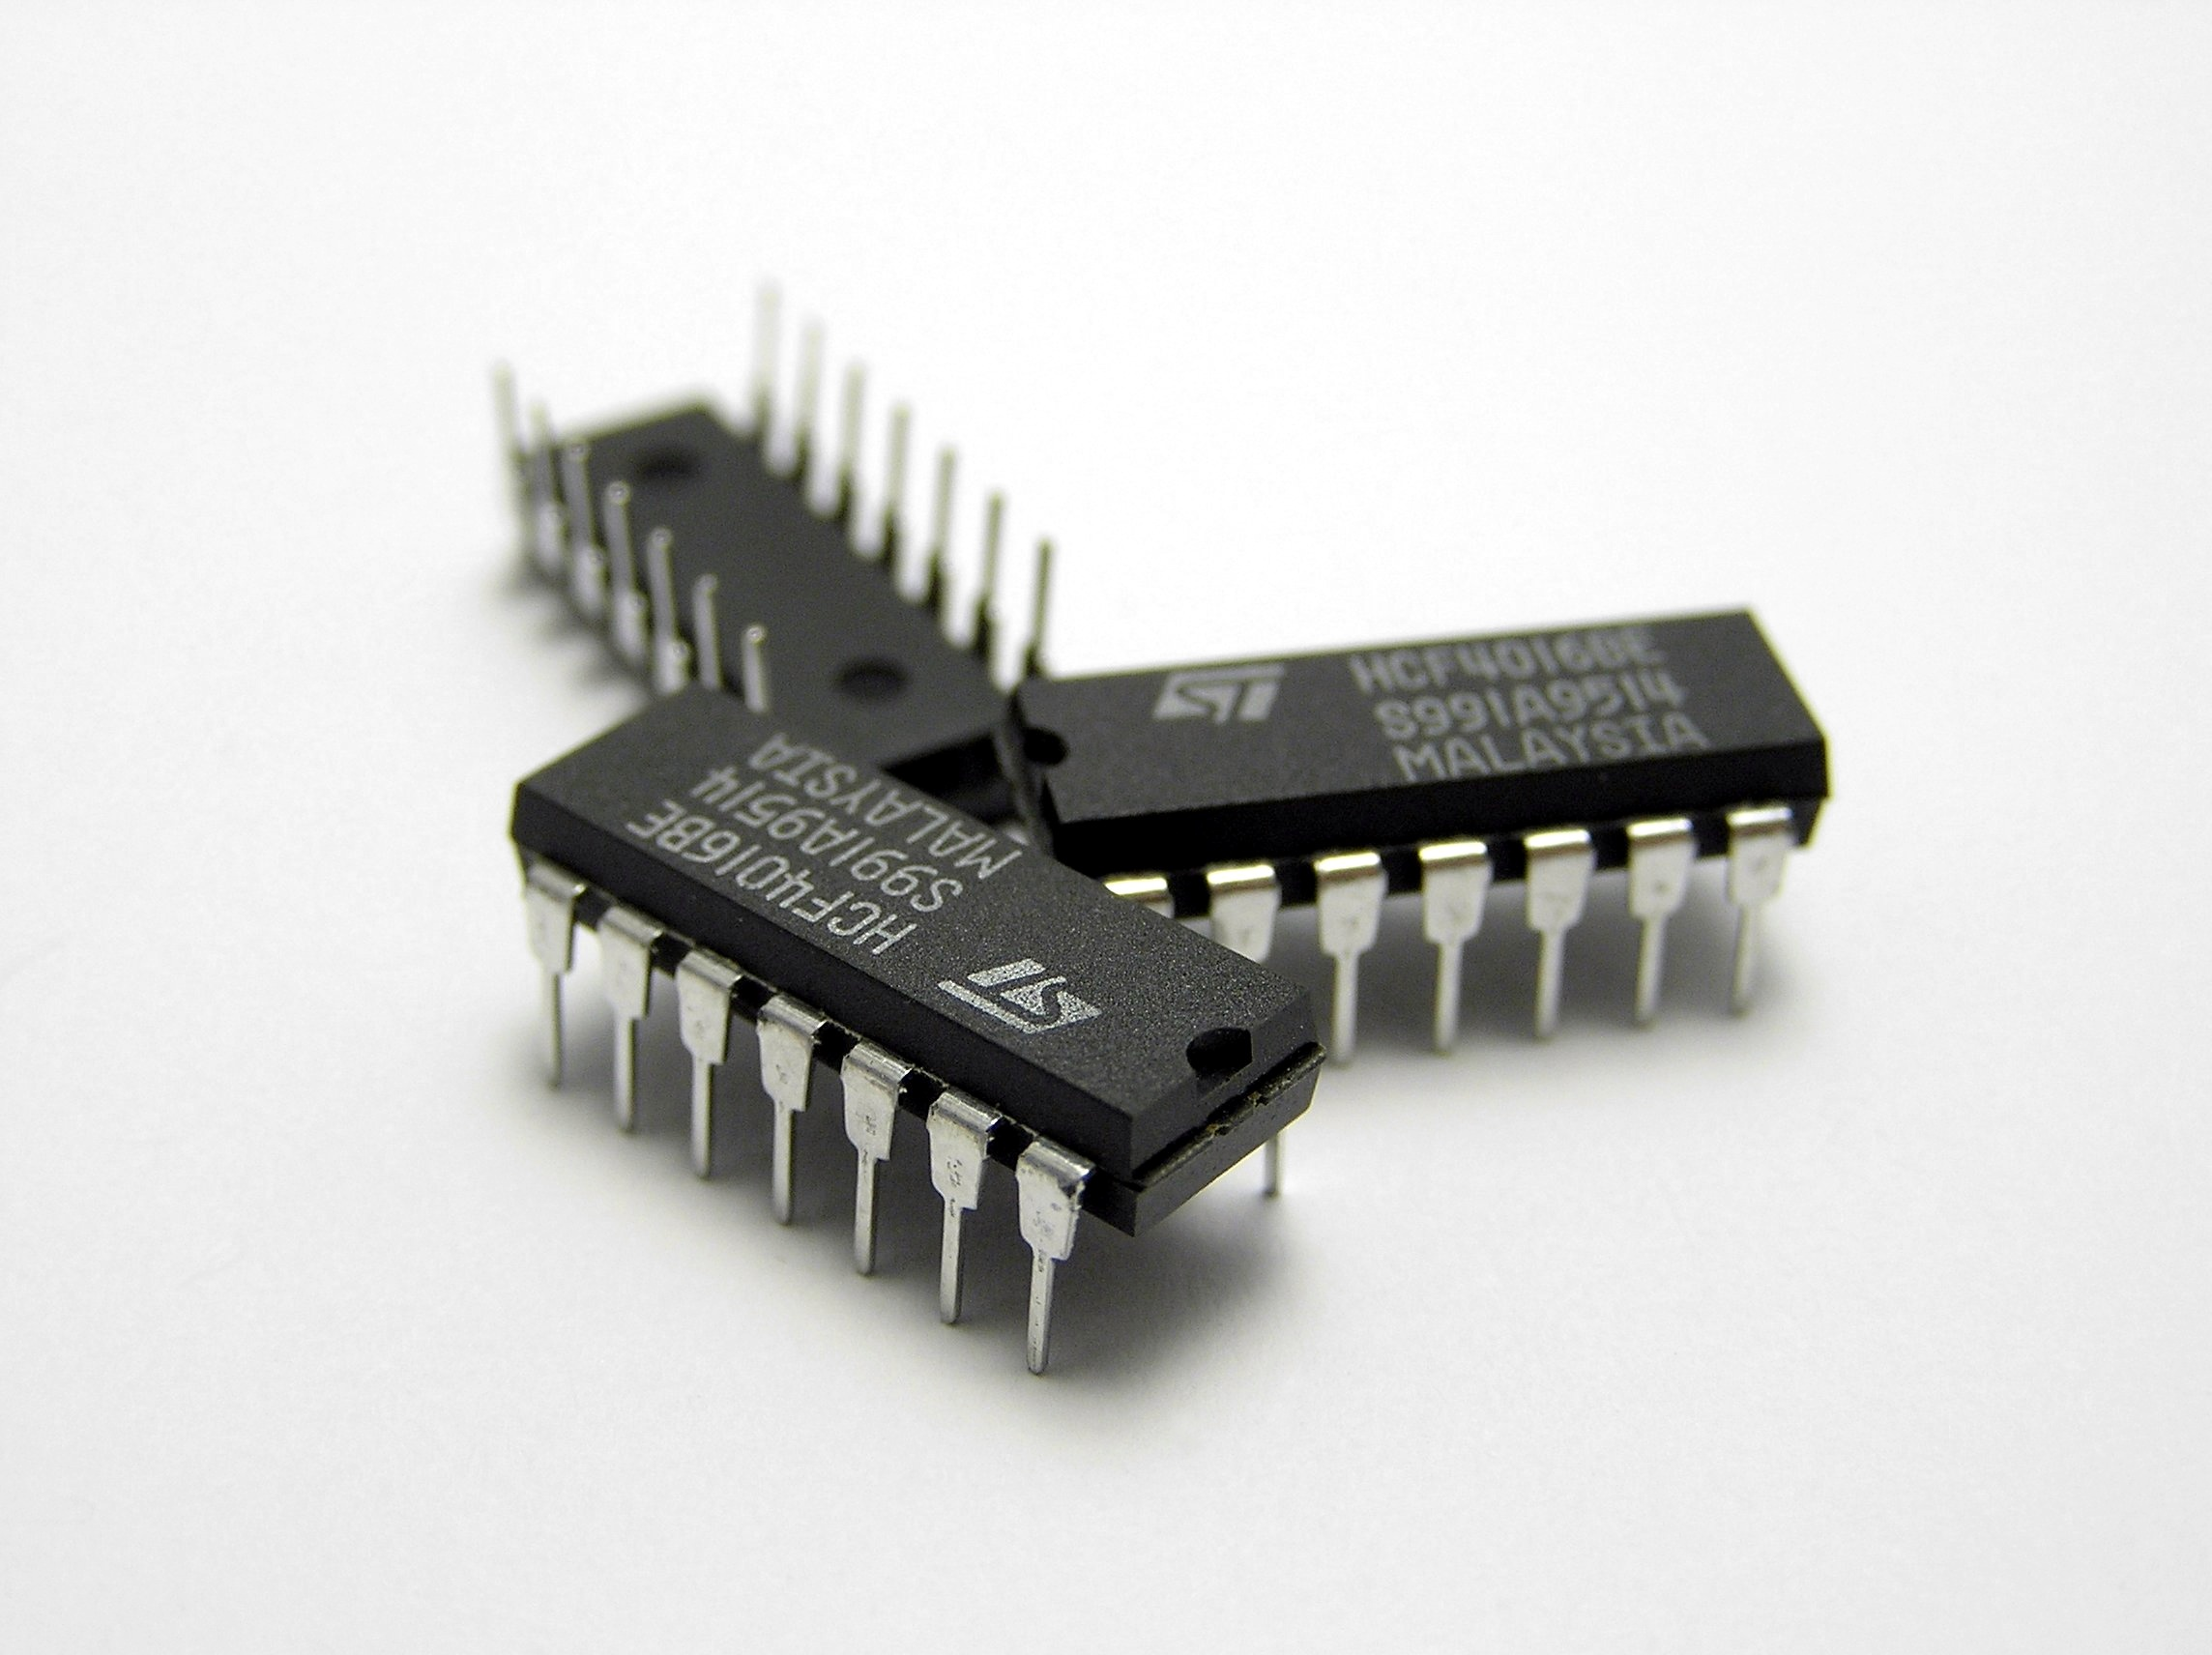
\includegraphics[width=0.5\columnwidth]{figs/Three_IC_circuit_chips.JPG}
  \caption{Three DIP integrated circuits (chips).}
%\end{floatingfigure}
\end{figure}

\subsection{Software}

\begin{itemize}
\item Forth in ROM is used as programming language.
\item Operating System is Forth.
\end{itemize}

\begin{figure*}[t!]
  \centering
  \inputfigure{figure-project-scope}
  %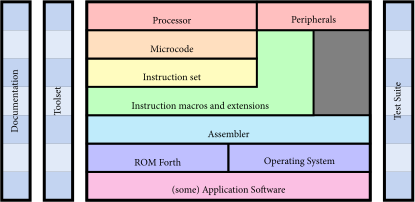
\includegraphics{figure-project-scope.png}
  \caption{\label{fig-projectscope}CFT Project scope and outline.}
\end{figure*}

% End of file.



%%%%%%%%%%%%%%%%%%%%%%%%%%%%%%%%%%%%%%%%%%%%%%%%%%%%%%%%%%%%%%%%%%%%%%%%%%%%%%%
%%%%%%%%%%%%%%%%%%%%%%%%%%%%%%%%%%%%%%%%%%%%%%%%%%%%%%%%%%%%%%%%%%%%%%%%%%%%%%%

\setcounter{chapter}{0}

\renewcommand{\thepart}{\Alph{part}}
\renewcommand{\thechapter}{\Alph{part}\arabic{chapter}}
\renewcommand{\thepage}{\Alph{part}\arabic{chapter}-\arabic{page}}
\renewcommand{\thefigure}{\Alph{part}\arabic{chapter}.\arabic{figure}}
%% \renewcommand{\theschematic}{\Alph{part}\arabic{chapter}.\arabic{schematic}}
\renewcommand{\thetable}{\Alph{part}\arabic{chapter}.\arabic{schematic}}
\renewcommand{\thepage}{\thepart\thechapter-\arabic{page}}

\ifdefined\renderpartprocessor
  \part{Processor}
  \glsresetall

  \chapter{Theoretical Description}

This chapter describes the CFT processor from a theoretical
perspective.

For a hardware description of the units described here and more minor ones
beyond the scope of a theoretical discussion, please refer
to~\ccf{chap:processor-hardware-description}. For a description of the
processor's programming model, please refer to~\ccf{chap:programming-model}.


\section{Datapath}

\begin{figure}
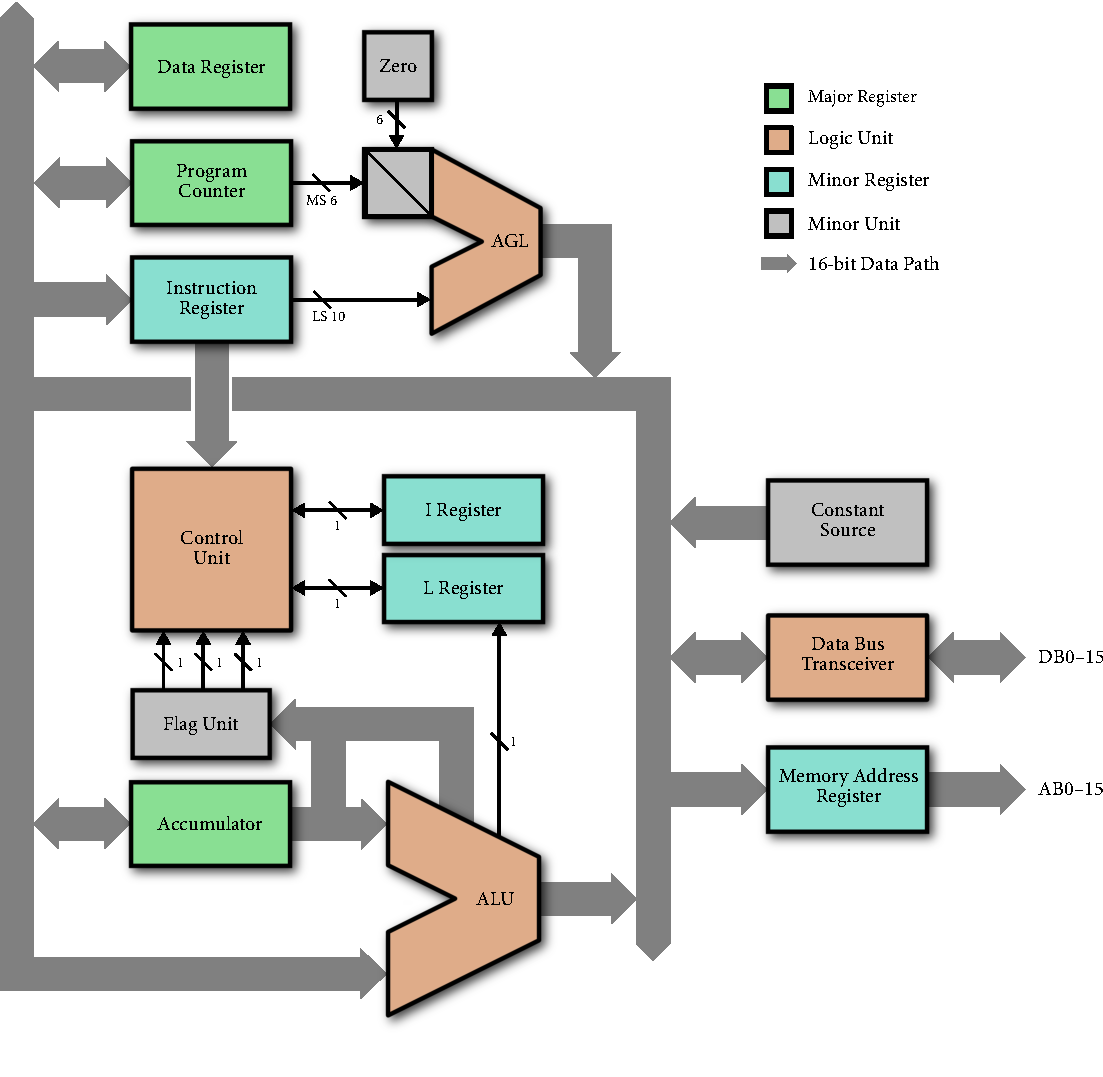
\includegraphics[width=0.95\columnwidth]{figs/datapath2.pdf}\vspace{2em}\\
\caption[CFT Datapath]{\label{fig:datapath} The CFT Datapath. }
\end{figure}

The CFT datapath, illustrated in~\fcf{fig:datapath}, is organised around a
single internal bus, the \IBUS{}. This precludes pipelining techniques, but keeps
the processor easy to reason about and implement. A number of units may either
write to the \IBUS{}, or read from it. The \IBUS{} may also be connected to the
external \DBUS{} via the Data Bus Transceiver, so that data can be exchanged
between the processor and its peripherals.

The Control Unit (centre left) is disjoint from the \IBUS{}, but controls what
other units are connected to it. To do so, it consults the values of registers
and flags.

The \ALU{} is responsible for all high-level operations performed by
the processor. It can perform a number of binary and unary
operations. All operations involve the \gls{Accumulator} (see below). Binary
operations involve the current value of the \gls{Accumulator} and the value
of the \IBUS{}. The \ALU's operations update some of the flags used by
the control Unit.

Ancillary to the \ALU{} is the Constant Store, which can provide a small
number of constant values to the \IBUS{}. These are useful for a number of
operations, such as clearing registers by assigning them the zero constant.

The Flag Unit is illustrated in the datapath as a clearing house for the values
of various flags in the processor. It does not have a corresponding physical
unit, as flags feed directly into various parts of the Control Unit, but it
helps illustrate simply how this is done.

There are three {\em major\/} registers in the datapath: the \gls{Accumulator} (\A),
the Data Register (\DR), and the Program Counter (\PC). Major registers are
16-bits wide. They may be read from or written to, incremented by one, or
decremented by one.

Of these, the \A{} is used as a general-purpose register, permanently and
directly supplying the left operand of the \ALU, and generating flags
used by the Control Unit in decision making.

The \PC{} is used to store the location in memory of the next instruction to be
executed.

The \DR{} is used to store temporarily intermediate addresses used for indirect
memory accesses.

A number of {\em minor registers} are also available. These are either narrower
than 16 bits, or have various restrictions placed on them. The Interrupt
(\Ireg{}) register is a single-bit register that controls whether asynchronous
interrupts may temporarily stop the processor. The {\em Link Register} (\Lreg)
is a versatile single-bit register: it is used as a flag, a carry out bit,
carry in bit, a borrow bit, or a shift register, and is usually treated as a
one-bit extension of the \A{} register. Finally, the \IR{} is a 16-bit
write-only\footnote{It is write-only from the point of view of the \IBUS{} only
  — the Control Unit reads its value continuously.} register permanently
connected to the Control Unit, and controlling its behaviour.

The memory Address Register (\AR{}) is a write-only 16-bit register that stores
an address, and when required, writes this address onto the \ABUS{} to
facilitate external read/write cycles.

Memory addresses used for data are calculating by the \AGL{}, which is
responsible for implementing addressing modes. The \AGL{} can generate 16-bit
addresses either close to the current instruction (by using the top bits of the
\PC{}), or near the beginning of memory (by zeroing the top bits).

\section{Major States}
\label{sec:major-states}

The major states of the processor are fairly conventional, as are the transitions between them:

\begin{description}
\item {\bfseries Reset}. The initial state of the processor. This state is
  entered asynchronously when computer is reset, and remains in this state for
  a set number of clock periods, according to the operation of the reset
  sequencer. During the reset state, slow units stabilise (after being powered
  on, or after a brown out), and numerous registers in the computer are cleared
  to sane values.
  %the \ns{RESET} line is asserted. The processor remains in this state until
  %the reset state machine deasserts \ns{RSTHOLD}, usually after a hardwired
  %number of clock cycles. In the Reset state, internal state is cleared, and
  %the \PC{} is set to the reset vector (\hex{FFF0}).

\item {\bfseries Fetch}. In this state, the processor performs a memory read to
  get the contents of the \IR, which implicitly jumps to the appropriate
  microprogram, and to the Execute state. The Fetch state is entered at the end
  of the Reset state; at the end of the Stop state once the computer is no
  longer halted; at the end of the Interrupt state once the interrupt
  microprogram has executed; and at the end of the Execute state, when the
  microprogram signals its end — the Fetch-Execute loop forms the implicit Run
  state. In fact, Fetch and Execute are not explicitly signalled: Fetch is
  simply the first memory read cycle of a microprogram, and Execute is the
  remainder. The distinction is only useful in theory\footnote{And on the front
    panel, which actually includes Fetch and Execute lights, decoded based on
    the value of the Control Unit \register{μPC}.}.

\item {\bfseries Execute}. In this state, the instruction retrieved in the
  Fetch state is executed. This state is only entered at the end of the Fetch
  state and is where all the processing is carried out. At the end of the
  Execute state, the processor usually re-enters the Fetch state to retrieve
  the next instruction, but may also enter the Interrupt state.

\item {\bfseries Interrupt}. The Interrupt state is entered at the end of the
  Execute state if an interrupt has been previously been signalled and
  interrupts are unmasked. In this state, the processor saves certain registers
  and jumps to a hardwired location holding an interrupt service routine.
  %sets the \PC{} to the hardwired interrupt vector (\hex{FFF8}).

\item {\bfseries Stop}. In this state, the processor's microprogram counter
  (\register{μPC}) is inhibited, freezing the processor. The clocks are still
  running, allowing peripherals that use them to operate. This state is entered
  while the computer is halted. The processor's design is fully static, so it
  may stay in the Stopped state indefinitely.

\end{description}

\section{The Wait State}

The Wait State is a transient, astable state. It may be entered at any time,
though it has special meaning during memory or I/O cycles and is easier to
generate during them. As long as a wait state is signalled, the control unit
protracts its current operation. Wait states are meant to be used with devices
too slow to handle the processor's read or write cycles. They allow most of the
processor to operate at its top speed, slowing down only when communicating
with such devices.


%% The Wait State is a transient state. It may be entered at any time
%% when \ns{WS} is asserted, though it has special meaning during memory
%% or I/O cycles.

%% Once the \ns{WS} signal is deasserted, the processor resumes its
%% previous operation at the next clock tick.

%% \todo{Describe this in detail.}

\begin{figure}
  \centering
  \inputfigure{figure-major-states}
  \caption[CFT Processor Major States]{\label{hard:proc:major-states}CFT Processor Major States:
    Reset (R), Fetch (F), Execute (E), Stop (S), and Interrupt (I).}
\end{figure}


\section{Processor Cycle}

Each processor cycle consists of four stages, T1-T4, each at a 90°
phase difference from the previous one, and each lasting 25\% of the
nominal clock period. With the clock running at 4~MHz, each phase
lasts $250\,\mbox{ns}/4 = 62.5\,\mbox{ns}$.

\begin{description}
\item{\bfseries T1:} the microprogram counter increments, generating a
  new microprogram address. A microcode memory lookup begins.
\item{\bfseries T2:} the microcode memory lookup concludes. With 70\,ns
  ROMs, the second phase must be used to wait for the signals to
  stabilise. As this happens, the decoding unit (which is
  asynchronous) decodes the micro-instruction vector into read enable
  signals and write strobe enable signals for the various units.
\item{\bfseries T3:} one of various things can happen at this point.
  \begin{itemize}
    \item If no data transfer is required by the micro-instruction, the
      processor goes idle.
    \item If a data transfer between internal processor units is
      needed, the unit to be read from drives the \IBUS{} with its data.
    \item If a memory or I/O read is requested, \ns{MEM} or \ns{IO} is
      asserted as appropriate. \ns{R} is also asserted at this
      time. This instructs the memory or peripheral to select chips
      and initiate a read cycle. During this phase, the memory or
      peripheral may signal a \ns{WS} to temporarily delay the onset
      of the next phase.
    \item If a memory or I/O write is requested, \ns{MEM} or \ns{IO}
      is asserted as appropriate. This instructs the memory or
      peripheral to select chips and initiate a write cycle. Data is
      driven onto the \IBUS{}, and the \DBUS{} is connected to the
      \IBUS{} to provide valid data for the external device. During
      this phase, the device may assert \ns{WS} to temporarily delay
      the onset of the next phase.
  \end{itemize}
\item{\bfseries T4:} one of various things can happen at this point.
  \begin{itemize}
  \item If no data transfer is required by the micro-instruction, the
    processor remains idle.
  \item If a data transfer between internal processor units is
    needed, the appropriate write enable signal is asserted at this
    point, and the unit latches data from the \IBUS. This also
    happens for memory or I/O reads.
  \item If a memory or I/O write is requested, \ns{W} is
      asserted. The external device latches or clocks data
      accordingly.
  \end{itemize}
\end{description}

\begin{figure*}
\centering
\inputfigure{figure-processor-cycle}
\caption[Phases of a processor cycle]{\label{fig:processor-cycle} The four phases of a processor cycle. Please note that the fetch and decode stages happen asynchronously, since microcode ROM access times are higher than 25\% of the clock period. The \DBUS{} is never accessed during the first half of the processor cycle, which allows other devices (such as a VDU or DRAM refresh circuitry) to access the bus.}
\end{figure*}

%% \section{Interrupts}

%% \chapter{Hardware Description}
%% \label{chap:processor-hardware-description}


%% The CFT processor is made up of a number of relatively simple units connected
%% in way that causes complex (and in fact, Turing Complete) emergent
%% behaviour. The units are as follows:

%% \begin{description}
%%   \item{\bfseries Clock Generator}. This simple unit generates appropriately
%%     phased clocks from one of three clock sources, and allows stopping the
%%     clock and single-stepping.

%%   \item{\bfseries Reset Sequencer}. Handles reset inputs and performs the reset
%%     sequence.

%%   \item{\bfseries Microcode Sequencer}. The nerve centre of the Control
%%     Unit. Based on a number of inputs and a microcode store, this unit outputs
%%     appropriate control signals to drive the other units in the approproriate
%%     sequence.

%%   \item{\bfseries Unit Decoders}. Decodes microcode sequencer vertical signals
%%     to strobes driving individual units.

%%   \item{\bfseries Skip/Branch Logic}. This unit implements flow control by
%%     signalling the Microcode Sequencer (when it requests this) when a microcode
%%     branch is required. This is also used to perform \gls{machine code}-level
%%     skips.

%%   \item{\bfseries Address Generation Logic}. This unit forms half of the
%%     \glspl{Addressing Mode} of the processor.

%%   \item{\bfseries Instruction Register}. Contains the bit pattern of the
%%     instruction currently being executed. This selects a microprogram for the
%%     Microcode Sequencer to run.

%%   \item{\bfseries Interrupt State Machine}. A state machine that handles
%%     interrupt requests and instructs (when appropriate) the Microcode Sequencer
%%     to jump to the interrupt microprogram.

%%   \item{\bfseries Data Bus Driver and Wait States}. A unit that connects the
%%     processor's internal bus to the external data bus, and also generates write
%%     waveforms. As a bonus, it also handles requested wait states.

%%   \item{\bfseries Address Register}. Is a write-only register that holds the
%%     addresses used to drive the external Address Bus and can drive it as
%%     required.

%%   \item{\bfseries Program Counter}. A major 16-bit register that holds the
%%     address in memory of the next instruction to execute. It supports reading,
%%     writing and increments.

%%   \item{\bfseries Data Register}. A major 16-bit register used to implement
%%     Indirect \glspl{Addressing Mode}. This register supports reading, writing,
%%     increments and decrements.

%%   \item{\bfseries Accumulator}. The single general purpose register of the CFT
%%     architecture. This register supports reading, writing, increments and
%%     decrements, and also calculates the zero and negative flags for the Control
%%     Unit and \gls{ALU}.

%%   \item{\bfseries Autoindex Logic}. This unit helps implement Autoindex mode by
%%     notifying the Microcode Sequencer when the appropriate addresses are used.

%%   \item{\bfseries I/O Device Address Decoder}. To simplify address decoding for
%%     peripherals, this unit decodes the upper eight bits of the I/O address
%%     space and provides appropriate chip select signals on the expansion bus.

%%   \item{\bfseries Link Register}. A complex single-bit register with complex
%%     set, clear and toggle inputs.

%%   \item{\bfseries ALU Operationg Decocder}. Receives signals from the
%%     Control Unit and drives appropriate parts of the \gls{ALU}.

%%   \item{\bfseries ALU Binary B Register}. Implements the right-hand register
%%     for \gls{ALU} binary operations.

%%   \item{\bfseries ALU Binary Y Register}. Implements the output register
%%     for \gls{ALU} binary operations.

%%   \item{\bfseries ALU Binary Table}. Implements the binary operation function
%%     table.

%%   \item{\bfseries ALU Unary Table}. Implements the unary operation function
%%     table.

%%   \item{\bfseries Flag Logic}. Implements the flag registers attached to the
%%     \gls{ALU}.

%%   \item{\bfseries 8 kWord Memory Banking Unit}. A simple banked memory
%%     management unit that allows 21 bits of physical memory to fit the CFT's
%%     16-bit address space.

%% \end{description}

%% \begin{figure*}
%% \includegraphics[width=0.95\textwidth]{figs/Processor-Board-A.png}\vspace{2em}\\
%% \caption[Layout of Processor Board A]{\label{fig:layout-board-a} Layout of Processor Board A.}
%% \end{figure*}
%% \begin{figure*}
%% \includegraphics[width=0.95\textwidth]{figs/Processor-Board-B.png}\vspace{2em}\\
%% \caption[Layout of Processor Board B]{\label{fig:layout-board-b} Layout of Processor Board B.}
%% \end{figure*}
%% \begin{figure*}
%% \includegraphics[width=0.95\textwidth]{figs/Processor-Board-C.png}\vspace{2em}\\
%% \caption[Layout of Processor Board C]{\label{fig:layout-board-c} Layout of Processor Board C.}
%% \end{figure*}

%% This chapter discusses the theory of operation of the actual hardware
%% implementation of the processor. It discusses how the theoretical CFT
%% architecture can be implemented as hardware. It is broken down by
%% processor unit, including the minor ones, and examines each in an
%% isolated fashion.

%% \section{Clock Generator}

%% The original intention is to run the processor at a clock rate of 4~MHz (a
%% clock period of 250~ns). This is output by the clock generator circuitry. There
%% are four clock phases, all at a 50\% duty cycle, each at a 90° phase
%% difference. For each rising clock edge, there is a synchronous, corresponding
%% falling clock edge 90° away, and vice versa. Some of these clock phases are
%% used directly in the processor (or computer) circuitry. Others are combined to
%% create specific timing pulses or strobes.

%% A 4:1 multiplexer selects one of three clock sources: the fast clock
%% (\ps{FASTCLK}, nominally at 16~MHz), a slower demonstration clock named
%% \ps{SLOWCLK} (around 200–250 Hz) and a creeping clock for testing and microcode
%% debugging called \ps{TESTCLK} (around 20–25 Hz). The multiplexer selects among
%% the three clocks with two input signals from the front panel, \ps{FPFAST} and
%% \ps{FPSLOW}. The following function table is implemented:

%% \begin{center}
%%   \zebra
%%   \begin{tabular}{*{4}{>{\textsf\bgroup}c<{\egroup}}l}
%%     %\noalign{\smallskip}\hline\noalign{\smallskip}
%%     %\hline
%%     \ps{FPSLOW} & \ps{FPFAST} & Mux AB & Clock \\
%%     %\noalign{\smallskip}\hline\noalign{\smallskip}
%%     \hline
%%     L & L & \bin{00} & \ps{SLOWCLK} \\
%%     H & L & \bin{10} & \ps{TESTCLK} \\
%%     X & H & \bin{X1} & \ps{FASTCLK} \\
%%     \hline
%%   \end{tabular}
%% \end{center}

%% To provide a sane clock selection when no front panel is connected, \ps{FPFAST}
%% is pulled high and \ps{FPSLOW} is pulled low. This selects the fast clock.

%% \paragraph{Fast Clock}

%% To ensure a stable clock with maximal accuracy, the fast clock was implemented
%% as a single-part, four pin, 16~MHz crystal oscillator. The only additional
%% component to this clock source is a 100~nF bypass capacitor.

%% \paragraph{Slow Clock}

%% There are fewer concerns about the accuracy of the slow clock, and duty cycle
%% is immaterial since clocks are subdivided and only the positive edge is used —
%% as such, only the overall {\em clock period\/} is important. Thus, it was
%% easier and more flexible to implement the slow clock using a 555 timer in its
%% standard astable configuration, as shown in~\fcf{fig:555-astable}.

%% \begin{figure}
%% \centering
%% 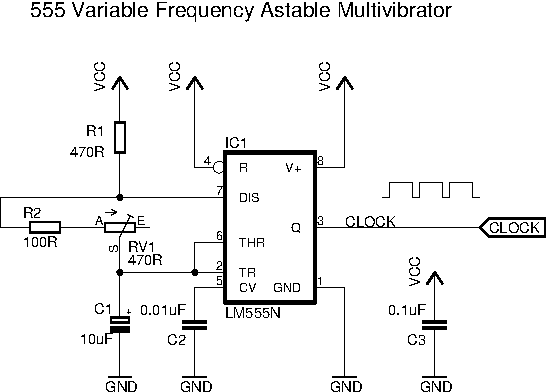
\includegraphics{figs/fig-555-astable.pdf}\\
%% \caption[LM555 in astable configuration] {\label{fig:555-astable}The popular LM555 timer in its astable
%%   configuration, with a variable frequency (and inevitable variable duty
%%   cycle). This one is configured to generate 89–215~Hz frequencies, and is used
%%   as the \ps{SLOWCLK} generator.}
%% \end{figure}

%% \paragraph{Test Clock}

%% The test clock is the same design as the slow clock — in fact, they are both
%% built around the same 556 IC (two 555 timers in one 16-pin \gls{DIP} package).


%%  Each clock source is
%% divided by four internally to generate the four clock phases.

%% \bug{\ps{FPUSTEP} needs to strobe at 2×CLK, this is not very useful.}{} \bug{The slow
%%   clock generators run at ¼ frequency.}{The best way to fix this is to change the 555
%%   capacitor to 2.2µF from 10µF, and adjust the variable resistors.}

%% \todo{Use XOR-based edge detection to generate two pulses (four edges) from one activation
%%   of the \sw{µSTEP} switch.}

%% \todo{Complete this}


%% \begin{figure}
%% \centering
%% \begin{tikztimingtable}
%%   \ns{RAWCLK} & H CL N(A1) 4{CH CL} N(A2) 4{CH CL} N(A3) 4{CH CL} N(A4) 2{CH CL} CH \\
%%   %% \CLOCK{1} (270°)  & L 8H 3{8L 8H} 4L \\
%%   %% \CLOCK{2} (180°)  & 5H 3{8L 8H} 8L \\
%%   %% \CLOCK{3} (90°)   & H 8L 3{8H 8L} 4H \\
%%   %% \CLOCK{4} (0°)    & 5L 3{8H 8L} 8H \\
%%   %% \CLOCK{5}         & L 12H 3{4L 12H} L \\
%%   %% \GUARDPULSE       & 3L ee 3{3H ee 11L ee} 3H ee 8L \\
%%   \CLOCK{1} (0°)       & 3H 3{4L 12H} 4L 6H\\
%%   \CLOCK{2} (90°)      & 7H 3{4L 12H} 4L 2H\\
%%   \CLOCK{3} (180°)     & 11H 3{4L 12H} 2L \\
%%   \CLOCK{4} (270°)     & 3L N(B1) 12H 4L N(B2) 12H 4L N(B3) 12H 4L N(B4) 10H\\
%% %
%%   \extracode
%%   \tablerules
%%   \begin{pgfonlayer}{background}
%%     \foreach \n in {1,...,4}
%%     \draw [help lines] (A\n) -- (B\n);
%%   \end{pgfonlayer}
%% \end{tikztimingtable}
%% \caption{\label{fig:clock-timing} Timing diagram of the four-phase clock generator.}
%% \end{figure}


%% \begin{figure}
%% \centering
%% \begin{tikztimingtable}
%%   \CLOCK{3}    & H CL 4{CH CL} N(A2) 4{CH CL} N(A3) 4{CH CL} N(A4) 2{CH CL} CH \\
%%   \ns{RESET}   & 10H N(A1) 3L ;[dotted] 15L; 7L H ;[dotted] 15H; 10H \\
%%   \ns{RSTHOLD} & 10H 3L ;[dotted] 15L; 8L N(B3) ;[dotted] 15L; 10H \\
%%    \IBUSn{0–15} & 10U{} N(B1) 41D{\hex{FFF0}} N(B4) 10U{} \\
%% %
%%   \extracode
%%   \tablerules
%%   \begin{pgfonlayer}{background}
%%     \foreach \n in {1,4}
%%     \draw [help lines] (A\n) -- (B\n);
%%   \end{pgfonlayer}
%% \end{tikztimingtable}
%% \caption[Reset waveform]{\label{fig:reset-timing} Reset waveform. The width of \ns{RSTHOLD} has
%%   a guaranteed, configurable minimum width and its rising edge is synchronous
%%   to the rising edge of \CLOCK{3}.}
%% \end{figure}


%% \section{Reset Logic}

%% The Reset Logic is a simple 8-bit counter, clocked from the processor clock to
%% ensure the reset pulse is synchronised with the processor sequencer.

%% A number of open drain reset inputs are combined together and fed into the
%% counter's active low reset pin. These include:

%% \begin{itemize}
%% \item The front panel \ns{FPRESET} input. This is connected to a toggle switch
%%   and allows the user to reset the computer manually.
%% \item The power supply \ps{POWEROK} signal. The power supply asserts this when
%%   the power output is healthy. The signal is clear when the power supply is
%%   still stabilising after initial power up, or when a brown-out is
%%   detected. Interpreting it as the imaginary active-low ‘\ns{POWERBAD}’ signal
%%   allows us to reset the machine on brown-outs {\em and\/} to allow for a
%%   power-on reset sequence.
%% \item When the optional reset button on the reset logic board is pressed.
%% \item When the open drain \ns{RESET} signal is asserted. This allows any number
%%   of external drivers of this signal.
%% \end{itemize}

%% When the reset signal goes low, the counter resets and starts counting. A bank
%% of jumpers connects one of the counter's binary outputs to the \ns{RSTHOLD}
%% signal. With the count reset, \ns{RSTHOLD} goes low. When the count progresses
%% enough for the selected bit to go high, \ns{RSTHOLD} goes high
%% (deasserted). This also disables the counter. At this point, the \ns{RSTHOLD}
%% pulse is complete.

%% By selecting which count bit drives \ns{RSTHOLD}, the pulse width can be controlled. In
%% theory, pulse widths of $2^n$ clock periods ($1\leq n\leq 8$) can be used. In practice,
%% because the counter is registered, and the register and count inputs are wired together,
%% the \ns{RSTHOLD} pulse lasts for one extra clock period. Also, since the reset pulse
%% arrives asynchronously, the \ns{RSTHOLD} may be up to one clock period longer yet.

%% With a clock of 4~MHz, the longest reset pulse is 64.25~ms which is fine for most uses:
%% the processor itself is very quick to reset, needing less than one clock period. Other
%% hardware, however, is not as fast. Since a reset sequence also happens when the computer
%% powers up or a brown-out is detected, an extended \ns{RSTHOLD} pulse makes the processor
%% wait for power rail and clock stabilisation (among other potential pitfalls).

%% While \ns{RSTHOLD} is active, the value \hex{FFF0} is driven onto the \IBUS{}
%% using a pair of 74x541 buffers. This is the Reset Vector. The processor uses
%% this value to reset the \PC{} to its initial value.

%% \section{Microprogram Counter}
%% \label{sec:upc}

%% The Microprogram Counter (µPC) is a simple 4-bit counter with reset and dual
%% count enables. A \HC{161} counter was selected for this. The '161 counts on the
%% positive edge of \CLOCK{1}, while the count enables are high. These are driven
%% by \ns{WS} and \ns{HALT}, both pulled up in case the two input signals are
%% physically unconnected.

%% The counter resets to zero when \ns{RSTHOLD} is asserted.

%% The \ns{END} signal and its open drain, external counterpart \ns{ENDEXT} are ANDed
%% together and fed to the '161's active low load signal (\ns{LD}). This loads the counter
%% from the \ps{P1}–\ps{P4} inputs, which are always driven low. This is effectively used to
%% reset the counter when the currently executing microprogram is finished.

%% The counter's output provides the four least significant bits of the microcode address
%% vector, the others being provided by other processor states.

%% The counter implements the following function table:

%% \begin{center}
%%   \zebra
%%   \begin{tabular}{*{6}{>{\textsf\bgroup}c<{\egroup}}l}
%%     %\noalign{\smallskip}\hline\noalign{\smallskip}
%%     %\\\hline
%%     \ps{CLOCK4} & \ns{RSTHOLD} & \ns{END} & \ns{ENDEXT} & \ns{WS} & \ns{HALT} & Function \\
%%     %\noalign{\smallskip}\hline\noalign{\smallskip}
%%     \hline
%%     X   & L & X & X & X & X & Reset counter to 0 asynchronously.\\
%%     \tU & H & L & X & X & X & Reset counter to 0.\\
%%     \tU & H & X & L & X & X & Reset counter to 0.\\
%%     \tU & H & X & X & L & X & Inhibit counting.\\
%%     \tU & H & X & X & X & L & Inhibit counting.\\
%%     \tU & H & H & H & H & H & Increment count (mod 16).\\
%%     \hline
%%   \end{tabular}
%% \end{center}



%% %\tikzset{timing/new counter={char=Q,base=16,reset char=R}}
%% \begin{figure*}
%%   \centering
%% \begin{tikztimingtable}
%%   \CLOCK{4}    & L 2{2H 2L} N(A2) 2H 2L N(A3) 2H 2L N(A4) 2H 2L N(A5) %
%%                  2H 2L N(A6) 2H 2L N(A7) 2H 2L N(A8) %
%%                  2H 2L N(A9) 5{2H 2L} N(A10) 2H 2L N(A11) %
%%                  2H 1 \\
%%   \ns{RSTHOLD} & 2H N(A1) 4L 57H \\
%%   \ns{END}     & 15H 3L 45H \\
%%   \ns{ENDEXT}  & 23Z 3L 37Z \\
%%   \ns{WS}      & 38Z 8L 17Z \\
%%   \ns{HALT}    & 47Z 8L 8Z \\
%%   \UPC         & 2U{} N(B1) 7D{\hex{0}} %
%%                  N(B2) 4D{\hex{1}} %
%%                  N(B3) 4D{\hex{2}} %
%%                  N(B4) 4D{\hex{0}} %
%%                  N(B5) 4D{\hex{1}} %
%%                  N(B6) 4D{\hex{0}} %
%%                  N(B7) 4D{\hex{1}} %
%%                  N(B8) 4D{\hex{3}} %
%%                  N(B9) 20D{\hex{3}} %
%%                  N(B10) 4D{\hex{4}} % 
%%                  N(B11) 2D{\hex{5}} \\
%%   %% \ns{WS} & 20H 3L 54H \\
%%   %% \ns{HALT} & 70H 7L \\
%% \extracode
%%  \tablerules
%%  \begin{pgfonlayer}{background}
%%    \foreach \n in {1,...,11}
%%      \draw [help lines] (A\n) -- (B\n);
%%  \end{pgfonlayer}
%% \end{tikztimingtable}
%% \caption[Microprogram Counter Waveforms]{\label{fig:upc-timing} Timing
%%   diagram of the operation of the microprogram counter (\UPC). The
%%   counter resets synchronously while \ns{RSTHOLD} is asserted. The
%%   rising edge of \CLOCK{4} clears it if either \ns{END} or \ns{ENDEXT}
%%   are asserted, and counting is inhibited when \ns{WS} or \ns{HALT}
%%   are asserted.}
%% \end{figure*}

%% \begin{figure}[tb]
%%   \centering
%%   % -*- latex -*-
\documentclass[border=200pt,class=memoir,preview]{standalone}
% -*- latex -*-

%%%%%%%%%%%%%%%%%%%%%%%%%%%%%%%%%%%%%%%%%%%%%%%%%%%%%%%%%%%%%%%%%%%%%%%%%%%%%%%
%%
%% PACKAGES
%%
%%%%%%%%%%%%%%%%%%%%%%%%%%%%%%%%%%%%%%%%%%%%%%%%%%%%%%%%%%%%%%%%%%%%%%%%%%%%%%%

\usepackage{ifxetex}
\usepackage{graphicx}

\usepackage{verbatim}
\usepackage{ifthen}
\usepackage{float}
\usepackage{floatflt}
\usepackage{lipsum}
\usepackage{layout}
\usepackage{calc}
\usepackage{rotating}
\usepackage{array}
\usepackage{color}
\usepackage[table]{xcolor}
\usepackage[includefoot]{geometry}

% Conditional packages
\ifxetex
  % Load fontspec and set fonts
  \usepackage{fontspec}
  \setmainfont{Minion Pro}
  \setsansfont{Myriad Pro}
  \setmonofont[]{Inconsolata}

  \usepackage{pdftricks}
  \usepackage{pdfpages}

  \def\HCode#1{}

\else
  \newcounter{Hfootnote}
  \newcommand\fontspec[1]{}
  %\usepackage[main=english,greek]{babel}
  \usepackage[utf8]{inputenc}
  \usepackage{newunicodechar}
  \newunicodechar{®}{\HCode{&reg;}}
  \newunicodechar{µ}{\HCode{&mu;}} % ‘micro’ (from latin-1 plane)
  \newunicodechar{μ}{\HCode{&mu;}} % mu (from Greek plane)
  \newunicodechar{–}{--}
  \newunicodechar{—}{---}
  \newunicodechar{×}{\ensuremath{\times}}
  \newunicodechar{°}{\HCode{&deg;}}
  \newunicodechar{±}{\HCode{&plusm;}}
  \newunicodechar{Ω}{\ensuremath{\Omega}}
  \newunicodechar{÷}{\ensuremath{\div}}
  %\newunicodechar{²}{\HCode{&sup2;}}
  \newunicodechar{²}{*2*}
  \newunicodechar{¼}{\HCode{&\#188;}}
  \newunicodechar{½}{\HCode{&\#189;}}
  \newunicodechar{≤}{\HCode{ &le; }}
  \newunicodechar{≥}{\HCode{ &ge; }}
  \newunicodechar{≠}{\HCode{ &ne; }}
\fi

%%%%%%%%%%%%%%%%%%%%%%%%%%%%%%%%%%%%%%%%%%%%%%%%%%%%%%%%%%%%%%%%%%%%%%%%%%%%%%%
%%
%% TABLES
%%
%%%%%%%%%%%%%%%%%%%%%%%%%%%%%%%%%%%%%%%%%%%%%%%%%%%%%%%%%%%%%%%%%%%%%%%%%%%%%%%

\renewcommand*\arraystretch{1.25}
\newcolumntype{P}[1]{>{\raggedright\arraybackslash}p{#1}}


%%%%%%%%%%%%%%%%%%%%%%%%%%%%%%%%%%%%%%%%%%%%%%%%%%%%%%%%%%%%%%%%%%%%%%%%%%%%%%%
%%
%% FIGURE DRAWING WITH PGF/TIKZ
%%
%%%%%%%%%%%%%%%%%%%%%%%%%%%%%%%%%%%%%%%%%%%%%%%%%%%%%%%%%%%%%%%%%%%%%%%%%%%%%%%

\ifxetex
  \usepackage{pgf}
  \usepackage{tikz}
  \usepackage{rotating}
  \usepackage[absolute]{textpos}

  %\usetikzlibrary{arrows,positioning,automata,shadows,fit,shapes,counters}
  \usetikzlibrary{arrows,positioning,automata,shadows,fit,shapes,patterns}
  \usetikzlibrary{shadows.blur}
  %\usetikzlibrary{external}
  %\tikzexternalize[prefix=tikz/]
  %\tikzset{external/system call={xelatex \tikzexternalcheckshellescape -halt-on-error -interaction=batchmode -jobname "\image" "\texsource"}}
  \usepackage{standalone}

  \usepackage{tikz-timing}[2009/07/28]
  \usetikztiminglibrary{either}[2009/07/28]
  \tikzset{>=latex}
  \tikzset{timing/z/.append style={black},}
  \tikzset{timing/.append style={x=1ex, y=2ex, line cap=round, line join=round, line width=1.3pt}}
  \tikzset{timing/slope=0.33}
  \tikzstyle{semithick}=[line width=1pt]
  \tikzstyle{heavy}=[line width=2pt]
  \tikzstyle{heavy outline}=[line width=3.5pt]
  \tikzstyle{plot line}=[line width=4pt]
  \tikzstyle{arrow}=[semithick]
  \tikzstyle{thick arrow}=[heavy]
  \tikzstyle{thick outline arrow}=[thick arrow, heavy outline, color=white, draw opacity=0.8]
  \tikzstyle{help lines}=[dotted, line width=0.5pt]
  \tikzstyle{col1}=[draw=p1,fill=p1!60]
  \tikzstyle{col2}=[draw=p2,fill=p2!60]
  \tikzstyle{col3}=[draw=p3,fill=p3!60]
  \tikzstyle{col4}=[draw=p4,fill=p4!60]
  \tikzstyle{col5}=[draw=p5,fill=p5!60]
  \tikzstyle{col6}=[draw=p6,fill=p6!60]
  \tikzstyle{dropshadow}=[] % shade,blur shadow={shadow blur steps=5, shadow blur extra rounding=1.3pt}]
  \tikzset{fsmstate/.style={state,rectangle,rounded corners,dropshadow,minimum width=10em,line width=1pt}}
  % Create a hatch pattern
  \newlength{\hatchspread}
  \newlength{\hatchthickness}
  % declaring the keys in tikz
  \tikzset{hatchspread/.code={\setlength{\hatchspread}{#1}},
           hatchthickness/.code={\setlength{\hatchthickness}{#1}}}
  \tikzset{hatchspread=3pt,
           hatchthickness=0.4pt}
  \pgfdeclarepatternformonly[\hatchspread,\hatchthickness]% variables
     {hatch}% name
     {\pgfqpoint{-2\hatchthickness}{-2\hatchthickness}}% lower left corner
     {\pgfqpoint{\dimexpr\hatchspread+2\hatchthickness}{\dimexpr\hatchspread+2\hatchthickness}}% upper right corner
     {\pgfqpoint{\hatchspread}{\hatchspread}}% tile size
     {% shape description
      \pgfsetlinewidth{\hatchthickness}
      \pgfpathmoveto{\pgfqpoint{0pt}{\hatchspread}}
      \pgfpathlineto{\pgfqpoint{\dimexpr\hatchspread+0.15pt}{-0.15pt}}
      \pgfusepath{stroke}
     }
\fi


%%%%%%%%%%%%%%%%%%%%%%%%%%%%%%%%%%%%%%%%%%%%%%%%%%%%%%%%%%%%%%%%%%%%%%%%%%%%%%%
%%
%% HYPERREF
%%
%%%%%%%%%%%%%%%%%%%%%%%%%%%%%%%%%%%%%%%%%%%%%%%%%%%%%%%%%%%%%%%%%%%%%%%%%%%%%%%

\makeatletter
\@ifpackageloaded{standalone}{}{
  \ifxetex
    \usepackage[CJKbookmarks,bookmarks=true,bookmarksopen=true,pdfpagelabels,pdfstartpage=1]{hyperref}
  \else
    \usepackage[tex4ht]{hyperref}
  \fi
}

\let\old@part\part
\renewcommand\part[1]{%
  \setcounter{chapter}{0}%
  \old@part{#1}%
}
%\renewcommand*{\theHchapter}{\thepart.\thechapter}
\makeatother


%%%%%%%%%%%%%%%%%%%%%%%%%%%%%%%%%%%%%%%%%%%%%%%%%%%%%%%%%%%%%%%%%%%%%%%%%%%%%%%
%%
%% INDEX AND GLOSSARY
%%
%%%%%%%%%%%%%%%%%%%%%%%%%%%%%%%%%%%%%%%%%%%%%%%%%%%%%%%%%%%%%%%%%%%%%%%%%%%%%%%

\usepackage{makeidx}
% Glossaries
\usepackage[acronym]{glossaries}
%\makeindex
%\makeglossaries
\input{glossary}
%\newcommand\gls[1]{#1}
%\newcommand\glsresetall{}
\ifxetex
  \glsSetCompositor{-}
  \renewcommand{\delimR}{–}
\fi


%%%%%%%%%%%%%%%%%%%%%%%%%%%%%%%%%%%%%%%%%%%%%%%%%%%%%%%%%%%%%%%%%%%%%%%%%%%%%%%
%%
%% LISTINGS OF THINGS
%%
%%%%%%%%%%%%%%%%%%%%%%%%%%%%%%%%%%%%%%%%%%%%%%%%%%%%%%%%%%%%%%%%%%%%%%%%%%%%%%%

% Lists of things (memoir already includes this if running XeTeX)
\ifxetex
  \relax
\else
  \usepackage{tocloft}
\fi


% Listings
\usepackage{minted}
\newminted{deb}{fontsize=\small}
\newminted{cftasm}{fontsize=\small}
\newminted{c}{fontsize=\small}
\newminted{forth}{fontsize=\small}
\newminted{intr}{fontsize=\small}
\newminted{mcasm}{fontsize=\small}
\newmintedfile{mcasm}{linenos=true,fontsize=\small}

\ifxetex
  \relax
\else

% Modify the minted way of invoking pygmentize if running with
% HTLatex. We'll be converting listings DIRECTLY to HTML and importing
% them into the TeX4ht output with specials.
  \makeatletter
  \newcounter{minted@temp}
  \renewcommand\minted@pygmentize[2][\jobname.pyg]{
    \stepcounter{minted@temp}
    \def\minted@cmd{pygmentize -l #2 -f html -F tokenmerge
      \minted@opt{gobble} \minted@opt{texcl} \minted@opt{mathescape}
      \minted@opt{startinline} \minted@opt{funcnamehighlighting}
      \minted@opt{linenos} -P "verboptions=\minted@opt{extra}"
      -o \jobname-\arabic{minted@temp}.out.pyg #1}
    \immediate\write18{\minted@cmd}
    % Remove kludgy markup hints (four or more @)
    \immediate\write18{sed -i -e s/@@@@//g \jobname-\arabic{minted@temp}.out.pyg}
    % For debugging, uncomment:
    %\immediate\typeout{\minted@cmd}
    \ifthenelse{\equal{\minted@opt@bgcolor}{}}
     {}
     {\begin{minted@colorbg}{\minted@opt@bgcolor}}
     \HCode{<div class="minted #2">}
     \special{t4ht*<\jobname-\arabic{minted@temp}.out.pyg} % Import the HTML output
     \HCode{</div>}
    \ifthenelse{\equal{\minted@opt@bgcolor}{}}
     {}
     {\end{minted@colorbg}}
    %\DeleteFile{\jobname.out.pyg}
  }
  \makeatother
\fi


% Old-style listings
\usepackage{listings}
\lstset{%
  xleftmargin=35pt,
  xrightmargin=5pt,
  basicstyle={\ttfamily},
  backgroundcolor=\color{cfthl!25},
  rulecolor=\color{cfthl!25},
  framesep=5pt,
  rulesep=5pt,
  frame=tlrb,
  framexleftmargin=10pt,
  flexiblecolumns=true,
  keepspaces=true,
  numbers=left,
  numbersep=5pt,
  numberstyle={\scriptsize\sffamily\color{cftlight}}
}


%%%%%%%%%%%%%%%%%%%%%%%%%%%%%%%%%%%%%%%%%%%%%%%%%%%%%%%%%%%%%%%%%%%%%%%%%%%%%%%
%%
%% COLOURS
%%
%%%%%%%%%%%%%%%%%%%%%%%%%%%%%%%%%%%%%%%%%%%%%%%%%%%%%%%%%%%%%%%%%%%%%%%%%%%%%%%

\definecolor{r0}{rgb}{0.33, 0.1, 0.1}
\definecolor{r1}{rgb}{1, 0.3, 0.3}

\definecolor{g0}{rgb}{0.1, 0.33, 0.1}
\definecolor{g1}{rgb}{0.3, 1, 0.3}

\definecolor{cftdark}{cmyk}{0,0.42,0.72,0.84}
\definecolor{cftoutline}{cmyk}{0,0.43,0.72,0.53}
\definecolor{cftlight}{cmyk}{0,0.43,0.72,0.22}
\definecolor{cfthl}{rgb}{.89,.698,.529}

\definecolor{darkblue}{RGB}{0,0,128}
\definecolor{caution}{RGB}{192,0,0}

% Graph colours

\definecolor{p1}{rgb}{0.863, .729, .318} % dcb951
\definecolor{p2}{rgb}{.792, .514, .251}  % c98340
\definecolor{p3}{rgb}{.667, .314, .176}  % aa502c
%\definecolor{p4}{rgb}{.475, .102, .098}
\definecolor{p4}{rgb}{.675, .239, .239}  % ac3d3b
\definecolor{p5}{rgb}{.435, .443, .267}  % 8e9158
\definecolor{p6}{rgb}{.345, .427, .568}  % 586d91


% End of file.

% -*- latex -*-


%%%%%%%%%%%%%%%%%%%%%%%%%%%%%%%%%%%%%%%%%%%%%%%%%%%%%%%%%%%%%%%%%%%%%%%%%%%%%%%
%%
%% WORKAROUNDS
%%
%%%%%%%%%%%%%%%%%%%%%%%%%%%%%%%%%%%%%%%%%%%%%%%%%%%%%%%%%%%%%%%%%%%%%%%%%%%%%%%

%% \ifxetex
%%   % XeTeX doesn't have HTML output, of course.
%%   \def\HCode#1{}
%% \else
%%   % This is a hack.
%%   \newcounter{Hfootnote}
%% \fi



%%%%%%%%%%%%%%%%%%%%%%%%%%%%%%%%%%%%%%%%%%%%%%%%%%%%%%%%%%%%%%%%%%%%%%%%%%%%%%%
%%
%% HTML GENERATION
%%
%%%%%%%%%%%%%%%%%%%%%%%%%%%%%%%%%%%%%%%%%%%%%%%%%%%%%%%%%%%%%%%%%%%%%%%%%%%%%%%

\ifxetex
  \def\texonly#1{#1}
  \def\htmlonly#1{}
  \newenvironment{htmldiv}[1]{}{}
  \newcommand{\htmlspan}[2]{#2}
  \newcommand{\htmlbreak}{}
\else
  \def\texonly#1{}
  \def\htmlonly#1{#1}
  \newenvironment{htmldiv}[1]{\HCode{<div class="#1">}}{\HCode{</div>}}
  \newcommand{\htmlspan}[2]{\HCode{<span class="#1">}{#2}\HCode{</span>}}
  \newcommand{\htmlbreak}{\HCode{<div class="break" />}}
\fi


%%%%%%%%%%%%%%%%%%%%%%%%%%%%%%%%%%%%%%%%%%%%%%%%%%%%%%%%%%%%%%%%%%%%%%%%%%%%%%%
%%
%% LINKING TO LOCATIONS IN THE DOCUMENT
%%
%%%%%%%%%%%%%%%%%%%%%%%%%%%%%%%%%%%%%%%%%%%%%%%%%%%%%%%%%%%%%%%%%%%%%%%%%%%%%%%

% Use hyperlinking when rendering PDFs
\newcommand{\barecf}[1]{\hyperref[#1]{\ref*{#1}}}

\newcommand{\cf}[2][section]{\hyperref[#2]{%
  \ifxetex%
    \ifthenelse{\equal{\pageref*{#2}}{\thepage}}%
               {#1 \ref*{#2}}%
               {#1 \ref*{#2} (p.~\pageref*{#2})}%
  \else%
               {#1 \ref*{#2}}%
  \fi%
}}

\newcommand{\cfp}[2][section]{\hyperref[#2]{%
  \ifxetex%
    \ifthenelse{\equal{\pageref*{#2}}{\thepage}}%
      {#1 \ref*{#2}}%
      {#1 \ref*{#2}, p.~\pageref*{#2}}%
  \else
     {#1 \ref*{#2}}%
  \fi%
}}

\newcommand{\fcf}[1]{\cf[figure]{#1}}
\newcommand{\fcfp}[1]{\cfp[figure]{#1}}
\newcommand{\tcf}[1]{\cf[table]{#1}}
\newcommand{\tcfp}[1]{\cfp[table]{#1}}
\newcommand{\ccf}[1]{\cf[chapter]{#1}}
\newcommand{\ccfp}[1]{\cfp[chapter]{#1}}
%
\newcommand{\npcf}[2][section]{\hyperref[#2]{#1 \ref*{#2}}}
\newcommand{\appcf}[1]{\cf[appendix]{#1}}
\newcommand{\ecf}[1]{\cf[equation]{#1}}
\newcommand{\algcf}[1]{\cf[algorithm]{#1}}
\newcommand{\npappcf}[1]{\npcf[appendix]{#1}}
\newcommand{\npccf}[1]{\npcf[chapter]{#1}}
\newcommand{\npfcf}[1]{\npcf[figure]{#1}}
\newcommand{\nptcf}[1]{\npcf[table]{#1}}
\newcommand{\npecf}[1]{\npcf[equation]{#1}}
\newcommand{\npalgcf}[1]{\npcf[algorithm]{#1}}



%%%%%%%%%%%%%%%%%%%%%%%%%%%%%%%%%%%%%%%%%%%%%%%%%%%%%%%%%%%%%%%%%%%%%%%%%%%%%%%
%%
%% LISTS OF THINGS
%%
%%%%%%%%%%%%%%%%%%%%%%%%%%%%%%%%%%%%%%%%%%%%%%%%%%%%%%%%%%%%%%%%%%%%%%%%%%%%%%%

%% %%%\addtolength\cftfignumwidth{1.5em}
\ifxetex
  \makeatletter
  \renewcommand*\l@section{\@dottedtocline{1}{1.5em}{2.3em}}
  \renewcommand*\l@subsection{\@dottedtocline{2}{3.8em}{3.2em}}
  \renewcommand*\l@subsubsection{\@dottedtocline{3}{7.0em}{4.1em}}
  \renewcommand*\l@paragraph{\@dottedtocline{4}{10em}{5em}}
  \renewcommand*\l@subparagraph{\@dottedtocline{5}{12em}{6em}}
  \setcounter{maxsecnumdepth}{3}

  \renewcommand{\@pnumwidth}{3em}
  \renewcommand{\@tocrmarg}{4em}
  \makeatother
\else
  \relax
\fi

%
% Schematics
%

\newcommand\listschematicname{List of Schematics} 
\newcommand{\schematic}[1]{%
  \refstepcounter{schematic}%
  \par\noindent\textbf{Schematic \theschematic. #1}
  \addcontentsline{los}{section}{\protect\numberline{\theschematic}#1}\par%
}
\newcommand{\listofschematics}{\listofschematic}

%
% I/O Ports
%

\newcommand\listioportname{List of Input/Output Ports} 
\newlistof{listofioport}{loioport}{\listioportname}
%% \newcommand{\registerioport}[1]{%
%%   \refstepcounter{ioport}%
%%   \addcontentsline{loioport}{section}{\protect\numberline{\ }%
%% }
\newcommand\listofioports\listofioport



\newcommand\caution[1]{\textcolor{caution}{\textbf{#1}}}
%\newcommand\todo[1]{\textcolor{caution}{\bf{TODO: #1}}}

\ifxetex
  \newenvironment{obsoleted}{}{}
\else
  \newenvironment{obsoleted}{\begin{htmldiv}{obsoleted box}}{\end{htmldiv}}
\fi

%
% Tasks
%

\newcommand\listtasksname{List of Incomplete Tasks} 
\newlistof{listoftask}{lotasks}{\listtasksname}
\newcounter{task}

\ifxetex
  \newcommand{\todo}[1]{%
    \refstepcounter{task}%
    {\textcolor{caution}{\textbf{TODO: #1}}}
    \addcontentsline{lotasks}{section}{\protect\numberline{\arabic{task}}To Do: #1}\par%
  }
  \newcommand{\bug}[2]{%
    \refstepcounter{task}%
    {\textcolor{caution}{\textbf{BUG: #1 #2}}}
    \addcontentsline{lotasks}{section}{\protect\numberline{\arabic{task}}Bug: #1}\par%
  }
\else
  \newcommand{\todo}[1]{%
    \refstepcounter{task}%
    {\htmlspan{todo}{#1}}%
  }
  \newcommand{\bug}[2]{%
    \refstepcounter{task}%
    {\htmlspan{bug}{#1 #2}}%
  }
\fi
\newcommand\listoftasks\listoftask

%
% Data structures
%

\newcommand\listdatastructurename{List of Data Structures} 
\newlistof{listofdatastructure}{lods}{\listdatastructurename}
\newcounter{datastructure}
%\newcommand{\datastructure}[1]{%
%  \refstepcounter{datastructure}%
%  \par\noindent\textbf{Data Structure \thedatastructure. #1}
%  \addcontentsline{lods}{section}{\protect\numberline{\thedatastructure}#1}\par%
%}
\newcommand\listofdatastructures\listofdatastructure


%%%%%%%%%%%%%%%%%%%%%%%%%%%%%%%%%%%%%%%%%%%%%%%%%%%%%%%%%%%%%%%%%%%%%%%%%%%%%%%
%%
%% LISTINGS
%%
%%%%%%%%%%%%%%%%%%%%%%%%%%%%%%%%%%%%%%%%%%%%%%%%%%%%%%%%%%%%%%%%%%%%%%%%%%%%%%%

\newcommand\lstkbd[1]{%
  \ifxetex%
    \ensuremath{\mathbf{\textbf{#1}}}%
  \else%
    \htmlspan{input}{#1 }%
  \fi%
}
%\newcommand\lstfkbd[1]{\underline{\mathbf{\textbf{#1}}}}
\newcommand\lstfkbd[1]{\color{cftoutline}{\mathbf{\textbf{#1}}}}
\ifxetex
  \lstset{%
          keywordstyle=\fontspec{Inconsolata Bold},%
          keywordstyle=[2]\color{cftoutline}\fontspec{Inconsolata Bold},%
          keywordstyle=[3]\fontspec{Inconsolata Bold},%
          commentstyle=\color{cftlight}%
  }
\else
  \lstset{%
          keywordstyle=\textbf,%
          keywordstyle=[2]\textbf,%
          keywordstyle=[3]\textit,%
          commentstyle=\texttt%
  }
\fi
\lstdefinestyle{deb}{
  mathescape=true,
  numbers=none,
  moredelim=*[s][\textbf]{[}{]}
}
\lstdefinestyle{forthprogram}{}
\lstdefinelanguage{cftasm}{%
        mathescape=true,
        morekeywords={TRAP,IOT,LOAD,STORE,IN,OUT,JMP,JSR,ADD,AND,OR,%
                      XOR,OP1,OP2,ISZ,LIA,R,I,IFL,IFV,CLA,CLL,NOT,%
                      INC,CPL,RBL,RBR,RNL,RNR,NOP,SNA,SZA,SSL,SSV,SKIP,%
                      SNN,SNZ,SCL,SCV,CLI,SEI,SEL,NEG,ING,LI,SPA,SNP,RET,%
                      RTT,RTI,SBL,SBR},%
        morekeywords=[2]{.equ,.reg,.include,.word,.fill,%
                      .str,.data,.strp,.strn,.page,.macro,.end},%
        alsoletter=.,%
        sensitive=false,%
        morecomment=[l]{/},%
        morecomment=[l]{;},%
}

\lstdefinestyle{longmcasm}{%
        language=mcasm,
        xleftmargin=25pt,
        xrightmargin=5pt,
        framexleftmargin=20pt,
        basicstyle={\footnotesize\ttfamily},
}
\lstdefinelanguage{mcasm}{%
        mathescape=false,
        morekeywords={cond,field,signal,start,hold},%
        morekeywords=[2]{\#define,\#ifdef,\#endif,\#if,\#undef,\#line,\#warning,\#warn,\#error},%
        morekeywords=[3]{INT,RST,V,L,OP,I,SKIP,INC,uaddr},%
        alsoletter=\#,%
        sensitive=false,%
        morecomment=[l]{//},%
        %morecomment=[s]{( }{ )},%
}


\lstdefinelanguage{forth}{%
        mathescape=true,
        %morekeywords={TRAP,IOT,LOAD,STORE,IN,OUT,JMP,JSR,ADD,AND,OR,%
        %              XOR,OP1,OP2,ISZ,LIA,R,I,IFL,IFV,CLA,CLL,NOT,%
        %              INC,CPL,RBL,RBR,RNL,RNR,NOP,SNA,SZA,SSL,SSV,SKIP,%
        %              SNN,SNZ,SCL,SCV,CLI,SEI,SEL,NEG,ING,LI,SPA,SNP,RET,%
        %              RTT,RTI,SBL,SBR},%
        morekeywords=[3]{ok}
        %alsoletter=.,%
        sensitive=false,%
        %morecomment=[l]{\},%
        %morecomment=[s]{( }{ )},%
}
\newcommand\notes[1]{{\small\verbatiminput{#1}}}


%%%%%%%%%%%%%%%%%%%%%%%%%%%%%%%%%%%%%%%%%%%%%%%%%%%%%%%%%%%%%%%%%%%%%%%%%%%%%%%
%%
%% GRAPHICS
%%
%%%%%%%%%%%%%%%%%%%%%%%%%%%%%%%%%%%%%%%%%%%%%%%%%%%%%%%%%%%%%%%%%%%%%%%%%%%%%%%

% This includes a TikZ figure (if compiling with XeTeX), or a static
% PNG image (for htLaTeX).
\ifxetex
  \newcommand{\inputfigure}[2][]{\input{#2}}
\else
  %% \newcommand{\inputfigure}[2][]{%
  %%   \begin{htmldiv}{includegraphics png}%
  %%     \includegraphics{#2.png}%
  %%   \end{htmldiv}%
  %% }
  \newcommand{\inputfigure}[2][]{%
    \begin{htmldiv}{includegraphics svg}%
      %\special{t4ht*<#2.svg}
      \HCode{<img src="#2.svg" />}
    \end{htmldiv}%
  }
\fi


% This includes a PDF image (for PDF generation), or a PNG
% (autoconverted from the PDF).
\ifxetex
  \newcommand{\includeimage}[2]{\includegraphics[#1]{#2.pdf}}
\else
  \newcommand{\includeimage}[2][]{%
    \begin{htmldiv}{includegraphics png}%
      \includegraphics[#1]{#2.png}%
    \end{htmldiv}%
  }
\fi

\ifxetex
  \newcommand{\includelarge}[2]{\includegraphics[#1]{#2}}
\else
  \newcommand{\includelarge}[2][]{%
    \begin{htmldiv}{includegraphics large jpeg}%
      \includegraphics[#1]{#2}%
    \end{htmldiv}%
  }
\fi

\ifxetex
  \newcommand{\includesmall}[2]{\includegraphics[#1]{#2}}
\else
  \newcommand{\includesmall}[2][]{%
    \begin{htmldiv}{includegraphics small jpeg}%
      \includegraphics[#1]{#2}%
    \end{htmldiv}%
  }
\fi

%%%%%%%%%%%%%%%%%%%%%%%%%%%%%%%%%%%%%%%%%%%%%%%%%%%%%%%%%%%%%%%%%%%%%%%%%%%%%%%
%%
%% TYPOGRAPHY
%%
%%%%%%%%%%%%%%%%%%%%%%%%%%%%%%%%%%%%%%%%%%%%%%%%%%%%%%%%%%%%%%%%%%%%%%%%%%%%%%%

\newcommand\textcond{%
  \ifxetex%
    \fontspec{Myriad Pro Condensed}%
  \else%
    \relax%
  \fi%
}


% Hypertext
\newcommand\hyperemail[1]{\sffamily\href{mailto:#1}{#1}}
\newcommand\link[1]{\sffamily\href{http://#1}{#1}}
\newcommand\ahref[2]{\sffamily\href{#1}{#2}}

% Basic stuff
\newcommand\hex[1]{\textsf{#1}}
\newcommand\bin[1]{\textsf{#1}}

% Signals
\newcommand\tU{$\uparrow$}
\newcommand\tD{$\downarrow$}
\ifxetex
  \newcommand{\nsni}[1]{$\overline{\mbox{\textsf{{#1}}}}$}
  \newcommand{\psni}[1]{\textsf{#1}}
\else
  \newcommand{\nsni}[1]{\htmlspan{signal neg}{#1}}
  \newcommand{\psni}[1]{\htmlspan{signal}{#1}}
\fi
\newcommand{\ps}[1]{\index{#1@\psni{#1}}%
  \psni{#1}}
\newcommand{\ns}[1]{\index{#1@{$\protect\overline{\protect\mbox{\textsf{#1}}}$}}%
  \nsni{#1}}
\newcommand\BUS[2]{\ps{#1}$_{\mbox{\scriptsize #2}}$}
\newcommand\nBUS[2]{\ns{#1}$_{\mbox{\scriptsize #2}}$}

% Less than basic stuff
\newcommand{\asm}[1]{\texttt{#1}}
\newcommand{\register}[1]{\textsf{#1}\index{Registers!#1}}
\newcommand{\bus}[1]{{#1}}
\newcommand{\unit}[1]{{#1}}
\newcommand{\board}[1]{#1\index{Boards!#1}}
\newcommand{\lt}[1]{\textsf{#1}}
\newcommand{\sw}[1]{\textsf{#1\index{Switch, front panel!#1}}}
\newcommand{\instr}[1]{\asm{#1}}
\newcommand{\HC}[1]{\chip{74HC{#1}}}
\newcommand{\HCT}[1]{\chip{74HCT{#1}}}
\newcommand{\chip}[1]{#1\index{#1}}
\newcommand{\schpt}[1]{#1\textsf{#1}}
\newcommand\field[1]{\textsf{#1}}
\newcommand\port[1]{\textsf{#1}}
\newcommand\bit[1]{{\texttt{#1}}}

% CFT input and output typesetting
\newcommand\cftin[1]{\textsf{#1}}
\newcommand\cftout[1]{\textsf{#1}}
\let\cftcode\cftout
\let\cftkbd\cftin

% Machine registers
\newcommand\A{\register{AC}}
\newcommand\AC{\A}
\newcommand\DR{\register{DR}}
\newcommand\PC{\register{PC}}
\newcommand\IR{\register{IR}}
\newcommand\AR{\register{AR}}
\newcommand\MAR{\AR}
\newcommand\Areg{\A}
\newcommand\Ireg{\register{I}}
\newcommand\Lreg{\register{L}}
\newcommand\Zreg{\register{Z}}
\newcommand\Vreg{\register{V}}
\newcommand\Nreg{\register{N}}

% Buses and units
\newcommand\IBUS{\bus{\gls{IBUS}\index{IBUS}}}
\newcommand\DBUS{\bus{\gls{Data Bus}\index{Data Bus}}}
\newcommand\AEXT{\bus{\gls{AExt}\index{AExt}}}
\newcommand\ABUS{\bus{\gls{Address Bus}\index{Address Bus}}}
\newcommand\ALU{\unit{\gls{ALU}\index{ALU}}}

\newcommand\SBU{\unit{\gls{SBU}\index{SBU}}}
\newcommand\AGL{\unit{\gls{AGL}\index{AGL}}}

% Signals
\newcommand\CLOCK[1]{\BUS{CLK}{#1}}
\newcommand\CLKn[1]{\CLOCK{#1}}
\newcommand\CLL{\ns{CLL}}
\newcommand\CPL{\ns{CPL}}
\newcommand\STPAC{\ns{STPAC}}
\newcommand\STPDR{\ns{STPDR}}
\newcommand\UINSTR{\ns{uINSTR18}}
\newcommand\HALT{\ns{HALT}}
\newcommand\END{\ns{END}}
\newcommand\IRQ{\ns{IRQ}}
\newcommand\IRQS{\ns{IRQS}}
\newcommand\IRQn[1]{\nBUS{IRQ}{#1}}
\newcommand\RUNITn[1]{\BUS{RUNIT}{#1}}
\newcommand\WUNITn[1]{\BUS{WUNIT}{#1}}
\newcommand\TPA{\ps{TPA}}
\newcommand\TPC{\ps{TPC}}
\newcommand\WAC{\ns{WAC}}
\newcommand\WALU{\ns{WALU}}
\newcommand\WDR{\ns{WDR}}
\newcommand\WIR{\ns{WIR}}
\newcommand\WMAR{\ns{WMAR}}
\newcommand\WPC{\ns{WPC}}
\newcommand\SYSDEV{\ns{SYSDEV}}
\newcommand\IODEV[1]{\ns{IODEV{#1}XX}}
\newcommand\OPIFn[1]{\BUS{OPIF}{#1}}
\newcommand\OPIF{\ps{OPIF}}
\newcommand\GUARDPULSE{\ns{GUARD}}
\newcommand\GP{\GUARDPULSE}
\newcommand\RSTHOLD{\ns{RSTHOLD}}
\newcommand\BOE{\ns{BOE}}
\newcommand\UOE{\ns{UOE}}
\newcommand\SKIP{\ns{SKIP}}
\newcommand\AINDEX{\ps{AINDEX}}
\newcommand\CLI{\ns{CLI}}
\newcommand\STI{\ns{STI}}
\newcommand\IRn[1]{\BUS{IR}{#1}}
\newcommand\PCn[1]{\BUS{PC}{#1}}
\newcommand\IBUSn[1]{\BUS{IBUS}{#1}}
\newcommand\ACn[1]{\BUS{AC}{#1}}
\newcommand\DBUSn[1]{\BUS{DBUS}{#1}}
\newcommand\ABUSn[1]{\BUS{AB}{#1}}
\newcommand\AEXTn[1]{\BUS{AEXT}{#1}}
\newcommand\ISROLL{\ps{ISROLL}}
\newcommand\RAC{\ns{RAC}}
\newcommand\RAGL{\ns{RAGL}}
\newcommand\RDR{\ns{RDR}}
\newcommand\RPC{\ns{RPC}}
\newcommand\INCPC{\ns{INCPC}}
\newcommand\INCAC{\STPAC}
\newcommand\INCDR{\STPDR}
\newcommand\DEC{\ns{DEC}}
\newcommand\MEM{\ns{MEM}}
\newcommand\IO{\ns{IO}}
\newcommand\R{\ns{R}}
\newcommand\WRITE{\ns{W}}
\newcommand\WEN{\ns{WEN}}
\newcommand\WAR{\ns{WAR}}
\newcommand\READ{\ns{R}}
\newcommand\FL{\ps{FL}}
\newcommand\FV{\ps{FV}}
\newcommand\FZERO{\ps{FZERO}}
\newcommand\FNEG{\ps{FNEG}}
\newcommand\RESET{\ns{RESET}}
\newcommand\abbr[1]{#1}
\newcommand\SKIPEXT{\ns{SKIPEXT}}
\newcommand\ENDEXT{\ns{ENDEXT}}
\newcommand\WS{\ns{WS}}
\newcommand\UPC{\ps{µPC}}
\newcommand\UCB{\ps{µCB}}
\newcommand\ACCPL{\ns{ACCPL}}

% Semantics
\newcommand\mem[1]{\mbox{\bfseries mem}\left[#1\right]}
\newcommand\memmem[1]{\mbox{\bfseries mem}\left[\mbox{\bfseries mem}\left[{#1}\right]\right]}
\newcommand\io[1]{\mbox{\bfseries io}\left[#1\right]}
\newcommand\eq{\leftarrow}

% Forth
\newcommand\f[1]{{\texttt{#1}}}



%%%%%%%%%%%%%%%%%%%%%%%%%%%%%%%%%%%%%%%%%%%%%%%%%%%%%%%%%%%%%%%%%%%%%%%%%%%%%%%
%%
%% MEMORY LOCATIONS
%%
%%%%%%%%%%%%%%%%%%%%%%%%%%%%%%%%%%%%%%%%%%%%%%%%%%%%%%%%%%%%%%%%%%%%%%%%%%%%%%%

\makeatletter
\newcommand\ioport@[4]{%
  \label{ioport:#1-#4}
  \vspace{0.5em}
  \noindent\hex{\bfseries{#2}} (\texttt{#1}): {\bfseries\asm{\bfseries{#3}}} — {#4}
  \vspace{0.5em}
}

% \ioport{port}{crwvehf}{regname}{descr}
%
%% \newcommand\ioport[4]{%
%%   \ioport@{#1}{#2}{#3}{#4}
%%   \addcontentsline{loioport}{section}{\hex{#2} (\texttt{#1}) \textbf{\asm{#3}} — soup}%
%% }

\newenvironment{ioport}[5]{%
  \begin{htmldiv}{ioport}
    \vspace{0.5em}
    \addcontentsline{loioport}{section}{\hex{#2} (\texttt{#3}) \textbf{\cftout{#1} \cftout{#4} — #5}}%
    \noindent\hex{\bfseries{#2}} (\texttt{#3}): {\bfseries\asm{\bfseries{#4}}} — {#5}%
    \noindent%
}{%
    \vspace{0.5em}
  \end{htmldiv}
}

\ifxetex
  \newenvironment{extcmd}[7]{%
    \vspace{0.5em}
    %% \addcontentsline{loioport}{section}{\hex{#2} (\texttt{#4}) \textbf{\cftout{#1} \cftout{#2} — #6}}%
    \noindent\hex{\bfseries{#2}} \hex{#3} (I/O port \hex{#4} — \texttt{#5}): {\bfseries{#6}}%
    \noindent%
  }{%
    \vspace{0.5em}
  }
\else
  \newenvironment{extcmd}[6]{%
    \begin{htmldiv}{extcmd}
      \begin{htmldiv}{header}
        %% \addcontentsline{loioport}{section}{\hex{#2} (\texttt{#4}) \textbf{\cftout{#1} \cftout{#2} — #6}}%
        \noindent%
        \htmlspan{instruction}{#2}
        \htmlspan{addr}{I/O port \hex{#3}}
        \htmlspan{flags}{#4}
        \htmlspan{title}{#6}
      \end{htmldiv}
      \begin{htmldiv}{body}
  }{%
      \end{htmldiv}
    \end{htmldiv}
  }
\fi


% \extcmda{HALT}{OUT R 000A}{540A}{crwvehf}{00a}{Short Descr}{Long Descr}
\newcommand\extcmda[7]{%
  \begin{htmldiv}{extcmda}
    \label{ioport:#5-#2}
    \vspace{0.5em}
    \noindent\hex{\bfseries{#2}} (\texttt{#1}): {\bfseries\asm{\bfseries{#3}}} — {#4}
    \vspace{0.5em}
    #1 #2 #3 #4 #5 #6 #7
    %% \ioport{#4}{#5}{#1}{#7}
  \end{htmldiv}
}
\makeatother


%%%%%%%%%%%%%%%%%%%%%%%%%%%%%%%%%%%%%%%%%%%%%%%%%%%%%%%%%%%%%%%%%%%%%%%%%%%%%%%
%%
%% TABLES
%%
%%%%%%%%%%%%%%%%%%%%%%%%%%%%%%%%%%%%%%%%%%%%%%%%%%%%%%%%%%%%%%%%%%%%%%%%%%%%%%%

\ifxetex
  \newcommand{\zebrarow}[1]{\rowcolors{#1}{cfthl!50}{cfthl!25}}
  \newcommand\zebra{\zebrarow{2}}
  \newcommand\zebrahdr{\zebrarow{1}}
  %\newcommand\zebra*[1]{\rowcolors{#1}{gray!10}{white}}
\else
  \newcommand{\zebrarow}[1]{}
  \newcommand\zebra{\zebrarow{2}}
  \newcommand\zebrahdr{\zebrarow{1}}
\fi


%%%%%%%%%%%%%%%%%%%%%%%%%%%%%%%%%%%%%%%%%%%%%%%%%%%%%%%%%%%%%%%%%%%%%%%%%%%%%%%
%
% DISPLAYING AND INDEXING SCHEMATICS
%
%%%%%%%%%%%%%%%%%%%%%%%%%%%%%%%%%%%%%%%%%%%%%%%%%%%%%%%%%%%%%%%%%%%%%%%%%%%%%%%


% \schematic{page number}{description}{label}
\newcounter{schematic}
\def\schematicsFile{figs/schematics}
\newcommand\includesch[3]{%
  \stepcounter{subsection}%
  \phantomsection%
  \addcontentsline{toc}{subsection}{\protect\numberline{\thesubsection} #2}%
  \includeschns{#1}{#2}{#3}
}

\newcommand\includeschns[3]{%
  \label{#3}%
  \stepcounter{schematic}%
  \addcontentsline{los}{section}{\protect\numberline{\theschematic} #2}%
  \ifxetex
    \includepdf[
      pages={#1}
      ,landscape,
      ,fitpaper=true,
  %    ,pagecommand={\thispagestyle{lscape}}  
      ,pagecommand={\thispagestyle{empty}}  
    ]{\schematicsFile.pdf}%
  \else
    \begin{htmldiv}{includegraphics large landscape schematic}
      \includegraphics{\schematicsFile-#1.png}%
    \end{htmldiv}
  \fi
}


%%%%%%%%%%%%%%%%%%%%%%%%%%%%%%%%%%%%%%%%%%%%%%%%%%%%%%%%%%%%%%%%%%%%%%%%%%%%%%%
%%
%% BITFIELDS
%%
%%%%%%%%%%%%%%%%%%%%%%%%%%%%%%%%%%%%%%%%%%%%%%%%%%%%%%%%%%%%%%%%%%%%%%%%%%%%%%%

\newcounter{bitfieldBit}
\makeatletter
\def\bitfieldHeight{0.7}
\def\bitfieldHeightText{0.225}
\def\bitfieldTickMark{0.15}
\def\bitfieldBits{16}
\ifxetex
\else
  \newcommand\bitfield@cells{}
\fi

\newenvironment{bitfield@}[1][]{%
  \ifxetex
    \pgfmathsetmacro{\bitfieldBitsMinusOne}{\bitfieldBits - 1}
    \pgfmathsetmacro{\bitfieldBitsMinusTwo}{\bitfieldBits - 2}
    \pgfmathsetmacro{\bitfieldStep}{\bitfieldWidth / \bitfieldBits}
    \vspace{0.5em}
    \setcounter{bitfieldBit}{0}
    \begin{tikzpicture}
      \draw[fill=white, heavy] (0,0) rectangle (\bitfieldWidth,\bitfieldHeight);
      \foreach \x in {0, ..., \bitfieldBitsMinusOne}{
        \begin{scope}[xshift=\bitfieldWidth cm - \bitfieldStep * (\x cm + 1 cm)]
          \draw(0,0) -- +(0,\bitfieldHeight);
          \draw(\bitfieldStep / 2, \bitfieldHeight / 2) %
          node {\textcond\small\textbf{#1}};
          \draw[color=cftdark!50](\bitfieldStep / 2,\bitfieldHeight) node[above] {\scriptsize\x};
        \end{scope}
        \foreach \x in {0, ..., \bitfieldBitsMinusTwo}{
          \draw[xshift=\bitfieldWidth cm - \bitfieldStep * (\x cm + 1 cm)]%
          (0,\bitfieldHeight) -- +(0, \bitfieldTickMark);
        }
      }
  \else
    \HCode{<table class="bitfield"><thead><tr class="bitnumbers">}
    % Print out the bit numbers
    \count@\bitfieldBits
    \loop\ifnum\count@>0
      \advance\count@-1
      \HCode{<th class="b\the\count@">\the\count@</th>}
    \repeat
    % Print out the tick marks
    \HCode{</tr><tr class="ticks">}
    \count@\bitfieldBits
    \loop\ifnum\count@>0
      \advance\count@-1
      \HCode{<th></th>}
    \repeat
    \HCode{</tr></thead><tbody><tr class="fields">}
    % Bits come in the reverse order of what HTML tables expect, so
    % store the cells in a LIFO macro.
    \def\bitfield@cells{}
  \fi
}{%
  \ifxetex
    \draw[fill=none, heavy] (0,0) rectangle (\bitfieldWidth,\bitfieldHeight);
    \end{tikzpicture}
    \vspace{0.5em}
  \else
    \bitfield@cells
    \HCode{</tr></tbody></table>}
  \fi
}
\newenvironment{bitfield}[1][]{%
  \def\bitfieldWidth{10}
  \begin{center}%
    \begin{bitfield@}{#1}%
}{%
    \end{bitfield@}
  \end{center}
}
\newenvironment{cbitfield}[1][]{%
  \def\bitfieldWidth{14}
  \begin{center}%
    \begin{bitfield@}{#1}%
}{%
    \end{bitfield@}
  \end{center}
}

\newenvironment{nbitfield}[2][]{%
  \def\bitfieldWidth{14}
  \def\bitfieldBits{#2}
  \begin{center}%
    \begin{bitfield@}{#1}%
}{%
    \end{bitfield@}
  \end{center}
}

\newcommand\bitfieldItem[3]{%
  \ifxetex
    \begin{scope}[xshift=\bitfieldWidth cm - \bitfieldStep * (\arabic{bitfieldBit} cm + #1 cm)]
      \draw[fill=#2, draw opacity=0] (0,0) rectangle (\bitfieldStep * #1, \bitfieldHeight);
      \draw(\bitfieldStep * #1 / 2, \bitfieldHeightText) %
      node[anchor=base] {\textcond{\small {#3}}};
      \draw[thick] (0,0) -- +(0, \bitfieldHeight);
      \draw[thick,xshift=\bitfieldStep * #1 cm] (0,0) -- +(0, \bitfieldHeight);
    \end{scope}
    \addtocounter{bitfieldBit}{#1}
  \else
    \edef\bitfield@cells{\HCode{<td colspan="#1" data-color="#2" class="condensed">#3</td>}\bitfield@cells}
  \fi
}

\newcommand\bitfieldGroup[3]{%
  \ifxetex
    \begin{scope}[xshift=\bitfieldWidth cm - \bitfieldStep * (\arabic{bitfieldBit} cm + #1 cm)]
      \draw[fill=#2, draw opacity=0] (0,0) rectangle (\bitfieldStep * #1, \bitfieldHeight);
      \draw(\bitfieldStep * #1 / 2, \bitfieldHeightText) %
      node[anchor=base] {\textcond{\small{#3}} };
      \draw[thick] (0,0) -- +(0, \bitfieldHeight);
      \draw[heavy,xshift=\bitfieldStep * #1 cm] (0,0) -- +(0, \bitfieldHeight);
    \end{scope}
    \addtocounter{bitfieldBit}{#1}
  \else 
    \edef\bitfield@cells{\HCode{<td data-bg="#2" class="condensed" colspan="#1">#3</td>}\bitfield@cells}
  \fi
}

\newcommand\bitfieldConst[1]{%
  \ifxetex
    \bitfieldItem{1}{white}{\textbf{#1}}
  \else
    \edef\bitfield@cells{\HCode{<td class="constant">#1</td>}\bitfield@cells}
  \fi
}
\newcommand\bitfieldRepConst[2]{%
  \ifxetex
    \foreach \x in {1,...,#1} \bitfieldConst{#2};
    \draw[heavy,xshift=\bitfieldStep * #1 cm] (0,0) -- +(0, \bitfieldHeight);
  \else
    \count@#1
    \loop\ifnum\count@>0
      \advance\count@-1
      \edef\bitfield@cells{\HCode{<td class="condensed constant">#2</td>}\bitfield@cells}
    \repeat
  \fi
}

\makeatother



%%%%%%%%%%%%%%%%%%%%%%%%%%%%%%%%%%%%%%%%%%%%%%%%%%%%%%%%%%%%%%%%%%%%%%%%%%%%%%%
%
% DATA STRUCTURES
%
%%%%%%%%%%%%%%%%%%%%%%%%%%%%%%%%%%%%%%%%%%%%%%%%%%%%%%%%%%%%%%%%%%%%%%%%%%%%%%%

% Data structures
\newcommand\ds[1]{{\ttfamily #1\index{#1@{\texttt{#1}}}}}
\makeatletter
\newcommand{\simpledatastructure}[1]{%
  \label{ds:#1}
  \refstepcounter{datastructure}%
  \addcontentsline{lods}{section}{\protect\numberline{\thedatastructure}{\ttfamily #1}}%
  \index{#1@{\texttt{#1}}|(pie}%
  {\textbf{\texttt{#1}:}}
}
\newenvironment{datastructure}[2][Address]{%
  \refstepcounter{datastructure}%
  \addcontentsline{lods}{section}{\protect\numberline{\thedatastructure}{\ttfamily #2}}%
  \index{#2@{\texttt{#2}}|(pie}%
  \label{ds:#1}%
  \begin{htmldiv}{datastructure}%
    \begin{center}%
      \zebrarow{10}%
      \begin{longtable}{>{\textbf\bgroup}r<{\egroup}lp{.7\columnwidth}}
        %
        % First header
        %
        \hiderowcolors
        {#1} & Type & Description\\
        \hline
        \noalign{\global\rownum 0\relax}\showrowcolors
        \endfirsthead
        %
        % Subsequent headers
        %
        \hiderowcolors
        \multicolumn{3}{l}{\em Continued from previous page.}\\
        \noalign{\smallskip\smallskip}
        {#1} & Type & Description\\
        \hline
        \noalign{\global\rownum 1\relax}\showrowcolors
        \endhead
        %
        % Footer
        %
        \hiderowcolors
        \hline\noalign{\smallskip\smallskip}
        \multicolumn{3}{r}{\em Continued on next page.}\\
        \endfoot
        %
        % Last footer
        %
        \hiderowcolors
        \hline
        \endlastfoot
        %
        % Content
        %
        \showrowcolors
}{%
      \end{longtable}
    \end{center}%
  \end{htmldiv}%
  \@afterindentfalse%
  \@afterheading%
}
\makeatother
\newcommand\dsdesc[3]{
{#1}&\ds{#2}&{#3}\\
}


%%%%%%%%%%%%%%%%%%%%%%%%%%%%%%%%%%%%%%%%%%%%%%%%%%%%%%%%%%%%%%%%%%%%%%%%%%%%%%%
%%
%% CONVENIENCE
%%
%%%%%%%%%%%%%%%%%%%%%%%%%%%%%%%%%%%%%%%%%%%%%%%%%%%%%%%%%%%%%%%%%%%%%%%%%%%%%%%

\newcommand\op[1]{{\ttfamily #1}}
\newcommand\fwni[1]{{\ttfamily{#1}}}
\newcommand\fw[1]{\fwni{#1}\index{#1@\protect\fwni{#1}}}
%                           \index{#1@\fwni{#1}|(pie}%




\newcommand\li[1]{\item[\bfseries #1]}
\newcommand\NB{\textbf{Nota Bene:\ }}



% End of file.


\begin{document}%
%\tikzexternaldisable%
\begin{tikzpicture}%

    \begin{scope}
      \begin{scope}[thin,draw opacity=0,line width=0pt]
        \draw[fill=cfthl!25](0,0) rectangle (9.5,0.6);
        \foreach \x in {0, ..., 9}{
          \draw[fill=cfthl!50,xshift=\x cm](0,0) rectangle (0.5,0.6);
        }
        %\draw[fill=cfthl!50,xshift=10 cm](0,0) rectangle (0.5,0.6);
      \end{scope}
      \foreach \x in {0.5, 1, ..., 9}{
        \draw[thin] (\x cm, 0) -- (\x cm, -0.1cm);
      }
      \draw[line width=2pt](0,0) rectangle (9.5,0.6);
      \draw (9.5,0) node[below left] { \footnotesize 0 };
      \draw (0,0) node[below] { \footnotesize 18 };

      \foreach \x in {3,4,5,6,10,11,12,13,14}{
        \begin{scope}[xshift=9.5 cm - 0.5 * ( \x cm + 1 cm)]
          \draw[thick](0,-0.1) -- (0,0.6);
          \draw (0,0) node[below right] { \footnotesize \x };
        \end{scope}
      }
      %% \draw[thick](1,-0.1) -- (1,0.6);

      %% \draw[thick](4,-0.1) -- (4,0.6);
      \draw (8.5, 0.3) node { \UPC };
      \draw (1, 0.3) node { \UCB };
      \draw (5, 0.3) node { Opcode };
      \draw (0.25, 0.7)[xshift=7 cm] node[right, rotate=60] { \ns{AINDEX} };
      \draw (0.25, 0.7)[xshift=6.5 cm]  node[right, rotate=60] { \ns{SKIP} };
      \draw (0.25, 0.7)[xshift=6 cm]  node[right, rotate=60] { \asm{R} };

      \draw (0.25, 0.7)[xshift=3.5 cm]  node[right, rotate=60] { \ps{FL} };
      \draw (0.25, 0.7)[xshift=3 cm]  node[right, rotate=60] { \ps{FV} };
      \draw (0.25, 0.7)[xshift=2.5 cm]  node[right, rotate=60] { \ns{IRQS} };
      \draw (0.25, 0.7)[xshift=2 cm]  node[right, rotate=60] { \ns{RSTHOLD} };
      %% \draw (7.5, 0.3) node[left, rotate=45] { \ns{SKIP} };

      %% %% \draw (2.25, 0.3) node { I };
      %% %% \draw (2.75, 0.3) node { R };
      %% \draw (7.25, 0.3) node { \ABUSn{0–12} };

      %% \draw (1.5,-1) node[right] { Bank number, bit 0 };
      %% \draw (1.5,-1.5) node[right] { Bank number, bit 1 };

      %% \draw[thick, rounded corners=5.5mm] (1.5, -1.5) -- (0.25, -1.5) -- (0.25, -0.2);
      %% \draw[thick, rounded corners=3mm] (1.5, -1) -- (0.75, -1) -- (0.75, -0.2);
    \end{scope}

   \begin{scope}[xshift=-1.25cm, yshift=-3cm]

      \draw[draw opacity=0, shading=axis, top color=white, bottom
        color=cfthl!50] (0,0) rectangle (12,-2);
      \draw[xshift=4cm, draw opacity=0, shading=axis, top color=white, bottom
        color=cfthl!25] (0,0) rectangle (4,-2);
      \foreach \x in {0, 1, 2}{
        \draw (10 cm - 4 * \x cm,-1.9) node[above] { Microcode ROM \x };
      }


      \begin{scope}[thin,draw opacity=0,line width=0pt]
        \draw[fill=cfthl!25](0,0) rectangle (12,0.6);
        \foreach \x in {0, ..., 11}{
          \draw[fill=cfthl!50,xshift=\x cm](0,0) rectangle (0.5,0.6);
        }
      \end{scope}
      \foreach \x in {0.5, 1, ..., 12}{
        \draw[thin] (\x cm, 0) -- (\x cm, -0.1cm);
      }
      \draw[line width=2pt](0,0) rectangle (12,0.6);
      \draw (12,0) node[below left] { \footnotesize 0 };
      \draw (0,0) node[below right] { \footnotesize 23 };

      \foreach \x in {3, 6, 10, 11, 12, 13, 14, 15, 16, 17, 18, 19, 20, 21, 22}{
        \begin{scope}[xshift=12 cm - 0.5 * ( \x cm + 1 cm)]
          \draw[thick](0,-0.1) -- (0,0.6);
          \draw (0,0) node[below right] { \footnotesize \x };
        \end{scope}
      }
      %% \draw[thick](1,-0.1) -- (1,0.6);

      %% \draw[thick](4,-0.1) -- (4,0.6);
      \draw (11, 0.3) node { \RUNITn{} };
      \draw (9.25, 0.3) node { \WUNITn{} };
      \draw (7.5, 0.3) node { \OPIFn{} };

      \draw (0.25, 0.7)[xshift=6 cm] node[right, rotate=60] { \CPL };
      \draw (0.25, 0.7)[xshift=5.5 cm] node[right, rotate=60] { \CLL };
      \draw (0.25, 0.7)[xshift=5 cm] node[right, rotate=60] { \STI };
      \draw (0.25, 0.7)[xshift=4.5 cm] node[right, rotate=60] { \CLI };
      \draw (0.25, 0.7)[xshift=4 cm] node[right, rotate=60] { \INCPC };
      \draw (0.25, 0.7)[xshift=3.5 cm] node[right, rotate=60] { \STPDR };
      \draw (0.25, 0.7)[xshift=3 cm] node[right, rotate=60] { \STPAC };
      \draw (0.25, 0.7)[xshift=2.5 cm] node[right, rotate=60] { \DEC };
      \draw (0.25, 0.7)[xshift=2 cm] node[right, rotate=60] { \MEM };
      \draw (0.25, 0.7)[xshift=1.5 cm] node[right, rotate=60] { \IO };
      \draw (0.25, 0.7)[xshift=1 cm] node[right, rotate=60] { \ns{R} };
      \draw (0.25, 0.7)[xshift=0.5 cm] node[right, rotate=60] { \ns{W} };
      \draw (0.25, 0.7)[xshift=0 cm] node[right, rotate=60] { \END };

      %% \draw (0.25, 0.8)[xshift=6.5 cm]  node[right, rotate=60] { \ns{SKIP} };
      %% \draw (0.25, 0.8)[xshift=6 cm]  node[right, rotate=60] { \asm{R} };

      %% \draw (0.25, 0.8)[xshift=3.5 cm]  node[right, rotate=60] { \ps{FL} };
      %% \draw (0.25, 0.8)[xshift=3 cm]  node[right, rotate=60] { \ps{FV} };
      %% \draw (0.25, 0.8)[xshift=2.5 cm]  node[right, rotate=60] { \ns{IRQS} };
      %% \draw (0.25, 0.8)[xshift=2 cm]  node[right, rotate=60] { \ns{RSTHOLD} };
    \end{scope}


\end{tikzpicture}%
%\tikzexternalenable%
\end{document}

% End of file.


%%   \caption[Microcode address vector]{\label{fig:ucode-addr-vector}Microcode
%%     Address Vector (top) and output control signals (bottom). The Address
%%     Vector forms the 15–19 bit address (the \ps{μCB} field is optional) for
%%     three ROMs, each of which outputs 8 bits of the 24-bit wide control
%%     vector. The control vector, in turn, drives the processor. }
%% \end{figure}

%% \section{Microcode Store}
%% \label{sec:microcode-store}

%% \todo{Reflect DEC support}

%% The microcode store implements a large function table that maps a 15-to-19-bit
%% address vector to a 24-bit control vector, which is made up of vertical
%% microcode fields and horizontal control lines connected directly to various
%% units around the processor. These signals are described in detail
%% in~\cf{sec:microcode-format}.

%% From the electronics perspective, the hardware store is implemented on a
%% daughterboard containing, in its current revision, three 4 MBit (524,288×8 bits
%% each) Flash devices. The devices are reprogrammable, which allows the microcode
%% to be corrected and updated, but they have to be removed from their sockets to
%% do so.

%% All three ROMs receive the same address vector. Each outputs 8 bits of the
%% control vector in parallel. To minimise access times, the chips are permanently
%% selected by tying their \ns{CE} pins to ground. Since in-circuit programming is
%% not available in this revision, the \ns{WE} pins are pulled high, turning the
%% Flash devices into ROMs.

%% The output enable pins (\ns{OE}) are low, except when \ns{HALT} or \ns{RESET}
%% are asserted. With the processor halted (or in the early stages of resetting),
%% the ROMs are in a high impedance state, allowing other units (such as the front
%% panel controller) to control the processor's units.

%% The Microcode Store daughterboard plugs into the Processor Board A via two
%% 24-pin headers which provide power and the 19-bit address vector, and accept 24
%% bits of output. The outputs are pulled high (control signals) or low (vertical
%% fields) to provide sane idle values when the ROMs are tri-stated.

%% Having a daughterboard allows the microcode ROMs to be replaced easily with
%% other solutions to the same problem, and also to expand the architecture at a
%% later stage, by replacing this simple store with a more complex one.

%% \section{Microcode Format and the Control Unit}
%% \label{sec:microcode-format}

%% A full discussion of the microcode architecture from a software point of
%% view can be found in~\ccf{chap:microcode}.

%% Microcode is a multivariate function that accepts a number of inputs, the
%% address vector, and outputs a number of control signals. 

%% The address vector is made up of the following fields, in order of increasing
%% bit significance:

%% \begin{description}
\item \textbf{Bits 0–3: \UPC}. This is the output of the microcode counter as
  described in~\cf{sec:upc} and represents the offset inside a
  microprogram. The remainder of the bits identify different microprograms.
\item \textbf{Bit 4: \ns{AINDEX}}. Asserted by the Autoindex Logic when autoindex memory locations are accessed. The Autoindex Logic is described in~\cf{sec:ail}.
\item \textbf{Bit 5: \ns{SKIP}}. Asserted by the Skip logic when a microcode
  branch must be performed. One side of the branch may affect flow control at
  the processor level, by appropriate manipulation of the \PC. This is perhaps the most complex and powerful microcode operation. It is discussed in~\cf{sec:sbu}.
\item \textbf{Bit 6: \IRn{11}}. This is R field of instructions, as discussed
  in~\cf{sec:instruction-format}.
\item \textbf{Bits 7–10: \IRn{12–15}}. This is the opcode of the currently
  executing instruction, as discussed in~\cf{sec:instruction-format}.
\item \textbf{Bit 11: \ps{FL}}. The current value of the \Lreg.
\item \textbf{Bit 12: \ps{FV}}. The current value of the overflow flag.
\item \textbf{Bit 13: \ns{IRQS}}. Asserted if interrupts are allowed, an
  interrupt has been received, and a new instruction has just started
  fetching. The signal remains asserted for the duration of the microprogram,
  which is conventionally the microprogram that induces the processor to jump
  to the \gls{Interrupt Service Routine}. This is discussed in detail
  in~\cf{sec:interrupts-state-machine}.
\item \textbf{Bit 14: \ns{RSTHOLD}}. Asserted for a set number of clock cycles after a reset. Used to run the reset microprogram, which initialises certain registers.
\item \textbf{Bits 15–19: \UCB}. This is an optional extension to the microcode
  store. It identifies the microcode bank being used. Each microcode bank
  contains the full microcode of the CFT, with variations allowing for
  different machine revisions to be implemented, or extending the instruction
  set. These bits are normally \bin{0000}. This is discussed in~\cf{sec:ucb}
\end{description}


%% This address vector indexes three 4 MBit (524,288×8 bits) Microcode ROMs in
%% parallel to provide a 524,288×24 table. This 24-bit vector is the control
%% vector, which directly (or after some decoding) drives the processor's units
%% and the bus. The control lines are as follows:

%% 
\begin{description}
\item \textbf{Bits 0–3: \RUNITn{0–3}}. Vertical field, identifies the processor
  unit to read from, and includes \ALU operations and constants which are ‘read’
  from as if they were separate units operating in tandem.
\item \textbf{Bits 4–6: \WUNITn{0–2}}. Vertical field, identifies the processor unit to write to.
\item \textbf{Bits 7–10: \OPIFn{0–3}}. Vertical field, identifies an
  instruction register bit whose value is routed to the next
  micro-instruction's \ns{SKIP} input.
\item \textbf{Bit 11: \CLL}. Clears \Lreg.
\item \textbf{Bit 12: \CPL}. Complements \Lreg.
\item \textbf{Bit 13: \STI}. Allows interrupts.
\item \textbf{Bit 14: \CLI}. Masks interrupts.
\item \textbf{Bit 15: \INCPC}. Increments \PC.
\item \textbf{Bit 16: \STPDR}. Steps the \DR register.
\item \textbf{Bit 17: \STPAC}. Steps the \AC register.
\item \textbf{Bit 18: \DEC}. When this signal is asserted, \STPDR{}
  and \STPAC{} decrement the \DR{} and \AC{} registers
  respectively. At other times, \STPDR{} and \STPAC{} increment \DR{}
  and \AC{}.
\item \textbf{Bit 19: \MEM}. Indicates a memory cycle.
\item \textbf{Bit 20: \IO}. Indicates an I/O cycle.
\item \textbf{Bit 21: \R}. Indicates a read cycle.
\item \textbf{Bit 22: \WEN}. Indicates a write cycle.
\item \textbf{Bit 23: \END}. Ends the current microprogram.
\end{description}




%% %% \begin{figure}[tb]
%% %%   \centering
%% %%   \begin{tikzpicture}
%% %%     \begin{scope}[thin,draw opacity=0,line width=0pt]
%% %%     \draw[fill=cfthl!25](0,0) rectangle (9.5,0.6);
%% %%     \foreach \x in {0, ..., 9}{
%% %%       \draw[fill=cfthl!50,xshift=\x cm](0,0) rectangle (0.5,0.6);
%% %%     }
%% %%     %\draw[fill=cfthl!50,xshift=10 cm](0,0) rectangle (0.5,0.6);
%% %%     \end{scope}
%% %%     \foreach \x in {0.5, 1, ..., 9}{
%% %%       \draw[thin] (\x cm, 0) -- (\x cm, -0.1cm);
%% %%     }
%% %%     \draw[line width=2pt](0,0) rectangle (9.5,0.6);
%% %%     \draw (9.5,0) node[below left] { \footnotesize 0 };
%% %%     \draw (0,0) node[below] { \footnotesize 18 };

%% %%     \foreach \x in {3,4,5,6,10,11,12,13,14}{
%% %%       \begin{scope}[xshift=9.5 cm - 0.5 * ( \x cm + 1 cm)]
%% %%         \draw[thick](0,-0.1) -- (0,0.6);
%% %%         \draw (0,0) node[below right] { \footnotesize \x };
%% %%       \end{scope}
%% %%     }
%% %%     %% \draw[thick](1,-0.1) -- (1,0.6);

%% %%     %% \draw[thick](4,-0.1) -- (4,0.6);
%% %%     \draw (8.5, 0.3) node { \UPC };
%% %%     \draw (1, 0.3) node { \UCB };
%% %%     \draw (5, 0.3) node { Opcode };
%% %%     \draw (0.25, 0.8)[xshift=7 cm] node[right, rotate=60] { \ns{AINDEX} };
%% %%     \draw (0.25, 0.8)[xshift=6.5 cm]  node[right, rotate=60] { \ns{SKIP} };
%% %%     \draw (0.25, 0.8)[xshift=6 cm]  node[right, rotate=60] { \asm{R} };

%% %%     \draw (0.25, 0.8)[xshift=3.5 cm]  node[right, rotate=60] { \ps{FL} };
%% %%     \draw (0.25, 0.8)[xshift=3 cm]  node[right, rotate=60] { \ps{FV} };
%% %%     \draw (0.25, 0.8)[xshift=2.5 cm]  node[right, rotate=60] { \ns{IRQS} };
%% %%     \draw (0.25, 0.8)[xshift=2 cm]  node[right, rotate=60] { \ns{RSTHOLD} };
%% %%     %% \draw (7.5, 0.3) node[left, rotate=45] { \ns{SKIP} };

%% %%     %% %% \draw (2.25, 0.3) node { I };
%% %%     %% %% \draw (2.75, 0.3) node { R };
%% %%     %% \draw (7.25, 0.3) node { \ABUSn{0–12} };

%% %%     %% \draw (1.5,-1) node[right] { Bank number, bit 0 };
%% %%     %% \draw (1.5,-1.5) node[right] { Bank number, bit 1 };

%% %%     %% \draw[thick, rounded corners=5.5mm] (1.5, -1.5) -- (0.25, -1.5) -- (0.25, -0.2);
%% %%     %% \draw[thick, rounded corners=3mm] (1.5, -1) -- (0.75, -1) -- (0.75, -0.2);

%% %%   \end{tikzpicture}


%% %%   \caption[Microcode store]{\label{fig:ucode-addr-vector}The Microcode Store, with inputs (The Microcode Address Vector) on the left, and outputs (the Control Vector) on the right.}
%% %% \end{figure}


%% \section{Skip Logic}

%% \lipsum[3-5]

%% \section{Address Generation Logic}

%% The \gls{AGL} is a relatively simple unit, but it provides half of the CFT's
%% addressing modes.

%% The purpose of the AGL is to take the 10-bit operand field of the \IR{} and use
%% it to produce a full, 16-bit address. The source of the most significant six
%% bits depends on the value of the \asm{R} (register) field of the \IR.

%% \begin{description}
%% \item {\bfseries If \asm{R} is zero}, the upper six bits come from the \PC, so
%%   the address is generated relative to the currently executing
%%   instruction.\footnote{The \PC{} normally holds the address of the {\em
%%       next\/} instruction to be executed, but a special case is needed here,
%%     discussed below.}
%% \item {\bfseries If \asm{R} is one}, the upper six bits are zero
%%   (\bin{000000}). This allows for addresses in the first 10 bits of memory,
%%   i.e. addresses \hex{0000}–\hex{03FF}.
%% \end{description}

%% In essence, the \gls{AGL} is a 2:1 multiplexer, which, depending on the value
%% of \IRn{10}, outputs either \bin{pppp:ppnn:nnnn:nnnn} (When \IRn{10}$ = 0$,
%% $\mbox{\textsf{page}} × 2^{10} + \mbox{\textsf{offset}}$, where \textsf{page} comes
%% from the \PC), or \bin{0000:00nn:nnnn:nnnn} (When \IRn{10}$ = 1$, \gls{Page Zero}
%% addresses).

%% This is implemented using two \HC{541} 8-bit buffers and an \HC{374} 8-bit
%% edge-triggered latch.

%% The latch receives \PCn{10–15}. It latches this value at the rising edge of
%% \ns{END}, which comes at the very end of an instruction. At this point in the
%% processor's timeline, the PC holds the address of the instruction about to be
%% fetched. As a result, the latch will hold the upper six bits of \PC{} just
%% before instruction fetch, and before it's incremented. The reasoning behind
%% this becomes evident if the case \PC$=$\bin{AAAA:AA11:1111:1111} is
%% considered. When the instruction is fetched, the PC is loading from page
%% {AAAA:AAxx:xxxx:xxxx}. However, at the end of the fetch cycle, the \PC{} is
%% incremented. This wraps around to page $A+1$, and any address generated at that
%% point will access memory from the wrong page. This is an insidious issue
%% because it only appears if an instruction uses local addressing at the very end
%% of a page. It would be unreasonable to expect the programmer to resolve this
%% issue in software, so the latch ensures the instruction set behaves
%% consistently.

%% The output of the latch is controlled by \IRn{10}. When it is low, the latch
%% drives its output pins. When it is high, the output pins are tri-stated. The
%% lines are pulled-down, so they revert to a weak low level, which is equivalent
%% to a page of \bin{0000:00xx:xxxx:xxxx}.

%% These lines drive the upper six inputs of the \gls{MSB} buffer. The remaining
%% two inputs and all eight inputs of the \gls{LSB} buffer are driven by the
%% \IRn{0–9}, which provide the offset within the page.

%% The buffers' outputs remain tri-stated unless the \ns{RAGL} active-low signal
%% is asserted by the Control Unit. When that happens, the buffers drive \IBUS{}
%% with the generated address.

%% To allow future expansion, a six-pin header connected to the
%% pulled-down lines can be used to provide a different page number
%% rather than page zero.

%% \section{The Address Register and Address Bus Driver}

%% The Address Register (\AR) is a minor, 16-bit write-only register. The register
%% is implemented as a pair of \HC{273} 8-bit flip-flops. The flip-flops latch
%% their value on the rising edge of \ns{WAR}. The \AR{} is cleared when
%% \ns{RESET} is asserted.

%% The outputs of the flip-flops, which cannot be tri-stated, are fed into a pair
%% of \HC{541} buffers. The buffers form the \ABUS{} driver. They allow the \AR{} to
%% be tri-stated using the \ns{ABEN} signal (Address Bus Enable). This signal is
%% generated from \ns{MEM} and \ns{IO} by an AND gate according to the following
%% table:

%% \begin{center}
%%   \zebra
%%   \begin{tabular}{*{3}{>{\textsf\bgroup}c<{\egroup}}l}
%%     %\noalign{\smallskip}\hline\noalign{\smallskip}
%%     %\\\hline
%%     \ns{MEM} & \ns{IO} & \ns{ABEN} & Function \\
%%     %\noalign{\smallskip}\hline\noalign{\smallskip}
%%     \hline
%%     H & H & H & \ABUS{} tri-stated \\
%%     L & X & L & \AR{} drives \ABUS{} \\
%%     X & L & L & \AR{} drives \ABUS{} \\
%%     \hline
%%   \end{tabular}
%% \end{center}

%% Thus, the \AR{} drives the \ABUS{} when and only when a memory or I/O cycle is
%% in progress.


%% \section{Autoindex Logic}
%% \label{sec:ail}

%% The Autoindex Logic is a small unit that detects when an address in the range
%% \hex{0080}–\hex{00FF} is referenced. This is done by comparing the Address
%% Register (\AR) against the value \bin{0000:0000:1xxx:xxxx}. The comparison is
%% performed with a \HC{688} 8-bit comparator, using all eight bits plus the
%% active-low cascade input (\ns{G}).

%% The comparator outputs an active low equality signal, \ns{P=Q}, which asserts
%% the asynchronous set signal of half a \HC{74} D flip-flop. The complementary
%% (\ns{Q}) output of the flip-flop is fed into the Microcode Unit, where it is
%% checked and acted upon by whatever microprograms need it.

%% The flip-flop is asynchronously cleared by the \ns{END} signal to reset
%% \ns{AINDEX} at the end of the current instruction. The flip-flop's synchronous
%% functions are not used. Resetting to a known state is also done
%% programmatically — the short reset microprogram asserts \ns{END}, which clears
%% the flip-flop.

%% \ns{AINDEX} is latched for the duration of the instruction because of indirect
%% addressing modes which modify the value of the \AR{} and can potentially
%% de-assert \ns{AINDEX} mid-instruction.

%% \section{The Data Bus Driver}

%% The \DBUS{} driver is a surprisingly complex logic unit responsible for:

%% \begin{itemize}
%% \item Connecting the \IBUS{} to the \DBUS{} when necessary and observing the
%%   proper transfer direction.
%% \item Extending read/write cycles by the appropriate length of time when a wait
%%   state has been requested are active.
%% \item Generating write strobes (\ns{W}) from write-enable (\ns{WEN}) signals as
%%   required.
%% \end{itemize}

%% \subsection{Driving the Buses}

%% The buses are connected when the \ns{BUSEN} signal is asserted. This is
%% generated according to the following table, of which the \ns{WAITING} signal is
%% derived according to~\cf{sec:dbus-driver-waiting}:

%% \begin{center}
%%   \zebra
%%   \begin{tabular}{*{5}{>{\textsf\bgroup}c<{\egroup}}l}
%%     %\noalign{\smallskip}\hline\noalign{\smallskip}
%%     %\hline
%%     \ns{MEM} & \ns{IO} & \ns{T34} & \ns{WAITING} & \ns{BUSEN} & Notes \\
%%     %\noalign{\smallskip}\hline\noalign{\smallskip}
%%     \hline
%%     H & H & X & H & H & Bus idle \\
%%     H & H & H & X & H & Bus idle \\
%%     L & X & X & X & L & Memory cycle in progress \\
%%     X & L & X & X & L & I/O cycle in progress \\
%%     X & X & L & L & L & Wait state \\
%%     \hline
%%   \end{tabular}
%% \end{center}

%% The centrepiece of the driver is a pair of \HC{245} bidirectional
%% transceivers. Their ‘A’ ports are connected to the \IBUS{}; their ‘B’ ports are
%% connected to the \DBUS.

%% The direction pin is connected to \ns{R}, so that the following function table
%% is implemented:

%% \begin{center}
%%   \zebra
%%   \begin{tabular}{*{2}{>{\textsf\bgroup}c<{\egroup}}l}
%%     %\noalign{\smallskip}\hline\noalign{\smallskip}
%%     %\\\hline
%%     \ns{BUSEN} & \ns{R} & Function \\
%%     %\noalign{\smallskip}\hline\noalign{\smallskip}
%%     \hline
%%     H & X & \DBUS{} tri-stated \\
%%     L & H & \DBUS{} drives \IBUS{} (read cycle) \\
%%     H & L & \IBUS{} drives \DBUS{} (write cycle) \\
%%     \hline
%%   \end{tabular}
%% \end{center}


%% \begin{figure*}
%% \centering
%% \begin{tikztimingtable}
%%   Stage            & D{} 5{3D{T1} 3D{T2} 3D{T3} 3D{T4}} D{} \\
%%   \CLOCK{2}        & H N(A1) 3H 3L 6H N(A2) 3H 3L 6H N(A3) 3H 3L 6H N(A4) 3H 3L 6H N(A5) 3H 3L 6H H \\
%%   \ns{T34}         & H 5{6H 6L} H \\
%%   \ns{RESET}       & 2H 3L 57H \\
%%   \ns{MEM}         & 6H 7L 6H 18L 25H \\
%%   \ns{R}           & 7H 5L 8H 16L 26H \\
%%   \ns{WS}          & 20Z 9L 21Z 2L 10Z  \\
%% %
%%   \ns{WAITING}     & 2U 18H 11L 31H \\
%% %% \extracode
%% %%  \tablerules
%% %%  \begin{pgfonlayer}{background}
%% %%    \foreach \n in {1,...,11}
%% %%      \draw [help lines] (A\n) -- (B\n);
%% %%  \end{pgfonlayer}
%% \end{tikztimingtable}
%% \caption[Wait State Waveform]{\label{fig:wait-state} Wait state waveform. The
%%   second pulse of \ns{WS} has no effect because \ns{T34} is high, and because
%%   it does not cross the T4-T1 boundary.}
%% \end{figure*}

%% \subsection{Extending Read/Write Cycles on Wait States}
%% \label{sec:dbus-driver-waiting}

%% The bus protocol for using wait states to extend bus transactions is described
%% fully in~\cf{sec:bus-ws}. In short, when a slow peripheral on the bus is
%% addressed, it may assert the \ns{WS} signal immediately to extend the read or
%% write operation. For write cycles, \ns{WS} must be asserted before the \ns{W}
%% is strobed, which gives a window of approximately 180~ns. Once \ns{WS} is
%% asserted, it must be held low until the rising edge of \CLOCK{1} and must be
%% de-asserted before the rising edge of \CLOCK{2}. If a \ns{WS} strobe occurs
%% entirely outside the T3 or T4 cycle phase, it is ignored.

%% \ns{WS} must be driven by an open-drain gate to allow sharing the line among
%% all peripherals. The \ns{WS} performs two tasks: as described in~\cf{sec:upc},
%% it stops the µPC from counting to the next microinstruction; and it extends the
%% bus transaction by keeping the \IBUS{} and \DBUS{} connected. The latter is
%% performed here by the \ns{WAITING} signal. The waveform is shown
%% in~\fcf{fig:wait-state}.

%% \ns{WAITING} is the complementary output of a \HC{74} D flip-flop. The flip-flop
%% is asynchronously set when the disjunction \ns{T34}$\cdot$\ns{WS} is low (this
%% is generated by an OR gate, which works as a negative logic AND gate by
%% DeMorgan's law). Thus, it is set when a wait state is reuquested during the T3
%% ot T4 cycle phase. The flip-flop's \ps{D} input is pulled low, and it is
%% clocked by the rising edge of \CLOCK{2}. In essence, unless a wait state is
%% still being requested, the rising edge of \CLOCK{2} (i.e. the onset of the T3
%% phase) will clear it. This will allow the bus cycle to complete after the end
%% of the wait state. The flip-flop is also reset asynchronously on \ns{RESET}.

%% \ps{WAITING} (the complement of \ns{WAITING}) is obtained from the flip-flop's
%% \ps{Q} output and is used to inhibit \ns{W} strobes during wait states.

%% %% \question{Why use \ns{WAITING} to extend the bus transaction, when the
%% %%   Microcode Store is stopped and control signals do not change?}{Peripherals
%% %%   generate their \ns{WS} signals when they are addressed, and often {\em
%% %%     while\/} they are addressed. Keeping the bus connected is very }



%% \subsection{Generating Write Srobes}
%% \label{sec:w-strobe}

%% \begin{figure*}
%% \centering
%% \begin{tikztimingtable}
%%   \CLOCK{4}          & 5{6H 2L} 5H \\
%%   \ps{WAITING}       & 20L       14H 11L \\
%%   \ns{MEM}           & 3H 6L 10H 22L 4H \\
%%   \ns{WEN}           & 3H 6L 10H 22L 4H \\
%%   \ns{W}             & 6.5H 1.5L 30.5H 1.5L 5H \\
%% %% \extracode
%% %%  \tablerules
%% %%  \begin{pgfonlayer}{background}
%% %%    \foreach \n in {1,...,11}
%% %%      \draw [help lines] (A\n) -- (B\n);
%% %%  \end{pgfonlayer}
%% \end{tikztimingtable}
%% \caption[Write Strobe Generation]{\label{fig:write-strobe-generation} Write
%%   Strobe generation. This diagram shows two write transactions. The first one,
%%   on the left, is an ordinary write. The second one, centre to right, is one
%%   with a wait state. The asserted \ps{WAITING} signal inhibits the \ns{W}
%%   strobe for two clock cycles. The transaction continues until after
%%   \ps{WAITING} is cleared, to the end of the memory write cycle. }
%% \end{figure*}

%% Most peripherals, including memory, require some time after they are selected,
%% for address decoding to settle, buses to be fully driven, et cetera. They also
%% require these signals to be held after a write pulse. This does not allow the
%% write pulse to start at the same time as the bus cycle starts, nor to end at
%% the same time as the cycle ends.

%% Thus, although the Control Unit directly controls the \ns{R} signal on the bus,
%% it only indirectly controls the \ns{W} signal. Instead, it asserts a \ns{WEN}
%% (Write ENable) signal, and this part of the \DBUS{} driver generates the \ns{W}
%% strobe from it.

%% The \ns{W} strobe is generated by the complementary output of half of a \HC{74}
%% flip-flop. The \ns{D} input is pulled high. When the \ns{CLK} line rises, the
%% flip-flop is set, \ns{Q} is cleared, and a write strobe begins. The strobe is
%% cleared using the asynchrnous reset signal of the flip-flop, when either
%% \ns{RESET} is asserted, or approximately 25–30~ns after \ns{Q} goes low. A
%% feedback from \ns{Q}, delayed by propagation through four gates, is used to
%% clear the flip-flop again.

%% Since bus transactions last until the next microinstruction is fetched from the
%% microcode store, the rising edge of the \ns{W} strobe occurs approximately
%% 15~ns (the $t_{\mbox{\scriptsize PHL}}$ or $t_{\mbox{\scriptsize PLH}}$ delays
%% of the µPC's \HC{161}) plus 50–70~ns (the access time of the microcode store)
%% before the end of the read/write cycle. This gives an address, data and chip
%% select hold time of 65–85~ns, more than enough for most devices.\footnote{Many,
%%   in fact, need {\em no\/} hold time.}

%% Thus, the \ns{W} strobe is asserted on the rising edge of the flip-flop's
%% \ns{CLK} according to the following table and as shown in~\fcf{fig:w-strobe}.

%% \begin{center}
%%   \zebra
%%   \begin{tabular}{*{4}{>{\textsf\bgroup}c<{\egroup}}l}
%%     %\noalign{\smallskip}\hline\noalign{\smallskip}
%%     %\\\hline
%%     \CLOCK{4} & \ns{WEN} & \ps{WAITING} & FF \ps{CLK} \\
%%     %\noalign{\smallskip}\hline\noalign{\smallskip}
%%     \hline
%%     H & X & X &   L \\
%%     X & H & X &   L \\
%%     X & X & H &   L \\
%%     L & L & L &   H \\
%%     \hline
%%   \end{tabular}
%% \end{center}


%% \section{Interrupt State Machine}
%% \label{sec:interrupts-state-machine}

%% \lipsum[3-5]

%% \section{The Major Registers: \PC, \A, \DR}
%% \label{sec:major-registers}

%% \todo{Reflect DEC support}

%% The three major \glspl{register}, \PC{}, \DR{} and \AC{} are all 16 bits wide
%% and implemented in a nearly identical fashion. Each of the three registers
%% comprises three components:

%% \begin{enumerate}
%% \item \textbf{Registration and stepping}. This is implemented as four \HC{193}
%%   presettable counters. Each handles four bits and can be cascaded to provide
%%   longer widths, which is how it is used here.
%% \item \textbf{Tri-state control}. The counters cannot tri-state their outputs,
%%   so a pair of 8-bit \HC{541} buffers are used to do this.
%% \item \textbf{Front Panel buffering}. An additional pair of \HC{541} buffers are
%%   used to isolate the register outputs from the front panel.
%% \end{enumerate}

%% The \IBUS{} is connected to the counters' preset inputs, one \gls{nybble} per
%% counter. Each counter is reset to \bin{0000} when its \ps{RESET} signal is
%% high. This is obtained by inverting the CFT active low \ns{RESET} signal. The
%% active low \ns{LOAD} signal is connected to the corresponding signal from the
%% Unit Decoder (\cfp{sec:unit-decoder}): \ns{WPC}, \ns{WDR} or \ns{WAC} for the
%% \PC, \DR{} and \AC{} respectively. When the line is low, the register presets
%% to the value on the \IBUS{}. This is a latching operation, so the register will
%% follow all glitches on the \IBUS{} until its \ns{LOAD} line goes high.

%% In addition, each register's least significant counter's \ps{UP} (count
%% trigger) line is connected to the increment strobes \INCPC, \INCDR{} and
%% \INCAC{}. These increment the least significant \gls{nybble} of each
%% register. A cascade carry out line (\ps{CARRY}) from the first, second and
%% third counter triggers the \ps{UP} signal of the second, third and fourth
%% counter respectively, thus ripple counting.

%% Ripple counting is not ideal in terms of performance, but after an increment is
%% performed, the Control Unit will not be using that register again for at least
%% one clock period (250~ns), which is plenty of time for carry to ripple up.

%% The \ps{DOWN} signals of all counters are tied to ground, which is a
%% requirement for counting up.

%% The \ps{BORROW} cascade outputs are not used presently.

%% Each counter provides four output lines, each of which is connected to a
%% \HC{541} buffer, two \HC{193} counters per \HC{541} buffer. The
%% \ns{G1} and \ns{G2} output enables of each buffer are connected to the
%% corresponding register read strobe, \RPC, \RDR{} and \RAC for the \PC, \DR{}
%% and \AC{} registers respectively. When the strobe is low (asserted), the
%% buffers drive the \IBUS{} with the value of the register. Otherwise, the
%% buffers remain tri-stated allowing the \IBUS{} to be used by other units.

%% Finally, another pair of \HC{541} buffers receive the unbuffered output of the
%% register and buffer it for transmission to the Front Panel. This avoids
%% transmission line effects from connecting register outputs to long lines. The
%% buffers are permanently enabled by tying their enable lines to ground.

%% \subsection{A Potential Enhancement: Decrement Support}

%% \todo{Reflect DEC support}

%% %% One of the most likely enhancements to the Register file is to allow register
%% %% decrement. The increment lines would then become ‘step’ lines, and the spare
%% %% Microcode Store signal (\ps{UINSTR18}) can be used to indicate the
%% %% direction. Alternatively, since this will require four bits for a total of six
%% %% operations, the skip signals may be multiplexed into a vertical microcode
%% %% field, which can then be decoded by the Register File. The downside to this
%% %% technique is that only one register can be operated on at any given
%% %% time. Currently, all three registers can be incremented simultaneously. Since
%% %% the \PC{} is unlikely to benefit from decrement support, this may only be
%% %% required for the \DR{} and \AC{}. This makes five operations in four bits —
%% %% leaving one independent bit for \INCPC, the remaining four operations (\INCDR,
%% %% \DECDR, \INCAC, \DECAC) can be encoded in two bits, leaving \ns{UINSTR18}
%% %% spare. The benefit of the hybrid solution is that the \PC{} can be incremented
%% %% at the same time as either the \DR{} or \AC{}. There is currently no microcode
%% %% that performs (or needs to perform) simultaneous \DR{} and \AC{} increments, so
%% %% this would be a viable solution which conserves both Microcode Store bits and
%% %% Control Bus signals.

%% %% The modifications to the Register File are simple and cheap enough (one
%% %% additional IC, an \HC{138}) that this can be done early in the project, as a
%% %% core feature. Whether or not the microcode itself uses it is another matter
%% %% altogether. It would still make it possible to extend the machine with just a
%% %% microcode update.

%% \section{The Link Register}

%% \lipsum[3-5]

%% \section{The Arithmetic/Logic Unit}

%% \lipsum[3-5]

%% \subsection{Decoder and Registers}

%% \lipsum[3-5]

%% \subsection{Binary Operations}

%% \lipsum[3-5]

%% \subsection{Unary Operations}

%% \lipsum[3-5]




%% \chapter{Extending the Processor}

%% \lipsum[3-5]

%% \section{Forcing skips: the \ns{SKIPEXT} signal}

%% \lipsum[3-5]

%% \section{Ending instructions: the \ns{ENDEXT} signal}

%% \lipsum[3-5]

%% \section{Stopping the processor}

%% \lipsum[3-5]

%% \subsection{Inhibiting the processor: the \ns{HALT} signal}

%% \lipsum[3-5]

%% \subsection{Wait States: the \ns{WS} signal}

%% \lipsum[3-5]

%% \section{Microcode Extensions}

%% \subsection{The \ps{µCB} Microcode Bank Number}
%% \label{sec:ucb}
%% Since microcode ROMs are 19-bits wide and the original CFT microcode
%% had 15 bit addresses, the extra four bits were reserved to allow for 16
%% different microcode banks, which could theoretically increase the CFT
%% instruction set to 256 instructions, provided a means to set the value of
%% \UCB.

%% \subsection{Writable Microcode Store}
%% \lipsum[3-5]

%% \subsection{Additional Microcode Width}
%% \lipsum[3-5]


  
  \chapter{Buses}
  \glsresetall
  \HtmlMetaDescription{This chapter describes the buses used by the
  processor and computer, including their pin-out and operation.}
%\HtmlMetaGoogleDescription{}
%\HtmlMetaBanner{}
%\HtmlMetaTags{}



  %% \section*{History of Changes}
  %% \small

  %% {\bfseries 2011-11-06} Initial revision.

  %% {\bfseries 2011-11-09} Clarified behaviour of reset mechanism. Froze
  %% definition of reset signals.

  %% {\bfseries 2011-11-10} Modified Control Bus pin-out. Added description for missing bus signals.

  %% {\bfseries 2011-11-15} Modified Control Bus pin-out (revision G). Removed
  %% \OPIFn{3}–\OPIFn{0} signals. Added \IRn{2}–\IRn{0}. Corrected power
  %% pin-out. Corrected minor issue with pin-out descriptions.

  %% {\bfseries 2011-11-20} Modified Control Bus pin-out (revision H) to
  %% include \FV{} signal.

  
\section{Introduction}

The CFT design incorporates two separate buses:

\begin{description}

\item{\bfseries The Control Bus} provides a local interconnect for signals
  local to the processor part of the computer. This includes the \IBUS, signals
  from the Control Unit, and Microcode ROM, as well as signals to and from the
  \ALU, registers, interrupt controller boards, and all other processor
  units. This bus connects the three Processor Boards, but may be used for
  future processor extensions. Physically, this bus is implemented using 40×2
  pin headers, although additional pins are required for some local functions.

\item{\bfseries The Expansion Bus} is meant for 96-pin DIN 41612 ‘Bauform C’
  connectors and 100x160mm (3U) Eurocards (IEEE 1101) connected via a 19-slot
  backplane. It mainly provides a computer-level expansion interface, although
  many processor extensions can also be attached here. The Expansion Bus allows
  devices to connect to the memory space, I/O space, and expanded memory space
  by using the Address Bus, Data Bus, their associated control lines, as well
  as interrupt lines.

\end{description}

The two buses are not directly connected, but the processor boards bridge some
of their signals where and when it is appropriate.

\section{Backplane}
\label{sec:backplane}

\begin{figure}
\centering
\includeimage{figs/din41612}
\caption[A DIN41612 receptacle with power rails]{\label{fig:slot}A card
  receptacle on the CFT backplane (as seen from the top) showing the power and
  ground rails including one reserved for future expansion (which has now been
  allocated to the 3.3V rail), as well as the two local test point pins. All
  other pins are connected across the backplane and terminated at either end.
}
\end{figure}

\begin{figure}%
\centering%
\includelarge[width=0.95\columnwidth]{figs/dsc_1996b.jpg}\\
\caption[A photo of the CFT backplane.]{\label{photo:backplane}A close-up photo
  of the backplane, showing around half of its 96-pin DIN 41612 sockets, screws
  for attaching power terminals, and the pads of the termination resistors
  (located on the underside of the board). Seven bypass capacitors are visible
  along the short edge.
}
\end{figure}


The CFT backplane, shown in~\fcf{photo:backplane} is based on a part available
to the author at the time when the CFT was originally designed. Historically,
it belonged to a computer used and possibly designed at the University of
Edinburgh's Department of Computer Science. The machines were decommissioned
circa 1993 and were based on a Motorola MC68020 microprocessor.

The backplane itself is a Eurocard (IEEE 1101) design using DIN 41612
connectors. The connectors are {\em Bauform\/} (style) ‘C’ 96-pin
receptacles. A diagram of the connectors as used on this backplane may be found
in~\fcf{fig:slot}.

Five power rails are provided at the edges of the card, occupying a total of 6
rows, or 18 pins.

Of the remaining 78 pins, 2 pins per connector are not bussed. Instead, they
are broken out to test points on the backplane. This leaves 76 pins for bus
signals.

All 76 signal pins are terminated at both ends of the bus using a TTL
termination scheme. Termination resistors tie each signal to both power and
ground rails with an unbalanced pair of resistors, to aid weak TTL drivers and
to square signals, as well as to deal with transmission line problems. The
termination scheme is shown in~\fcf{fig:bus-termination}. This, of course,
forms a voltage divider:

\begin{eqnarray}
& V_{\mbox{out}} =  5\mbox{V} \frac{\displaystyle330\mbox{Ω}}{\displaystyle 330\mbox{Ω} + 470\mbox{Ω}} = 2.938\mbox{V}\nonumber
\end{eqnarray}

The termination helps weak TTL drivers source or sink current to keep waveforms
square and reduces transmission line effects. This is not an ideal termination
scheme for CMOS drivers, but the negative effects (if any) will have to be
gauged empirically.

\begin{figure*}
\centering
\includelarge[width=0.85\textwidth]{figs/bus-termination.png}\\
\caption[Backplane bus termination]{\label{fig:bus-termination}Backplane bus
  termination. Each line is terminated at each end, using a pair of resistors
  to power and ground. The 330Ω and 470Ω resistors form a voltage divider that
  produces a termination voltage of 2.9375~V on each line.}
\end{figure*}

%% Both buses share the same physical backplane. To isolate them, the
%% suggestion is to cut the traces between the last slot of the control
%% bus and the first slot of the expansion bus, and to provide
%% termination resistors on the bus bridge card.

%% If building the machine from scratch, two separate backplanes or DIN
%% 41612 connectors on ribbon cables may be used, or the constructor may
%% develop a custom {\em ad hoc\/} solution. In the interest of allowing
%% implementations on other, possibly unterminated backplanes, optional
%% bus termination will also be provided on two cards, one on the control
%% side and one on the expansion side.

\subsection{Backplane Heat Dissipation}

The backplane's termination scheme essentially makes the device an effective
5~Ω resistor. This is easy to calculate, given there are two sets of
terminating resistors for each of the 76 signals, each tied from power to
ground, each 330~Ω and 470~Ω respectively. This gives $330\mbox{Ω}+470\mbox{Ω}
= 800\mbox{Ω}$ from power to ground, per signal per terminator bank. With $2×76
= 152$ of these in parallel, the resistance is expected to be:

\begin{eqnarray}
R_{\mbox{\em backplane}} &=& \frac{1}{152×(800\mbox{Ω})^{-1}} = \nonumber\\
                  &=& 5.263\mbox{Ω}\nonumber
\end{eqnarray}

\noindent At 5~V, by Ohm's Law, the current through the backplane is

\begin{eqnarray}
I_{\mbox{\em backplane}} &=& \frac{5\mbox{V}}{5.263\mbox{Ω}} = 0.95\mbox{A}\nonumber
\end{eqnarray}

This is equivalent to $0.95\mbox{A}×5\mbox{V} = 4.75\mbox{W}$ of power, or
approximately $4.75\mbox{W} ÷ 14 = 340\mbox{mW}$ of power per 16-pin \gls{DIP}
resistor net. This is converted to heat, which should be removed from the
surface of the resistor nets with a heatsink and/or fan, otherwise the
temperature will change the resistance and thus the characteristics of the
circuit.

\section{Control Bus}

\todo{Being revised!}

The Control Bus provides an interconnect for signals local to the processor
part of the computer. Anything peripherals don't need to use (or shouldn't be
using!) is on the Control Bus. This includes the \IBUS, signals from the
Control Unit and Microcode ROM, as well as signals to and from the \ALU,
register boards, interrupt controller boards, and all other processor
components.

The Control Bus is implemented as a pair of 2×20-pin 2.54mm headers, identical
to the ones used for parallel IDE devices. This makes it cheaper to source
cable and plugs, since most people likely to be reading this will have mmore
parallel IDE cables lying around than they know what to do with. Two
40-conductor flat cables connect all the cards using the control bus in a
daisy-chain fashion. The two pin headers are referred to as P1 and P2, with
pins designated P1.1–P1.40 and P2.1–P2.40.

Even though this is a processor-local bus, trace length is probably long enough
for transmission line effects, so all output signals are conditioned using
either impedance-matching resistors in series or bus hold circuitry.

There are six signals that normally belong to the Control Bus, but have been
relegated to the Expansion Bus because of lack of available pins. These are
signals that expansion boards (however exotic) could potentially benefit from.

\begin{table}[t]
\caption{\label{table-control-pinout}Control Bus Pin-out.}
\vspace{1em}
\centering
\zebra
\begin{tabular}{*{4}{rp{0.14\columnwidth}}}
%\noalign{\smallskip}\hline\noalign{\smallskip}
%\\\hline
Pin & Signal & Pin & Signal & Pin & Signal & Pin & Signal \\
%\noalign{\smallskip}\hline\noalign{\smallskip}
\hline
P1.1  & \CLL        & P1.2  & \CPL       & P2.1  & \STPAC     & P2.2  & \STPDR     \\
P1.3  & \ns{RAGL}   & P1.4  & \ns{WALU}  & P2.3  & \INCPC     & P2.4  & \RAC       \\
P1.5  & \FL         & P1.6  & \FV        & P2.5  & \RDR       & P2.6  & \RPC       \\
P1.7  & \IRn{0}     & P1.8  & \ns{WEN}   & P2.7  & \WAC       & P2.8  & \WAR       \\
P1.9  & \IRn{2}     & P1.10 & \END       & P2.9  & \WDR       & P2.10 & \WPC       \\
P1.11 & \RUNITn{0}  & P1.12 & \RUNITn{1} & P2.11 & \FNEG      & P2.12 & \FZERO     \\
P1.13 & \RUNITn{2}  & P1.14 & \RUNITn{3} & P2.13 & \PCn{10}   & P2.14 & \PCn{11}   \\
P1.15 & \SKIP       & P1.16 & \STI       & P2.15 & \PCn{12}   & P2.16 & \PCn{13}   \\
P1.17 & \CLI        & P1.18 & \OPIFn{0}  & P2.17 & \PCn{14}   & P2.18 & \PCn{15}   \\
P1.19 & \OPIFn{1}   & P1.20 & \OPIFn{2}  & P2.19 & \WIR       & P2.20 & \AINDEX    \\
P1.21 & \OPIFn{3}   & P1.22 & \IRn{11}   & P2.21 & \IBUSn{0}  & P2.22 & \IBUSn{1}  \\
P1.23 & \ACn{0}     & P1.24 & \ACn{1}    & P2.23 & \IBUSn{2}  & P2.24 & \IBUSn{3}  \\
P1.25 & \ACn{2}     & P1.26 & \ACn{3}    & P2.25 & \IBUSn{4}  & P2.26 & \IBUSn{5}  \\
P1.27 & \ACn{4}     & P1.28 & \ACn{5}    & P2.27 & \IBUSn{6}  & P2.28 & \IBUSn{7}  \\
P1.29 & \ACn{6}     & P1.30 & \ACn{7}    & P2.29 & \IBUSn{8}  & P2.30 & \IBUSn{9}  \\
P1.31 & \ACn{8}     & P1.32 & \ACn{9}    & P2.31 & \IBUSn{10} & P2.32 & \IBUSn{11} \\
P1.33 & \ACn{10}    & P1.34 & \ACn{11}   & P2.33 & \IBUSn{12} & P2.34 & \IBUSn{13} \\
P1.35 & \ACn{12}    & P1.36 & \ACn{13}   & P2.35 & \IBUSn{14} & P2.36 & \IBUSn{15} \\
P1.37 & \ACn{14}    & P1.38 & \ACn{15}   & P2.37 & \IRn{12}   & P2.38 & \IRn{13}   \\
P1.39 & \ACCPL      & P1.40 & \DEC       & P2.39 & \IRn{14}   & P2.40 & \IRn{14}   \\
%\noalign{\smallskip}\hline\noalign{\smallskip}
\hline
\end{tabular}
\end{table}

%% \begin{table}[t]
%% \caption{\label{table-control-pinout}Control Bus Pin-out.}
%% \vspace{1em}
%% \centering
%% \zebra
%% \begin{tabular}{rp{0.2\columnwidth}p{0.2\columnwidth}p{0.2\columnwidth}}
%% %\noalign{\smallskip}\hline\noalign{\smallskip}
%% %\\\hline
%% & A & B & C \\
%% %\noalign{\smallskip}\hline\noalign{\smallskip}
%% \hline
%%  1 & GND         & GND       & GND \\
%%  2 & GND         & GND       & GND \\
%%  3 & +5V         & +5V       & +5V \\
%%  4 & Reserved    & Reserved  & Reserved \\
%%  5 & \IRn{0}     & \IRn{1}   & \IBUSn{0}\\
%%  6 & \IRn{2}     & Reserved  & \IBUSn{1}\\
%%  7 & \CLI        & \SKIP     & \IBUSn{2}\\
%%  8 & \STI        & \AINDEX   & \IBUSn{3}\\
%%  9 & \UINSTR     & \CLL      & \IBUSn{4}\\
%% 10 & \HALT       & \CPL      & \IBUSn{5}\\
%% 11 & \END        & Reserved  & \IBUSn{6}\\
%% 12 & \IRQ        & \PCn{10}  & \IBUSn{7}\\
%% 13 & \IRQS       & \PCn{11}  & \MEM \\
%% 14 & \RUNITn{0}  & \PCn{12}  & \IO \\
%% 15 & \RUNITn{1}  & \PCn{13}  & \READ \\
%% 16 & \RUNITn{2}  & \PCn{14}  & \WRITE \\
%% 17 & \TPA        & \PCn{15}  & \TPC \\
%% 18 & \RUNITn{3}  & \ISROLL   & \FL \\
%% 19 & \WAC        & \RAC      & \FZERO \\
%% 20 & \WALU       & \RAGL     & \FNEG \\
%% 21 & \WDR        & \RDR      & \IBUSn{8} \\
%% 22 & \WIR        & \RPC      & \IBUSn{9} \\
%% 23 & \WMAR       & \INCAC     & \IBUSn{10} \\
%% 24 & \WPC        & \INCDR    & \IBUSn{11} \\
%% 25 & \SYSDEV     & \INCPC    & \IBUSn{12} \\
%% 26 & \FV         & Reserved  & \IBUSn{13} \\
%% 27 & Reserved    & Reserved  & \IBUSn{14} \\
%% 28 & \GUARDPULSE & \CLOCK{4} & \IBUSn{15} \\
%% 29 & \CLOCK{5}   & \CLOCK{2} & \CLOCK{1} \\
%% 30 & \RSTHOLD    & \CLOCK{3} & \RESET \\
%% 31 & +12V        & +12V      & +12V \\
%% 32 & +5V         & +5V       & +5V \\
%% %\noalign{\smallskip}\hline\noalign{\smallskip}
%% \hline
%% \end{tabular}
%% \end{table}

This is a description of the signals of the control bus:

% IR0, IR2, IR11, IR12-15
% WEN
% END
% RUNIT
% SKIP
% STI
% CLI
% OPIF
% AC
% ACCPL
% DEC

% STPAC
% STPDR
% INCPC
% FNEG
% FZERO
% PC
% AINDEX
% IBUS

\begin{description}

\li{\CLL} (P1.1) A direct output from the Microcode Store, the falling edge of
this active low strobe clears the \Lreg~register asynchronously.

\li{\CPL} (P1.2) A direct output from the Microcode Store. While \CPL is low,
the \Lreg~register is complemented (toggled) on every falling edge of
\ps{CLK3}.

\li{\FL} (P1.5) The current value of the \Lreg{}. This is used as input in the
Skip and Branch unit, among other places.

\li{\FV} (P1.6) The current value of the Overflow Flag, as output by the
\ALU. This flag is used as input in the Skip and Branch unit to aid in signed
arithmetic.

\li{\IRn{0}, \IRn{2}} (P1.7, P1.9) The current value of bits 0 and 2 of the
Instruction Register. These are used in the ALU to decode the four roll
instructions.

\li{\WEN} (P1.8) The Write Enable signal from the Microcode store. When this
active low signal is asserted, a short write pulse will be generated by the
write strobe circuitry on \board{PB1}. The timing of the write strobe is
critical and depends on the assertion of wait states during the bus
transaction.

\li{\END} (P1.10) This active low signal marks the end of a
microprogram. The microprogram counter will reset to zero on the first
rising edge of \CLKn{4} while \END is low. This is an output from the
Microcode Store and used as an input around the processor.

\li{\RUNITn{0}–\RUNITn{3}} (P1.11–P1.14) The vertically-encoded Read
Unit number from the Microcode Store. This is decoded by the Read Unit
Decoder and ALU. Some of the decoded values are output as signals on
the Control Bus. Others are on the Expansion bus. The remainder are
decoded and used locally by the \ALU.

\li{\SKIP} (P1.15) This active low signal is generated by the
\SBU{}. When asserted, it signals the Microcode Store that a skip or
branch must be performed.

\li{\STI} (P1.16) This active low signal is generated by the Microcode
Store. When asserted, it sets the Interrupt register, allowing sebsequent
interrupt requests to reach the processor.

\li{\CLI} (P1.17) When low, this signal clears the Interrupt
register, disabling subsequent interrupts.

\li{\OPIFn{0}–\OPIF{3}} (P1.18–P1.21) Directly output from the
Microcode ROMs, this four-bit value instructs the \SBU{} to evaluate
one of fifteen conditionals and feed back the output to the \SKIP
signal.

\li{\IRn{11}–\IRn{15}} (P1.22, P2.37–P2.40) The currently executing microprogram
  as selected by the Instruction Register. These signals are output from the
  \board{PB1} board (which houses the \IR) and interpreted by the \board{PB0}
  (where the Microcode Store is).

\li{\ACn{0}–\ACn{15}} (P1.23–P1–38) The current value of the \AC{}
  register is provided on these 16 signals. This is output by the
  \board{PB2} and used by the \ALU on the \board{PB3}.

\li{\ACCPL} (P1.39) Output by the \board{PB2} for the benefit of the
\Lreg{} circuitry. This active-low signal toggles the \Lreg{} when the
\AC{} wraps around to either \hex{0000} (while decrementing) or
\hex{1111} (while incrementing).

\li{\DEC} (P1.40) An active low output from the Microdode Store to the
\board{PB2} signifying that \AC{} and \DR{} should be decremented
rather than incremented whtn \STPAC{} and/or \STPDR{} are asserted.


\li{\STPAC} (P2.1) An active low output from the Microcode Store to
the \board{PB2} triggering an increment or decrement of \AC{}, pending
on the current value of \DEC.

\li{\STPDR} (P2.2) An active low output from the Microcode Store to
the \board{PB2} triggering an increment or decrement of \DR{}, pending
on the current value of \DEC.

\li{\INCPC} (P2.3) An active low output from the Microcode Store to
the \board{PB2} triggering an increment of the \PC{}.

\li{\FNEG} (P2.11) The current value of the Negative Flag, as output
by the \board{PB2}. This flag is used as input in the \SBU to aid in signed
arithmetic. It currently carries a copy of \ACn{15}.

\li{\FZERO} (P2.12) The current value of the Zero Flag, as output by
the \board{PB2}. This flag is used as input in the \SBU to facilitate
decision making and comparisons.

\li{\PCn{10}–\PCn{15}} (P2.13–P2.18) The top six bits of \PC{}, output
by the \board{PB2} and used by the \AGL{} for local address
generation.

\li{\AINDEX} (P2.20) When this active low is asserted, an autoindex
microprogram should be executed instead of the indirect
microprogram. This is an output from the \unit{AIL}, fed directly into
the Microcode Store to select an appropriate microprogram.

\li{\IBUSn{0}–\IBUSn{15}} (P2.21–P2.36) The processor's internal bus,
  used to exchange values between machine registers and to communicate
  with the outside world. This bus should only by the currently
  selected output unit.

\end{description}


\subsection{Read Unit Signals}

These mutually synchronous, active low signals are output by the Read Unit
Decoder on the \board{PB1} board. by decoding \ps{RUNIT} (which is also present
on the Control Bus). There are sixteen possible values, of which the
\board{PB0} board decodes the first eight and the \ALU{} decodes the remaining
eight.

At most one of these (and in fact any of the sixteen read signals) will be
active at any time.

\begin{description}
\li{\RAGL} (P1.3) When asserted, the \AGL{} on the \board{PB1} drives
the \IBUS{} with the address specified in the currently executed
instruction.

\li{\RAC} (P2.4) When asserted, the \Areg{} buffers on the \board{PB2} board
drive the \IBUS{} with the current value of the \Areg.

\li{\RDR} (P2.5) When asserted, the \DR{} buffers on the \board{PB2} board
drive the \IBUS{} with the current value of the \DR.

\li{\RPC} (P2.6) When asserted, the \PC{} buffers on the \board{PB2} board
drive the \IBUS{} with the current value of the \PC.

\end{description}

\subsection{Write Unit Signals}

These mutually synchronous, active low signals are output by the Write Unit
Decoder on the \board{PB1} board. by decoding \ps{WUNIT}. There are eight
possible values, all decoded by the \board{PB0} board. The \ps{WUNIT} microcode
field is not placed on any bus.

\begin{description}
\li{\WALU} (P1.4) While asserted, the \ALU{}'s B port latches data from the
\IBUS.

\li{\WAC} (P2.7) While asserted, the \AC{} latches data from the \IBUS.
\li{\WDR} (P2.8) While asserted, the \DR{} latches data from the \IBUS.
\li{\WPC} (P2.9) While asserted, the \AC{} latches data from the \IBUS.
\li{\WIR} (P2.19) While asserted, the \IR{} latches data from the \IBUS.

\end{description}


%% \begin{description}


%% \li{\ns{RSTHOLD}} (Port 1, pin 5) Output from the reset sequencer and driven
%% low for a configurable number of clock pulses after a \ns{RESET} strobe.

%% \li{\ns{WALU}} (Port 1, pin 7) Active low output from the unit decoders. When
%% this signal is active, the ALU latches its port B register from the \IBUS.

%% \li{\ps{FL}} (Port 1, pin 9) Active high output from the ALU. Indicates the
%% current value of the \Lreg.

%% \li{\ps{FV}} (Port 1, pin 11) Active high output from the ALU. Indicates the
%% current value of the \Vreg.

%\li{\ps{\IRn{0}–\IRn{3}}} (Port 1, pins 13, 15, 17, 19) The low-order nybble of
%the Instruction Register, which is decoded by the \unit{ALU} for shift
%instructions, and the \unit{SBU} for skip instructions.

%% \li{\ACn{0}–\ACn{15}} (Port 1, pins 2, 4, 6, 8, \ldots, 32) The current
%% value of the Accumulator, carried from the Register Board to the ALU, where it
%% serves as port A.

%% \end{description}

%% \subsection{Port 2}

%% \begin{description}
%% \li{} (Pins A1–2, B1–2, C1–2) Connected
%% \end{description}




%%%%%%%%%%%%%%%%%%%%%%%%%%%%%%%%%%%%%%%%%%%%%%%%%%%%%%%%%%%%%%%%%%%%%%%%%%%%%%%



\subsection{Power, Synchronisation and Initialisation}
\label{sec-bus-power-clock-reset}

Power is supplied on four power rails, connected directly to the power
supply.

\begin{description}
\item{\bfseries GND} (Pins A1–2, B1–2, C1–2) Connected
  to the power supply's ground rail.
\item{\bfseries +5V} (Pins A3, B3, C3, A32, B32, C32) Connected to the power supply's +5V rail.
\item{\bfseries Reserved Power Rail} (Pins A4, B4, C4) This is a power rail,
  although the exact voltage to be used has not yet been decided. A
  likely candidate is +3.3V, which is a fairly common voltage for many
  devices.
\item{\bfseries +12V} (Pins A31, B31, C31) Connected to the power supply's
  +12V rail.
\end{description}

Synchronisation and reset functionality is served by the following
signals, all of which are outputs:

\begin{description}
  \item{\bfseries \CLOCK{1}} (C29) is the main system clock phase, a 50\% duty
    cycle square wave. The exact period of this clock is beyond the
    scope of this document and is purposefully left unspecified.
  \item{\bfseries \CLOCK{2}} (B29) is the second phase of the clock. It is a 50\% duty
    cycle clock signal derived by shifting \CLOCK{1} by 90°.
  \item{\bfseries \CLOCK{3}} (B30) is the third phase of the clock. It is a
    50\% duty cycle clock signal derived by shifting \CLOCK{1} by 180°,
    which is tantamount to complementing \CLOCK{1}.
  \item{\bfseries \CLOCK{4}} (B28) is the fourth phase of the clock. It is a
    50\% duty cycle clock signal derived by shifting \CLOCK{1} by 270°,
    or shifting \CLOCK{2} by 180°, or complementing \CLOCK{2}.
  \item{\bfseries \CLOCK{5}} (A29) is a 75\% duty cycle square wave. Its
    falling edge coincides with the falling edge of \CLOCK{1} and its
    rising edge coincides with the rising edge of \CLOCK{4}, 90° and
    25\% of the period apart.
  \item{\bfseries\GP} (A28) The guard pulse is a 25\% (or
    less) duty cycle square wave, with its high level occurring just
    before the rising edge of \CLOCK{1}. It helps resolve bus
    contentions between faster and slower units within the processor
    by forcing most units to disconnect from the \IBUS{} when \GP{} is
    high.
\end{description}

Please refer to~\fcf{fig-clock} for a timing diagram of these clock phases.

Resetting the machine is handled by two signals, both of which are
outputs. Devices may reset on the falling edge or low level of either
or both of the two signals:

\begin{description}
  \item{\bfseries\RESET} (C30) When low, this short pulse indicates that a
    reset sequence has started. This signal may be driven low using an
    open collector to initiate a reset.
  \item{\bfseries\RSTHOLD} (A30) When low, pulse indicates a reset is in
    progress. This pulse starts shortly after the rising edge of
    \RESET{} and stays low for a relatively long time in terms of the
    machine's clock period.
\end{description}


%% \begin{figure}
%% \centering
%% %% x=1.6ex, y=1.6ex,
%% %% line cap=round, line join=round,
%% %% }%
%% %% }

%% \begin{tikztimingtable}
%%   \CLOCK{1} & L 2{C3H C3L} C2H \\
%%   \CLOCK{2} & 3L 2{C3H C3L} C \\
%%   \CLOCK{3} & H 2{C3L C3H} C2L \\
%%   \CLOCK{4} & 3H 2{C3L C3H} C \\
%%   \CLOCK{5} & 5H CLC5H CLC4H \\
%%   \GP       & 0.5L 2{0.5C0.5HC6L} 0.5C0.5HC 1.5L\\
%% %\extracode
%% %  \tablerules
%% %  \begin{pgfonlayer}{background}
%% %    \foreach \n in {1,...,8}
%% %      \draw [help lines] (A\n) -- (B\n);
%% %  \end{pgfonlayer}
%% \end{tikztimingtable}
%% \caption{\label{fig-clock}Clock timing diagram showing all the clock
%%   phases available to the Control Bus.}
%% \end{figure}

\subsection{Unit Control Signals}

These signals are all outputs from the microcode ROM. The microcode
ROM outputs values whenever \HALT{} is high. When \HALT{} goes low, the
ROM is tri-stated. Pull-up resistors pull these signals high, but
other units (including the front panel) may drive the signals low to
operate the CPU's units without the microcode ROM's intervention. This
allows hardware expansions to the CFT processor to be implemented, if
necessary.

\begin{description}
\item{\bfseries \CLI} (A7) When low, this signal clears the Interrupt register,
  disabling subsequent interrupts.
\item{\bfseries \STI} (A8) When low, this signal sets the Interrupt register, enabling interrupts.
\item{\bfseries \UINSTR} (A9) Bit 18 of the currently executing
  microinstruction. This is unused in the current versions of the
  microcode, but the signal is broken out onto the bus for future
  expansion. This signal is pulled up.
\item{\bfseries \END} (A11) Is low at the end of the current microprogram.
\item{\bfseries \RUNITn{3}–\RUNITn{0}} (A18, A16–A14) The corresponding
  unit is output to the \IBUS. This group of signals is undecoded in
  the sequencer unit, since other units (including the \ALU) need to
  perform their own decoding.
  \begin{description}
    \item{\bfseries \textsf{0000}} Idle; no unit outputs to the \IBUS.
    \item{\bfseries \textsf{0001}} Reserved.
    \item{\bfseries \textsf{0010}} \AGL.
    \item{\bfseries \textsf{0011}} \PC.
    \item{\bfseries \textsf{0100}} \DR.
    \item{\bfseries \textsf{0101}} \A.
    \item{\bfseries \textsf{1000}} \ALU: read from the adder unit.
    \item{\bfseries \textsf{1001}} \ALU: read from the bitwise AND unit.
    \item{\bfseries \textsf{1010}} \ALU: read from the bitwise OR unit.
    \item{\bfseries \textsf{1011}} \ALU: read from the bitwise XOR unit.
    \item{\bfseries \textsf{1100}} \ALU: read from the roll unit.
    \item{\bfseries \textsf{1101}} \ALU: read from the bitwise NOT unit.
    \item{\bfseries \textsf{1110}} Constant Source, bank 1.
    \item{\bfseries \textsf{1111}} Constant Source, bank 2.
  \end{description}
\item{\bfseries \WAC} (A19) When low, this signal latches data from the \IBUS{} into the \gls{Accumulator}.
\item{\bfseries \WALU} (A20) On the {\em rising edge\/} of this signal, the \ALU's Port B clocks data from the \IBUS{}. (Port A is the \gls{Accumulator})
\item{\bfseries \WDR} (A21) When low, this signal latches data from the \IBUS{} into the Data Register.
\item{\bfseries \WIR} (A22) The \IR{} reads its value from the \IBUS{} on the {\em rising edge\/} of this signal.
\item{\bfseries \WMAR} (A23) The \MAR{} reads its value from the \IBUS{} on the {\em rising edge\/} of this signal.
\item{\bfseries \WPC} (A24) When low, this signal latches data from the \IBUS{} into the Program Counter.
\item{\bfseries \IRn{2}–\IRn{0}} (A6, B5, A5) Outputs the three least
  significant bits of the Instruction Register. This is used by the
  \ALU.
%\item{\bfseries \OPIFn{3}–\OPIFn{0}} (A27, B27, A26, B26) These signals
%  control the sequencer's skip logic by checking the values of various
%  bits of the \IR. They are used in implementing the ‘minor
%  operations’ instructions {\ttfamily OP1} and {\tt OP2}, which are also
%  responsible for flow control. The defined values of this field are
%  as follows (all other values are unused):
%  \begin{description}
%    \item{\bfseries \textsf{0000}} Idle; no bit checks performed.
%    \item{\bfseries \textsf{0001}} Test \IR{} bit 3.
%    \item{\bfseries \textsf{0010}} Test \IR{} bit 4.
%    \item{\bfseries \textsf{0011}} Test \IR{} bit 5.
%    \item{\bfseries \textsf{0100}} Test \IR{} bit 6.
%    \item{\bfseries \textsf{0101}} Test \IR{} bit 7.
%    \item{\bfseries \textsf{0110}} Test \IR{} bit 8.
%    \item{\bfseries \textsf{0111}} Test \IR{} bit 9.
%    \item{\bfseries \textsf{1011}} Test for a roll operation (any of the
%      three least significant bits of \IR{} being non-zero).
%    \item{\bfseries \textsf{1111}} Test for a conditional branch operation (any of the
%      four least significant bits of \IR{} being non-zero).
%  \end{description}
\item{\bfseries \CLL} (B9) When low, this signal clears the Link register.
\item{\bfseries \CPL} (B10) Open Collector signal, input to the L register. When low,
  this signal complements (toggles) the Link register. Since both the \ALU{}
  and control unit need to do this, an open collector circuit is mandated to
  avoid bus contention.
\item{\bfseries \RAC} (B19) This signal decodes \RUNITn{}. It is low when
  \RUNITn{3}–\RUNITn{0}=\textsf{0101}, which outputs the \gls{Accumulator} on the
  \IBUS.
\item{\bfseries \RAGL} (B20) This signal decodes \RUNITn{}. It is low when
  \RUNITn{3}–\RUNITn{0}=\textsf{0010}, which enables the value of the \AGL{} on
  the \IBUS.
\item{\bfseries \RDR} (B21) This signal decodes \RUNITn{}. It is low when
  \RUNITn{3}–\RUNITn{0}=\textsf{0100}. This outputs the Data Register on the
  \IBUS.
\item{\bfseries \RPC} (B22) This signal decodes \RUNITn{}. It is low when
  \RUNITn{3}–\RUNITn{0}=\textsf{0011}. This outputs the Program Counter the
  \IBUS.
\item{\bfseries \INCAC} (B23) The rising edge of this signal increments the
  \gls{Accumulator} by one.
\item{\bfseries \INCDR} (B24) The rising edge of this signal increments the Data
  Register by one.
\item{\bfseries \INCPC} (B25) The rising edge of this signal increments the Program
  Counter by one.
\item{\bfseries \MEM} (C13) When low, this signal indicates that a memory read or
  write cycle is taking place. Memory and memory-mapped peripherals attached to
  the computer should respond to this signal by decoding the address bus and
  driving any chip select lines necessary to prepare the memory for I/O.
\item{\bfseries \IO} (C14) When low, this signal indicates that an I/O space read or
  write cycle is taking place. I/O peripherals should enable register sets and
  other mapped functionality in response to this signal.
\item{\bfseries \READ} (C15) When low, indicates that a read is taking place. The
  exact timings of a memory or I/O space read cycle are purposefully left
  unspecified in this document.
\item{\bfseries \WRITE} (C16) Like \READ, when low, indicates that a write cycle is
  taking place.
\end{description}

\subsection{Microcode Control Signals}

These signals control the behaviour of the microcode ROM. They are
inputs to the control unit and in almost all cases are driven
full-time by another unit within the computer. Exceptions are noted.

\begin{description}
\item{\bfseries \HALT} (A10) Input to the microcode unit, \textbf{open
  collector}. Driving this signal low stops the computer's
  processor. \HALT{} inhibits the microprogram counter (\textsf{μPC})
  and tri-states the microcode ROM. In this state, the computer stops
  executing microinstructions and hence instructions. Control signals
  will are held by a bus hold circuit, but may be overridden by other
  units as long as \HALT{} is asserted. It may also be used by devices
  that do not intend to modify the processor's internal state as a
  means of getting simple, asynchronous wait states. The \HALT{}
  signal {\em must\/} be driven by an open collector circuit to avoid
  contention with other devices asserting it.
\item{\bfseries \IRQ} (A12) Input to the processor, \textbf{open
  collector}. Asserting this signal notifies the control unit that of
  an interrupt request. The machine allows for only one, maskable
  interrupt. An interrupt controller may be used to provide multiple
  interrupt lines to the expansion bus (eight such lines,
  \IRQn{7}–\IRQn{0} are provided on the expansion bus). For more
  information, please consult \cf{sec-expansion}. Please note that
  this line must be driven using open collector circuitry to avoid bus
  contention.
\item{\bfseries \IRQS} (A13) Input to the microcode unit. The Interrupt
  Request Seen signal is driven at all times by the internal interrupt
  state machine and is fed directly to the microcode ROM. It is
  asserted at the end of an microprogram if \IRQ{} was asserted during
  execution of the microprogram, and the \Ireg{} is set.
\item{\bfseries \SKIP} (B7) Input from the \SBU{} to the microcode unit. The
  \SBU{} asserts this signal when a skip or branch must be taken,
  which in turn branches the current microprogram accordingly. The
  behaviour of the \SBU{} depends on the current value of the three
  flags (signals \FL, \FZERO, \FNEG) and the value of the ten least
  significant bits of the \IR. The resultant behaviour of the computer
  depends on the microcode being executed.  The \SBU{} asserts this
  signal at all times but most microprograms treat \SKIP{} as a
  don't-care signal.
\item{\bfseries \AINDEX} (B8) Input from the autoindex decoder to the
  microcode unit. Based on the programming model, \AINDEX is asserted
  when the \MAR{} is loaded with a value in the range 0080–00FF. The
  signal remains asserted until the end of the currently executed
  microprogram, i.e. until \END{} is asserted.
\end{description}

\subsection{Processor Extension Signals}

These signals are used to extend the processor by providing custom
functionality. Most of this functionality is accessible using macros
to the \asm{IN}, \asm{OUT} and \asm{IOT} instructions.

\begin{description}
\item{\bfseries \HALT} (A19) Input to the microcode unit, normally pulled up. Driving
  this signal low stops the computer's processor. \HALT{} inhibits the
  microprogram counter (\textsf{μPC}) and tri-states the microcode ROM. In this
  state, the computer stops executing microinstructions and hence
  instructions. Undriven, all control signals will revert to their de-asserted
  state, as dictated by their respective pull-ups and pull-downs. In this
  state, all control signals may be overridden by other units as long as
  \HALT{} is asserted. The \HALT{} signal {\em must\/} be driven by an
  open collector circuit to avoid contention with other devices asserting it.
\item{\bfseries \SKIPEXT} (B6) Processor input, open drain. This signal is normally pulled up. Driving it
  low overrides the Skip and Branch unit's verdict, causing certain
  instructions to step the \PC by one. This depends on the instruction
  microprogram and is not universal.
\item{\bfseries \ENDEXT} (B7) Processor input, open drain. This signal is normally
  pulled up. Driving it low causes the current microprogram to be terminated,
  and the next fetch sequence to begin immediately.
\item{\bfseries \WS} (B8) Processor input, open drain. This signal is normally pulled
  up. It helps introduce various types of wait states. It is normally pulled
  up. The usual application of the \WS{} signal is to introduce memory or I/O
  wait states. For this, the signal must be asserted within approximately
  50~ns\footnote{This is a theoretical estimate and not a result of actual
    hardware measurement.} after \IO{} or \MEM{} are asserted. When \WS{} is
  asserted, the processor refrains from driving the Data Bus. \IO{}, \MEM{} and
  the Address Bus will remain driven. In addition, the microcode sequencer
  clock is inhibited, and the processor enters the Wait state. When \WS{} is
  deasserted, the processor leaves the Wait state at the next rising edge of
  \CLOCK{2}. \todo{This may be an issue with write strobes. Verify and
    document}.


\end{description}


\subsection{Other Signals}

\begin{description}
\item{\bfseries \SYSDEV} (A25) This signal simplifies adding I/O-mapped
  devices to the machine. It is low when \MAR{} contains an address in
  the range 0000–00FF. The most significant 8 bits of \MAR{} are fully
  decoded for this.
\item{\bfseries \ns{IODEV1XX}}, {\bfseries \ns{IODEV2XX}}, {\bfseries \ns{IODEV3XX}} (B24–B26) These
  outputs work like \SYSDEV{}, but are asserted with the processor
  requests I/O devices at addresses \hex{0100}–\hex{01FF},
  \hex{0200}–\hex{02FF} and \hex{0300}–\hex{03FF} respectively.
%\item{\bfseries \BOE} (B5) Binary Operation Enable. Output by the \ALU{} and
%  used internally to enable the binary operations sub-unit.
%\item{\bfseries \UOE} (B6) Unary Operation Enable. Output by the \ALU{} and
%  used internally to enable the unary operations sub-unit or the
%  constant source.
\item{\bfseries \PCn{15}–\PCn{10}} (B17–B12) the six most significant bits
  of the \PC, output at all times. This is the current page of the
  processor, and is used by the \AGL{} to generate addresses from
  instructions.
\item{\bfseries \ISROLL} (B18) Active high input from the \SBU{} to the
  microcode unit. This signal is asserted when any of the least
  significant three bits of the \IR{} are non-zero. If \ISROLL{} is
  asserted and \OPIFn{3}–\OPIFn{0} is \textsf{1011}, the \SBU{}
  notifies the microcode unit via the \SKIP{} signal that a roll
  operation {\em may\/} be selected. Depending on the current
  microprogram, the microcode can then act on this information. \NB
  The semantics and direction of this signal are under review.
\item{\bfseries \IBUSn{15}–\IBUSn{0}} (Pins C28–C21 and C12–C5)
  Bi-directional, 16-bit Internal Bus. This is the primary means of
  communicating data within the CFT micro-architecture. Depending on
  the value of \RUNITn{3}–\RUNITn{0} as well as \MEM, \IO{} and \READ,
  various units drive the \IBUS. Most units should float (high
  impedance) their bus drivers whenever \GP{} is asserted (low) to avoid
  bus contention with units that may drive the bus for longer than
  allowed (due to propagation delays, for instance).
\item{\bfseries \FV} (A26) Active-high output. The current value of the
  Overflow flag. This is an output from the \ALU{} to the control unit.
\item{\bfseries \FL} (C18) Active-high output. The current value of the Link
  Register (\Lreg). This is an output from the \ALU{}, currently used by
  the control unit.
\item{\bfseries \FZERO} (C19) Active-high output. \FZERO{} is asserted
  whenever the value of the \gls{Accumulator} (\A) is zero.
\item{\bfseries \FNEG} (C20) Active-high output. \FNEG{} is asserted
  whenever the value of \A{} is negative. This is tantamount to bit
  15 of the \gls{Accumulator} being set.
\end{description}



\subsection{Test Points}

Every slot on the backplane has two local pins, designated \TPA{} (pin
A17) and \TPC{} (pin C17). These are not connected to other slots
(unbussed), but are broken out to test points and pins on the
backplane. They may be used to provide two local signals for debugging
or indicators, or simply for testing. The CFT design does not
currently use them.

\section{Expansion Bus}
\label{sec-expansion}

\begin{table}[t!]
\caption[Expansion Bus Pin out]{\label{table-expansion-pinout}Expansion Bus Pin-out. Row B is
 optional. Expansion cards that need no access to the banked memory
 scheme may use 64-pin (A+C) DIN 41612 connectors, which are more
 cost-effective.}%
\centering
\zebra
\begin{tabular}{rp{0.2\columnwidth}p{0.2\columnwidth}p{0.2\columnwidth}}
%\noalign{\smallskip}\hline\noalign{\smallskip}
%\\\hline
& A & B & C \\
%\noalign{\smallskip}\hline\noalign{\smallskip}
\hline
 1 & GND         & GND       & GND \\
 2 & GND         & GND       & GND \\
 3 & +5V         & +5V       & +5V \\
 4 & +3.3V       & +3.3V     & +3.3V \\
 5 & \ABUSn{0}   & Reserved  & \DBUSn{0}\\
 6 & \ABUSn{1}   & \SKIPEXT  & \DBUSn{1}\\
 7 & \ABUSn{2}   & \ENDEXT   & \DBUSn{2}\\
 8 & \ABUSn{3}   & \WS       & \DBUSn{3}\\
 9 & \ABUSn{4}   & Reserved  & \DBUSn{4}\\
10 & \ABUSn{5}   & Reserved  & \DBUSn{5}\\
11 & \ABUSn{6}   & Reserved  & \DBUSn{6}\\
12 & \ABUSn{7}   & Reserved  & \DBUSn{7}\\
13 & \IRQn{3}    & \AEXTn{0} & \MEM \\
14 & \IRQn{4}    & \AEXTn{1} & \IO \\
15 & \IRQn{5}    & \AEXTn{2} & \READ \\
16 & \IRQn{6}    & \AEXTn{3} & \WRITE \\
17 & \TPA        & \AEXTn{4} & \TPC \\
18 & \IRQn{7}    & \AEXTn{5} & \IRQn{0} \\
19 & \HALT       & \AEXTn{6} & \IRQn{1} \\
20 & \ABUSn{8}   & \AEXTn{7} & \IRQn{2} \\
21 & \ABUSn{9}   & Reserved  & \DBUSn{8} \\
22 & \ABUSn{10}  & \RSTHOLD  & \DBUSn{9} \\
23 & \ABUSn{11}  & Reserved  & \DBUSn{10} \\
24 & \ABUSn{12}  & \IODEV{1} & \DBUSn{11} \\
25 & \ABUSn{13}  & \IODEV{2} & \DBUSn{12} \\
26 & \ABUSn{14}  & \IODEV{3} & \DBUSn{13} \\
27 & \ABUSn{15}  & \ns{T34}  & \DBUSn{14} \\
28 & \SYSDEV     & \CLOCK{4} & \DBUSn{15} \\
29 & \CLOCK{1}   & \CLOCK{2} & Reserved \\
30 & \IRQS       & \CLOCK{3} & \RESET \\
31 & +12V        & +12V      & +12V \\
32 & +5V         & +5V       & +5V \\
%\noalign{\smallskip}\hline\noalign{\smallskip}
\hline
\end{tabular}
\end{table}

The Expansion Bus provides a computer-level expansion interface. It
allows devices to connect to the memory space, I/O space, and expanded
memory space by using the Address Bus, Data Bus, their associated
control lines, as well as interrupt lines. This is meant for devices
that do not require access to the inner workings of the processor and
its micro-architecture such as memory, serial and parallel interfaces,
disk adapters, and so on.

The expansion bus is designed to allow two different types of cards.

\begin{itemize}
\item Memory cards and exotic devices that might need access to the
  address bus expansion signals (such as framebuffers) need to use a
  96-pin plug (rows A+B+C). Row B, the middle row, contains expanded
  signals and unassigned bus signals available for cards to use.
\item Other peripheral cards can use 64-pin plugs (A+C). DIN-41612
  allows 64-pin plugs to fit 96-pin sockets, and this reduces the cost
  of peripheral cards.
\end{itemize}


\subsection{Power, Synchronisation and Initialisation}

Most of the pins in this category are identical in position and
function to those in the Control bus, dictated to a great extent by
the physical layout of the backplane. Please refer to
\cf{sec-bus-power-clock-reset} for more information.

Power is supplied on four power rails, connected directly to the power
supply.

\begin{description}
\item{\bfseries GND} (Pins A1–2, B1–2, C1–2) Connected
  to the power supply's ground rail.
\item{\bfseries +5V} (Pins A3, B3, C3, A32, B32, C32) Connected to the power supply's +5V rail.
\item{\bfseries Reserved Power Rail} (Pins A4, B4, C4) This is a power rail,
  although the exact voltage to be used has not yet been decided. A
  likely candidate is +3.3V, which is a fairly common voltage for many
  devices.
\item{\bfseries +12V} (Pins A31, B31, C31) Connected to the power supply's
  +12V rail.
\end{description}

Synchronisation and reset functionality is served by the following
signals, all of which are outputs:

\begin{description}
  \item{\bfseries \CLOCK{A}} (C29) is identical to, directly connected to,
    and located on the same pin as the Control Bus signal
    \CLOCK{1}. This is the main system clock phase, a 50\% duty cycle
    square wave. The exact period of this clock is beyond the scope of
    this document and is purposefully left unspecified.
  \item{\bfseries \CLOCK{B}} (A29) is identical to, directly connected to,
    and located on the same pin as the Control Bus signal
    \CLOCK{5}. This is a 75\% duty cycle square wave. Its falling edge
    coincides with the falling edge of \CLOCK{1} and its rising edge
    coincides with the rising edge of \CLOCK{4}, 90° and 25\% of the
    period apart.
  \item{\bfseries\GP} (A28) The guard pulse is a 25\% (or
    less) duty cycle square wave, with its high level occurring just
    before the rising edge of \CLOCK{1}. It helps resolve bus
    contentions between faster and slower units within the processor
    by forcing most units to disconnect from the \IBUS{} when \GP{} is
    high.
\end{description}

Please refer to~\fcf{fig-clock} for a timing diagram of these clock
phases, and the additional clock phases used only internally by the
control logic.

Resetting the machine is handled by two signals, both of which are
outputs. Devices may reset on the falling edge or low level of either
or both of the two signals:

\begin{description}
  \item{\bfseries\RESET} (C30) When low, this short pulse indicates that a
    reset sequence has started. This signal may be driven low using an
    open collector to initiate a reset.
  \item{\bfseries\RSTHOLD} (A30) When low, pulse indicates a reset is in
    progress. This pulse starts shortly after the rising edge of
    \RESET{} and stays low for a relatively long time in terms of the
    machine's clock period.
\end{description}

\subsection{Address, Data and Control Signals}

Devices can use these signals to attach to the computer using a very simple bus protocol with timings identical to those used for static RAMs. The signals, which, to allow for more complex decoding tasks, are somewhat different than RAM signals, are:

\begin{description}
\item{\bfseries \ABUSn{15}–\ABUSn{0}} (Pins A27–A20 and A12–A5) Output only,
  16-bit Address Bus. This is used by the processor to specify a
  location in memory or I/O space to be written to or read from. The
  Address Bus is always driven by the processor's \MAR{}
  register\footnote{This makes Bus Mastering and Direct Memory Access
    (DMA) impossible, but it is also unnecessary for the CFT.}, so
  devices may never drive it.
\item{\bfseries \AEXTn{7}–\AEXTn{0}} (Pins B20–B13) Output only. These 8
  lines extend the address space of the CFT architecture by 5 bits, to
  allow for up to 2,097,152 words to be accessed. The technique used
  is banking. Memory cards and memory-mapped devices exposing large
  blocks of memory (such as framebuffers) must use \AEXTn{7}-\AEXTn{0}
  and \ABUSn{12}–\ABUSn{0}. If the device only uses 16 bits of memory,
  it must use \AEXTn{2}–\AEXTn{0} and \ABUSn{12}–\ABUSn{0}. To avoid
  potential clashes between banked and unbanked memory, memory cards
  and memory-mapped devices should not use \ABUSn{15}–\ABUSn{13}. Such
  devices must, by necessity, use 96-pin (row A+B+C) DIN 41612
  connectors.
\item{\bfseries \DBUSn{15}–\DBUSn{0}} (Pins C28–C21 and C12–C5)
  Bidirectional, 16-bit Data Bus. This is used to transfer data
  between the processor and devices. The Data Bus is connected to the
  processor's Internal Bus by a bus transceiver circuit when any of
  \MEM, \IO, \READ{} or \WRITE{} are asserted (they are asserted in
  pairs of \MEM{} or \IO{} and \READ{} or \WRITE). Devices {\bfseries must
    not} drive the data bus unless \READ{} and either \MEM{} or \IO{}
  (depending on device application) are asserted, and they have
  decoded the value of the Address Bus. Devices should not read from
  the data bus unless \WRITE{} and either \MEM{} or \IO{} are asserted
  and they have decoded the value of the Address Bus (some hardware,
  such as the front panel interface, may ignore this rule).
\item{\bfseries \IRQn{7}–\IRQn{0}} (Pins A18, A16–A13, C20–C18) Open
  collector inputs. Actual behaviour depends on the interrupt
  controller installed. At its simplest, all of these signals are
  electrically connected to the \IRQ{} signal in the control logic,
  which is an open collector input, hence the open collector
  designation here. Even with a full-blown interrupt controller,
  however, having open collector outputs facilitates IRQ line sharing
  without glitches or bus contention\footnote{This feature alone makes
    the CFT computer better than the original IBM PC, which was
    plagued for years by improperly designed interrupt mechanisms.}.
\item{\bfseries \MEM} (C13) When low, this signal indicates that a memory
  read or write cycle is taking place. Memory and memory-mapped
  peripherals attached to the computer should respond to this signal
  by decoding the address bus and driving any chip select lines
  necessary to prepare the memory for I/O.
\item{\bfseries \IO} (C14) When low, this signal indicates that an I/O space
  read or write cycle is taking place. I/O peripherals should enable
  register sets and other mapped functionality in response to this
  signal.
\item{\bfseries \READ} (C15) When low, indicates that a read is taking
  place. The exact timings of a memory or I/O space read cycle are
  purposefully left unspecified in this document.
\item{\bfseries \WRITE} (C16) Like \READ, when low, indicates that a write
  cycle is taking place.
\end{description}

\subsection{Test Points}

Every slot on the backplane has two local pins, designated \TPA{} (pin
A17) and \TPC{} (pin C17). These are not connected to other slots
(unbussed), but are broken out to test points and pins on the
backplane. They may be used to provide two local signals for debugging
or indicators, or simply for testing. The CFT design does not
currently use them.

\section{Bus Bridge}

The purpose of the bus bridge is to connect (electrically or
logically) signals on the Control Bus to signals on the Expansion
Bus. Its functions are:

\begin{itemize}
\item Connecting the outputs of the Memory Address Register (\MAR) to the Address Bus.
\item Connecting, when required, the \IBUS{} to the Data Bus via a bus transceiver.
\item Connecting directly the various control signals that are shared
  between the Control and Expansion buses.
\item Providing Address Space Extension signals to the Expansion Bus.
\item Mapping the \IRQn{7}–\IRQn{0} interrupt request lines to the
  control unit's \IRQ{} signal.
%\item Terminating the Control Bus and Expansion Bus, if necessary.
\end{itemize}

\subsection{Address Space Extension}

The CFT architecture has a 16-bit address space, which allows for
65,536 words of memory or I/O to be addressed. To facilitate accessing
more memory, an Address Space Extension scheme is used. This provides
for an additional 8 signals in row B of the Expansion Bus, namely
\AEXTn{7}–\AEXTn{0}.

An address extension card may drive these signals in one of many ways
for the benefit of memory cards.

Memory cards make up a 21-bit physical address using
\AEXTn{7}–\AEXTn{0} for the most significant 8 bits, and
\ABUSn{12}–\ABUSn{0} for the least significant 13 bits. This allows
for a maximum of 2,097,152 words to be accessed, although this depends
on the address extension scheme implemented.

There are two options at this point:

\begin{itemize}
\item A trivial, low-cost mapping, by grounding \AEXTn{7}–\AEXTn{3}
  and connecting \AEXTn{2}–\AEXTn{0} to \ABUSn{15}–\ABUSn{13}
  respectively. This provides a one-to-one mapping between the control
  unit's address space and the physical address space. Up to 65,536
  words of memory or memory-mapped devices are accessible to the
  processor.
\item A banked memory controller, the specifics of which are beyond
  the scope of this document. As \AEXTn{} extends the address space by
  5 bits, up to 21 bits of memory (or 2,097,152 words) may be
  accessed. Each bank contains 8,192 words. The processor's address
  space is broken into 8 banks. How these 8 banks map to physical
  memory depends on the controller used.
\end{itemize}

\subsection{Interrupt Request Line Mapping}

The Expansion Bus specifies 8 Interrupt Request Lines,
\IRQn{7}–\IRQn{0}. The control unit accommodates a single interrupt
signal, \IRQ.

One of the duties of the bus bridge is to provide a connection or
mapping between these eight lines and the control unit's one. There
are many ways this can be done. The two most obvious ones are as follows:

\begin{itemize}
\item The trivial solution is to directly, electrically connect all
  \IRQ{n} lines to \IRQ. This is possible because these are all open
  collector signals and bus contention is not an issue. Detecting
  which device caused an interrupt is left to the computer's control
  program.
\item An interrupt controller which collects the 8 interrupt request
  lines, possibly masking some of them, and sends an interrupt request
  signal to the processor. The computer's control program can query
  the interrupt controller card to find out which interrupt lines have
  been triggered, and act accordingly. This delegates some of the
  interrupt processing to hardware, and is almost certainly faster
  than the trivial interrupt logic.
\end{itemize}

Either solution may be implemented. Additional, hybrid solutions may
also need to be implemented by hardware that needs additional
interrupt lines or functionality.

\section{Transactions}

\subsection{Reads}
\subsection{Memory Read}
\subsection{I/O Read}

\subsection{Writes}
\subsection{Memory Write}
\subsection{I/O Write}

\subsection{Wait States}
\label{sec:bus-ws}
\subsubsection{Read Cycle with Wait State}
\subsubsection{Write Cycle with Wait State}

%% \begin{figure*}
%% \centering
%% 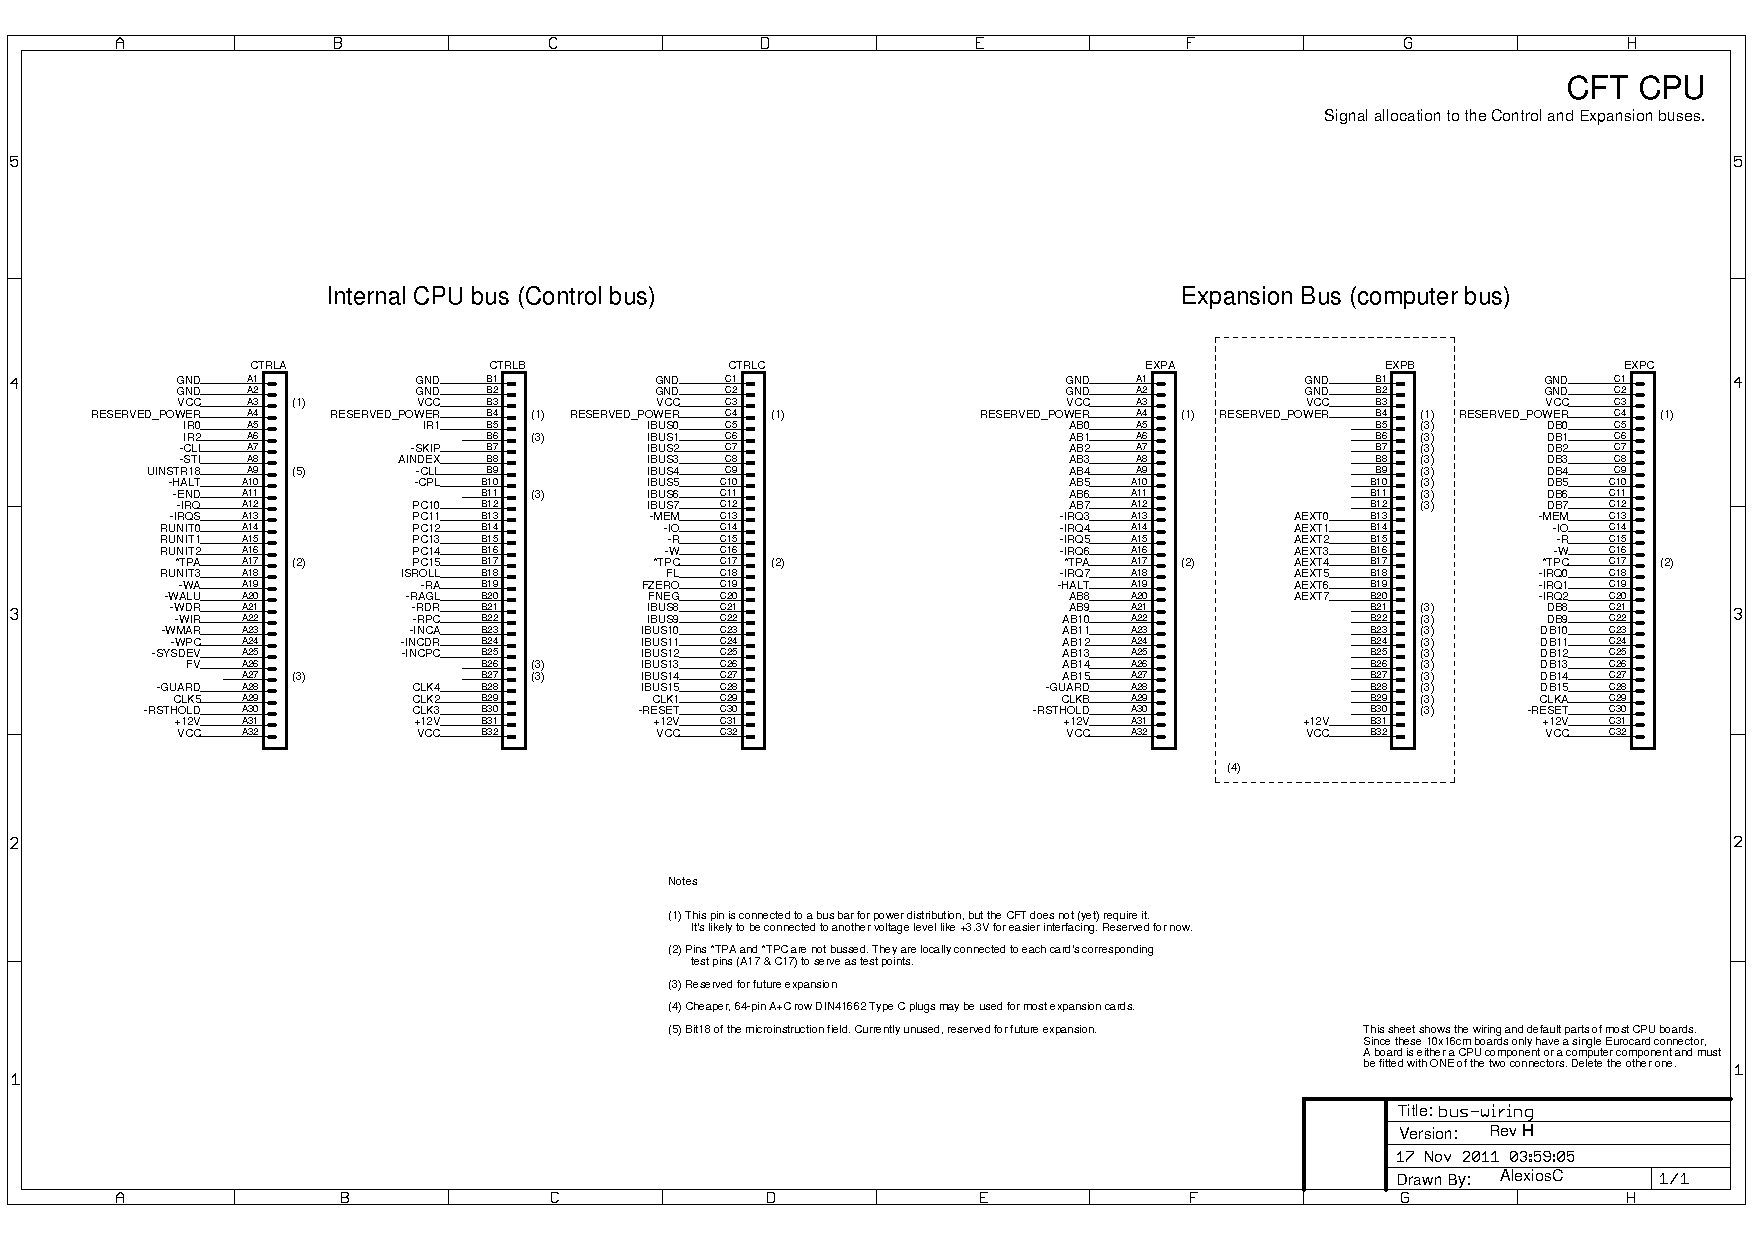
\includegraphics[width=0.95\textheight,angle=90]{figs/bus-wiring.pdf}\\
%% \caption{\label{fig-schematic-bus-wiring}Schematic drawing of the bus wiring.}
%% \end{figure*}


%%  LocalWords:  documentclass CFT Alexios PDP autoindexing Von LSI Chouchoulas
%%  LocalWords:  Neumann microprograms microprogram microinstructions Bauform
%%  LocalWords:  et cetera kiloword KWord kilowords KWords Autoindex rp GND CLC
%%  LocalWords:  SUBRET JSR TRAPRET ISRRET ISR autoindex th FC FFF tl RSTIN tri
%%  LocalWords:  FFFF pagerel vlgrey linewidth fillstyle fillcolor de GPULSE
%%  LocalWords:  addr FFFE IOT LIA JMP bitwise ORred asm bitfield CLA DMA IRQ
%%  LocalWords:  CLL RBL RBR RNL RNR NOP linearc SNA SZA SSL SNN SNZ
%%  LocalWords:  SCL CLI STI SNP lll RET RTT SBL SBR SNL SNR TTY
%%  LocalWords:  disjuncted conjuncted ANDed

  
  \chapter{Microcode}
  \glsresetall
  \label{chap:microcode}
  %% This chapter describes the CFT Microcode.

\section{Microcode Theory}

Dieter Müller (Mueller) has a very useful resource on understanding
and writing microcode, and it's suitable for beginners in the
art. It's available at
\url{http://6502.org/users/dieter/mpd/mpd_0.htm}. It forms a very good
introductory document.

Microcode formats are usually split into three major groups:

%% \begin{itemize}
%%   \item{\bfseries Vertical Microcode}, where each micro-instruction is
%%     decoded by the control unit before being able to drive control
%%     signals. Vertical microcode is very compact but requires
%%     additional decoding circuitry (and time).
%%   \item{\bfseries Horizontal Microcode}, where each control signal is
%%     directly encoded in the micro-instruction. Horizontal microcode
%%     formats tend to be extremely wide, but they do not need decoding.
%%   \item{\bfseries Hybrid Formats}, where parts are horizontal and
%%     parts are vertical.
%% \end{itemize}

CFT Microcode is hybrid. A number of fields in the format are
vertically encoded to save bits, but also to avoid bus contention
issues. Consider horizontal microcode to select which unit to enable
for reading from:

%% \begin{center}
%%   \zebra
%%   \begin{tabular}{*{3}{c>{\textsf\bgroup}c<{\egroup}}l}
%%     %\noalign{\smallskip}\hline\noalign{\smallskip}
%%     %\\\hline
%%     A & B & C & Read from\\
%%     %\noalign{\smallskip}\hline\noalign{\smallskip}
%%     \hline
%%     H & H & H & Nothing (all units idle)\\
%%     L & X & X & Unit A\\
%%     X & L & X & Unit B\\
%%     X & X & L & Unit C\\
%%     L & L & L & \textrm{\bfseries Fault: all units (bus contention).}\\
%%     \hline
%%   \end{tabular}
%% \end{center}

The first four cases are valid cases of microcode use. The fourth one,
however, represents one of four cases where multiple units are enabled
for read, causing bus contention and possibly damage to the
processor. This way of storing this information is also highly
wasteful: three bits are used to store four different valid states,
which only uses 50\% of the range afforded by three bits ($2^3 = 8$).

A better case, which completely eliminates the contention issue, is to
encode these bits vertically:

%% \begin{center}
%%   \zebra
%%   \begin{tabular}{*{1}{>{\textsf\bgroup}c<{\egroup}}l}
%%     %\noalign{\smallskip}\hline\noalign{\smallskip}
%%     %\\\hline
%%     SRC & Read from\\
%%     %\noalign{\smallskip}\hline\noalign{\smallskip}
%%     \hline
%%     00 & Nothing (all units idle)\\
%%     01 & Unit A\\
%%     10 & Unit B\\
%%     11 & Unit C\\
%%     \hline
%%   \end{tabular}
%% \end{center}

This format saves one bit, and removes invalid or dangerous
states. This technique is used on the CFT in exactly this way and for
exactly this reason.


\section{The Microcode Assembler}

Most microcode formats are usually assembled using helper software of
various types.  The CFT microcode was prepared using \texttt{mcasm}, a
Microcode Assembler written for this express task, but probably of use
in other similar tasks. The assembler is available online at:

\begin{center}
  \url{http://www.bedroomlan.org/projects/mcasm}
\end{center}

It is written in the Python programming language.\footnote{Itself available at
  \url{http://python.org}, though most modern operating systems bundle it.} The
assembler provides macro and preprocessing facilities using the GNU C
Preprocessor, which is provided with the free GNU C Compiler. Its syntax
borrows numerous elements from C, so it can co-operate with the C
Pre-processor, and so that editor systems can recognise enough of it to provide
syntax highlighting.

The macro facilities allow common tasks like memory cycles to be repeated
without the possibility of minor errors that could introduce processor bugs.

The assembler is capable of providing diagnostic output about the quality of
the code, and generates binary images of as many ROMs as are required to store
the wide micro-instructions.


\begin{figure}
  \centering
  \inputfigure{figure-microcode-store}

  \caption[Microcode structure]{\label{fig:microcode-store2}Microcode
    structure. The Address or Conditional Vector (top) is an input to
    the microcode store. The control vector (bottom) is the Microcode
    store's output. It drives the processor's units. }
\end{figure}


\section{Microcode Address Vector}

The processor's microcode is functionally similar to the cam timer in an
old-style washing machine, or the cylinder of a music box. A program is
executed one step at a time. Each step, one or more units are activated. A
washing machine's cam timer controls the various devices in the washing machine
as a function of time. A music box uses studs to trigger musical instruments as
a function of time.

The microcode could also be visualised as a long table, each column of which
controls one or more units.

The main difference is that the current position in the microcode can jump from
one place to the next. This is a form of flow control.

The CFT microcode has a composite microcode address formed of a number of {\em
  conditionals\/} (in \texttt{mcasm} terminology). This information is also
available in~\cf{sec:microcode-format} and illustrated
in~\fcf{fig:microcode-store2}. In short, the address is a vector of ten fields:

\begin{description}
\item \textbf{Bits 0–3: \UPC}. This is the output of the microcode counter as
  described in~\cf{sec:upc} and represents the offset inside a
  microprogram. The remainder of the bits identify different microprograms.
\item \textbf{Bit 4: \ns{AINDEX}}. Asserted by the Autoindex Logic when autoindex memory locations are accessed. The Autoindex Logic is described in~\cf{sec:ail}.
\item \textbf{Bit 5: \ns{SKIP}}. Asserted by the Skip logic when a microcode
  branch must be performed. One side of the branch may affect flow control at
  the processor level, by appropriate manipulation of the \PC. This is perhaps the most complex and powerful microcode operation. It is discussed in~\cf{sec:sbu}.
\item \textbf{Bit 6: \IRn{11}}. This is R field of instructions, as discussed
  in~\cf{sec:instruction-format}.
\item \textbf{Bits 7–10: \IRn{12–15}}. This is the opcode of the currently
  executing instruction, as discussed in~\cf{sec:instruction-format}.
\item \textbf{Bit 11: \ps{FL}}. The current value of the \Lreg.
\item \textbf{Bit 12: \ps{FV}}. The current value of the overflow flag.
\item \textbf{Bit 13: \ns{IRQS}}. Asserted if interrupts are allowed, an
  interrupt has been received, and a new instruction has just started
  fetching. The signal remains asserted for the duration of the microprogram,
  which is conventionally the microprogram that induces the processor to jump
  to the \gls{Interrupt Service Routine}. This is discussed in detail
  in~\cf{sec:interrupts-state-machine}.
\item \textbf{Bit 14: \ns{RSTHOLD}}. Asserted for a set number of clock cycles after a reset. Used to run the reset microprogram, which initialises certain registers.
\item \textbf{Bits 15–19: \UCB}. This is an optional extension to the microcode
  store. It identifies the microcode bank being used. Each microcode bank
  contains the full microcode of the CFT, with variations allowing for
  different machine revisions to be implemented, or extending the instruction
  set. These bits are normally \bin{0000}. This is discussed in~\cf{sec:ucb}
\end{description}


\section{Microprogram structure}

The microcode store is split into a number of microprograms, each allocated 16
Instructions. The \UPC{} acts as the program counter {\em within\/} a
microprogram, while the remainder of the address vector selects which
microprogram is executed.

Microprograms are prioritised: when the computer is being reset, the value of
the \IR{} is immaterial. If the computer is executing a \asm{LOAD} instruction,
the value of the \ns{SKIP} component of the address vector is immaterial. These
don't-care values are illustrated in~\tcf{table:microprograms}:

%%     \zebrarow{10}
%%     \begin{longtable}{*{8}{>{\textsf\bgroup}c<{\egroup}}l}
%%       %
%%       % First header
%%       %
%%     \hiderowcolors
%%     \ns{RSTHOLD} & \ns{IRQS} & \ps{FV} & \ps{FL} & \IRn{12–15} & \IRn{11} & \ns{SKIP} & \ns{AINDEX} & Microprogram \\
%%     \hline
%%     \noalign{\global\rownum 0\relax}\showrowcolors
%%     \endfirsthead
%%     %
%%     % Subsequent headers
%%     %
%%     \hiderowcolors
%%     \noalign{\smallskip\smallskip}
%%     \multicolumn{9}{l}{\em Continued from previous page.}\\
%%     \ns{RSTHOLD} & \ns{IRQS} & \ps{FV} & \ps{FL} & \IRn{12–15} & \IRn{11} & \ns{SKIP} & \ns{AINDEX} & Microprogram \\
%%     \hline
%%     \noalign{\global\rownum 1\relax}\showrowcolors
%%     \endhead
%%     %
%%     % Footer
%%     %
%%     \hiderowcolors
%%     \hline
%%     \noalign{\smallskip\smallskip}
%%     \multicolumn{9}{l}{\em Continued on next page.}\\
%%     \endfoot
%%     %
%%     % Last footer
%%     %
%%     \hiderowcolors
%%     \hline
%%     \endlastfoot
%%     %
%%     % Content
%%     %
%%     \showrowcolors
%%     L & X & X & X & X & X & X & X & Reset processor\\
%%     H & L & X & X & X & X & X & X & Interrupt handler\\
%%     %
%%     H & H & X & X & \bin{0000} & \bin{0} & X & H & \asm{TRAP} Direct \\
%%     H & H & X & X & \bin{0000} & \bin{1} & X & H & \asm{TRAP} Indirect \\
%%     H & H & X & X & \bin{0000} & \bin{1} & X & L & \asm{TRAP} Autoindex \\
%%     %
%%     H & H & X & X & \bin{0001} & \bin{0} & X & H & \asm{IOT} Direct \\
%%     H & H & X & X & \bin{0001} & \bin{1} & X & H & \asm{IOT} Indirect \\
%%     H & H & X & X & \bin{0001} & \bin{1} & X & L & \asm{IOT} Autoindex \\
%%     %
%%     H & H & X & X & \bin{0010} & \bin{0} & X & H & \asm{LOAD} Direct \\
%%     H & H & X & X & \bin{0010} & \bin{1} & X & H & \asm{LOAD} Indirect \\
%%     H & H & X & X & \bin{0010} & \bin{1} & X & L & \asm{LOAD} Autoindex \\
%%     %
%%     H & H & X & X & \bin{0011} & \bin{0} & X & H & \asm{STORE} Direct \\
%%     H & H & X & X & \bin{0011} & \bin{1} & X & H & \asm{STORE} Indirect \\
%%     H & H & X & X & \bin{0011} & \bin{1} & X & L & \asm{STORE} Autoindex \\
%%     %
%%     H & H & X & X & \bin{0100} & \bin{0} & X & H & \asm{IN} Direct \\
%%     H & H & X & X & \bin{0100} & \bin{1} & X & H & \asm{IN} Indirect \\
%%     H & H & X & X & \bin{0100} & \bin{1} & X & L & \asm{IN} Autoindex \\
%%     %
%%     H & H & X & X & \bin{0101} & \bin{0} & X & H & \asm{OUT} Direct \\
%%     H & H & X & X & \bin{0101} & \bin{1} & X & H & \asm{OUT} Indirect \\
%%     H & H & X & X & \bin{0101} & \bin{1} & X & L & \asm{OUT} Autoindex \\
%%     %
%%     H & H & X & X & \bin{0110} & \bin{0} & X & H & \asm{JMP} Direct \\
%%     H & H & X & X & \bin{0110} & \bin{1} & X & H & \asm{JMP} Indirect \\
%%     H & H & X & X & \bin{0110} & \bin{1} & X & L & \asm{JMP} Autoindex \\
%%     %
%%     H & H & X & X & \bin{0111} & \bin{0} & X & H & \asm{JSR} Direct \\
%%     H & H & X & X & \bin{0111} & \bin{1} & X & H & \asm{JSR} Indirect \\
%%     H & H & X & X & \bin{0111} & \bin{1} & X & L & \asm{JSR} Autoindex \\
%%     %
%%     H & H & X & X & \bin{1000} & \bin{0} & X & H & \asm{ADD} Direct \\
%%     H & H & X & X & \bin{1000} & \bin{1} & X & H & \asm{ADD} Indirect \\
%%     H & H & X & X & \bin{1000} & \bin{1} & X & L & \asm{ADD} Autoindex \\
%%     %
%%     H & H & X & X & \bin{1001} & \bin{0} & X & H & \asm{AND} Direct \\
%%     H & H & X & X & \bin{1001} & \bin{1} & X & H & \asm{AND} Indirect \\
%%     H & H & X & X & \bin{1001} & \bin{1} & X & L & \asm{AND} Autoindex \\
%%     %
%%     H & H & X & X & \bin{1010} & \bin{0} & X & H & \asm{OR} Direct \\
%%     H & H & X & X & \bin{1010} & \bin{1} & X & H & \asm{OR} Indirect \\
%%     H & H & X & X & \bin{1010} & \bin{1} & X & L & \asm{OR} Autoindex \\
%%     %
%%     H & H & X & X & \bin{1011} & \bin{0} & X & H & \asm{XOR} Direct \\
%%     H & H & X & X & \bin{1011} & \bin{1} & X & H & \asm{XOR} Indirect \\
%%     H & H & X & X & \bin{1011} & \bin{1} & X & L & \asm{XOR} Autoindex \\
%%     %
%%     H & H & X & X & \bin{1100} & \bin{0} & H & H & \asm{OP1} Direct, \asm{NOP}s \\
%%     H & H & X & X & \bin{1100} & \bin{1} & L & H & \asm{OP1} Indirect, actions \\
%%     %
%%     H & H & X & X & \bin{1101} & \bin{0} & H & H & \asm{OP2} Direct, \asm{NOP}s \\
%%     H & H & X & X & \bin{1101} & \bin{1} & L & H & \asm{OP2} Indirect, actions \\
%%     %
%%     H & H & X & X & \bin{1110} & \bin{0} & H & H & \asm{ISZ} Direct, no skip \\
%%     H & H & X & X & \bin{1110} & \bin{0} & L & H & \asm{ISZ} Direct, skip \\
%%     H & H & X & X & \bin{1110} & \bin{1} & H & H & \asm{ISZ} Indirect, no skip \\
%%     H & H & X & X & \bin{1110} & \bin{1} & L & H & \asm{ISZ} Indirect, skip \\
%%     H & H & X & X & \bin{1110} & \bin{1} & H & L & \asm{ISZ} Autoindex, no skip \\
%%     H & H & X & X & \bin{1110} & \bin{1} & L & L & \asm{ISZ} Autoindex, skip \\
%%     %
%%     H & H & X & X & \bin{1111} &       X & X & X & \asm{LIA} Immediate \\
%%   \end{longtable}

%%   %% \caption[Table of microprograms]{\label{table:microprograms}Table of
%%   %%   microprograms in the Microprogram Store.}

The don't-care (partial address decoding) values indicate that exactly
half of the microprograms are ‘Reset’ microprograms, one quarter are
‘Interrupt handler’ microprograms, and even many instructions exist in
multiple copies in the microcode store.

\section{Microcode Control Vector}

This information is also available in~\cf{sec:microcode-format}, and
illustrated in~\fcf{fig:microcode-store2}.


\begin{description}
\item \textbf{Bits 0–3: \RUNITn{0–3}}. Vertical field, identifies the processor
  unit to read from, and includes \ALU operations and constants which are ‘read’
  from as if they were separate units operating in tandem.
\item \textbf{Bits 4–6: \WUNITn{0–2}}. Vertical field, identifies the processor unit to write to.
\item \textbf{Bits 7–10: \OPIFn{0–3}}. Vertical field, identifies an
  instruction register bit whose value is routed to the next
  micro-instruction's \ns{SKIP} input.
\item \textbf{Bit 11: \CLL}. Clears \Lreg.
\item \textbf{Bit 12: \CPL}. Complements \Lreg.
\item \textbf{Bit 13: \STI}. Allows interrupts.
\item \textbf{Bit 14: \CLI}. Masks interrupts.
\item \textbf{Bit 15: \INCPC}. Increments \PC.
\item \textbf{Bit 16: \STPDR}. Steps the \DR register.
\item \textbf{Bit 17: \STPAC}. Steps the \AC register.
\item \textbf{Bit 18: \DEC}. When this signal is asserted, \STPDR{}
  and \STPAC{} decrement the \DR{} and \AC{} registers
  respectively. At other times, \STPDR{} and \STPAC{} increment \DR{}
  and \AC{}.
\item \textbf{Bit 19: \MEM}. Indicates a memory cycle.
\item \textbf{Bit 20: \IO}. Indicates an I/O cycle.
\item \textbf{Bit 21: \R}. Indicates a read cycle.
\item \textbf{Bit 22: \WEN}. Indicates a write cycle.
\item \textbf{Bit 23: \END}. Ends the current microprogram.
\end{description}





\section{Microcode State Transitions}

In digital circuits, glitches are short state changes that happen when a
circuit's inputs are moving from one state to another. One benefit of using a
memory chip-based microcode store rather than combinatorial logic is that these
glitches are largely removed.

The potential glitches remaining are logical: as the address vector
changes from one value to another, the values of the outputs must
remain sane.

The state changes of the microcode represent and implement the state
changes of the processor, as described in~\cf{sec:major-states}. Wait
states are not handled by the microcode engine. They cause it to be
suspended temporarily, but this is done by inhibiting \UPC{}
increments and the microcode store is unaware of this. A number of
additional, minor states are accommodated by the microcode: addressing
modes and flow control are the major examples of this.

\subsection{Resetting}

When the \ns{RSTHOLD} conditional is asserted, the microcode address jumps
directly to the {\em middle\/} of the reset microprogram, with the
\UPC{} not reset at all. The reset microprogram is a very simple
affair, however. All it does is load the \PC{} and signal a
microprogram end. This resets the \UPC{}, starting the program over
from the beginning until \ns{RSTHOLD} is cleared.

At that point, the microprogram exits, with the \PC{} appropriately
initialised and the \UPC{} cleared. The next micro-program will be an
instruction fetch for an arbitrary (don't-care) instruction, although
this instruction will always be \bin{0000} (\asm{TRAP}) since the
\IR{} will have been reset to \hex{0000} by the \ns{RESET} signal.

\subsection{Interrupt Handling}

When the \ns{INT} conditional is asserted, the microcode address jumps
directly to the interrupt handler microprogram. Since the \UPC{} is
not affected by this, this would be the middle of the micro-program,
but external registration circuitry ensures that \ns{INT} is only ever
asserted when \UPC{} is zero.

Thus, interrupts are serviced after the end of the previous
instruction and never while carrying it out.

The interrupt handler's first action is to clear interrupts, which
also clears the \ns{INT} conditional. This action is also registered
and is detected by the microcode store at the end of the interrupt
handler microprogram, when \ns{END} is asserted and \UPC{} is reset to
zero. At that point, the interrupt handler microprogram exits and a
new instruction is fetched. (which, since the \PC{} has been set to the
\abbr{ISR} vector, will belong to the macro-program interrupt service
routine)

\subsection{Fetching an Instruction}

The first micro-program cycles of every normal instruction
micro-program contain copies of the exact same fetch microcode. This
code loads the \IR{} from memory, using the current value of the
\PC{}, then increments the \PC{} by one.

The action of loading the \IR{} causes a jump from whatever
instruction's micro-program is executing to a new one. The first
micro-instruction after the end of the fetch cycle begins execution of
the instruction just loaded.

\subsection{Flow Control}

For the most part, the skip logic is idle, which causes \ns{SKIP} to
stay high. Should a micro-instruction request a test of a flag, the
\ns{SKIP} line may be asserted, which will immediately cause a
microprogram jump to a new, non-contiguous address. That address
should perform actions to take skip actions, usually asserting
\ns{INCPC} to increment the \PC{}.

In the next micro-instruction, the \ns{SKIP} conditional will revert
to de-asserted, causing another jump back to the non-skipping version
of the micro-program.

Skipping and non-skipping micro-programs are thus exactly the same
length. Where necessary, this is done by not doing anything, which
causes branching and non-branching instructions to take the same time
to run. This is unusual, since many processors require one less clock
cycle if the branch is not taken. In the case of the CFT, this is less
important since branching is performed by the \asm{OP2} instruction
with performs other optional tasks after the branch (regardless of
whether the branch is taken or not).

It is obvious that flow control happens by jumping from one
micro-program to another without modifying the \UPC{}. This allows
different microcode to be executed. All flow control is performed
using the \OPIF{} microcode field, and affects the microcode
only. Instruction-level flow control is observed as a side-effect of
microcode flow control: simply put, to take an Assembly-level skip,
microcode needs to increment the \PC{}. To not take a skip, the
microcode needs to do nothing.

\subsection{Negative and Overflow skips}

The microcode ROM had a few spare address pins, and these were
connected to the negative and overflow flag registers to allow for
some unforeseen skip instructions. This allowed the \asm{IFV} and
\asm{IFN} sub-instructions to be coded.

These are handled and behave in a way almost identical to that of the
\ns{SKIP} conditional. The unfortunate side effect is that
microprograms that handle both flag conditionals need to be coded four
times, one for each combination of the two flags.

\subsection{Indirection}

Indirect mode is selected by setting \IRn{11}. This is loaded at fetch
time, and is not modified during microprogram execution. Thus, it
works in conjunction with \IRn{12–15} to select among 16 direct and 16
indirect instruction micro-programs (autoindex mode is a variation of
indirect mode).

Instructions \asm{OP1}, \asm{OP2} and \asm{LIA} treat this as a don't
care value, so there are double as many copies of each micro-program
for these instructions.

Indirect mode is updated at the end of the fetch cycle, causing a jump
to the appropriate direct or indirect (or don't care) micro-program.

\subsection{Autoindexing}

Asserting the \ns{AINDEX} conditional causes a jump to the autoindex
versions of instruction microprograms. When \IRn{11} is clear (direct
mode), \ns{AINDEX} is treated as a don't-care value, so is
immaterial. When \IR{11} is set (high), indirect mode is
active. Autoindexing works in indirect mode by executing additional
code at the end of the instruction execution micro-program.

The \ns{AINDEX} conditional is latched based on the value of the
\AR{}. Once set, it remains set until the end of the microprogram,
avoding jumps back to the non-autoindex code. This is necessary since
the \AR{} changes during execution and its new value is likely to
cancel \ns{AINDEX} mid-instruction.

Instructions that observe autoindex mode behave like their indirect
mode versions. At the end of the instruction, additional code
increments the memory location identifyed by the instruction operand.

The microcode sequencer contains a flaw-like limitation to keep
circuitry simple: if an indirect-mode instruction is fetched from an
address in the range \hex{0080}–\hex{00FF} and the previous address
was also an indirect-mode instruction, autoindex mode will be set
regardless of the newly fetched instruction's operand. This is
considered an acceptable limitation, as the autoindex locations are a
limited, highly useful resource, and there is no good reason to be
executing code there.

\subsection{Unusual Glitches}

To avoid unusual glitches, every unused location of the microcode
store asserts \ns{END}, which causes the microprogram to reset. This
should never happen, but if it does, it ensures the processor will
carry on with the next instruction.

\section{Microcode Listing}

\todo{Reinstate the listing.}


%% %{\small
%% \lstinputlisting[style=longmcasm]{../../../microcode/microcode.mc}
%% %}

  
  \chapter{Processor Schematics}
  \glsresetall
  \label{chap:processor-schematics}
  
The following page shows the full schematic drawings of the three processor boards.

\cleardoublepage
\phantomsection\stepcounter{section}%
\addcontentsline{toc}{section}{\protect\numberline{\thesection} Processor Board A Schematics}

\includeschns{2}{Clock Generation and control}{sch:clock}
\includeschns{3}{Reset Handling and Sequencing}{sch:reset}
\includeschns{4}{Microcode Sequencer}{sch:useq}
\includeschns{5}{Microcode Sequencer Signal Hold}{sch:useq-hold}
\includeschns{7}{Read and Write Unit Decoding}{sch:unit-decoders}
\includeschns{8}{Skip and Branch Logic}{sch:sbu}
\includeschns{9}{Address Generation Logic}{sch:agl}
\includeschns{10}{Instruction Register}{sch:ir}
\includeschns{11}{Interrupt State Machine}{sch:intsm}
\includeschns{12}{Data Bus Driver and Bus Termination}{sch:databus}
\includeschns{6}{Microcode Sequencer Front Panel Buffers and Connectors}{sch:useq-fp}

\phantomsection\stepcounter{section}%
\addcontentsline{toc}{section}{\protect\numberline{\thesection} Processor Board B Schematics}

\includeschns{13}{Address Register, Address Bus Drivers \& Termination, Autoindex Logic and Device Decoder}{sch:ar}
\includeschns{14}{Program Counter}{sch:pc}
\includeschns{15}{Data Register}{sch:dr}
\includeschns{16}{Accumulator, Zero Flag and Negative Flag}{sch:ac}

\phantomsection\stepcounter{section}%
\addcontentsline{toc}{section}{\protect\numberline{\thesection} Processor Board C Schematics}

\includeschns{17}{Link Register}{sch:l}
\includeschns{18}{Arithmetic/Logic Unit: Decoders and Buffers}{sch:aludecoder}
\includeschns{19}{ALU Binary Operators}{sch:alub}
\includeschns{20}{ALU Unary Operators and Constant Store}{sch:aluu}
\includeschns{21}{8 kW Bank Switching Memory Controller}{sch:mbu}

\fi

\ifdefined\renderpartperipherals
\part{Peripherals}
  \ifdefined\renderchappfp
    \chapter{Front Panel}
    \glsresetall
    \documentclass[11pt,a4paper,twocolumns]{article}
\usepackage[all]{xy}
\usepackage{tikz-timing}[2009/07/28]
\usetikztiminglibrary{either}[2009/07/28]
\usepackage{pdftricks}
\usepackage{epsfig}
\usepackage{lipsum}
\usepackage{float}
\usepackage{verbatim}
\usepackage{geometry}
\usepackage{graphicx}
\usepackage{color}
\usepackage{epic}
\usepackage{eepic}
\usepackage{fontspec}
\usepackage[dvipdfm,a4paper,CJKbookmarks,bookmarks=true,bookmarksopen=true]{hyperref}
\usepackage{longtable}
\begin{psinputs}
\usepackage{color}
\usepackage{longtable}
\usepackage{pstcol}
\usepackage{pstricks}
\usepackage{pst-plot}
\usepackage{pst-tree}
\usepackage{pst-eps}
\usepackage{multido}
\usepackage{pst-node}
\usepackage{pst-eps}
\end{psinputs}
\definecolor{darkblue}{RGB}{0,0,128}
\hypersetup{
    pdftitle={CFT Minicomputer Front Panel Operations},
    pdfauthor={Alexios Chouchoulas},
    pdfkeywords={},
    bookmarksnumbered,
    pagebackref=true,
    breaklinks=true,
%    pdfview=FitH,       % Or try pdfstartview={FitV}, This lead to uncorrect bookmarks
    urlcolor=darkblue,
    colorlinks=true,
    citecolor=blue,          %citeref's color
    linkcolor=blue,
        }
% Fonts
%\defaultfontfeatures{Mapping=tex-text}
\setmainfont{Minion Pro}
\setsansfont{Myriad Pro}
\setmonofont[]{Inconsolata}

%\renewcommand{\rmdefault}{put}

\geometry{a4paper, hoffset=0in, voffset=-.25in, left=1.5cm, right=1.5cm,
  top=2.5cm, bottom=2.5cm}
\sloppy

% Use hyperlinking when renderind PDFs
\newcommand{\cf}[2][section]{\hyperref[#2]{#1 \ref*{#2} (p.~\pageref*{#2})}}
\newcommand{\npcf}[2][section]{\hyperref[#2]{#1 \ref*{#2}}}
\newcommand{\appcf}[1]{\cf[appendix]{#1}}
\newcommand{\ccf}[1]{\cf[chapter]{#1}}
\newcommand{\fcf}[1]{\cf[figure]{#1}}
\newcommand{\tcf}[1]{\cf[table]{#1}}
\newcommand{\ecf}[1]{\cf[equation]{#1}}
\newcommand{\algcf}[1]{\cf[algorithm]{#1}}
\newcommand{\npappcf}[1]{\npcf[appendix]{#1}}
\newcommand{\npccf}[1]{\npcf[chapter]{#1}}
\newcommand{\npfcf}[1]{\npcf[figure]{#1}}
\newcommand{\nptcf}[1]{\npcf[table]{#1}}
\newcommand{\npecf}[1]{\npcf[equation]{#1}}
\newcommand{\npalgcf}[1]{\npcf[algorithm]{#1}}

\setlength\columnsep{7mm}

\newcommand\hyperemail[1]{\sf\href{mailto:#1}{#1}}
\newcommand\link[1]{\sf\href{http://#1}{#1}}

\newcommand{\ns}[1]{$\overline{\mbox{\textsf{{#1}}}}$}
\newcommand{\ps}[1]{\textsf{#1}}
\newcommand{\lt}[1]{\textsf{#1}}
\newcommand{\sw}[1]{\textsf{#1}}

\newcommand{\schpt}[1]{\textsf{#1}}

\newcommand\bus[1]{{#1}}
\newcommand\unit[1]{{#1}}
\newcommand\IBUS{\bus{IBUS}}
\newcommand\ALU{\unit{ALU}}
\newcommand\SBU{\unit{SBU}}
\newcommand\AGL{\unit{AGL}}
\newcommand\register[1]{\textsf{#1}}
\newcommand\A{\register{AC}}
\newcommand\AC{\A}
\newcommand\Lreg{\register{L}}
\newcommand\Ireg{\register{I}}
\newcommand\MAR{\register{MAR}}
\newcommand\DR{\register{DR}}
\newcommand\PC{\register{PC}}
\newcommand\IR{\register{IR}}

\newcommand\UINSTR{\ns{uINSTR18}}
\newcommand\HALT{\ns{HALT}}
\newcommand\END{\ns{END}}
\newcommand\IRQ{\ns{IRQ}}
\newcommand\IRQS{\ns{IRQS}}
\newcommand\IRQn[1]{\ns{IRQ{#1}}}
\newcommand\RUNITn[1]{\ps{RUNIT{#1}}}
\newcommand\TPA{\ps{TPA}}
\newcommand\TPC{\ps{TPC}}
\newcommand\WAC{\ns{WAC}}
\newcommand\WALU{\ns{WALU}}
\newcommand\WDR{\ns{WDR}}
\newcommand\WIR{\ns{WIR}}
\newcommand\WMAR{\ns{WMAR}}
\newcommand\WPC{\ns{WPC}}
\newcommand\SYSDEV{\ns{SYSDEV}}
\newcommand\OPIFn[1]{\ps{OPIF{#1}}}
\newcommand\GUARDPULSE{\ns{GUARD}}
\newcommand\GP{\GUARDPULSE}
\newcommand\CLOCK[1]{\ps{CLK{#1}}}
\newcommand\RSTHOLD{\ns{RSTHOLD}}
\newcommand\BOE{\ns{BOE}}
\newcommand\UOE{\ns{UOE}}
\newcommand\SKIP{\ns{SKIP}}
\newcommand\AINDEX{\ps{AINDEX}}
\newcommand\CLL{\ns{CLL}}
\newcommand\CPL{\ns{CPL}}
\newcommand\CLI{\ns{CLI}}
\newcommand\STI{\ns{STI}}
\newcommand\IRn[1]{\ps{IR{#1}}}
\newcommand\PCn[1]{\ps{PC{#1}}}
\newcommand\IBUSn[1]{\ps{IBUS#1}}
\newcommand\DBUSn[1]{\ps{DB#1}}
\newcommand\ABUSn[1]{\ps{AB#1}}
\newcommand\AEXTn[1]{\ps{AEXT#1}}
\newcommand\ISROLL{\ps{ISROLL}}
\newcommand\RAC{\ns{RAC}}
\newcommand\RAGL{\ns{RAGL}}
\newcommand\RDR{\ns{RDR}}
\newcommand\RPC{\ns{RPC}}
\newcommand\INCAC{\ns{INCAC}}
\newcommand\INCDR{\ns{INCDR}}
\newcommand\INCPC{\ns{INCPC}}
\newcommand\MEM{\ns{MEM}}
\newcommand\IO{\ns{IO}}
\newcommand\R{\ns{R}}
\newcommand\WRITE{\ns{W}}
\newcommand\READ{\ns{R}}
\newcommand\FL{\ps{FL}}
\newcommand\FV{\ps{FV}}
\newcommand\FZERO{\ps{FZERO}}
\newcommand\FNEG{\ps{FNEG}}
\newcommand\RESET{\ns{RESET}}

\newcommand\NB{\textbf{Nota Bene:\ }}

\begin{document}
\thispagestyle{empty}
\pagestyle{plain}
\twocolumn[
\centering

\includegraphics{figs/cft-logo-v1.pdf}\vspace{2em}\\
{\LARGE\bf CFT Minicomputer Front Panel Operation}
\vspace{10pt}

{\Large Alexios Chouchoulas}\\\vspace{5pt}
{\large \hyperemail{alexios@bedroomlan.org}}

\vspace{20pt}

\begin{minipage}{.75\textwidth}
  \begin{abstract}
    \small
    
  This document discusses tentative design and implementational
  details of the CFT computer's front panel and its intended
  operation. The front panel was designed last but is meant to be
  built first to aid in building, testing and operating the CFT
  computer during and after its construction. It also provides a
  traditional minicomputer programming interface, albeit a modernised
  LED-based one.
    
  \end{abstract}
  
  \section*{History of Changes}
  \small

  {\bf 2011-12-19} Initial revision.

  {\bf 2012-01-04} Listed briefly the signal connections between front
  panel and processor boards.

  \vspace{5ex}
  
\end{minipage}
] % End of \twocolumn
\section{Introduction}

The CFT minicomputer is intended to be similar to a 1960s
minicomputer, and it could never be similar enough without a
programmer's front panel.

The front panel is serves two purposes: to inspect the state of the
computer, and to modify the state of the computer. State inspection is
made possible via a number of lights corresponding to the binary state
of most of the computer's crucial signals. State modification is via a
number of switches which control the operation of the computer's main
units and provide user input.

The CFT front panel is expected to provide a number of services.

\begin{itemize}
\item During construction, it will provide a means of testing most of
  the computer's individual units on their own. With some rewiring or
  reconfiguration, all of the computer's features can be tested.

\item After construction, it will allow microcode to be inspected and
  thereby debugged.

\item It will also allow the computer to be programmed without a
  ROM. A front panel was usually the only built-in means of
  programming a minicomputer, and in many cases was the only way the
  computer could be booted up.

\item It will allow debugging of software and hardware by allowing the
  computer to be stopped, its state inspected and perhaps changed, and
  then resuming execution.

\item Finally, it will allow the state of the running computer to be
  inspected with varying degrees of success.\footnote{The human eye
    is, of course, incapable of registering light pulses with MHz
    frequencies, but the panel lights register these with varying
    intensities of light.}

\end{itemize}

\section{Layout of the Front Panel}

\begin{figure*}[t]
\centering
\includegraphics[width=\textwidth]{../../panel/front-panel-v2-small.jpg}\\
\caption{\label{fig-panel}A first draft of the CFT front panel.}
\end{figure*}

The CFT minicomputer is intended to be built into a 19-inch rack-mount case, 6U
in height, making it approximately 19" by 10.5" (482.6mm by 266.7mm) in size.

The panel displays the state of the computer on 118 console lights. For lower
consumption, convenience and longevity, these are light-emitting diodes (LEDs).

30 toggle switches allow the computer's state to be modified, and user input to
be provided.

Computer power and panel locking is controlled by a three-position key switch.

All lights and switches are displaying multi-bit quantities are arranged with
the most significant bit to the right, in the conventional notation of binary
numbers. Bit numbers start at 0, which is the least significant bit or
rightmost light. This follows the conventional notation of powers-of-two.

\subsection{Console Lights}

The console lights are arranged in six rows.

\subsubsection{Memory Controller}

The leftmost bank of lights on the top row displays the status of the banking
memory controller, if it is installed.

If banking has been enabled, a green light marked \lt{ENABLED} indicates
this. Eight yellow lights marked \lt{AEXT7}–\lt{AEXT0} indicate the bank
currently selected.

Conventionally, the memory controller addresses up to one MWord of ROM mapped
in the top MWord of the 21-bit address space (physical addresses {\sf
  20:0000}–{\sf 3F:FFFF}). Thus, light \lt{AEXT7} also indicates that a ROM
bank is selected. The light is thus marked \lt{AEXT7/ROM}).

If the memory controller board is not installed, these lights remain off.

\subsubsection{Interrupt Controller}

The middle bank of lights on the top row indicates the status of the optional
interrupt controller on eight lights marked \lt{INT7}–\lt{INT0}.

Each of these lights will indicate a number of different conditions depending
on its colour.

\begin{itemize}
  \item {\bf Off}: the computer is ignoring this interrupt line, and there is
    no interrupt activity.
  \item {\bf Green}: the interrupt line is being used by the computer, but
    there is no interrupt activity.
  \item {\bf Orange}: the interrupt line is being used by
    the computer, with interrupt activity.
  \item {\bf Red}: there is interrupt activity, but it is being ignored
    by the computer.
\end{itemize}

Because interrupt pulses are too short and relatively rare, in order to make
them visible to the naked eye, each interrupt pulse will illuminate the light
red or orange for approximately one tenth of a second.

\subsubsection{Miscellaneous Lights}

Three green lights marked \lt{GEN2}–\lt{GEN0} are loacated at the right of the
topmost row. These are reserved for generic use. Hardware may indicate its
status on any of them via physical two-wire connections.

\subsubsection{State}

The leftmost bank of lights on the second row from the top indicates the
processor's major operating states.

\begin{itemize}
\item \lt{RUN} (green) indicates the processor clock is running.
\item \lt{STOP} (red) when the \lt{RUN} light is off and this light is
  on, the processor clock is stopped and the front panel switches are
  active (provided the front panel is unlocked). When the \lt{RUN}
  light is on and this light flashes briefly, some device is
  introducing wait states by briefly halting the processor.
\item \lt{FETCH} (yellow) indicates the processor is in the Fetch state,
  retrieving its next instruction from memory.
\item \lt{EXEC} (yellow) indicates the processor is in the Execute state,
  performing the task identified by the previously retrieved instruction.
\item \lt{INT} (yellow) indicates the processor is handling a previously
  retrieved interrupt. Because interrupt states are too short and relatively
  rare, in order to make them visible to the naked eye, each interrupt pulse
  will illuminate this light for approximately one tenth of a second.
\end{itemize}

\subsubsection{Program Counter}

Sixteen red lights on the second row from the top indicate the current value of
the \PC. When the \lt{FETCH} light is illuminated, the \PC{} contains the
address in memory of the instructing being fetched. When the \lt{EXEC} light is
illuminated, the \PC{} indicates the address of the {\em next\/} instruction to
be executed (as long as no branching takes place in the current instruction).

\subsubsection{Flags}

Five green lights indicate the state of the five minor registers (flags) of the
processor.

\begin{itemize}
\item \lt{N} indicates bit 15 of the \A{} is set.
\item \lt{Z} indicates the \A{} is zero.
\item \lt{V} indicates an arithmetic overflow has been detected by the \ALU.
\item \lt{I} indicates that the processor allows interrupts.
\item \lt{L} indicates the state of the \Lreg{} register.
\end{itemize}

\subsubsection{Accumulator}

Immediately to the right of the \lt{L} light, on the second row from the top,
are 16 red lights representing the current value of the \A{} register. The
placement is such that the $(L,A)$ pair is easy to inspect when adding or
rotating.

\subsubsection{Multi-Function Display}

The Multi-Function Display occupies the third row of lights. Using a switch,
the user may choose to display the value of the Front Panel Output Register,
the Data Register (\DR), and the current micro-Address vector. In the latter
case, the meanings of each bit are marked below each light. The most
significant bit is not used in this case.

\subsubsection{Memory}

The status of the memory and I/O sequencing is shown on a bank of four lights,
on the fourth row from the top (second row from the bottom). The meanings of
these lights are as follows:

\begin{itemize}
\item \lt{MEM} (yellow) indicates memory space is being accessed.
\item \lt{IO} (yellow) indicates Input/Output space is being accessed.
\item \lt{R} (green) indicates a read cycle is in progress.
\item \lt{W} (red) indicates a write cycle is in progress.
\end{itemize}

These lights are pairwise mutually exclusive. The four combinations of them
describe the nature of the memory or I/O access (memory read, memory write, I/O
read, I/O write). Please note that these lights are, in essence, part of the
micro-instruction as descibed below.

\subsubsection{Instruction Register}

The contents of the \IR{} are displayed to the right of the memory lights. The
instruction fields (operation, I, R, and operand field) are indicated below the
lights. Alternating yellow and red lights are used for each field to aid
reading the IR.

Please note that the \lt{L} light indicates {\em exactly\/} the corresponding
field in an instruction: register mode is active when the light is {\em off}.

\subsubsection{Micro-Instruction}

The bottom row of lights indicates most of the control signals emanating from
the Microcode ROM (the memory control signals, described above, are the only
exception). These are useful in debugging the machine at the microcode level.

\subsection{Switches}

There are 30 switches and a key switch arranged in two rows below the
bottom-most row of lights. The top row is the Switch Register (16
switches), while the 

\subsubsection{Key Lock}

The key lock operates computer power and controls access to the front
panel.

Computer power is off with the key in the \sw{OFF} position.

Computer power is on with the key in the \sw{ON} position. In this position,
most panel switches are locked. These are the exceptions:

\begin{itemize}
\item The key switch may be operated.
\item The 16 Switch Register switches may be used to register 16-bit values
  read by the computer via the Front Panel System Device.
\item The \sw{VERBOSE}/\sw{TERSE} switch may be operated to enable or disable
  some front panel lights.
\item The Multi-Function Display Selector may be operated to change what is
  displayed on the Multi-Function Display.
\end{itemize}

With the key switch in the \sw{PANEL} position, all panel switches are unlocked
and enabled.

\subsubsection{Switch Register}

The switch register comprises 16 toggle switches located below the bottom-most
row of lights. These may be used to provide instructions or values to be stored
in processor registers when the computer is halted, or read directly by
computer programs via the Front Panel System Device when the computer is
running. This is the only form of user input of the unexpanded computer.

The switches are aligned with the corresponding bits of the various red
register lights and numbered in the same power-of-two convention as register
display lights. Switches are grouped in four four-bit groups for easier
reading.

Push a switch up to set the corresonding bit. Push it down to clear it.

\subsubsection{Run Control}

The Run Control switch group is located on the bottom row of switches,
below the Switch Register switches. It comprises three momentary
action switches with six functions. Switches may be pushed up or down
momentarily to activate their corresponding functions. These are:

\begin{description}
\item{\bf\sw{RESET}} Push the leftmost switch up to reset the
computer.
\item{\bf\sw{START}} Push the leftmost switch down to reset the
computer and start the processor clock.
\item{\bf\sw{RUN}} Push the middle switch up to enable the computer
  clock and allow the computer to continue executing.
\item{\bf\sw{STOP}} Push the middle switch down to disable the
  computer clock. This halts the computer and activates the controls
  of the front panel. Please note that the clock is halted
  immediately, possibly in the middle of executing a
  microprogram. Examine the \lt{FETCH}, \lt{EXEC} and
  \lt{μADDR3}–\lt{μADDR0} lights to determine exactly where the
  machine stopped.
\item{\bf\sw{uSTEP}} Push the rightmost switch up to trigger a single
  clock pulse, advancing to the next microinstruction.
\item{\bf\sw{STEP}} Push the rightmost switch down to advance to the
  first execution clock of the next instruction. The computer's clock
  is briefly enabled until the end of the first fetch cycle
  encountered after the activation of the switch, and immediately
  halted. At that point, the Instruction Register will display the
  instruction about to be executed and the Program Counter will
  display the address of the {\em next\/} instruction to be executed
  (barring jumps or skips). An optional auto-repeat mechanism allows
  the computer to step over multiple instructions while the \sw{STEP}
  switch is depressed. To activate the auto-repeat, press and hold the
  switch. A single step will be performed. Approximately two seconds
  after, and approximately every second after that, further step
  operations will be performed.
\end{description}

\subsubsection{State modification}

The state modification group resides centred below the switch
register. It comprises seven momentary action action switches and one
on-on toggle switch performing 15 actions:

\begin{description}
\item{\bf\sw{LOAD ADDR}} Activate this leftmost switch up or down to load the
  contents of the Switch Register into the Program Counter.
\item{\bf\sw{LOAD IR}} Push the second switch up to load the contents
  of the Switch Register into the Instruction Register.
\item{\bf\sw{LOAD AC}} Push the second switch up to load the contents
  of the Switch Register into the Accumulator.
\item{\bf\sw{MEMORY DEPOSIT}} Push the third switch up to store the
  contents of the Switch Register onto the memory address displayed in
  the address (Program Counter) bank of lights.
\item{\bf\sw{MEMORY DEP NEXT}} Push the third switch down to store the
  contents of the Switch Register onto the memory address displayed in
  the address (Program Counter) bank of lights. The Program Counter
  address is incremented by one after this. Repeated activations of
  this switch can fill a region of memory with the value of the Switch
  Register.
\item{\bf\sw{MEMORY EXAMINE}} Push the fourth switch up to load a
  value from memory into the Accumulator. The memory address used is
  that of the Program Counter (address) lights.
\item{\bf\sw{MEMORY EXAM NEXT}} Push the fourth switch down to load a
  value from memory, and increment the Program Counter by
  one. Repeated activations of this switch allow regions of memory to
  be examined one word at a time.
\item{\bf\sw{INPUT/OUTPUT DEPOSIT}} Push the fifth switch up to
  perform the same function as the \sw{MEMORY DEPOSIT} switch, but for
  I/O space.
\item{\bf\sw{INPUT/OUTPUT DEP NEXT}} Push the fifth switch down to
  perform the same function as the \sw{MEMORY DEP NEXT} switch, but
  for I/O space.
\item{\bf\sw{INPUT/OUTPUT EXAMINE}} Push the sixth switch up to
  perform the same function as the \sw{MEMORY EXAMINE} switch, but for
  I/O space.
\item{\bf\sw{INPUT/OUTPUT EXAM NEXT}} Push the sixth switch down to
  perform the same function as the \sw{MEMORY EXAM NEXT} switch, but
  for I/O space.

\item{\bf\sw{RAM BNK}} The seventh switch is an on-on toggle switch,
  not a momentary action switch. When in the upper (\sw {RAM BNK})
  position, it maps 32 kWords of RAM to the top of the CFT address
  space. This is useful when the computer must be booted from the
  control panel. This setting is only valid while the \lt{ENABLED}
  light of the Memory Controller group is extinguished. Once the
  computer activates banking, the mapping is under its control and the
  position of this switch is ignored.
\item{\bf\sw{ROM BNK}} Likewise, when the switch is in the \sw{ROM
  BNK} position, 32 kWords of ROM are mapped to the top of the CFT
  address space. This position is required to execute the ROM
  bootstrap code directly after starting the machine.

\item{\bf\sw{IFR1}} Push the eighth switch up to send an interrupt 1
  (relatively high priority) pulse to the interrupt controller. This
  is used to provide asynchronous input to the computer, as long as
  the monitor software is aware of it.
\item{\bf\sw{IFR6}} Likewise, push the eighth switch down to send an
  interrupt 6 (relatively low priority) pulse to the interrupt
  controller.

\end{description}

All of the above functions, including the {\sw{RAM BNK}/\sw{ROM BNK}}
switch but {\em excluding\/} the \sw{IFR1}/\sw{IFR6} switch, are
locked out unless the key switch is in the \sw{PANEL} position, and
the clock is halted (\lt{RUN} light off; \lt{STOP} light on).

\subsubsection{Convenience and Panel Control Switches}

The rightmost group provides convenience functions:

\begin{description}
\item{\bf\sw{FAST}/\sw{SLOW}/\sw{TEST}} This three position toggle
  switch controls the speed of the system clock. In the \sw{FAST}
  position, the clock runs at its nominal speed. In the \sw{SLOW}
  position, the processor executes at a significantly increased clock
  period, in the order of one microsecond\footnote{The exact clock
    speed depends on the system clock and an internally configured
    clock divider.}). This executes approximately 1,000 clock ticks a
  second, or (very approximately) 100 instructions per second, making
  instructions visible on the panel lights. In the \sw{TEST} position,
  the clock period is increased even further, so that
  microinstructions become visible and approximately 10 instructions
  per second are executed. This is intended to allow testing
  microcode. In order to avoid potential glitches that would
  destabilise the system, the setting of this switch is ignored if the
  system is running or if front panel is locked via the key switch.

\item{\bf\sw{VERBOSE}/\sw{TERSE}} In the upper position, this switch
  enables all front panel lights for full diagnostics. In the interest
  of reducing light pollution and visual overloading, the lower
  position (\sw{TERSE}) disables a number of lights:
\begin{itemize}
\item The Memory Controller group,
\item The Interrupt Controller Controller group,
\item The Instruction Register,
\item The Flag Display,
\item The Memory Display, and
\item The μ-Instruction Display.
\end{itemize}

Some of these displays may be excluded from terse mode using jumpers
on the LED board. A mock-up of the panel in \sw{TERSE} mode is
available as~\fcf{fig-panel-terse}. Please note that the terms
‘verbose’ and ‘terse’ are under review.

\item{\bf Multi-Function Display Selector Switch} The rightmost switch
  on the bottom row of the front panel selects what is displayed on
  the Multi-Function Display bank. There are three options:
  \begin{description}
  \item{\bf\sw{OUTPUT REG}} Displays the contents of the Output Register
    on the Multi-Function Display. This register is provided by the
    Front Panel System Device and may be written to
    programmatically. It is the main form of user output available to
    an unexpanded CFT computer. On an expanded computer, the monitor
    program may use this register to display its high-level state,
    error codes, et cetera.
  \item{\bf\sw{DR}} Displays the Data Register on the Multi-Function
    Display.
  \item{\bf\sw{uADDR VEC}} Displays the 15-bit microcode address
    vector on the Multi-Function Display. The vector is made up of a
    number of components (conditions), each of which is marked under
    the corresponding light of the Multi-Function Display. This
    setting is intended to allow microcode testing.
  \end{description}
\end{description}

\begin{figure}
\centering
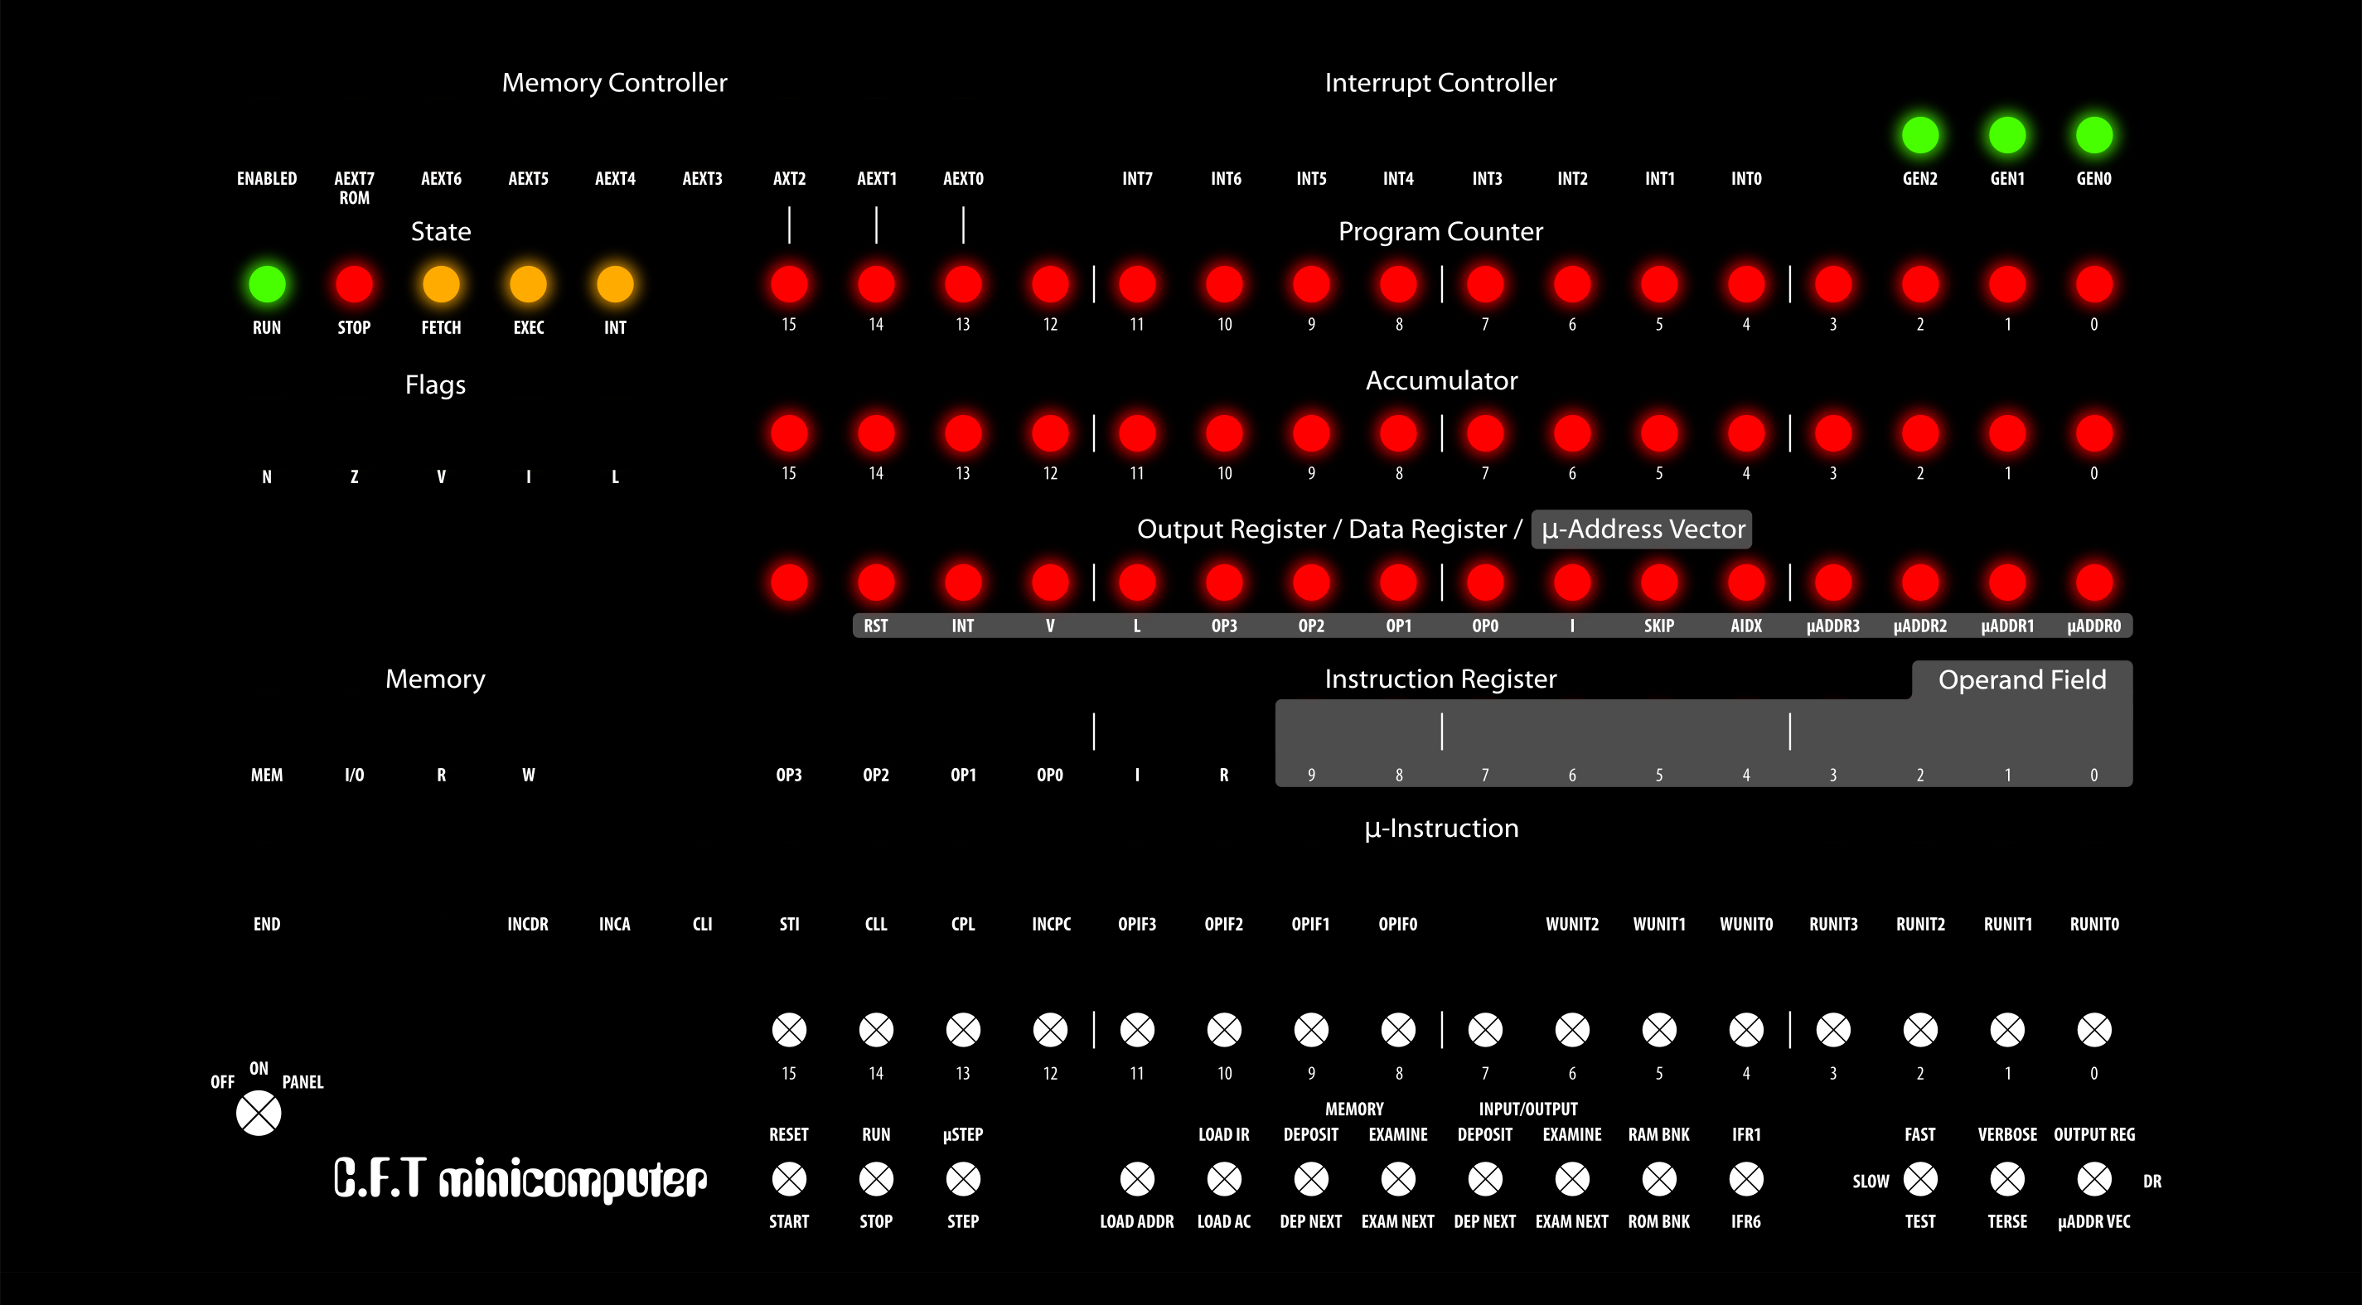
\includegraphics[width=\columnwidth]{figs/front-panel-v2-terse-small.jpg}\\
\caption{\label{fig-panel-terse}A mock-up of the front panel running in \sw{TERSE} mode.}
\end{figure}

\subsection{Power}

A key switch at the lower right controls power. At the leftmost position, the
computer is off. When the key is turned one position to the right, the computer
is activated with most panel switches locked. With the key int he rightmost
position, all panel switches are unlocked and the panel may be used in its
entirety.

\section{Using the Front Panel}

This section describes how to use the computer via the front panel.

\subsection{Power}

Insert the key in the key switch. Turn the key to the \sw{PANEL}
position. The computer activates, performs power supply diagnostics,
goes through a reset cycle, and halts itself. The \lt{STOP} light
should illuminate at this point, and the Program Counter will indicate
a binary address of {\sf 1111·1111·1111·0000}, or {\sf FFF0}.

\subsection{Boot from ROM}

With the computer freshly powered up and halted, or halted and reset,
move the \sw{ROM BNK}/\sw{RAM BNK} switch to the \sw{ROM BNK}
position.

Depress the \sw{RUN} or \sw{START} switch.

The computer boots from ROM and begins execution.

You may now secure the front panel by turning the key switch to the
\sw{ON} position.

\subsection{Toggle in Boot Code}

Ensure the computer is freshly powered up and halted, or halted and reset.

Set the Switch Register for a low value such as {\sf
  0000·0100·0000·0000} (1kWord from start of memory). Depress \sw{SET
  ADDR}.

Set the Switch Register for the first value of the bootstrap
code. Depress \sw{MEMORY DEP NEXT}. Repeat as required.

Reset the Switch Register for the initial address of the bootstrap
program. Depress \sw{SET ADDR}.

Depress \sw{RUN}. The computer starts execution of the code from the
specified address.

You may now secure the front panel by turning the key switch to the
\sw{ON} position.

\subsection{Halting the Computer Forcibly}

With the key switch in the \sw{PANEL} position, depress \sw{STOP}. The
computer halts.

\subsection{Resetting the Computer}

With the key switch in the \sw{PANEL} position, depress \sw{RESET} or
\sw{START}. The computer resets. If the computer is running, ROM must
be fitted and the \sw{ROM BNK}/\sw{RAM BNK} switch must be in the
\sw{ROM BNK} position.

\subsection{Debugging with the Front Panel}

The front panel may be used to interrupt normal computer operation and
inspect or modify its state for debugging purposes. The computer can
then resume operation. The user should, however, be aware of a number
of considerations when using the front panel to do this:

\begin{itemize}
\item Operating the \sw{STOP} switch halts the computer
  mid-instruction. With a microprogram in execution, registers and
  control units may change. If necessary, the \sw{uSTEP} switch should
  be operated to complete the microprogram, that is until the
  \lt{FETCH} light illuminates. After which, if desired, the
  \sw{uSTEP} switch may be operated repeatedly until the \lt{EXECUTE}
  light illuminates, at which point an instruction has just been
  fetched and is about to be executed. It is safe to use the front
  panel for macro-debugging at this point.
\item Using the \sw{SET ADDR} switch modifies the \PC. When the
  computer resumes operation, this will effectively jump to the
  address set via the front panel. If this is not desired, the user
  must note the value of the \PC and manually restore it before
  continuing.
\item Using the memory and I/O functions also cause the \MAR{} to
  change. This is safe to do when using the {\sf STEP} switch, but not
  mid-microprogram.
\item Obviously, modifying the \IR{}, memory or I/O devices can have
  side effects on the running of the computer, but this is a desired
  feature of any control panel.
\end{itemize}

\section{Hardware Guide}

The Front Panel comprises three distinct parts (though parts 2 and 3
may be implemented on the same physical board):

\begin{enumerate}
\item{\bf The Front Panel Controller Card} contains most of the front
  panel logic.
\item{\bf The Front Panel Driver and LED Board} hosts the LEDs and
  their drivers, as well as the Multi-Function display logic. The LED
  banks are connected directly to the corresponding processor hardware
  (e.g. the register card) using 8 or 9-conductor flat cables.
\item{\bf The Front Panel Debounce and Switch Board} hosts the switches
  and their debounce circuitry.
\end{enumerate}

The controller connects to the switch and LED boards via a
daisy-chained 40-conductor ribbon cable.

\begin{table*}[h!]
  \caption{\label{tab-connectors}Connections between the front panel
    and the processor.}
  \centering
  \begin{tabular}{llcll}
    \noalign{\smallskip}\hline\noalign{\smallskip}
    Function & Name & Conductors & From & To \\
    \noalign{\smallskip}\hline\noalign{\smallskip}
    Switch Register Low      & CON1  & 8 & Switch board & Front Panel Controller \\
    Switch Register High     & CON2  & 8 & Switch board & Front Panel Controller \\
    Memory Banking Status    & CON3  & 9 & Memory Banking board & Front Panel LED board \\
    \A{} Low                 & CON4  & 8 & Register or ALU board & Front Panel LED board \\
    \A{} High                & CON5  & 8 & Register or ALU board & Front Panel LED board \\
    \PC{} Low                & CON6  & 8 & Register board & Front Panel LED board \\
    \PC{} High               & CON7  & 8 & Register board & Front Panel LED board \\
    \IR{} Low                & CON8  & 8 & Control board & Front Panel LED board \\
    \IR{} High               & CON9  & 8 & Control board & Front Panel LED board \\
    Microcode Vector Low     & CON10 & 8 & Control board & Front Panel LED board \\
    Microcode Vector Medium  & CON11 & 8 & Control board & Front Panel LED board \\
    Microcode Vector High    & CON12 & 8 & Control board & Front Panel LED board \\
    Flags                    & CON13 & 5 & Control board \& ALU & Front Panel LED board \\
    Output Register Low      & CON14 & 8 & Front Panel Controller & Front Panel LED board \\
    Output Register High     & CON15 & 8 & Front Panel Controller & Front Panel LED board \\
    \DR{} Low                & CON16 & 8 & Register board & Front Panel LED board \\
    \DR{} High               & CON17 & 8 & Register board & Front Panel LED board \\
    Microcode Address Low    & CON18 & 8 & Control board & Front Panel LED board \\
    Microcode Address High   & CON19 & 7 & Control board & Front Panel LED board \\
    Interrupt Flag Status    & CON20 & 8 & Interrupt Controller board & Front Panel LED board \\
    Interrupt Enable Status  & CON21 & 8 & Interrupt Controller board & Front Panel LED board \\
    Control switches 1       & CON22 & 8 & Switch board & Front Panel Controller \\
    Control switches 2       & CON23 & 8 & Switch board & Front Panel Controller \\
    Clock Control            & CON24 & 3 & Switch board & Clock Generator \\
    Memory Banking Control   & CON25 & 2 & Switch board & Memory Banking board \\
    Interrupt Control        & CON26 & 3 & Switch board & Interrupt Controller board \\
    Reset In                 & CON27 & 1 & Switch board & Reset generator \\
    Miscellaneous LEDs (×3)  & SV1   & 6 & Any required & Front Panel LED board \\
    \noalign{\smallskip}\hline\noalign{\smallskip}
  \end{tabular}
\end{table*}


\subsection{Connections}

The front panel boards connect to the processor by means of numerous
8-way connectors, shown in~\tcf{tab-connectors}.

\section{Further reading}

For further information on the CFT computer, please consult the
following URL:

\begin{center}
\link{www.bedroomlan.org/hardware/cft}
\end{center}

\clearpage

\begin{figure*}
\centering
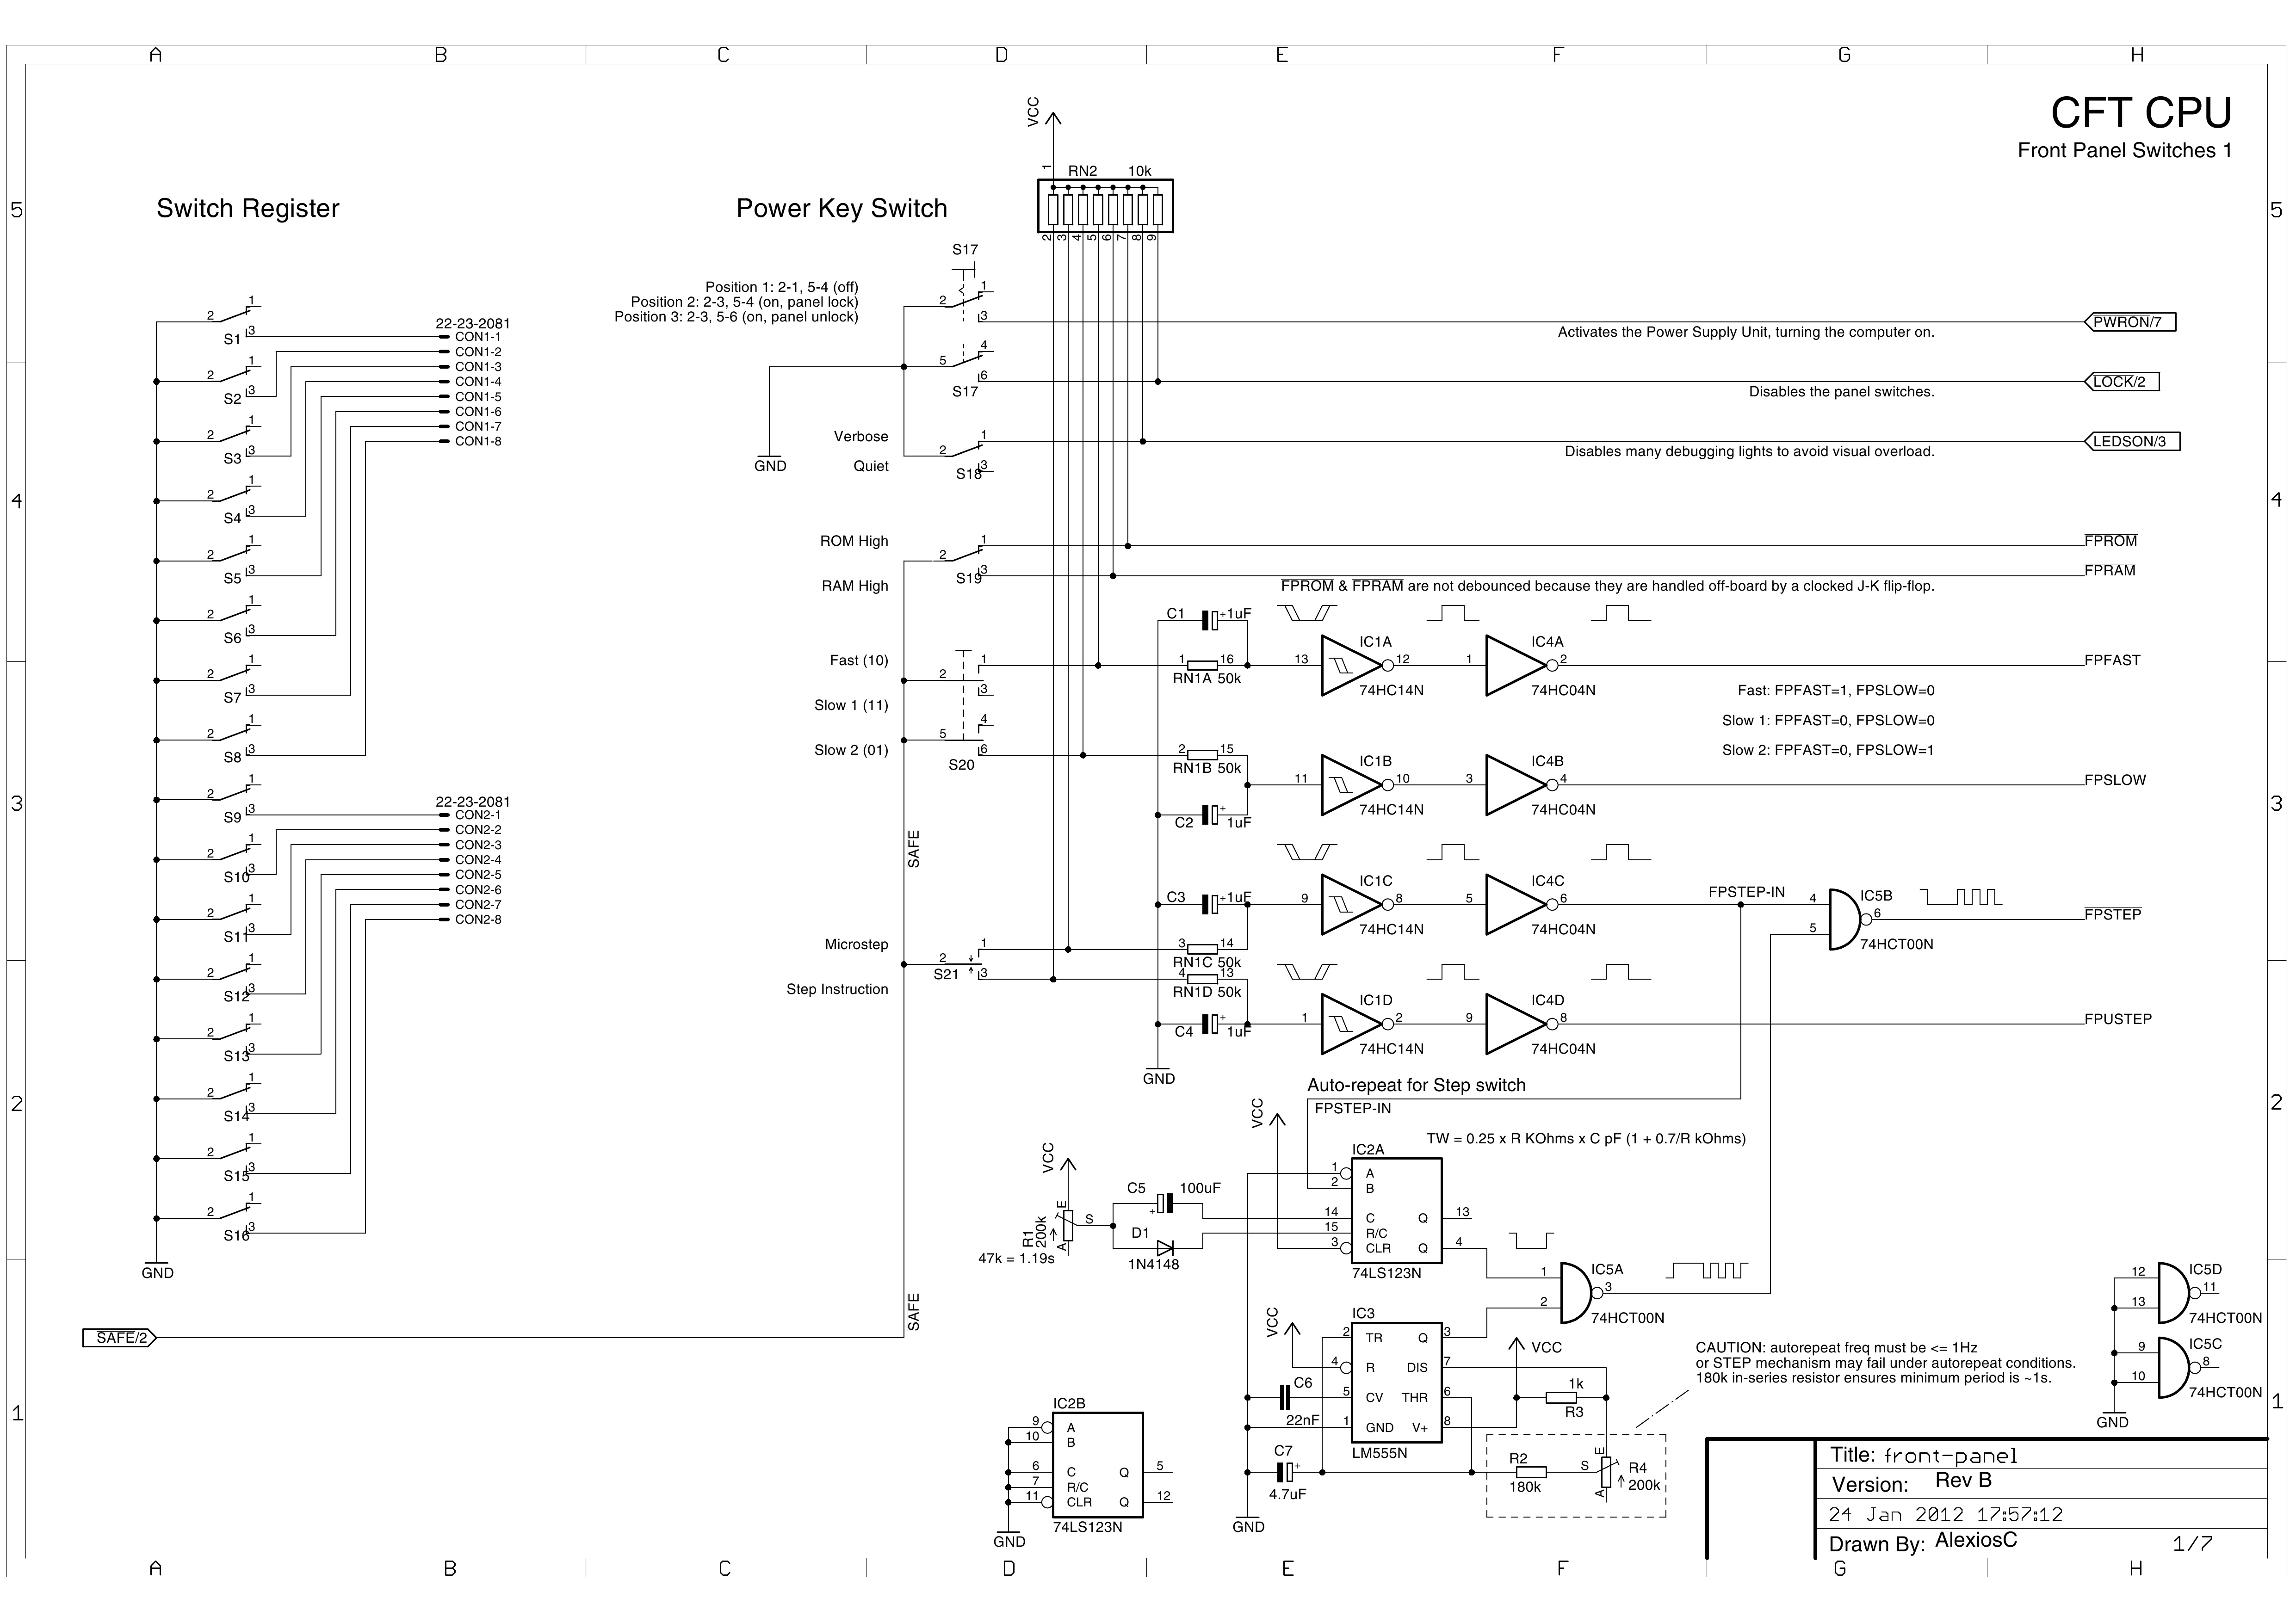
\includegraphics[width=0.95\textheight,angle=90]{figs/front-panel-1.jpg}\\
\caption{\label{fig-schematic-front-panel-1}Schematic drawing of the front panel LED and switch boards (1 of 7).}
\end{figure*}

\begin{figure*}
\centering
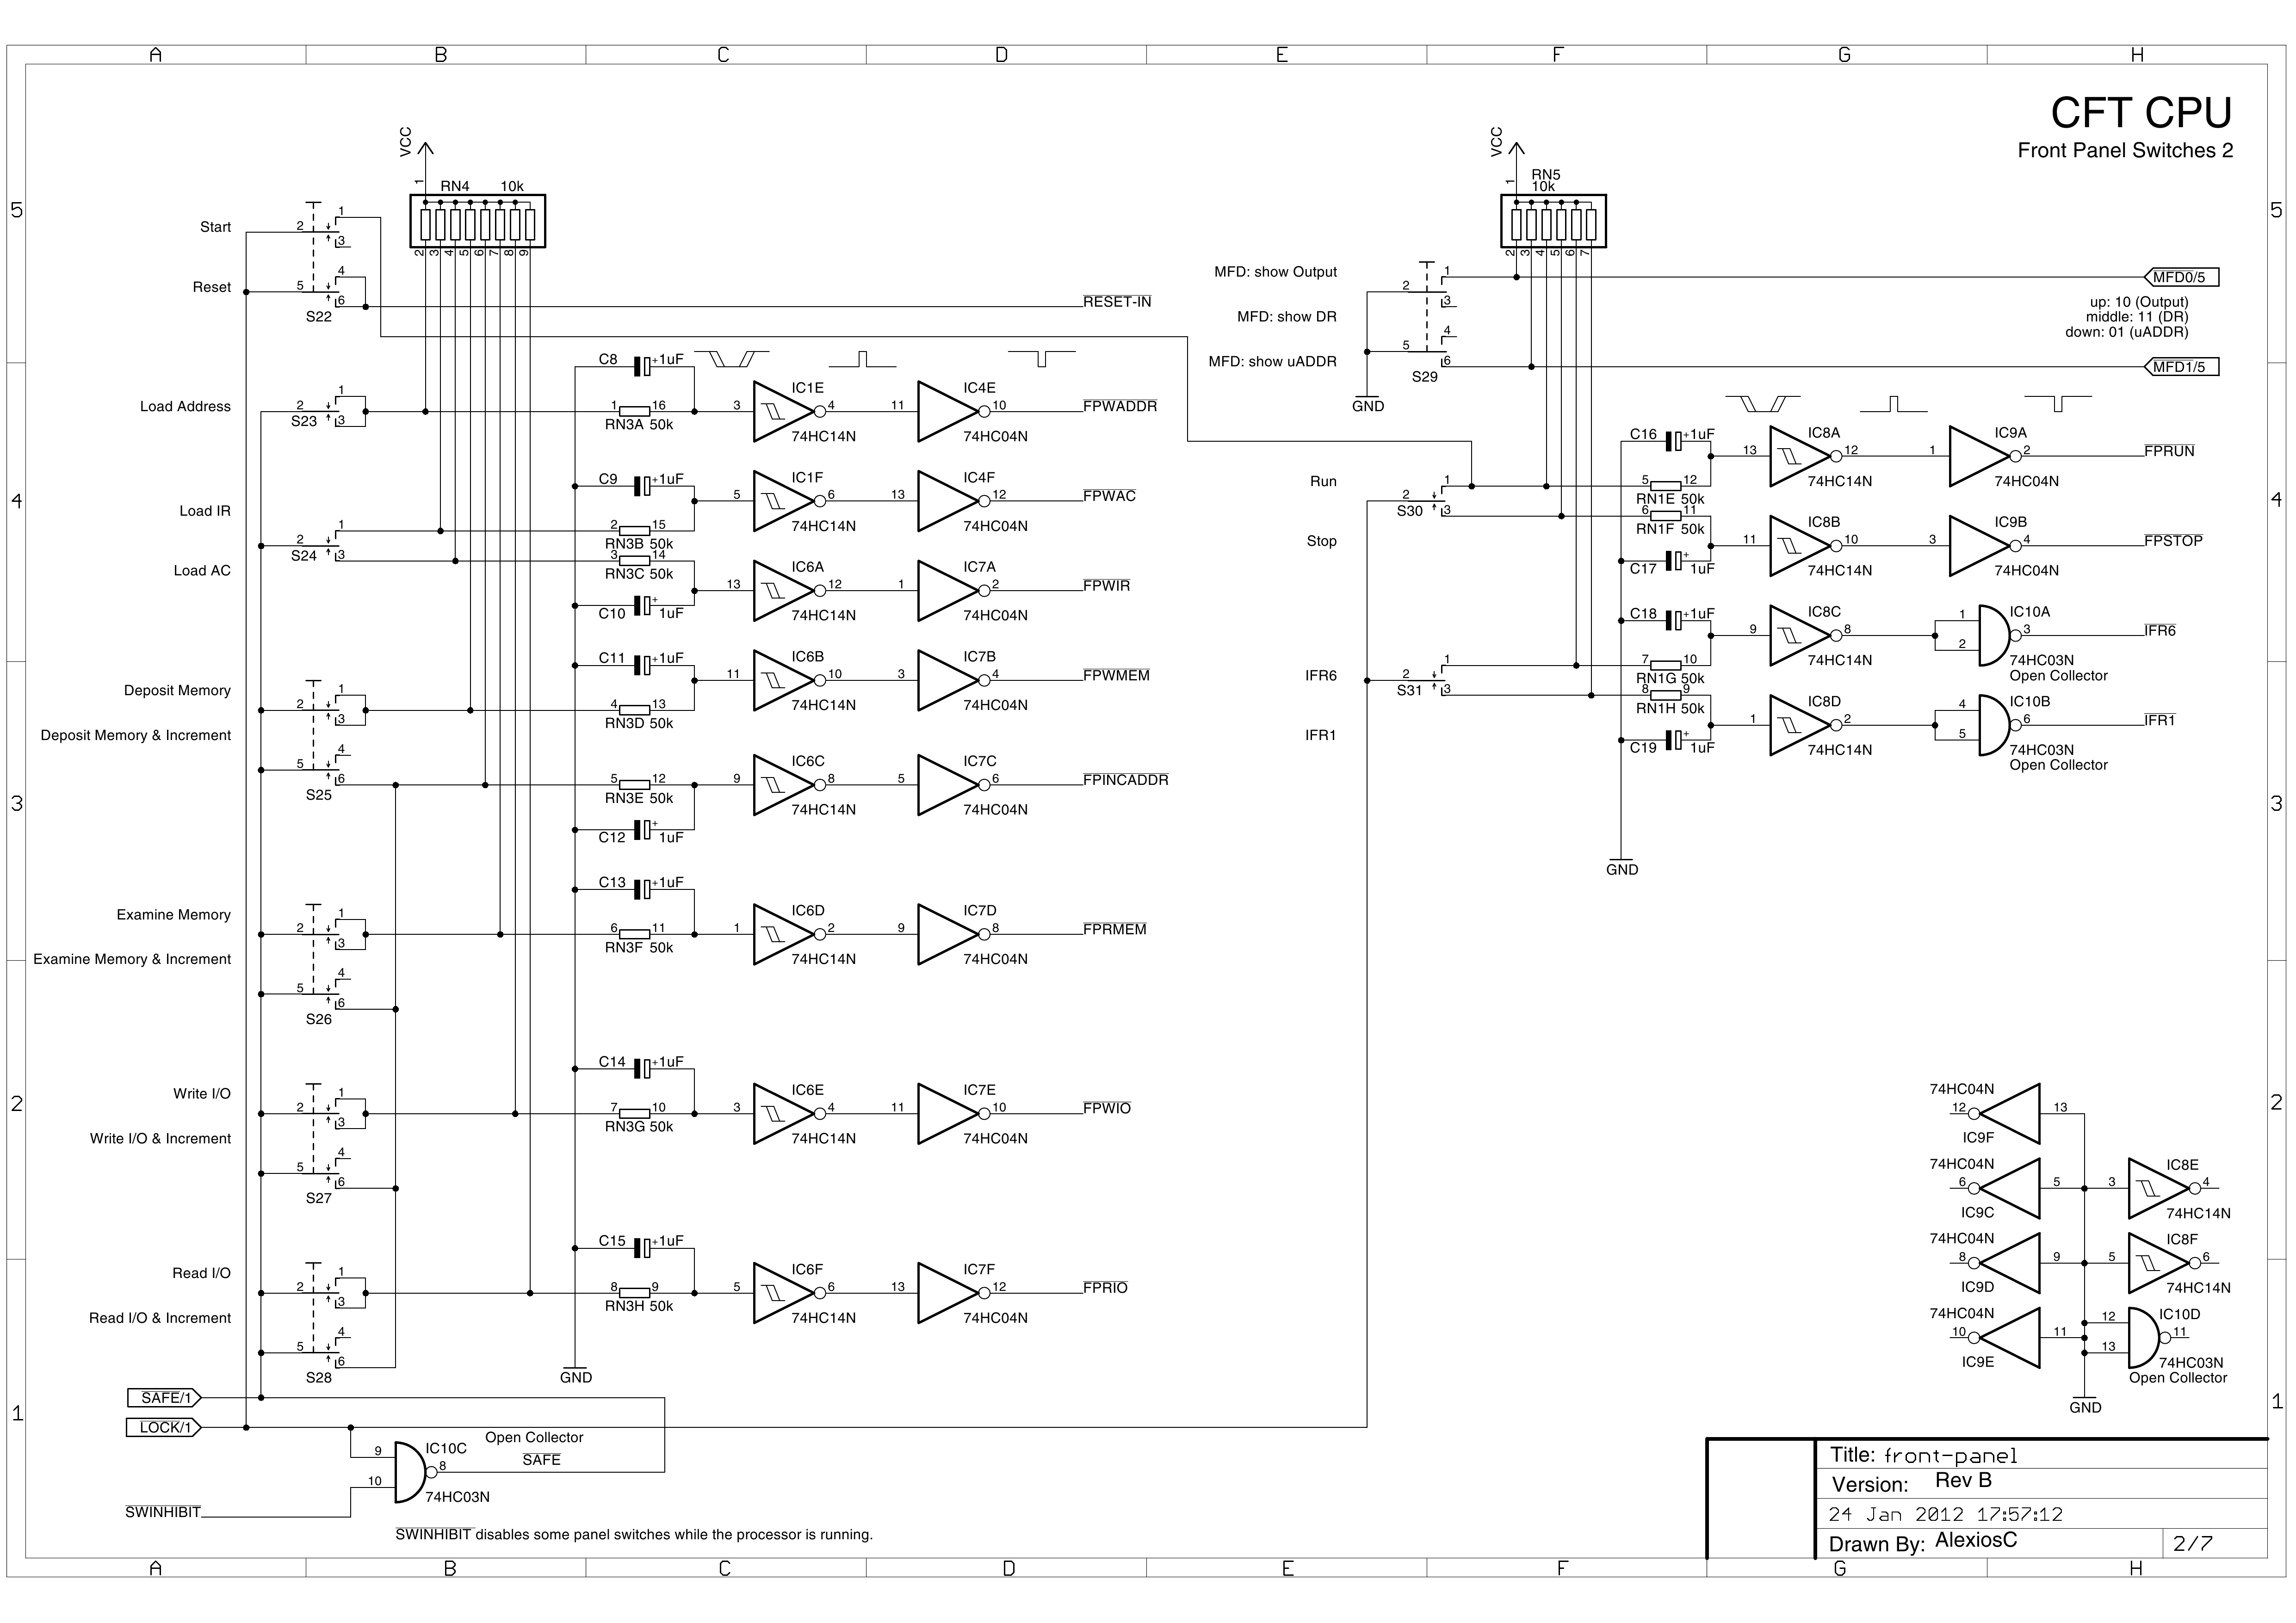
\includegraphics[width=0.95\textheight,angle=90]{figs/front-panel-2.jpg}\\
\caption{\label{fig-schematic-front-panel-2}Schematic drawing of the front panel LED and switch boards (2 of 7).}
\end{figure*}

\begin{figure*}
\centering
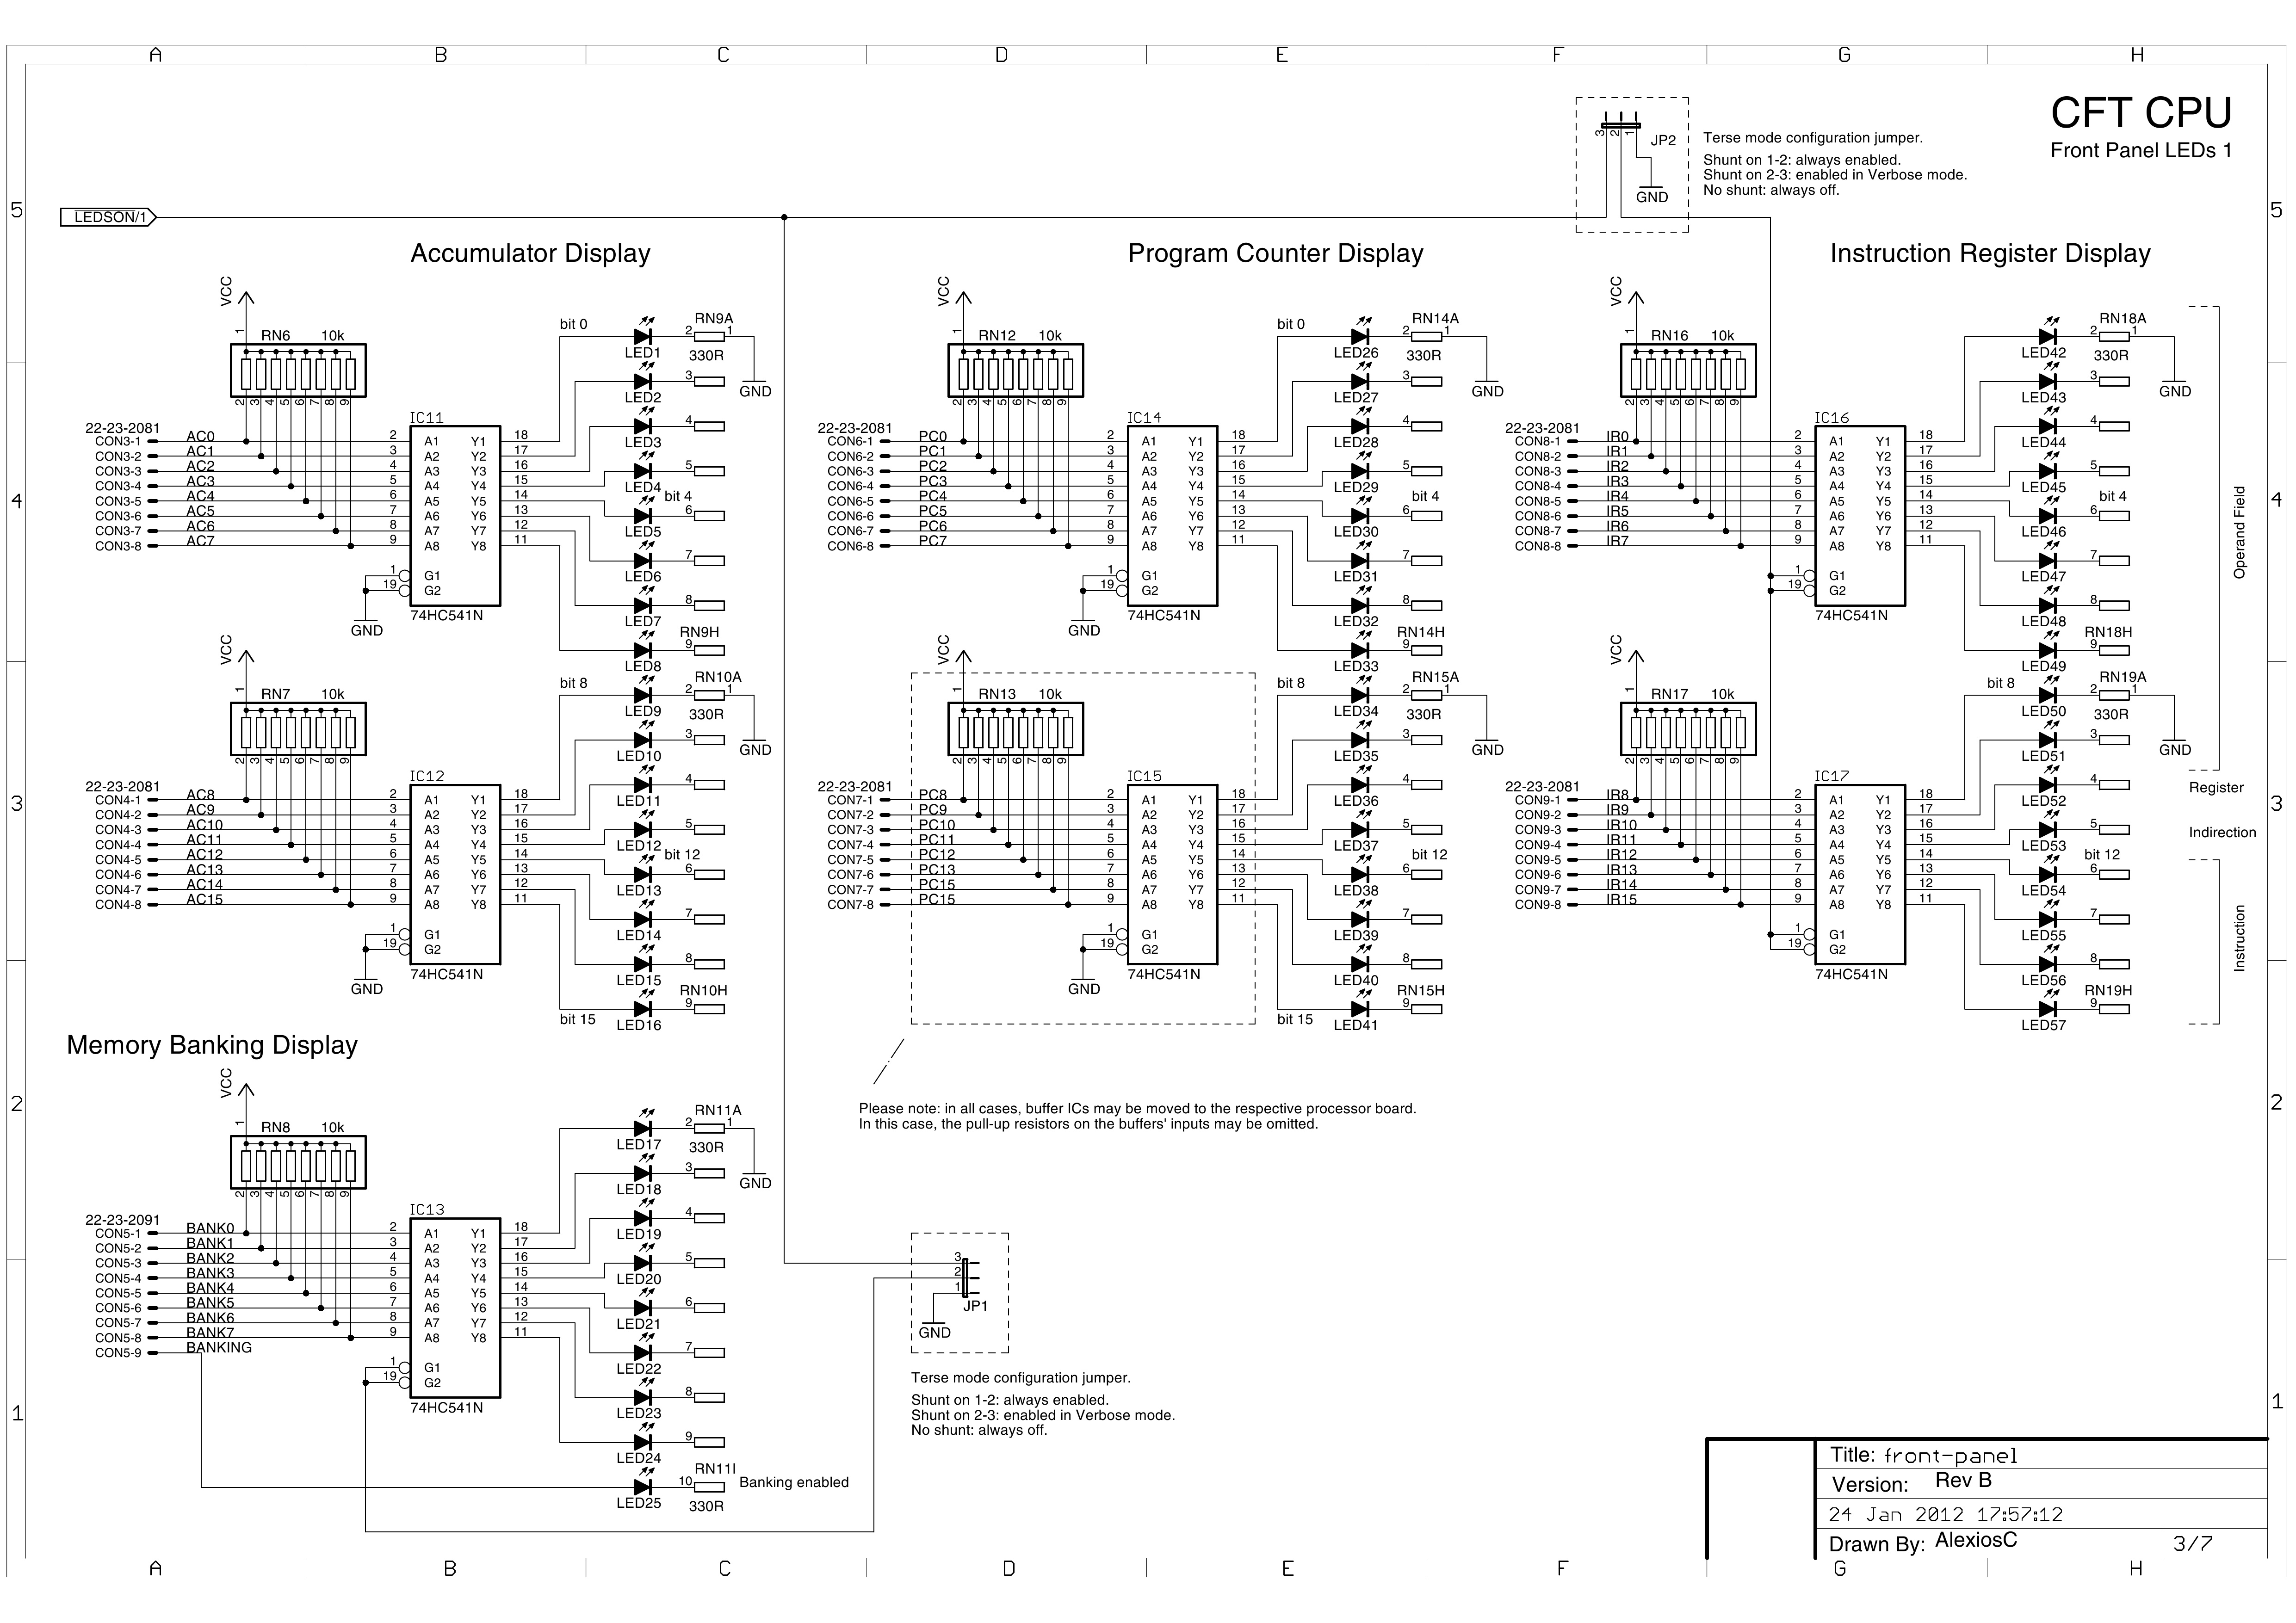
\includegraphics[width=0.95\textheight,angle=90]{figs/front-panel-3.jpg}\\
\caption{\label{fig-schematic-front-panel-3}Schematic drawing of the front panel LED and switch boards (3 of 7).}
\end{figure*}

\begin{figure*}
\centering
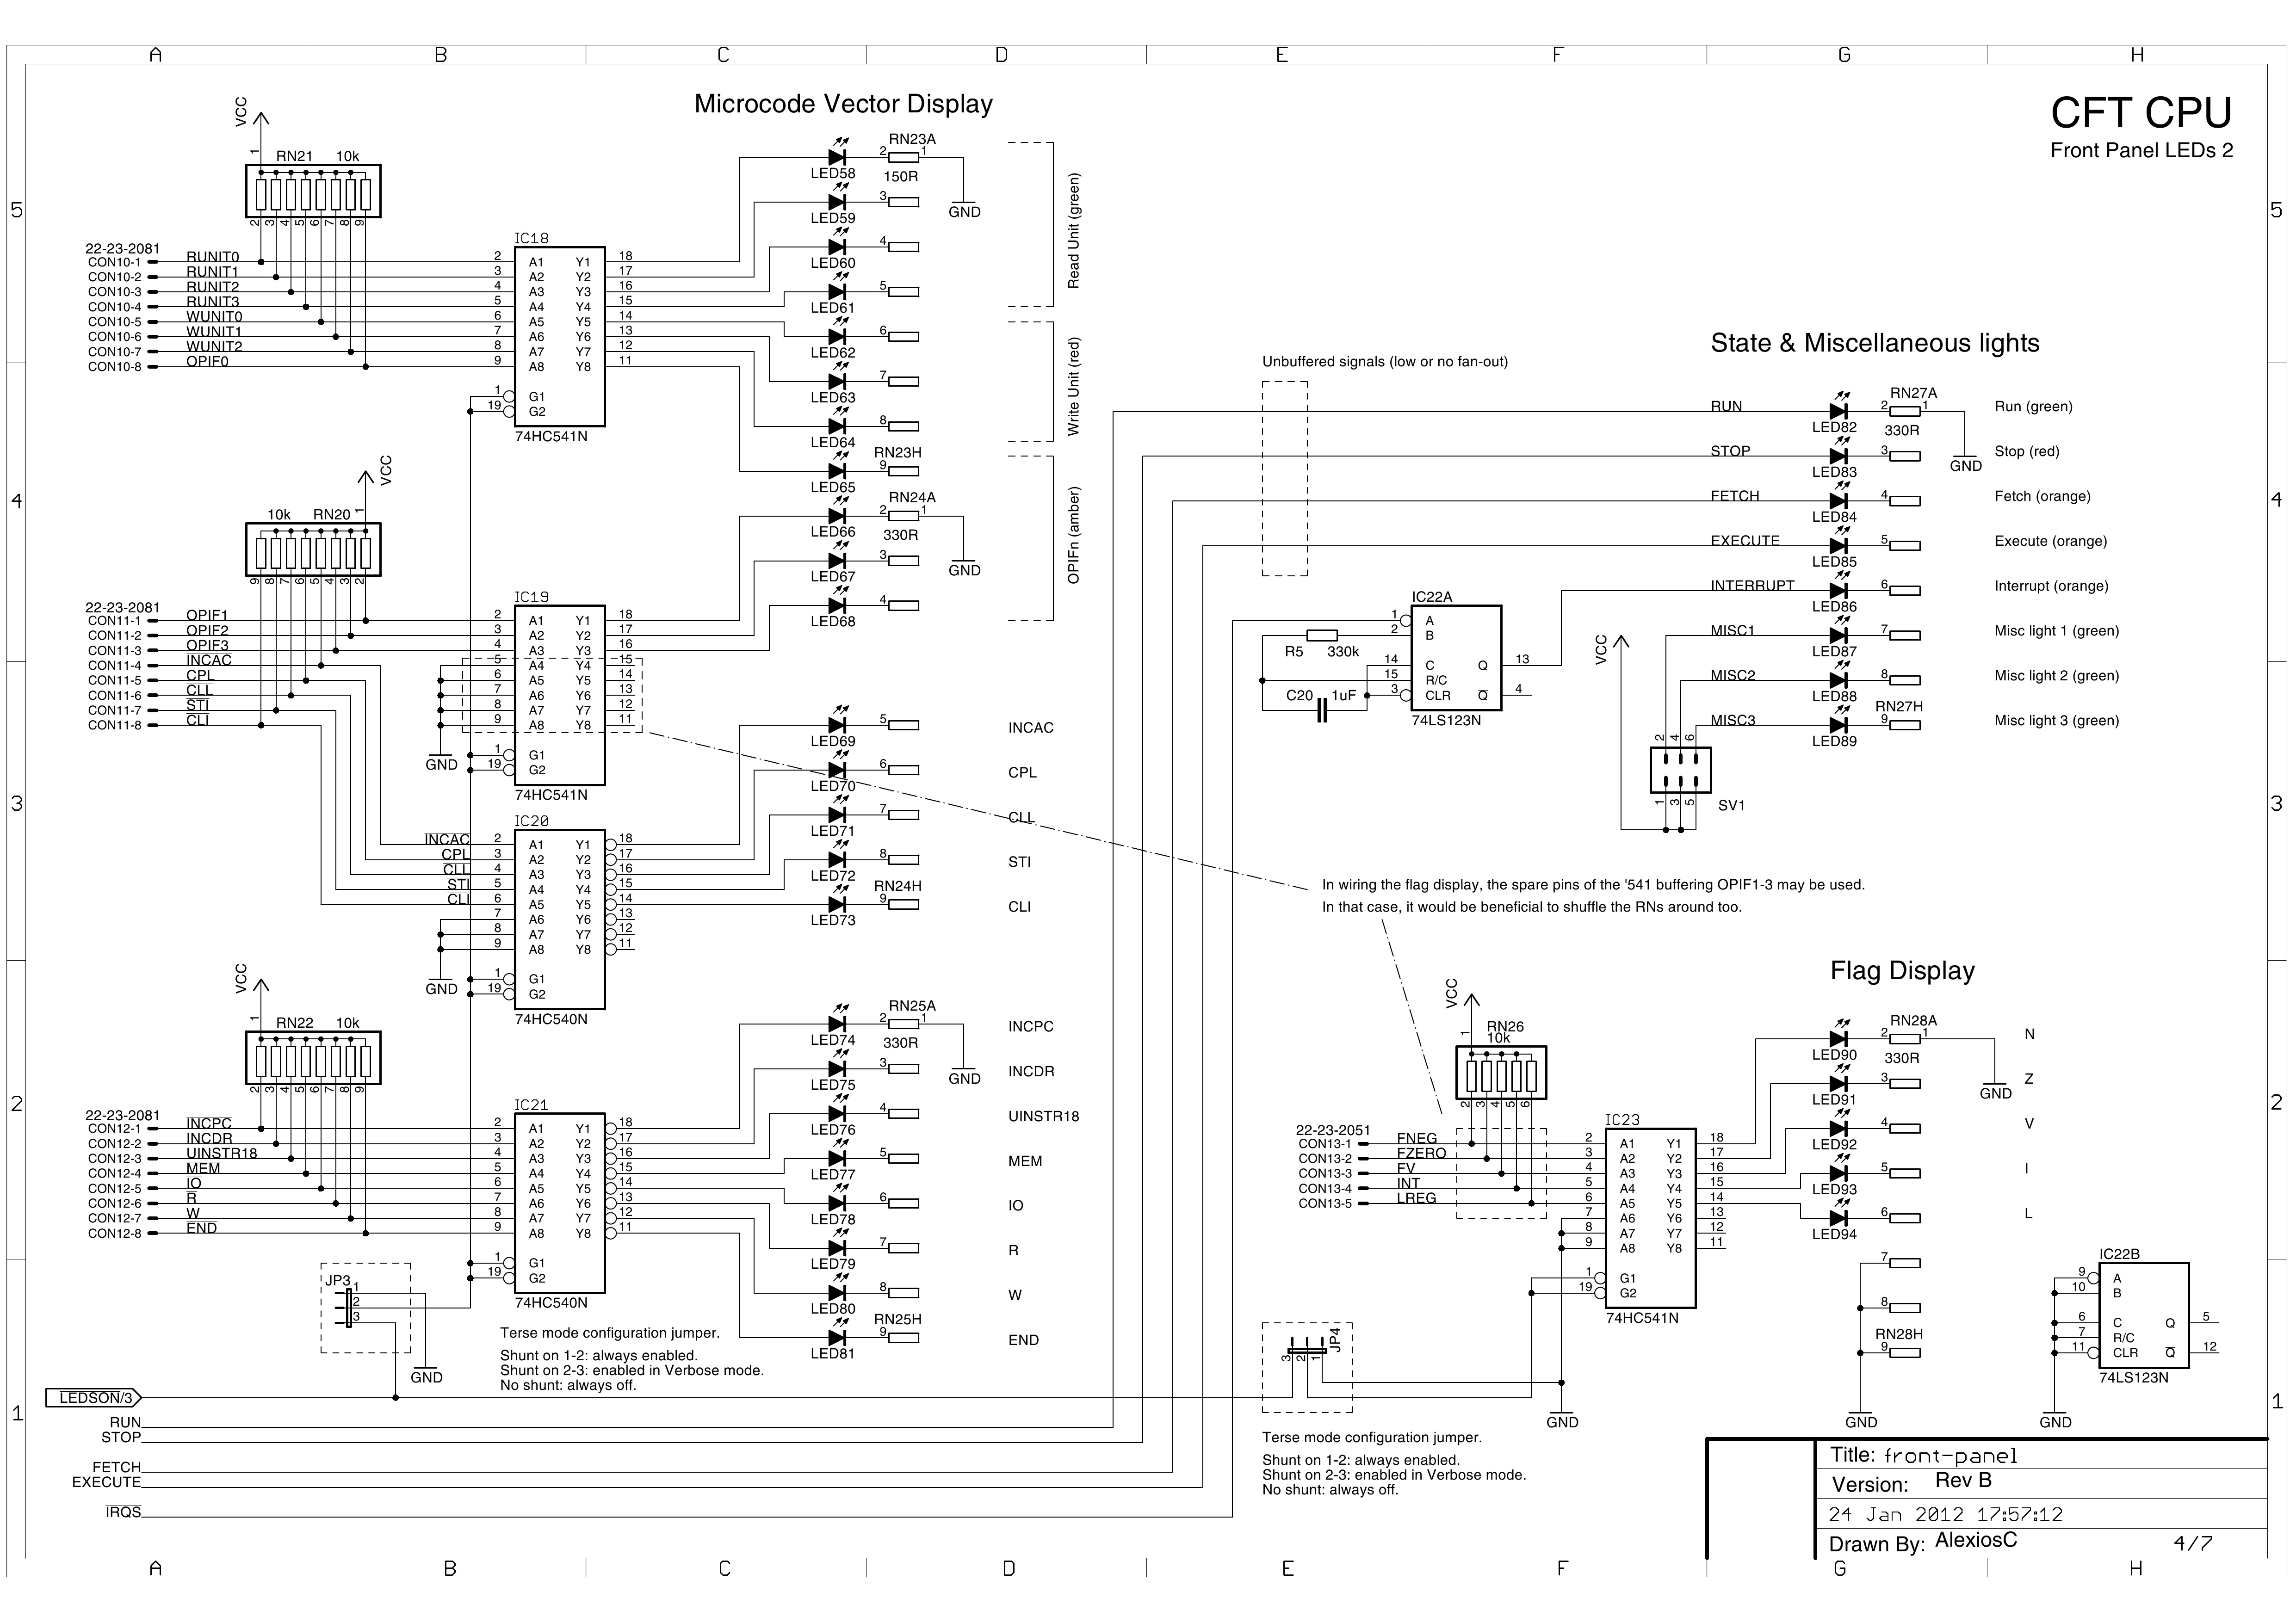
\includegraphics[width=0.95\textheight,angle=90]{figs/front-panel-4.jpg}\\
\caption{\label{fig-schematic-front-panel-4}Schematic drawing of the front panel LED and switch boards (4 of 7).}
\end{figure*}

\begin{figure*}
\centering
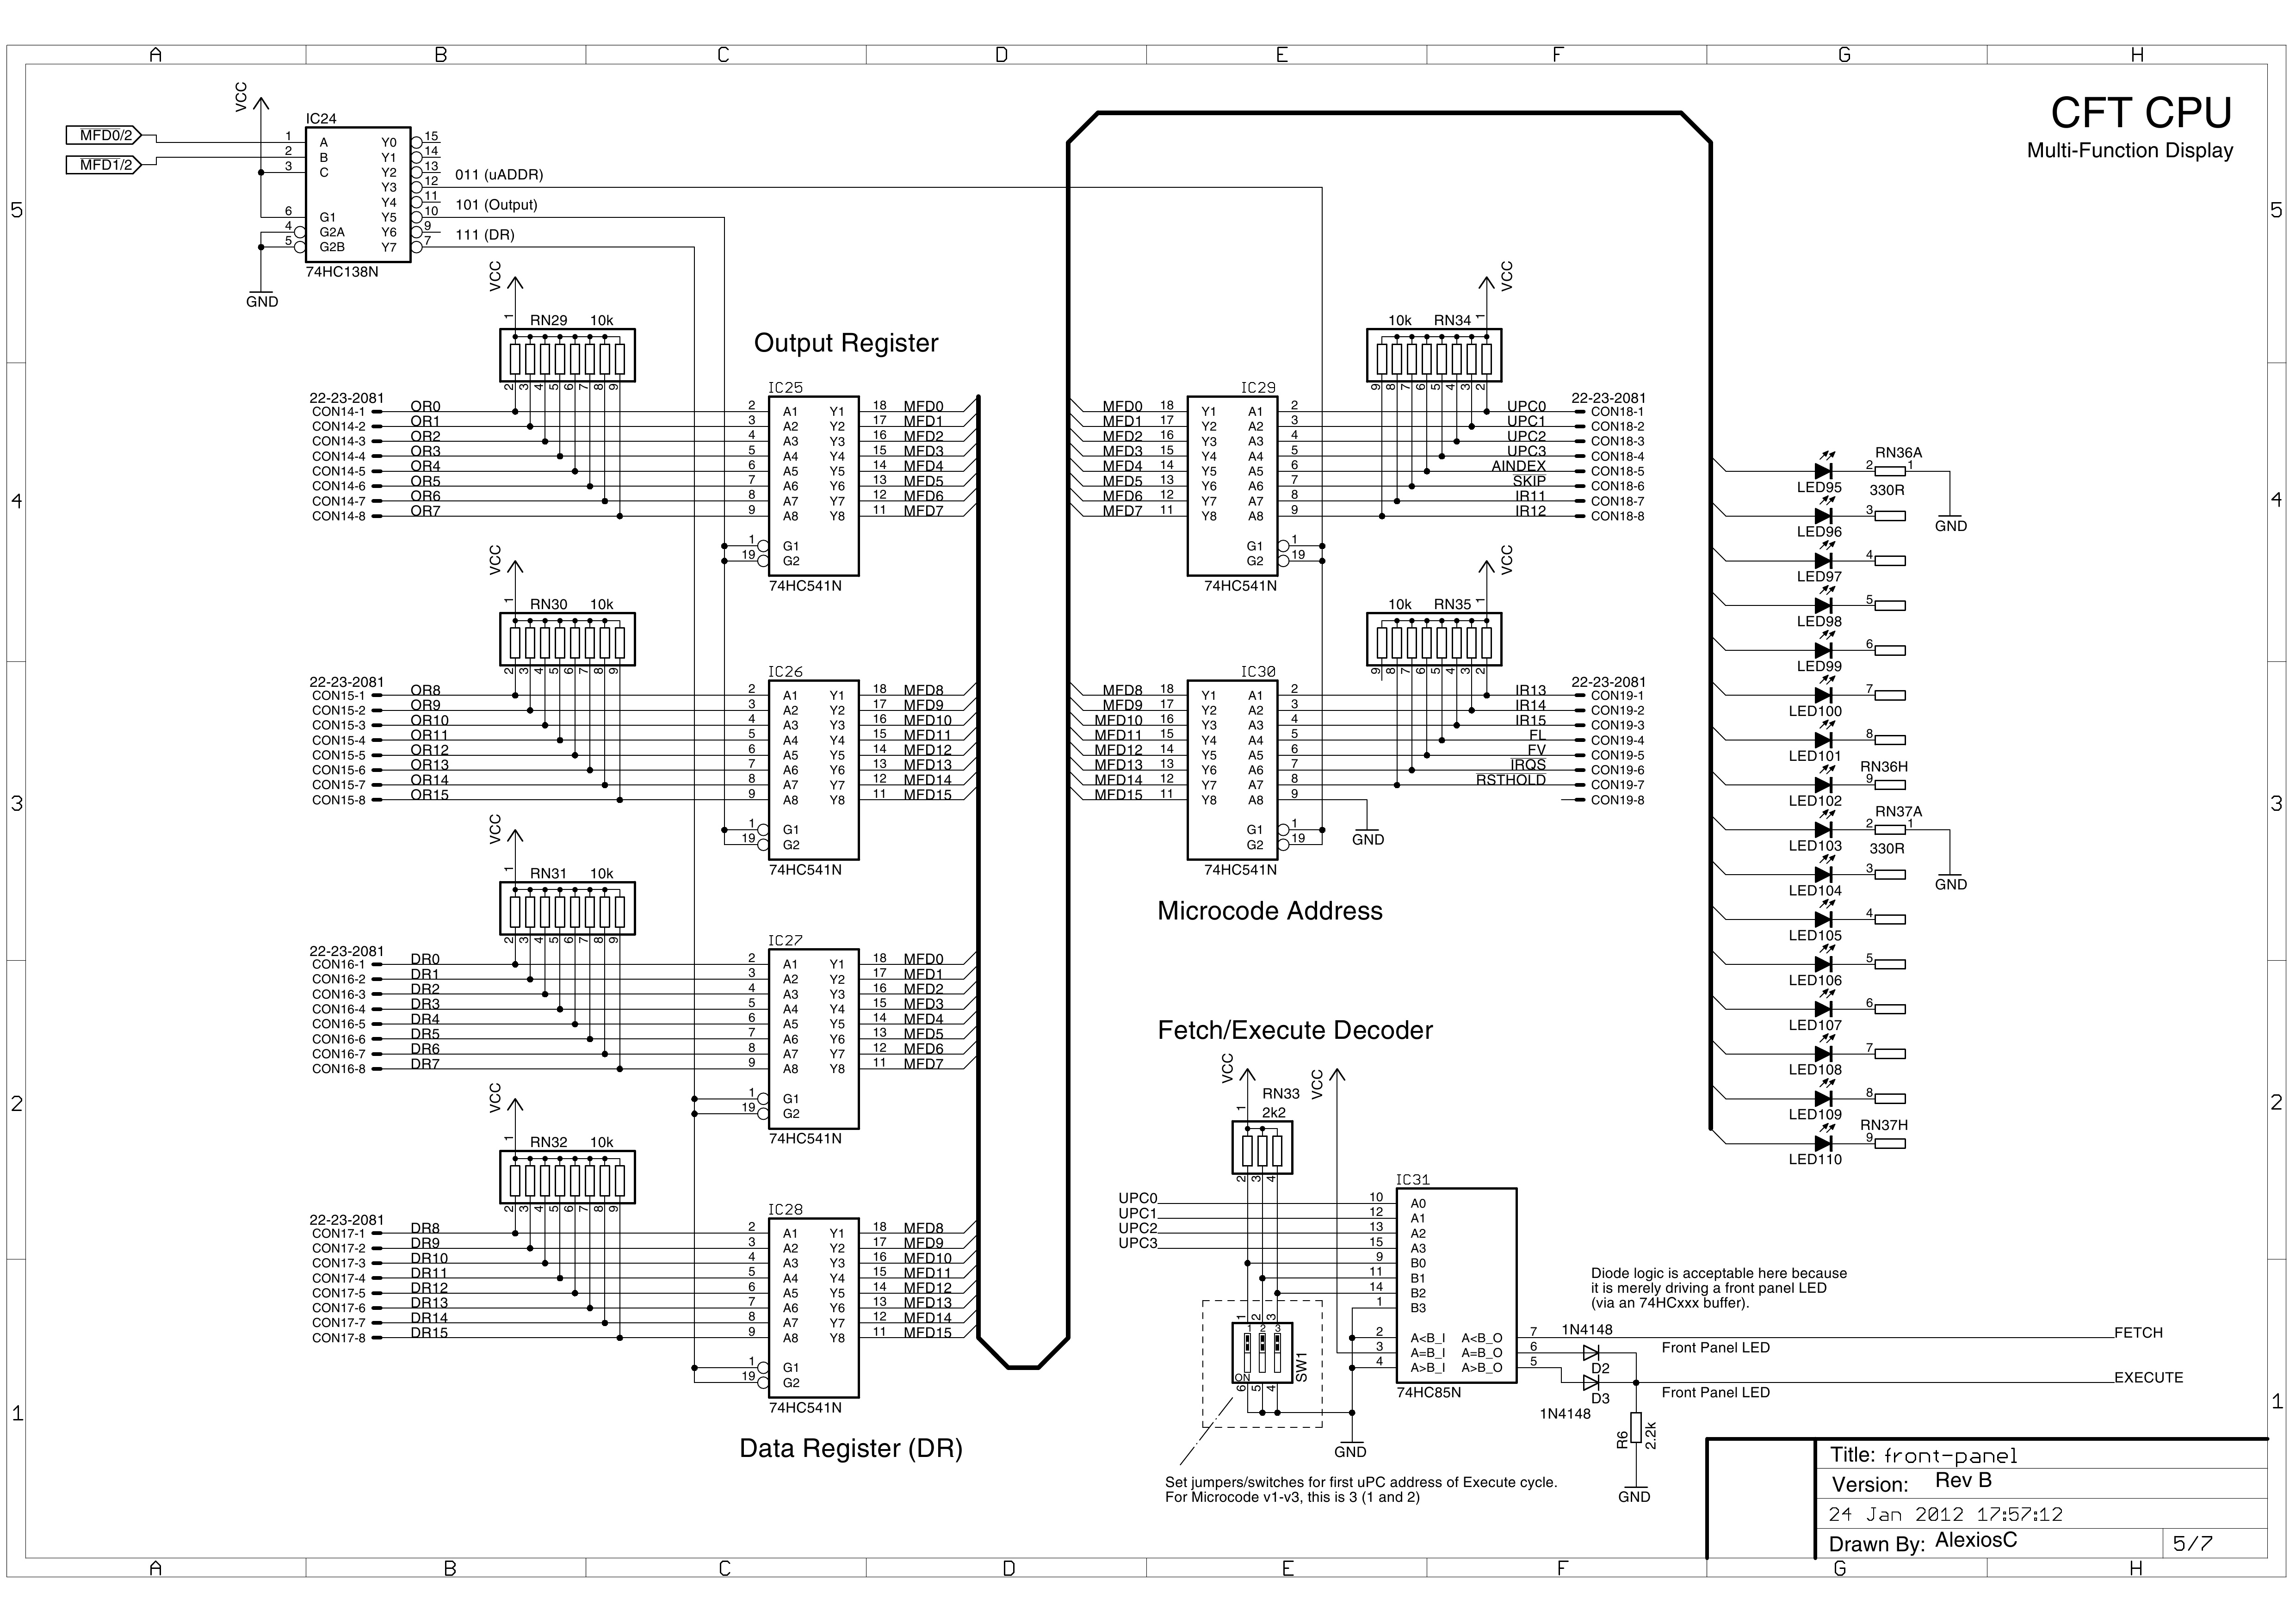
\includegraphics[width=0.95\textheight,angle=90]{figs/front-panel-5.jpg}\\
\caption{\label{fig-schematic-front-panel-5}Schematic drawing of the front panel LED and switch boards (5 of 7).}
\end{figure*}

\begin{figure*}
\centering
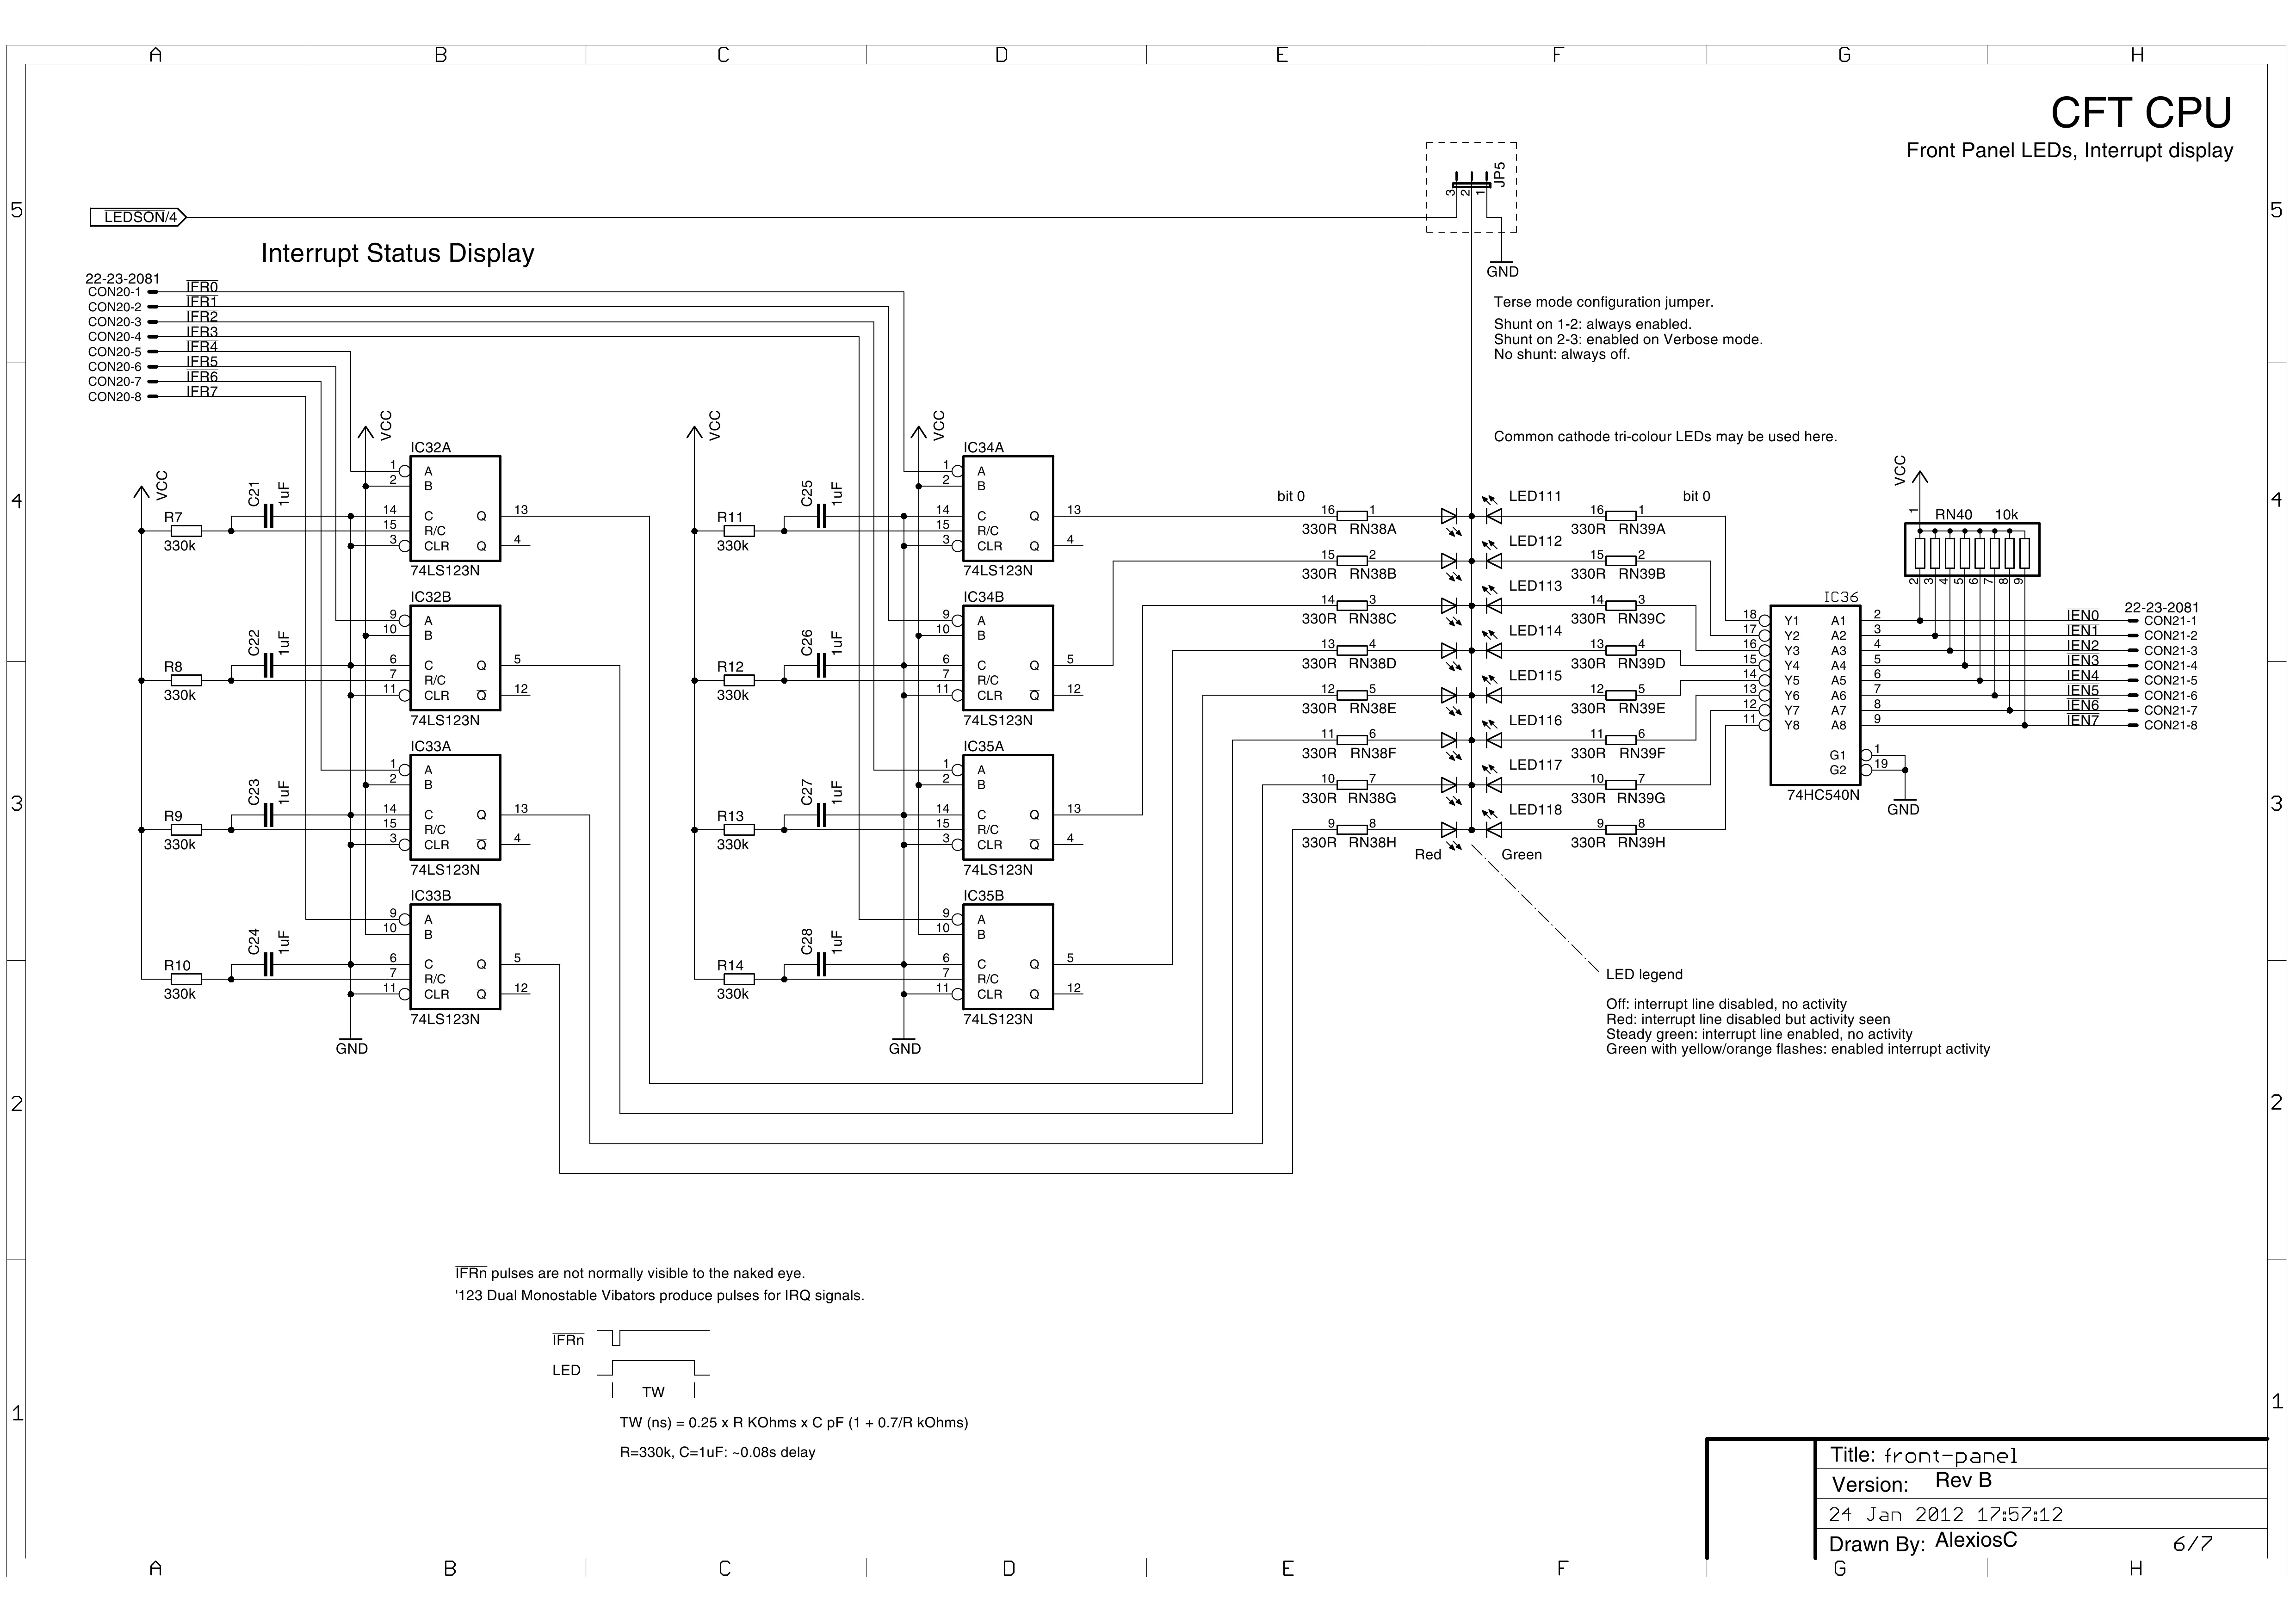
\includegraphics[width=0.95\textheight,angle=90]{figs/front-panel-6.jpg}\\
\caption{\label{fig-schematic-front-panel-6}Schematic drawing of the front panel LED and switch boards (6 of 7).}
\end{figure*}

\begin{figure*}
\centering
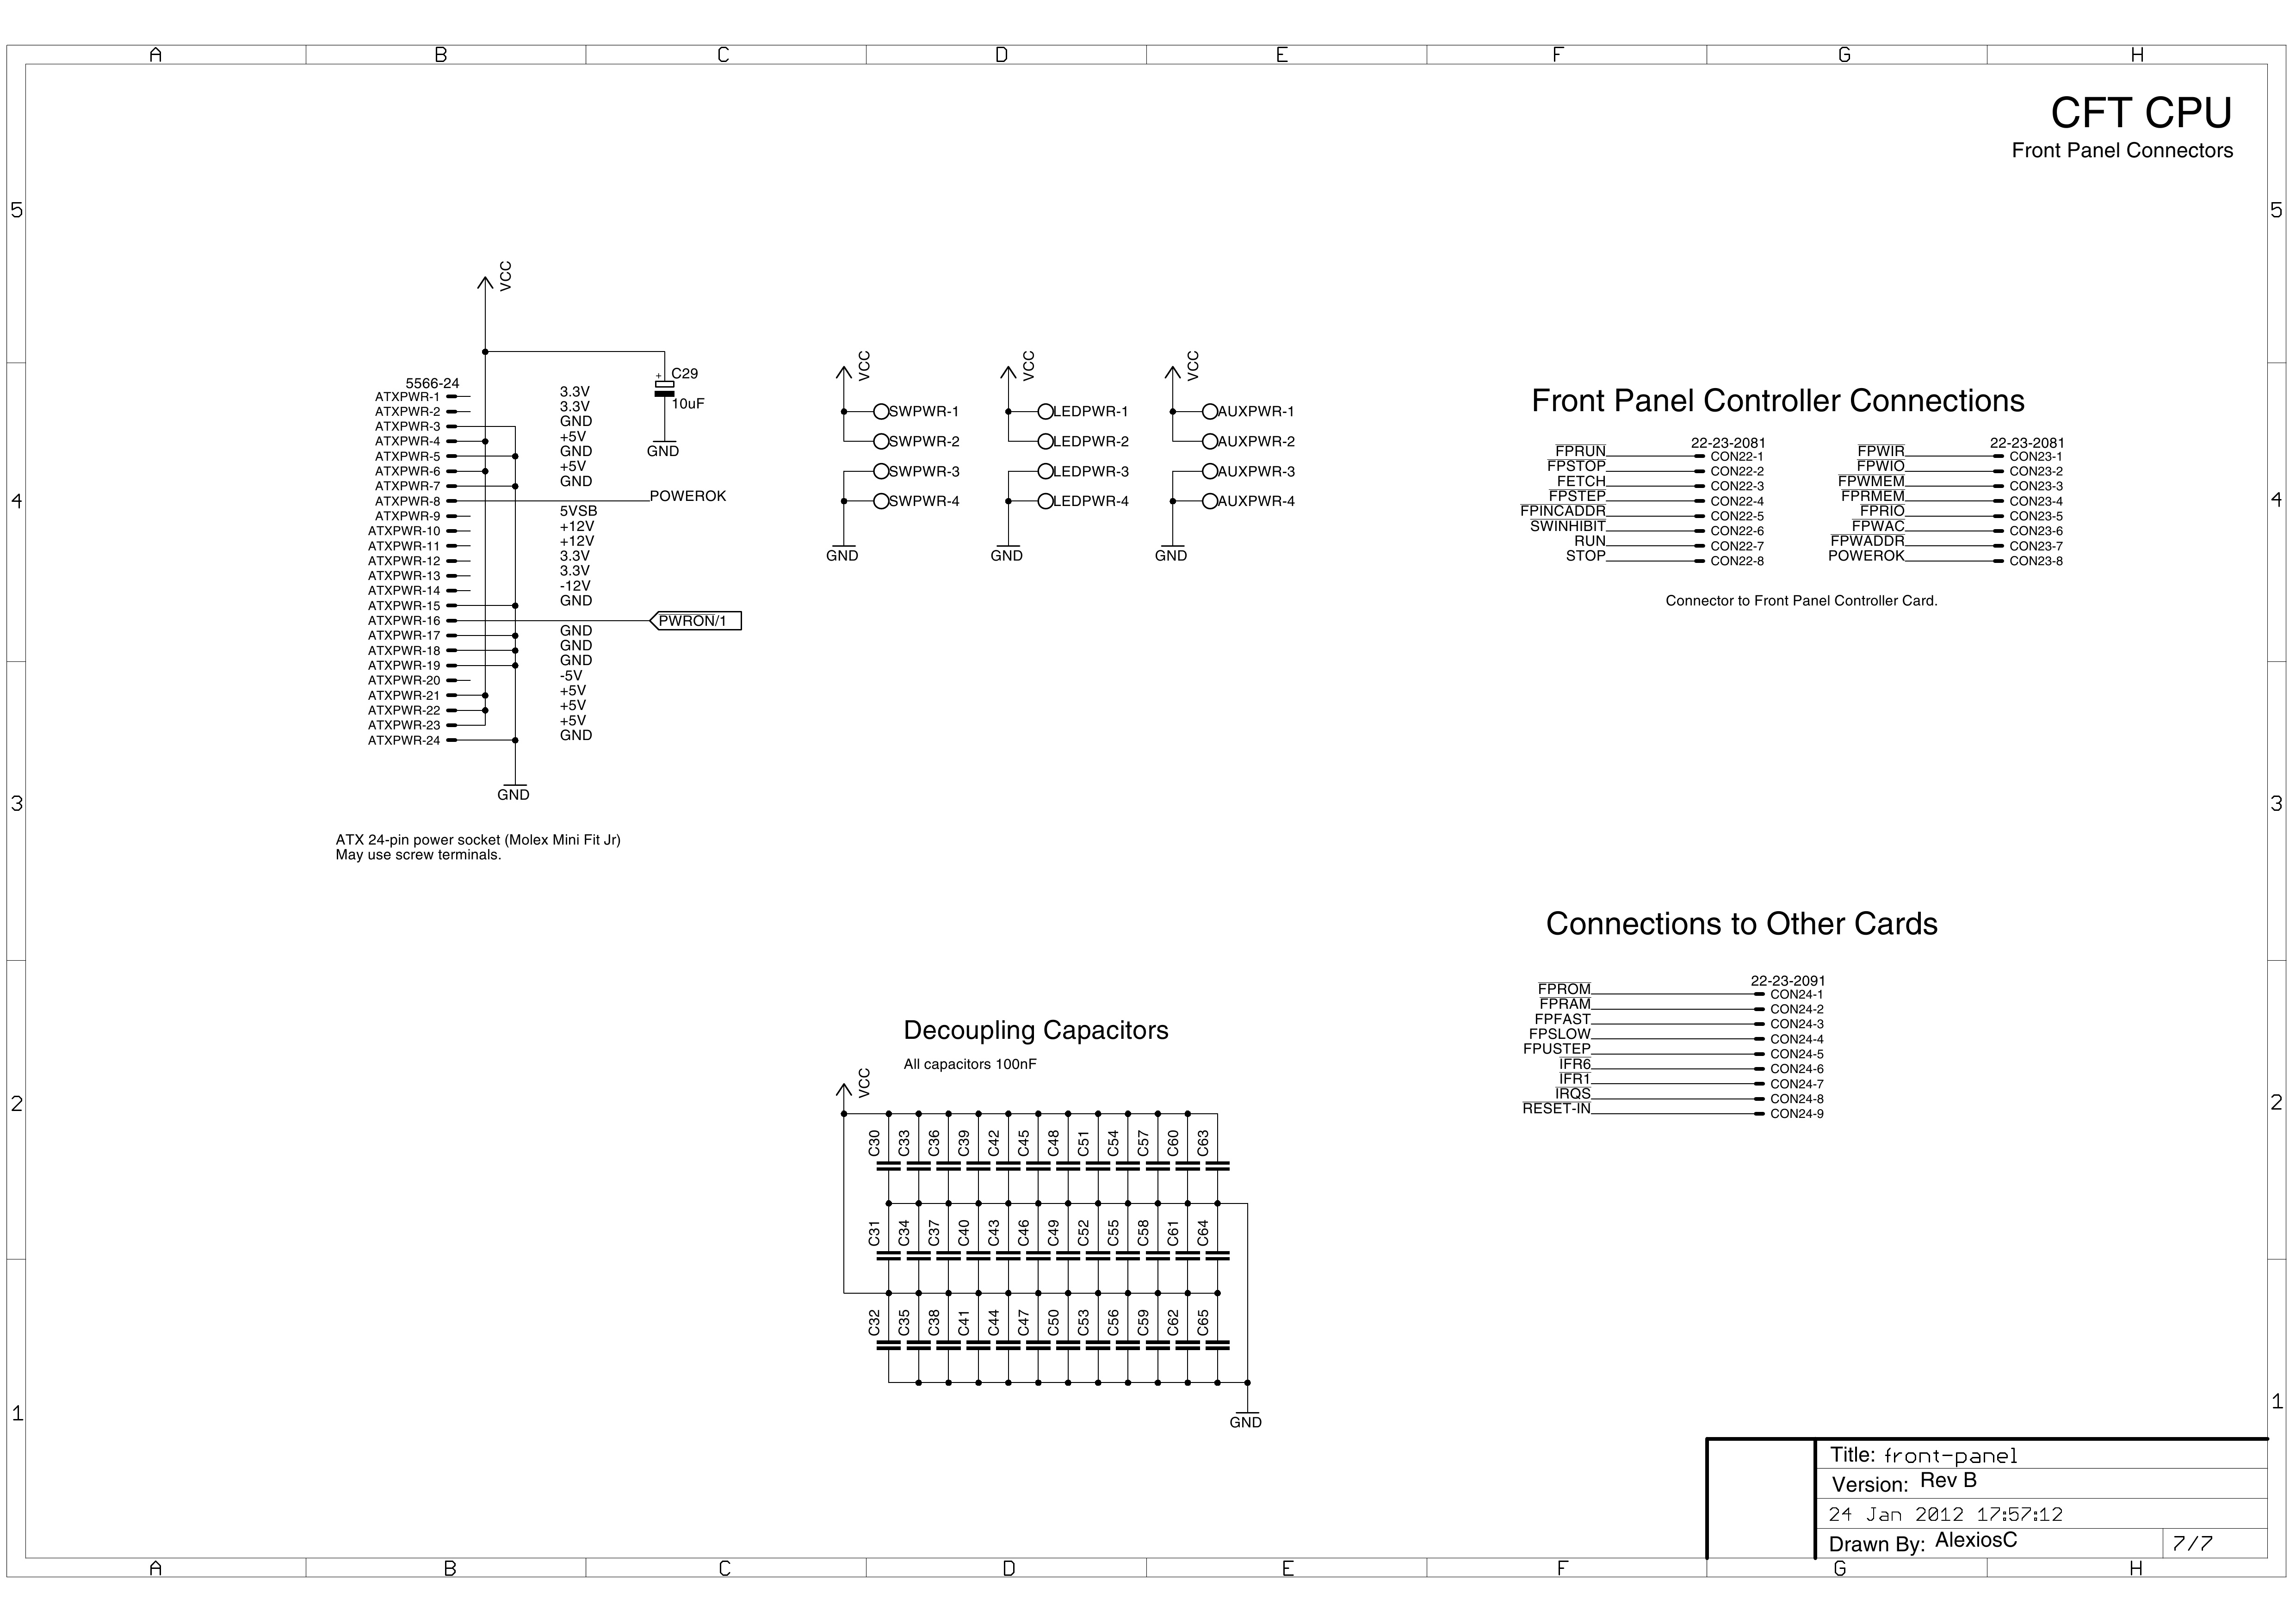
\includegraphics[width=0.95\textheight,angle=90]{figs/front-panel-7.jpg}\\
\caption{\label{fig-schematic-front-panel-7}Schematic drawing of the front panel LED and switch boards (7 of 7).}
\end{figure*}

%%%%%%%%%%%%%%%%%%%%%%%%%%%%%%%%%%%%%%%%%%%%%%%%%%%%%%%%%%%%%%%%%%%%%%%%%%%%%%%
%
% BILL OF MATERIALS (AUTOMATICALLY GENERATED)
%
%%%%%%%%%%%%%%%%%%%%%%%%%%%%%%%%%%%%%%%%%%%%%%%%%%%%%%%%%%%%%%%%%%%%%%%%%%%%%%%

{
  \onecolumn
  \section{Bill of Materials}
  \footnotesize
  \begin{longtable}{r@{$\times\;$}p{0.25\textwidth}p{0.2\textwidth}ll}
    \noalign{\smallskip}\hline\noalign{\smallskip}
    {\bf Qty} & {\bf Description} & {\bf Parts} & {\bf Order No} & {\bf Notes}\\
    \noalign{\smallskip}\hline\noalign{\smallskip}
    %
    \endhead
    \noalign{\smallskip}\hline\noalign{\smallskip}
    \endlastfoot
    \input{../generated/front-panel-bom-values}
  \end{longtable}
  %\twocolumn
}

%%%%%%%%%%%%%%%%%%%%%%%%%%%%%%%%%%%%%%%%%%%%%%%%%%%%%%%%%%%%%%%%%%%%%%%%%%%%%%%
%
% INDEX OF PARTS (AUTOMATICALLY GENERATED)
%
%%%%%%%%%%%%%%%%%%%%%%%%%%%%%%%%%%%%%%%%%%%%%%%%%%%%%%%%%%%%%%%%%%%%%%%%%%%%%%%

{
  %\onecolumn
  \section{Part Index}
  \footnotesize
  \begin{longtable}{lllll}
    \noalign{\smallskip}\hline\noalign{\smallskip}
    {\bf Part} & {\bf Value} & {\bf Description} & {\bf Order No} & {\bf Notes}\\
    \noalign{\smallskip}\hline\noalign{\smallskip}
    %
    \endhead
    \noalign{\smallskip}\hline\noalign{\smallskip}
    \endlastfoot
    \input{../generated/front-panel-bom-parts}
  \end{longtable}
  \twocolumn
}

\end{document}

%%  LocalWords:  documentclass CFT Alexios PDP autoindexing Von LSI Chouchoulas
%%  LocalWords:  Neumann microprograms microprogram microinstructions Bauform
%%  LocalWords:  et cetera kiloword KWord kilowords KWords Autoindex rp GND CLC
%%  LocalWords:  SUBRET JSR TRAPRET ISRRET ISR autoindex th FC FFF tl RSTIN tri
%%  LocalWords:  FFFF pagerel vlgrey linewidth fillstyle fillcolor de GPULSE
%%  LocalWords:  addr FFFE IOT LIA JMP bitwise ORred asm bitfield CLA DMA IRQ
%%  LocalWords:  CLL RBL RBR RNL RNR NOP linearc SNA SZA SSL SNN SNZ
%%  LocalWords:  SCL CLI STI SNP lll RET RTT SBL SBR SNL SNR TTY
%%  LocalWords:  disjuncted conjuncted ANDed

  \fi

  \ifdefined\renderchapmbu
    \chapter{Banked Memory Controller}
    \glsresetall
  \fi

  \ifdefined\renderchapdfp
    \chapter{Debugging Front Panel}
    \glsresetall
    % -*- latex -*-

\label{chap:hard-dfp}

The Debugging Front Panel is a large sub-project, which replaces both
the Programmer's Front Panel (\ccfp{chap:hard-pfp}) and Debugging
Board (\ccfp{chap:hard-deb}).

The board provides an interface between
the CFT processor, the front panel and an optional computer used to
automate testing the CFT:

\begin{itemize}
\item As with the original PFP, the CFT processor may read from the
  panel switches, internal DIP switches, and output values to the
  Output Register, a group of sixteen lights.

  It may also interact with the attached computer using extended
  instructions intended for testing (such as the assertions
  \asm{SUCCESS} and \asm{FAIL}), and may also output values in various
  forms to the attached machine and input values from the serial
  port. This forms a simple virtual console.

\item The front panel allows a user to operate the computer fully,
  including single-microstep or single-step operation, loading
  programs and debugging and also operating devices in I/O space. 

\item The attached computer is provided with a virtual front panel
  which mirrors most of the physical lights, as well as an interface
  to load programs, run and debug them. This interface may be used
  either automatically by a computer, or manually by a human
  (connected via a terminal). Via the virtual console, a human can
  also use the CFT directly.
\end{itemize}

Like with the DEB board, debugging and console functionality hinges on
a \abbr{MCU}. On the DFP, the MCU is also responsible for debouncing
switches, sequencing memory cycles in a safe manner, and generating
slow clocks used in debugging. This reduces the chip count and wiring
complexity. A number of critical functions are ‘autonomic’ and bypass
the MCU altogether. The run/stop/step/microstep state machine is one
of these subsystems. The panel lights (with two notable exceptions)
are driven directly by the CFT processor and update in real time.

\subsection{Subsystems and Facilities}

The device is made up of more parts and sub-assemblies and cabling
than any other CFT sub-project. There are numerous facilities, both
physical and logical. Originally, these features were planned:

\begin{itemize}

\item The eponymous front panel, the traditional input/output device
  of mini-computers.
  \begin{itemize}
  \item It has 160 lights, though some are left
    unconnected and some are meant for future expansion.
  \item It also has 16 switches used to control, debug and test the computer.
  \item There are also switches to control the front panel itself.
  \item Another 16 switches are directly connected to the \abbr{SR},
    which can be read by both the computer and front panel. They are
    the computer's sole input device.
  \item A key lock switch to control power.
  \item A key lock switch to lock the panel. These locks are mostly
    there for stylistic reasons, since many mini-computers had them.
  \end{itemize}

\item A hidden bank of DIP switches to allow the user to set
  non-volatile preferences. These depend entirely on the CFT's ROM for
  interpretation. These directly control the value of the \abbr{DSR}.

\item Wiring facilities that route the processor boards' front panel
  connectors to the correct front panel lights. These involve a
  large number of connectors and an even larger quantity of wiring.
  
\item More wiring facilities to route signals from add-on cards to
  the lights, including the \abbr{MBU} and \abbr{IRC}.

\item A debouncing facilty for the switches controlling computer
  functions and programming.

\item Mutual lock-out for control switches so that multiple panel
  operations can't be started simultaneously by mistake. This also
  includes locking out most panel operations when the panel lock is
  activated.

\item An optional auto-repeat facility for the Step/Microstep
  switch. This is useful in debugging and saves wear on the switch.

\item A 16-bit Output Register (OR) which displays its value on the
  front panel \abbr{MFD}.

\item A sequencer capable of performing memory and I/O space reads and
  writes, and can optionally increment the address after each
  cycle. This provides a total of eight bus functions, assigned to
  four double-throw toggle switches on the front panel.

\item A switch to configure the optional \abbr{MBU} for either
  bare-metal operation (the computer starts halted, and the entire
  64~kBytes of memory is RAM), or turn-key operation (ROM is mapped to
  the top 32~kBytes, and the computer starts in the run state, like
  all modern computers).

\item A switch to issue panel-initiated interrupt requests for
  interacting with computer programs.

\item A slow clock generator capable of providing two slow clock
  rates, in addition to the rate provided by the CFT processor's own
  clock generator. These are useful for debugging and demonstrations.
  
\item A state machine used to halt the computer at the appropriate
  part of the processor cycle. This state machine is also used for
  stepping and micro-stepping.

\end{itemize}

When the DFP was merged with the DEB board, a number of additional
facilities were added, and many were merged together.

\begin{itemize}

\item foo.

\end{itemize}


\section{The Front Panel}

\section{The Debugging System}

\subsection{Attaching a Computer or Terminal}

The MCU connects to the controlling device via a TTL, non-inverted serial port
terminating in a 6-pin header. The header fits the plug of an FTDI
USB-to-serial cable, but can also be used with an external FTDI USB-to-serial
module. A plain RS-232 connection is possible, but the DFP firmware would have
to be recompiled with bit rate low enough to work with RS-232 connections.

\section{Using the DFP from the CFT}

The DFP appears to the computer as a block of 32 addresses in I/O space. Some
of these addresses are reserved for future expansion. The addresses are meant
to be used as \glspl{extended instruction}.

\section{The DFP Firmware}

% End of file.

  \fi

  \ifdefined\renderchapirc
    \chapter{Interrupt Controller}
    \glsresetall
    % -*- latex -*-

The Interrupt Controller Board (IRC) eases the load of interrupt handling on
the CFT by receiving up to eight interrupt lines from peripherals, aggregating
them into the CFT processor's single \ns{IRQ} line, and allowing the source of
an interrupt to be determined. Interrupts not needed may be masked as required.

\section{Design}

The CFT has a single, maskable interrupt request line. While this is sufficient
for simple uses, as the number of peripherals grows, load-balancing interrupt
traffic is useful: it helps keep the \gls{ISR} short, which reduces the chance
of losing interrupts (typical CFT ISRs are non-reentrant, and interrupts are
disabled while they execute).

The Interrupt Controller Card works as a register and multiplexer of up to
eight interrupt request lines from other cards. Unlike interrupt controllers
for other platforms, this one is a very simple device. It lacks interrupt
prioritisation, and all interrupts are always edge-triggered. Any
prioritisation of interrupt servicing is coded entirely in software.

The Interrupt Controller simply provides a central repository for interrupt
events. The ISR can mask interrupts to disable unwanted ones, and it can query
the Interrupt Controller to determine which lines have had interrupt
activity. This allows the ISR to perform one eighth of the work.

Electrically, sharing of interrupts is possible, since all interrupt lines are
open-drain ones. Logically, as long as devices drive an interrupt line low for
a sufficiently short time, sharing is possible. Any peripherals that hold the
interrupt line low until the interrupt is acknowledged with them specifically
will cause trouble in a sharing environment. Some of this trouble can be dealt
with in software and using the time-honoured art of interrupt line
juggling. Astable vibrators or edge detectors can also be placed between such
devices and their interrupt lines to simplify handling. This is mainly expected
from devices made for level-triggered interrupts such as \glspl{UART}.

Even though the IRC card's output is open-drain, it is not meant to be shared
with other interrupt sources. The card will keep the \ns{IRQ} line asserted
(driven low) until all pending interrupts are acknowledged by the host.

\section{Theory of Operation}

The centre of the interrupt controller is a group of eight flip-flops (each
half of a \HC{112} J-K flip-flop chip). Each J-K flip-flop handles one
interrupt request line.

Each flip-flop has its J (set) signal tied high, and its K (clear) signal tied
low. The \ns{IRQn} line is connected to the CLK signal. On the falling edge of
\ns{IRQn}, the flip-flop is set, registering an interrupt request.

To mask interrupts, an enable bit, \ps{IEN0}–\ps{IEN7} is connected to the
asynchronous, active low \ns{CLR} signal of the flip-flop. When the enable
signal is clear (low), the flip-flop remains in a reset state, ignoring clock
pulses. When the enable signal goes high, the flip-flop's reset condition
clears and it may respond to incoming interrupts.

The active-high (\ps{Q}) outputs of all eight flip-flops are disjuncted using a
group of eight open-drain NOT gates with their outputs connected to form a
wired AND, whih works as a negative logic wired OR. This in turn drives the
processor's \ns{IRQ} input. Since it is an open drain connection, it only
drives low, allowing other devices to also drive the \ns{IRQ} lin. This is done
for safety, but is unnecessary in a sane system. The presence of the interrupt
controller also implies that all peripherals will be using the separate
\ns{IRQ0}–\ns{IRQ7} lines instead, and the interrupt controller will be the
only device driving the \ns{IRQ} line.

The flip-flops' \ps{Q} outputs are also brought to a \HC{541} buffer, which
drives the lower 8 bits of the Data Bus when required. This is the Interrupt
Status Register, allowing the host to determine the source or sources of an
interrupt.

To control the interrupts, a \HC{259} addressable latch is used. The latch
allows interrupt enable bits to be set individually. The advantage of this over
a simpler eight bit latch or flip-flop is programmatic simplicity: it
simplifies enabling interrupts incrementally, so that each device driver in an
operating system can enable its own interrupt without disabling (or having to
take into account) the interrupt settings of other subsystems. One disadvantage
of this choice is that it now takes sixteen instructions to disable {\em all\/}
interrupts, but this operation is not expected to happen a lot, especially
since the \ns{RESET} signal from the processor also clears the \HC{259}
performing the very same action.

Finally, addressing the card on the CFT bus is performed using a single
\HC{138} demultiplexer, which provides partial decoding: reading from I/O space
addresses \hex{30}–\hex{3F} always read from the Interrupt Status Register,
while writing to any of these addresses writes to the Interrupt Enable
Register.

\section{Implementation}

\todo{IRC Implementation}

\section{Connectors}

The eight interrupt lines used by the Interrupt Controller Board are part of
the CFT Bus, but two connectors for optional front-panel LEDs are provided. The
connectors are meant for the right hand bank of the front panel.

\section{Operation}

\begin{ioport}{IRC}{30–3F}{--w-eh-}{IER}{Interrupt Enable Command Register}

  This write-only register controls which interrupts are allowed to reach the
  processor, and also acknowledges interrupt requests. Due to partial decoding,
  there are 16 copies of this register, \hex{30}–\hex{3F}.

  \begin{cbitfield}
    \bitfieldGroup{1}{cfthl!50}{IEN}
    \bitfieldGroup{3}{cfthl!25}{IRQ}
    \bitfieldRepConst{12}{0}
  \end{cbitfield}

  \begin{description}
    \li{\field{IEN}} This bit selects one of two commands:
    \begin{description}
      \li{\bin{0}}: mask (disable) an interrupt line, clearing its status flag. This
      acknowledges that the host is aware of the interrupt.
      \li{\bin{1}}: unmask (enable) an interrupt line, clearing its status flag. This
      acknowledges that the host is aware of the interrupt.
    \end{description}

    \li{\field{IRQ}} The interrupt line to enable, in the range \hex{0}–\hex{7}.
  \end{description}

  To enable an interrupt request, the number of the interrupt line is shifted
  left by one bit, and one is added before writing to this register. To disable
  an interrupt request, the number of the interrupt line is shifted left by one
  bit, and the value is written to the register. Assembly macros to perform
  these tasks (with an IRQ number as a literal value) are as follows:

\begin{lstlisting}[language=cftasm]
; Enable an IRQ provided as a literal value
.macro IRQEN (irq)
        LI @%irq*2 1            ; (IRQ level << 1) | 1.
        OUT R &30               ; Enable it.
.end

; Disable an IRQ provided as a literal value
.macro IRQDIS (irq)
        LI @%irq*2              ; IRQ level << 1
        OUT R &30               ; Disable it.
.end

; Acknowledge an IRQ provided as a literal value
.macro IRQACK (irq)
        IRQDIS(%irq             ; First disable it
        IRQEN(%irq)             ; Then enable it again
.end
\end{lstlisting}

The macros perform the IRQ number shifting at assembly time. If the IRQ number
is in a register, the \asm{SBL} macro-instruction should be used instead, and
the calculation happens at runtime.
  
\end{ioport}

\begin{ioport}{IRC}{30—3F}{-r--eh-}{ISR}{Interrupt Status Register}

  This read-only register allows the processor to check the status of the eight
  interrupt request lines.

  \begin{cbitfield}
    \bitfieldGroup{1}{cfthl!50}{IRF0}
    \bitfieldGroup{1}{cfthl!25}{IRF1}
    \bitfieldGroup{1}{cfthl!50}{IRF2}
    \bitfieldGroup{1}{cfthl!25}{IRF3}
    \bitfieldGroup{1}{cfthl!50}{IRF4}
    \bitfieldGroup{1}{cfthl!25}{IRF5}
    \bitfieldGroup{1}{cfthl!50}{IRF6}
    \bitfieldGroup{1}{cfthl!25}{IRF7}
    \bitfieldRepConst{8}{0}
  \end{cbitfield}

  Each of these eight bits \field{IRF0}–\field{IRF1} represents an interrupt
  line from \ns{IRQ0} to \ns{IRQ7}. A set bit (\bin{1}) indicates that an
  interrupt request has been received. A clear bit (\bin{0}) indicates no
  interrupt activity on that line.

\end{ioport}

\section{Schematics}

The following page shows the full schematic drawings of the Interrupt Controller board.

\cleardoublepage
\includeschns{22}{Interrupt Controller Board}{sch2:irc}

  \fi

  \ifdefined\renderchapmem
    \chapter{Memory Board}
    \glsresetall
    % -*- latex -*-
\label{chap:mem}

\HtmlMetaDescription{The Memory Board supplies the computer with 512
  KWords of ROM and 512 or 1,024 KWords of RAM using the Memory
  Banking Unit's extended 21-bit address space.}
%\HtmlMetaGoogleDescription{}
%\HtmlMetaBanner{}
%\HtmlMetaTags{}


\section{Introduction}

The Memory Board hosts the CFT's main memory. Both volatile (RAM) and
non-volatile (ROM, EPROM, EEPROM or Flash) memory may be accommodated on the
board.

The original design of the board accommodates up to 1,024~kWords, but since
this board is very simple, it is relatively easy to add another 512 or
1,024~kWords. Alternatively, two separate boards may be built to provide the
full amount of memory for the computer.

The memory board is designated \gls{MEM}, although it is not a system device,
and is unique.

\section{Design}

The CFT has a 21-bit physical memory address space, which allows for $2^{21}
=$~ 2,097,152 16-bit words.

The memory board provides:

\begin{itemize}
\item An address decoder that works in the extended (physical) memory address
  space.
\item Two to four banks of memory.
\item An optional buffer and status LEDs to indicate state.
\end{itemize}

The current design implements two banks, independently configurable via
jumpers. One bank is reserved for ROM, the other for RAM. The ROM bank accepts
JEDEC-style ICs in 32-pin \gls{PLCC} packages. It features a jumper to allow
the Flash \ns{WE} signal to be driven by the CFT in normal writes. This allows
the ROMs to be reprogrammed in-circuit by either the \gls{DEB} board or the CFT
computer itself (provided, of course, the software to do so is running purely
from RAM).

RAM banks are simpler, but they are built for 32-pin \gls{DIP} packages.

In the current design, all banks are 16 bits by 4 Mbits, which makes 512
kWords. This design decision is partially responsible for the increased
importance of the \gls{MBU} card. The reason is simple: 4 Mbit devices were
easy to find and the cheapest option at the time of purchase.

Since these chips are 8 bits wide, two chips are used in parallel to provide
16-bit word storage, forming two-chip memory banks.

\section{Theory of Operation}

Access to the card's facilities is possible via a standard address decoder
built from an equally standard 74HC138 3:8 demultiplexer. The '138 decodes
\AEXTn{7} and \AEXTn{6} when \ns{MEM} is asserted, with \ns{R} and \ns{W} being
don't care values. These are decoded into one to four active-low chip select
lines, \nBUS{RAMEN}{0}, \nBUS{ROMEN}{0}, \nBUS{RAMEN}{1}, and \nBUS{ROMEN}{1}
as follows:

\begin{center}
  \zebra
  \begin{tabular}{*{6}{>{\textsf\bgroup}c<{\egroup}}l}
    %\noalign{\smallskip}\hline\noalign{\smallskip}
    %\\\hline
    \AEXTn{7–6} & \ns{MEM} & \nBUS{RAMEN}{0} & \nBUS{ROMEN}{0} & \nBUS{RAMEN}{1} & \nBUS{ROMEN}{1} \\
    %\noalign{\smallskip}\hline\noalign{\smallskip}
    \hline
    X  & 1  &    1 & 1 & 1 & 1 \\
    00 & 0  &    0 & 1 & 1 & 1 \\
    01 & 0  &    1 & 0 & 1 & 1 \\
    10 & 0  &    1 & 1 & 0 & 1 \\
    11 & 0  &    1 & 1 & 1 & 0 \\
    \hline
  \end{tabular}
\end{center}

These chip select lines can be routed, optionally via jumper sets for easier
reconfiguration, to up to the \ns{CE} (chip enable/select) signals of up to four banks of memory.

Each of these banks comprises a pair of either static 8-bit RAM ICs, or (in the
current design) Flash ROM. The \ns{OE} signals are driven by the CFT's \ns{R}
pulse. The \ns{WE} signals are driven by the \ns{W} strobe, itself controlled
by the control unit's \ns{WEN} signal. ROM banks intended to take Flash devices
can have their \ns{OE} signals disconnected from \ns{W} as a means of write
protection. When connected, Flash devices require a particular ‘magic’ sequence
of writes to erase chip sectors, and a separate sequence to allow
rewriting. Thus, Flash memory cannot be overwritten by mistake.

Each of the 4 Mbit devices accepts an 19-bit address which is derived from the
extended memory vector shown in~\fcf{fig:mem-bits}. This is made up of the
least significant 13 bits of the Address Bus (\ABUSn{0–12}) and the least
significant 6 bits of the \ps{AEXT} bus (\AEXTn{0–5}) generated by the
\gls{MBU} card. For more details on how and why this is done, please
consult\ccf{sec:mbu-theory}.

For debugging and testing, an optional inverting buffer shows the chip
selection state of the board, along with \ns{R} and \ns{W}. As designed, the
card uses four of the eight buffers. For a full four-bank card, another two may
be used, along with additional LEDs and resistors.

\begin{figure}[tb]
  \centering
  \inputfigure{figure-mem-bits}
  \caption{\label{fig:mem-bits}Physical address space as seen by the memory board.}
\end{figure}


\section{Customising the Card}

The buffer and state-displaying LEDs are completely optional and may be left
out entirely.

If 4 MBit (512 kWord) parts are installed, the board needs two ICs per
bank. Additional banks may be fitted and attached to the appropriate lines of
the address decoder.

If smaller memories are used in either bank, any number of sockets may be
installed, for whatever type of memory is available. The memory should have an
SRAM-like interface, of course.JEDEC-standard pin-outs give more options and
are preferable.

The CFT ROM detects memory via heuristics, not via DIP switches or hardwired
settings, so any mapping of RAM and ROM will work. However, the mapping shown
in~\fcf{fig:mem-physmap} is assumed to be in place, and the initial values of
the \gls{MBU} registers reflect this.

One benefit of colocating multiple banks of memory on the same card is that
only one decoder chip is needed. This reduces chip count by one to three units,
and also saves considerable amounts of board estate.

Please note that the two-bank design was intentional: when the card was
initially designed, the need for memory-mapped devices was foreseen and
decoding is {\em much\/} simpler if all memory have the same size. 512 kWords
of RAM and ROM should be enough for the CFT.


\begin{figure}[tb]
  \centering
  \inputfigure{figure-mem-physmap}
  \caption[Physical memory map of the
    CFT]{\label{fig:mem-physmap}Physical memory map of the CFT. The
    memory board implements three of the four banks. Of these, only
    one RAM bank and the ROM bank are populated with memory. The
    remaining bank (RAM Bank 1) is not populated. The fourth bank,
    which is not implemented by the memory board, is for memory mapped
    I/O like the VDU card.}
\end{figure}


\section{Implementation}

The implementation of the memory board diverges from the schematics
slightly. As shown in~\fcf{fig:mem-physmap}, there are three banks
rather than two. This implies that only one memory board can be
installed in the system. The jumpers have thus been removed since
configuration is no longer needed. The memory banks are hard-wired as
follows:

\begin{description}
  \item{\bfseries Bank 0 (\hex{000000}–\hex{07FFFF})} contains
    512~kWords of RAM.
  \item{\bfseries Bank 1 (\hex{080000}–\hex{0FFFFF})} is reserved for
    memory expansion. Two sockets for 32-pin, 524,288×8 static RAM
    chips are provided. This allows doubling RAM if necessary.
  \item{\bfseries Bank 2 (\hex{100000}–\hex{17FFFF})} contains
    512~kWords of ROM.
  \item{\bfseries Bank 3 (\hex{180000}–\hex{1FFFFF})} is not decoded
    by the memory board. This bank may be shared among devices that
    require memory-mapped I/O.
\end{description}

There is also an additional indicator LED for the extra bank. The
Flash program protect jumper is still present. The board also adds
pull-down resistors for \AEXTn{0–7} to ensure a sane value in the
absence of an extended memory manager of some sort (for instance, when
only the \gls{DEB} board is present on the bus).

\section{Schematics}

The following page shows the full schematic drawing of the \gls{MEM}
board. Please note that this is the two-bank board with jumpers for
bank selection and not the memory board as constructed.

\cleardoublepage
\includeschns{24}{Memory (RAM and ROM)}{sch2:memory}

  \fi

  \ifdefined\renderchaptty
    \chapter{Serial Board}
    \glsresetall
  \fi

  \ifdefined\renderchapide
    \chapter{IDE Host Adaptor Board}
    \glsresetall
  \fi

  \ifdefined\renderchaptnr
    \chapter{Timer, NVRAM and Real Time Clock Board}
    \glsresetall
  \fi

  \ifdefined\renderchapvdu
    \chapter{Video Display Unit}
    \glsresetall
    % -*- latex -*-

\label{chap:hard-vdu}

The VDU card is a semi-intelligent Video Display Unit controller inspired by
both the Motorola MC6845 (and various designs based on it) and the Texas
Instruments TMS9918. It is capable of a number of useful features designed to
offload simple tasks from the processor:

\begin{itemize}
\item 640×480 and 320×480 native resolutions.
\item Square pixels at a 4:3 aspect ratio.
\item Text modes include: 40×30, 40×60, 80×30 and 80×60.
\item Low resolution graphics from 40×30 to 160×120.
\item High resolution bitmap graphics include 320×240, 320×480, 640×240 and
  640×480.
\item Any permuation of horizontal and vertical resolution can be used,
  including ones with exotic pixel aspect ratios.
\item Analogue VGA Output.
\item 64 colours (6 bits per pixel) with no look-up tables (palettes).
\item Hardware cursor with blink and colour control.
\item Inverse and Blink attributes.
\item Fully reprogrammable character generator capable of 4,096 16-line
  characters.
\item Up to 1,024 different characters can appear per mode.
\item 24-bit planar storage model multiplexed on 256K×16 Static RAM memory.\footnote{Physical memory may be larger than needed.}
\item Limited terminal-like behaviour.
\item Smooth (pixel-level) horizontal and vertical srolling.
\item Cell-level scrolling and paging in all modes using a 128×512 virtual
  screen.
\item Fully programmable independent split screen modes (top-bottom).
\item Can generate interrupts on vertical sync or when an arbitrary scanline is
  reached.
\end{itemize}

Some of these features were implemented as ‘bells and whistles’ (the generic
nature of split screens and smooth scrolling is an example), but most are side
effects of the simplicity of the rest of the design.

Much of this chapter assumes knowledge of how raster displays work. A full
explanation is beyond the scope of this document, but many can be found online.


\todo{Move these unconnected sections into the standard outline.}

\section{History}

The VDU card has undergone various revisions. The original version
used discrete HC family CMOS logic, and was meant to drive up to
640×400 using the canonical 25.175~MHz VGA pixel clock.

The second revision refined the design, keeping the discrete logic. It
was simulated successfully up to a point, but meeting constraints and
fixing timing bugs became too much of a hassle.

The third revision rebuilt the design on a Xilinx CPLD using the same
resolution and pixel clock.

The fourth and current revision migrated to an Altera Max V CPLD. The
resolution increased to 640×480 using a slightly non-standard 32~MHz
clock — the standard VGA clock is 31.5~MHz. The pixel clock is derived
from a 64~MHz clock used to drive a complex SDRAM memory controller
state machine.

\section{Design}

The main design constraint for the VDU card has been allowing easy access from
the CFT host to the video memory. Most home computer with video capacibilities
were designed {\em around\/} their graphic subsystems rather than vice
versa. This was often done to the extreme: in many cases, the processor clock
rate was lowered a lot to simplify the host/video memory sharing logic. In the
case of the CFT this was never a consideration, and so the processor and VDU
subsystem are in two different clock domains. The CFT runs in a 4 MHz clock
domain, while the VDU card runs in a 25 MHz clock domain.

Also, the CFT uses banked memory, and this considerably limits the convenience
of accessing memory directly, as well as the amount of memory that can easily
be mapped.

The solution to both problems is (somewhat counter-intuitively) to {\em
  never\/} let the CFT access video display memory directly. Once video memory
is entirely the domain of the VDU card, its design is simplified greatly.

Instead of direct access to the memory, an indirect system is provided. In this
way, both the processor and VDU can run at optimal speeds, and communicate
asynchronously.


\subsection{VDU Engine}

The VDU card is designed to be built around a CPLD chip. Like the DEB card,
this may be seen as ‘breaking project rules’, but I have my reasons:

\begin{itemize}
\item Ability to debug. More likely than not, I would need to locate and fix
  numerous issues with the implementation after construction. This would be
  much easier with a CPLD, where the connections between units are described
  rather than made with a soldering iron.
\item Board size. Early on in the project, the VDU board started to compete
  against the processor boards in size and complexity. The chip count of the
  yet unfinished board was nearly 100.
\item Cost. Board size, chip count, and complexity directly translate to
  cost. Building the processor is the heart of the project — having the VDU
  card is nice, but beyond the original scope of the project.
\item Timings. A CPLD chip has 1ns propagation delays. With discretes,
  a large portion of the design effort centres around not violating
  timing constraints.
\item Better derating margins. CPLD chips are designed to run at over
  100~MHz, and this design runs mostly at 32~MHz, with a small portion
  clocked at 64~MHz.
\item Chip availability. A number of 74AC family chips are required
  due to their low (6ns) propagation delays. These are quite hard to
  find in through-hole packages, and costlier.
\item Image quality. I have a good eye, and bad image quality grates on me. With a
  CPLD chip the timings can be tighter, and display quality can be crisp
  without pushing the limits of the technology.
\item Still a learning experience. This would be my first ever surface mount
  project, my first CPLD project, my second 3.3V-based project, my first
  multi-voltage project, and my first video-generating project.
\item Backplane space. There are 19 slots on the CFT backplane, and I would
  like to avoid using all of them. With a CPLD, the entire design can fit
  comfortably on one board.
\end{itemize}

This change in direction may affect other boards, too, to keep costs down.

Using a CPLD opens up the design to cheaper, 3.3V components, but it
also makes it significantly simpler. There are seven active components
on the board: the CPLD, three SRAM chips, two \HCT{245} buffers used
as level shifters, and a 64~MHz oscillator. A rendered version of this
board can be seen in~\fcf{fig:vdu-board}.

\begin{figure}
\centering
\includelarge[width=0.85\columnwidth]{figs/video-max5-revF-top.jpg}\vspace{1em}\\
\caption{\label{fig:vdu-board}A rendered image of the VDU board. The CPLD makes
  the design quite sparse, and routing the board is easy — after all, the pins
  can be assigned any function and re-ordered at will to match the board
  layout.}
\end{figure}


\subsection{Video Format}

A video frame consists of a number of scan lines, each made of a
number of pixels, as shown in~\fcf{fig:video-frame-format}.

Each line is sent to the display serially, left to right. To help monitor
timing, lines start with a horizontal sync pulse (\ns{HSYNC}) to help
synchronise the framebuffer and display. This pulse is preceded by a number of
‘blank’ pixels known as the ‘front porch’, and followed by a similar zone
called the ‘back porch’. The horizontal sync pulse signals the display to begin
a new field. So, counter-intuitively, the front porch is the {\em end\/}
(right) of the previous field, and the back porch is the beginning of the
next. The formal horizontal waveform is shown in~\fcf{fig:vdu-horz-timing}.

Multiple fields are sent to the display serially, top to bottom. A blanked Front
Porch is sent first, followed by a vertical sync pulse (\ns{VSYNC}), followed
by a Back Porch and a number of fields in the format described above. Since
\ns{VSYNC} instructs the display to move to the top of the screen, starting a
new frame, the vertical Front Porch will appear at the bottom of the {\em
  previous\/} frame, while the Back Porch will appear at the top of the next
frame. The formal vertical waveform is shown in~\fcf{fig:vdu-vert-timing}.

The width of each of these subfields of each field and frame is expressed in
ticks of a {\em pixel clock\/}. A video format or mode is thus defined in terms
of the following nine parameters (often expressed in terms of other parameters,
arithmetically derived from these):

\begin{itemize}
\item The frequency or period of the pixel clock. This controls the physical size of each pixel on the screen, as well as the display resolution. It serves as the unit of timing, and all other parameters are expressed in terms of integer multiples of the pixel clock period.
\item The number of horizontal front porch pixels.
\item The number of horizontal video pixels. This is the same as the horizontal resolution in pixels.
\item The number of horizontal back porch pixels.
\item The number of pixels for which horizontal sync is active.
\item The number of vertical front porch pixels.
\item The number of vertical video pixels. This is the same as the vertical resolution in pixels.
\item The number of vertical back porch pixels.
\item The number of pixels for which vertical sync is active.
\end{itemize}

The CFT's VDU produces a single timing mode which produces an almost standard
VESA 640×480 resolution (at 74 frames per second, where VESA specifies 75)
using the following timings:

\begin{center}
\label{table:vdu-timings}
\zebra
\begin{tabular}{lrlrl}
            & Value & Unit & Time & Unit \\
\hline
Pixel clock frequency            &   32.000 & MHz    &  31.2500 & ns \\
\hline
Horizontal Front Porch width     &       24 & pixels &  0.7500 & μs \\
Horizontal Sync width            &       40 & pixels &  1.2500 & μs \\
Horizontal Back Porch width      &      128 & pixels &  4.0000 & μs \\
Horizontal Line width            &      640 & pixels & 20.0000 & μs \\
Total line width                 &      832 & pixels & 26.0000 & μs \\
Line (horizontal sync) frequency &   38.462 & kHz    & 26.0000 & μs \\
\hline
Vertical Front Porch height      &        9 & lines &   0.2340 & ms \\
Vertical Sync height             &        3 & lines &   0.0780 & ms \\
Vertical Back porch height       &       28 & lines &   0.7280 & ms \\
Vertical video height            &      480 & lines &  12.4800 & ms \\
Total frame height               &      520 & lines &  13.5200 & ms \\
Frame frequency (refresh rate)   &   73.965 & Hz    &  13.5200 & ms \\
\hline
\end{tabular}
\end{center}

These timings were generated using the VESA Co-ordinated Timing Generator
spreadsheet\footnote{Available at
  \url{http://files.bedroomlan.org/cft/video-board/CVTd6r1.xls}.} to maximise
compatibility and were tested on a number of monitors.

A horizontal resolution of 640 was chosen because it allows for 80 columns of
8-pixel wide characters. The vertical resolution of 480 was a more difficult
choice. 480 lines provide a classical 4:3 aspect ratio. Even though this is
running at a very slightly non-standard refresh rate, it is well within
tolerance for most, if not all multisync devices and works particularly well
with TFT monitors, producing images as crisp as can be expected from an
interpolated scaled up image.

A number of other resolutions were originally considered and ruled out:

\begin{itemize}
\item the 320×200 MCGA resolution is actually a 640×400 resolution with
  horizontal and vertical pixel doubling, implemented this way because the
  horizontal scan frequency of single-frequency VGA monitors was 31.15~kHz. As
  such, this would reduce the pixel resolution but still have the same timing
  requirements.
\item the 640×200 CGA resolution is, again, a 640×400 resolution with vertical
  line doubling and pixels with an aspect ratio of 8:3 — not particularly
  pleasing or useful. Since the horizontal resolution is the biggest hurdle in
  timing, this was also abandoned.
\item The 640×350 EGA-compatible resolution is a VGA 640×400 resolution with taller front
  and back porches, and the wrong pixel aspect ratio for modern monitors. Like
  the resolutions above, it made no sense to use it.
\item 640×400 was also attempted, and the design ran on this resolution for a
  while.  This is a 16:10 aspect ratio mode, so displays either slightly
  distorted on modern 16:9 devices, or using pillarboxes (narrow black bars at
  the left and right edge of the screen). This depends on the monitor
  used. However, many TFT monitors had trouble displaying a crisp image at this
  resolution. Additionally, the standard VGA pixel clock (25.175~MHz) for
  640×400 could not be used: the VDU design needed a clock double that of the
  pixel clock to allow both video and host accesses to the video memory, and
  there are no 50.35~MHz oscillators in the market.
\end{itemize}



\begin{figure}
 \centering     
 \inputfigure{figure-vdu-frame-format}
 \caption[Video frame format]{\label{fig:video-frame-format} Format of a video
   frame, showing porches, sync signals and video data. The frame is not drawn
   to scale. The definitions of ‘front’ and ‘back’ are sometimes reversed.}
\end{figure}



\subsection{Output Format}

Video data is output via a standard analogue VGA socket, as illustrated
in~\fcf{fig:vdu-vga-pinout}. The video data is split into RGB data and
synchronisation signals.

Video data is output in separate Red, Green and Blue channels as analogue
waveforms in the range 0–0.7V, where 0V ideally represents an absence of colour
in that channel, and 0.7V represents full intensity of that colour. The VDU
card can put four voltages on each line (shown in~\fcfp{fig:vdu-analogue-ramp}):

\begin{center}
\zebra
\begin{tabular}{rccc} 
  Voltage & Intensity & Value & Equivalent X11 hex value \\
  \hline
  0~mV      & 0\%      & 0 &  \hex{00} \\
  233~mV    & 33\%     & 1 & \hex{55} \\
  466~mV    & 66\%     & 2 & \hex{AA} \\
  700~mV    & 100\%    & 3 & \hex{FF} \\
  \hline
\end{tabular}
\end{center}

Since each channel may have four values and there are three channels, there are
$4^3=64$ total colours available. These intensities are identical to the
intensities used in the vast majority of 64-colour display platforms, including
the IBM CGA (though the CGA could only generate 16 of these colours) and IBM
EGA. The entire gamut of colours is illustrated
in~\fcf{fig:vdu-colour-palette}\footnote{But only in principle — printed
documents cannot display video colours correctly.}.

In the spirit of supporting badly calibrated or designed drivers, many monitors
allow for variations in the voltage ramp: some monitors calibrate the minimum
intensity based on voltage measurements during horizontal or vertical
sync. Other devices extend the maximum intensity based on what the driver is
producing, perhaps up to 1V. The VESA standard dictates 0–700mV, however.


\begin{figure*}
  \centering
  \inputfigure[width=6cm]{figs/DE15_Connector_Pinout}
  \vspace{1em}\par

  \zebra
  \begin{tabular}{rlll}
    Pin & Standard VGA & CFT VDU \\
    \hline
    1  & Red video & Red video \\
    2  & Green video & Green video \\
    3  & Blue video & Blue video \\
    4  & ID2/Reserved & Not connected \\
    5  & Ground & Ground \\
    6  & Red return & Analogue ground \\
    7  & Green return & Analogue ground \\
    8  & Blue return & Analogue ground \\
    9  & Key/+5V~DC & +5V~DC \\
    10 & Ground & Ground \\
    11 & ID0/Reserved & Not connected \\
    12 & ID1/SDA & Not connected \\
    13 & Horizontal sync & Horizontal sync \\
    14 & Vertical sync & Vertical sync \\
    15 & ID3/SCL & Not connected \\
    \hline
  \end{tabular}
  \caption[VGA Connector Pin-Out]{\label{fig:vdu-vga-pinout}VGA Connector
    pin-out. This is a view of the mating side of a VGA socket. The \ps{ID0–3}
    signals are obsolete and have been replaced (on a conformant VGA) with an
    I²C two-wire interface to transfer monitor parameters to the host. This is
    ignored on the CFT. The ‘key’ pin was missing on original VGAs to allow
    socket keying, but now carries 5V power.}
\end{figure*}

\begin{figure}
 \centering
 \inputfigure{figure-vdu-analogue-ramp}
 \caption[Analogue Channel Ramp]{\label{fig:vdu-analogue-ramp} Analogue channel
   ramp. The black line represents the VDU's ramp superimposed on the ideal
   (analogue) ramp.}
\end{figure}


\subsection{Memory}

The VDU board addresses 17 bits of 16-bit memory, for a 262,144×16 address
space. This memory is implemented as a single static RAM chip with an access
time of 15~ns or below. This memory is used for three distinct memory blocks,
discussed in~\cf{sec:vdu:memory-org}. Using a single chip keeps the design
simpler, reduces the number of bus signals between the CPLD and memory, keeps
signal integrity high by minimising trace lengths, and simplifies routing the
PCB.

\subsection{Indirect Host Access}

Rather than a complex scheme of multiplexed memory accesses, the VDU card
accesses its memory privately. To facilitate host access, it makes available
addresses, data and VDU commands via I/O ports. All communication with the
processor is now achieved via a mere three registers, with additional ones used
to change other variables of the VDU subsystem.

On most computers, a three-port access would constitute a severe
bottleneck. This is certainly the case for architectures with relative indirect
addressing and linear memory. On the CFT, however, accessing a linearly mapped
VDU device would involve performing address arithmetic, storing the result in a
register, then using this value to perform an indirect memory access. This is
precisely the way it is done by the VDU card. Rather than using a memory space
register to store the intermediate address result, a VDU register is used
instead. Commands allow autoincrement of these addresses in the X and/or Y
direction, and reduce the number of CFT instructions needed to perform most
tasks.

Commands are dispatched to the VDU card asynchronously (as far as it is
concerned), and executed at first opportunity. This can be longer than a CFT
write cycle, especially when using repeated commands. Four techniques may be
combined freely to detect if a command has completed execution:

\begin{enumerate}
\item Polling the \port{CRR} register (for repeated commands only). While the
  value is non-zero, the VDU is busy.
\item Polling the \field{GO} bit in the \port{CMD} register.
\item Reading from the \port{HAR} or \port{CPORT} registers will block with
  with zero or more wait states until the VDU host interface is idle. This
  allows synchronous access without the tedium of polling loops.
\item Interrupt-based operation: if configured to do so, the VDU will signal an
  interrupt when command execution has completed.
\end{enumerate}

%% \subsection{Video}

%% The video side of the VDU card is a simple analogue VGA output using either a
%% DB15 socket or a 5×2 header. Analogue output is achieved by using a resistor
%% ladder with two values per channel. This gives six bits of colour, or 64
%% colours.

%% The timing of the video frame is a compromise between easily obtained
%% oscillators for the pixel clock and compatibility with a wide range of display
%% devices. As illustrated in~\pageref{table:vdu-timings}, the mode displa

%% output is timed for approximate (but not match) the timings of VESA CVT 0.26MA, which is a 640×480
%% display mode with a 31.500~MHz pixel clock and a 75~Hz (actually, 74.228~Hz)
%% refresh rate. This mode is guaranteed to work with a very wide range of display
%% devices because it happens to be the same display mode PC compatibles use to
%% display their power on self-test messages.

%% The video card lacks a programmable frame engine, but this particular set of
%% timings can be used to provide a wide range of modes, from 40×30 to
%% 640×480. That is five octaves per dimension, allowing 25 different base modes.

\section{Logical Design}

This section describes the design in greater detail, focusing on how the VDU
behaves from a software perspective. The discussion is based on the high level
block diagram of the VDU, shown in~\fcf{fig:vdu:block-diagram}.

\begin{description}

\li{The display registers} (\cfp{sec:vdu:display-registers}) allow the VDU's
behaviour to be modified by the host.

\li{The frame engine} (\cfp{sec:vdu:frame-engine}) generates a properly timed
image frame, including video enables and sync signals.

\li{The character generator} (\cfp{sec:vdu:chargen}) receives codepoints,
character set information and screen geometry data from the sequencer, and
yields pixel patterns for the video generator.

\li{The colour/attribute engine} (\cfp{sec:vdu:colour-engine}) receives colour
information from the sequencer, combines it with hardware cursor data, and
provides foreground and background colours for the video generator.

\li{The video out circuitry} (\cfp{sec:vdu:video-out}) receives pixel and
colour data and produces RGB colour and synchronisation signals used to
directly drive a monitor.

\li{The display memory} (\cfp{sec:vdu:memory-org}) stores video data received
from the host, and transmitted to the video generation circuitry via the memory
sequencer.

\li{The memory sequencer} (\cfp{sec:vdu:memory-sequencer}) uses the timing
signals from the video engine to co-ordinate memory accesses, reading from
display memory and generating a data stream used to drive the character
generator and colour/attribute engine.

\li{The host interface} (\cfp{sec:vdu:host-interface}) provides an additional
set of host-accessible registers which give the CFT indirect access to display
memory, but make up for it by providing some advanced functionality to offload
common tasks from the processor to the VDU.

\end{description}


\begin{figure}
 \centering
 \inputfigure{figure-vdu-block-diagram}
 \caption[High Level Block Diagram of the VDU
   Card]{\label{fig:vdu:block-diagram} High Level Block diagram of the VDU
   card.}
\end{figure}


\subsection{Display Registers}
\label{sec:vdu:display-registers}

From the host's point of view, there are twelve display registers (including
the keyboard register), most of which are write-only. They are meant to be
accessible in a block of 16 at I/O addresses \hex{1F0}–\hex{1FF}, the remaining
locations allocated to the host interface and keyboard interface.

From the VDU's point of view, there are many more, narrower registers; they are
simply bundled up into groups of up to 16 bits for easier, simultaneous access
by the host.

There are two copies of some registers, numbered with a ‘0’ or ‘1’
suffix. These are used in split screen layouts, each copy performing the same
task for the top and bottom part of the split.

The register file is shown in~\fcf{fig:vdu-register-file}.


\subsection{Frame Engine}
\label{sec:vdu:frame-engine}

The video engine generates a properly timed image frame, including video
enables and sync signals. It also generates strobes for the sequencer, which it
uses to start memory reads early. This is done so that a full character is read
for display as soon as video is enabled. Since this takes three memory reads
plus decoding, the frame engine signals the sequencer early. This phase
difference is adjustable to allow for implementation differences. It is also
runtime-adjustable between zero and seven pixel clocks. This can be used to
shift the screen one to seven pixels to the left, facilitating smooth
horizontal scrolling.

The horizontal and vertical frame waveforms are very similar. They are shown
in~\fcf{fig:vdu-horz-timing} and~\fcf{fig:vdu-vert-timing}.

Internally, the frame engine is implemented as a relatively unremarkable video
frame state machine, using two counters (for horizontal and vertical
positions), comparators, and a number of single-bit registers to hold the
current state of sync, video enable, and other signals.

The frame engine is clocked at one eighth the pixel clock frequency, because it
deals with whole 8-pixel cells and horizontal frame timings are more often than
not multiples of 8. This is a remnant of the days when the frame engine was a
bank of \HC{590} counters and \HC{688} comparators, where the cell rate was
well within tolerances but the pixel rate was tough to meet. This is also the
historical reason for the frame measurements' divisibility by 8 in the CGA, EGA
and VGA. Even though VGAs never used discrete ICs for frame generation, the
CGA's MC6845 used this technique to meet timings.

\begin{figure*}
\centering
\inputfigure{figure-vdu-horz-timing}
\caption[Horizontal Timing]{\label{fig:vdu-horz-timing} Horizontal video timing. The polarity of \ps{HSYNC} is reversed before driving the monitor (negative horizontal sync).}
\end{figure*}

\begin{figure*}
\centering
\inputfigure{figure-vdu-vert-timing}
\caption[Vertical Timing]{\label{fig:vdu-vert-timing} Vertical video timing. The polarity of \ps{VSYNC} is reversed to drive the monitor (negative vertical sync).}
\end{figure*}





\subsection{Character Generator}
\label{sec:vdu:chargen}

The Character Generator is responsible for interpreting the codepoints in the B
plane and producing their actual, visible representation in pixels. In many
respects, it may be considered as a font renderer. It always renders fonts in
an 8×16 pixel cell, although depending on the mode, not all lines need be
used. It does this by providing an address scheme for a 65,536×8 area in
display memory, using information from various sources.

\begin{bitfield}
  \bitfieldGroup{4}{cfthl!50}{Line}
  \bitfieldGroup{8}{cfthl!25}{B Plane Value}
  \bitfieldGroup{2}{cfthl!50}{CS1}
  \bitfieldGroup{2}{cfthl!25}{CS2}
\end{bitfield}

The \field{Line} field identifies which line of the character cell is
required. An 8×16 character cell means there are 16 lines in each character
shape. The character itself is identified by the the remaining bits in the
address.

The primary source of information comes from the B plane, in the form of the
character codepoint within a character set. There are 256 codepoints (and thus
characters) per character set.

There are sixteen character sets, and four of these may be used per mode,
according to the values of \field{CS1} and \field{CS2}. \field{CS1} is set in
the C plane, so may be set independently for each character displayed. This
implies that up to 1,024 different character shapes may appear simultaneously
on-screen. \field{CS2} is set in the mode register, and thus globally for the
entire screen. The following table shows the character sets and their origin
addresses:

\begin{center}
  \zebra
  \begin{tabular}{rrrc}
    %\noalign{\smallskip}\hline\noalign{\smallskip}
    %\\\hline
    \field{CS2} & \field{CS1} & Set & Start Address\\
    %\noalign{\smallskip}\hline\noalign{\smallskip}
    \hline
    0 & 0 &  0 & \hex{0000} \\
    0 & 1 &  1 & \hex{1000} \\
    0 & 2 &  2 & \hex{2000} \\
    0 & 3 &  3 & \hex{3000} \\
    \hline
    1 & 0 &  4 & \hex{4000} \\
    1 & 1 &  5 & \hex{5000} \\
    1 & 2 &  6 & \hex{6000} \\
    1 & 3 &  7 & \hex{7000} \\
    \hline
    2 & 0 &  8 & \hex{8000} \\
    2 & 1 &  9 & \hex{9000} \\
    2 & 2 & 10 & \hex{a000} \\
    2 & 3 & 11 & \hex{b000} \\
    \hline
    3 & 0 & 12 & \hex{c000} \\
    3 & 1 & 13 & \hex{d000} \\
    3 & 2 & 14 & \hex{e000} \\
    3 & 3 & 15 & \hex{f000} \\
    \hline
  \end{tabular}
\end{center}


Since four bits of the character generator RAM address are always used for the
cell line, all character patterns are formed in a 16-line cell and character
patterns are always aligned with a 16-byte boundary. Depending on the mode,
only some of these patterns will be used:

\begin{center}
  \zebra
  \begin{tabular}{rrll}
    %\noalign{\smallskip}\hline\noalign{\smallskip}
    %\\\hline
    Screen Lines & Cell & Cell lines & CG Address range\\
    %\noalign{\smallskip}\hline\noalign{\smallskip}
    \hline
     30 & 8×16 & 0–15 & \hex{XXXX} (all)\\
     60 & 8x8  & 0–7  & \hex{XXX0}–\hex{XXX7}\\
    120 & 8×4  & 0–3  & \hex{XXX0}–\hex{XXX3}\\
    240 & 8×2  & 0–1  & \hex{XXX0}–\hex{XXX1}\\
    480 & 8×1  & 0    & \hex{XXX0}\\
    \hline
  \end{tabular}
\end{center}

Each 8-bit value in display memory corresponds to a group of eight pixels. A
set bit (\bin{1}) corresponds to a foreground pixel, and a \bin{0} bit
corresponds to a background pixel. The most significant bit is shifted out
first and corresponds to the leftmost pixel in the group. This is the de facto
standard behaviour for most bitmap-based character generators.




\subsection{Colour/Attribute Engine}
\label{sec:vdu:colour-engine}

The colour/attribute engine controls how the character generator's outputs are
interpreted. The character generator outputs binary patterns corresponding to
foreground and background colours. These colours are selected by the
colour/attribute engine using the following information:

\begin{itemize}
  \item The foreground and background colours at this position, as read from the
  C plane.

  \item Whether or not this position contains the hardware cursor, and
  the cursor is on or blinking (and currently in the ‘on’ blink state). If the
  cursor is steadily on or blinking and in the ‘on’ state, the cursor
  foreground and background colours override the current positions's colours as
  retrieved by the C plane.

  \item Whether or not this position has the inverse video attribute. If so, the
  foreground and background colours specified in the C plane are swapped.

  \item Whether or not this position has the blink video attribute, and blinking
  is in the ‘off’ state. If this is the case, the foreground is made equal to
  the background, making pixels ‘disappear’. This is identical to the CGA's
  (and VGA's) blink behaviour, where characters disappear and reappear against
  their background. If both inverse video and blinking are selected, both
  work. The net effect is that inverted blinking has a 180° phase difference to
  normal blinking: characters appear when normal blink characters disappear,
  and vice versa. This is illustrated in \fcf{fig:attribute}.
\end{itemize}

\subsubsection{Colour Space}

The VDU card has a palette of 64 RGB colours. No look-up tables (LUTs)
are used and all colours may be present on the same frame. Colours are
defined in traditional RGB format, with two bits per channel, for a
total of six bits (64 colours).

\begin{nbitfield}{6}
    \bitfieldGroup{2}{red!25}{Red}
    \bitfieldGroup{2}{green!25}{Green}
    \bitfieldGroup{2}{blue!25}{Blue}
\end{nbitfield}

\begin{datastructure}[Bits]{Colour}
  \dsdesc{\hex{0}–\hex{1}}{Bits}{%
    The value of the colour's red component.
  }
  %
  \dsdesc{\hex{2}–\hex{3}}{Bits}{%
    The value of the colour's green component.
  }
  %
  \dsdesc{\hex{4}–\hex{5}}{Bits}{%
    The value of the colour's blue component.
  }
  %
\end{datastructure}

Possible colour components are 0\%, 33\%, 66\% and 100\%. In hexadecimal,
components are \hex{00}, \hex{55}, \hex{AA} and \hex{FF}, which match the
colour components of IBM display cards from the CGA to the EGA (which has the
exact same palette, though it can only display up to 16 colours at a time).

\begin{figure*}
 \centering
 \inputfigure{figure-vdu-colour-palette}
 \caption[The 64-colour palette]{\label{fig:vdu-colour-palette} The 64-colour
   palette. Each colour swatch is numbered as on the CFT, and includes its
   X11-style 24-bit hexacedimal RGB triplet for reference. Please note that
   colours may render slightly differently depending on the medium used. The
   eight classic video colours are 0 (black), 3 (red), 12 (green), 15 (yellow),
   48 (blue), 51 (magenta), 60 (cyan) and 63 (white). There is a four-stage
   grey ramp with 0 (black), 21 (dark grey), 42 (light grey), 63 (white).}
\end{figure*}


\subsubsection{Blinking}

There are two schools of thought on implementing blinking. The Sinclair
approach did it by toggling the inverse video attribute at set intervals. This
resulted in characters' foreground and background colours alternating for a
characteristic look, which does not quite resemble true blinking. The IBM
approach is what most people would expect from blinking: text disappears and
reappears at set intervals. This is the method used by the VDU, as mentioned
above. It is implemented by assigning the background colour to the foreground
colour at set intervals, which effectively makes foreground pixels disappear
into the background.

The intervals in question are using the vertical synchronisation
signal (defining the frame rate) as a clock, so blinking is
synchronised with the frame and all blinking characters on the screen
blink in unison. Three blink rates are produced: fast blink, where the
frame rate is divided by 8, slow blink, where it is divided by 16, and
character blink, where it is divided by 32. Character blinking is used
to blink characters. Slow or fast blink may be used to blink the
hardware cursor, to enhance its visibility. Blink rates are outlined
in the following table, based on the VDU's 73.965~Hz refresh rate.

\begin{tabular}{lrrr}
  Blink type & Divider & Frequency (Hz) & Period (ms) \\
  \hline
  Fast       &   8   &   9.25   &   108 \\
  Slow       &  16   &   4.62   &   216 \\
  Character  &  32   &   2.31   &   432 \\
  \hline
\end{tabular}


\begin{figure}
  \centering
  \ifxetex
    \includegraphics[width=0.9\columnwidth]{../figs/attribute-test.png}
  \else
    \begin{htmldiv}{includegraphics small png}%
      \includegraphics{../figs/attribute-test.gif}%
    \end{htmldiv}%
  \fi
  \caption[Demonstration of Attributes]{\label{fig:attributes}A demonstration
    of all four attribute combinations using white text on a black
    background. From left to right: normal text, inverse video (black on
    white), blinking, and inverse video with blinking. The top frame is phase 0 of the
    blinking timer, the bottom frame is phase 1, showing how blinking text
    changes over time.}
\end{figure}


\subsubsection{Hardware Cursor}
\label{sec:vdu:cursor}

The hardware cursor is merely a location in video memory where colours are
altered to highlight where data entry is taking place. The location, foreground
and background are freely adjustable using two registers. Additionally, the
cursor appearance may be changed: it may be steadily on, blink slowly, blink
rapidly, or be altogether disabled.

The cursor may be hidden by assigning it to an off-screen location, or by
turning it off using its control register.

There is only one cursor, even in split screen mode. If the two halves of a
split screen mode partially (or wholly, for whatever reason) overlap and the
cursor is within their intersection, it will appear in both, with an identical
appearance. Its size may differ, depending on the modes set in the two halves.

The standard appearance of the cursor is orange background (colour 11, or
\hex{\#FFAA00}), black foreground and fast blink.

Due to the way the cursor is generated, it will always cover the entire cell it
is positioned at. Underline and half-block cursors are not possible, and
neither are shaped cursors like the Apple chequered box. These may, however, be
implemented in software.

\subsubsection{Attributes and the Cursor in Graphics Modes}

High-resolution graphics modes are functionally identical to text modes, and
the colour and attribute engine treats them as such. Conventional use of
graphics modes disables attributes and the hardware cursor. Not so on the VDU
board. The programmer is free to disable the hardware cursor and not use
attributes, but they are still there and can be used.

Special effects may be achieved by using the blink and/or invert attributes,
and even altering the character set field may be useful in some cases. The
cursor may be made visible, but will not be particularly useful: it will appear
as an 8 or 16-pixel wide line.

\subsection{Video Out Circuitry}
\label{sec:vdu:video-out}

This part of the VDU is responsible for generating the video signal as sent to
the monitor. It is sent sync and video enable signals, as well as a pixel
pattern from the character generator and foreground and background RGB data
from the colour/attribute engine.

It enforces video blanking by sending out black pixels while video enable is
off (outside of the visible areas of the image frame). It also appropriately
formats the sync signals — currently, by inverting both of them.

At the centre of the video out circuitry is a shift register and
multiplexer. The shift register shifts the pixel data one bit at a time, most
significant bit first, and uses each bit to select between the background (when
the bit is clear) and foreground (when the bit is set). Both foreground and
background are expressed as three pairs of RGB signals, two bits per
channel.

The colour bits selected by the multiplexer, along with the sync signals are
registered to synchronise them fully, then output to the monitor. The sync
signals are output as is, while the RGB signals directly drive three 2-bit
resistor networks to generate the appropriate voltages.

This is the most timing-critical part of the VDU, as the shift register and
colour registers must be loaded simultaneously, and immediately after the end
of the previous cell data. This is easy with a CPLD, but not as trivial with
discrete logic.



\subsection{Video Memory}
\label{sec:vdu:memory-org}

The VDU board uses three 65,536 sections of memory, one 16 bits wide and two 8
bits wide. This memory is arranged around a 16-bit data bus. The CPLD
multiplexes these sections to fit a single 128K×16 SRAM device, although a
256K×16 device is used. 16-bit SRAM devices may be operated as two disjoint
8-bit devices, which allows the VDU to take better advantage of the space, as
shown in~\fcf{fig:vdu-memory-map}.

Using this feature, two of the three memory areas are folded together and
stored in the same addresses. The 17th address line is used to select between
these two areas and the third, 16-bit one. To reduce the number of signals
between display memory and CPLD, the memory sequencer accesses these areas
sequentially, not simultaneously.

\begin{figure}
 \centering
 \inputfigure{figure-vdu-memory}
 \caption[VDU Memory Map]{\label{fig:vdu-memory-map} Internal VDU memory organisation.}
\end{figure}

The three memory sections are as follows:

\begin{description}
  \li{The B Plane} is 8 bits wide and has one location per character cell. This plane
  contains the \gls{codepoint} of a character in the current character set.

  \li{The C Plane} is 16 bits wide and matches the B plane location for location. It
  describes the colour and appearance of the character contained in the
  corresponding location of the B plane\footnote{There is no A plane — B is for
    ‘bitmap’ and C is for ‘colour’.}.

  For obvious reasons, both B and C planes are the same size. They contain 65,536
  locations.

  \li{The Character Generator RAM} is the third section of memory. For each
  codepoint in the B plane, this section of display memory contains the pixel
  patterns for each line of the character. This section of memory is organised as
  65,536×8 bits. Each character shape is described by 16 bytes, which allows for
  up to 4,096 characters.
\end{description}


\subsubsection{Plane Organisation}

Each plane is organised as 512 rows of 128 columns each, as shown
in~\fcf{fig:plane-org}. This implies that the organisation of a plane is not
linear as is the case with other graphics systems: it is more like a
two-dimensional geometric plane. Each location is identified uniquely by a
16-bit address which may be seen as a co-ordinate data structure:

%\pagebreak

\begin{bitfield}
  \bitfieldGroup{7}{cfthl!50}{Column}
  \bitfieldGroup{9}{cfthl!25}{Row}
\end{bitfield}

\begin{datastructure}[Bits]{PlaneAddressVector}
  \dsdesc{\hex{0}–\hex{6}}{Integer}{%
    The X ordinate in the range 0–127.
  }
  %
  \dsdesc{\hex{7}–\hex{15}}{Integer}{%
    The Y ordinate in the range 0–511.
  }
  %
\end{datastructure}

\noindent This is word-packed as follows:

\noindent This scheme has a number of advantages: it simplifies plane
organisation from the hardware standpoint, avoiding additional counters and
possible modulo-N circuitry. It also makes it very easy to calculate addresses
on a computer that has no hardware multiply instruction. The downside is an
apparent waste of memory, but this is not actually so. The additional memory is
used as a large virtual screen, with the visible portion treated as a smaller
viewport.

To calculate the address of co-ordinates $(x,y)$, it is enough to
evaluate $128y+x$. This may be reduced to a bitwise left shift and a
bitwise or. In C, this would be something as simple as:

\begin{ccode}
#define addr(x,y) (((x) << 7) | (y))
\end{ccode}

In CFT Assembly, assuming $y < 512$ and $x < 128$ and using two left nybble rolls
and one right shift to get a seven-bit shift:

\begin{cftasmcode}
         LOAD y                      ; Load y
         CLL RNL                     ; Clear L and roll left 4 bits
         RNL                         ; Roll left another 4 bits
         SBR                         ; Shift right 1 bit
         OR x                        ; OR X (no addition needed)
\end{cftasmcode}

\noindent Since the X and Y ordinates are encoded separately in the address word, an
address may be seen as a two-dimensional vector. This provides additional
useful side-effects, discussed below.

\begin{itemize}
\item Virtual screens.
\item Hardware scrolling.
\item Double buffering and animation.
\item Toroidal (modulo N) virtual screen topology.
\item Limiting the virtual screen size with Modulo Vectors. 
\end{itemize}

\begin{figure}
 \centering
 \inputfigure{figure-vdu-plane-org}
 \caption[Plane Organisation]{\label{fig:plane-org} Plane organisation and
   addressing.}
\end{figure}


\subsubsection{Virtual Screens}

The visible part of the screen is smaller than the video memory and can be seen
as a viewport into a larger framebuffer. This viewport may be moved arbitrarily
by modifying the Start Address register vector (\cftin{SAR}), allowing a
logical resolution of 128×512. This vector is available as one of the VDU
card's registers.

This layout is illustrated in~\fcf{fig:vdu-virtual-screen}.

\begin{figure}
 \centering
 \inputfigure{figure-vdu-virtual-screen}
 \caption[Virtual Screen]{\label{fig:vdu-virtual-screen} Virtual Screen and
   Viewport. The viewport (which is what the physical screen displays) can be
   moved arbitrarily around the virtual screen. Please note that the diagram is not to scale.
 }
\end{figure}




\subsubsection{Hardware Scrolling}

Moving the visible screen downwards with respect to the logical screen is
indistinguishable from scrolling downwards. All that is needed to implement
scrolling is a single register write and (possibly) clearing the last line.

Of course, scrolling in any of the four cardinal directions is equally trivial.

\subsubsection{Double Buffering and Animation}

Double buffering involves constructing an image off-screen while another image
is being displayed. When the off-screen image is ready, the viewport is set to
display it, and a new image may be constructed in the area that was previously
visible. This allows for smooth animations and gives the impression that images
are set up instantly — a very important feature when the truth is actually far
from that.

The feasibility of a double-buffering setup depends on the mode being used. At
640×480, there is not enough video memory: of the 512 rows, 480 are used. At
640×240, there is space for a whole off-screen page. At 320×240, there is space
for {\em six\/} off-screen pages, arranged in a 3×2 formation in video
memory. All modes based on 40-columns have space for three pages (horizontally
arranged). The rest depends on the vertical size of each mode and whether or
not split screen is used.

A variation on double buffering can also be combined with hardware scrolling:
rather than using an entire page of off-screen data, the next row (for vertical
scrolling) or column (for horizontal scrolling) may be generated off-screen
before being scrolled into view. This technique saves considerable amounts of
video memory and can easily be used even at the full 640×480.

\subsubsection{Toroidal (Modulo N) Virtual Screen Topology}

When the viewport origin is set too close to the right or bottom edge of the
virtual screen, the co-ordinates shown on the physical screen will wrap around
to zero as a side effect of 7-bit and 9-bit ordinates wrapping
around. Ordinates are thus displayed modulo 128 horizontally and modulo 512
vertically and this defines a torus shape\footnote{The same topology as the
  maze in Pac-Man.}. This wrap-around effect is illustrated
in~\fcf{fig:vdu-virtual-screen-torus}.

\begin{figure}
 \centering
 \inputfigure{figure-vdu-virtual-screen-torus}
 \caption[Toroidal Topology of the Virtual
   Screen]{\label{fig:vdu-virtual-screen-torus} Co-ordinates are calculated
   modulo 128 horizontally, and modulo 512 vertically. Here, the viewport wraps
   around to the left of the virtual screen, displaying two disjoint sections
   of the display memory. The viewport can also wrap around the bottom, which
   would make it display four disjoint sections of the virtual screen.}
\end{figure}



\subsubsection{Limiting Virtual Screen Size with Modulo Vectors}
\label{vdu:sec:modulo-address}
Additional, generalised modulo N circuitry limits what is visible on the
viewport. A Modulo Address register (\cftin{MAR}) is provided, the two
ordinates of which are compared to the current address displayed. If an
ordinate equals the modulo ordinate, that ordinate of the display address is
reset back to zero. In C, these two checks (for x and y ordinates) would look
like this:

\begin{ccode}
  current_address.x = current_address.x % (modulo.x + 1);
  current_address.y = current_address.y % (modulo.y + 1);
\end{ccode}

The modulo is off by one, so the address listed is inclusive: it {\em does\/}
get displayed.

There are two distinct behaviours of this. If a modulo ordinate if off-screen
(e.g. greater by 80 or more for the x ordinate in for 80-column modes), the
size of the virtual screen is reduced. If a modulo ordinate is on-screen, part
of the screen will repeat. Some examples:

If \cftin{SAR} is \hex{0000} and \cftin{MAR} is \hex{0000}, the cell at
\hex{0000} will repeat on every column and row of the screen.

If \cftin{SAR} is \hex{0000} and \cftin{MAR} is \hex{007F}, the first line will
repeat down the screen.

In an 80×30 mode, if \cftin{SAR} is \hex{0000} and \cftin{MAR} is \hex{77F}
(co-ordinates $(14,127)$), the top half of the screen will repeat twice.

In an 80×30 mode, with \cftin{SAR} equal to \hex{0000} and \cftin{MAR} equal to
\hex{0ECF} (co-ordinates $(79,29)$), an 80×30 virtual screen is defined and scrolling is limited to this
area.

\begin{figure}
 \centering
 \inputfigure{figure-vdu-mar}
 \caption[Effects of the Modulo Address Register]{\label{fig:vdu-mar} Effects
   of using the Modulo Address Registers to change the point where addresses
   wrap around to zero. The shaded area will never be used. A number of visual
   effects can be achieved this way, including creating two separate areas of
   video memory to be used for split-screen setups, where one may freely use
   hardware-assisted scrolling while the other is slightly more limited in this
   way.}
\end{figure}


\subsection{Memory Sequencer}
\label{sec:vdu:memory-sequencer}

The Memory Sequencer co-ordinates scanline generation using timing hints from
the frame engine. It intermeshes three memory reads per character cell and uses
the spare time to allow host-issued commands to access video memory. It also
produces numerous strobe signals controlling most of the time-critical units in
the VDU.

In its test version, running on an FPGA with \gls{SDRAM} memory, the memory sequencer
also initialises video memory with a test pattern stored in the FPGA's ROM, and
includes an SDRAM state machine capable of issuing all necessary signals for
memory reads and writes, as well as refreshing the dynamic RAM (refresh cycles
happen during horizontal sync). SDRAM is slower than 10~ns SRAM, so the
FPGA-based sequencer implements a limited set of commands.

The \gls{SRAM} version is greatly simplified. The complex dynamic RAM state
machine is no longer needed, and neither are the additional states for
initialising the video memory — on the real VDU card, this is up to the
host. The simplicity allows all host commands to be implemented, and also
allows host commands to run throughout the video frame, not just while video is
enabled.

\todo{Draw SRAM waveforms once CPLD version is tested.}


\subsection{Host Interface}
\label{sec:vdu:host-interface}

The host interface comprises three read/write registers which give commands to
the VDU and access data in display memory. It is also responsible for
signalling various interrupts, if configured to do so.

Register \port{CPORT} provides read/write access to C plane data. \port{CMD}, A
shared command, BPORT and CGPORT register allows commands to be sent to the
VDU, and provides read/write access to B plane data, as well as write-only
access to the character generator RAM. Finally, register \port{CRR} allows
bursts of commands to be repeated up to 512 times.

In terms of design, the host interface is fairly complex since it provides
bridges across the clock domains of the CFT and VDU. On the CFT side, the
interface includes wait state logic to block the CFT from accessing crucial
registers while the VDU is using them. On the VDU side, the host interface is
implemented as a number of states in the memory sequencer state machine. These
states perform one or two memory reads, one or two memory writes, or, in the
case of the high-resolution graphics operators, one memory read and one or two
memory writes.

%% \section{Theory of Operation}





%% \subsection{Video Format}

%% A video frame consists of a number of scan lines called {\em fields}, each
%% made of a number of pixels, as shown in~\fcf{fig:video-frame-format}.

%% Each field is sent to the display serially, left to right. To help monitor
%% timing, fields start with a horizontal sync pulse (\ns{HSYNC}) to help
%% synchronise the framebuffer and display. This pulse is preceded by a number of
%% ‘blank’ pixels known as the ‘front porch’, and followed by a similar zone
%% called the ‘back porch’. The horizontal sync pulse signals the display to begin
%% a new field. So, counter-intuitively, the front porch is the {\em end\/}
%% (right) of the previous field, and the back porch is the beginning of the
%% next. The formal horizontal waveform is shown in~\fcf{fig:vdu-horz-timing}.

%% Multiple fields are sent to the display serially, top to bottom. A blanked Front
%% Porch is sent first, followed by a vertical sync pulse (\ns{VSYNC}), followed
%% by a Back Porch and a number of fields in the format described above. Since
%% \ns{VSYNC} instructs the display to move to the top of the screen, starting a
%% new frame, the vertical Front Porch will appear at the bottom of the {\em
%%   previous\/} frame, while the Back Porch will appear at the top of the next
%% frame. The formal vertical waveform is shown in~\fcf{fig:vdu-vert-timing}.

%% The width of each of these subfields of each field and frame is expressed in
%% ticks of a {\em pixel clock\/}. A video format or mode is thus defined in terms
%% of the following nine parameters (often expressed in terms of other parameters,
%% arithmetically derived from these):

%% \begin{itemize}
%% \item The frequency or period of the pixel clock.
%% \item The number of horizontal front porch pixels.
%% \item The number of horizontal video pixels.
%% \item The number of horizontal back porch pixels.
%% \item The number of pixels for which horizontal sync is active.
%% \item The number of vertical front porch pixels.
%% \item The number of vertical video pixels.
%% \item The number of vertical back porch pixels.
%% \item The number of pixels for which vertical sync is active.
%% \end{itemize}

%% The CFT's VDU produces a single timing mode which produces a standard VESA
%% 640×400 resolution (at 74 frames per second) using the following timings:

%% \begin{center}
%% \zebra
%% \begin{tabular}{lrlrl}
%%             & Quantity & Unit & Time & Unit \\
%% \hline
%% Pixel clock frequency &   25.000 & MHz    &  40.00000 & ns \\
%% \hline
%% Horizontal Front Porch width     &       16 & pixels &  0.64000 & μs \\
%% Horizontal Sync width            &       64 & pixels &  2.56000 & μs \\
%% Horizontal Back Porch width      &       80 & pixels &  3.20000 & μs \\
%% Horizontal Line width            &      640 & pixels & 25.60000 & μs \\
%% Total line width                 &      800 & pixels & 32.00000 & μs \\
%% Line frequency                   &   31.250 & kHz    & 32.00000 & μs \\
%% \hline
%% Vertical Front Porch height      &        3 & lines &   0.09600 & ms \\
%% Vertical Sync height             &        6 & lines &   0.19200 & ms \\
%% Vertical Back porch height       &       12 & lines &   0.38400 & ms \\
%% Vertical video height            &      400 & lines &  12.80000 & ms \\
%% Total frame height               &      421 & lines &  13.47200 & ms \\
%% Frame frequency (refresh rate)   &   74.228 & Hz    &  13.47200 & ms \\
%% \hline
%% \end{tabular}
%% \end{center}

%% These timings were generated using the VESA Co-ordinated Timing Generator
%% spreadsheet\footnote{Available at
%%   \url{http://files.bedroomlan.org/cft/video-board/CVTd6r1.xls}.} to maximise
%% compatibility.

%% A horizontal resolution of 640 was chosen because it allows for 80 columns of
%% 8-pixel wide characters. The vertical resolution of 400 was a more difficult
%% choice, as it provides a 16:10 aspect ratio, not a more classical 4:3 one or
%% the currently fashionable 16:9. However, a 640×400 monochrome bitmap resolution
%% fits in the 32~kByte SRAMs available to the VDU board, and simplifies the
%% design. As a bonus, 32~kByte addresses fit in 15 bits. The remaining bit can be
%% used to address a 32 kWord colour plane.

%% 640×400 at 74 Hz might seem ambitious. Unfortunately, this is the lowest viable
%% resolution that can be dislayed on modern devices. A lower resolution would not
%% make a big difference in complexity, because the majority of currently
%% available monitors expect a minimum horizontal refresh rate of 30~kHz. Having a
%% slower pixel clock would be a great boon in building the VDU board. At 25 MHz,
%% many components cannot be derated enough for comfortable operation, and can be
%% expected to run hot, have a reduced operating life, and produce sub-standard
%% waveforms. However, 25 MHz also produces a valid horizontal refresh rate and is
%% close to one of the two standard VGA pixel clocks (25.175~MHz).

%% A number of other, lower resolutions supported on VGAs are not suitable:

%% \begin{itemize}
%% \item The 320×200 MCGA resolution is actually a 640×400 resolution with
%%   horizontal and vertical pixel doubling, implemented this way because the
%%   horizontal scan frequency of single-frequency VGA monitors was 31.15~kHz.
%% \item The 640×200 CGA resolution is, again, a 640×400 resolution with vertical
%%   line doubling.
%% \item The 640×350 EGA resolution is a VGA 640×400 resolution with taller front
%%   and back porches, and the wrong pixel aspect ratio for modern monitors.
%% \end{itemize}


%% \subsection{The Frame State Machine}

%% The Frame State Machine is responsible for generating the control signals for
%% frame generation, and observing appropriate timings, as shown
%% in~\fcf{fig:video-frame-format}.

%% To keep the state machine simple and allow component reuse, it is customary for
%% many framebuffers to start each frame with the top-left pixel of the visible
%% video frame. This has a number of advantages, and a single disadvantage: the
%% top-most (blanked) field of each frame is truncated, but the first frame is
%% very rarely visible on the screen\footnote{Incidentally, the original IBM VGA
%%   used this exact counting scheme, and this was clearly visible on a standard
%%   IBM VGA monitor.}. This state machine acts in exactly this way.

%% The state machine uses one \HC{590} 8-bit counter, four \HC{688} 8-bit
%% comparators and two \HC{74} D flip-flops for each of the horizontal and
%% vertical parts.

%% The horizontal counter is an 8-bit device, incrementing on every eightth pixel
%% clock tick (counting 8-pixel character cells, not pixels). The four comparators
%% each generate an active low pulse at the end of the video data, front porch,
%% sync pulse, and back porch. The fourth comparator's output (end of back porch)
%% is connected to the counter's active-low reset input, forming a modulo 100
%% counter (modulo 800 in pixel clock ticks).

%% The vertical counter is a 9-bit device made up of an 8-bit counter and a D-flip
%% flop. The four \HC{688} comparators generate pulses at the end of the video
%% data, front porcc, sync pulse, and back porch. Since the comparators are 8-bit
%% units, their active-low enable is used as an implicit ninth bit comparison (for
%% \bin{0} values). Bit 6 of the count is zero for all four of the values, so this
%% one is used. The remaining eight bits are compared against in the normal
%% manner. As is the case with the horizontal counters, the output of the fourth
%% comparator (end of the back porch) is connected back to the counter's reset
%% input. The vertical counter thus counts modulo 421.

%% The eight signals are interpeted as the horizontal and vertical video on, video
%% off, sync on and sync off signals. They all feed the inputs of a \HC{574} 8-bit
%% D flip-flop to synchronise them. The flip-flop is clocked on the rising edge of
%% the \ps{PXCLK÷4} signal, since the counts (and thus the signals) change with a
%% minimum period of 8 pixel clocks.

%% Once synchronised, each active low ‘on’ signal is connected to half a D
%% flip-flop's asynchronous preset input, and each ‘off’ signal drives the same
%% flip-flop's asynchronous clear input. The complement output (\ns{Q}) of each
%% flip-flop provides the corresponding output:

%% \begin{itemize}
%% \item Horizontal Video On and Horizontal Video Off combine to form the
%%   \ns{HVIDEO} signal.
%% \item Horizontal Sync On and Horizontal Sync Off combine to form the
%%   \ns{HSYNC} signal.
%% \item Vertical Video On and Vertical Video Off combine to form the
%%   \ns{VVIDEO} signal.
%% \item Vertical Sync On and Vertical Sync Off combine to form the
%%   \ns{VSYNC} signal.
%% \end{itemize}

%% \subsection{Address Decoding}

%% The VDU card decodes both memory and I/O space.

%% \subsubsection{Memory Space}

%% Memory space is used to access the B and C planes, and the character generator
%% RAM, each of which is 32~kW, for a total of 96~kW. There are only 8 8-kW pages
%% in the logical address space, though, and it helps to be able to have both B
%% and C planes mapped together. This requires a windowing approach: 12 bits
%% (4~kW) of B plane addresses and 12 bits (4~kW) of C plane addresses are mapped
%% to locations \hex{180000}–\hex{181FFF} (physical page \hex{C0}) as follows:

%% \begin{nbitfield}{21}
%%     \bitfieldGroup{12}{cfthl!50}{B Plane offset (0–4095)}
%%     \bitfieldConst{0}
%%     \bitfieldGroup{8}{cfthl!25}{Page (\hex{C0}, \bin{11000000})}
%% \end{nbitfield}

%% \begin{nbitfield}{21}
%%     \bitfieldGroup{12}{cfthl!50}{C Plane offset (0–4095)}
%%     \bitfieldConst{1}
%%     \bitfieldGroup{8}{cfthl!25}{Page (\hex{C0}, \bin{11000000})}
%% \end{nbitfield}

%% Since the B and C planes are 15 bits (32~kW) each, three extra bits of
%% addrressing need to be provided. These are supplied by the three most
%% significant bits of the \cftcode{VWR}.

%% This scheme is perfect for 80×25 text modes which fit in 4~kW, but not ideal
%% for higher resolutions. Additional writes to the \cftcode{VWR} are needed to
%% address the entire plane, making drawing more complicated. The VDU is not meant
%% to be a high-performance graphics engine, however, and this addressing scheme
%% works reasonably well.

%% The character generator memory, which does not need to be accessed often, also
%% follows this scheme, but maps 8~kW to the entirety of physical page
%% \hex{C1}. Since there is 32~kW (15 bits) of character generator RAM and only 13
%% bits are mapped, the remaining two bits are taken from the most significant two
%% bits of the \cftcode{VWR}. The VWR is thus used as a windowing register for
%% both planes and character generator RAM.



\section{Display Modes}
\label{sec:vdu:modes}

The VDU card is essentially a text-only device with a large, fully programmable
character generator. Each character is displayed in a rectangular region called
a cell. A cell is always 8 pixels wide, and can be 1, 2, 4, 8, or 16 lines
high. Since the vertical resolution is constant at 480 lines, this allows for
480, 240, 120, 60, or 30 cell rows per frame.

Of the five available cell heights, only 16 and 8 can be used for text. The 1,
2 or 4-line high cells are not tall enough for letter shapes and can only be
used for graphics. This is done by programming 256 different bitmap patterns
into the character generator to represent the 256 different patterns formed by
groups of 8 pixels (the width of each cell).

This method may seem more obtuse than simply disabling the character generator
engine, but it is a viable means of generating graphics provided the video
memory is fast enough. The Texas Instruments TMS9918 video display controller
chip implemented bitmap graphics the same way, and it was more limited in terms
of memory speed.

In addition to resolution, display modes offer one of four different
dispositions: text, multicolour, semigraphics, or graphics in order of
increasing resolution.


\subsection{Text Modes}

Text modes are used to display human-readable character cells. Character cells
may be either 8×16 or 8×8 pixels, providing for 30 or 60 rows of text. 40 and
80-column modes are available. This allows four permutations: 40×30, 40×60,
80×30 or 80×60. Of these, 40×60 exhibits flattened character cells and is less
practical than the other three. The largest text resolution is 80×60, and the
most legible text mode is 80×30. This is also the default mode, and VDU
registers have been designed to make setting it as easy as possible. The
hardware cursor is generally enabled in text modes.

Both the B and C planes are used in text modes. Each character takes up the
eight bits of the B plane. A whole 16-bit word in the C plane is used to
describe the colours and display attributes of the cell. Each cell may have its
own background and foreground colour, and may blink or be inverted (or
both). 64 colours are available. Setting a character and its colour and
attributes requires between one and three writes, depending on whether or not
the address and attribute needs to be changed from the previous character
written.

\subsection{Multicolour Modes}

Multicolour modes are structurally identical to text modes, with \glspl{PEL}
equal to the size of a character cell. The hardware cursor is usually disabled
or hidden in multicolour modes. Useful multicolour modes are 40×30, 40×60,
80×30, 80×60 and 80×120. Of these, 40×30 and 80×60 have square PELs. Less
practical modes are still possible: 40×120, 40×240, 40×480, 80×240 and 80×480,
but these use PELs with extreme aspect ratios and should be avoided.

For multicolour modes, the B plane is filled with solid block characters. To
display information, the \field{Foreground} field (least significant six bits)
of each character cell in the C plane is set to the desired colour. As with all
modes, the full 64 colours of the palette are available. Setting the colour of
a PEL involves two I/O writes, one to choose the colour, one to issue a write
command to the VDU. These modes have no colour restrictions, hence the name.

Additional variations can be implemented to effectively increase the number of
colours, using (for instance) spaces, 25\%, and 50\% pixel pattern characters
to mix the foreground and background colours. This is a form of ordered
dithering with an effective 8,128 colours ($64 + 2×63×64$). Similar techniques
have been used in the past on computers with limited colour palettes, although
many of them depended on display devices with very low spatial resolution, such
as TV sets.

\subsection{Semigraphics Modes}

Semigraphics modes are slightly more complex, and with higher
resolutions. \glspl{PEL} are available at widths of 4 and 8 pixels, the latter
using \field{C40} to double the width of the cell. This provides horizontal
resolutions of 160 (based on 80 columns) and 80 (based on 40 columns). Given
the standard five vertical resolutions, ten semigraphics modes are
available. The most useful modes are 80×30, 80×60, 80×120, 160×60, 160×120 and
160×240. Square pixels are obtained at 80×60 and 160×120. Less useful
resolution variations include 80×240, 80×480, 160×30 and 160×480.

To obtain a semigraphics mode, the B plane is filled with characters forming
the bit pattern shown in~\fcf{fig:semigraphics-bit-pattern}. The same codepoint
and character set is used for all modes: a different vertical resolution will
use the top lines of the character pattern as required. The C plane can then be
used to control the colours: the \field{Foreground} field controls the left
half of the character cell; the \field{Background} field controls the right
half. The inverse and blink attributes and \field{CS1} character set selector
should not be used and left zeroed as shown below:

\begin{bitfield}
  \bitfieldItem{6}{cfthl!50}{Right PEL Colour}
  \bitfieldRepConst{2}{0}
  \bitfieldItem{6}{cfthl!50}{Left PEL Colour}
  \bitfieldRepConst{2}{0}
\end{bitfield}

Two to three writes are needed to set the colours of two \glspl{PEL}. As always, 64
colours are available. Each PEL can have its own colour.

The hardware cursor is usually disabled or hidden in these modes.

\begin{figure}
 \centering
 \inputfigure{figure-vdu-semigraphics-bit-pattern}
 \caption[Semigraphics bit patterns]{\label{fig:semigraphics-bit-pattern}
   Semigraphics bit patterns for all available semigraphics modes. The
   80-column modes are created with double-width pixels using 40-column
   (\bit{C40}) modes.}
\end{figure}


\subsection{Graphics Modes}

Like all other modes, ‘graphics’ modes are in reality modified text modes. They
provide ten 320 or 640 pixel wide modes, of which the most useful ones are
320×120, 320×240, 320×480, 640×240 and 640×480. Square pixels are available in
320×240 and 640×480 modes. Available variations with pixels of extreme aspect
ratios are 320×30, 320×60, 640×30, 640×60 and 640×120.

Both the B and C planes are used for graphics modes. Each write to the B plane
modifies eight bitmap pixels, and each write to the C plane modifies the
foreground and background colours for the entire group of eight pixels. As is
the case on text modes, the same pair of colours applies to the entire cell,
which is always 8×1 \glspl{PEL} (but may be larger in pixels) in size.

All 256 8-bit patterns are stored in the Character Generator RAM. Writing the
codepoint of one of these bit patterns to the B plane displays the bit pattern
on screen. These bit patterns can cohabit the Character Generator RAM by
storing them in a non-zero \field{CS2} character set. A good value is 3,
putting the patterns at locations 49,152–53,248 (\hex{C000}–\hex{CFFF}) in the
CG RAM.

The effect of the 8×1 colour constraint tends to be very visible on diagonals
with multiple colours, as shown in~\fcf{fig:colour-constraints}.

To simplify graphics generation, the VDU provides commands that apply bitmap
operators to pixels. The OR, AND and XOR operators may be used to turn on, off
or toggle some of the pixels at a time. This saves the host a video memory read
and the corresponding operation. Since the VDU can apply these operations in
bursts, a large amount of high-resolution graphics work can be
offloaded.\footnote{This technique was also followed by the original VGA, which
  used {\em four\/} 1-bit-per-pixel planes for high resolution graphics, so
  onboard graphics operators provided considerable acceleration.} This feature
is described in~\cf{sec:vdu:using-host-iface}.

\begin{figure}
  \centering
  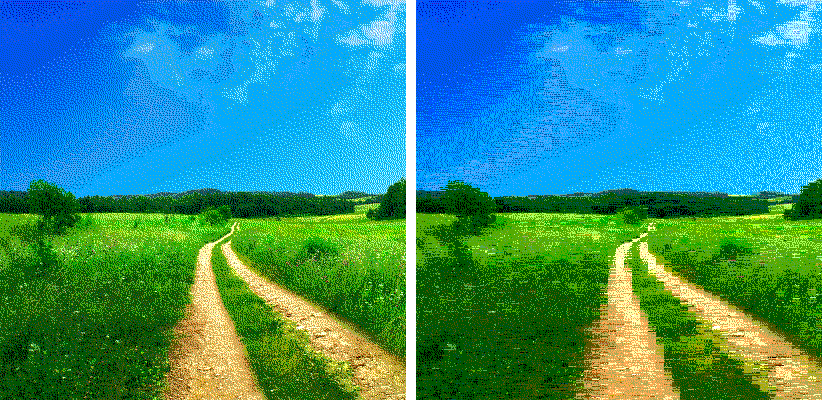
\includegraphics[width=0.9\columnwidth]{../figs/colour-restrictions.png}%
  \caption[Effect of colour constraints]{\label{fig:colour-constraints}The
    effect of the 8×1 colour constraint on graphics modes (640×480, in this
    case). Left, a 64-colour dithered test image, impossible to produce on the
    VDU. Right, the same image with 8×1 colour restrictions, as displayed by
    the VDU.}
\end{figure}


%\subsubsection{Graphics Modes}


%% %\begin{table}
%% \newcommand\vdumodePract[4]{%
%% %                   1       2                   3
%% %\vdumodeImpract{1}{16}{640×25 Graphics}{2 colours per 8×1 pixels.}
%% %\vdumodePract{4}{2}{160×200 Semigraphics}{C-plane. No restrictions.}
%% \bfseries{#3} & \bfseries{{#1}×{#2}} & \bfseries{#4}  \\ %
%% }
%% \newcommand\vdumodeImpract[4]{%
%% #3 & {{#1}×{#2}}%\tikz{\draw[fill=black,scale=0.01](0,0) rectangle (#1, #2); }
%% & #4  \\ %
%% }
%% %\caption{\label{table-vdu-modes}VDU Display modes.}
%% \vspace{1em}
%% \centering
%% \zebrarow{10}
%% \begin{longtable}{lll}
%%   %
%%   % First header
%%   %
%%   \hiderowcolors
%%   Mode & Cell & Description \\
%%   \hline
%%   \noalign{\global\rownum 0\relax}\showrowcolors
%%   \endfirsthead
%%   %
%%   % Subsequent headers
%%   %
%%   \hiderowcolors
%%   \noalign{\smallskip\smallskip}
%%   \multicolumn{3}{l}{\em Continued from previous page.}\\
%%   Mode & Cell & Description \\
%%   \hline
%%   \noalign{\global\rownum 1\relax}\showrowcolors
%%   \endhead
%%   %
%%   % Footer
%%   %
%%   \hiderowcolors
%%   \hline
%%   \noalign{\smallskip\smallskip}
%%   \multicolumn{3}{l}{\em Continued on next page.}\\
%%   \endfoot
%%   %
%%   % Last footer
%%   %
%%   \hiderowcolors
%%   \hline
%%   \endlastfoot
%%   %
%%   % Content
%%   %
%%   \showrowcolors
%%   \hline
%%   \input{../generated/mode-table}
%% \end{longtable}
%% %\end{table}

\begin{figure}
 \centering
 \inputfigure{figure-vdu-video-modes}
 \caption[Video Modes]{\label{fig:video-modes} Video mode chart showing the 34
   available modes (5×5, plus 5 80-column multicolour modes, plus four text
   modes). Unshaded modes are impractical due to the aspect ratio of the
   pixels. Multicolour and semi-graphics modes have no colour
   restrictions. Graphics modes allow two colours per 8×1 pixel block.}
\end{figure}




\section{Useful Display Mode Types}

The set of available display modes is a permutation of a number of options:

\begin{itemize}
  \item Whether the display intent is text or graphics.
  \item Whether 40 or 80 column mode is used.
  \item Whether 16, 8, 4, 2 or 1-line characters are used.
  \item Which block style is used: full-block, two-column block, or eight-column block.
\end{itemize}

Although this technically implies dozens of modes are possible, and all are
allowed by the hardware, many of these modes are:

\begin{itemize}
\item Of no use. For instance, text modes with 2-line characters are no good for text display.
\item Impractical. The 40×480 Multicolour and 640×30 Graphics modes are
  perfectly valid but their pixel shapes are too wide and too tall (respectively) for use.
\item Overshadowed by better modes. A 80×60 Semigraphics mode which only
  allows 2 colours per 4 horizontal pixels is valid, but the 80×60
  Multicolour mode offers the same resolution, no colour restrictions, and
  faster pixel access.
\end{itemize}

\begin{figure*}
  \centering
  \includegraphics[width=0.48\columnwidth]{../generated/vdu-test-image3-small-dithered-40x480MC.png}
  \ifxetex
    \hfill
  \else
    \vspace{1em}\\
  \fi
  \includegraphics[width=0.48\columnwidth]{../generated/vdu-test-image3-small-dithered-640x30HGR.png}%
  \caption[Two examples of impractical
    modes]{\label{fig:vdu:impractical-modes}Two examples of impractical
    modes. \ifxetex Left\else Top\fi, 40×480. \ifxetex Left\else Bottom\fi, 640×30.
    The pixel aspect ratios are too extreme
    for regular use, although the modes are accepted by the hardware. It should
    be noted that some computers from the past featured similarly extreme
    modes.}
\end{figure*}


\subsection{Mode Demonstrations}

The following pages demonstrate in practical terms what is capable in some of
the graphics modes. The original, unprocessed image is shown
in~\fcf{fig:vdu:original}, followed by renderings in progressively higher
resolution modes. To improve the quality, the image colour-space was quantised
from 8 bits per channel (16,777,216 colours) to 2 bits per channel (64
colours), with the error diffused using the Floyd-Steinberg dithering
algorithm.

\ifxetex
  \begin{figure}
    \centering
    
\includegraphics[width=0.9\columnwidth]{figs/vdu-test-image3-original.png}%
    \caption[Original 640×480 demonstration image]
            {\label{fig:vdu:mode-original}The original true-colour (24-bit colour)
      demonstration image, scaled down to 640×480.
    }
  \end{figure}
  
  \begin{figure}[p]
    \centering
    \includegraphics[width=0.9\columnwidth]{../generated/vdu-test-image3-small-dithered-40x30MC.png}%
    \caption[40×30 Multicolour mode]
            {\label{fig:vdu:mode-40x30mc}The 40×30 Multicolour mode.
              Each block can have its own independent colour.
              This is the same as the 40×30 text mode with whole-cell block graphics.
    }
  \end{figure}
  
  \begin{figure}[p]
    \centering
    \includegraphics[width=0.9\columnwidth]{../generated/vdu-test-image3-small-dithered-80x30MC.png}%
    \caption[80×30 Multicolour mode]{\label{fig:vdu:mode-80x30mc}The 80×30 Multicolour mode.
      Each block can have its own independent colour.
      This is the same as the 80×30 text mode with whole-cell block graphics.
    }
  \end{figure}
  
  
  \begin{figure}[p]
    \centering
    \includegraphics[width=0.9\columnwidth]{../generated/vdu-test-image3-small-dithered-80x60MC.png}%
    \caption[80×60 Multicolour mode]{\label{fig:vdu:mode-80x60mc}The 80×60 Multicolour mode.
      Each block can have its own independent colour.
      This is the same as the text mode with whole-cell block graphics.
    }
  \end{figure}
  
  \begin{figure}[p]
    \centering
    \includegraphics[width=0.9\columnwidth]{../generated/vdu-test-image3-small-dithered-160x60MC.png}%
    \caption[160×60 Semigraphics mode]{\label{fig:vdu:mode-160x60}The 160x60 Semigraphics mode.
      Each block can have its own independent colour.
    }
  \end{figure}
  
  \begin{figure}[p]
    \centering
    \includegraphics[width=0.9\columnwidth]{../generated/vdu-test-image3-small-dithered-160x120MC.png}%
    \caption[160×120 Semigraphics mode]{\label{fig:vdu:mode-160x120mc}The 160x120 Semigraphics mode.
      Each block can have its own independent colour.
    }
  \end{figure}
  
  \begin{figure}[p]
    \centering
    \includegraphics[width=0.9\columnwidth]{../generated/vdu-test-image3-small-dithered-160x240MC.png}%
    \caption[160×240 Semigraphics mode]{\label{fig:vdu:mode-160x240mc}The 160x240
      Semigraphics mode.  Each block can have its own independent colour.}
  \end{figure}
  
  \begin{figure}[p]
    \centering
    \includegraphics[width=0.9\columnwidth]{../generated/vdu-test-image3-small-dithered-320x240HGR.png}%
    \caption[320×240 Graphics mode]{\label{fig:vdu:mode-320x240hgr}The 320x240
      Graphics mode.  Two colours are allowed per 8×2 pixel block.  The colour
      restrictions cause obvious artifacts where numerous colours come close
      together.  }
  \end{figure}
  
  
  \begin{figure}[p]
    \centering
    \includegraphics[width=0.9\columnwidth]{../generated/vdu-test-image3-small-dithered-320x480HGR.png}%
    \caption[320×480 Graphics mode]{\label{fig:vdu:mode-320x480hgr}The 320x480 Graphics mode.
      Each block of 8×1 pixels can have its own independent colour.
      The colour restrictions cause obvious artifacts where numerous colours come close together.
      Higher vertical resolution alleviates some of this problem, but not in all cases.
    }
  \end{figure}
  
  
  \begin{figure}
    \centering
    \includegraphics[width=0.9\columnwidth]{../generated/vdu-test-image3-small-dithered-640x480HGR.png}%
    \caption[640×480 Graphics mode]{\label{fig:vdu:mode-640x480hgr}The 640x480 Graphics mode.
      Each block of 8×1 pixels can have its own independent colour.
      The colour restrictions cause obvious artifacts where numerous colours come close together.
      This is the highest spatial resolution available.
    }
  \end{figure}

\else

  \HCode{<div id="modeDemo" class="interactive widget"></div>}
  \HCode{<script type="text/javascript">}
  \HCode{$(document).ready(function(){makeModeDemoWidget();});} %$
  \HCode{</script>}

\fi




\section{Programming Model}

The following section discusses the software-side operation of the VDU board,
all of which is done via I/O space registers. There are thirteen registers in five groups.

\begin{enumerate}
  \item Registers configuring the entire display. In split screen mode, these
    registers configure the top portion of the split. The first register
    (\port{MCR0}) is also responsible for enabling video output and configuring
    interrupts, and serves as a detection and status register.
  \item Registers configuring the bottom portion of the split, in split screen
    mode. The first register (\port{MCR1}) is also responsible for enabling and
    configuring split-screen mode.
  \item Hardware cursor control registers.
  \item The PS/2 Keyboard register.
  \item Host interface registers.
\end{enumerate}



\begin{figure}
 \centering
 \inputfigure{figure-vdu-register-file}
 \caption[Register File]{\label{fig:vdu-register-file} Register File.}
\end{figure}




\subsection{Registers Controlling the Display}

\begin{ioport}{VDU}{1F0}{--wvehf}{MCR0}{Mode Control Register 0}

  This register controls whether or not the VDU card is enabled, configures
  interrupts, selects an appropriate character set and configures the display
  mode.

  \begin{bitfield}
    \bitfieldItem{3}{cfthl!50}{CRH}
    \bitfieldItem{1}{cfthl!25}{C40}
    \bitfieldItem{2}{cfthl!50}{CS2}
    \bitfieldItem{1}{cfthl!25}{VSI}
    \bitfieldItem{1}{cfthl!50}{SCI}
    \bitfieldItem{1}{cfthl!25}{VRI}
    \bitfieldItem{1}{cfthl!50}{KBI}
    \bitfieldRepConst{5}{0}
    \bitfieldItem{1}{cfthl!25}{EN}
  \end{bitfield}

  \begin{description}
    \li{\field{CRH}} is a three bit field that controls the height of the rows
    of character cells in scanlines. This in turn sets the vertical resolution
    in rows. Valid values are:
    
    \begin{description}
      \li{\bin{000}}: 16 lines per row, 30-row modes.
      \li{\bin{001}}: 8 lines per row, 60-row modes.
      \li{\bin{010}}: 4 lines per row, 120-pixel modes.
      \li{\bin{011}}: 2 lines per row, 240-pixel modes.
      \li{\bin{100}}: 1 line per row, 480-pixel modes.
      \li{\bin{101}}: Reserved, do not use.
      \li{\bin{11X}}: Reserved, do not use.
    \end{description}
    
    \li{\field{C40}} is a single bit flag. Set to \bin{1}, it enables
    40-column (320 pixel) wide modes. Set to \bin{0}, it specifies 80-column
    (640 pixel) modes.
    
    \li{\field{CS2}} is a two-bit quanity. It corresponds to bits 14 and 15
    of the character generator address and is used to set which character set
    of four is used in the current mode:
    
    \begin{description}
      \li{\bin{00}}: \hex{0000}–\hex{3FFF}.
      \li{\bin{01}}: \hex{4000}–\hex{7FFF}.
      \li{\bin{10}}: \hex{8000}–\hex{BFFF}.
      \li{\bin{11}}: \hex{C000}–\hex{FFFF}.
    \end{description}
    
    \li{\field{VSI}} controls the Vertical Sync Interrupt. If this bit is set,
    an interrupt will be signalled when vertical blanking begins. The processor
    can then modify the VDU image with minimum flickering, perhaps to implement
    a double-buffering technique. This flag defaults to \bin{0} when the system
    is reset.
    
    \li{\field{SCI}} controls the Split Count Interrupt. If this bit is set, an
    interrupt will be signalled whenever the scanline specified in \field{SCL}
    (see below) is being output. The interrupt is generated even when split
    screen mode is disabled. This flag defaults to \bin{0} when the system is reset.

    \li{\field{VRI}} controls the VDU Ready Interrupt. If this bit is set, an
    interrupt will be signalled at the completion of every host command.  This
    flag defaults to \bin{0} when the system is reset.

    \li{\field{KBI}} controls the Keyboard Interrupt. If this bit is set, an
    interrupt will be signalled whenever the keyboard has completed
    transmitting a byte of information. This flag defaults to \bin{0} when the
    system is reset.

    \li{\field{EN}} controls whether or not the VDU card is enabled. This
    flag defaults to \bin{0} when the system is reset. It must be set
    explicitly to enable display output.

  \end{description}

\end{ioport}



\begin{ioport}{VDU}{1F0}{-r-vehf}{SR}{Status Register}

  This read-only register shares its location with the \port{MCR0} register and
  mirrors some of the information stored it in. It is used for autodetection of
  the VDU card, and to detect the source of an interrupt.

  \begin{bitfield}
    \bitfieldItem{3}{cfthl!50}{CRH}
    \bitfieldItem{1}{cfthl!25}{C40}
    \bitfieldItem{2}{cfthl!50}{CS2}
    \bitfieldItem{1}{cfthl!25}{VSIS}
    \bitfieldItem{1}{cfthl!50}{SCIS}
    \bitfieldItem{1}{cfthl!25}{VRIS}
    \bitfieldItem{1}{cfthl!50}{KBIS}
    \bitfieldItem{5}{cfthl!50}{Version}
    \bitfieldItem{1}{cfthl!25}{EN}
  \end{bitfield}

  \begin{description}
    \li{\field{CRH}} contains the same value as the \field{CRH} field in the
    \port{MCR0} register.

    \li{\field{C40}} contains the same value as the \field{C40} field in the
    \port{MCR0} register.

    \li{\field{CS2}} contains the same value as the \field{CS2} field in the
    \port{MCR0} register.

    \li{\field{VSIS}} is set if a Vertical Sync Interrupt has been signalled
    since the last read of the \port{SR} register. This bit is cleared after
    the register is read.

    \li{\field{SCIS}} is set if a Split Count Interrupt has been signalled
    since the last read of the \port{SR} register. This bit is cleared after
    the register is read.

    \li{\field{VRIS}} is set if a VDU Ready Interrupt has been signalled since
    the last read of the \port{SR} register. This bit is cleared after the
    register is read.

    \li{\field{KBIS}} is set if a Keyboard Interrupt has been signalled since
    the last read of the \port{SR} register. Unlike other interrupt status
    bits, reading the \port{SR} does {\em not\/} clear this bit. This is done
    by reading the \port{KBD} register instead.

    \li{\field{Version}} is the version of the VDU card. For current revisions
    of the VDU, this field should yield the value \bin{00101}. This may be used
    to autodetect the presence of the card.

    \li{\field{EN}} matches the bit of the same name in the
    \port{MCR0} register. It is set if video generation is enabled. If
    clear, the VDU clocks are stopped and the output remains
    blanked. Most monitors will enter power saving mode within a few
    seconds of this happening.
  \end{description}

\end{ioport}






\begin{ioport}{VDU}{1F1}{--wvehf}{MCR1}{Mode Control Register 1}

  This register controls horizontal split mode, which allows the screen to be
  split in two. One display mode is shown in the top portion, another in the
  bottom portion. Each portion can act independently of the other so that
  scrolling graphics may be displayed in one portion, and text in the other.

  \begin{bitfield}
    \bitfieldItem{3}{cfthl!50}{CRH}
    \bitfieldItem{1}{cfthl!25}{C40}
    \bitfieldItem{2}{cfthl!50}{CS2}
    \bitfieldConst{0}
    \bitfieldGroup{1}{cfthl!25}{SEN}
    \bitfieldItem{8}{cfthl!50}{SCL}
  \end{bitfield}

  \begin{description}
    \li{\field{CRH}} is a three bit field that controls the bottom mode's
    cell row height setting controls the height of the rows of character cells
    in scanlines. It accepts the same values as the \field{CRH} field in the
    \port{MCR0} register.
    
    \li{\field{C40}} is a single bit flag. Set to \bin{1}, it enables
    40-column (320 pixel) wide modes in the bottom portion of the frame. Set
    to \bin{0}, it specifies 80-column (640 pixel) modes.

    \li{\field{CS2}} is a two-bit quanity. It corresponds to bits 14 and 15
    of the character generator address and is used to set the character set
    used in the bottom portion of the frame. It works exactly like the
    \field{CS2} field in the \port{MCR0} register.

    \li{\field{SEN}} when set to \bin{1}, enables split-screen mode.

    \li{\field{SCL}} this 8-bit value controls the scanline of the partition
    between top and bottom screen portions. This field is 8-bits wide while
    scanlines are 9 bits wide. Because of this, the split can be positioned
    with an accuracy of two scanlines. The scanline comparison includes the
    blanked lines, so the number must be offset. To place the split on line
    $n$, set \field{SCL} to $\lfloor\frac{n}{2}\rfloor+4$. For example, a value
    of 124 would put the split on the 240th scanline. If either of the modes is
    a text mode, it would help for the split to happen at a multiple of the
    tallest cell height so the split results in whole rows. Usually, this
    multiplier will be 16 or 8.
  \end{description}
\end{ioport}

\todo {The SCL formula above may be wrong. Verify}



\begin{ioport}{VDU}{1F2}{--wvehf}{SCR0}{Smooth Scroll Register 0}

  This register controls smooth scrolling in the horizontal and vertical
  direction. It applies to the top portion of the screen (or the entire screen,
  if split screen is disabled). It is eight bits wide, with the remaining bits
  set to \bin{0} to facilitate future expansion:

  \begin{bitfield}
    \bitfieldGroup{3}{cfthl!50}{HSCR}
    \bitfieldConst{0}
    \bitfieldGroup{4}{cfthl!50}{VSCR}
    \bitfieldRepConst{8}{0}
  \end{bitfield}

  \begin{description} \li{\field{HSCR}} shifts the displayed image left by a
    number of pixels. A value of \hex{0} does not shift the image; a value
    of \hex{7} shifts it to the left by seven pixels. This represents the range
    of modulo 8 and allows smooth scrolling to be implemented in conjunction
    with the \port{SAR0} register (which can shift in multiples of eight
    pixels).

    \li{\field{VSCR}} shifts the displayed image up by a number of
    pixels. A value of \hex{0} does not shift the image; a value of
    \hex{15} shifts it up by fifteen pixels. This represents the range
    of modulo 16 and allows smooth scrolling to be implemented in
    conjunction with the \port{SAR0} register. Please note that,
    depending on the current mode, the row field of \port{SAR0} can
    shift by 16, 8, 4, 2 or single pixels (30, 60, 120, 240 and 480
    line modes respectively), so the steps needed for smooth vertical
    scrolling depend on the mode.
  \end{description}

\end{ioport}


\begin{ioport}{VDU}{1F3}{--wvehf}{SCR1}{Smooth Scroll Register 1}

  This register controls smooth scrolling in the horizontal and vertical
  direction. It applies to the bottom portion of the screen, when split screen
  is enabled. Like \port{SCR0}, this register is eight bits wide, with the
  remaining bits set to \bin{0} to facilitate future expansion:

  \begin{bitfield}
    \bitfieldGroup{3}{cfthl!50}{HSCR}
    \bitfieldConst{0}
    \bitfieldGroup{4}{cfthl!50}{VSCR}
    \bitfieldRepConst{8}{0}
  \end{bitfield}

  \begin{description} \li{\field{HSCR}} shifts the displayed image left by a
    number of pixels. A value of \hex{0} does not shift the image; a value
    of \hex{7} shifts it to the left by seven pixels. This represents the range
    of modulo 8 and allows smooth scrolling to be implemented in conjunction
    with the \port{SAR1} register (which can shift in multiples of eight
    pixels).

    \li{\field{VSCR}} shifts the displayed image up by a number of
    pixels. A value of \hex{0} does not shift the image; a value of
    \hex{15} shifts it up by fifteen pixels. This represents the range
    of modulo 16 and allows smooth scrolling to be implemented in
    conjunction with the \port{SAR1} register. Please note that,
    depending on the current mode, the row field of \port{SAR1} can
    shift by 16, 8, 4, 2 or single pixels (30, 60, 120, 240 and 480
    line modes respectively), so the steps needed for smooth vertical
    scrolling depend on the mode.
  \end{description}

\end{ioport}


\begin{ioport}{VDU}{1F4}{--wvehf}{SAR0}{Start Address Register 0}

  This register sets the address in the video RAM of the top-left corner of the
  screen. It applies to the top portion of a split screen, or the entire screen
  if the split is not enabled.

  \begin{bitfield}
    \bitfieldGroup{7}{cfthl!50}{Column}
    \bitfieldGroup{9}{cfthl!25}{Row}
  \end{bitfield}

  \begin{description}
  \li{\field{Column}} The column address of the top left cell on the screen.
  \li{\field{Row}} The row address of the top left cell on the screen.
  \end{description}

\end{ioport}






\begin{ioport}{VDU}{1F5}{--wvehf}{SAR1}{Start Address Register 1}

  This register sets the address in the video RAM of the top-left corner of the
  screen. It applies to the bottom portion of a split screen.

  \begin{bitfield}
    \bitfieldGroup{7}{cfthl!50}{Column}
    \bitfieldGroup{9}{cfthl!25}{Row}
  \end{bitfield}

  \begin{description}
  \li{\field{Column}} The column address of the top left cell of the bottom half of a split-screen setup.
  \li{\field{Row}} The row address of the top left cell of the bottom half of a split-screen setup.
  \end{description}

\end{ioport}




\begin{ioport}{VDU}{1F6}{--wvehf}{MAR0}{Modulo Address Register 0}

  This register sets the modulo address. It applies to the top portion of a
  split screen, or the entire screen if the split is not enabled. The effects
  of modulo address registers are described in~\cf{vdu:sec:modulo-address}.

  \begin{bitfield}
    \bitfieldGroup{7}{cfthl!50}{Column}
    \bitfieldGroup{9}{cfthl!25}{Row}
  \end{bitfield}

  \begin{description}
  \li{\field{Column}} The column modulo address of the screen.
  \li{\field{Row}} The row modulo address of the screen.
  \end{description}

\end{ioport}






\begin{ioport}{VDU}{1F7}{--wvehf}{MAR1}{Modulo Address Register 1}

  This register sets the modulo address. It applies to the bottom portion of a
  split screen. The effects of modulo address registers are described
  in~\cf{vdu:sec:modulo-address}.

  \begin{bitfield}
    \bitfieldGroup{7}{cfthl!50}{Column}
    \bitfieldGroup{9}{cfthl!25}{Row}
  \end{bitfield}

  \begin{description}
  \li{\field{Column}} The column modulo address of the bottom half of a split-screen setup.
  \li{\field{Row}} The row modulo address of the bottom half of a split-screen setup.
  \end{description}

\end{ioport}




\begin{ioport}{VDU}{1F8}{--wvehf}{CCR}{Cursor Control Register}

  This register controls the appearance and behaviour of the hardware
  cursor. The cursor's behaviour is described in~\cf{sec:vdu:cursor}.

  \begin{bitfield}
    \bitfieldGroup{6}{cfthl!50}{Foreground}
    \bitfieldGroup{2}{cfthl!25}{CBC}
    \bitfieldGroup{6}{cfthl!50}{Background}
    \bitfieldRepConst{2}{0}
  \end{bitfield}

  \begin{description}
    \li{\field{Foreground}} is the foreground \ds{Colour} of the character
    cell the cursor is on, when it is visible.
    \li{\field{CBC}} is the cursor blink control field. It controls the
    visibility and blink rate of the cursor:
    
    \begin{description}
      \li{\bin{00}} the cursor is always invisible (off).
      \li{\bin{01}} the cursor is always visible (on) and does not blink.
      \li{\bin{10}} the cursor is visible and blinking at double the rate of
      blinking text.
      \li{\bin{11}} the cursor is visible and blinking at the same rate and
      in phase with blinking text.
    \end{description}
    
    \li{\field{Background}} is the background \ds{Colour} of the character
    cell the cursor is on, when it is visible.
  \end{description}

\end{ioport}

\begin{ioport}{VDU}{1F9}{--wvehf}{CAR}{Cursor Address Register}

  This register sets the location of the cursor. The cursor will be visible
  (according to the settings of the \port{CCR} register when the specified
  address is displayed. This implies that the cursor may be off-screen and thus
  invisible. This provides a second way of hiding the cursor (in addition to
  disabling it via the \field{CBC} field in the \port{CCR} register). The
  cursor's full behaviour is described in~\cf{sec:vdu:cursor}.

  \begin{bitfield}
    \bitfieldGroup{7}{cfthl!50}{Cursor Column} The column address of the cursor's location.
    \bitfieldGroup{9}{cfthl!25}{Cursor Row} The row address of the cursor's location.
  \end{bitfield}

\end{ioport}


\subsection{Registers Controlling the Keyboard}

The VDU board contains an optional PS/2 keyboard interface operated by the
\field{KBI} bit in the \port{MCR0} register, the \field{KBIS} in the \port{SR}
register, and the \port{KBD} register, described below. The keyboard interface
is described in detail in~\ccf{chap:kbd}.

\begin{ioport}{VDU}{1FB}{-rwvehf}{KBD}{Keyboard Register}

  This register operates the PS/2 keyboard interface. A full description of
  this interface can be found in~\ccf{chap:kbd}.

  \begin{bitfield}
    \bitfieldGroup{8}{cfthl!25}{Keyboard Data}
    \bitfieldGroup{1}{cfthl!50}{KDP}
    \bitfieldRepConst{4}{0}
    \bitfieldGroup{1}{cfthl!25}{KC}
    \bitfieldGroup{1}{cfthl!50}{KD}
    \bitfieldGroup{1}{cfthl!25}{KDR}
  \end{bitfield}

  \begin{description}
    \li{\field{Keyboard Data}} is a read-only 9-bit value as transmitted by the
    keyboard. The ninth bit (\field{KDP}) is an odd parity bit. It is clear if
    there is an odd number of set bits in the remaining 8 bits, otherwise it is
    set.  \li{\field{KC}} is a direct connection to the keyboard clock
    pin. When reading, the keyboard clock pin will be sampled directly. Writing
    to this bit controls the clock driver. Clearing the bit drives the clock
    line low. Setting it releases the clock line, allowing the keyboard to
    operate. Setting this bit thus allows the keyboard to be inhibited
    programmatically. Setting, then clearing this bit sends a clock pulse to
    the keyboard. Writing to the \port{KBD} register does not change the value
    of this field.

    \li{\field{KD}} is a direct connection to the keyboard data pin. \field{KD}
    and \field{KC} may be used to manually read from the keyboard, one bit at a
    time. When writing to \field{KD}, setting the bit drives the data line
    low. Clearing it releases the data line, allowing it to be pulled up to a
    high state. \field{KD} may be used to send data to the keyboard. The data
    bits must be complemented by the host prior to sending, and the host is
    also responsible for transmitting correct start, parity and stop bits and
    operating the clock line at sufficiently slow rates.

    \li{\field{KDR}} is set if a full byte of keyboard data has been received
    and is ready for processing. After reading from \port{KBD}, if \field{KDR}
    is set, it will be cleared and the keyboard receiver reset. The keyboard
    inhibit condition will be removed and the keyboard will be free to transmit
    another byte when it needs to. The interrupt status bit \field{KBIS} is
    also cleared at this time.
  \end{description}
\end{ioport}




\subsection{Manipulating the Display Memory}

Manipulating the video memory is also performed indirectly, by communicating
with the VDU using an extended instruction (or command register), and three
registers.

\begin{ioport}{VDU}{1FA}{-rwvehf}{HAR}{Host Address Register}

  This read/write register contains the address of the next location to be read
  from or written to by the CFT host. 

  Reading from or writing to this register will generate wait states until or
  unless the VDU's host interface is idle (i.e. any previous command has
  executed fully and \port{CRR}, as well as \field{GO} in \field{CMD} are both
  zero). Reading from the \port{HAR} register is thus a good way to block
  execution while the VDU is running a command.

  \begin{bitfield}
    \bitfieldGroup{7}{cfthl!50}{Column}
    \bitfieldGroup{9}{cfthl!25}{Row}
  \end{bitfield}

\end{ioport}



\begin{ioport}{VDU}{1FD}{-rwvehf}{CRR}{Command Repetition Register}

  The CRR is a 9-bit read-write register. Setting it to a non-zero value prior
  to issuing a host command causes the host command to repeat $\mbox{CRR}+1$
  times. That is, a value of \hex{000} denotes one repetition, and a value of
  \hex{1FF} denotes 512 repetitions. This makes it possible to operate on
  entire rows or columns of the video memory, depending on the command.

  The register is decremented by the VDU engine while commands are being
  executed, and may be used to monitor repeated command progress. When the VDU
  host interface has completed its command, CRR will contain \hex{000}, and the
  \field{GO} field in the \port{CMD} register will be set. Further commands
  will only execute once because of the \hex{000} value.

  \begin{bitfield}
    \bitfieldGroup{9}{cfthl!50}{Repetitions}
    \bitfieldRepConst{7}{0}
  \end{bitfield}

  Only the least significant nine bits are in use at this location. All other
  bits are ignored on writes, and reads return \bin{0000000} for the most
  significant seven bits.

  Reading from this register is one way of polling for command completion, but
  only for the completion of a repeated command. To poll the completion of any
  command, check the \field{GO} field in the \port{CMD} register.

  Writing to this register will generate wait states until or unless the VDU's
  host interface is idle.

\end{ioport}


\begin{ioport}{VDU}{1FE}{-rwvehf}{CPORT}{C Plane Register}

  This read/write register contains data retrieved from the C plane, or to be written to
  the C plane. It is 16 bits wide and follows the layout of the C plane itself:

  \begin{bitfield}
    \bitfieldGroup{6}{cfthl!50}{Foreground}
    \bitfieldGroup{2}{cfthl!25}{CS1}
    \bitfieldGroup{6}{cfthl!50}{Background}
    \bitfieldGroup{1}{cfthl!25}{INV}
    \bitfieldGroup{1}{cfthl!25}{BLN}
  \end{bitfield}

  \begin{description}
    \li{\field{Foreground}} is the foreground \ds{Colour} of the
    corresponding character in the B Plane.
    \li{\field{CS1}} is a two-bit quanity. It corresponds to bits 12 and 13
    of the character generator address and is used to set which character set
    is used by the corresponding character in the B plane. Field \field{CS2} in
    either \port{MCR0} or \port{MCR1} provides bits 14 and 15. The character
    itself provides the remaining 12 bits (256 characters, 16 lines each).
    \li{\field{Background}} is the background \ds{Colour} of the character
    cell corresponding to this value.
    \li{\field{INV}} is the ‘inverse video’ attribute. When this bit is
    \bin{1}, the foreground and background colours specified here are
    swapped. Inverse video is used to highlight text.
    \li{\field{BLN}} is the ‘blink’ attribute. When this bit is \bin{1}, the
    foreground colour is periodically set to be the foreground colour. This
    makes foreground pixels disappear and reappear periodically, causing them
    to blink. The blink frequency is 2.3Hz.
  \end{description}

  Reading from or writing to this register will generate wait states until or unless the VDU's
  host interface is idle (i.e. any previous command has executed fully and
  \port{CRR} is zero). 

\end{ioport}


\begin{ioport}{VDU}{1FF}{crwvehf}{CMD/BPORT/CGPORT}{Command, B Plane port, CG RAM port Register}

  This read/write register combines read/write access to the B Plane
  and Character Generator RAM, and supplies the VDU card with host
  interface commands and their options.

  \begin{bitfield}
    \bitfieldGroup{8}{cfthl!50}{B/CG Data}
    \bitfieldGroup{1}{cfthl!25}{XINC}
    \bitfieldItem{1}{cfthl!50}{YINC}
    \bitfieldGroup{4}{cfthl!25}{Command}
    \bitfieldRepConst{1}{0}
    \bitfieldItem{1}{cfthl!50}{GO}
  \end{bitfield}

  \begin{description}
    \li{\field{B/CG Data}} holds data read from or about to be written to the
    B plane, or data about to be written to the Character Generator RAM.
    
    \li{\field{XINC}} if set to \bin{1}, the column address of the \port{HAR}
    will be incremented by one after the command runs.
    
    \li{\field{YINC}} if set to \bin{1}, the row address of the \port{HAR}
    will be incremented by one after the command runs (i.e. the \port{HAR} will
    be incremented by 128).
    
    \li{\field{Command}} identifies the operation to be performed. The
    following commands are available:
    \begin{description}
      \li{\bin{0000}} Write to B and C planes.
      \li{\bin{0001}} Write to B plane.
      \li{\bin{0010}} OR value with B plane value, write to C plane.
      \li{\bin{0011}} OR value with B plane value.
      \li{\bin{0100}} Mask (AND) value with B plane value, write to C plane.
      \li{\bin{0101}} Mask (AND) value with B plane value.
      \li{\bin{0110}} Toggle (XOR) value with B plane value, write to C plane.
      \li{\bin{0111}} Toggle (XOR) value with B plane value.
      %
      \li{\bin{1000}} Write to C plane only.
      \li{\bin{1011}} Write to Character Generator RAM.
      \li{\bin{1101}} Read from B and C planes.
      %
    \end{description}

    All other values are reserved for future expansion and should not be used.

    \li{\field{GO}} Must {\em always\/} be clear (\bin{0}) to start a
    command. Once the command has been executed, this bit is set to \bin{1}.
    This also happens if the command is one of the reserved opcodes.
  \end{description}

  These commands are explained in detail
  in~\cf{sec:vdu:using-host-iface}. Please note that incrementation of the
  \port{HAR} is not subject to the \port{MAR0}/port{MAR1} registers: though
  conventionally interpreted as a column/row vector register, this is really a
  16-bit scalar register incremented as a whole. X increments simply add the
  value \hex{0001} to the register, while Y increments add the value
  \hex{0080}.

  Writing to this register will generate wait states until or unless the VDU's
  host interface is idle (i.e. any previous command has executed fully
  and \port{CRR} is zero). Reading from the register does not introduce wait
  states, making this a good way to poll for command completion. Generating
  wait states on write (when busy) allows the processor to send the VDU a
  stream of commands without waiting for each command to complete.

\end{ioport}

\subsection{Using the Host Interface}
\label{sec:vdu:using-host-iface}

The indirect nature of the VDU-to-host interface makes it appear daunting at
first, but this complexity is a boon to the CFT programmer, since the VDU
offloads a significant amount of work.

The algorithm for writing data to the VDU is quite straightforward: first, and
optionally (the location may already be correct) set the location to write to
by writing its address to the \port{HAR}. If modifying colour information for
that location, set the \port{CPORT} register. If modifying multiple locations
at once, set the \port{CRR} register. Then, write a command and character (B
plane) data to \port{CMD}. Repeat as required. If the VDU isn't ready for a new
command yet, writing to the \port{HAR}, \port{CPORT} or \port{CRR} will block
execution with wait states.

The algorithm for reading data is simpler: write a command to \port{CMD}, then
read character (B plane) or character generator data from it. Optionally, also
read \port{CPORT} to get C plane data.

Below is a detailed list of all supported commands with suggested mnemonics and
values (in binary), as listed above.

\begin{description}
  \li{\textsf{WB} (\bin{0001)}: Write to B plane.} A single write to the B plane is
  performed, at the location in \port{HAR}, using data supplied in the
  \port{CMD} register. Colours and attributes are not modified. One memory
  write is performed.

  \li{\textsf{WBC} (\bin{0000}): Write to B and C planes.} Same as above, but in addition the
  value of the \port{CPORT} register is stored at the C plane location in
  \port{HAR}, modifying the colours and attributes of the current location. Two
  memory writes are performed.

  \li{\textsf{ORB} (\bin{0011}): OR value with B plane value.} The B plane value at the
  location in \port{HAR} is read, and ORred with the value in the \port{CMD}
  register. The result is written back to the same B plane location and is also
  made available in the \field{BPORT} field of \port{CMD}. Mostly useful for
  bitmap graphics, this command is ideal for setting individual pixels without
  having to perform host-side reads or \asm{OR} operations. One memory read and
  one memory write are performed.

  \li{\textsf{ORBWC} (\bin{0010}): OR value with B plane value, write to C plane.} Same as
  above, but in addition the value of the \port{CPORT} register is stored at
  the C plane location in \port{HAR}, modifying the colours and attributes of
  the current location. One memory read is performed, followed by
  two memory writes.

  \li{\textsf{ANDB} (\bin{0101}): Mask (AND) value with B plane value.} The B plane value at
  the location in \port{HAR} is read, and ANDed with the value in the
  \port{CMD} register. The result is written back to the same B plane location
  and is also made available in the \field{BPORT} field of \port{CMD}. Mostly
  useful for bitmap graphics, this command is ideal for clearing or masking
  individual pixels without having to perform host-side reads or \asm{AND}
  operations. As expected, the bitmap value to clear must be inverted with
  \asm{NOT} prior to this operation. One memory read and one memory write are
  performed.

  \li{\textsf{ANDBWC} (\bin{0100}): Mask (AND) value with B plane value, write to C plane.} Same
  as above, but in addition the value of the \port{CPORT} register is stored at
  the C plane location in \port{HAR}, modifying the colours and attributes of
  the current location. One memory read is performed, followed by
  two memory writes.

  \li{\textsf{XORB} (\bin{0111}): Toggle (XOR) value with B plane value.} The B plane value at
  the location in \port{HAR} is read, and XORed with the value in the
  \port{CMD} register. The result is written back to the same B plane location
  and is also made available in the \field{BPORT} field of \port{CMD}. Mostly
  useful for bitmap graphics, this command is ideal for toggling individual
  pixels without having to perform host-side reads or \asm{XOR}
  operations. This operation is useful for ‘rubber-bands’ or cursors, as
  performing it twice negates its effects. One memory read and one memory write
  are performed.

  \li{\textsf{XORBWC} (\bin{0110}): Toggle (XOR) value with B plane value, write to C plane.}
  Same as above, but in addition the value of the \port{CPORT} register is
  stored at the C plane location in \port{HAR}, modifying the colours and
  attributes of the current location. One memory read is performed, followed by
  two memory writes.

  \li{\textsf{WC} (\bin{1000}): Write to C plane only.} The value of the \port{CPORT}
  register is stored at the C plane location in \port{HAR}, modifying the
  colours and attributes of the current location without changing character or
  bitmap data. This command is useful for multicolour modes, or for simply
  painting over B plane data with colour. One memory write is performed.

  \li{\textsf{WCG} (\bin{1011}): Write to Character Generator RAM.} The value of the
  \field{CGPORT} field in the \port{CMD} register is written to the Character
  Generator RAM position in \port{HAR}, modifying part of a character
  pattern. This instruction is used to update font data. One memory write is
  performed.

  \li{\textsf{RBC} (\bin{1101}): Read from B and C planes.} The 8-bit value at the B plane
  location in \port{HAR} is read into the \field{BPORT} field in the \port{CMD}
  register. The 16-bit value at the C plane location in \port{HAR} is read into
  the \port{CPORT} register. Two memory reads are performed.

  %
\end{description}

All other commands are reserved for future expansion and should not be used. If
requested, the VDU will perform no task and will return to the ready state
immediately, setting the \field{GO} bit in the \port{CMD} register.

After execution of each command, the value of \port{HAR} is incremented by
\hex{0001} if \field{XINC} is set in the \port{CMD} register, and by \hex{0080}
if \field{YINC} is set. Although this is of limited use, both may be specified,
which increments \port{HAR} by \hex{0081} (along the main diagonal).

Repeating commands with neither \field{XINC} not \field{YINC} set is,
naturally, pointless as the address does not change between iterations.


\subsection{Examples}

\subsubsection{Write a Character With Colour}

This is a complete example to write an arbitrary character with a particular
colour.

\begin{cftasmcode}
         LI &82                      ; coordinates (2,1) (2 + 1 * 128)
         OUT VDU HAR                 ; Set address
         LOAD colour                 ; Load the colour attribute
         OUT VDU CPORT               ; Set the colour attribute
         LOAD cmd                    ; Load command
         OR char                     ; OR the character
         OUT VDU CMD                 ; Initiate the command
         HALT

colour:  .word &003F                 ; white on black
char:    .word 65                    ; ASCII 65 ('A')
cmd:     .word #000:000:0:1:00000000 ; Command 000, XINC = 1
\end{cftasmcode}

\noindent The code to write subsequent characters with the same colour and attributes is
considerably simpler because of the address auto-increment and the persistence
of the \port{CPORT} register:

\begin{cftasmcode}
         LOAD cmd                    ; Load command
         OR char                     ; OR the character
         OUT VDU CMD                 ; Initiate the command
\end{cftasmcode}

\noindent This seems a little excessive for writing a single character, but given the
nature of CFT Assembly, it is actually shorter than doing the same thing on a
hypothetical, non-planar memory-mapped VDU card, where colours are stored in
even locations and characters in odd ones\footnote{Exactly the way it is done
  in MDA, CGA, EGA, MCGA and VGA text modes.}:

\begin{cftasmcode}
         LI &82                      ; coordinates (2,1) (2 + 1 * 128)
         SBL                         ; Multiply by two
         ADD baddr1                  ; Add VDU base address (attrs)
         STORE R &80                 ; Use an autoincrement register
         ADD baddr2                  ; Add VDU base address (chars)
         STORE R &81                 ; Use another autoinc register

         LOAD colour                 ; Load the colour attribute
         STORE I R &80               ; Store the attribute
         LOAD char                   ; Load the character
         STORE I R &81               ; Store it
         HALT

baddr1:  .word &a000                 ; Base addr (attrs)
baddr2:  .word &a001                 ; Base addr (chars)
colour:  .word &003F                 ; white on black
char:    .word 65                    ; ASCII 65 ('A')
\end{cftasmcode}

\noindent The downside on dumb, memory-mapped devices is that writing {\em subsequent\/}
characters still takes more instructions:

\begin{cftasmcode}
         LOAD colour                 ; Load the colour attribute
         STORE I R &80               ; Store the attribute
         LOAD char                   ; Load the character
         STORE I R &81               ; Store it
\end{cftasmcode}

\noindent With the limited intelligence of the VDU card, writing two characters
with their colour values took 13 words and 10 instructions, while a
memory-mapped VGA-like device would need 17 words and 14 instructions, ignoring
the \asm{HALT} instruction.



\subsubsection{Write Two Characters Without Modifying Colours}

This changes the B plane without changing the C plane, keeping the colours and
attributes intact. The only difference from the previous example is the command
used:

\begin{cftasmcode}
         LI &82                      ; coordinates (2,1) (2 + 1 * 128)
         OUT VDU HAR                 ; Set address
         LOAD cmd                    ; Load command
         OR char1                    ; OR the character
         OUT VDU CMD                 ; Initiate the command

         LOAD cmd                    ; Load command
         OR char2                    ; OR the character
         OUT VDU CMD                 ; Initiate the command
         HALT

char1:   .word 65                    ; ASCII 65 ('A')
char2:   .word 66                    ; ASCII 65 ('B')
cmd:     .word #000:001:0:1:00000000 ; Command 001, XINC = 1
\end{cftasmcode}


\subsubsection{Paint Colour Attributes Without Modifying Characters}

This changes the C plane without touching the B plane, keeping the characters
intact but changing the colours and attributes. Again, the only difference is
in the command used, but modifying four consecutive positions is quite simple:

\begin{cftasmcode}
         LI &82                      ; coordinates (2,1) (2 + 1 * 128)
         OUT VDU HAR                 ; Set address
         LOAD colour                 ; Set the colour
         OUT VDU CPORT
         LOAD repeats                ; Set the number of repetitions
         OUT VDU
         LOAD cmd                    ; Initiate the command
         OUT VDU CMD
         HALT

colour:  .word &3f00                 ; Black on white
repeats: .word 3                     ; Number of characters +1
cmd:     .word #000:010:0:1:00000000 ; Command 010, XINC = 1
\end{cftasmcode}



\subsubsection{Creating a New Character Pattern}

This changes the C plane without touching the B plane, keeping the characters
intact but changing the colours and attributes. Again, the only difference is
in the command used, but modifying four consecutive positions is quite simple:

\begin{cftasmcode}
         LI 65                       ; set the pattern for 'A'
         CLL RNL                     ; Multiply by 16
         OUT VDU HAR                 ; Set address
         LOAD pattern                ; Load start address of pattern
         STORE R &80                 ; Use an autoincrement register
         LI 16                       ; Loop 16 times
         NEG
         STORE R &10
loop:    LOAD I R &80                ; Load pattern data
         OR cmd
         OUT VDU CMD                 ; Send command and CG data
         ISZ R &10                   ; Loop?
         JMP loop
         HALT

cmd:     .word #000:011:0:1:00000000 ; Command 011, XINC = 1
pattern: .word #--------             ; Ascender, line 1
         .word #--------             ; Ascender, line 2
         .word #--------             ; Ascender, line 3
         .word #---1----             ; Top line of letters
         .word #--111---             ; 2
         .word #-11-11--             ; 3
         .word #11---11-             ; 4
         .word #11---11-             ; 5
         .word #1111111-             ; 6
         .word #1111111-             ; 7
         .word #11---11-             ; 8
         .word #11---11-             ; 9
         .word #11---11-             ; Bottom line of letters
         .word #--------             ; Descender, line 1
         .word #--------             ; Descender, line 2
         .word #--------             ; Descender, line 3
\end{cftasmcode}





\subsubsection{Read a Screen Row}

This example uses the read command to read all 128 cells of the first row of
the VDU memory. Both the B and C planes are read and stored in an interlaced
manner, suitable for writing to mass storage.

\begin{cftasmcode}
         LI 128                      ; Read 128 values
         NEG 
         STORE R &10
         LI 0                        ; Start address
         OUT VDU HAR                 ; Set it
         LOAD dest                   ; Get the destination
         STORE R &80                 ; Use an autoincrement register
         LOAD cmd
         OUT VDU CMD                 ; Issue the read command

loop:    IN VDU CPORT                ; First read from the C plane
         STORE I R &80               ; Store it
         IN VDU BPORT                ; Reading from the B PORT
                                     ; triggers the next read
         STORE I R &80
         ISZ R &10                   ; Loop?
         JMP loop
         HALT

source:  .word &0000                 ; Source VDU address
dest:    .word &8000                 ; Destination buffer
cmd:     .word #000:100:0:1:00000000 ; Command 100, XINC = 1
\end{cftasmcode}

\noindent Because of the way read increments are structured, to read the entire
display memory would require wrapping this code in an outer loop (which sets
the \port{HAR}) and up to 512 iterations.


\subsection{Suggested Mode Settings}

The following sections list suggested register values to configure various
useful modes, including some common variations. In all these samples, unless
stated otherwise, interrupt signalling is disabled and characters use character
set 0. The start address is reset to location \hex{0000}.

\subsubsection{80×30 Text/Semigraphics/Multicolour Mode}

This is the standard 80×30 text mode. After setting registers, the video memory
may be configured as a text, 160×30 semigraphics or 80×30 multicolour mode as
described in~\cf{sec:vdu:modes}. Of these, the text mode is the most useful.

\begin{center}
  \zebra
  \begin{tabular}{rccl}
    %\noalign{\smallskip}\hline\noalign{\smallskip}
    %\\\hline
    Address & Register & Value & Notes \\
    %\noalign{\smallskip}\hline\noalign{\smallskip}
    \hline
    \hex{1F0} & \hex{MCR0}  & \hex{8000} & Enable, 80 columns, 30 rows\\
    \hex{1F1} & \hex{MCR1}  & \hex{0000} & No split mode \\
    \hex{1F2} & \hex{SCR0}  & \hex{0000} & No smooth scroll \\
    \hex{1F4} & \hex{SAR0}  & \hex{0000} & Viewport origin at (0,0)\\
    \hex{1F6} & \hex{MAR0}  & \hex{FFFF} & Modulo at (127,511)\\
    \hex{1F8} & \hex{CCR}   & \hex{0B80} & Fast blinking orange cursor\\
    \hex{1F9} & \hex{CAR}   & \hex{0000} & Cursor at (0,0)\\
    \hex{1FA} & \hex{HAR}   & \hex{0000} & Next character at (0,0)\\
    \hex{1FD} & \hex{CPORT} & \hex{003F} & Set white on black for next character\\
    \hline
  \end{tabular}
\end{center}



\subsubsection{80×60 Text/Semigraphics/Multicolour Mode}

This is the 80×60 text mode, where character cells are 8×8, less legible than
the 8×16 of the corresponding 30-line mode. After setting registers, the video
memory may be configured as a text, 160×60 semigraphics or 80×60 multicolour mode
as described in~\cf{sec:vdu:modes}. The latter has square \glspl{PEL} and is
quite useful.

\begin{center}
  \zebra
  \begin{tabular}{rccl}
    %\noalign{\smallskip}\hline\noalign{\smallskip}
    %\\\hline
    Address & Register & Value & Notes \\
    %\noalign{\smallskip}\hline\noalign{\smallskip}
    \hline
    \hex{1F0} & \hex{MCR0}  & \hex{8011} & Enable, font 4, 80 columns, 60 rows\\
    \hex{1F1} & \hex{MCR1}  & \hex{0000} & No split mode \\
    \hex{1F2} & \hex{SCR0}  & \hex{0000} & No smooth scroll \\
    \hex{1F4} & \hex{SAR0}  & \hex{0000} & Viewport origin at (0,0)\\
    \hex{1F6} & \hex{MAR0}  & \hex{FFFF} & Modulo at (127,511)\\
    \hex{1F8} & \hex{CCR}   & \hex{0B80} & Fast blinking orange cursor\\
    \hex{1F9} & \hex{CAR}   & \hex{0000} & Cursor at (0,0)\\
    \hex{1FA} & \hex{HAR}   & \hex{0000} & Next character at (0,0)\\
    \hex{1FD} & \hex{CPORT} & \hex{003F} & Set white on black for next character\\
    \hline
  \end{tabular}
\end{center}


\subsubsection{40×30 Text/Semigraphics/Multicolour Mode}

This text mode is highly legible from a distance, and has square characters,
making it useful for games and graphics display. After setting registers, the
video memory may be configured as a text, 80×30 semigraphics or 40×30
multicolour mode as described in~\cf{sec:vdu:modes}. The latter has the largest
square \glspl{PEL} of any mode. The 80×30 semigraphics mode is not particularly
useful. The 80×30 multicolour is identical in features and easier to use.

\begin{center}
  \zebra
  \begin{tabular}{rccl}
    %\noalign{\smallskip}\hline\noalign{\smallskip}
    %\\\hline
    Address & Register & Value & Notes \\
    %\noalign{\smallskip}\hline\noalign{\smallskip}
    \hline
    \hex{1F0} & \hex{MCR0}  & \hex{8009} & Enable, 40 columns, 30 rows\\
    \hex{1F1} & \hex{MCR1}  & \hex{0000} & No split mode \\
    \hex{1F2} & \hex{SCR0}  & \hex{0000} & No smooth scroll \\
    \hex{1F4} & \hex{SAR0}  & \hex{0000} & Viewport origin at (0,0)\\
    \hex{1F6} & \hex{MAR0}  & \hex{FFFF} & Modulo at (127,511)\\
    \hex{1F8} & \hex{CCR}   & \hex{0B80} & Fast blinking orange cursor\\
    \hex{1F9} & \hex{CAR}   & \hex{0000} & Cursor at (0,0)\\
    \hex{1FA} & \hex{HAR}   & \hex{0000} & Next character at (0,0)\\
    \hex{1FD} & \hex{CPORT} & \hex{003F} & Set white on black for next character\\
    \hline
  \end{tabular}
\end{center}



\subsubsection{160×120 Semigraphics Mode}

The lowest 4:3-aspect graphics mode displays 160×120 \glspl{PEL}, each 4×4
native resolution pixels in size. There are no colour restrictions.

\begin{center}
  \zebra
  \begin{tabular}{rccl}
    %\noalign{\smallskip}\hline\noalign{\smallskip}
    %\\\hline
    Address & Register & Value & Notes \\
    %\noalign{\smallskip}\hline\noalign{\smallskip}
    \hline
    \hex{1F0} & \hex{MCR0}  & \hex{8002} & Enable, 80 columns, 120 rows\\
    \hex{1F1} & \hex{MCR1}  & \hex{0000} & No split mode \\
    \hex{1F2} & \hex{SCR0}  & \hex{0000} & No smooth scroll \\
    \hex{1F4} & \hex{SAR0}  & \hex{0000} & Viewport origin at (0,0)\\
    \hex{1F6} & \hex{MAR0}  & \hex{FFFF} & Modulo at (127,511)\\
    \hex{1F8} & \hex{CCR}   & \hex{0000} & Cursor off\\
    \hex{1F9} & \hex{CAR}   & \hex{0000} & Cursor off\\
    \hex{1FA} & \hex{HAR}   & \hex{0000} & Next character at (0,0)\\
    \hex{1FD} & \hex{CPORT} & \hex{003F} & Set white on black for next character\\
    \hline
  \end{tabular}
\end{center}


\subsubsection{320×240 Graphics Mode}

The lowest 4:3-aspect full graphics mode displays 320×240 \glspl{PEL}, each 2×2
native resolution pixels in size. It is based on the 40-column timings. As with
all graphics modes, every 8×1 PEL region can only have one foreground and one
background colour.

\begin{center}
  \zebra
  \begin{tabular}{rccl}
    %\noalign{\smallskip}\hline\noalign{\smallskip}
    %\\\hline
    Address & Register & Value & Notes \\
    %\noalign{\smallskip}\hline\noalign{\smallskip}
    \hline
    \hex{1F0} & \hex{MCR0}  & \hex{800C} & Enable, 40 columns, 240 rows\\
    \hex{1F1} & \hex{MCR1}  & \hex{0000} & No split mode \\
    \hex{1F2} & \hex{SCR0}  & \hex{0000} & No smooth scroll \\
    \hex{1F4} & \hex{SAR0}  & \hex{0000} & Viewport origin at (0,0)\\
    \hex{1F6} & \hex{MAR0}  & \hex{FFFF} & Modulo at (127,511)\\
    \hex{1F8} & \hex{CCR}   & \hex{0000} & Cursor off\\
    \hex{1F9} & \hex{CAR}   & \hex{0000} & Cursor off\\
    \hex{1FA} & \hex{HAR}   & \hex{0000} & Next character at (0,0)\\
    \hex{1FD} & \hex{CPORT} & \hex{003F} & Set white on black for next character\\
    \hline
  \end{tabular}
\end{center}



\subsubsection{640×480 Graphics Mode}

This is the full resolution of the VDU card, configured using 80-column
timings, with single pixel rows. Each 8×1 pixel region can only have one
foreground and one background colour.

\begin{center}
  \zebra
  \begin{tabular}{rccl}
    %\noalign{\smallskip}\hline\noalign{\smallskip}
    %\\\hline
    Address & Register & Value & Notes \\
    %\noalign{\smallskip}\hline\noalign{\smallskip}
    \hline
    \hex{1F0} & \hex{MCR0}  & \hex{8004} & Enable, 80 columns, 480 rows\\
    \hex{1F1} & \hex{MCR1}  & \hex{0000} & No split mode \\
    \hex{1F2} & \hex{SCR0}  & \hex{0000} & No smooth scroll \\
    \hex{1F4} & \hex{SAR0}  & \hex{0000} & Viewport origin at (0,0)\\
    \hex{1F6} & \hex{MAR0}  & \hex{FFFF} & Modulo at (127,511)\\
    \hex{1F8} & \hex{CCR}   & \hex{0000} & Cursor off\\
    \hex{1F9} & \hex{CAR}   & \hex{0000} & Cursor off\\
    \hex{1FA} & \hex{HAR}   & \hex{0000} & Next character at (0,0)\\
    \hex{1FD} & \hex{CPORT} & \hex{003F} & Set white on black for next character\\
    \hline
  \end{tabular}
\end{center}




\subsubsection{640×448 Graphics Mode with Four Lines of 8×8 Text}

This is a simple example of what can be achieved with split screen modes. The
top portion of the screen is configured as a full-resolution graphics mode. The
split is placed on scanline 448, making this a 640×448 mode. The bottom half of
the split is configured as an 80-column text mode. It is 32 scanlines high and
configured for 8×8 character cells, allowing for 4 rows of text. This mode
resembles the graphics-and-text split screen modes of many home micros.

\todo{Verify MCR1 value here. The split line is probably incorrect.}

\begin{center}
  \zebra
  \begin{tabular}{rccl}
    %\noalign{\smallskip}\hline\noalign{\smallskip}
    %\\\hline
    Address & Register & Value & Notes \\
    %\noalign{\smallskip}\hline\noalign{\smallskip}
    \hline
    \hex{1F0} & \hex{MCR0}  & \hex{8004} & Enable, 80 columns, 480 rows\\
    \hex{1F1} & \hex{MCR1}  & \hex{DA91} & Split on line 368, font 4, 8×8 \\
    \hex{1F2} & \hex{SCR0}  & \hex{0000} & No smooth scroll (top) \\
    \hex{1F3} & \hex{SCR1}  & \hex{0000} & No smooth scroll (bottom) \\
    \hex{1F4} & \hex{SAR0}  & \hex{0000} & Viewport origin at (0,0)\\
    \hex{1F5} & \hex{SAR1}  & \hex{D000} & Text portion starts at (0,416)\\
    \hex{1F6} & \hex{MAR0}  & \hex{C07F} & End at (127,384)\\
    \hex{1F7} & \hex{MAR1}  & \hex{FFFF} & End at (127,511)\\
    \hex{1F8} & \hex{CCR}   & \hex{0B80} & Fast blinking orange cursor\\
    \hex{1F9} & \hex{CAR}   & \hex{D000} & Cursor at (0,0) of text area\\
    \hex{1FA} & \hex{HAR}   & \hex{D000} & Next access at (0,0) of text area\\
    \hex{1FD} & \hex{CPORT} & \hex{003F} & Set white on black for next character\\
    \hline
  \end{tabular}
\end{center}




%% \subsection{Register File}
%% \subsubsection{Address Register}
%% \subsubsection{Cursor Address Register}

%% \subsection{Address Counters}
%% \subsection{Planes}

%% \subsection{Cursor Address Comparator}

%% \subsection{Colour Multiplexer}

%% \subsection{Pixel Shift Register}

%% \subsection{Pipeline}



%% \begin{figure*}
%% \centering
%% \begin{tikztimingtable}
%%   \ps{PIXCLK}          & 16{2L2H} \\
%%   \ps{PIXCLK÷8}        & 2H 16L 16H 16L 14H \\
%%   \ns{Address step}    & 2H 2L 30H 2L 14H 14H \\
%%   \ns{Memory cycle}    & 6H 2L 30H 2L 14H 10H \\
%%   \ns{Memory}          & 6Z 14D{\textcond MEMORY READ} Z 13D{\textcond HOST ACCESS} 4Z 14D{\textcond MEMORY READ} 12Z \\
%%   \ns{Bitmap load}     & 18H 2L 14H 16H 2L 12H \\
%%   \ns{Pixel shift}     & 4{2H2L} 4H 7{2H2L} 4H 3{2H2L}\\
%% \end{tikztimingtable}
%% \caption[Memory access timing]{\label{fig:mem-access-timing} Memory access timing.}
%% \end{figure*}


%% \subsection{DAC}

%% \section{Operation}


%% \subsection{Mode Demonstrations}

%% The following pages demonstrate in practical terms what is capable in some of
%% the graphics modes. The original, unprocessed image is shown
%% in~\fcf{fig:vdu:original}, followed by renderings in progressively higher
%% resolution modes. To improve the quality, the image colour-space was quantised
%% from 8 bits per channel (16,777,216 colours) to 2 bits per channel (64
%% colours), with the error diffused using the Floyd-Steinberg dithering
%% algorithm.

%% \begin{figure}
%%   \centering
%%   
\includegraphics[width=0.9\columnwidth]{figs/vdu-test-image3-original.png}%
%%   \caption[Original 640×480 demonstration image]
%%           {\label{fig:vdu:mode-original}The original true-colour (24-bit colour)
%%     demonstration image, scaled down to 640×480.
%%   }
%% \end{figure}


%% \section{Theory of Operation}
%% \subsection{Colour Selection}

%% Choice of colour depending on whether a pixel is set, whether blinking
%% is in selected and in the ‘off’ state, and the setting of the inverse attribute.


%% \begin{center}
%%   \zebra
%%   \begin{tabular}{*{4}{>{\textsf\bgroup}c<{\egroup}}l}
%%     %\noalign{\smallskip}\hline\noalign{\smallskip}
%%     %\\\hline
%%     \ps{BLINK} & \ps{INVERT} & \ps{PIXEL} & \ps{FG/}\ns{BG} & Colour selection and notes\\
%%     %\noalign{\smallskip}\hline\noalign{\smallskip}
%%     \hline
%%     0 & 0 & 0 & 0 & Background colour\\
%%     0 & 0 & 1 & 1 & Foreground colour\\
%%     0 & 1 & 0 & 1 & Inverse: foreground colour\\
%%     0 & 1 & 1 & 0 & Inverse: background colour\\
%%     1 & 0 & 0 & 0 & Blinking (off): background colour\\
%%     1 & 0 & 1 & 0 & Blinking (off): background colour\\
%%     1 & 1 & 0 & 1 & Inverse, Blinking (off): foreground colour\\
%%     1 & 1 & 1 & 1 & Inverse, Blinking (off): foreground colour\\
%%     \hline
%%   \end{tabular}
%% \end{center}


%% \section{Notes}

%% \notes{../../notes/video.txt}


%% \todo{Still to be done.}



%% %% \begin{figure}
%% %%   \centering
%% %%   %% \includegraphics[width=0.4\columnwidth]{../generated/vdu-test-image3-small-dithered-320x25HGR.png}%
%% %%   %% \hfill%
%% %%   %% \includegraphics[width=0.4\columnwidth]{../generated/vdu-test-image3-small-dithered-640x25HGR.png}\\
%% %%   %% \vspace{.01\columnwidth}

%% %%   %% \includegraphics[width=0.45\columnwidth]{../generated/vdu-test-image3-small-dithered-320x50HGR.png}%
%% %%   %% \hspace{.01\columnwidth}%
%% %%   %% \includegraphics[width=0.45\columnwidth]{../generated/vdu-test-image3-small-dithered-640x50HGR.png}\\
%% %%   %% \vspace{.01\columnwidth}

%% %%   \includegraphics[width=0.45\columnwidth]{../generated/vdu-test-image3-small-dithered-320x100HGR.png}%
%% %%   \hspace{.01\columnwidth}%
%% %%   \includegraphics[width=0.45\columnwidth]{../generated/vdu-test-image3-small-dithered-640x100HGR.png}\\
%% %%   \vspace{.01\columnwidth}

%% %%   \includegraphics[width=0.45\columnwidth]{../generated/vdu-test-image3-small-dithered-320x240HGR.png}%
%% %%   \hspace{.01\columnwidth}%
%% %%   \includegraphics[width=0.45\columnwidth]{../generated/vdu-test-image3-small-dithered-640x240HGR.png}\\
%% %%   \vspace{.01\columnwidth}

%% %%   \includegraphics[width=0.45\columnwidth]{../generated/vdu-test-image3-small-dithered-320x480HGR.png}%
%% %%   \hspace{.01\columnwidth}%
%% %%   \includegraphics[width=0.45\columnwidth]{../generated/vdu-test-image3-small-dithered-640x480HGR.png}\\

%% %%   \caption{\label{fig:vdu:hgr-modes}Comparison of the most practical graphics
%% %%     modes. From top to bottom, then left to right: 320×100, 320×240, 320×480,
%% %%     640×100, 640×240, 640×480. Dithering is used to improve the colour range of
%% %%     the image display. The colour restrictions are obvious along the edges of
%% %%     the trail and the edges of the RGB disks.}

%% %% \end{figure}

%% %  \includegraphics[width=0.454\columnwidth]{../generated/vdu-test-image3-small-dithered.png}%


\section{Testing}

The design was coded in Verilog HDL and verified in stages. In the first stage,
Icarus Verilog was used and waveforms were observed using GTKWave. 


\subsection{Monitor Emulation}

Once the design appeared to be working sufficiently, a {\em monitor emulator\/}
was built for second stage testing.

The monitor emulator reads simple RGB and debugging output from the simulated
design, and constructs a visual representation of what a monitor might do with
the data. This is an ideal single-sync monitor. It only scans at one rate, but
accepts zero-width sync pulses and has zero-time fly-back. The image is
displayed using visual visual cues about the proper location and width of sync
pulses, and marks incorrect behaviour. Unlike a real monitor, the screen of the
monitor emulator shows the blanked/flyback areas. This is done to ensure that
no video data is sent during blanking. It is trivial to detect visually when
this is the case, but the emulator also draws red bars in the margins to aid in
detecting and locating unwanted behaviour.

\begin{figure}[htb]
  \centering
  \includegraphics[width=0.95\columnwidth]{../figs/simulating-video-6.png}
  \caption[Monitor Emulator Window Layout]{\label{fig:vdu:monitor-emu}The
    layout of a monitor emulator window. }
\end{figure}

The monitor emulator is illustrated in action in~\fcf{fig:vdu:monitor-emu}. In
this screenshot, the striped dark grey area represents sections where video was
blanked. The extents of horizontal and vertical blanking are also shown as
horizontal and vertical dark grey bars along the top and left hand side of the
image, respectively. Blanking when video should be enabled is marked with
bright red bars. In this example, two such cases are marked. Video during
blanking is indicated with magenta bars (not shown here). Yellow crop marks
indicate the extents of the image, including blanking. Dark red crop marks
indicate the extents of the visible video frame. Light grey lines mark
multiples of 8 pixels and can be used to detect misalignments of various
counters in the design. And, naturally, the video data is displayed. This frame
displays a number of issues. The first scanline is completely invalid since the
card has not gone through reset and its counters contain invalid values. It
extends past the end of even the monitor emulator's window. Horizontal video
enables a few pixels late for at least one scanline, and vertical video
disables one pixel too early. The image, displaying an 80×50\footnote{The
  monitor emulator was used when the VDU operated at a base mode of 640×400,
  before the switch to 640×480.} 64-colour stripe. There is an issue with the
colours every 16 columns. The cause was located in the sequencer, which did not
allow the horizontal address counters to propagate carry before using their
value, resulting in addresses that went from 15 to 0, then to 17 when the carry
propageted across the 4-bit boundary. This was when the design was meant for
4-bit \HC{193} counters, before its conversion to a CPLD.

\begin{figure*}
  \centering
  \begin{htmldiv}{center inline}
    \includesmall[width=0.48\columnwidth]{../figs/simulating-video-5.png}
    \hfill
    \includesmall[width=0.48\columnwidth]{../figs/simulating-video-cpld-1.png}
  \end{htmldiv}
  \vspace{1em}

  \begin{htmldiv}{center inline}
    \includesmall[width=0.48\columnwidth]{../figs/simulating-video-4.png}
    \hfill
    \includesmall[width=0.48\columnwidth]{../figs/simulating-video-cpld-4a.png}
  \end{htmldiv}
  \vspace{1em}

  \begin{htmldiv}{center inline}
    \includesmall[width=0.48\columnwidth]{../figs/simulating-video-cpld-5.png}
    \hfill
    \includesmall[width=0.48\columnwidth]{../figs/simulating-video-cpld-3.png}
  \end{htmldiv}
  \caption[Monitor Emulator Examples]{\label{fig:vdu:monitor-emu-examples}Examples of the monitor
    emulator decoding and displaying early 640×400 video waveforms from designs
    running in Verilog simulators. From left to right, and top to bottom: a
    40×25 colour test; a 40×25 text mode test; 80×25 test with buggy address
    generation; 80×25 with fine horizontal displacement (smooth scrolling);
    640×400 with buggy plane reads; and a split screen setup with 640×240 high
    resolution graphics (top) and 40×10 text (bottom).}
\end{figure*}

\subsection{Development Platform Testing}

Once the design was generating stable frames with all the required features, it
was transferred to physical hardware for the third stage of testing. For this
stage, the design was ported to a development board with an Altera Cyclone IV
FPGA and reworked until all features were again working properly.

The FPGA is configured with a test video pattern in ROM, which it displays on
reset, using the memory sequencer to copy from ROM to video memory. It also
interfaces with \gls{SDRAM}, not \gls{SRAM}, which makes the sequencer much
more complex, but also slightly less capable — dynamic memories are slower than
static ones. For this design, only writes are supported. Memory refreshes take
place during horizontal sync.

On this test platform, the CFT bus interface is present, but the CFT host is
simulated. The simulation accepts commands via JTAG, which it interprets as
reads or writes in I/O space. This is considerably slower than a real host, but
works for testing purposes. The Altera Virtual JTAG interface is driven by a
server process written in TCL\footnote{The scripting language chosen by Altera
  for their Quartus II IDE.}, which is in turn connected to and operated by
Python scripts.

A brief video of this arrangement demonstrating many features of the VDU board
may be found at \url{http://www.youtube.com/watch?v=BibdmHzaENE}.

\subsection{Hardware Testing}

This is intended to be the final round of testing and fine tuning, this time
running on an actual CPLD on the intended VDU board, with all ancillary
hardware in place. This testing is expected to be carried out using the CFT
itself as a test platform.



\section{Font Map}

The following pages illustrate the font used by the CFT. Since the VDU card has
no ROM, this is by no means a ROM font: it is downloaded to the card from the
host at boot time, partially and on demand: the ASCII section of the font is in
the CFT's ROM and is installed at boot time. Additional characters are then
downloaded as required, including the 256 bitmap patterns needed for high
resolution graphics.

A tentative, sparse list of character sets is as follows:

\begin{description}

\li{Character set \hex{0}}: the ASCII character set for 16-line modes,
augmented with line drawing and block graphic characters.

\li{Character set \hex{4}}: the ASCII character set for 8-line modes,
augmented with line drawing and block graphic characters.

\li{Character set \hex{C}}: space reserved for the 256 bitmap patterns.
\end{description}

\begin{figure}
  \centering
  \includegraphics{../generated/fontmap-00a.pdf}
  \caption{Character set 0, page 1 of 4.}
\end{figure}

\begin{figure}
  \centering
  \includegraphics{../generated/fontmap-00b.pdf}
  \caption{Character set 0, page 2 of 4.}
\end{figure}

\begin{figure}
  \centering
  \includegraphics{../generated/fontmap-00c.pdf}
  \caption{Character set 0, page 3 of 4.}
\end{figure}

\begin{figure}
  \centering
  \includegraphics{../generated/fontmap-00d.pdf}
  \caption{Character set 0, page 4 of 4.}
\end{figure}

%% %% \begin{figure}
%% %%   \centering
%% %%   \begin{tikzpicture}
%% %%     \input{../generated/fontmap-00b}
%% %%   \end{tikzpicture}
%% %% \end{figure}

%% %% \begin{figure}
%% %%   \centering
%% %%   \begin{tikzpicture}
%% %%     \input{../generated/fontmap-00c}
%% %%   \end{tikzpicture}
%% %% \end{figure}

%% %% \begin{figure}
%% %%   \centering
%% %%   \begin{tikzpicture}
%% %%     \input{../generated/fontmap-00d}
%% %%   \end{tikzpicture}
%% %% \end{figure}

%% }}


\section{Construction}

\begin{figure}
  \centering
  \includelarge{figs/video-max5-top.png}\\
  %
  \includelarge{figs/video-max5-top-silk.png}

  \caption{Video board printed circuit board, top side. Top, a
  simulated un-milled board (larger than the final result). Bottom, part placement.}
\end{figure}

\begin{figure}
  \centering
  \includelarge{figs/video-max5-bottom.png}\\
  %
  \includelarge{figs/video-max5-bottom-silk.png}

  \caption{Video board printed circuit board, bottom side. Top, a
  simulated board. Bottom, part placement.}
\end{figure}


\htmlbreak\clearpage
\section{Schematics}

The following pages show the schematic drawing of the \gls{VDU} board on five sheets.

\cleardoublepage
{
  \def\schematicsFile{figs/video-max5}
  \includeschns{2}{VDU Board}{sch2:vdu2}
  \includeschns{3}{VDU Board (Video Out with ESD protection)}{sch2:vdu3}
  \includeschns{4}{VDU Board (Other Connectors, Miscellaneous)}{sch2:vdu4}
  \includeschns{5}{VDU Board (CFT Expansion Bus)}{sch2:vdu5}
}


% End of file.

  \fi

  \ifdefined\renderchapkbd
    \chapter{PS/2 Keyboard Interface}
    \glsresetall
    % -*- latex -*-
\label{chap:kbd}

\HtmlMetaDescription{This chapter describes how to use keyboards with
  the VDU card. This was originally meant to be performed by a
  separate KBD card and still has its own separate chapter.}
%\HtmlMetaGoogleDescription{}
%\HtmlMetaBanner{}
%\HtmlMetaTags{}

The PS/2 keyboard interface, designated ‘KBD’, is physically located
on the VDU board (described in~\cfp{chap:hard-vdu}). Since it is
technically a separate interface and originally designed to be built
independently, it is discussed here. Much of the discussion below is based on
\begin{center}
\url{http://www.computer-engineering.org/ps2protocol/} and

\url{http://www.quadibloc.com/comp/scan.htm}.
\end{center}

\section{Design}

\section{Theory of Operation}

\subsection{Physical Interface}

PS/2 keyboard and mice share the same pin-out, in the vast majority connecting
to the host via a 6-pin mini DIN plug. Some devices provide a single socket and
allow a mouse and keyboard to be connected via a short splitter cable which
redirects mouse signals from their (mostly non-standard) locations on the
host's socket to the standard PS/2 interface locations.

Electrically, the PS/2 keyboard interface works on two open drain lines. Each
is pulled to 5V via an appropriate resistor which must be present on the host
side but may be present on the device side too.

The clock line control the timing of data flow. The clock is always generated
by the keyboard or mouse device to ensure that its speed limits are
respected. The frequency of the clock is 10–16.7 kHz (100–60~μs periods). When
both ends of the interface are idle, the clock line is released and allowed to
be pulled up by the resistor (or resistors).

The data line transfers data from one end to the other. When reading from the
device, data is clocked by the host on the falling edge of the clock. When
writing to the device, the device clocks data on the rising edge of the clock.

It is recommended that data is sampled by the host at the middle of the clock
pulse to allow it to settle. This may involve a delay of 30–50~μs.

\begin{figure*}
  \centering
  \includeimage[width=2cm]{figs/MiniDIN-6_Socket_Pinout.pdf}
  \vspace{1em}\par

  \zebra
  \begin{tabular}{clll}
    Pin & Keyboard Port & Mouse Port & Keyboard/Mouse Port \\
    \hline
    1 & Keyboard Data & Mouse Data    & Keyboard Data \\
    2 & Not Connected & Not Connected & Mouse Data \\
    3 & Ground        & Ground        & Ground \\
    4 & +5V DC, 275~mA & +5V DC, 275~mA & +5V DC, 550~mA \\
    5 & Keyboard Clock & Mouse Clock    & Keyboard Clock \\
    6 & Not Connected & Not Connected & Mouse Clock \\
    \hline
  \end{tabular}
  \caption[PS/2 Connector Pin-Out]{\label{fig:kbd-ps2-pinout}PS/2 Connector
    pin-out. This is a view of the PS/2 socket (female connector on mainboards)
    from the front.}
\end{figure*}

\subsection{Communications Protocol}

Both keyboards and mice use the same protocol to exchange data with the
host. Host-to-device and device-to-host directions differ in a number of ways.

\subsubsection{Receiving from the Device}

A timing diagram of a single byte reception from a device is shown
in~\fcf{fig:kbd-kbd-to-host}. The device only transmits bytes if the clock line
has been consistently high for at least 50~μs. If the clock line is low, the
host is inhibiting reception of new data. Keyboards typically buffer 16 bytes
of data in this case. Mice usually discard data packets.

If the device is clear to transmit, it signals the beginning with the falling
edge of the clock line, and strobes the clock line a total of eleven times:

\begin{description}
\li{Clock 1}: the data line is driven low by the receiver to signal the
beginning of the transmission. This works as a serial start bit.  \li{Clocks
  2–9}: eight data bits are transmitted, least significant bit first.
\li{Clock 10}: an odd parity bit. This bit is clear (\bin{0}) if the number of
set bits in clocks 2–9 (the transmitted byte) is odd. Otherwise, it is set.
\li{Clock 11}: a stop bit, which is always \bin{1}.
\end{description}

The host may stop the device from transmitting at any time by driving the clock
line down for at least 100~μs. Packets may still be transmitted until this
condition is met. If the condition is met during a packet transmission, the
device aborts it, and will restart the entire transmission once the clock line
is released by the host. If this is part of a multi-byte sequence, it will be
restarted from its first byte.

\begin{figure*}
\centering
\inputfigure{figure-kbd-kbd-to-host}
\caption[Keyboard/Mouse to Host Communication]{\label{fig:kbd-kbd-to-host}
  Timing of Device (keyboard or mouse) to Host communication. Every byte sent
  includes a start bit (always low), eight bits of data (least significant bit
  first), an odd parity bit, and a stop bit (always high). Eleven clock pulses
  are sent in all. The host clocks data in on the falling edge of the clock
  signal.}
\end{figure*}



\subsubsection{Transmitting to the Device}

A timing diagram of a single byte recepction from the host to a device is shown
in~\fcf{fig:kbd-host-to-kbd}. A host-to-device packet consists of 12 bits. Data
is set while the clock line is low and is read by the device while the clock
is high. The bits sent are as follows:

\begin{description}
\li{Clock 1}: a start bit, always \bin{0}.
\li{Clocks 2–9}: eight data bits are transmitted, least significant bit first.
\li{Clock 10}: an odd parity bit. This bit is clear (\bin{0}) if the number of
set bits in clocks 2–9 (the transmitted byte) is odd. Otherwise, it is set.
\li{Clock 11}: a stop bit, which is always \bin{1}.
\li{Clock 12}: an acknowledge bit, {\em transmitted by the device to the host}.
\end{description}

To transmit a byte to the device, the following sequence of actions must be
performed:

\begin{enumerate}
\item Drive the clock line low for at least 100~μs. This inhibits data
transmission from the device.
\item Drive the data line low. This is the start bit of the transmission.
\item Release the clock line. This signals the device that a host transmission
  is taking place. 
\item Wait for the device to drive the clock line low.
\item Set the data line to the first bit of the byte to send.
\item Wait for the device to release the clock line.
\item Repeat the last three steps to send each bit of the byte and the parity bit.
\item Release the data line.
\item Wait for the device to drive data low.
\item Wait for the device to drive clock low. This is the acknowledge bit from the device.
\item Wait for the device to release the clock and data lines.
\end{enumerate}

There are two timeouts to protect against broken transmissions: the time
between the host driving the clock low for the first time and the device first
driving the clock low should be no greater than 15~ms, and the time between the
device first driving the clock low and the end of the transmission of the stop
bit should be no more than 2~ms. If either of these timeouts occurs, the host
should abort the transmission with an error.

If the command sent to the device requires a response, the response should
arrive within 20~ms, or the host may abort the transaction and generate an
error.

\begin{figure*}
\centering
\inputfigure{figure-kbd-host-to-kbd}
\caption[Host to Keyboard/Mouse Communication]{\label{fig:kbd-host-to-kbd}
  Timing of Host to Device (keyboard or mouse) communication. The host
  initiates the transmission, and the device drives the clock signal. Every
  byte sent includes a start bit (always low), eight bits of data (least
  significant bit first), an odd parity bit, a stop bit (always high), and a
  low acknowledge bit (from the keyboard to the host). Twelve clock pulses are
  sent in total. The host writes data when the clock is low and the device
  clocks data in on the rising edge of the clock signal.}
\end{figure*}


\subsection{Keyboard Data Protocol}

Keyboards send data packets on two events: key presses and key
releases. Typematic (auto-repeat) events are sent as multiple press events
followed by a single release event. Each key is identified by its keyboard
matrix scan code, commonly known as simply a scancode. The original IBM PS/2
standard specified three supported sets of scancodes:

\begin{description}
\li{Set 1}: the original IBM PC/XT set of scancodes. Since the original IBM PC
keyboard only had 84 keys, a number of keys on a PS/2 keyboard are not
encoded. Many modern keyboards do not support this set.

\li{Set 2}: this is the default boot-time set of all modern keyboards
attached to the PS/2 port. Scancodes are numbered in a much less rational
way than PC/XT scancodes, but this set is globally supported.

\li{Set 3}: this is the original PS/2 scancode set, which simplifies both
scancodes and the requirements on host-side state machines. Unfortunately, like
set 1, not all keyboards support this scancode set.
\end{description}

Due to its global availability, set 2 is discussed here, and this is the set
the CFT ROM uses.

Set 2 scancodes are variable-width. They come in two varieties: one-byte and
two-byte ones. For two-byte scancodes, the first byte received is {\em
  always\/} \hex{E0}. This value is {\em only\/} encountered for this purpose,
which makes state machines self-synchronising.\footnote{This scheme originates
  in the original Set 1 and is used as a form of aliasing. Naïve software would
  ignore \hex{E0} and operate on the second byte. For instance, by makin the
  Return key issue scancode \hex{5A} and the numeric keypad issue \hex{E0 5A},
  both keys would be interpreted as Return unless the software is purposefully
  trying to distinguish between them.}

Events are either ‘make’ (key press) or ‘break’ (key release) events. Make
events simply report the scancode of the key pressed. A break event is denoted
by the keyboard sending the byte \hex{F0} before the last byte of the
scancode. For single-byte scancodes, this sequence is simply \hex{F0 xx}. For
double scancodes, the sequence is counter-intuitively \hex{E0 F0 xx}. Like
\hex{E0}, \hex{F0} is never used by the keyboard for any purpose other than
break codes.

There are two notable exceptions to the key handling:

\begin{itemize}
\item The ‘Print Screen’ (often marked ‘PrtSc’) key sends {\em two\/}
  keystrokes when pressed, and the keyboard emits the make sequence \hex{E0 12
    E0 7C}. The break sequence is, as expected, \hex{E0 F0 12 E0 F0 7C}. The
  scancode \hex{7C} is the scancode of the numeric keypad multiply (\textsf{*})
  key. On the original IBM PC keyboard, the Print Screen function was accessed
  using Shift and that key. The PS/2 keyboard simulates the PC keyboard in this
  respect: pressing the Print Screen key issues an shift-\textsf{*} sequence,
  using \hex{E0} extensions so that code aware of this protocol can detect the
  key, while code unaware of it (notably running on IBM PC/XT or compatible
  machines) can still function.

\item When pressed on its own, the ‘Pause’ key (used with Control to
  obtain the ‘Break’ function) emits the sequence \hex{E1 14 77 E1 F0
    14 F0 77}, which includes the make {\em and break\/} codes of the
  sequence \textsf{Control-NumLock}. As a result, it is not possible to detect
  whether this key is held down or not because no further break packet
  is sent on its release. On computers unaware of PS/2 keyboards, this
  simulates pressing the Control key if the Control key is not
  pressed. The prefix \hex{E1} is used for extended keys that have no
  break code.

  If the physical Control key {\em is\/} pressed, this key issues the
  Break\footnote{As in ‘stop immediately’, not ‘break’ as in key release.}
  function with scancode \hex{E0 7E}. Somewhat ironically, Break has no break
  code, which is the reason for the Pause button immediately simulating a
  release.
\end{itemize}

A number of other keys on the keyboard behave in a seemingly erratic function
depending on what modifier keys are active. These are means of making Set 2
keyboards compatible with computers older than the IBM PS/2.

A US keyboard and its scancodes is illustrated in~\fcf{fig:kbd-us}. A
UK keyboard is shown in~\fcf{fig:kbd-uk}. Keys that differ in
function, location or scancode from the US layout are highlighted in
red.


\begin{figure}
  \centering
  \inputfigure{figure-kbd-key-fsm-flowchart}
  \caption[PS/2 Set 2 State Machine
    Flowchart]{\label{fig:kbd-key-fsm-flowchart}Operation of the PS/2
    keyboard reader state machine.}
\end{figure}

\subsection{Mouse Data Protocol}

\section{Implementation}

\section{Operation}

\begin{turn}{90}
This is a test.
\end{turn}

%% \newcounter{x}
%% \newcounter{y}
\begin{figure}
  \centering
  \ifxetex
    \inputfigure{figure-kbd-us}
  \else
    %\begin{htmldiv}{rot90cw}
      \inputfigure{figure-kbd-us}
    %\end{htmldiv}
  \fi
  \caption{\label{fig:kbd-us} The commonly encountered  US layout PS/2-style keyboard.}
\end{figure}

\begin{figure}
  \centering
  \ifxetex
    \inputfigure{figure-kbd-uk}
  \else
    %\begin{htmldiv}{rot90cw}
      \inputfigure{figure-kbd-uk}
    %\end{htmldiv}
  \fi
  \caption{\label{fig:kbd-uk} UK keyboard layout. Red marks keys that differ from the US layout.}
\end{figure}

\subsection{Polling}

\subsection{Interrupt-Based Operation}

\htmlbreak
\section{Schematics}

The following page shows the schematic drawing of the {\em original\/} KBD
board, intended to be built independently. A similar but not identical circuit
is currently implemented within the CPLD of the VDU board. The differences are
mainly to simplify software implementations by reshuffling register bits.

\cleardoublepage
\includeschns{29}{PS/2 Keyboard Controller}{sch2:kbd}

  \fi

  \ifdefined\renderchapdeb
    \chapter{Debugging Board}
    \glsresetall
    \label{chap:deb}
%\lstset{morecomment=[l][\color{red}]{>}
%}

\section{Introduction}

The \gls{DEB} board originated in the early days of CFT's
\gls{Verilog} verification. A test framework would run the Verilog
simulator with various test programs, which needed to be able to print
output and make test assertions which would halt the computer when
failed.

This became a virtual device in the CFT Emulator, which allowed the
emulator to be tested on the same framework — better yet, peripherals
could also be tested, and tested much faster than in Verilog.

As a side effect, it also allowed testing of various algorithms used
in the ROM, including integer division, which also tests the
processor's overall behaviour quite well.

The success of this technique has (unsurprisingly) been great: several
serious issues with the processor and its microcode were found.

It only made sense that there should be a hardware implementation, to
bring the unit tests to the constructed CFT. As the test suite grows,
it will help verify that individual features of the processor and
computer at large work as expected.

\section{Design}

There are a number of very useful features provided by the \gls{DEB} board:

\begin{itemize}
\item It can be directed by CFT instructions to output data to the
  controlling computer.
\item It can provide information on test progress to the controlling computer.
\item It can mark failed tests to the controlling computer, and optionally halt so that the CFT's state can be inspected.
\item It can upload memory images to the computer.
\item It can examine memory locations.
\item It performs operations in I/O space, to initialise and test peripherals.
\item It can be used to reprogram the CFT's Flash ROM in-circuit.
\item It controls the run state of the machine, making it double as a
  simple virtual front panel.
\item It can be used by both humans and automated tools.
\item It provides four diagnostic LEDs (entirely user-controlled) to
  show the state of testing.
\end{itemize}

This feature set also provides a number of unforeseen benefits:

\begin{description}
\item {\bfseries Construction freedom.} Cards can now be constructed in any
  order whatsoever. The memory and IDE cards can be constructed first
  and tested to ensure they work before the processor is even
  attempted. This removes degrees of freedom and uncertainty should a
  bug be found later on. It is preferable to know that simpler devices
  (like the memory board) are working well, so issues can be tracked
  to more complex devices instead.
  
\item {\bfseries Build safety.} All the cards can be pulled out of the card
  cage, leaving \gls{DEB} board and a newly constructed peripheral
  board. The peripheral board can be tested on its own, again removing
  degrees of freedom and uncertainty. If something goes really wrong,
  the worst case scenario is that the chips on the debugging board
  need to be replaced, and the misbehaving new peripheral needs to be
  rewired slightly. This is naturally better than having to diagnose a
  fault when the set of potential failures contains over 250 ICs.

\item {\bfseries Manual operation.} With the current firmware, it is be easy
  to operate the \gls{DEB} card manually using a serial (\gls{USB})
  terminal, and get something resembling a basic programmer's front
  panel.

\item {\bfseries Flash Programming for free.} Since the \gls{DEB} board can
  write to memory and I/O devices, it can also flash the machine's
  non-volatile memory. Some flash chips (the microcode store and ALU
  tables) will have to be pulled to be programmed, but those are not
  devices that will need to be reprogrammed often.

\end{description}

\section{Theory of Operation}

The DEB board has two main parts:

\begin{description}
\item {\bfseries The CFT Bus Interface} attaches the DEB board to the CFT,
  and allows it to be addressed and used by the CFT.

\item {\bfseries The Controller Interface} interfaces the DEB board to an
  external controlling device using a TTL serial-to-USB bridge, and
  allows devices on the CFT bus (including the processor) to be
  remote-controlled, debugged and tested.
\end{description}

\subsection{Host (CFT) Interface}

\begin{figure}
\centering
\includegraphics[width=\columnwidth]{figs/deb-bus-interface.pdf}\\
%\includegraphics{figs/deb-bus-interface.pdf}\\
\caption{\label{fig-deb-bus-interface}Debug board bus interface.}
\end{figure}

\begin{figure}
\centering
\includegraphics[width=0.85\columnwidth]{figs/cft-deb-board-128.png}\vspace{1em}\\

\includegraphics[width=0.85\columnwidth]{figs/cft-deb-board-153.png}\\
\caption{\label{fig-deb-board}A rendered image of the first draft of
  the debugging board. Note the obvious erratum: The Microchip®
  \gls{GPIO} chips are packaged in narrow 28-pin DIP, so they should
  look exactly like the \gls{MCU}.}
\end{figure}

The host interface comprises a simple address decoder and a wait-state
generator. It is shown in~\fcf{fig-deb-bus-interface}.

The address decoder decodes fully the I/O address range
\hex{03F0}–\hex{03FF} and generates a standard active-low pulse when
one of these addresses is written to.

The active low pulse asynchronously clears a D flip-flop, so its
\ns{Q} output goes high. This is inverted using an open-drain inverter
and used to drive low the \ns{WS} signal. The flip-flop is set
asynchronously by \ns{RESET} (de-asserting \ns{WS}), and synchronously
by the DEB board \gls{MCU}, which does so programmatically.

This implements the following behaviour: on reset, \ns{WS} is
guaranteed to be de-asserted. When the CFT performs an \asm{OUT \&3Fx}
instruction, the address decoder strobes the flip-flop's \ns{CLR}
line, and a wait state is asserted, freezing the computer and its buses.

Simultaneously, the strobe interrupts the \gls{MCU}, which wakes from
sleep, samples the address and data buses, acts according to the
selected operation, and strobes \ps{DEBCONT}. This sets the flip-flop,
which de-asserts \ns{WS}, and the computer resumes operation.

Please note that this wait state can be very long, perhaps in the order
or milliseconds.

\subsection{Controller Interface}

the controller interface is simple but very powerful. It comprises
three hardware parts:

\begin{description}
\item{\bfseries The \gls{MCU}} is responsible for the operation of the
  board. It is an Atmel® AVR® Atmega 168 unit with flash memory and an
  on-board SPI header for in-circuit programming.

  The \gls{MCU} controls 48 \gls{GPIO} pins, as well as the \ns{MEM},
  \ns{IO}, \ns{R} and \ns{W} conrol signals. In addition, it can stop
  and single-step the processor by driving the \ps{FPCLKEN} and
  \ps{FPUSTEP} lines.

  It also controls a bank of four LEDs which can be
    illuminated to show progress and status.

\item{\bfseries Three 16-port \gls{GPIO} chips}. Two of these are attached
  to the address and data buses (one is attached to the MSB of the
  buses, the other to the LSB of the buses). The third is for future
  expansion. A 16-pin header on the board allows signals to be
  connected to it for sampling. GPIO pins may be configured as inputs
  or outputs, reducing the chip count significantly.

  The \gls{GPIO} chips are Microchip® MCP23016 units, controlled by the
  \gls{MCU} via its \gls{I2C} bus, running at 100 kHz.

  The three GPIOs are referred to by their \gls{I2C} addresses or their function:
  
  \begin{itemize}
  \item \hex{20} is the address of the \gls{MSB} device, which is
    attached to \ABUSn{8}–\ABUSn{15} and \DBUSn{8}–\DBUSn{15}.
  \item \hex{21} is the address of the \gls{LSB} device, which is
    attached to \ABUSn{0}–\ABUSn{7} and \DBUSn{0}–\DBUSn{7}.
  \item \hex{23} is the address of the user device, which can be used to
    sample or control arbitrary lines.
  \end{itemize}

\item{\bfseries The serial-to-USB bridge} connects the \gls{MCU} to a
  testing controller via \gls{USB}. This allows high communication
  speeds — by default, the DEB card communicates at 921,600 bps, while
  ensuring near-universal compatibility with computing devices.
\end{description}

The \gls{MCU} firmware controls the hardware assets programmatically,
so behaviours can be changed, and features may be upgraded as
required.

\section{Operation}
\label{sec-deb-firmware}

When powered on or reset, the board goes through a brief
self-diagnostic phase, ensuring that the \gls{GPIO} chips are in good
working order. The LED testing lights should illuminate, then turn off
in sequence, until none remain lit. This process should last
approximately no longer than three seconds.

If the board stops before completing initialisation,
\tcf{tab-deb-diag} can be consulted for the meaning of the diagnostic
LEDs.

If all devices pass power-on tests, all the LEDs should be off.

If a \gls{GPIO} is reported failed, the fault may be transient. The
MCP23016 \gls{GPIO} has no reset signal, and its error recovery is
less than perfect — if an I²C or protocol error is encountered, it can
hang. Resetting the \gls{DEB} board is not enough to clear the error
condition. Power cycling is recommended.

Diagnostics are also indicated via the serial connection. Upon
power-up or reset, the following should appear:

{\small
\begin{lstlisting}[style=deb]
CFT DEB Board Booting.
GPIO diag: 20 21 23 Ready.
201 Version: 0.5
201 BufSize: 104
202 (c) 2012 Alexios Chouchoulas <alexios@bedroomlan.org>
202 Licensed under the GNU Public License v.2.
202 http://www.bedroomlan.org/cft
[running]>
\end{lstlisting}
}

\newcommand\led[1]{%
  \begin{tikzpicture}
    \draw[line width=1pt, fill=#1] (0,0) circle(4pt);
  \end{tikzpicture}
}

\begin{table}
  \zebra
  \centering
  \begin{tabular}{ccccl}
    \noalign{\smallskip}\hline\noalign{\smallskip}
    A & B & C & D & Meaning \\
    \noalign{\smallskip}\hline\noalign{\smallskip}
    \led{r1} & \led{g1} & \led{g1} & \led{g1} & Early hardware failure. \\
    \led{r1} & \led{g1} & \led{g1} & \led{g0} & MSB \gls{GPIO} fault. \\
    \led{r1} & \led{g1} & \led{g0} & \led{g0} & LSB \gls{GPIO} fault. \\
    \led{r1} & \led{g0} & \led{g0} & \led{g0} & User \gls{GPIO} fault. \\
    \led{r0} & \led{g0} & \led{g0} & \led{g0} & Device is ready. \\
    \noalign{\smallskip}\hline\noalign{\smallskip}
  \end{tabular}
\caption{\label{tab-deb-diag} Meaning of the \gls{DEB} diagnostic
  lights, should the board stop during initialisation.}
\end{table}


\section{Interactive Operation — The Virtual Front Panel}

The firmware presents an interactive user interface intended for both
humans and machines, in the style of the SMTP, FTP and HTTP
protocols. The user enters short commands, optionally followed by one
or more arguments, and the board responds with a three digit response
code and a human-readable message. A human ignores the response code;
a machine ignores the textual message.

A rudimentary line editor is provided for command lines:

\begin{description}
\item{\bfseries Backspace or DEL} keys delete the last character in the
  current command.
\item{\bfseries Ctrl-C or Ctrl-X} keys abort the current command, and may
  also be used to abort a long-running process.
\item{\bfseries Newline or Line-feed} keys submit the current command for
  processing.
\end{description}

Help may be obtained by using the \cftin{?} or \cftin{help} commands,
which print out something like this:

{\small
\begin{lstlisting}[style=deb]
[running]> $\lstkbd{help}$

201 Available commands:
201  ? -- Show help.
201  help -- Show help.
201  ver? -- Show version.
201  buf? -- Show size of command buffer.
201  c? -- Show current word count.
201  ob -- Set binary for dump.
201  ot -- Set text for dump.
201  leds NIBBLE -- Set diagnostic LEDs (0-F).
201  halt -- Halt the CFT & become bus master.
201  run -- Resume the CFT.
201  rst! -- Reset the CFT.
201  e0 -- Local echo off.
201  e1 -- Local echo on.
201  hof0 -- Halt on FAIL.
201  hof1 -- Continue on FAIL.
201  a WORD -- Set address.
201  c WORD -- Set count.
201  r -- Read word from memory.
201  w WORD ... -- Write words to memory, step address.
201  in WORD -- Read from I/O address WORD.
201  out ADDR WORD -- Write WORD to I/O ADDR.
201  d -- Dump count words starting at addr, step addr.
201  clr! -- Reset the DEB board.
201 Consult documentation for details.
\end{lstlisting}
}

The \gls{DEB} board has two modes of operation:

\begin{description}

\item{\bfseries Run mode}. In this mode, the CFT is executing its program as
  per normal. It is not possible to modify the computer's state in
  this mode, except to stop it or reset it. The \cftin{run} command
  (described below) activates this mode.

\item{\bfseries Stop mode}. In this mode, the \gls{DEB} board has master
  access to the computer's buses and can inspect and modify memory and
  I/O locations. The \cftin{halt} command (described below) activates
  this mode and unlocks the full \gls{DEB} command set.

\end{description}

The following is a brief description of available \gls{DEB} commands.

\begin{description}
\item{\bfseries\cftin{?} or \cftin{help}} Lists available commands and their
  brief descriptions.

\item{\bfseries\cftin{ver?}} Prints out the current firmware version. The ‘+t’
  signifies that text dumping is available, which is always the case
  on the Atmega 168-based board.\footnote{This originated in the
    author's Flash Programmer project, which was coded for both
    Atmega 168 and Atmega 8. The latter has 8 kBytes of flash
    memory, and text-based dumping would not fit.}

{\small
\begin{lstlisting}[style=deb]
[running]> $\lstkbd{ver?}$
201 Version: 0.5+t
\end{lstlisting}
}

\item{\bfseries\cftin{buf?}} Displays the size of the input line buffer {\bfseries
  in hexadecimal}. This affects the maximum number of values that can
  be written to memory on one line.

{\small
\begin{lstlisting}[style=deb]
[running]> $\lstkbd{buf?}$
201 BufSize: 200
\end{lstlisting}
}

\item{\bfseries\cftin{c?}} Displays the current word count {\bfseries in
  hexadecimal}. This is the size of the block displayed by the \cftin{d}
  (dump) command. The default count is \hex{80}, i.e. 128 words.

{\small
\begin{lstlisting}[style=deb]
[running]> $\lstkbd{c?}$
201 Count: 0080
\end{lstlisting}
}

\item{\bfseries\cftin{ob}} Makes the \cftin{d}
  (dump) command dump in binary. The default is text dumping.

{\small
\begin{lstlisting}[style=deb]
[running]> $\lstkbd{ob}$
206 Output: bin
\end{lstlisting}
}

\item{\bfseries\cftin{ot}} Makes the \cftin{d}
  (dump) command dump in text, which is also the default.

{\small
\begin{lstlisting}[style=deb]
[running]> $\lstkbd{ot}$
205 Output: text
\end{lstlisting}
}

\item{\bfseries\cftin{leds} NYBBLE} Sets the bit pattern of the diagnostic
  LEDs. \gls{NYBBLE} is a hexadecimal value in the range
  \hex{0}–\hex{F} (four bits). Bits 0–3 represent LEDs A–D in order. LED D is the
  red LED. A bit value of \bin{1} turns on a LED; a value of \bin{0}
  turns it off. To turn on all LEDs but LED A (\bin{1110} = \hex{E}):

{\small
\begin{lstlisting}[style=deb]
[running]> $\lstkbd{leds e}$
209 LEDs: e
\end{lstlisting}
}

\item{\bfseries\cftin{halt}} Stops the computer and unlocks the full \gls{DEB}
  command set. The mode changes to halted, and the prompt changes to
  show the current address:

{\small
\begin{lstlisting}[style=deb]
[running]> $\lstkbd{halt}$
306 Host halted
[halted] 0000> $\lstkbd{halt}$
505 Already halted.
[halted] 0000> 
\end{lstlisting}
}


\item{\bfseries\cftin{run}} Locks the \gls{DEB} command set and starts the
  computer.  The mode changes to running, and the prompt changes to
  reflect this:

{\small
\begin{lstlisting}[style=deb]
[halted] 0000> $\lstkbd{run}$
305 Host running
[running]> $\lstkbd{run}$
506 Already running.
[running]> 
\end{lstlisting}
}


\item{\bfseries\cftin{rst!}} Resets the CFT processor. The \gls{DEB} board is
  not affected by this. No confirmation questions are asked.

{\small
\begin{lstlisting}[style=deb]
[halted] 0000> $\lstkbd{rst!}$
307 Host reset
\end{lstlisting}
}


\item{\bfseries\cftin{e0}} Disables local echo. This is useful for certain
  remote terminals that have custom line editors and/or their own
  echo, which make typed characters appear twice. The default is to
  perform local echo (\cftin{e1}).

{\small
\begin{lstlisting}[style=deb]
[halted] 0000> $\lstkbd{e0}$
208 Echo: off
\end{lstlisting}
}


\item{\bfseries\cftin{e1}} Enables local echo. Use this command if typed
  characters are invisible. This is the default behaviour.

{\small
\begin{lstlisting}[style=deb]
[halted] 0000> $\lstkbd{e1}$
207 Echo: off
\end{lstlisting}
}


\item{\bfseries\cftin{hof0}} Disables halt-on-\asm{FAIL} mode. When the CFT
  issues the \asm{FAIL} instruction, the computer will be allowed to
  keep running. This is the default behaviour.

{\small
\begin{lstlisting}[style=deb]
[halted] 0000> $\lstkbd{hof0}$
211 Halt on FAIL: off
\end{lstlisting}
}


\item{\bfseries\cftin{hof1}} Enables halt-on-\asm{FAIL} mode. When the CFT
  issues the \asm{FAIL} instruction, the computer will be halted (and
  the full \gls{DEB} command set unlocked) to allow state
  inspection. The default behaviour is \cftin{hof0}.

{\small
\begin{lstlisting}[style=deb]
[halted] 0000> $\lstkbd{hof1}$
210 Halt on FAIL: on
\end{lstlisting}
}


\item{\bfseries\cftin{a} WORD} Sets the current address to WORD, which is a
  16-bit value expressed {\bfseries in hexadecimal}. The current address
  affects memory reads (using the \cftin{d} command) and memory writes
  (using the \cftin{w} command). If the \gls{DEB} board is in the
  halted mode, the prompt also indicates the current address:

{\small
\begin{lstlisting}[style=deb]
[halted] 0000> $\lstkbd{a 1234}$
203 Address: 1234
[halted] 1234> 
\end{lstlisting}
}


\item{\bfseries\cftin{c} COUNT} Sets the current count to COUNT, which is a
  16-bit value expressed {\bfseries in hexadecimal}. Please note that this
  makes it impossible to, for instance, dump 65,536 words (the full
  CFT logical address space) because the largest acceptable value for
  COUNT is \hex{FFFF} or 65,535.

{\small
\begin{lstlisting}[style=deb]
[halted] 0000> $\lstkbd{c 8000}$
204 Count: 8000
\end{lstlisting}
}


\item{\bfseries\cftin{r}} Reads one word from memory space at the current
  address. The read word is reported {\bfseries in hexadecimal}. The current
  address is incremented by one. This command only works with the
  \gls{DEB} board in halted mode.

{\small
\begin{lstlisting}[style=deb]
[running]> $\lstkbd{a 1234}$
203 Address: 1234
[running]> $\lstkbd{r}$
503 Halt host first.
[running]> $\lstkbd{halt}$
306 Host halted
[halted] 1234> $\lstkbd{r}$
304 Value: DEAD
[halted] 1235> $\lstkbd{r}$
304 Value: BEEF
[halted] 1236> $\lstkbd{r}$
304 Value: 63FF
[halted] 1237> 
\end{lstlisting}
}


\item{\bfseries\cftin{w} WORD …} Writes one or more words to space starting
  with the current address. Words are 16-bit values expressed {\bfseries in
    hexadecimal}. The current address is incremented after each
  write. This command only works with the \gls{DEB} board in halted
  mode. A simple checksum (a 32-bit sum of all input values expressed
  {\bfseries in hexadecimal} and padded to 8 digits) is reported.

{\small
\begin{lstlisting}[style=deb]
[running]> $\lstkbd{a 1234}$
203 Address: 1234
[running]> $\lstkbd{w dead beef 63ff}$
503 Halt host first.
[running]> $\lstkbd{halt}$
306 Host halted
[halted] 1234> $\lstkbd{w dead beef 63ff}$
301 Done
303 Checksum: 0002019b
[halted] 1237> 
\end{lstlisting}
}


\item{\bfseries\cftin{in} WORD} Reads one 16-bit value from I/O space address
  WORD and reports it in hexadecimal, padded to 4 digits. This command
  only works with the \gls{DEB} board in halted mode.

{\small
\begin{lstlisting}[style=deb]
[running]> $\lstkbd{in 23}$
503 Halt host first.
[running]> $\lstkbd{halt}$
306 Host halted
[halted] 0000> $\lstkbd{in 23}$
304 Value: 00FF
[halted] 0000> 
\end{lstlisting}
}


\item{\bfseries\cftin{out} ADDR WORD} Writes the 16-bit WORD to I/O space
  address ADDR. This command only works with the \gls{DEB} board in
  halted mode. The current address is not modified.

{\small
\begin{lstlisting}[style=deb]
[running]> $\lstkbd{out 16f 1234}$
503 Halt host first.
[running]> $\lstkbd{halt}$
306 Host halted
[halted] 0000> $\lstkbd{out 16f 1234}$
301 done
[halted] 0000> 
\end{lstlisting}
}


\item{\bfseries\cftin{d}} Dumps a block of COUNT (see \cftin{c} and \cftin{c?}
  commands above) words starting at the current address. The current
  address is incremented by COUNT. This command only works with the
  \gls{DEB} board in halted mode. In text mode (see \cftin{ot}), the
  command works like this:

{\small
\begin{lstlisting}[style=deb]
[running]> $\lstkbd{c 20}$
204 Count: 0020
[running]> $\lstkbd{d}$
203 Address: 0000
204 Count: 0020
300 Dumping
503 Halt host first.
[running]> $\lstkbd{halt}$
306 Host halted
[halted] 0000> $\lstkbd{d}$
203 Address: 0000
204 Count: 0020
300 Dumping
0000 | 1234 1234 1234 1234 1234 1234 1234 1234 | 44444444 | 000091a0
0008 | 1234 1234 1234 1234 1234 1234 1234 1234 | 44444444 | 00012340
0010 | 1234 1234 1234 1234 1234 1234 1234 1234 | 44444444 | 0001b4e0
0018 | 1234 1234 1234 1234 1234 1234 1234 1234 | 44444444 | 00024680
301 Done
303 Checksum: 00024680
[halted] 0020>
\end{lstlisting}
}

The dump is in four columns. The leftmost column is the current
address. The second column lists eight 16-bit hexadecimal word values
(padded to four digits), starting at the current address. The third
column shows ASCII characters by examining the least significant seven
bits of the value. Unprintable characters are replaced with full stops
(\cftin{.}). The rightmost column shows a running checksum of the values
listed so far (including previous lines).

At the end of the dump, the final checksum is reported.

In binary mode, the newline following the ‘\cftin{300 Dumping}’ message
signals the start of the dump. 2×COUNT 8-bit bytes are
transmitted. Each pair of bytes is one value from memory. The
\gls{MSB} is transmitted first. The receiver should read exactly
2×COUNT bytes and revert to parsing the ‘\cftin{301 Done}’ result. As
with the text dump, the block checksum is reported.

{\small
\begin{lstlisting}[style=deb]
[halted] 0000> $\lstkbd{c 20}$
204 Count: 0020
[halted] 0000> $\lstkbd{d}$
203 Address: 0000
204 Count: 0080
300 Dumping
(64 bytes of binary data follow)
301 Done
303 Checksum: 00024680
[halted] 0020>
\end{lstlisting}
}



\item{\bfseries\cftin{clr!}} Performs a warm reset of the \gls{DEB} board,
  reverting all settings to their defaults. This does not affect
  operation of the CFT computer itself, nor does it change the current
  mode run/stop mode. Thus, a halted computer will remain halted after
  the warm reset.

{\small
\begin{lstlisting}[style=deb]
[halted] 6120> $\lstkbd{clr!}$
GPIO diag: 20 21 23 Ready.
201 Version: 0.5+t
201 BufSize: 200
202 (c) 2012 Alexios Chouchoulas <alexios@bedroomlan.org>
202 Licensed under the GNU Public License v.2.
202 http://www.bedroomlan.org/cft
[halted] 0000>
\end{lstlisting}
}

\end{description}

\subsection{Result Codes}

The \gls{DEB} firmware reports three-digit result codes in
decimal. These are broken down into four categories:

\begin{description}
\item{\bfseries 200–299} Informational messages and acknowledgements. These
  do not affect the operation of the computer.
  \begin{description}
  \item{\bfseries\cftout{201}} Supplemental information, boot-up banners.
  \item{\bfseries\cftout{202}} Copyright and licensing notices.
  \item{\bfseries\cftout{203 Address:}} The current address is the last field or last four
    characters of the line.
  \item{\bfseries\cftout{204 Count:}} The word count the last field or last four characters
    of the line.
  \item{\bfseries\cftout{205 Output: text}} Dump output mode has been switched to text.
  \item{\bfseries\cftout{206 Output: bin}} Dump output mode has been switched to binary.
  \item{\bfseries\cftout{207 Echo: on}} Local echo activated.
  \item{\bfseries\cftout{208 Echo: off}} Local echo deactivated.
  \item{\bfseries\cftout{209 LEDS: on}} LED output pattern set. The pattern is
    the last space-delimited field (one character) on the line.
  \item{\bfseries\cftout{210 Halt on FAIL: on}} Halt-on-FAIL enabled.
  \item{\bfseries\cftout{211 Halt on FAIL: off}} Halt-on-FAIL disabled.
  \end{description}
  
\item{\bfseries 300–399} Messages pertaining to processes that access or
  modify computer state.
  \begin{description}
  \item{\bfseries\cftout{300 Dumping}} A memory dump follows.
  \item{\bfseries\cftout{301 Done}} Process is finished.
  \item{\bfseries\cftout{302 Aborted}} A process was aborted by the user.
  \item{\bfseries\cftout{303 Checksum: }} The last space-delimited field on
    the line (eight characters) is a 32-bit hexadecimal representation of the
    checksum of the last block of data sent or received.
  \item{\bfseries\cftout{304 Value:}} The last space-delimited field on the
    line (four characters) is a 16-bit hexadecimal representation of
    the value read from memory, as requested.
  \item{\bfseries\cftout{305 Host running}} The CFT computer was started or
    restarted. \gls{DEB} commands that use the computer buses are now
    locked out.
  \item{\bfseries\cftout{306 Host halted}} The CFT computer was halted. The
    full \gls{DEB} command set is now unlocked.
  \item{\bfseries\cftout{307 Host reset}} The CFT computer was reset.
  \end{description}
  
\item{\bfseries 400–499} Warnings.
  \begin{description}
  \item{\bfseries\cftout{401 Warning: write will wrap around}} If COUNT
    words are written at the current address, the address will wrap
    around to \hex{0000} during the block write.
  \end{description}
  
\item{\bfseries 500–599} Errors.
  \begin{description}
  \item{\bfseries\cftout{500 Unknown command}} The last command was not recognised.
  \item{\bfseries\cftout{501 Bad value}} An argument was not a valid hexadecimal number.
  \item{\bfseries\cftout{502 Count must be multiple of 8}} For proper
    behaviour of dumping, the word count should have its least
    significant three bits clear, i.e. be a multiple of eight.
  \item{\bfseries\cftout{503 Halt host first}} A locked-out command was
    issued. The computer must be halted for these commands to become
    available.
  \item{\bfseries\cftout{504 Bus chatter}} For safety, CFT buses are sampled
    before driving them. If changing values are seen, this message
    appears and the command is aborted to avoid bus contention. This
    is an indication of something wrong with the bus connections.
  \item{\bfseries\cftout{505 Already halted}} The computer is already
    halted. The \cftin{halt} command had no effect.
  \item{\bfseries\cftout{506 Already running}} The computer is already
    running. The \cftin{run} command had no effect.
  \end{description}
\end{description}

The following is a list of all the result codes in use by the firmware.

\section{Automated Operation — The DEB Tool}

The \gls{DEB} board may be used remotely by a controlling computer, to
automate unit testing of the CFT. The tool allows memory images to be
downloaded to the DEB card and written to CFT memory, then executed,
and their output captured for analysis by the controlling computer.

\todo{The DEB controller-side tool has yet to be written.}

\section{Operation from the CFT}

The mapping of the \gls{DEB} board to the I/O space provides sixteen
extended CFT instructions with unusually long names due to their
unique history. The following is a list of these I/O addresses:

\begin{extcmd}{PRINTA}{OUT R \&3F0}{57F0}{c-wvehf}{3F0}%
       {DEB, PRINT Address}%
       {%
         The current value of \A{} is output from the
         \gls{DEB} board to the controlling computer in the format
         \cftout{XXXX (label+N)}, where \cftout{XXXX} is the hexadecimal
         value of \A{} padded to four digits, \cftout{label} is the most
         recent \gls{Assembly} source label, and \cftout{n} is the offset (in
         words) from that label. If a label is not available, ‘\cftout{XXXX
           (?)}’ is output instead. Labels are only available on the emulator
         with a map file loaded.%
       }
\end{extcmd}

\begin{extcmd}{PRINTC}{OUT R \&3F1}{57F1}{c-wvehf}{3F1}%
       {DEB, PRINT Character}%
       {%
         The \gls{LSB} of the current value of \A{} is output from the
         \gls{DEB} board to the controlling computer as an 8-bit
         character.
       }
\end{extcmd}

\begin{extcmd}{PRINTD}{OUT R \&3F2}{57F2}{c-wvehf}{3F2}%
       {DEB, PRINT Decimal}%
       {%
         The current value of \A{} is output from the \gls{DEB} board to the
         controlling computer as a decimal signed, \gls{Twos Complement}
         integer in the range -32,768–32,767. There is no zero-padding.
       }
\end{extcmd}

\begin{extcmd}{PRINTU}{OUT R \&3F3}{57F3}{c-wvehf}{3F3}%
       {DEB, PRINT Unsigned integer}%
       {%
         The current value of \A{} is output from the \gls{DEB} board to the
         controlling computer as a decimal unsigned integer in the range
         0–65,535. There is no zero-padding.
       }
\end{extcmd}

\begin{extcmd}{PRINTH}{OUT R \&3F4}{57F4}{c-wvehf}{3F4}%
       {DEB, PRINT Hexadecimal}%
       {%
         The current value of \A{} is output from the \gls{DEB} board to the
         controlling computer as a hexadecimal unsigned integer in the range
         \hex{0000}–\hex{FFFF}. The number is zero-padded to four digits. The
         case of the alphabetic digits is purposefully unspecified. Parsers
         should understand both lower and upper case.
       }
\end{extcmd}

\begin{extcmd}{PRINTB}{OUT R \&3F5}{57F5}{c-wvehf}{3F5}%
       {DEB, PRINT Binary}%
       {%
         The current value of \A{} is output from the \gls{DEB} board to the
         controlling computer in its raw binary representation, in the range
         \hex{0000000000000000}–\hex{1111111111111111}. The number is
         zero-padded to sixteen bits.
       }
\end{extcmd}

\begin{extcmd}{PRINTSP}{OUT R \&3F6}{57F6}{c-wvehf}{3F6}%
       {DEB, PRINT SPace}%
       {%
         A single space (ASCII codepoint 32) is output from the \gls{DEB} board
         to the controlling computer. This simplifies debugging and testing,
         since none of the \gls{DEB} instructions space-pad their output.

       }
\end{extcmd}

\begin{extcmd}{PRINTNL}{OUT R \&3F7}{57F7}{c-wvehf}{3F7}%
       {DEB, PRINT New Line}%
       {%
         A single new line (ASCII codepoint 10) is output from the \gls{DEB} board
         to the controlling computer.

       }
\end{extcmd}

\begin{extcmd}{DEBUGON}{OUT R \&3F8}{57F8}{c-w-e-f}{3F8}%
       {DEB, Enable Assembly tracing}%
       {%
         Only available in the emulator. Enables symbolic \gls{Assembly} tracing of all
         instructions executed.

       }
\end{extcmd}

\begin{extcmd}{DEBUGOFF}{OUT R \&3F9}{57F9}{c-w-e-f}{3F9}%
       {DEB, Disable Assembly tracing}%
       {%
         Only available in the emulator. Disables symbolic \gls{Assembly} tracing of all
         instructions executed.
       }
\end{extcmd}

\begin{extcmd}{DUMP}{OUT R \&3FA}{57FA}{c-w-e-f}{3FA}%
       {DEB, DUMP State}%
       {%
         Not currently available in the hardware implementation. Dumps the
         current state of the computer in an implementation-specific way
         intended for post-mortem debugging.
}
\end{extcmd}

\begin{extcmd}{PRINTHI}{OUT R \&3FB}{57FB}{c-w-ehf}{3FB}%
       {DEB, PRINT HIgh Word}%
       {%
         Stores the current value of the \A{} register in a temporary register
         on board the \gls{DEB} board. Meant to be precede the
         \asm{PRINTLO} instruction to print out 32-bit hexadecimal values.}
\end{extcmd}

\begin{extcmd}{PRINTLO}{OUT R \&3FC}{57FC}{c-w-ehf}{3FC}%
       {DEB, PRINT LOw Word}%
       {%
         Prints out the 32-bit integer made by combining the last value stored
         by \asm{PRINTHI}, shifted 16 bits to the left, and the current value
         of \A{}. The number reported is in the range
         \hex{00000000}–\hex{FFFFFFFF} and is zero padded to eight digits. The
         case of the alphabetic digits is purposefully unspecified. Parsers
         should understand both lower and upper case.

         The initial value of the \asm{PRINTHI} register is undefined — care
         should be taken to always issue a \asm{PRINTHI} before a
         \asm{PRINTLO}.
       }
\end{extcmd}

\begin{extcmd}{SUCCESS}{OUT R \&3FE}{57FE}{c-wvehf}{3FE}%
       {DEB, Assert SUCCESSful test checkpoint}%
       {%
         Registers a successful test checkpoint with the test harness. These
         may be used to provide progress reporting as well as to ensure an
         exact, certain number of checkpoints is reached by the code.

         To mark the checkpoint, the sequence ‘\cftout{[ok]}’ is transmitted to
         the controlling computer.
       }
\end{extcmd}

\begin{extcmd}{FAIL}{OUT R \&3FF}{57FF}{c-wvehf}{3FF}%
       {DEB, FAILed test assertion}%
       {%
         Registers a failed test assertion with the test harness. This
         is used to provide information to the controlling computer.

         The failure is denoted by sending the sequence ‘\cftout{[fail]}’ to the
         controlling computer.

         On the \gls{DEB} board hardware implementation, \asm{FAIL} illuminates
         the red LED (LED D). If Halt-on-FAIL mode is enabled, the processor is halted.

         On the Verilog simulator and CFT Emulator, \asm{FAIL} always
         terminates the Verilog or emulator session, and usually dumps the full
         state of the CFT and its peripherals for post-mortem analysis
         (identical to the side-effects of the \asm{DUMP} instruction).
 }
\end{extcmd}


\section{Notes}

\notes{../../notes/debug-board.txt}

\section{Schematics}

The following page shows the full schematic drawing of the \gls{DEB} board.

\includeschns{45}{DEB Board}{sch:deb}

  \fi

  \ifdefined\renderchapfdc
    \chapter{Floppy Controller Board}
    \glsresetall
    % -*- latex -*-

\HtmlMetaDescription{This chapter (still empty) describes the Floppy
  Drive Controller (FDC) board which allows the connection of up to
  four floppy drives to the CFT. Both Shugart and IBM-style interfaces
  are supported, so that 8-inch units can be attached too.}
%\HtmlMetaGoogleDescription{}
%\HtmlMetaBanner{}
%\HtmlMetaTags{}

\section{Design}

\section{Theory of Operation}

\section{Implementation}

\section{Operation}

\section{Schematics}

The following page shows the full schematic drawing of the FDC
board.

\cleardoublepage
\includeschns{47}{Floppy Drive Controller}{sch2:fdc}

  \fi

  \ifdefined\renderchapiob
    \chapter{I/O Board}
    \glsresetall
    % -*- latex -*-

\HtmlMetaDescription{The I/O Board (IOB) supplies 32 bits of digital
  input, and 32 bits of digital output. These 64 lines are routed to
  two 8-bit I/O User Ports, a Printer Port, two Atari-style Joystick
  Ports and a Tape I/O port, with three spare lines driving front
  panel LEDs.}
%\HtmlMetaGoogleDescription{}
%\HtmlMetaBanner{}
%\HtmlMetaTags{}

The I/O Board supplies 32 bits of digital input, and 32 bits of digital
output. These 64 lines are routed to two 8-bit I/O User Ports, a Printer Port,
two Atari-style Joystick Ports and a Tape I/O port, with three spare lines
driving front panel LEDs.

\section{Design}

\section{Theory of Operation}

\section{Implementation}

\section{Connectors}
\subsection{User Port 0}
\subsection{User Port 1}
\subsection{Joystick 0 (Left)}
\subsection{Joystick 1 (Right)}
\subsection{Tape}

\section{Operation}

\begin{ioport}{IOB}{108}{--w--hf}{OP0}{User Output Ports 0 \& 1}

  This port simply drives the output sections of User Ports 0 and 1. Each of
  these is eight bits wide. A value of \bin{1} drives the corresponding pin
  with +5V. A value of \bin{0} connects the pin to ground. This port does not
  change its value after a hard reset.
  
  \begin{cbitfield}
    \bitfieldGroup{8}{cfthl!50}{User Port 0}
    \bitfieldGroup{8}{cfthl!25}{User Port 1}
  \end{cbitfield}
\end{ioport}

\begin{ioport}{IOB}{108}{-r---hf}{IP0}{User Input Port 0}

  This input reads the input sections of User Ports 0 and 1.

  \begin{cbitfield}
    \bitfieldGroup{6}{cfthl!50}{Schmitt Trigger Input 0}
    \bitfieldItem{1}{cfthl!25}{TTL0}
    \bitfieldItem{1}{cfthl!50}{TTL1}
    \bitfieldGroup{6}{cfthl!25}{Schmitt Trigger Input 1}
    \bitfieldItem{1}{cfthl!50}{TTL2}
    \bitfieldItem{1}{cfthl!25}{TTL3}
  \end{cbitfield}

  All bits default to \bin{1} unless connected to ground, in which case they yield a \bin{0}. There are four groups:

  \begin{description}
  \item{\bfseries Schmitt Trigger Input A:} six bits of input via Schmitt triggers,
    including current-limiting resistors for some protection. These inputs are
    useful for mechanical switches that have glitches. These bits are the first
    six inputs on User Port 0.
  \item{\bfseries TTL Inputs (\bit{TTL0}–\bit{TTL3}:} three TTL or CMOS-level
    inputs, mainly intended for logic devices. \bit{TTL0} and \bit{TTL1} are
    the last two inputs on User Port 0. \bit{TTL2} and \bit{TTL3} are the last
    two inputs of User Port 1.
  \item{\bfseries Schmitt Trigger Input B:} six bits of input via Schmitt triggers,
    including current-limiting resistors for some protection. These inputs are
    useful for mechanical switches that have glitches. These bits are the first
    six inputs of User Port 2.
  \end{description}

\end{ioport}

\begin{ioport}{IOB}{109}{--w--hf}{OP1}{Output Port 1}

  This output port drives the printer port, tape port, and a trio of
  general-purpose LEDs that may be connected to spare lights on the front
  panel.

  This port does not change its value after a hard reset.

  \begin{cbitfield}
    \bitfieldGroup{8}{cfthl!50}{Printer Data}
    \bitfieldItem{1}{cfthl!25}{STB}
    \bitfieldItem{1}{cfthl!50}{AFD}
    \bitfieldItem{1}{cfthl!25}{RST}
    \bitfieldGroup{1}{cfthl!50}{SELIN}
    \bitfieldItem{1}{cfthl!25}{UL0}
    \bitfieldItem{1}{cfthl!50}{UL1}
    \bitfieldItem{1}{cfthl!25}{UL2}
    \bitfieldGroup{1}{cfthl!50}{TPO}
  \end{cbitfield}

  \begin{description}
  \item{\bfseries Printer Data:} eight bits of data to be sent to the printer port.
  \item{\bfseries \bit{STB}:} the printer port \ns{STROBE} signal. To write to
    the printer port (after ensuring the printer is not busy), a program writes
    the data to the lower eight bits of this register with \bit{STB} (and other
    active-low bits discussed below) set, waits at least one millisecond, then
    clears \bit{STB}.
  \item{\bfseries \bit{AFD}:} the printer port \ns{AUTOFEED} signal. This
    should be kept set (\bin{1}) in most cases.
  \item{\bfseries \bit{RST}:} the printer port \ns{RESET} signal. This should
    be kept set (\bin{1}). It may be cleared (\bin{0}) for at least 50ms to
    reset the printer.
  \item{\bfseries \bit{SELIN}:} the printer port \ns{SELIN} signal. This
    addresses one of two devices on the parallel port. It should be kept set
    (\bin{1}) to send data to the vast majority of printers.
  \item{\bfseries User LEDs \bit{UL0}–\bit{UL2}:} three user LED outputs that
    may be connected to the front panel. Setting a bit turns on the
    corresponding LED. Clearing it turns it off.
  \item{\bfseries \bit{TPO}:} tape output. Setting and clearing this bit
    generates an analogue pulse on the tape interface.
  \end{description}
\end{ioport}

\begin{ioport}{IOB}{109}{-rw--hf}{IP1}{Input Port 1}
  
  This input port provides printer status and reads the tape interface and
  joystick port.

  \begin{cbitfield}
    \bitfieldGroup{1}{cfthl!50}{BSY}
    \bitfieldItem{1}{cfthl!25}{SEL}
    \bitfieldItem{1}{cfthl!50}{ERR}
    \bitfieldItem{1}{cfthl!25}{ACK}
    \bitfieldItem{1}{cfthl!50}{PE}
    %
    \bitfieldGroup{1}{cfthl!25}{TPI}
    %
    \bitfieldGroup{1}{cfthl!50}{J0U}
    \bitfieldItem{1}{cfthl!25}{J0D}
    \bitfieldItem{1}{cfthl!50}{J0L}
    \bitfieldItem{1}{cfthl!25}{J0R}
    \bitfieldItem{1}{cfthl!50}{J0B}
    %
    \bitfieldGroup{1}{cfthl!25}{J1U}
    \bitfieldItem{1}{cfthl!50}{J1D}
    \bitfieldItem{1}{cfthl!25}{J1L}
    \bitfieldItem{1}{cfthl!50}{J1R}
    \bitfieldItem{1}{cfthl!25}{J1B}
  \end{cbitfield}

  All bits default to \bin{1} unless connected to ground, in which case they
  yield a \bin{0}.

  \begin{description}
  \item{\bfseries \bit{BSY}:} the printer port \ns{BUSY} signal. Programs
    writing to the printer port should ensure this bit is \bin{1} before
    writing to the printer port.
  \item{\bfseries \bit{SEL}:} the printer port \ps{SEL} signal. This is set
    (\bin{1}) when the printer is online (or physically disconnected), clear
    otherwise.
  \item{\bfseries \bit{ERR}:} the printer port \ns{ERROR} signal. This is clear
    (\bin{0}) when the printer is reporting an error.
  \item{\bfseries \bit{SELIN}:} the printer port \ns{SELIN} signal. This is clear
    (\bin{0}) when the printer is reporting an error.
  \item{\bfseries \bit{TPI}:} tape data input. This bit represents the amplified state of
    the tape ‘ear’ (tape out, line out) connector.
  \item{\bfseries \bit{J0U}:} Joystick 0 ‘up’ switch. This bit is clear
    (\bin{0}) when the first joystick is pushed up.
  \item{\bfseries \bit{J0D}:} Joystick 0 ‘down’ switch. This bit is clear
    (\bin{0}) when the first joystick is pushed down.
  \item{\bfseries \bit{J0L}:} Joystick 0 ‘left’ switch. This bit is clear
    (\bin{0}) when the first joystick is pushed left.
  \item{\bfseries \bit{J0R}:} Joystick 0 ‘right’ switch. This bit is clear
    (\bin{0}) when the first joystick is pushed right.
  \item{\bfseries \bit{J0B}:} Joystick 0 fire button. This bit is clear
    (\bin{0}) when the fire button on the first joystick is being pressed.
  \item{\bfseries \bit{J1U}:} Joystick 1 ‘up’ switch. This bit is clear
    (\bin{0}) when the second joystick is pushed up.
  \item{\bfseries \bit{J1D}:} Joystick 1 ‘down’ switch. This bit is clear
    (\bin{0}) when the second joystick is pushed down.
  \item{\bfseries \bit{J1L}:} Joystick 1 ‘left’ switch. This bit is clear
    (\bin{0}) when the second joystick is pushed left.
  \item{\bfseries \bit{J1R}:} Joystick 1 ‘right’ switch. This bit is clear
    (\bin{0}) when the second joystick is pushed right.
  \item{\bfseries \bit{J1B}:} Joystick 1 fire button. This bit is clear
    (\bin{0}) when the fire button on the second joystick is being pressed.
  \end{description}

\end{ioport}

\section{Schematics}

The following pages show the full schematic drawings of the I/O board.

\cleardoublepage
\includeschns{48}{I/O Board, Address decoding and logic}{sch2:iob1}
\includeschns{49}{I/O Board, interfaces and ports}{sch2:iob2}

  \fi
\fi


%%%%%%%%%%%%%%%%%%%%%%%%%%%%%%%%%%%%%%%%%%%%%%%%%%%%%%%%%%%%%%%%%%%%%%%%%%%%%%%
%%%%%%%%%%%%%%%%%%%%%%%%%%%%%%%%%%%%%%%%%%%%%%%%%%%%%%%%%%%%%%%%%%%%%%%%%%%%%%%
\ifdefined\renderpartprogramming

  \part{Programming the CFT}

  \chapter{Programming Model}
  \glsresetall

  \label{chap:programming-model}
    % -*- latex -*-

%% %\twocolumn[
%% \centering
%% \includegraphics{figs/cft-logo-v1.pdf}\vspace{2em}\\
%% {\LARGE\bfseries CFT Minicomputer Programming Guide}
%% \vspace{10pt}

%% {\Large Alexios Chouchoulas}\\\vspace{5pt}
%% {\large \hyperemail{alexios@bedroomlan.org}}

%% \vspace{20pt}

%% %  \begin{abstract}
%%     \small
    
%%   This document discusses the architecture of the CFT computer from a
%%   programmer's perspective. The CFT is a solid-state, 16-bit,
%%   microcoded architecture reminiscent, among others, of the DEC
%%   PDP-8. The computer incorporates a 16-bit word width with separate
%%   memory and input/output addressing spaces and a minimal, orthogonal
%%   instruction set that is still particularly versatile. The design
%%   includes separate internal (processor) and external (peripheral)
%%   buses and is extensible both via processor extensions and
%%   peripherals.

%%   A brief explanation of the architecture is provided, along with a
%%   discussion of its programming model, instruction set, and
%%   limitations. Short examples of CFT Assembly code are provided, along
%%   with a complete opcode table with semantics and timing information.
    
%  \end{abstract}
  
%  \chapter{History of Changes}

  {\bfseries 2011-10-10} First draft compiled from notes, hardware description
  and schematics.

  {\bfseries 2011-10-18} Fixed hexadecimal opcode of macro \instr{ING} in the
  instruction table. Corrected minor semantic and typesetting errors.
  
  {\bfseries 2011-11-06} Added datapath diagram and description. Minor typo
  corrections.

  {\bfseries 2011-11-15} Added \instr{SEL} macro.

  {\bfseries 2011-11-17} Overflow detection and new instructions. Covered
  changes from Microcode Version 3 (\instr{OP1} and \instr{OP2} changes),
  register descriptions, new instructions.

  {\bfseries 2011-11-23} Accumulator acronym is now \A. Memory Address
  Register is now the Address Register (\AR). Various minor
  nomenclature changes and typographical errata.

  {\bfseries 2012-01-23} The {\sffamily R} instuction field is now reversed
  (microcode version 4).

  {\bfseries 2012-05-12} Further editing to account for microcode version 4,
  reworked figures.

%] % End of \twocolumn



%% \tikzset{boxes/.style={line width=2pt}}
%% \begin{figure*}[t!]
%%   \centering
%%   \begin{tikzpicture}[boxes]
%%     \begin{scope}[yshift=0cm]
%%       \draw[boxes, fill=red!30](0,0) rectangle (8,1);
%%       \draw (4,0.5) node {Microcode};
%%     \end{scope}

%%     \begin{scope}[yshift=1cm]
%%       \draw[boxes, fill=orange!30](0,0) rectangle (8,1);
%%       \draw (4,0.5) node {Instruction Set};
%%     \end{scope}

%%     \begin{scope}[yshift=2cm]
%%       \draw[boxes, fill=orange!30](0,0) rectangle (8,1);
%%       \draw (4,0.5) node {Instruction Macros and Extensions};
%%     \end{scope}

%%     \begin{scope}[yshift=3cm]
%%       \draw[boxes, fill=yellow!30](0,0) rectangle (8,1);
%%       \draw (4,0.5) node {Assembler Macros};
%%     \end{scope}

%%     \begin{scope}[yshift=4cm]
%%       \draw[boxes, fill=yellow!30](0,0) rectangle (8,1);
%%       \draw (4,0.5) node {Assembly Sub-programs};
%%     \end{scope}

%%     \begin{scope}[yshift=5cm]
%%       \draw[boxes, fill=green!30](0,0) rectangle (8,1);
%%       \draw (4,0.5) node {Forth Code Words};
%%     \end{scope}

%%     \begin{scope}[yshift=6cm]
%%       \draw[boxes, fill=cyan!30](0,0) rectangle (8,1);
%%       \draw (4,0.5) node {Native Forth Words};
%%     \end{scope}

%%     %% \begin{scope}[yshift=7cm]
%%     %%   \draw[boxes, fill=blue!30](0,0) rectangle (8,1);
%%     %%   \draw (4,0.5) node {Forth Applications};
%%     %% \end{scope}

%%     %% \begin{scope}[yshift=8cm]
%%     %%   \draw[boxes, fill=magenta!30](0,0) rectangle (8,1);
%%     %%   \draw (4,0.5) node {Higher Levels...};
%%     %% \end{scope}

%%   \end{tikzpicture}

%%   \caption{\label{fig-progmodel}Various levels of the CFT Programming Model.}

%% \end{figure*}



\section{Introduction}

  This document discusses the architecture of the CFT computer from a
  programmer's perspective. The CFT is a solid-state, 16-bit
  architecture reminiscent, among others, of the DEC
  PDP-8.\footnote{Newer versions of this document and additional
    documentation and downloads may be found at the following URL:\\
    \link{www.bedroomlan.org/hardware/cft}.}

  The computer incorporates a 16-bit word, 65,536 words of addressable
  main memory and 65,536 words of input/output (I/O) space.

  Instructions are 16-bits. There are ten \glspl{register} (five are 16-bits
  wide, the remaining five are single-bit flags) and a simple, nearly
  orthogonal instruction set. The computer is able to initialise itself without
  operator intervention using read-only ROM and a hardwired, turn-key bootstrap
  address. Communication to the outside world is attained using an interrupt
  facility, as part of a single expansion bus that connects to both main memory
  and peripherals. An autoindexing feature allows for very tightly coded
  looping structures.

  The design is microcoded for ease of upgrading.

\section{Architecture}

The CFT is a \gls{von Neumann architecture} \gls{stored program computer}. Data
is primarily manipulated in memory, using the system's single general-purpose
internal \gls{register} as an intermediate. The design is such that up to 1,024
general purpose memory-based registers may be accessed at any time. The
computer is completely solid-state, implemented using modern 74xxx integrated
circuits and some LSI memory.

The datapath of the CFT computer is shown in~\fcf{fig-datapath}. For
simplicity, it is built around a single bus, the \IBUS. All major
registers are connected to this bus.

The computer is microcoded. This simplifies upgrading and patching the
architecture to provide new features. Microcode consists of a number
of microprograms, each handling one CFT major state or
instruction. Each microprogram consists of up to 16 24-bit
microinstructions which operate directly the various physical units in
the computer and control the connection of registers and units to the
\IBUS.

The entire architecture is built around a 16-bit word. All data and
instructions is stored in 16-bit quantities, and all registers except
two are 16 bits wide. This allows programs and data to share the same
16-bit memory, and also makes programming significantly easier. A
rational, orthogonal instruction set with 16 main instructions and a
number of sub-instructions allows for ease of programming, yet
significant versatility.

The computer has separate address spaces for memory and input/output
devices, allowing the two to be kept separate. Through microcode
alterations additional wait states may be introduced for I/O, while
leaving memory accesses fast. This also allows processor extensions to
be built in I/O space, such as multiplication and division units,
novel instructions, et cetera.

\begin{figure*}
\includegraphics[width=\textwidth]{figs/datapath2.pdf}\vspace{2em}\\
\caption[Datapath]{\label{fig-datapath} The CFT datapath is organised around a
  single internal bus, the \IBUS. The {\em \gls{Accumulator}\/} (\A, bottom
  left) is the sole general-purpose internal register of the machine
  and is operated on by most instructions. A {\em Flag Unit\/} decodes
  the value of \A{} and accepts input from the \ALU{} to provide the
  basis for flow control. The \ALU{} performs all arithmetic and logic
  operations except register increments which are handled within the
  circuitry of those major registers that require it. The {\em Link\/}
  register (\Lreg) acts as a carry out register and extends \A{} by a
  single bit for certain operations. The {\em Control Unit\/} (centre)
  interprets microcode in response the the current instruction, which
  is stored in the {\em Instruction Register\/}. The {\em I Register}
  controls the reception of interrupts. The {\em Program Counter\/}
  (\PC) holds the location in memory of the next instruction to be
  fetched. The {\em Data Register\/} is an intermediate register used
  to implement indirect memory addressing. The {\em Memory Address
    Register\/} buffers addresses and directly drives the external
  address bus. The {\em Data Bus Transceiver\/} is a simple
  transceiver unit. When necessary, it connects the \IBUS{} to the
  external data bus to facilitate memory and I/O access. Finally, the
  {\em Constant Source\/} outputs to the \IBUS{} various constant
  values needed for resetting, address vectors, and other internal
  tasks.  }
\end{figure*}

\subsection{Word Size}

The word size is 16 bits. There are no facilities for accessing
quantities smaller than one word, and no single-instruction facilities
for accessing quantities longer than one word.

In this context, one kiloWord (kWord) is $2^{10}$ or 1,024 Words.

\subsection{Data Types}

CFT defines a single data type: a 16-bit unsigned integer,
i.e. integers in the range 0–65,535. There are no instructions
explicitly intended to handle signed numbers, but two's complement
operations may still be performed and the hardware has been designed
to make this easier.

\subsection{Addressing}

The CFT architecture can address up to 64~KWords of memory, plus up to
64~KWords of I/O space\footnote{Although, for practical reasons, 1
  KWord of I/O space is more readily available.}.

\subsubsection{Memory Space}
\label{sec:memory-space}

Main memory is split up into 64 {\em \gls{Page}s\/}, each 1 KWord in
size. Instructions usually reference memory addresses relative to the
page they are executing in.

The first page, Page Zero, is given special treatment by the
instruction set. If bit 10 (starting at zero) of an instruction is
clear, addresses in Page Zero may be accessed. This is the fastest and
most convenient way of accessing memory beyond the current page. As
such, Page Zero is always used for system variables, constants and
other data that must be globally accessible.

The 128 words in Zero Page addresses \hex{0080}–\hex{00FF} (inclusive)
are so-called Autoindex \glspl{register}. Using the Autoindex addressing
mode, each time one of these addresses is referenced, it is
automatically incremented by one. This allows loops to be coded very
tightly, with index register increments happening at the microcode
level.

\begin{figure}[bt]
  \centering
  \zebrahdr
  \begin{tabular}{cl}
    \hex{0000} & \asm{SUBRET} — return address for last \instr{JSR}.\\
    \hex{0001} & \asm{TRAPRET} — return address for last \instr{TRAP}\\
    \hex{0002} & \asm{ISRRET} — return address for last ISR.\\
    \hex{0080} & \asm{IR0} — first autoindex register.\\
    \hex{00FF} & \asm{IR7F} — last (128th) autoindex register.\\
    $\vdots$ & $\vdots$ \\
    \hex{03FF} & Last word of Page Zero.\\
    \hex{1000} & First word of Page 1.\\
    $\vdots$ & $\vdots$ \\
    \hex{8000} & First word of Page 32.\\
    $\vdots$ & $\vdots$ \\
    \hex{FC00} & First word of Page 63.\\
    \hex{FFF0} & Boot/reset address.\\
    \hex{FFF8} & Interrupt service routine.\\
    \hex{FFFF} & Highest memory address.\\
  \end{tabular}
  \caption{\label{fig-mm}Memory map of the CFT CPU's memory space.}
\end{figure}

\subsubsection{I/O Space}

Although there are 64 KWords of I/O space, this is limited by practical
limitations: Only the first 1,024 I/O addresses may be accessed from anywhere
in memory space (using the R field). Due to page-relative addressing, accessing
the rest of the I/O space is mostly convenient via indirect addressing. For
speed and ease of use, most I/O devices will thus occupy the first KWord of
address space. Page-relative addressing is discussed in detail in
\cf{sec-pagerel}.

\subsection{Registers}
\label{sec:registers}

\begin{figure}[tb]
  \centering
  \inputfigure{figure-register-file}
  \caption{\label{fig-rf}Full Register file. Only the \A{} major
    register and the five flag registers are accessible to the user,
    and only \A{} is directly accessible.}
\end{figure}

There are ten \glspl{register} in the CFT architecture. They are split into
the major registers, minor registers, and flag registers. Major and minor
registers are all 16 bits wide. Flag registers are one bit wide.

\subsubsection{Major Registers}

These registers are used directly by the programming model. These are
all 16-bit registers. They hardware provides facilities for these
registers to be read, written and incremented.

\paragraph{Accumulator (\A)}
\label{sec:accumulator}

This is a 16 bit register. It is the only 16-bit register directly and
fully accessible via the instruction set and the one almost all
instructions operate on. The value of \A{} influences directly the
values of the flag registers \Nreg (negative flag) and \Zreg (zero
flag).

\paragraph{Program Counter (\PC)}

A 16-bit register. It contains the address of the next instruction to
be executed. It may not be read, but can be indirectly affected by way
of skips, jumps, subroutine calls, traps, and interrupts.

\paragraph{Data Register (\DR)}

This is a 16-bit register used internally by the CFT to buffer
addresses during indirect addressing. It cannot be accessed directly
by the user.

\subsubsection{Minor Registers}

These registers are used internally by the system, and are built with
less functionality than major registers.

\paragraph{Instruction Register (\IR)}

The Instruction Register (\IR) holds the instruction currently being
executed. It is 16 bits wide and is used internally only. There is no
way to access it.

\paragraph{Address Register (\AR)}

The Address Register (\AR) is a 16-bit register that buffers addresses
that are put out on the CFT address bus. \AR{} is responsible for all
memory and I/O addressing with the exception of indirect addressing,
which also uses the \DR. Like the \IR, the {\AR} cannot be accessed by
the user.

\subsubsection{Flag Registers}

These are single-bit flags. They are used to sense or set the state of
the system and form the basis of flow control.

\paragraph{Link Register (\Lreg)}

Used as a carry bit during arithmetic, extending the \A{} register and
as the 17th bit during roll instructions. It may be used as a generic
flag by user programs and may be set or cleared by user programs.

\paragraph{Negative Flag (\Nreg)}

Directly linked to 16th bit of the \A{} register. This register may
not be directly controlled by the programmer. If set, the \A{}
register may be negative. This, of course, depends on the
interpretation of the contents of \A{}. If treating \A{} as an
unsigned quantity, the \Nreg{} register is a good means of testing the
highest-order bit of \A{}.

\paragraph{Zero Flag (\Zreg)}

Cannot be controlled directly by the user. This flag register is set
when \A{} is zero. This is among the fastest means of numerical
comparison on the CFT architecture.

\paragraph{Overflow Flag (\Vreg)}

Cannot be controlled directly by the user. This flag is set when an
addition results in a result that will not fit in 16 bits. Its
interpretation depends on the interpretation of the value of \A.

\paragraph{Interrupt Register (\Ireg)}

This single-bit register controls the computer's behaviour on
detecting an interrupt request. The register may be manipulated by the
user to allow or mask interrupts.


\subsubsection{Page Zero Registers}

In addition to the processor registers, the programming model treats memory
addresses \hex{0000}–\hex{03FF} as 1,024 \gls{Page Zero} registers. These are
often termed simply ‘registers’ in the context of CFT Assembly. This is not
ambiguous, since Assembly only ever deals with one processor register directly,
the \gls{Accumulator}.

This is identical to the way the PDP-8 treated its own page zero, and similar
to the way the 6502 treats {\em its\/} page zero.

In practical use, a ‘register’ in this context is the equivalent of a global
variable, and it is up to the operating system to decide how \gls{Page Zero} is
laid out and utilised.

\subsection{Instruction Format}
\label{sec:instruction-format}

\begin{figure}[tb]
  \centering
  \inputfigure{figure-instruction-format}
  \caption{\label{fig-if}Instruction Format of the CFT architecture.}
\end{figure}

The CFT computer uses a single instruction format. All instructions are exactly
16 bits wide and comprise the same fields, as shown in~\fcf{fig-if}. Each
instruction contains four fields. From most to least significant, they are:

\begin{description}
\item{\bfseries The Instruction opcode (most significant 4 bits)}. This
  field identifies the instruction to be performed.
\item{\bfseries The Indirection mode (1 bit)}. Depending on the instruction,
  this bit selects between the literal and direct, or the direct and
  indirect addressing mode.
\item{\bfseries The Register Mode (1 bit)}. This bit controls whether
  addresses and literals are relative to the current page, or relative
  to page zero (the register page).
\item{\bfseries The Operand or address offset (least significant 10
  bits)}. This allows only ten bits of literals or addresses to be
  specified in an instruction. The most significant six bits are
  filled in from one of two sources as follows:
  \begin{itemize}
  \item If the Register Mode bit is set (1), the six most significant bits
    of the \PC\ register are used. This is page-relative addressing.
  \item If the Register Mode bit is clear (0), the six most
    significant bits of the operand are zero. This is Register
    addressing, also known as Page-Zero addressing, since Page Zero is
    used for system registers.
  \end{itemize}
  This introduces a number of limitations, discussed in~\cf{sec-pagerel}.
\end{description}

\subsection{Page-Relative Limitations}
\label{sec-pagerel}

Unless the Register Mode (R) bit is set (field R in the instruction
equal to \bin{1}), an instruction at address {\ttfamily addr} may only access
memory (and I/O) address between {\ttfamily addr AND FC00} and {\ttfamily (ADDR
  AND FC00) OR 3FF}. This introduces a number of limitations and
defines the programming style of CFT more than any other single aspect
of the design.

There are four obvious solutions to the limitation:

Subprograms need to store temporary data on the local page, or to use
special ‘scratch’ registers in Page Zero. Both \glspl{Addressing Mode}
take the same time to execute.

In the case of constants, the programmer can either limit themselves
to constants in the range \hex{0000}–\hex{03FF}, store commonly-used
large constants (such as -1, \hex{FFFF} and -2, \hex{FFFE}) in a Page
Zero constant table, or a combination of these techniques\footnote{A
  note for PDP-8 programmers: the CFT has a \instr{LI} (Load Immediate
  or LIteral) instruction that can load the \gls{Accumulator} with a 10-bit
  literal. This is considerably faster the the only PDP-8 alternative,
  constructing basic constants using microcoded instructions.}.

Special care needs to be taken for subprograms longer than 1,024
words. If code crosses a page boundary, references to any local data
will in fact refer to the same offset within the {\em new\/} page, and
will of course be invalid.

The standard assembler issues a cross-page warning when using symbolic
names (labels) for such local data, which is a very good practice.

Jumps, subroutine calls and traps suffer from the same issue. Indirect
Register addressing is commonly used as a solution to this problem:
the address (vector) of the subprogram in question is stored in a Page
Zero location, and the jump is made using indirection. This has the
added benefit of allowing the vectors to be changed so that system
services may be overridden.

Perhaps the most significant limitation, however, is on the size of the I/O
address space. When performing page-relative I/O operations (\instr{IN},
\instr{OUT} and \instr{IOT}), the most significant six bits of the I/O
address will {\em still\/} be taken from the six most significant bits of
the \PC. Because of this, different I/O devices will be accessed depending on
the location of the program in memory. There are two ways to avoid this: the
primary one is to only use 10 bits of I/O space. Either the R field in all I/O
instructions must be \bin{1}, or the hardware must decode only the 10 least
significant address lines\footnote{Thus providing six don't care bits, which is
64 copies of every I/O device, one for every page.}, or a combination of
both. The secondary means of avoiding this issue is indirect addressing. It is
assumed that a mixture of these techniques will be used in practice. Please
refer to your system documentation for exact details.

\subsection{Addressing Modes}
\label{sec:addressing-modes}

CFT instructions have two bits that modify how instructions interpret the
operand field: the R (register) field, and the I (indirection) field.

The R field controls how the six most significant bits of the operand are
derived, as described in~\cf{sec:instruction-format}. When R is \bin{0}, the
six most significant bits of the \PC{} are used to form the default,
page-relative modes\footnote{Please note that ‘page-relative’ is the default
  and not indicated in the names of \glspl{Addressing Mode}.}. When R is
\bin{1}, the six most significant bits of the address are \bin{000000},
addressing \gls{Page Zero} (\hex{0000}–\hex{03FF}), and thus accessing
\gls{Page Zero} registers.

The I field controls how the resultant operand is used. This depends on the
instruction, but in most cases, setting the I field adds one level of
indirection to the operation.

Combined, these two bits allow up to four \glspl{Addressing Mode} per
instruction. An additional Autoindex variant mode is available for most
instructions. This is automatically enabled when both I and R fields are set,
and addresses in the range \hex{0080}–\hex{00FF} are used.

Thus, most instructions support up to five addressing modes from the full range
of fourteen. No instruction supports all addressing modes, and some instructions
perform tasks that do not conform to the canonical definition of ‘addressing
mode’. These ignore either or both of the R and I fields. The addressing modes
are tabulated by instruction type and number of memory accesses
in~\tcf{table:addressing-modes}.

Despite this somewhat limited model, because of the microcoded nature of the
CFT, a surprising 14 addressing modes are available, some of which are quite
complex:

\begin{itemize}
  \item Immediate (\cfp{sec:immediate-mode}).
  \item Address (\cfp{sec:address-mode}).
  \item Register Address (\cfp{sec:register-address-mode}).
  \item Indirect Address (\cfp{sec:indirect-address-mode}).
  \item Register Indirect Address (\cfp{sec:register-indirect-address-mode}).
  %% Not possible with 2013-02-19 changes to Autoindex circuit.
  %%\item Autoindex Address (\cfp{sec:autoindex-address-mode}).
  \item Autoindex Address (\cfp{sec:autoindex-address-mode}).
  \item Direct (\cfp{sec:direct-mode}).
  \item Register Direct (\cfp{sec:register-direct-mode}).
  \item Indirect (\cfp{sec:indirect-mode}).
  \item Register Indirect (\cfp{sec:register-indirect-mode}).
  %% Not possible with 2013-02-19 changes to Autoindex circuit.
  %%\item Autoindex (\cfp{sec:autoindex-mode}).
  \item Autoindex (\cfp{sec:autoindex-mode}).
  \item Conditional (\cfp{sec:conditional-mode}).
  \item Double Indirect (\cfp{sec:double-indirect-mode}).
  \item Autoindex Decrement (\cfp{sec:autoindex-decrement-mode}).
\end{itemize}

\begin{table}
  \centering
  \zebra
  \begin{tabular}{l*{2}{>{\textsf\bgroup}c<{\egroup}}cl}
    Addressing Mode & I & R & MC & Notes \\
    %\noalign{\smallskip}\hline\noalign{\smallskip}
    \hline
    Address                    & X & 0 & 0 & \instr{LIA} instruction only. \\
    Immediate                  & X & 1 & 0 & \instr{LI} macro only. \\
    %
    %
    Address                    & 0 & 0 & 0 & Flow control instructions. \\
    Register Address           & 0 & 1 & 0 & Flow control instructions. \\
    %
    Indirect Address           & 1 & 0 & 1 & Flow control instructions. \\
    Register Indirect Address  & 1 & 1 & 1 & Flow control instructions. \\
    %
    Autoindex Address          & 1 & 1 & 2 & Flow control instructions. \\
    %
    %
    Direct                     & 0 & 0 & 1 & Memory, I/O, Arithmetic \& Logic instructions. \\
    Register Direct            & 0 & 1 & 1 & Memory, I/O, Arithmetic \& Logic instructions. \\
    %
    Indirect                   & 1 & 0 & 2 & Memory, I/O, Arithmetic \& Logic instructions. \\
    Register Indirect          & 1 & 1 & 2 & Memory, I/O, Arithmetic \& Logic instructions. \\
    %
    Autoindex                  & 1 & 1 & 3 & Memory, I/O, Arithmetic \& Logic instructions. \\
    %
    %
    Conditional                & X & X & - & \instr{OP1} and \instr{OP2} instructions. \\
    %
    Double Indirect            & X & X & 0 & \instr{JMPII} instruction. \\
    \hline
  \end{tabular}

  \caption[Effective Addressing Modes]{\label{table:addressing-modes}Effective
  Addressing Modes based on behaviour and number of memory accesses (and hence
  timing). The ‘MC’ column shows the number of memory cycles required in each
  addressing mode, excluding the instruction fetch. Note that ‘memory cycle’ is
  used loosely: it does not apply exactly to I/O instructions.}
\end{table}

\subsubsection{Immediate Mode}
\label{sec:immediate-mode}

When using applicable instructions with R=1 and I=0, the value field
in the instruction is used as the least significant 10 bits of a
literal value. The most significant six bits are zero. This allows
literal values in the range \hex{0000}–\hex{03FF} to be
specified. This is illustrated in~\fcf{fig:immediate-mode}.

For example, executing the Load Immediate (\asm{LI R}) instruction \asm{LI R
0350} will set \A=\hex{0350}.

This addressing moed does not involve any memory cycles aside from the
instruction fetch.



\begin{figure}[htb]
 \centering
 \inputfigure{figure-immediate-mode}    
\caption[Immediate Mode]{\label{fig:immediate-mode} Operation of Immediate
  Mode. The \AC{} is loaded with the bit pattern in the operand field of the
  \IR. The six most significant bits are zeroed. This addressing mode is only
  used by the \asm{LIA R} instruction, commonly used as the Load Immediate
  macro, \instr{LI}.}
\end{figure}





\subsubsection{Address Mode}
\label{sec:address-mode}

When using applicable instructions with R=0 and I=0, the value field in the
instruction is used as the least significant 10 bits of a literal value. The
most significant six bits are taken from the \PC to generate an address
relative to the current page's origin. This is illustrated
in~\fcf{fig:address-mode}.

For example, executing the instruction \asm{JMP 9} at address \hex{FFF8} (page
\hex{3F}, page origin \hex{FC00}) would set the \PC{} to \hex{FC09}.

Like Immediate mode, this addressing mode does not involve any memory cycles
aside from the instruction set. Address Mode is used by the \instr{LIA} (Load
Immediate Address) instruction, and by all flow control instructions
(\instr{TRAP}, \instr{JSR} and \instr{JMP}).


\begin{figure}[htb]
 \centering
 \inputfigure{figure-address-mode}
\caption[Address Mode]{\label{fig:address-mode} Operation of Address Mode. The
  \AC{} (or \PC{}, in the case of flow control instructions) is loaded with the
  bit pattern in the operand field of the \IR. The six most significant bits
  are taken from the six most significant bits of the \PC, forming the current
  page number.}
\end{figure}




\subsubsection{Register Address Mode}
\label{sec:register-address-mode}

Register Address Mode is functionally equivalent to the Immediate Mode. It is
used by flow control instructions with I=0 and R=1 to specify addresses in
\gls{Page Zero}. Like Immediate Mode, the 10-bit instruction operand is padded
with zeroes to 16 bits and used directly as an address. This is shown
in~\fcf{fig:register-address-mode}.

Register Address Mode instructions only apply to the \PC, while the single
Immediate Mode instruction applies to the \AC.

Like Immediate Mode,this addressing moed does not involve any memory cycles
aside from the instruction fetch.

\begin{figure}[htb]
 \centering
 \inputfigure{figure-register-address-mode}    
 \caption[Register Address Mode]{\label{fig:register-address-mode} Operation
   of Register Address Mode.}
\end{figure}


\subsubsection{Indirect Address Mode}
\label{sec:indirect-address-mode}

Indirect Address Mode is used for jumptables, subroutine vectors, or C's
equivalent of function pointers. It is used by flow control instructions and
selected when I=1 and R=0. The instruction operand specifies a page-relative
memory address. The memory at this address contains the address to load into
the \PC.

The semantics of this are $\mbox{\PC}\eq\mem{a}$, where $a$ is the
page-relative address in the instruction operand. This is shown
in~\fcf{fig:indirect-address-mode}.

This addressing mode involves one memory read cycle in addition to the one
required to fetch the instruction.

\begin{figure}[htb]
 \centering
 \inputfigure{figure-indirect-address-mode}    
\caption[Indirect Address Mode]{\label{fig:indirect-address-mode} Operation
  of Indirect Address Mode.}
\end{figure}


\subsubsection{Register Indirect Address Mode}
\label{sec:register-indirect-address-mode}

Register Indirect Address Mode works in the same way as Indirect Address Mode,
except in that memory is indexed by a Page Zero address, not a page-relative
address. It is selected for flow control instructions when I=1 and R=1 and can
be used to reference operating system-wide jump tables or subroutine vectors in
Page Zero.

The semantics are $\mbox{\PC}\eq\mem{r}$, where $r$ is the \gls{Page Zero}
address in the instruction operand (in the range \hex{000}–\hex{3FF}). The
addressing mode is illustrated in~\fcf{fig:register-indirect-address-mode}.

This addressing mode is used by the standard macros \instr{RET} (return from
subroutine) and \instr{RTT} (return from trap), since these instructions save the
return address in \gls{Page Zero}. Register Indirect Address mode is then used
to jump to the address stored in the corresponding Zero Page address from
anywhere in memory. It requires one memory read cycle in addition to the fetch
cycle.

\begin{figure}[htb]
 \centering
 \inputfigure{figure-register-indirect-address-mode}    
\caption[Register Indirect Address Mode]{\label{fig:register-indirect-address-mode} Operation
  of Register Indirect Address Mode.}
\end{figure}



%% \subsubsection{Autoindex Address Mode}
%% \label{sec:autoindex-address-mode}

%% Autoindex Address Mode is selected for flow control instructions when I=1, R=0
%% and the address referenced is between \hex{0080} and \hex{00FF}. This
%% addressing mode is less than useful: Autoindex Address mode will not be
%% selected in page-relative mode unless the code is running {\em in\/} \gls{Page
%%   Zero} (addresses \hex{0000}–\hex{03FF}). This is an unusual situation, so it
%% is more common to encounter Register Autoindex instead\footnote{Though still
%%   not very common at all.}.

%% The mode works very much like Indirect Address Mode
%% (\cfp{sec:indirect-address-mode}). It sets the \PC to the value found by reading
%% from the memory address specified in the instruction operand. The difference is
%% that this memory address will then be incremented. Understandably, this is not
%% a very useful addressing mode, and exists less as a direct design decision and
%% more as a side-effect of the way \glspl{Addressing Mode} work on the CFT.

%% The semantics are $\mbox{\PC}\eq\mem{a}, \mem{a}\eq\mem{a}+1$, where $a$ is the
%% page-relative address in the instruction operand, $\mbox{\hex{0080}}\leq a\leq
%% \mbox{\hex{00FF}}$. This addressing mode requires, in addition to the fetch
%% memory cycle, one read memory cycle (to obtain the value for the \PC) and one
%% write memory cycle (to update the incremented value).



%% \begin{figure}[htb]
%%  \centering
%%  % -*- latex -*-
\documentclass[class=memoir,border=200pt]{standalone}
% -*- latex -*-

%%%%%%%%%%%%%%%%%%%%%%%%%%%%%%%%%%%%%%%%%%%%%%%%%%%%%%%%%%%%%%%%%%%%%%%%%%%%%%%
%%
%% PACKAGES
%%
%%%%%%%%%%%%%%%%%%%%%%%%%%%%%%%%%%%%%%%%%%%%%%%%%%%%%%%%%%%%%%%%%%%%%%%%%%%%%%%

\usepackage{ifxetex}
\usepackage{graphicx}

\usepackage{verbatim}
\usepackage{ifthen}
\usepackage{float}
\usepackage{floatflt}
\usepackage{lipsum}
\usepackage{layout}
\usepackage{calc}
\usepackage{rotating}
\usepackage{array}
\usepackage{color}
\usepackage[table]{xcolor}
\usepackage[includefoot]{geometry}

% Conditional packages
\ifxetex
  % Load fontspec and set fonts
  \usepackage{fontspec}
  \setmainfont{Minion Pro}
  \setsansfont{Myriad Pro}
  \setmonofont[]{Inconsolata}

  \usepackage{pdftricks}
  \usepackage{pdfpages}

  \def\HCode#1{}

\else
  \newcounter{Hfootnote}
  \newcommand\fontspec[1]{}
  %\usepackage[main=english,greek]{babel}
  \usepackage[utf8]{inputenc}
  \usepackage{newunicodechar}
  \newunicodechar{®}{\HCode{&reg;}}
  \newunicodechar{µ}{\HCode{&mu;}} % ‘micro’ (from latin-1 plane)
  \newunicodechar{μ}{\HCode{&mu;}} % mu (from Greek plane)
  \newunicodechar{–}{--}
  \newunicodechar{—}{---}
  \newunicodechar{×}{\ensuremath{\times}}
  \newunicodechar{°}{\HCode{&deg;}}
  \newunicodechar{±}{\HCode{&plusm;}}
  \newunicodechar{Ω}{\ensuremath{\Omega}}
  \newunicodechar{÷}{\ensuremath{\div}}
  %\newunicodechar{²}{\HCode{&sup2;}}
  \newunicodechar{²}{*2*}
  \newunicodechar{¼}{\HCode{&\#188;}}
  \newunicodechar{½}{\HCode{&\#189;}}
  \newunicodechar{≤}{\HCode{ &le; }}
  \newunicodechar{≥}{\HCode{ &ge; }}
  \newunicodechar{≠}{\HCode{ &ne; }}
\fi

%%%%%%%%%%%%%%%%%%%%%%%%%%%%%%%%%%%%%%%%%%%%%%%%%%%%%%%%%%%%%%%%%%%%%%%%%%%%%%%
%%
%% TABLES
%%
%%%%%%%%%%%%%%%%%%%%%%%%%%%%%%%%%%%%%%%%%%%%%%%%%%%%%%%%%%%%%%%%%%%%%%%%%%%%%%%

\renewcommand*\arraystretch{1.25}
\newcolumntype{P}[1]{>{\raggedright\arraybackslash}p{#1}}


%%%%%%%%%%%%%%%%%%%%%%%%%%%%%%%%%%%%%%%%%%%%%%%%%%%%%%%%%%%%%%%%%%%%%%%%%%%%%%%
%%
%% FIGURE DRAWING WITH PGF/TIKZ
%%
%%%%%%%%%%%%%%%%%%%%%%%%%%%%%%%%%%%%%%%%%%%%%%%%%%%%%%%%%%%%%%%%%%%%%%%%%%%%%%%

\ifxetex
  \usepackage{pgf}
  \usepackage{tikz}
  \usepackage{rotating}
  \usepackage[absolute]{textpos}

  %\usetikzlibrary{arrows,positioning,automata,shadows,fit,shapes,counters}
  \usetikzlibrary{arrows,positioning,automata,shadows,fit,shapes,patterns}
  \usetikzlibrary{shadows.blur}
  %\usetikzlibrary{external}
  %\tikzexternalize[prefix=tikz/]
  %\tikzset{external/system call={xelatex \tikzexternalcheckshellescape -halt-on-error -interaction=batchmode -jobname "\image" "\texsource"}}
  \usepackage{standalone}

  \usepackage{tikz-timing}[2009/07/28]
  \usetikztiminglibrary{either}[2009/07/28]
  \tikzset{>=latex}
  \tikzset{timing/z/.append style={black},}
  \tikzset{timing/.append style={x=1ex, y=2ex, line cap=round, line join=round, line width=1.3pt}}
  \tikzset{timing/slope=0.33}
  \tikzstyle{semithick}=[line width=1pt]
  \tikzstyle{heavy}=[line width=2pt]
  \tikzstyle{heavy outline}=[line width=3.5pt]
  \tikzstyle{plot line}=[line width=4pt]
  \tikzstyle{arrow}=[semithick]
  \tikzstyle{thick arrow}=[heavy]
  \tikzstyle{thick outline arrow}=[thick arrow, heavy outline, color=white, draw opacity=0.8]
  \tikzstyle{help lines}=[dotted, line width=0.5pt]
  \tikzstyle{col1}=[draw=p1,fill=p1!60]
  \tikzstyle{col2}=[draw=p2,fill=p2!60]
  \tikzstyle{col3}=[draw=p3,fill=p3!60]
  \tikzstyle{col4}=[draw=p4,fill=p4!60]
  \tikzstyle{col5}=[draw=p5,fill=p5!60]
  \tikzstyle{col6}=[draw=p6,fill=p6!60]
  \tikzstyle{dropshadow}=[] % shade,blur shadow={shadow blur steps=5, shadow blur extra rounding=1.3pt}]
  \tikzset{fsmstate/.style={state,rectangle,rounded corners,dropshadow,minimum width=10em,line width=1pt}}
  % Create a hatch pattern
  \newlength{\hatchspread}
  \newlength{\hatchthickness}
  % declaring the keys in tikz
  \tikzset{hatchspread/.code={\setlength{\hatchspread}{#1}},
           hatchthickness/.code={\setlength{\hatchthickness}{#1}}}
  \tikzset{hatchspread=3pt,
           hatchthickness=0.4pt}
  \pgfdeclarepatternformonly[\hatchspread,\hatchthickness]% variables
     {hatch}% name
     {\pgfqpoint{-2\hatchthickness}{-2\hatchthickness}}% lower left corner
     {\pgfqpoint{\dimexpr\hatchspread+2\hatchthickness}{\dimexpr\hatchspread+2\hatchthickness}}% upper right corner
     {\pgfqpoint{\hatchspread}{\hatchspread}}% tile size
     {% shape description
      \pgfsetlinewidth{\hatchthickness}
      \pgfpathmoveto{\pgfqpoint{0pt}{\hatchspread}}
      \pgfpathlineto{\pgfqpoint{\dimexpr\hatchspread+0.15pt}{-0.15pt}}
      \pgfusepath{stroke}
     }
\fi


%%%%%%%%%%%%%%%%%%%%%%%%%%%%%%%%%%%%%%%%%%%%%%%%%%%%%%%%%%%%%%%%%%%%%%%%%%%%%%%
%%
%% HYPERREF
%%
%%%%%%%%%%%%%%%%%%%%%%%%%%%%%%%%%%%%%%%%%%%%%%%%%%%%%%%%%%%%%%%%%%%%%%%%%%%%%%%

\makeatletter
\@ifpackageloaded{standalone}{}{
  \ifxetex
    \usepackage[CJKbookmarks,bookmarks=true,bookmarksopen=true,pdfpagelabels,pdfstartpage=1]{hyperref}
  \else
    \usepackage[tex4ht]{hyperref}
  \fi
}

\let\old@part\part
\renewcommand\part[1]{%
  \setcounter{chapter}{0}%
  \old@part{#1}%
}
%\renewcommand*{\theHchapter}{\thepart.\thechapter}
\makeatother


%%%%%%%%%%%%%%%%%%%%%%%%%%%%%%%%%%%%%%%%%%%%%%%%%%%%%%%%%%%%%%%%%%%%%%%%%%%%%%%
%%
%% INDEX AND GLOSSARY
%%
%%%%%%%%%%%%%%%%%%%%%%%%%%%%%%%%%%%%%%%%%%%%%%%%%%%%%%%%%%%%%%%%%%%%%%%%%%%%%%%

\usepackage{makeidx}
% Glossaries
\usepackage[acronym]{glossaries}
%\makeindex
%\makeglossaries
\input{glossary}
%\newcommand\gls[1]{#1}
%\newcommand\glsresetall{}
\ifxetex
  \glsSetCompositor{-}
  \renewcommand{\delimR}{–}
\fi


%%%%%%%%%%%%%%%%%%%%%%%%%%%%%%%%%%%%%%%%%%%%%%%%%%%%%%%%%%%%%%%%%%%%%%%%%%%%%%%
%%
%% LISTINGS OF THINGS
%%
%%%%%%%%%%%%%%%%%%%%%%%%%%%%%%%%%%%%%%%%%%%%%%%%%%%%%%%%%%%%%%%%%%%%%%%%%%%%%%%

% Lists of things (memoir already includes this if running XeTeX)
\ifxetex
  \relax
\else
  \usepackage{tocloft}
\fi


% Listings
\usepackage{minted}
\newminted{deb}{fontsize=\small}
\newminted{cftasm}{fontsize=\small}
\newminted{c}{fontsize=\small}
\newminted{forth}{fontsize=\small}
\newminted{intr}{fontsize=\small}
\newminted{mcasm}{fontsize=\small}
\newmintedfile{mcasm}{linenos=true,fontsize=\small}

\ifxetex
  \relax
\else

% Modify the minted way of invoking pygmentize if running with
% HTLatex. We'll be converting listings DIRECTLY to HTML and importing
% them into the TeX4ht output with specials.
  \makeatletter
  \newcounter{minted@temp}
  \renewcommand\minted@pygmentize[2][\jobname.pyg]{
    \stepcounter{minted@temp}
    \def\minted@cmd{pygmentize -l #2 -f html -F tokenmerge
      \minted@opt{gobble} \minted@opt{texcl} \minted@opt{mathescape}
      \minted@opt{startinline} \minted@opt{funcnamehighlighting}
      \minted@opt{linenos} -P "verboptions=\minted@opt{extra}"
      -o \jobname-\arabic{minted@temp}.out.pyg #1}
    \immediate\write18{\minted@cmd}
    % Remove kludgy markup hints (four or more @)
    \immediate\write18{sed -i -e s/@@@@//g \jobname-\arabic{minted@temp}.out.pyg}
    % For debugging, uncomment:
    %\immediate\typeout{\minted@cmd}
    \ifthenelse{\equal{\minted@opt@bgcolor}{}}
     {}
     {\begin{minted@colorbg}{\minted@opt@bgcolor}}
     \HCode{<div class="minted #2">}
     \special{t4ht*<\jobname-\arabic{minted@temp}.out.pyg} % Import the HTML output
     \HCode{</div>}
    \ifthenelse{\equal{\minted@opt@bgcolor}{}}
     {}
     {\end{minted@colorbg}}
    %\DeleteFile{\jobname.out.pyg}
  }
  \makeatother
\fi


% Old-style listings
\usepackage{listings}
\lstset{%
  xleftmargin=35pt,
  xrightmargin=5pt,
  basicstyle={\ttfamily},
  backgroundcolor=\color{cfthl!25},
  rulecolor=\color{cfthl!25},
  framesep=5pt,
  rulesep=5pt,
  frame=tlrb,
  framexleftmargin=10pt,
  flexiblecolumns=true,
  keepspaces=true,
  numbers=left,
  numbersep=5pt,
  numberstyle={\scriptsize\sffamily\color{cftlight}}
}


%%%%%%%%%%%%%%%%%%%%%%%%%%%%%%%%%%%%%%%%%%%%%%%%%%%%%%%%%%%%%%%%%%%%%%%%%%%%%%%
%%
%% COLOURS
%%
%%%%%%%%%%%%%%%%%%%%%%%%%%%%%%%%%%%%%%%%%%%%%%%%%%%%%%%%%%%%%%%%%%%%%%%%%%%%%%%

\definecolor{r0}{rgb}{0.33, 0.1, 0.1}
\definecolor{r1}{rgb}{1, 0.3, 0.3}

\definecolor{g0}{rgb}{0.1, 0.33, 0.1}
\definecolor{g1}{rgb}{0.3, 1, 0.3}

\definecolor{cftdark}{cmyk}{0,0.42,0.72,0.84}
\definecolor{cftoutline}{cmyk}{0,0.43,0.72,0.53}
\definecolor{cftlight}{cmyk}{0,0.43,0.72,0.22}
\definecolor{cfthl}{rgb}{.89,.698,.529}

\definecolor{darkblue}{RGB}{0,0,128}
\definecolor{caution}{RGB}{192,0,0}

% Graph colours

\definecolor{p1}{rgb}{0.863, .729, .318} % dcb951
\definecolor{p2}{rgb}{.792, .514, .251}  % c98340
\definecolor{p3}{rgb}{.667, .314, .176}  % aa502c
%\definecolor{p4}{rgb}{.475, .102, .098}
\definecolor{p4}{rgb}{.675, .239, .239}  % ac3d3b
\definecolor{p5}{rgb}{.435, .443, .267}  % 8e9158
\definecolor{p6}{rgb}{.345, .427, .568}  % 586d91


% End of file.

% -*- latex -*-


%%%%%%%%%%%%%%%%%%%%%%%%%%%%%%%%%%%%%%%%%%%%%%%%%%%%%%%%%%%%%%%%%%%%%%%%%%%%%%%
%%
%% WORKAROUNDS
%%
%%%%%%%%%%%%%%%%%%%%%%%%%%%%%%%%%%%%%%%%%%%%%%%%%%%%%%%%%%%%%%%%%%%%%%%%%%%%%%%

%% \ifxetex
%%   % XeTeX doesn't have HTML output, of course.
%%   \def\HCode#1{}
%% \else
%%   % This is a hack.
%%   \newcounter{Hfootnote}
%% \fi



%%%%%%%%%%%%%%%%%%%%%%%%%%%%%%%%%%%%%%%%%%%%%%%%%%%%%%%%%%%%%%%%%%%%%%%%%%%%%%%
%%
%% HTML GENERATION
%%
%%%%%%%%%%%%%%%%%%%%%%%%%%%%%%%%%%%%%%%%%%%%%%%%%%%%%%%%%%%%%%%%%%%%%%%%%%%%%%%

\ifxetex
  \def\texonly#1{#1}
  \def\htmlonly#1{}
  \newenvironment{htmldiv}[1]{}{}
  \newcommand{\htmlspan}[2]{#2}
  \newcommand{\htmlbreak}{}
\else
  \def\texonly#1{}
  \def\htmlonly#1{#1}
  \newenvironment{htmldiv}[1]{\HCode{<div class="#1">}}{\HCode{</div>}}
  \newcommand{\htmlspan}[2]{\HCode{<span class="#1">}{#2}\HCode{</span>}}
  \newcommand{\htmlbreak}{\HCode{<div class="break" />}}
\fi


%%%%%%%%%%%%%%%%%%%%%%%%%%%%%%%%%%%%%%%%%%%%%%%%%%%%%%%%%%%%%%%%%%%%%%%%%%%%%%%
%%
%% LINKING TO LOCATIONS IN THE DOCUMENT
%%
%%%%%%%%%%%%%%%%%%%%%%%%%%%%%%%%%%%%%%%%%%%%%%%%%%%%%%%%%%%%%%%%%%%%%%%%%%%%%%%

% Use hyperlinking when rendering PDFs
\newcommand{\barecf}[1]{\hyperref[#1]{\ref*{#1}}}

\newcommand{\cf}[2][section]{\hyperref[#2]{%
  \ifxetex%
    \ifthenelse{\equal{\pageref*{#2}}{\thepage}}%
               {#1 \ref*{#2}}%
               {#1 \ref*{#2} (p.~\pageref*{#2})}%
  \else%
               {#1 \ref*{#2}}%
  \fi%
}}

\newcommand{\cfp}[2][section]{\hyperref[#2]{%
  \ifxetex%
    \ifthenelse{\equal{\pageref*{#2}}{\thepage}}%
      {#1 \ref*{#2}}%
      {#1 \ref*{#2}, p.~\pageref*{#2}}%
  \else
     {#1 \ref*{#2}}%
  \fi%
}}

\newcommand{\fcf}[1]{\cf[figure]{#1}}
\newcommand{\fcfp}[1]{\cfp[figure]{#1}}
\newcommand{\tcf}[1]{\cf[table]{#1}}
\newcommand{\tcfp}[1]{\cfp[table]{#1}}
\newcommand{\ccf}[1]{\cf[chapter]{#1}}
\newcommand{\ccfp}[1]{\cfp[chapter]{#1}}
%
\newcommand{\npcf}[2][section]{\hyperref[#2]{#1 \ref*{#2}}}
\newcommand{\appcf}[1]{\cf[appendix]{#1}}
\newcommand{\ecf}[1]{\cf[equation]{#1}}
\newcommand{\algcf}[1]{\cf[algorithm]{#1}}
\newcommand{\npappcf}[1]{\npcf[appendix]{#1}}
\newcommand{\npccf}[1]{\npcf[chapter]{#1}}
\newcommand{\npfcf}[1]{\npcf[figure]{#1}}
\newcommand{\nptcf}[1]{\npcf[table]{#1}}
\newcommand{\npecf}[1]{\npcf[equation]{#1}}
\newcommand{\npalgcf}[1]{\npcf[algorithm]{#1}}



%%%%%%%%%%%%%%%%%%%%%%%%%%%%%%%%%%%%%%%%%%%%%%%%%%%%%%%%%%%%%%%%%%%%%%%%%%%%%%%
%%
%% LISTS OF THINGS
%%
%%%%%%%%%%%%%%%%%%%%%%%%%%%%%%%%%%%%%%%%%%%%%%%%%%%%%%%%%%%%%%%%%%%%%%%%%%%%%%%

%% %%%\addtolength\cftfignumwidth{1.5em}
\ifxetex
  \makeatletter
  \renewcommand*\l@section{\@dottedtocline{1}{1.5em}{2.3em}}
  \renewcommand*\l@subsection{\@dottedtocline{2}{3.8em}{3.2em}}
  \renewcommand*\l@subsubsection{\@dottedtocline{3}{7.0em}{4.1em}}
  \renewcommand*\l@paragraph{\@dottedtocline{4}{10em}{5em}}
  \renewcommand*\l@subparagraph{\@dottedtocline{5}{12em}{6em}}
  \setcounter{maxsecnumdepth}{3}

  \renewcommand{\@pnumwidth}{3em}
  \renewcommand{\@tocrmarg}{4em}
  \makeatother
\else
  \relax
\fi

%
% Schematics
%

\newcommand\listschematicname{List of Schematics} 
\newcommand{\schematic}[1]{%
  \refstepcounter{schematic}%
  \par\noindent\textbf{Schematic \theschematic. #1}
  \addcontentsline{los}{section}{\protect\numberline{\theschematic}#1}\par%
}
\newcommand{\listofschematics}{\listofschematic}

%
% I/O Ports
%

\newcommand\listioportname{List of Input/Output Ports} 
\newlistof{listofioport}{loioport}{\listioportname}
%% \newcommand{\registerioport}[1]{%
%%   \refstepcounter{ioport}%
%%   \addcontentsline{loioport}{section}{\protect\numberline{\ }%
%% }
\newcommand\listofioports\listofioport



\newcommand\caution[1]{\textcolor{caution}{\textbf{#1}}}
%\newcommand\todo[1]{\textcolor{caution}{\bf{TODO: #1}}}

\ifxetex
  \newenvironment{obsoleted}{}{}
\else
  \newenvironment{obsoleted}{\begin{htmldiv}{obsoleted box}}{\end{htmldiv}}
\fi

%
% Tasks
%

\newcommand\listtasksname{List of Incomplete Tasks} 
\newlistof{listoftask}{lotasks}{\listtasksname}
\newcounter{task}

\ifxetex
  \newcommand{\todo}[1]{%
    \refstepcounter{task}%
    {\textcolor{caution}{\textbf{TODO: #1}}}
    \addcontentsline{lotasks}{section}{\protect\numberline{\arabic{task}}To Do: #1}\par%
  }
  \newcommand{\bug}[2]{%
    \refstepcounter{task}%
    {\textcolor{caution}{\textbf{BUG: #1 #2}}}
    \addcontentsline{lotasks}{section}{\protect\numberline{\arabic{task}}Bug: #1}\par%
  }
\else
  \newcommand{\todo}[1]{%
    \refstepcounter{task}%
    {\htmlspan{todo}{#1}}%
  }
  \newcommand{\bug}[2]{%
    \refstepcounter{task}%
    {\htmlspan{bug}{#1 #2}}%
  }
\fi
\newcommand\listoftasks\listoftask

%
% Data structures
%

\newcommand\listdatastructurename{List of Data Structures} 
\newlistof{listofdatastructure}{lods}{\listdatastructurename}
\newcounter{datastructure}
%\newcommand{\datastructure}[1]{%
%  \refstepcounter{datastructure}%
%  \par\noindent\textbf{Data Structure \thedatastructure. #1}
%  \addcontentsline{lods}{section}{\protect\numberline{\thedatastructure}#1}\par%
%}
\newcommand\listofdatastructures\listofdatastructure


%%%%%%%%%%%%%%%%%%%%%%%%%%%%%%%%%%%%%%%%%%%%%%%%%%%%%%%%%%%%%%%%%%%%%%%%%%%%%%%
%%
%% LISTINGS
%%
%%%%%%%%%%%%%%%%%%%%%%%%%%%%%%%%%%%%%%%%%%%%%%%%%%%%%%%%%%%%%%%%%%%%%%%%%%%%%%%

\newcommand\lstkbd[1]{%
  \ifxetex%
    \ensuremath{\mathbf{\textbf{#1}}}%
  \else%
    \htmlspan{input}{#1 }%
  \fi%
}
%\newcommand\lstfkbd[1]{\underline{\mathbf{\textbf{#1}}}}
\newcommand\lstfkbd[1]{\color{cftoutline}{\mathbf{\textbf{#1}}}}
\ifxetex
  \lstset{%
          keywordstyle=\fontspec{Inconsolata Bold},%
          keywordstyle=[2]\color{cftoutline}\fontspec{Inconsolata Bold},%
          keywordstyle=[3]\fontspec{Inconsolata Bold},%
          commentstyle=\color{cftlight}%
  }
\else
  \lstset{%
          keywordstyle=\textbf,%
          keywordstyle=[2]\textbf,%
          keywordstyle=[3]\textit,%
          commentstyle=\texttt%
  }
\fi
\lstdefinestyle{deb}{
  mathescape=true,
  numbers=none,
  moredelim=*[s][\textbf]{[}{]}
}
\lstdefinestyle{forthprogram}{}
\lstdefinelanguage{cftasm}{%
        mathescape=true,
        morekeywords={TRAP,IOT,LOAD,STORE,IN,OUT,JMP,JSR,ADD,AND,OR,%
                      XOR,OP1,OP2,ISZ,LIA,R,I,IFL,IFV,CLA,CLL,NOT,%
                      INC,CPL,RBL,RBR,RNL,RNR,NOP,SNA,SZA,SSL,SSV,SKIP,%
                      SNN,SNZ,SCL,SCV,CLI,SEI,SEL,NEG,ING,LI,SPA,SNP,RET,%
                      RTT,RTI,SBL,SBR},%
        morekeywords=[2]{.equ,.reg,.include,.word,.fill,%
                      .str,.data,.strp,.strn,.page,.macro,.end},%
        alsoletter=.,%
        sensitive=false,%
        morecomment=[l]{/},%
        morecomment=[l]{;},%
}

\lstdefinestyle{longmcasm}{%
        language=mcasm,
        xleftmargin=25pt,
        xrightmargin=5pt,
        framexleftmargin=20pt,
        basicstyle={\footnotesize\ttfamily},
}
\lstdefinelanguage{mcasm}{%
        mathescape=false,
        morekeywords={cond,field,signal,start,hold},%
        morekeywords=[2]{\#define,\#ifdef,\#endif,\#if,\#undef,\#line,\#warning,\#warn,\#error},%
        morekeywords=[3]{INT,RST,V,L,OP,I,SKIP,INC,uaddr},%
        alsoletter=\#,%
        sensitive=false,%
        morecomment=[l]{//},%
        %morecomment=[s]{( }{ )},%
}


\lstdefinelanguage{forth}{%
        mathescape=true,
        %morekeywords={TRAP,IOT,LOAD,STORE,IN,OUT,JMP,JSR,ADD,AND,OR,%
        %              XOR,OP1,OP2,ISZ,LIA,R,I,IFL,IFV,CLA,CLL,NOT,%
        %              INC,CPL,RBL,RBR,RNL,RNR,NOP,SNA,SZA,SSL,SSV,SKIP,%
        %              SNN,SNZ,SCL,SCV,CLI,SEI,SEL,NEG,ING,LI,SPA,SNP,RET,%
        %              RTT,RTI,SBL,SBR},%
        morekeywords=[3]{ok}
        %alsoletter=.,%
        sensitive=false,%
        %morecomment=[l]{\},%
        %morecomment=[s]{( }{ )},%
}
\newcommand\notes[1]{{\small\verbatiminput{#1}}}


%%%%%%%%%%%%%%%%%%%%%%%%%%%%%%%%%%%%%%%%%%%%%%%%%%%%%%%%%%%%%%%%%%%%%%%%%%%%%%%
%%
%% GRAPHICS
%%
%%%%%%%%%%%%%%%%%%%%%%%%%%%%%%%%%%%%%%%%%%%%%%%%%%%%%%%%%%%%%%%%%%%%%%%%%%%%%%%

% This includes a TikZ figure (if compiling with XeTeX), or a static
% PNG image (for htLaTeX).
\ifxetex
  \newcommand{\inputfigure}[2][]{\input{#2}}
\else
  %% \newcommand{\inputfigure}[2][]{%
  %%   \begin{htmldiv}{includegraphics png}%
  %%     \includegraphics{#2.png}%
  %%   \end{htmldiv}%
  %% }
  \newcommand{\inputfigure}[2][]{%
    \begin{htmldiv}{includegraphics svg}%
      %\special{t4ht*<#2.svg}
      \HCode{<img src="#2.svg" />}
    \end{htmldiv}%
  }
\fi


% This includes a PDF image (for PDF generation), or a PNG
% (autoconverted from the PDF).
\ifxetex
  \newcommand{\includeimage}[2]{\includegraphics[#1]{#2.pdf}}
\else
  \newcommand{\includeimage}[2][]{%
    \begin{htmldiv}{includegraphics png}%
      \includegraphics[#1]{#2.png}%
    \end{htmldiv}%
  }
\fi

\ifxetex
  \newcommand{\includelarge}[2]{\includegraphics[#1]{#2}}
\else
  \newcommand{\includelarge}[2][]{%
    \begin{htmldiv}{includegraphics large jpeg}%
      \includegraphics[#1]{#2}%
    \end{htmldiv}%
  }
\fi

\ifxetex
  \newcommand{\includesmall}[2]{\includegraphics[#1]{#2}}
\else
  \newcommand{\includesmall}[2][]{%
    \begin{htmldiv}{includegraphics small jpeg}%
      \includegraphics[#1]{#2}%
    \end{htmldiv}%
  }
\fi

%%%%%%%%%%%%%%%%%%%%%%%%%%%%%%%%%%%%%%%%%%%%%%%%%%%%%%%%%%%%%%%%%%%%%%%%%%%%%%%
%%
%% TYPOGRAPHY
%%
%%%%%%%%%%%%%%%%%%%%%%%%%%%%%%%%%%%%%%%%%%%%%%%%%%%%%%%%%%%%%%%%%%%%%%%%%%%%%%%

\newcommand\textcond{%
  \ifxetex%
    \fontspec{Myriad Pro Condensed}%
  \else%
    \relax%
  \fi%
}


% Hypertext
\newcommand\hyperemail[1]{\sffamily\href{mailto:#1}{#1}}
\newcommand\link[1]{\sffamily\href{http://#1}{#1}}
\newcommand\ahref[2]{\sffamily\href{#1}{#2}}

% Basic stuff
\newcommand\hex[1]{\textsf{#1}}
\newcommand\bin[1]{\textsf{#1}}

% Signals
\newcommand\tU{$\uparrow$}
\newcommand\tD{$\downarrow$}
\ifxetex
  \newcommand{\nsni}[1]{$\overline{\mbox{\textsf{{#1}}}}$}
  \newcommand{\psni}[1]{\textsf{#1}}
\else
  \newcommand{\nsni}[1]{\htmlspan{signal neg}{#1}}
  \newcommand{\psni}[1]{\htmlspan{signal}{#1}}
\fi
\newcommand{\ps}[1]{\index{#1@\psni{#1}}%
  \psni{#1}}
\newcommand{\ns}[1]{\index{#1@{$\protect\overline{\protect\mbox{\textsf{#1}}}$}}%
  \nsni{#1}}
\newcommand\BUS[2]{\ps{#1}$_{\mbox{\scriptsize #2}}$}
\newcommand\nBUS[2]{\ns{#1}$_{\mbox{\scriptsize #2}}$}

% Less than basic stuff
\newcommand{\asm}[1]{\texttt{#1}}
\newcommand{\register}[1]{\textsf{#1}\index{Registers!#1}}
\newcommand{\bus}[1]{{#1}}
\newcommand{\unit}[1]{{#1}}
\newcommand{\board}[1]{#1\index{Boards!#1}}
\newcommand{\lt}[1]{\textsf{#1}}
\newcommand{\sw}[1]{\textsf{#1\index{Switch, front panel!#1}}}
\newcommand{\instr}[1]{\asm{#1}}
\newcommand{\HC}[1]{\chip{74HC{#1}}}
\newcommand{\HCT}[1]{\chip{74HCT{#1}}}
\newcommand{\chip}[1]{#1\index{#1}}
\newcommand{\schpt}[1]{#1\textsf{#1}}
\newcommand\field[1]{\textsf{#1}}
\newcommand\port[1]{\textsf{#1}}
\newcommand\bit[1]{{\texttt{#1}}}

% CFT input and output typesetting
\newcommand\cftin[1]{\textsf{#1}}
\newcommand\cftout[1]{\textsf{#1}}
\let\cftcode\cftout
\let\cftkbd\cftin

% Machine registers
\newcommand\A{\register{AC}}
\newcommand\AC{\A}
\newcommand\DR{\register{DR}}
\newcommand\PC{\register{PC}}
\newcommand\IR{\register{IR}}
\newcommand\AR{\register{AR}}
\newcommand\MAR{\AR}
\newcommand\Areg{\A}
\newcommand\Ireg{\register{I}}
\newcommand\Lreg{\register{L}}
\newcommand\Zreg{\register{Z}}
\newcommand\Vreg{\register{V}}
\newcommand\Nreg{\register{N}}

% Buses and units
\newcommand\IBUS{\bus{\gls{IBUS}\index{IBUS}}}
\newcommand\DBUS{\bus{\gls{Data Bus}\index{Data Bus}}}
\newcommand\AEXT{\bus{\gls{AExt}\index{AExt}}}
\newcommand\ABUS{\bus{\gls{Address Bus}\index{Address Bus}}}
\newcommand\ALU{\unit{\gls{ALU}\index{ALU}}}

\newcommand\SBU{\unit{\gls{SBU}\index{SBU}}}
\newcommand\AGL{\unit{\gls{AGL}\index{AGL}}}

% Signals
\newcommand\CLOCK[1]{\BUS{CLK}{#1}}
\newcommand\CLKn[1]{\CLOCK{#1}}
\newcommand\CLL{\ns{CLL}}
\newcommand\CPL{\ns{CPL}}
\newcommand\STPAC{\ns{STPAC}}
\newcommand\STPDR{\ns{STPDR}}
\newcommand\UINSTR{\ns{uINSTR18}}
\newcommand\HALT{\ns{HALT}}
\newcommand\END{\ns{END}}
\newcommand\IRQ{\ns{IRQ}}
\newcommand\IRQS{\ns{IRQS}}
\newcommand\IRQn[1]{\nBUS{IRQ}{#1}}
\newcommand\RUNITn[1]{\BUS{RUNIT}{#1}}
\newcommand\WUNITn[1]{\BUS{WUNIT}{#1}}
\newcommand\TPA{\ps{TPA}}
\newcommand\TPC{\ps{TPC}}
\newcommand\WAC{\ns{WAC}}
\newcommand\WALU{\ns{WALU}}
\newcommand\WDR{\ns{WDR}}
\newcommand\WIR{\ns{WIR}}
\newcommand\WMAR{\ns{WMAR}}
\newcommand\WPC{\ns{WPC}}
\newcommand\SYSDEV{\ns{SYSDEV}}
\newcommand\IODEV[1]{\ns{IODEV{#1}XX}}
\newcommand\OPIFn[1]{\BUS{OPIF}{#1}}
\newcommand\OPIF{\ps{OPIF}}
\newcommand\GUARDPULSE{\ns{GUARD}}
\newcommand\GP{\GUARDPULSE}
\newcommand\RSTHOLD{\ns{RSTHOLD}}
\newcommand\BOE{\ns{BOE}}
\newcommand\UOE{\ns{UOE}}
\newcommand\SKIP{\ns{SKIP}}
\newcommand\AINDEX{\ps{AINDEX}}
\newcommand\CLI{\ns{CLI}}
\newcommand\STI{\ns{STI}}
\newcommand\IRn[1]{\BUS{IR}{#1}}
\newcommand\PCn[1]{\BUS{PC}{#1}}
\newcommand\IBUSn[1]{\BUS{IBUS}{#1}}
\newcommand\ACn[1]{\BUS{AC}{#1}}
\newcommand\DBUSn[1]{\BUS{DBUS}{#1}}
\newcommand\ABUSn[1]{\BUS{AB}{#1}}
\newcommand\AEXTn[1]{\BUS{AEXT}{#1}}
\newcommand\ISROLL{\ps{ISROLL}}
\newcommand\RAC{\ns{RAC}}
\newcommand\RAGL{\ns{RAGL}}
\newcommand\RDR{\ns{RDR}}
\newcommand\RPC{\ns{RPC}}
\newcommand\INCPC{\ns{INCPC}}
\newcommand\INCAC{\STPAC}
\newcommand\INCDR{\STPDR}
\newcommand\DEC{\ns{DEC}}
\newcommand\MEM{\ns{MEM}}
\newcommand\IO{\ns{IO}}
\newcommand\R{\ns{R}}
\newcommand\WRITE{\ns{W}}
\newcommand\WEN{\ns{WEN}}
\newcommand\WAR{\ns{WAR}}
\newcommand\READ{\ns{R}}
\newcommand\FL{\ps{FL}}
\newcommand\FV{\ps{FV}}
\newcommand\FZERO{\ps{FZERO}}
\newcommand\FNEG{\ps{FNEG}}
\newcommand\RESET{\ns{RESET}}
\newcommand\abbr[1]{#1}
\newcommand\SKIPEXT{\ns{SKIPEXT}}
\newcommand\ENDEXT{\ns{ENDEXT}}
\newcommand\WS{\ns{WS}}
\newcommand\UPC{\ps{µPC}}
\newcommand\UCB{\ps{µCB}}
\newcommand\ACCPL{\ns{ACCPL}}

% Semantics
\newcommand\mem[1]{\mbox{\bfseries mem}\left[#1\right]}
\newcommand\memmem[1]{\mbox{\bfseries mem}\left[\mbox{\bfseries mem}\left[{#1}\right]\right]}
\newcommand\io[1]{\mbox{\bfseries io}\left[#1\right]}
\newcommand\eq{\leftarrow}

% Forth
\newcommand\f[1]{{\texttt{#1}}}



%%%%%%%%%%%%%%%%%%%%%%%%%%%%%%%%%%%%%%%%%%%%%%%%%%%%%%%%%%%%%%%%%%%%%%%%%%%%%%%
%%
%% MEMORY LOCATIONS
%%
%%%%%%%%%%%%%%%%%%%%%%%%%%%%%%%%%%%%%%%%%%%%%%%%%%%%%%%%%%%%%%%%%%%%%%%%%%%%%%%

\makeatletter
\newcommand\ioport@[4]{%
  \label{ioport:#1-#4}
  \vspace{0.5em}
  \noindent\hex{\bfseries{#2}} (\texttt{#1}): {\bfseries\asm{\bfseries{#3}}} — {#4}
  \vspace{0.5em}
}

% \ioport{port}{crwvehf}{regname}{descr}
%
%% \newcommand\ioport[4]{%
%%   \ioport@{#1}{#2}{#3}{#4}
%%   \addcontentsline{loioport}{section}{\hex{#2} (\texttt{#1}) \textbf{\asm{#3}} — soup}%
%% }

\newenvironment{ioport}[5]{%
  \begin{htmldiv}{ioport}
    \vspace{0.5em}
    \addcontentsline{loioport}{section}{\hex{#2} (\texttt{#3}) \textbf{\cftout{#1} \cftout{#4} — #5}}%
    \noindent\hex{\bfseries{#2}} (\texttt{#3}): {\bfseries\asm{\bfseries{#4}}} — {#5}%
    \noindent%
}{%
    \vspace{0.5em}
  \end{htmldiv}
}

\ifxetex
  \newenvironment{extcmd}[7]{%
    \vspace{0.5em}
    %% \addcontentsline{loioport}{section}{\hex{#2} (\texttt{#4}) \textbf{\cftout{#1} \cftout{#2} — #6}}%
    \noindent\hex{\bfseries{#2}} \hex{#3} (I/O port \hex{#4} — \texttt{#5}): {\bfseries{#6}}%
    \noindent%
  }{%
    \vspace{0.5em}
  }
\else
  \newenvironment{extcmd}[6]{%
    \begin{htmldiv}{extcmd}
      \begin{htmldiv}{header}
        %% \addcontentsline{loioport}{section}{\hex{#2} (\texttt{#4}) \textbf{\cftout{#1} \cftout{#2} — #6}}%
        \noindent%
        \htmlspan{instruction}{#2}
        \htmlspan{addr}{I/O port \hex{#3}}
        \htmlspan{flags}{#4}
        \htmlspan{title}{#6}
      \end{htmldiv}
      \begin{htmldiv}{body}
  }{%
      \end{htmldiv}
    \end{htmldiv}
  }
\fi


% \extcmda{HALT}{OUT R 000A}{540A}{crwvehf}{00a}{Short Descr}{Long Descr}
\newcommand\extcmda[7]{%
  \begin{htmldiv}{extcmda}
    \label{ioport:#5-#2}
    \vspace{0.5em}
    \noindent\hex{\bfseries{#2}} (\texttt{#1}): {\bfseries\asm{\bfseries{#3}}} — {#4}
    \vspace{0.5em}
    #1 #2 #3 #4 #5 #6 #7
    %% \ioport{#4}{#5}{#1}{#7}
  \end{htmldiv}
}
\makeatother


%%%%%%%%%%%%%%%%%%%%%%%%%%%%%%%%%%%%%%%%%%%%%%%%%%%%%%%%%%%%%%%%%%%%%%%%%%%%%%%
%%
%% TABLES
%%
%%%%%%%%%%%%%%%%%%%%%%%%%%%%%%%%%%%%%%%%%%%%%%%%%%%%%%%%%%%%%%%%%%%%%%%%%%%%%%%

\ifxetex
  \newcommand{\zebrarow}[1]{\rowcolors{#1}{cfthl!50}{cfthl!25}}
  \newcommand\zebra{\zebrarow{2}}
  \newcommand\zebrahdr{\zebrarow{1}}
  %\newcommand\zebra*[1]{\rowcolors{#1}{gray!10}{white}}
\else
  \newcommand{\zebrarow}[1]{}
  \newcommand\zebra{\zebrarow{2}}
  \newcommand\zebrahdr{\zebrarow{1}}
\fi


%%%%%%%%%%%%%%%%%%%%%%%%%%%%%%%%%%%%%%%%%%%%%%%%%%%%%%%%%%%%%%%%%%%%%%%%%%%%%%%
%
% DISPLAYING AND INDEXING SCHEMATICS
%
%%%%%%%%%%%%%%%%%%%%%%%%%%%%%%%%%%%%%%%%%%%%%%%%%%%%%%%%%%%%%%%%%%%%%%%%%%%%%%%


% \schematic{page number}{description}{label}
\newcounter{schematic}
\def\schematicsFile{figs/schematics}
\newcommand\includesch[3]{%
  \stepcounter{subsection}%
  \phantomsection%
  \addcontentsline{toc}{subsection}{\protect\numberline{\thesubsection} #2}%
  \includeschns{#1}{#2}{#3}
}

\newcommand\includeschns[3]{%
  \label{#3}%
  \stepcounter{schematic}%
  \addcontentsline{los}{section}{\protect\numberline{\theschematic} #2}%
  \ifxetex
    \includepdf[
      pages={#1}
      ,landscape,
      ,fitpaper=true,
  %    ,pagecommand={\thispagestyle{lscape}}  
      ,pagecommand={\thispagestyle{empty}}  
    ]{\schematicsFile.pdf}%
  \else
    \begin{htmldiv}{includegraphics large landscape schematic}
      \includegraphics{\schematicsFile-#1.png}%
    \end{htmldiv}
  \fi
}


%%%%%%%%%%%%%%%%%%%%%%%%%%%%%%%%%%%%%%%%%%%%%%%%%%%%%%%%%%%%%%%%%%%%%%%%%%%%%%%
%%
%% BITFIELDS
%%
%%%%%%%%%%%%%%%%%%%%%%%%%%%%%%%%%%%%%%%%%%%%%%%%%%%%%%%%%%%%%%%%%%%%%%%%%%%%%%%

\newcounter{bitfieldBit}
\makeatletter
\def\bitfieldHeight{0.7}
\def\bitfieldHeightText{0.225}
\def\bitfieldTickMark{0.15}
\def\bitfieldBits{16}
\ifxetex
\else
  \newcommand\bitfield@cells{}
\fi

\newenvironment{bitfield@}[1][]{%
  \ifxetex
    \pgfmathsetmacro{\bitfieldBitsMinusOne}{\bitfieldBits - 1}
    \pgfmathsetmacro{\bitfieldBitsMinusTwo}{\bitfieldBits - 2}
    \pgfmathsetmacro{\bitfieldStep}{\bitfieldWidth / \bitfieldBits}
    \vspace{0.5em}
    \setcounter{bitfieldBit}{0}
    \begin{tikzpicture}
      \draw[fill=white, heavy] (0,0) rectangle (\bitfieldWidth,\bitfieldHeight);
      \foreach \x in {0, ..., \bitfieldBitsMinusOne}{
        \begin{scope}[xshift=\bitfieldWidth cm - \bitfieldStep * (\x cm + 1 cm)]
          \draw(0,0) -- +(0,\bitfieldHeight);
          \draw(\bitfieldStep / 2, \bitfieldHeight / 2) %
          node {\textcond\small\textbf{#1}};
          \draw[color=cftdark!50](\bitfieldStep / 2,\bitfieldHeight) node[above] {\scriptsize\x};
        \end{scope}
        \foreach \x in {0, ..., \bitfieldBitsMinusTwo}{
          \draw[xshift=\bitfieldWidth cm - \bitfieldStep * (\x cm + 1 cm)]%
          (0,\bitfieldHeight) -- +(0, \bitfieldTickMark);
        }
      }
  \else
    \HCode{<table class="bitfield"><thead><tr class="bitnumbers">}
    % Print out the bit numbers
    \count@\bitfieldBits
    \loop\ifnum\count@>0
      \advance\count@-1
      \HCode{<th class="b\the\count@">\the\count@</th>}
    \repeat
    % Print out the tick marks
    \HCode{</tr><tr class="ticks">}
    \count@\bitfieldBits
    \loop\ifnum\count@>0
      \advance\count@-1
      \HCode{<th></th>}
    \repeat
    \HCode{</tr></thead><tbody><tr class="fields">}
    % Bits come in the reverse order of what HTML tables expect, so
    % store the cells in a LIFO macro.
    \def\bitfield@cells{}
  \fi
}{%
  \ifxetex
    \draw[fill=none, heavy] (0,0) rectangle (\bitfieldWidth,\bitfieldHeight);
    \end{tikzpicture}
    \vspace{0.5em}
  \else
    \bitfield@cells
    \HCode{</tr></tbody></table>}
  \fi
}
\newenvironment{bitfield}[1][]{%
  \def\bitfieldWidth{10}
  \begin{center}%
    \begin{bitfield@}{#1}%
}{%
    \end{bitfield@}
  \end{center}
}
\newenvironment{cbitfield}[1][]{%
  \def\bitfieldWidth{14}
  \begin{center}%
    \begin{bitfield@}{#1}%
}{%
    \end{bitfield@}
  \end{center}
}

\newenvironment{nbitfield}[2][]{%
  \def\bitfieldWidth{14}
  \def\bitfieldBits{#2}
  \begin{center}%
    \begin{bitfield@}{#1}%
}{%
    \end{bitfield@}
  \end{center}
}

\newcommand\bitfieldItem[3]{%
  \ifxetex
    \begin{scope}[xshift=\bitfieldWidth cm - \bitfieldStep * (\arabic{bitfieldBit} cm + #1 cm)]
      \draw[fill=#2, draw opacity=0] (0,0) rectangle (\bitfieldStep * #1, \bitfieldHeight);
      \draw(\bitfieldStep * #1 / 2, \bitfieldHeightText) %
      node[anchor=base] {\textcond{\small {#3}}};
      \draw[thick] (0,0) -- +(0, \bitfieldHeight);
      \draw[thick,xshift=\bitfieldStep * #1 cm] (0,0) -- +(0, \bitfieldHeight);
    \end{scope}
    \addtocounter{bitfieldBit}{#1}
  \else
    \edef\bitfield@cells{\HCode{<td colspan="#1" data-color="#2" class="condensed">#3</td>}\bitfield@cells}
  \fi
}

\newcommand\bitfieldGroup[3]{%
  \ifxetex
    \begin{scope}[xshift=\bitfieldWidth cm - \bitfieldStep * (\arabic{bitfieldBit} cm + #1 cm)]
      \draw[fill=#2, draw opacity=0] (0,0) rectangle (\bitfieldStep * #1, \bitfieldHeight);
      \draw(\bitfieldStep * #1 / 2, \bitfieldHeightText) %
      node[anchor=base] {\textcond{\small{#3}} };
      \draw[thick] (0,0) -- +(0, \bitfieldHeight);
      \draw[heavy,xshift=\bitfieldStep * #1 cm] (0,0) -- +(0, \bitfieldHeight);
    \end{scope}
    \addtocounter{bitfieldBit}{#1}
  \else 
    \edef\bitfield@cells{\HCode{<td data-bg="#2" class="condensed" colspan="#1">#3</td>}\bitfield@cells}
  \fi
}

\newcommand\bitfieldConst[1]{%
  \ifxetex
    \bitfieldItem{1}{white}{\textbf{#1}}
  \else
    \edef\bitfield@cells{\HCode{<td class="constant">#1</td>}\bitfield@cells}
  \fi
}
\newcommand\bitfieldRepConst[2]{%
  \ifxetex
    \foreach \x in {1,...,#1} \bitfieldConst{#2};
    \draw[heavy,xshift=\bitfieldStep * #1 cm] (0,0) -- +(0, \bitfieldHeight);
  \else
    \count@#1
    \loop\ifnum\count@>0
      \advance\count@-1
      \edef\bitfield@cells{\HCode{<td class="condensed constant">#2</td>}\bitfield@cells}
    \repeat
  \fi
}

\makeatother



%%%%%%%%%%%%%%%%%%%%%%%%%%%%%%%%%%%%%%%%%%%%%%%%%%%%%%%%%%%%%%%%%%%%%%%%%%%%%%%
%
% DATA STRUCTURES
%
%%%%%%%%%%%%%%%%%%%%%%%%%%%%%%%%%%%%%%%%%%%%%%%%%%%%%%%%%%%%%%%%%%%%%%%%%%%%%%%

% Data structures
\newcommand\ds[1]{{\ttfamily #1\index{#1@{\texttt{#1}}}}}
\makeatletter
\newcommand{\simpledatastructure}[1]{%
  \label{ds:#1}
  \refstepcounter{datastructure}%
  \addcontentsline{lods}{section}{\protect\numberline{\thedatastructure}{\ttfamily #1}}%
  \index{#1@{\texttt{#1}}|(pie}%
  {\textbf{\texttt{#1}:}}
}
\newenvironment{datastructure}[2][Address]{%
  \refstepcounter{datastructure}%
  \addcontentsline{lods}{section}{\protect\numberline{\thedatastructure}{\ttfamily #2}}%
  \index{#2@{\texttt{#2}}|(pie}%
  \label{ds:#1}%
  \begin{htmldiv}{datastructure}%
    \begin{center}%
      \zebrarow{10}%
      \begin{longtable}{>{\textbf\bgroup}r<{\egroup}lp{.7\columnwidth}}
        %
        % First header
        %
        \hiderowcolors
        {#1} & Type & Description\\
        \hline
        \noalign{\global\rownum 0\relax}\showrowcolors
        \endfirsthead
        %
        % Subsequent headers
        %
        \hiderowcolors
        \multicolumn{3}{l}{\em Continued from previous page.}\\
        \noalign{\smallskip\smallskip}
        {#1} & Type & Description\\
        \hline
        \noalign{\global\rownum 1\relax}\showrowcolors
        \endhead
        %
        % Footer
        %
        \hiderowcolors
        \hline\noalign{\smallskip\smallskip}
        \multicolumn{3}{r}{\em Continued on next page.}\\
        \endfoot
        %
        % Last footer
        %
        \hiderowcolors
        \hline
        \endlastfoot
        %
        % Content
        %
        \showrowcolors
}{%
      \end{longtable}
    \end{center}%
  \end{htmldiv}%
  \@afterindentfalse%
  \@afterheading%
}
\makeatother
\newcommand\dsdesc[3]{
{#1}&\ds{#2}&{#3}\\
}


%%%%%%%%%%%%%%%%%%%%%%%%%%%%%%%%%%%%%%%%%%%%%%%%%%%%%%%%%%%%%%%%%%%%%%%%%%%%%%%
%%
%% CONVENIENCE
%%
%%%%%%%%%%%%%%%%%%%%%%%%%%%%%%%%%%%%%%%%%%%%%%%%%%%%%%%%%%%%%%%%%%%%%%%%%%%%%%%

\newcommand\op[1]{{\ttfamily #1}}
\newcommand\fwni[1]{{\ttfamily{#1}}}
\newcommand\fw[1]{\fwni{#1}\index{#1@\protect\fwni{#1}}}
%                           \index{#1@\fwni{#1}|(pie}%




\newcommand\li[1]{\item[\bfseries #1]}
\newcommand\NB{\textbf{Nota Bene:\ }}



% End of file.


\begin{document}%
%\tikzexternaldisable%
\begin{tikzpicture}%

  %%%%%%%%%%%%%%%%%%%%%%%%%%%%%%%%%%%%%%%%%%%%%%%%%%%%%%%%%%%%%%%%%%%%%%%%%%%%%%%
%
% Some macros for addressing mode diagrams.
%
%%%%%%%%%%%%%%%%%%%%%%%%%%%%%%%%%%%%%%%%%%%%%%%%%%%%%%%%%%%%%%%%%%%%%%%%%%%%%%%

\newcommand\AddressingModeIR[2]{
  \begin{scope}[thin,draw opacity=0,line width=0pt]
    %% \foreach \x in {0, 1, 2}{
    %%   \draw[fill=cfthl!50,xshift=\x cm](0,0) rectangle (0.5,0.6);
    %%   \draw[fill=cfthl!25,xshift=\x cm](0.5,0) rectangle (1,0.6);
    %% }
    \draw[fill=cfthl!50](3,0) rectangle (8,0.6);
  \end{scope}
  \foreach \x in {0.5, 1, ..., 7.5}{
    \draw[thin] (\x cm, 0) -- (\x cm, -0.1cm);
  }
  \draw[line width=2pt](0,0) rectangle (8,0.6);
  \draw (8,0) node[below] { \footnotesize 0 };
  \draw (1.75,0) node[below] { \footnotesize 12 };
  \draw (2.25,0) node[below] { \footnotesize 11 };
  \draw (2.75,0) node[below] { \footnotesize 10 };
  %\draw (3,0) node[below right] { \footnotesize 9 };
  \draw (.25,0) node[below] { \footnotesize 15 };
  \draw[thick](2,-0.1) -- (2,0.6);
  \draw[thick](2.5,-0.1) -- (2.5,0.6);
  \draw[thick](3,-0.1) -- (3,0.6);

  \draw (1, 0.3) node { Instruction };
  \draw (2.25, 0.3) node { \bin{#1} }; % I
  \draw (2.75, 0.3) node { \bin{#2} }; % R
  \draw (5.5, 0.3) node { Operand };
  \draw (8.2,0.3) node[right] { \IR };
  \draw (-0.2,0.3) node[left] { \color{white}\IR };       

  \draw (2.25, 0.6) node[above] { I };
  \draw (2.75, 0.6) node[above] { R };
}

\newcommand\SixBitsOfZeroes{
    \begin{scope}[thin,draw opacity=0,line width=0pt]
      \draw[fill=cfthl!25](0,0) rectangle (3,0.6);
      %% \foreach \x in {0, 1, 2}{
      %%   \draw[fill=cfthl!50,xshift=\x cm](0,0) rectangle (0.5,0.6);
      %%   \draw[fill=cfthl!25,xshift=\x cm](0.5,0) rectangle (1,0.6);
      %% }
    \end{scope}
    \foreach \x in {0, 1, ..., 5}{
      \draw (0.25 + 0.5 * \x, 0.3) node { \bin{0} };
    }
    \foreach \x in {0.5, 1, ..., 2.5}{
      \draw[thin] (\x cm, 0) -- (\x cm, -0.1cm);
    }
    \draw[line width=2pt](0,0) rectangle (3,0.6);
}

\newcommand\PageFromPC{
    \begin{scope}[thin,draw opacity=0,line width=0pt]
      %% \foreach \x in {0, 1, 2, 3, 4, 5, 6, 7}{
      %%   \draw[fill=cfthl!50,xshift=\x cm](0,0) rectangle (0.5,0.6);
      %%   \draw[fill=cfthl!25,xshift=\x cm](0.5,0) rectangle (1,0.6);
      %% }
      \draw[fill=cfthl!25](0,0) rectangle (3,0.6);
      %\draw[fill=cfthl!50](3,0) rectangle (8,0.6);
    \end{scope}
    \draw (1.5, 0.26) node[baseline] { Page };
    \draw[thick](3,-0.1) -- (3,0.6);
    \foreach \x in {0.5, 1, ..., 7.5}{
      \draw[thin] (\x cm, 0) -- (\x cm, -0.1cm);
    }
    \draw[line width=2pt](0,0) rectangle (8,0.6);
    \draw (8.2,0.3) node[right] { \PC };
}

\newcommand\TargetRegister[3]{
    \begin{scope}[thin,draw opacity=0,line width=0pt]
      \draw[fill=cfthl!25](0,0) rectangle (8,0.6);
    \end{scope}
    \foreach \x in {0.5, 1, ..., 7.5}{
      \draw[thin] (\x cm, 0) -- (\x cm, -0.1cm);
    }
    \draw (4, 0.3) node { #1 };
    \draw[line width=2pt](0,0) rectangle (8,0.6);
    \draw (8,0) node[below] { \footnotesize 0 };
    \draw (.25,0) node[below] { \footnotesize 15 };
    \draw (8.2,0.3) node[#2] {#3};
}
\newcommand\TargetRegisterDark[3]{
    \begin{scope}[thin,draw opacity=0,line width=0pt]
      \draw[fill=cfthl!50](0,0) rectangle (8,0.6);
    \end{scope}
    \foreach \x in {0.5, 1, ..., 7.5}{
      \draw[thin] (\x cm, 0) -- (\x cm, -0.1cm);
    }
    \draw (4, 0.3) node { #1 };
    \draw[line width=2pt](0,0) rectangle (8,0.6);
    \draw (8,0) node[below] { \footnotesize 0 };
    \draw (.25,0) node[below] { \footnotesize 15 };
    \draw (8.2,0.3) node[#2] {#3};
}

\newcommand\TargetRegisterTwo[3]{
    \begin{scope}[thin,draw opacity=0,line width=0pt]
      \draw[fill=cfthl!25](0,0) rectangle (3,0.6);
      \draw[fill=cfthl!50](3,0) rectangle (8,0.6);
    \end{scope}
    \foreach \x in {0.5, 1, ..., 7.5}{
      \draw[thin] (\x cm, 0) -- (\x cm, -0.1cm);
    }
    \draw (4, 0.3) node { #1 };
    \draw[line width=2pt](0,0) rectangle (8,0.6);
    \draw (8,0) node[below] { \footnotesize 0 };
    \draw (.25,0) node[below] { \footnotesize 15 };
    \draw (8.2,0.3) node[#2] {#3};
}

\newcommand\TargetRegisterPageZero[3]{
    \begin{scope}[thin,draw opacity=0,line width=0pt]
      \draw[fill=cfthl!25](0,0) rectangle (3,0.6);
      \draw[fill=cfthl!50](3,0) rectangle (8,0.6);
    \end{scope}
    \draw[thick](3,-0.1) -- (3,0.6);
    \foreach \x in {0.5, 1, ..., 7.5}{
      \draw[thin] (\x cm, 0) -- (\x cm, -0.1cm);
    }
    \foreach \x in {0, 1, ..., 5}{
      \draw (0.25 + 0.5 * \x, 0.3) node { \bin{0} };
    }
    \draw (5.5, 0.3) node {#1};
    \draw[line width=2pt](0,0) rectangle (8,0.6);
    \draw (8,0) node[below] { \footnotesize 0 };
    \draw (.25,0) node[below] { \footnotesize 15 };
    \draw (8.2,0.3) node[#2] {#3};
}

\newcommand\TheMemoryBox{
    \draw (1.5, 0) node[above] { Memory };
    \draw[top color=cfthl!50, bottom color=white](0,0) rectangle (3,-4);
    \draw[fill=cfthl!25, yshift=-3.55cm, thick](0,0) rectangle (3,0.5);
    \draw[line width=2pt](0,0) rectangle (3,-4);
    \draw (3, -4) node[right] { \footnotesize\hex{0000} };
    \draw (3, 0) node[right] { \footnotesize\hex{FFFF} };
    \draw (0, -4) node[below] { \footnotesize 15 };
    \draw (3, -4) node[below] { \footnotesize 0 };
}

\newcommand\TheIndirectionMemoryBox{
    \draw (1.5, 0) node[above] { Memory };
    \draw[top color=cfthl!50, bottom color=white](0,0) rectangle (3,-5.5);
    \draw[fill=cfthl!50, yshift=-3.55cm, thick](0,0) rectangle (3,0.5);
    \draw[fill=cfthl!25, yshift=-5.05cm, thick](0,0) rectangle (3,0.5);
    \draw[line width=2pt](0,0) rectangle (3,-5.5);
    \draw (3, -5.5) node[right] { \footnotesize\hex{0000} };
    \draw (3, 0) node[right] { \footnotesize\hex{FFFF} };
    \draw (0, -5.5) node[below] { \footnotesize 15 };
    \draw (3, -5.5) node[below] { \footnotesize 0 };
}

% End of file.


  % The IR
  \AddressingModeIR{1}{0}

  % The PC
  \begin{scope}[,yshift=-1.5cm]
    \PageFromPC
  \end{scope}

  % The AR
  \begin{scope}[,yshift=-3cm]
    \TargetRegisterTwo{Page-relative address}{above right}{\AR}
  \end{scope}

  % The PC
  \begin{scope}[,yshift=-4.5cm]
    \TargetRegister{Address}{above right}{\PC}
  \end{scope}

  % The PC (+1)
  \begin{scope}[,yshift=-6cm]
    \TargetRegister{Address + 1}{above right}{\PC}
  \end{scope}

  % The arrows
  \foreach \x in {0.25, 0.75, ..., 2.75} {
    \draw[arrow, -stealth] (\x, -1.5) -- (\x, -2.4);
  }
  \foreach \x in {3.25, 3.75, ..., 7.75} {
    \draw[line width=3pt,color=white] (\x, -0.8) -- (\x, -1.6);
    \draw[arrow, -stealth] (\x, 0) -- (\x, -2.4);
  }

  % The memory box.
  \begin{scope}[xshift=9.5cm,yshift=0.6cm]
    \TheMemoryBox
  \end{scope}

  % Memory pointer
  \draw[thick arrow, -stealth] (8, -2.7) -- (9.5, -2.7);
  \draw[thick arrow, -stealth, rounded corners=6mm] (10.25, -2.95) -- (10.25, -4.2) -- (8, -4.2);
  \draw[thick arrow, -stealth, rounded corners=21mm] (8, -5.7) -- (11.75, -5.7) -- (11.75, -2.70);
    
\end{tikzpicture}
%\tikzexternalenable%
\end{document}

% End of file.
    
%% \caption[Autoindex Address Mode]{\label{fig:autoindex-address-mode} Operation
%%   of Autoindex Address Mode.}
%% \end{figure}



\subsubsection{Autoindex Address Mode}
\label{autoindex-address-mode}

Autoindex Address Mode is selected for flow control instructions when
I=1, R=1 and the address referenced is between \hex{0080} and
\hex{00FF}. This is an exotic, less commonly needed mode. It is
illustrated in~\fcf{fig:autoindex-mode}.

The mode sets the \PC to the value found by reading from the \gls{Page
  Zero} memory address specified in the instruction operand. The
memory location read is incremented after being used.

The semantics are $\mbox{\PC}\eq\mem{r}, \mem{r}\eq\mem{r}+1$, where
$r$ is the Page Zero address in the instruction operand,
$\mbox{\hex{0080}}\leq r\leq \mbox{\hex{00FF}}$. This addressing mode
requires, in addition to the fetch memory cycle, one read memory cycle
(to obtain the value for the \PC), and one write memory cycle (to
update the incremented value).

\begin{figure}[htb]
 \centering
 \inputfigure{figure-autoindex-address-mode}    
\caption[Autoindex Address Mode]{\label{fig:autoindex-address-mode} Operation
  of Autoindex Address Mode.}
\end{figure}



\subsubsection{Direct Mode}
\label{sec:direct-mode}

Direct Mode is one of the most useful and commonly used addressing modes. It is
used in memory, I/O, arithmetic and logic instructions when I=0 and R=0. It
interprets the instruction operand as a page-relative address in memory. The
\AC{} is assigned the value read from this address in memory. The operation of
the \gls{Addressing Mode} is shown in~\fcf{fig:direct-mode}.

The semantics for most such instructions are $\mbox{\AC}\eq\mem{a}$, where $a$
is the page-relative address to load. There are some exceptions for complex
instructions (\instr{ISZ} and \instr{IOT}) and write instructions (\instr{STORE} and
\instr{OUT}), but these are discussed further on.

Direct mode usually requires one additional memory or I/O cycle in addition to
the one used to fetch the instruction.

\begin{figure}[htb]
 \centering
 \inputfigure{figure-direct-mode}
\caption[Direct Mode]{\label{fig:direct-mode} Operation of Direct Mode.}
\end{figure}


\subsubsection{Register Direct Mode}
\label{sec:register-direct-mode}

Register Direct Mode is one of the most useful and commonly used addressing
modes. It is used in memory, I/O, arithmetic and logic instructions when I=0
and R=1. It interprets the instruction operand as a \gls{Page Zero} address,
which is used to read from memory or I/O space. The \AC{} is assigned the value
read. The operation of the \gls{Addressing Mode} is shown
in~\fcf{fig:register-direct-mode}.

The semantics for most such instructions are $\mbox{\AC}\eq\mem{r}$, where $r$
is the Page Zero address to read. There are some exceptions for complex
instructions (\instr{ISZ} and \instr{IOT}) and write instructions (\instr{STORE} and
\instr{OUT}), but these are discussed further on.

Like Direct mode, Register Direct mode usually requires one additional memory
or I/O cycle in addition to the one used to fetch the instruction.

\begin{figure}[htb]
 \centering
 \inputfigure{figure-register-direct-mode}    
 \caption[Register Direct Mode]{\label{fig:register-direct-mode} Operation
   of Register Direct Mode.}
\end{figure}


\subsubsection{Indirect Mode}
\label{sec:indirect-mode}

This complex addressing mode is illustrated in~\fcf{fig:indirect-mode}. Like
Direct mode, it is a very useful \gls{Addressing Mode} and employed in a wide
range of functions. The mode is selected for Memory, I/O, Arithmetic and Logic
instructions when I=0 and R=0. The instruction operand is treated as a
page-relative memory address. The memory location specified is read to obtain
an address which is then operated on by the instruction. This is the CFT
equivalent of a C or Pascal pointer.

The semantics for a memory read instruction in Indirect Mode are
$\mbox{\AC}\eq\memmem{a}$, where $a$ is the page-relative address specified in
the instruction operand.

The Indirect addressing mode obviously requires one memory read cycle and one memory or
I/O read or write cycle (depending on the instruction), in addition to the
memory cycle needed to fetch the instruction.


\begin{figure}[htb]
 \centering
 \inputfigure{figure-indirect-mode}
 \caption[Indirect Mode]{\label{fig:indirect-mode} Operation
   of Indirect Mode.}
\end{figure}

\subsubsection{Register Indirect Mode}
\label{sec:register-indirect-mode}

This addressing mode works like Indirect Mode, but accesses data whose address
is stored in a Page Zero location. It is selected when a Memory, I/O,
Arithmetic or Logic instruction is executed with I=0 and R=1. The instruction
operand is treated as a Page Zero memory address, which is read to obtain an
address which is then operated on by the instruction. This is the CFT
equivalent of a C or Pascal pointer.

The semantics for a memory read instruction in Indirect Mode are
$\mbox{\AC}\eq\memmem{r}$, where $r$ is the Page Zero address specified in the
instruction operand.

The Register Indirect addressing mode requires one memory read cycle and one
memory or I/O read or write cycle (depending on the instruction), in addition
to the memory cycle needed to fetch the instruction.

\begin{figure}[htb]
 \centering
 \inputfigure{figure-register-indirect-mode}
\caption[Register Indirect Mode]{\label{fig:register-indirect-mode} Operation
  of Register Indirect Mode.}
\end{figure}


\subsubsection{Autoindex Mode}
\label{sec:autoindex-mode}

This is the most complex \gls{Addressing Mode} available on the
CFT. It is used when a Memory, I/O, Arithmetic or Logic instruction is
executed with I=1, R=1 and an operand in the range
\hex{080}–\hex{0FF}.

The addressing mode works like Indirect mode, but the memory location read is
incremented after use. This allows the CFT to manipulate contiguous blocks of
data in a very compact manner, without having to increment a pointer
explicitly, saving three instructions per loop iteration. For a load
instruction, the C equivalent would be \cftin{ac = memory[i++]}, where
\cftin{i} is the value at the memory location of the instruction operand. The
value at the memory location can be seen as an index pointer.

Even though the instruction set has not yet been discussed, a short example can
show how to set up a pointer to an array of words, and add the first four of
them using Autoindexing.

\begin{cftasmcode}
&20:                 ; Assemble code at address 32 (decimal).
        LI &300      ; AC = 768 (decimal)
        STORE &80    ; Store 768 at mem[128].
        LOAD I &80   ; AC = mem[mem[128]], i.e. AC = mem[768]
        ADD I &80    ; AC = AC + mem[769]
        ADD I &80    ; AC = AC + mem[770]
        ADD I &80    ; AC = AC + mem[771]
\end{cftasmcode}

The mode is illustrated in~\fcf{fig:autoindex-mode}. In addition to the memory
read cycle needed to fetch the instruction, it requires one memory read cycle
to fetch the index pointer from memory, one or more memory or I/O cycles as
dictated by the instruction, plus one memory write cycle to write back the
incremented index pointer.

\begin{figure}[htb]
 \centering
 \inputfigure{figure-autoindex-mode}    
\caption[Autoindex Mode]{\label{fig:autoindex-mode} Operation
  of Autoindex Mode.}
\end{figure}



%% \subsubsection{Register Autoindex Mode}
%% \label{sec:register-autoindex-mode}

%% This \gls{Addressing Mode} is illustrated
%% in~\fcf{fig:register-autoindex-mode}. It is used for Memory, I/O, Arithmetic
%% and Logic instructions when I=1 and R=1. It works like Autoindex mode, except
%% in that the instruction operand identifies a location in \gls{Page Zero}.

%% Since the location {\em must\/} be in Page Zero, and specifically between
%% \hex{0080} and \hex{00FF}, this way of leveraging autoindex mode is used almost
%% exclusively on the CFT.

%% In addition to the memory read cycle needed to fetch the instruction, it
%% requires one memory read cycle to fetch the index pointer from memory, one or
%% more memory or I/O cycles as dictated by the instruction, plus one memory write
%% cycle to write back the incremented index pointer.

%% \begin{figure}[htb]
%%  \centering
%%  % -*- latex -*-
\documentclass[class=memoir,preview]{standalone}
% -*- latex -*-
\usepackage{pgf}
\usepackage{tikz}
%\usetikzlibrary{arrows,positioning,automata,shadows,fit,shapes,counters}
\usetikzlibrary{arrows,positioning,automata,shadows,fit,shapes,patterns}
%\usetikzlibrary{external}
%\tikzexternalize[prefix=tikz/]
%\tikzset{external/system call={xelatex \tikzexternalcheckshellescape -halt-on-error -interaction=batchmode -jobname "\image" "\texsource"}}
\usepackage{standalone}

\usepackage{layout}

%\usepackage[tocindentauto]{tocstyle}

%\usepackage[cam,a4,center]{crop}

\hypersetup{
    pdftitle={CFT Minicomputer Programming Guide},
    pdfauthor={Alexios Chouchoulas},
    pdfkeywords={},
    bookmarksnumbered,
    pagebackref=true,
    breaklinks=true,
%    pdfview=FitH,       % Or try pdfstartview={FitV}, This lead to uncorrect bookmarks
    urlcolor=darkblue,
    colorlinks=true,
    citecolor=cftoutline,          %citeref's color
    linkcolor=cftoutline,
        }

\makeindex
\makeglossaries
\input{glossary}

\usepackage{listings}
\lstset{%
  xleftmargin=35pt,
  xrightmargin=5pt,
  basicstyle={\ttfamily},
  backgroundcolor=\color{cfthl!25},
  rulecolor=\color{cfthl!25},
  framesep=5pt,
  rulesep=5pt,
  frame=tlrb,
  framexleftmargin=10pt,
  flexiblecolumns=true,
  keepspaces=true,
  numbers=left,
  numbersep=5pt,
  numberstyle={\scriptsize\sffamily\color{cftlight}}
}




%%%%%%%%%%%%%%%%%%%%%%%%%%%%%%%%%%%%%%%%%%%%%%%%%%%%%%%%%%%%%%%%%%%%%%%%%%%%%%%
%%
%% LISTS OF THINGS
%%
%%%%%%%%%%%%%%%%%%%%%%%%%%%%%%%%%%%%%%%%%%%%%%%%%%%%%%%%%%%%%%%%%%%%%%%%%%%%%%%

%% %%%\addtolength\cftfignumwidth{1.5em}
\makeatletter
%% \addtolength{\cftchapternumwidth}{0.5em}
%% \addtolength{\cftsectionnumwidth}{0.5em}
%% \addtolength{\cftsubsectionnumwidth}{0.5em}
%% \addtolength{\cftfigurenumwidth}{0.5em}
%% \addtolength{\cfttablenumwidth}{0.5em}
\renewcommand*\l@section{\@dottedtocline{1}{1.5em}{2.3em}}
\renewcommand*\l@subsection{\@dottedtocline{2}{3.8em}{3.2em}}
\renewcommand*\l@subsubsection{\@dottedtocline{3}{7.0em}{4.1em}}
\renewcommand*\l@paragraph{\@dottedtocline{4}{10em}{5em}}
\renewcommand*\l@subparagraph{\@dottedtocline{5}{12em}{6em}}
\setcounter{maxsecnumdepth}{3}

%\addtolength{\cftschematicsnumwidth}{1em}
\renewcommand{\@pnumwidth}{3em}
\renewcommand{\@tocrmarg}{4em}
\makeatother

%\newcommand\listalgname{List of Algorithms} 
%\newlistof{alg}{algorithm}

%
% Schematics
%

\newcommand\listschematicname{List of Schematics} 
\newlistof{listofschematic}{los}{\listschematicname}
\newcounter{schematic}
\newcommand{\schematic}[1]{%
  \refstepcounter{schematic}%
  \par\noindent\textbf{Schematic \theschematic. #1}
  \addcontentsline{los}{section}{\protect\numberline{\theschematic}#1}\par%
}
\newcommand\listofschematics\listofschematic

%
% I/O Ports
%

\newcommand\listioportname{List of Input/Output Ports} 
\newlistof{listofioport}{loioport}{\listioportname}
%% \newcommand{\registerioport}[1]{%
%%   \refstepcounter{ioport}%
%%   \addcontentsline{loioport}{section}{\protect\numberline{\ }%
%% }
\newcommand\listofioports\listofioport



\newcommand\caution[1]{\textcolor{caution}{\textbf{#1}}}
%\newcommand\todo[1]{\textcolor{caution}{\bf{TODO: #1}}}

%
% Tasks
%

\newcommand\listtasksname{List of Incomplete Tasks} 
\newlistof{listoftask}{lotasks}{\listtasksname}
\newcounter{task}
\newcommand{\todo}[1]{%
  \refstepcounter{task}%
  {\textcolor{caution}{\textbf{TODO: #1}}}
  \addcontentsline{lotasks}{section}{\protect\numberline{\arabic{task}}To Do: #1}\par%
}
\newcommand{\bug}[2]{%
  \refstepcounter{task}%
  {\textcolor{caution}{\textbf{BUG: #1 #2}}}
  \addcontentsline{lotasks}{section}{\protect\numberline{\arabic{task}}Bug: #1}\par%
}
\newcommand\listoftasks\listoftask

%
% Data structures
%

\newcommand\listdatastructurename{List of Data Structures} 
\newlistof{listofdatastructure}{lods}{\listdatastructurename}
\newcounter{datastructure}
%\newcommand{\datastructure}[1]{%
%  \refstepcounter{datastructure}%
%  \par\noindent\textbf{Data Structure \thedatastructure. #1}
%  \addcontentsline{lods}{section}{\protect\numberline{\thedatastructure}#1}\par%
%}
\newcommand\listofdatastructures\listofdatastructure



%%%%%%%%%%%%%%%%%%%%%%%%%%%%%%%%%%%%%%%%%%%%%%%%%%%%%%%%%%%%%%%%%%%%%%%%%%%%%%%
%%
%% SECTION STYLING
%%
%%%%%%%%%%%%%%%%%%%%%%%%%%%%%%%%%%%%%%%%%%%%%%%%%%%%%%%%%%%%%%%%%%%%%%%%%%%%%%%



%% \usepackage{kpfonts}
\usepackage[explicit]{titlesec}

\counterwithin*{chapter}{part}
\counterwithin*{figure}{chapter}
\counterwithin*{schematic}{chapter}
\counterwithin*{datastructure}{chapter}
\counterwithin*{table}{chapter}

%%%%%%%%%%%%%%%%%%%%%%%%%%%%%%%%%%%%%%%%%%%%%%%%%%%%%%%%%%%%%%%%%%%%%%%%%%%%%%%

\renewcommand\thepart{\Alph{part}}
\cftpagenumbersoff{part}
%\newcommand*\partlabel{}

\makeatletter
\patchcmd{\l@part}{\hss#2}{}{}{}
\makeatother


\renewcommand\partnamefont{\normalfont\sffamily\Huge\scshape}
\renewcommand\partnumfont{\bfseries}
\renewcommand\printparttitle[1]{
  \thispagestyle{empty}
    \begin{tikzpicture}[remember picture,overlay]
      \node[yshift=-\paperheight, draw opacity=0] at (current page.north west)
           {\begin{tikzpicture}[remember picture, overlay]
               \draw[fill=cftlight] (0,0) rectangle
               (\paperwidth,\paperheight);
               \draw[fill=cftoutline] (0,1cm) rectangle
               (\paperwidth,0);
               \node[anchor=east,yshift=0.5\paperheight,xshift=.87\paperwidth,rectangle]
                    {\scalebox{2}{\color{white}\printpartname~\printpartnum}};
                    \node[anchor=east,yshift=0.43\paperheight,xshift=.87\paperwidth,rectangle]
                         {\scalebox{1.5}{\color{white} #1}};
             \end{tikzpicture}
           };
    \end{tikzpicture}
}


\newcommand*\chapterlabel{}
\titleformat{\chapter}
  {\gdef\chapterlabel{}
   \normalfont\sffamily\Huge}
  {\gdef\chapterlabel{\thechapter\ }}{0pt}
  {%
    \setcounter{page}{1}
    \begin{tikzpicture}[remember picture,overlay]
    \node[yshift=-5cm, draw opacity=0] at (current page.north west)
      {\begin{tikzpicture}[remember picture, overlay]
        \draw[fill=cftlight] (0,0) rectangle
          (\paperwidth,5cm);
        \draw[fill=cftoutline] (0,0.25cm) rectangle
          (\paperwidth,0);
        \node[anchor=east,yshift=2cm,xshift=.87\paperwidth,rectangle]
              {\color{white}\chapterlabel#1};
       \end{tikzpicture}
      };
   \end{tikzpicture}
  }
\titlespacing*{\chapter}{0pt}{50pt}{20pt}

\titleformat{\section}
            {\gdef\sectionlabel{}\normalfont\sffamily\Large}
            {\gdef\sectionlabel{\thesection\ }}{0pt}
            {\color{cftoutline}\thesection\quad #1\\
              \titlerule[2pt]
            }[{\vspace{-30pt}\color{cftoutline}\rule{\textwidth}{2pt}}]


\titleformat{\subsection}
  {\gdef\subsectionlabel{}
   \normalfont\sffamily\bfseries\large}
  {\gdef\subsectionlabel{\thesubsection\ }}{0pt}
  {\color{cftoutline}\thesubsection\quad #1}


\titleformat{\subsubsection}
  {\gdef\subsubsectionlabel{}
   \normalfont\sffamily\large}
  {\gdef\subsubsectionlabel{\thesubsubsection\ }}{0pt}
  {\color{cftoutline}#1}


%%%%%%%%%%%%%%%%%%%%%%%%%%%%%%%%%%%%%%%%%%%%%%%%%%%%%%%%%%%%%%%%%%%%%%%%%%%%%%%










%% \titleformat{\paragraph}
%%   {\gdef\chapterlabel{}
%%    \normalfont\bfseries}
%%   {\gdef\chapterlabel{\theparagraph\ }}{0pt}
%%   {\color{cftoutline}#1}



%\geometry{a4paper, hoffset=0in, voffset=-.25in, left=1.5cm, right=1.5cm,
%  top=2.5cm, bottom=2.5cm}
%\geometry{paperwidth=17.5cm, paperheight=23.1cm, hoffset=0in, voffset=-.25in, left=1in, right=1in,
%  top=1in, bottom=1in}
\geometry{a4paper, hoffset=0in, left=1.2in, right=1.2in,
  top=1.2in, bottom=1.2in, includefoot, footskip=40pt}
%\sloppy


% Fonts
%\defaultfontfeatures{Mapping=tex-text}
\setmainfont{Minion Pro}
\setsansfont{Myriad Pro}
\setmonofont[]{Inconsolata}


% Not really used here, but never mind.
\setlength\columnsep{7mm}


% Input our local macro definitions
\input{typographic-conventions}
\input{bom}

%%%%%%%%%%%%%%%%%%%%%%%%%%%%%%%%%%%%%%%%%%%%%%%%%%%%%%%%%%%%%%%%%%%%%%%%%%%%%%%
%%%%%%%%%%%%%%%%%%%%%%%%%%%%%%%%%%%%%%%%%%%%%%%%%%%%%%%%%%%%%%%%%%%%%%%%%%%%%%%
%%%%%%%%%%%%%%%%%%%%%%%%%%%%%%%%%%%%%%%%%%%%%%%%%%%%%%%%%%%%%%%%%%%%%%%%%%%%%%%
%%%%%%%%%%%%%%%%%%%%%%%%%%%%%%%%%%%%%%%%%%%%%%%%%%%%%%%%%%%%%%%%%%%%%%%%%%%%%%%




\begin{document}%
%\tikzexternaldisable%
\begin{tikzpicture}%

  %%%%%%%%%%%%%%%%%%%%%%%%%%%%%%%%%%%%%%%%%%%%%%%%%%%%%%%%%%%%%%%%%%%%%%%%%%%%%%%
%
% Some macros for addressing mode diagrams.
%
%%%%%%%%%%%%%%%%%%%%%%%%%%%%%%%%%%%%%%%%%%%%%%%%%%%%%%%%%%%%%%%%%%%%%%%%%%%%%%%

\newcommand\AddressingModeIR[2]{
  \begin{scope}[thin,draw opacity=0,line width=0pt]
    %% \foreach \x in {0, 1, 2}{
    %%   \draw[fill=cfthl!50,xshift=\x cm](0,0) rectangle (0.5,0.6);
    %%   \draw[fill=cfthl!25,xshift=\x cm](0.5,0) rectangle (1,0.6);
    %% }
    \draw[fill=cfthl!50](3,0) rectangle (8,0.6);
  \end{scope}
  \foreach \x in {0.5, 1, ..., 7.5}{
    \draw[thin] (\x cm, 0) -- (\x cm, -0.1cm);
  }
  \draw[line width=2pt](0,0) rectangle (8,0.6);
  \draw (8,0) node[below] { \footnotesize 0 };
  \draw (1.75,0) node[below] { \footnotesize 12 };
  \draw (2.25,0) node[below] { \footnotesize 11 };
  \draw (2.75,0) node[below] { \footnotesize 10 };
  %\draw (3,0) node[below right] { \footnotesize 9 };
  \draw (.25,0) node[below] { \footnotesize 15 };
  \draw[thick](2,-0.1) -- (2,0.6);
  \draw[thick](2.5,-0.1) -- (2.5,0.6);
  \draw[thick](3,-0.1) -- (3,0.6);

  \draw (1, 0.3) node { Instruction };
  \draw (2.25, 0.3) node { \bin{#1} }; % I
  \draw (2.75, 0.3) node { \bin{#2} }; % R
  \draw (5.5, 0.3) node { Operand };
  \draw (8.2,0.3) node[right] { \IR };
  \draw (-0.2,0.3) node[left] { \color{white}\IR };       

  \draw (2.25, 0.6) node[above] { I };
  \draw (2.75, 0.6) node[above] { R };
}

\newcommand\SixBitsOfZeroes{
    \begin{scope}[thin,draw opacity=0,line width=0pt]
      \draw[fill=cfthl!25](0,0) rectangle (3,0.6);
      %% \foreach \x in {0, 1, 2}{
      %%   \draw[fill=cfthl!50,xshift=\x cm](0,0) rectangle (0.5,0.6);
      %%   \draw[fill=cfthl!25,xshift=\x cm](0.5,0) rectangle (1,0.6);
      %% }
    \end{scope}
    \foreach \x in {0, 1, ..., 5}{
      \draw (0.25 + 0.5 * \x, 0.3) node { \bin{0} };
    }
    \foreach \x in {0.5, 1, ..., 2.5}{
      \draw[thin] (\x cm, 0) -- (\x cm, -0.1cm);
    }
    \draw[line width=2pt](0,0) rectangle (3,0.6);
}

\newcommand\PageFromPC{
    \begin{scope}[thin,draw opacity=0,line width=0pt]
      %% \foreach \x in {0, 1, 2, 3, 4, 5, 6, 7}{
      %%   \draw[fill=cfthl!50,xshift=\x cm](0,0) rectangle (0.5,0.6);
      %%   \draw[fill=cfthl!25,xshift=\x cm](0.5,0) rectangle (1,0.6);
      %% }
      \draw[fill=cfthl!25](0,0) rectangle (3,0.6);
      %\draw[fill=cfthl!50](3,0) rectangle (8,0.6);
    \end{scope}
    \draw (1.5, 0.26) node[baseline] { Page };
    \draw[thick](3,-0.1) -- (3,0.6);
    \foreach \x in {0.5, 1, ..., 7.5}{
      \draw[thin] (\x cm, 0) -- (\x cm, -0.1cm);
    }
    \draw[line width=2pt](0,0) rectangle (8,0.6);
    \draw (8.2,0.3) node[right] { \PC };
}

\newcommand\TargetRegister[3]{
    \begin{scope}[thin,draw opacity=0,line width=0pt]
      \draw[fill=cfthl!25](0,0) rectangle (8,0.6);
    \end{scope}
    \foreach \x in {0.5, 1, ..., 7.5}{
      \draw[thin] (\x cm, 0) -- (\x cm, -0.1cm);
    }
    \draw (4, 0.3) node { #1 };
    \draw[line width=2pt](0,0) rectangle (8,0.6);
    \draw (8,0) node[below] { \footnotesize 0 };
    \draw (.25,0) node[below] { \footnotesize 15 };
    \draw (8.2,0.3) node[#2] {#3};
}
\newcommand\TargetRegisterDark[3]{
    \begin{scope}[thin,draw opacity=0,line width=0pt]
      \draw[fill=cfthl!50](0,0) rectangle (8,0.6);
    \end{scope}
    \foreach \x in {0.5, 1, ..., 7.5}{
      \draw[thin] (\x cm, 0) -- (\x cm, -0.1cm);
    }
    \draw (4, 0.3) node { #1 };
    \draw[line width=2pt](0,0) rectangle (8,0.6);
    \draw (8,0) node[below] { \footnotesize 0 };
    \draw (.25,0) node[below] { \footnotesize 15 };
    \draw (8.2,0.3) node[#2] {#3};
}

\newcommand\TargetRegisterTwo[3]{
    \begin{scope}[thin,draw opacity=0,line width=0pt]
      \draw[fill=cfthl!25](0,0) rectangle (3,0.6);
      \draw[fill=cfthl!50](3,0) rectangle (8,0.6);
    \end{scope}
    \foreach \x in {0.5, 1, ..., 7.5}{
      \draw[thin] (\x cm, 0) -- (\x cm, -0.1cm);
    }
    \draw (4, 0.3) node { #1 };
    \draw[line width=2pt](0,0) rectangle (8,0.6);
    \draw (8,0) node[below] { \footnotesize 0 };
    \draw (.25,0) node[below] { \footnotesize 15 };
    \draw (8.2,0.3) node[#2] {#3};
}

\newcommand\TargetRegisterPageZero[3]{
    \begin{scope}[thin,draw opacity=0,line width=0pt]
      \draw[fill=cfthl!25](0,0) rectangle (3,0.6);
      \draw[fill=cfthl!50](3,0) rectangle (8,0.6);
    \end{scope}
    \draw[thick](3,-0.1) -- (3,0.6);
    \foreach \x in {0.5, 1, ..., 7.5}{
      \draw[thin] (\x cm, 0) -- (\x cm, -0.1cm);
    }
    \foreach \x in {0, 1, ..., 5}{
      \draw (0.25 + 0.5 * \x, 0.3) node { \bin{0} };
    }
    \draw (5.5, 0.3) node {#1};
    \draw[line width=2pt](0,0) rectangle (8,0.6);
    \draw (8,0) node[below] { \footnotesize 0 };
    \draw (.25,0) node[below] { \footnotesize 15 };
    \draw (8.2,0.3) node[#2] {#3};
}

\newcommand\TheMemoryBox{
    \draw (1.5, 0) node[above] { Memory };
    \draw[top color=cfthl!50, bottom color=white](0,0) rectangle (3,-4);
    \draw[fill=cfthl!25, yshift=-3.55cm, thick](0,0) rectangle (3,0.5);
    \draw[line width=2pt](0,0) rectangle (3,-4);
    \draw (3, -4) node[right] { \footnotesize\hex{0000} };
    \draw (3, 0) node[right] { \footnotesize\hex{FFFF} };
    \draw (0, -4) node[below] { \footnotesize 15 };
    \draw (3, -4) node[below] { \footnotesize 0 };
}

\newcommand\TheIndirectionMemoryBox{
    \draw (1.5, 0) node[above] { Memory };
    \draw[top color=cfthl!50, bottom color=white](0,0) rectangle (3,-5.5);
    \draw[fill=cfthl!50, yshift=-3.55cm, thick](0,0) rectangle (3,0.5);
    \draw[fill=cfthl!25, yshift=-5.05cm, thick](0,0) rectangle (3,0.5);
    \draw[line width=2pt](0,0) rectangle (3,-5.5);
    \draw (3, -5.5) node[right] { \footnotesize\hex{0000} };
    \draw (3, 0) node[right] { \footnotesize\hex{FFFF} };
    \draw (0, -5.5) node[below] { \footnotesize 15 };
    \draw (3, -5.5) node[below] { \footnotesize 0 };
}

% End of file.


  % The IR
  \AddressingModeIR{1}{1}

  % The PC
  \begin{scope}[,yshift=-1.5cm]
    \SixBitsOfZeroes
  \end{scope}

  % The AR
  \begin{scope}[,yshift=-3cm]
    \TargetRegisterPageZero{Page Zero address}{above right}{\AR}
  \end{scope}

  % The DR
  \begin{scope}[,yshift=-4.5cm]
    \TargetRegisterDark{Address of data}{above right}{\DR}
  \end{scope}

  % The AC
  \begin{scope}[,yshift=-6cm]
    \TargetRegister{Data}{above right}{\AC}
  \end{scope}

  % The DR(+1)
  \begin{scope}[,yshift=-7.5cm]
    \TargetRegisterDark{Address + 1}{above right}{\DR}
  \end{scope}

  % The arrows
  \foreach \x in {0.25, 0.75, ..., 2.75} {
    \draw[arrow, -stealth] (\x, -1.5) -- (\x, -2.4);
  }
  \foreach \x in {3.25, 3.75, ..., 7.75} {
    \draw[line width=3pt,color=white] (\x, -0.8) -- (\x, -1.6);
    \draw[arrow, -stealth] (\x, 0) -- (\x, -2.4);
  }

  % The memory box.
  \begin{scope}[xshift=9.5cm,yshift=0.6cm]
    \TheIndirectionMemoryBox
  \end{scope}

  % Memory pointer
  \draw[thick arrow, -stealth] (8, -2.7) -- (9.5, -2.7);
  \draw[thick arrow, -stealth] (8, -4.2) -- (9.5, -4.2);
  \draw[thick arrow, -stealth, rounded corners=2mm] (10.25, -2.95) -- (10.25, -3.4) -- (8, -3.4) -- (4, -3.4) -- (4, -3.9);
  \draw[thick arrow, -stealth, rounded corners=4mm, yshift=-1.5cm] (10.25, -2.95) -- (10.25, -4.2) -- (8, -4.2);

  \draw[thick arrow, -stealth, rounded corners=19mm] (8, -7.2) -- (11.75, -7.2) -- (11.75, -2.95);
    
\end{tikzpicture}
%\tikzexternalenable%
\end{document}

% End of file.
    
%% \caption[Register Autoindex Mode]{\label{fig:register-autoindex-mode} Operation
%%   of Register Autoindex Mode.}
%% \end{figure}


\subsubsection{Conditional Mode}
\label{sec:conditional-mode}

This mode is not an actual {\em addressing} mode, in that it does not address
memory. The two instructions that use this, \instr{OP1} and \instr{OP2} treat the
instruction operand as a 10-bit vector. Each bit, or in some cases groups of
bits, may be set to conditionally perform a particular task, one task per
processor cycle. Available tasks include clearing or complementing the \AC,
manipulating various flags, carrying out rolls and shifts, and conditonal flow
control.

If no bits are set, the instruction does nothing. If all bits are set, all of
the instruction's minor operations are performed, one at a time, in a
predefined order.

For more information, please refer to~cf{sec:op1} and cf{sec:op2}. The concept
of these instructions comes straight from the PDP-8's ‘microcoded’ instructions
(the term does not denote microcode in the commonly understood sense of the
word).

\subsubsection{Double Indirect Mode}
\label{sec:double-indirect-mode}

This mode is only supported by the \asm{JMPII} instruction, which supports no
other modes except Double Indirect and Autoindex. \asm{JMPII} is a variant of
\asm{JMP} that performs two indirection steps.

\todo{Draw diagram}


\subsubsection{Autoindex Decrement Mode}
\label{sec:autoindex-decrement-mode}

This mode is only supported by the \asm{DAL} instruction, also known as
\asm{POP}. It decrements the value at the memory address specified in the
instruction operand, stores the value back to memory, then uses that value.

\todo{Draw diagram}


\subsection{Operating States}

The CFT processor has four major operating states, discussed in detail
in~cf{sec:major-states}: Reset, Fetch, Execute, Interrupt and Stop.

\subsubsection{Reset}

When the computer initialises via a system reset or initial boot, it first
clears the major registers \A, \PC{} and \DR{}. Shortly after the reset pulse,
\PC{} is loaded with the boot address \hex{FFF0} and the \Ireg\ register is
cleared in order to disallow interrupts.  Other registers and machine states
are undefined and may contain arbitrary values — naturally, boot code should
initialise all of the system as early as possible. Normal operation is then
resumed.

\subsubsection{Fetch and Execute}

During normal fetch-execute operation, the computer's microcode fetches
instructions from the main memory address stored in the \PC, increments the
\PC, then executes the fetched instructions. This is the state the computer
spends most of its time in.

\subsubsection{Interrupt}

When the computer encounters an interrupt, and if the \Ireg\ register is {\ttfamily
  1} (allowing interrupts), the event is buffered in a minor state
register. When the currently executing instruction is completed, the
\Ireg\ register is cleared to disable further interrupts and the current value
of the \PC\ is written to memory address \hex{0002}. Finally, the \PC\ is
loaded with the value \hex{FFF8}, which is the address of the Interrupt Service
Routine (ISR). Normal operation is then resumed.

\subsubsection{Stop}

On occasion, external slow hardware or the operator's console may halt the
processor's clocks. In this state, the sequencer does not work through the
microcode and the computer does not operate.

This mode may be entered at any time. The Programmer's Front Panel
(\ccfp{chap:pfp}) and Debugging Board (\ccfp{chap:deb}) allow it to be entered
either inside a microprogram, or immediately before the fetch state.

The Wait State is transient: as soon as the appropriate signals are de-asserted
by the hardware, the previous state resumes.

\section{Instruction Set Reference}
\label{sec:instruction-set-reference}

The first edition of the CFT microcode allowed for fourteen different
instructions. The second edition added the \instr{IOT} instruction,
which makes for fifteen mutually orthogonal instructions:

\begin{itemize}
\item \instr{TRAP}: save the \PC\ and jump to the specified location. Used
  for operating system services. (\cfp{sec:instruction-TRAP})
\item \instr{IOT}: write accumulator to a specified output device, then
  read a result back from it. Used to implement computer extensions via
  I/O-addressable extension units. (\cfp{sec:instruction-IOT})
\item \instr{LOAD}: load accumulator from memory. Introduced in version 2.0
  of the microcode. (\cfp{sec:instruction-LOAD})
\item \instr{STORE}: write accumulator to memory. (\cfp{sec:instruction-STORE})
\item \instr{IN}: read accumulator from an input device. (\cfp{sec:instruction-IN})
\item \instr{OUT}: write accumulator to an output device. (\cfp{sec:instruction-OUT})
\item \instr{JMP}: unconditional jump to the specified location. (\cfp{sec:instruction-JMP})
\item \instr{JSR}: save the \PC{} and jump unconditionally to the specified
  location. (\cfp{sec:instruction-JSR})
\item \instr{ADD}: load from memory and add to the
  accumulator. (\cfp{sec:instruction-ADD})
\item \instr{AND}: load from memory and perform a bitwise AND with the
  value in the accumulator. (\cfp{sec:instruction-AND})
\item \instr{OR}: load from memory and perform a bitwise OR with the value
  in the accumulator. (\cfp{sec:instruction-OR})
\item \instr{XOR}: load from memory and perform a bitwise exclusive OR with
  the value in the accumulator. (\cfp{sec:instruction-XOR})
\item \instr{OP1}: minor operations, group one. (\cfp{sec:instruction-OP1})
\item \instr{OP2}: minor operations, group two. (\cfp{sec:instruction-OP2})
\item \instr{ISZ}: new in version 4.0 of the microcode, replacing the
  previous \op{INCM} insruction. Loads a memory value into \A, increments it,
  and writes it back. The incremented value remains in \A{}. If \A{} is zero,
  the next instruction is skipped. This simplifies coding
  loops. (\cfp{sec:instruction-ISZ})
\item \instr{LIA}: load accumulator with literal value or
  address. (\cfp{sec:instruction-LIA})
\end{itemize}

To simplify understanding of the instruction set, opcode mnemonics are
used rather than actual machine code. In many cases, the notation used
is that of the Standard CFT Assembly language which merits some
description. This is not a full definition of CFT Assembly language,
merely enough of it to facilitate discussing the instruction set in
a more human-readable form.

CFT Assemblers parse lexical tokens denoting either symbolic
instruction names or hexadecimal numbers. Symbols are converted to
numbers using symbol tables. The resultant numbers, which must be 16
bits in width, are ORred together to form an instruction%
% (no longer the case)
%% \footnote{One
%%   exception is the \instr{R} symbol, which {\em clears\/} bit 10 of the
%%   instruction to turn on Page Zero/register addressing modes. In
%%   practice, this is not actually an exception. After assembling an
%%   instruction, however, the Assembler performs an \instr{XOR} with the
%%   hexadecimal value \hex{0400} (complementing bit 10), which allows
%%   the bitwise Or semantics to work for everything, including the R
%%   flag, and the resultant code to run as expected.}
.

This provides great simplicity and generality at the expense of making
the code slightly less readable from a modern Assembly
perspective\footnote{PDP-8 Assembly programmers will feel right at
  home, though.}).

Anything after the first semicolon (\asm{;}) on a line is considered a comment
and ignored.

A brief example of CFT Assembly language can be found in~\fcf{fig-asm}.

\begin{figure}
\small
\begin{cftasmcode}
LOAD 0000     ; Load direct
LOAD I 0342   ; Load indirect
0342 I LOAD   ; Valid, but against conventions.
LOAD I R 007F ; Load zero page and indirect
LOAD I R 0080 ; Load, autoindexing
IN R PANEL 0  ; Read panel switches
CLL RBL       ; Shift left one bit
HALT          ; Halt the system
\end{cftasmcode}
\caption{\label{fig-asm}Examples of CFT instructions in Assembly language .}
\end{figure}

\subsection{Memory}

The following instructions operate on memory space.

\newcommand\AMGroupOne{Direct, Register Direct, Indirect, Register Indirect,
  Autoindex and Register Autoindex\ }

\newcommand\AMGroupTwo{Address, Register Address, Indirect Address, Register
  Indirect Address, Autoindex Address, and Register Autoindex Address\ }

\subsubsection{\asm{LOAD} — Load Accumulator}
\label{sec:instruction-LOAD}

Load a word from memory into \A. \AMGroupOne modes are available.

\subsubsection{\asm{POP} — Decrement and Load}

Added as of Microcode version 6, this instruction is useful in implementing
stacks upwards growing stacks. The location specified is decremented, and its
value is used to address memory. The value at the addressed location is loaded
into the Accumulator.

The canonical name of this instruction is \asm{DAL}, but \asm{POP} is a common
alias. The only mode used with this instruction is the unique Autoindex
Decrement mode, which is selected regardless of the value of R and the
instruction operand. I must always be 1 to use this instruction, but this is
implicit in the machine code value of this instruction (\hex{D800}).

The instruction is meant to be the opposite of {\asm STORE} in Autoindex
Mode. Where that instruction is often used to implement a single-instruction
stack push, \asm{DAL} can be used to implement the corresponding pop.

\label{sec:instruction-LOAD}

Load a word from memory into \A. \AMGroupOne modes are available.

\subsubsection{\asm{STORE} — Store Accumulator}
\label{sec:instruction-STORE}

Write \A\ to the specified memory location. \AMGroupOne modes are available.

\subsubsection{\asm{ISZ} — Increment memory and Skip if Zero}
\label{sec:instruction-ISZ}

Load a word from memory into \A. Increment \A{}, and write its value back to
the same memory location. \AMGroupOne modes are available. In the autoindex
modes, autoincrement occurs only once — after the memory write. After the
memory write, if \AC{} is zero, the next instruction is skipped. This allows
loops to be coded very tightly, using two instructions to set up the loop, and
two instructions to iterate:

\begin{cftasmcode}
start:  NEG          ; AC = -AC
        STORE R 10   ; Loop variable
loop:   
        ...          ; Loop body
        ISZ R 10     ; ++loop
        JMP loop     ; Skipped if R 10 == 0.
        ...          ; Exit from loop
\end{cftasmcode}

\subsection{I/O}

The following instructions operate on I/O space.

\subsubsection{\asm{IN} — Read from I/O Device}
\label{sec:instruction-IN}

Read a word from I/O space into \A. \AMGroupOne modes are available. \asm{IN}
instructions may have additional side-effects that depend on the peripheral
being addressed.

\subsubsection{\asm{OUT} — Write to I/O Device}
\label{sec:instruction-OUT}

Write the contents of \A\ to the specified I/O space address. \AMGroupOne modes
are available. \instr{OUT} instructions almost always have side-effects that
depend on the peripheral being addressed.

\subsubsection{\asm{IOT} — I/O Transaction}
\label{sec:instruction-IOT}

Implements a processor extension. The \instr{IOT} instruction writes A to I/O
space, the reads \A{} back from the same address. The I/O-mapped processor
extension can introduce wait states at the end of the I/O space read cycle, in
order to get more time to perform its task. \AMGroupOne modes are available.

\subsection{Arithmetic and Logic}

The following instructions perform common arithmetic and logic
operations. \AMGroupOne modes apply to this group of instructions.

\subsubsection{\asm{ADD} — Add to Accumulator}
\label{sec:instruction-ADD}

Read a word from memory and add it to \A. If the addition results in a
carry-out, \Lreg\ is toggled. \AMGroupOne modes are available.

\subsubsection{\asm{AND} — Bitwise And with Accumulator}
\label{sec:instruction-AND}

Read a word from memory and perform a bitwise AND operation with A. Direct,
\AMGroupOne modes are available.

\subsubsection{\asm{OR} — Bitwise Or with Accumulator}
\label{sec:instruction-OR}

Read a word from memory and perform a bitwise OR operation with A. \AMGroupOne
modes are available.

\subsubsection{\asm{XOR} — Bitwise Exclusive OR with Accumulator}
\label{sec:instruction-XOR}

Read a word from memory and perform a bitwise XOR operation with A. \AMGroupOne
modes are available.

\subsection{Flow Control}

The following instructions implement flow control via modification of the
\PC\ register.

\subsubsection{\asm{TRAP} — Jump to System Service}
\label{sec:instruction-TRAP}

Writes the value of the \PC{} to memory location \hex{0001}, then sets the \PC
to the address specified in the instruction. \AMGroupTwo modes are available.

\subsubsection{\asm{JMP} — Jump to Address}
\label{sec:instruction-JMP}

Sets the \PC{} to the address specified in the instruction. \AMGroupTwo modes
are available.

\subsubsection{\asm{JMPII} — Jump to Address with Double Indirection}
\label{sec:instruction-JMPII}

Sets the \PC{} to the address specified at the location pointed to by the
address specified in the operand. This instruction is useful in executing
chains of subroutines in a table, such as compiled Forth words. A pointer to
the next location to jump to is stored in memory, and \asm{JMPII} is used to
dereference that address twice and jump to it.

Double Indirect and Autoindex modes are available. In Autoindex mode, the
pointer is incremented after setting the PC. This allows a Forth inner
interpreter to be written in a single instruction and is similarly invaluable
in executing other interpreted, tokenised languages such as BASIC.

\subsubsection{\asm{JSR} — Jump to Subroutine}
\label{sec:instruction-JSR}

Writes the value of the \PC{} to memory location \hex{0000}, then sets the
\PC{} to the address specified in the instruction. \AMGroupTwo modes are
available.

\subsection{Specials}

These are operations that do not fit in the categories above.

\subsubsection{\asm{OP1} — Operations 1}
\label{sec:op1}

\begin{figure*}[tb]
  \centering
  \inputfigure{figure-rolls}

  \caption{\label{fig-roll}Roll Instructions.}
\end{figure*}

The \instr{OP1} instruction provides a number of minor operations, any number
of which may be performed in a preset order. This is very similar to the PDP-8
‘microcoded’ instructions. It does not technically address memory, but this
instruction uses the Conditional addressing mode.

The operand of the \instr{OP1} instruction is seen as a bitfield, where
set bits trigger a particular minor operation. The table below
outlines the possible operations that can be ORred together.

\vspace{1em}\noindent\begin{center}
\zebra
\begin{tabular}{ll}
  Bitfield & \instr{OP1} Instruction \\\noalign{\smallskip}\hline%\noalign{\smallskip}
  \texttt{1---------} & \asm{IFL} — Execute the rest only if \Lreg{} set.\\
  \texttt{-1--------} & \asm{IFV} — Execute the rest only if \Vreg{} set.\\
  \texttt{--1-------} & \asm{CLA} — Clear \A \\
  \texttt{---1------} & \asm{CLL} — Clear \Lreg \\
  \texttt{----1-----} & \asm{NOT} — Complement \A \\
  \texttt{-----1----} & \asm{INC} — Increment (\Lreg,\A) by one. \\
  \texttt{------1---} & \asm{CPL} — Complement \Lreg \\
  \texttt{-------010} & \asm{RBL} — Roll Bit Left (\Lreg,\A) \\
  \texttt{-------001} & \asm{RBR} — Roll Bit Right (\Lreg,\A) \\
  \texttt{-------110} & \asm{RNL} — Roll Nybble Left (\Lreg,\A) \\
  \texttt{-------101} & \asm{RNR} — Roll Nybble Right (\Lreg,\A) \\\hline
\end{tabular}
\end{center}\vspace{1em}

These operations is performed in the order in which they appear above,
from top to bottom. If no operations are specified, i.e. the
instruction is \hex{C000}, the instruction is effectively a NOP. The
four roll instructions are mutually exclusive. The notation (\Lreg,\A)
indicates that both \Lreg\ and \A\ are used together as a 17-bit
quantity, with \Lreg\ becoming the most significant bit.

The first two operations end execution of the rest of the instruction
unless the \Lreg{} and \Vreg{} are set, respectively. These operations
simplify the rippling of carry, borrow or overflow effects.

To clear both \A{} and \Lreg, the instruction would be \asm{OP1 CLA CLL}.

If the \asm{INC} instruction is issued when \A=\hex{FFFF}, \Lreg\ is
toggled. As expected, \A\ becomes \hex{0000}.

To calculate the two's complement of \A{} \asm{OP1 NOT INC} (hexadecimal
instruction \hex{C030}) will first invert \A{}, then increment it by
one. Note that \asm{OP1 INC NOT} has exactly the same result, as the
order in which minor operations are performed is fixed.

A binary left shift by one bit can be defined as \asm{OP1 CLL RBL}
(\hex{C102}).

The standard Assembler defines many of these combinations of instructions as
convenient macros. When using these macros, specifying \instr{OP1} is optional.

The exact operation of the four roll instructions is illustrated
in~\npfcf{fig-roll}.

\subsubsection{\asm{OP2} — Operations 2}
\label{sec:instruction-OP2}

This instruction is very similar to the \instr{OP1} instruction. The main
feature of the \instr{OP2} instruction is skipping. Skip instructions skip over
the following instruction if the corresponding condition is true. The following
table lists the \instr{OP2} bitfield values that may be ORred together. Like
the \instr{OP1} instruction, this instruction operates on the Conditional
‘addressing’ mode.

\vspace{1em}\noindent\begin{center}
\zebra
\begin{tabular}{ll}
  Bitfield & \instr{OP2} Instruction \\\noalign{\smallskip}\hline%\noalign{\smallskip}
  \texttt{-----01---} & \asm{SNA} — Skip if \A{} negative (G1)\\
  \texttt{-----0-1--} & \asm{SZA} — Skip if \A{} zero (G1) \\
  \texttt{-----0--1-} & \asm{SSL} — Skip if \Lreg{} set (G1) \\
  \texttt{-----0---1} & \asm{SSV} — Skip if \Vreg{} set (G1) \\
  \texttt{-----10000} & \asm{SKIP} — Always skip (G2) \\
  \texttt{-----11---} & \asm{SNN} — Skip if \A{} non-negative (G2) \\
  \texttt{-----1-1--} & \asm{SNZ} — Skip if \A{} non-zero (G2) \\
  \texttt{-----1--1-} & \asm{SCL} — Skip if \Lreg{} clear (G2) \\
  \texttt{-----1---1} & \asm{SCV} — Skip if \Vreg{} clear (G2) \\
  \texttt{--1-------} & \asm{CLA} — Clear \A{} \\
  \texttt{---1------} & \asm{CLI} — Clear \Ireg{} flag \\
  \texttt{----1-----} & \asm{STI} — Set \Ireg{} flag \\%
  \hline%\noalign{\smallskip}
\end{tabular}
\end{center}\vspace{1em}

There are two groups of branching instructions: G1 (bit 4 of the
instruction operand is \bin{0}) and G2 (bit 4 of the instruction
operand is \bin{1}). When G1 instructions \asm{SNA}, \asm{SZA}, {\ttfamily
  SSL} and \asm{SSV} are specified together, the skip is performed
when {\em any\/} of the specified conditions hold (logical disjunction
or Or). For example, the instruction \asm{SZA SNA} is ‘skip if \A{} less
than or equal to zero’, or ‘skip if \A{} non-positive’ (which is the
standard CFT Assembly macro \asm{SNP}).

When G2 instructions are specified together, the skip is performed
when {\em all\/} of the specified conditions hold (logical conjunction
or And). For example, \asm{SNN SNZ} is ‘skip if \A{} is non-zero and
non-negative’, or ‘skip if \A{} is positive’ (the standard Assembler
macro for this is \asm{SPA}). The full set of combinations to check
the value of \Areg{} is as follows:

\vspace{1em}\noindent\begin{center}
\zebra
\begin{tabular}{lll}
  Instruction & Macro & Semantics \\\noalign{\smallskip}\hline%\noalign{\smallskip}
  \asm{SNA }     &           & Skip if $\mbox{A} < 0$ \\
  \asm{SNA SZA } & \asm{SNP} & Skip if $\mbox{A} ≤ 0$ \\
  \asm{SZA }     &           & Skip if $\mbox{A} = 0$ \\
  \asm{SNZ }     &           & Skip if $\mbox{A} ≠ 0$ \\
  \asm{SNN }     &           & Skip if $\mbox{A} ≥ 0$ \\
  \asm{SNN SNZ } & \asm{SPA} & Skip if $\mbox{A} > 0$ \\
  \hline%\noalign{\smallskip}
\end{tabular}
\end{center}\vspace{1em}

\paragraph{Why Two \asm{CLA} operations?}
\label{sec:instruction-CLA2}
Superficially, having two \asm{CLA} operations is unnecessary, and wastes
space that could be used by another minor operation. However, clearing
\A{} is a very useful operation, and having it in both \instr{OP1} and
  \instr{OP2} makes it available to more use cases.

Both \asm{CLA} operations have the same bitfield value, \hex{080}. The \asm{OP1
  CLA} operation is \hex{C080}, and the \asm{OP2 CLA} operation is
\hex{D080}. To resolve the obvious ambiguity in the naming, standard CFT
Assembly {\em always\/} defines \asm{CLA} as \hex{C080}. This works in all
three combinations of \asm{CLA} appearances in instructions:

\begin{itemize}
\item{\textbf\asm{CLA}:} the symbol table resolves this to \hex{C080}, which is
  \asm{OP1 CLA}.
\item{\textbf\asm{OP1 CLA}:} since Assembly ORs all fields together,
  this results in \hex{C000 OR C080}, which is again \hex{C080}, or
  \asm{OP1 CLA}.
\item{\textbf\asm{OP2 CLA}:} again, ORring fields together yields
  \hex{D000 OR C080} which is \hex{D080}, which is \asm{OP2 CLA}.
\end{itemize}

The only minor drawback of this arrangement is that, should the
programmer somehow require the \asm{CLA} operation to be executed by
the \instr{OP2} instruction explicitly, \asm{OP2 CLA} must be specified
in full.

\subsubsection{\asm{LIA} — Load Immediate Address}
\label{sec:instruction-LIA}
\label{sec:instruction-LI}

Loads \A{} with the literal value specified in the instruction. The
page-relative form of this instruction is used to load \A{} with a
page-relative address, operating in the Address addressing mode.

When R=0, \instr{LIA} becomes the Load Immediate (\instr{LI}) instruction,
which can load a value in the range \hex{0000}–\hex{03FF} into \A. \instr{LIA}
works either in the Immediate mode (if loading a literal value), or the Address
mode (if loading a \gls{Page Zero} address). The distinction is purely one of
semantics, since both instructions work in exactly the same way.

The value of the instruction I bit is {\em ignored}.

\subsection{Standard Macros}
\subsubsection{\asm{RET} — Return from Subroutine}

This is defined as \asm{JMP I R 0000}. It jumps to the return address
saved by the \instr{JSR} instruction, which stores it at memory address
\hex{0000}.

\subsubsection{\asm{RTT} — Return from Trap} 

This is defined as \asm{JMP I R 0001}. It jumps to the return address
saved by the \instr{TRAP} instruction, which stores it at memory address
\hex{0001}.

\subsubsection{\asm{NEG} — Negate \A}

Obtains the two's complement of \A{} by performing \asm{OP1 NOT INC}.

\subsubsection{\asm{ING} — Increment and Negate \A}

Obtains the two's complement of \A{} and increases it, thereby
calculating $\mbox{AC} \leftarrow -(\mbox{AC} + 1)$. Due to the use of
two's complement for arithmetic negation, this is equivalent to a
simple \op{OP1 NOT}. The \op{ING} instruction is useful in some
types of loops in conjunction with \op{ISZ}.

\subsubsection{\asm{SEL} — Set L}

This macro sets \Lreg{} by combining the \op{CLL} and \op{CPL} instructions.

\subsubsection{\asm{LI} — Load Immediate}

This is equivalent to \asm{LIA R}. It loads \A{} with the 10-bit literal
value specified as operand. The most significant six bits are zero.

\subsubsection{\asm{SPA} — Skip if Positive \A}

This is equivalent to \asm{OP2 SNN SNZ}. It skips the next instruction
if \A{} is neither negative, nor zero (thus positive).

\subsubsection{\asm{SNP} — Skip if Non-Positive \A}

This is equivalent to \asm{OP2 SNA SZA}. It skips the next instruction
if \A{} is less than or equal to zero (non-positive).

\subsubsection{\asm{SBL}, \asm{SBR} — Bitwise shifts}

The two bitwise shift macros are formed by combining \asm{OP1 CLL} with
the corresponding \instr{OP1} roll operations. They provide bitwise
(unsigned arithmetic) shift operations which are fundamental in
implementing multiplication and division, among others.

Please note that there are no nybble-oriented shift operations because
there is no way to clear the lower order three bits of \A{} with an
\instr{OP1} instruction.

\subsection{Common Tasks}

This section shows how some common, simple Assembly language tasks can
be performed using the CFT instruction set.

\subsubsection{Addition With Carry}

The \Lreg{} flag may be used as carry in using this short program:
\begin{cftasmcode}
adc:   IFL INC      ; Skip if L=0
       ADD addr
\end{cftasmcode}

The program increases the \gls{Accumulator} by one if the \Lreg{} register is set,
then performs addition as normal.

\subsubsection{Subtraction}

There is no explicit subtraction instruction, but the benefit of two's
complement is that one is unnecessary. Subtraction can be reduced to
addition as follows:

\begin{cftasmcode}
sub:    NEG         ; OP1 NOT INC
        ADD addr
\end{cftasmcode}

The program does a one's complement (binary negation) of the accumulator, then
increments it by one, which is a two's complement (decimal negation). This is
the \asm{NEG} macro. The addition is then performed with the negative value of
the \gls{Accumulator}, to obtain the value $\mbox{\asm{addr}} - \mbox{\AC}$.

\subsubsection{Negation of a 32-bit Quantity}

The following code negates the two's complement representation of a
32-bit signed integer stored in locations \asm{xh} (high word) and
\asm{xl} (low word):

\begin{cftasmcode}
neg32:  SEL         ; Set carry
        LOAD xl     ; Negate low word
        NEG         ; Two's complement
        STORE xl

        LOAD xh     ; Negate high word
        IFL INC     ; Propagate carry
        NEG         ; Two's complement
        STORE xh
\end{cftasmcode}

\subsubsection{Addition of two 32-bit Values}

To add two 32-bit values stored in locations \asm{al}, \asm{ah} (\A{} low
and high words respectively), and \asm{bl}, \asm{bh} (B low and high
words respectively), it is necessary to propagate the carry bit
stored in the \Lreg{} register:

\begin{cftasmcode}
add32:  CLL         ; Clear carry
        LOAD al     ; Load low A
        ADD bl      ; Add to low B
        STORE xl    ; Store it

        LOAD ah     ; Load high A
        IFL INC     ; Propagate carry
        ADD bh      ; Add to high B
        STORE xh
\end{cftasmcode}


\subsubsection{Subtraction of two 32-bit Values}

This program subtracts two signed, two's complement 32-bit values
stored in locations \asm{al}, \asm{ah} (\A{} low and high words
respectively), and \asm{bl}, \asm{bh} (B low and high words
respectively). It does so by negating B, storing it to the result
location X, and then adding \A{} to that location while propagating
carry.

\begin{cftasmcode}
sub32:  SEL         ; Set carry
        LOAD bl     ; Negate low word
        NEG         ; Two's complement
        STORE xl

        LOAD bh     ; Negate high word
        IFL INC     ; Propagate carry
        NEG         ; Two's complement
        STORE xh

        CLL         ; Clear carry
        LOAD al     ; Load low A
        ADD xl      ; AC = AC + -B
        STORE xl    ; Store it

        LOAD ah     ; Load high A
        IFL INC     ; Propagate carry
        ADD xh      ; Add to high B
        STORE xh    ; Store it.
\end{cftasmcode}


%\subsubsection{Two's Complement of a 32-bit Quantity}
%
%There is no explicit subtraction instruction, but the benefit of two's
%complement is that one is unnecessary. Subtraction can be reduced to
%addition as follows:
%
%\begin{lstlisting}
%neg32:  SEL
%        ADD addr
%\end{cftasmcode}
%
%The program does a one's complement (binary negation) of the
%accumulator, then increments it by one, which is a two's complement
%(decimal negation). This is the \asm{NEG} macro. The addition is then
%performed with the negative value of the Accumulator, to obtain the
%value {\ttfamily addr - A}.

\subsubsection{Bitwise Shifts}

To convert bitwise rolls to bitwise shifts, the \Lreg\ register needs
to be cleared before the roll takes place. The following code performs
a bitwise (or unsigned arithmetic) shift one bit to the right.

\begin{cftasmcode}
shr:    CLL RBR
\end{cftasmcode}

This operation is mathematically tantamount to
$\lfloor\mbox{\A}/2\rfloor$. Obviously, other roll instructions may be
substituted for \asm{RBR}. Please note that these shifts are already available
as the standard Assembly macros \asm{SBR} and \asm{SBL}. There are no nybble
shift operations.

\subsubsection{Arithmetic Shifts}

Sign-extending shifts are only slightly more involved.

\begin{cftasmcode}
asr:    CLL       ; Clear L (L=0)
        SNN       ; Skip if AC >= 0
        CPL       ;   AC < 0: toggle L (L=1)
        RBR       ;   Roll 1 bit right.
\end{cftasmcode}

At the end of this short program, the most significant (i.e. sign) bit
of \A\ will be the same as before. Due to the use of two's complement,
this is still equivalent to $\lfloor\mbox{\A}/2\rfloor$, but the
behaviour is now specialised to signed numbers.

\subsubsection{Bitwise Or of a Small Array}

The autoindex registers can be used to simplify short loops. Here, the
\A\ is loaded with the address of the first word of the array. The
first 5 elements of it will be ORred together, and the result left in
\A.

\begin{cftasmcode}
or6:    STORE R 80  ; Autoindex register
        LOAD I R 80 ; Load 1st value
        OR I R 80   ; OR with 2nd value
        OR I R 80   ; OR with 3rd value
        OR I R 80   ; OR with 4rd value
        OR I R 80   ; Or with 5th value
\end{cftasmcode}

\subsubsection{Simple Loops}

This is a simple loop. It iterates as many times as the value of
\A\ on entry to the subroutine. In this example, the loop body sends
the hexadecimal value {\ttfamily 2A} to an I/O device designated \asm{TTY0
  0}. The routine is expected to be called with \asm{JSR stars}.

\begin{cftasmcode}
stars:  NEG          ; AC = -AC
        STORE R 10   ; Loop variable
loop:   LIA 2A       ; AC = 002A (ASCII '*')
        OUT TTY0 0   ; Send it out.
        ISZ R 10     ; Step the loop counter.
        JMP loop     ; Loop again.
        RET          ; Return if R 10 == 0.
\end{cftasmcode}

If the operating system has set up a Page Zero store of commonly used
constants, and it includes the conventional constant \asm{MINUS1} (which
contains -1 (\hex{FFFF}), an easy alternate form of this loop using
counter decrements is as follows:

\begin{cftasmcode}
stars:  STORE R 10   ; Loop variable
loop:   SNZ          ; AC = 0?
        RET          ;   Yes. Return.
        ADD minus1   ; Decrement loop counter
        STORE R 10   ; Store it back.
        LIA 21       ; AC = 0021 (ASCII '!')
        OUT TTY0 0   ; Send it out
        LOAD R 10    ; Load the loop counter.
        JMP loop     ; Loop again.
\end{cftasmcode}

\subsubsection{Sum of a Block of Words}

A somewhat more complex example leverages the Autoindex feature to
calculate the sum (modulo 65,536) of a block of words. A pointer to
the block of words should be stored at location \hex{0010}, and the
size (in words) should be in \A. On exit, memory address \hex{0012}
will contain the sum of the words.

\begin{cftasmcode}
sum_n:  NEG
        STORE R 11   ; Loop variable
        LOAD R 10    ; Array base
        STORE I R 80 ; Autoindex
        LI 0         ; 
        STORE I R 12 ; Sum = 0
        LOAD R 11    ; Number of words left
loop:   LOAD R 12    ; Load running total
        ADD I R 80   ; Sum a word
        STORE R 12   ; Store it back
        ISZ R 11     ; Step loop variable
        JMP loop     ; Loop again
        RET          ; Done.
\end{cftasmcode}

%% \section{Further reading}

%% For further information on the CFT computer, please consult the
%% following URL:

%% \begin{center}
%% \link{www.bedroomlan.org/hardware/cft}
%% \end{center}


\section{Instruction Table}

The table below shows all CFT instructions, standard macros, and minor
operations. \asm{I} is the indirection bit. \asm{R} is the register mode
bit. Dashes in the instruction bit pattern indicate ‘don't care’ values.

{
  %\newcommand\mk[1]{\ (#1)}
  %\newcommand\mka{\mk{a}}
  %\newcommand\mkb{\mk{b}}
  %\newcommand\mkc{\mk{c}}
  %\newcommand\mkd{\mk{d}}
  \newcommand\mk[1]{$^{#1}$}
  \newcommand\mka{\mk{1}}
  \newcommand\mkb{\mk{2}}
  \newcommand\mkc{\mk{3}}
  \newcommand\mkd{\mk{4}}
  \newcommand\mke{\mk{5}}
  {% -*- latex -*-

\footnotesize\centering

\newcommand\rega{\mbox{\A}}
\newcommand\regl{\mbox{\Lreg}}
\newcommand\regv{\mbox{\Vreg}}
\newcommand\regpc{\mbox{\PC}}
\newcommand\val{\mbox{\ttfamily a}}
\newcommand\aeq{\rega\eq}
\newcommand\regleq{\regl\eq}
\newcommand\la{(\regl,\rega)}
\newcommand\macro[1]{{\bfseries Macro:} {\ttfamily #1}\mk{5}}


\zebrarow{10}
\begin{longtable}{llcP{0.42\textwidth}}
  %
  % First header
  %
  \hiderowcolors
  Bit pattern (base hex)           & Mnemonic       & Cycles\mka & Notes\\
  \hline
  \noalign{\global\rownum 0\relax}\showrowcolors
  \endfirsthead
  %
  % Subsequent headers
  %
  \hiderowcolors
  \noalign{\smallskip\smallskip}
  \multicolumn{4}{l}{\em Continued from previous page.}\\
  Bit pattern (base hex)           & Mnemonic       & Cycles\mka & Notes\\
  \hline
  \noalign{\global\rownum 1\relax}\showrowcolors
  \endhead
  %
  % Footer
  %
  \hiderowcolors
  \hline
  \noalign{\smallskip\smallskip}
  \multicolumn{4}{l}{\em Continued on next page.}\\
  \endfoot
  %
  % Last footer
  %
  \hiderowcolors
  \hline
  \endlastfoot
  %
  % Content
  %
  \showrowcolors

  {\ttfamily 0000 1 R aaaaaaaaaa (0000) } & {\ttfamily TRAP a}   & 7/10/14 & Trap. $\mem{\mbox{\ttfamily 0001}}\eq\regpc$; $\regpc\eq\val$ (\barecf{sec:instruction-TRAP}) \\
  {\ttfamily 0001 I R aaaaaaaaaa (1000) } & {\ttfamily IOT a}    & 8/11/15 & I/O Transaction. $\io{\val}\eq\rega$; $\aeq \io{\val}$ (\barecf{sec:instruction-IOT}) \\
  {\ttfamily 0010 I R aaaaaaaaaa (2000) } & {\ttfamily LOAD a}   & 7/10/13 & Load. $\aeq\mem{\val}$ (\barecf{sec:instruction-LOAD}) \\
  {\ttfamily 0011 I R aaaaaaaaaa (3000) } & {\ttfamily STORE a}  & 7/10/13 & Store. $\mem{\val}\eq\rega$ (\barecf{sec:instruction-STORE}) \\
  {\ttfamily 0100 I R aaaaaaaaaa (4000) } & {\ttfamily IN a}     & 6/9/12  & Input. $\aeq\io{\val}$ (\barecf{sec:instruction-IN}) \\
  {\ttfamily 0101 I R aaaaaaaaaa (5000) } & {\ttfamily OUT a}    & 6/9/13  & Output. $\io{\val}\eq\rega$ (\barecf{sec:instruction-OUT}) \\
  {\ttfamily 0110 I R aaaaaaaaaa (6000) } & {\ttfamily JMP a}    & 4/7/11  & Jump. $\regpc\eq\val$ (\barecf{sec:instruction-JMP}) \\
  {\ttfamily 0110 1 0 0000000000 (6C00) } & {\ttfamily RET}      & 11      & Return from subroutine. \macro{JMP I R 0} \\
  {\ttfamily 0110 1 0 0000000001 (6C01) } & {\ttfamily RTT}      & 11      & Return from trap. \macro{JMP I R 1} \\
  {\ttfamily 0111 I R aaaaaaaaaa (7000) } & {\ttfamily JSR a}    & 8/11/14 & Jump to subroutine. $\mem{\mbox{\ttfamily 0000}}\eq\regpc; \regpc\eq\val$ (\barecf{sec:instruction-JSR}) \\
  {\ttfamily 1000 1 R aaaaaaaaaa (8000) } & {\ttfamily ADD a}    & 7/10/14 & Add. $\aeq\rega + \mem{\val}$ (\barecf{sec:instruction-ADD}) \\
  {\ttfamily 1001 I R aaaaaaaaaa (9000) } & {\ttfamily AND a}    & 7/10/14 & Bitwise And. $\aeq\rega \,\mbox{AND}\, \mem{\val}$ (\barecf{sec:instruction-AND}) \\
  {\ttfamily 1010 I R aaaaaaaaaa (A000) } & {\ttfamily OR a}     & 7/10/14 & Bitwise Or. $\aeq\rega \,\mbox{OR}\, \mem{\val}$ (\barecf{sec:instruction-OR}) \\
  {\ttfamily 1011 I R aaaaaaaaaa (B000) } & {\ttfamily XOR a}    & 7/10/14 & Bitwise exclusive Or. $\aeq\rega \,\mbox{XOR}\, \mem{\val}$ (\barecf{sec:instruction-XOR}) \\
  %
  {\ttfamily 1100 - - 0000000000 (C000) } & {\ttfamily OP1 NOP}  & 11\mkb  & No operation. {\ttfamily OP1} discussion:~\barecf{sec:instruction-OP1} \\
  {\ttfamily 1100 - - 1--------- (C200) } & {\ttfamily OP1 IFL}  & 11\mkb  & Execute remaining operations only if \Lreg{} set \\
  {\ttfamily 1100 - - -1-------- (C100) } & {\ttfamily OP1 IFZ}  & 11\mkb  & Execute remaining operations only if \Vreg{} set\\
  {\ttfamily 1100 - - --1------- (C080) } & {\ttfamily OP1 CLA}  & 11\mkb  & Clear \A. $\aeq0$ \barecf{sec:instruction-CLA2} \\
  {\ttfamily 1100 - - ---1------ (C040) } & {\ttfamily OP1 CLL}  & 11\mkb  & Clear \Lreg. $\regl\eq0$ \\
  {\ttfamily 1100 - - ----1----- (C020) } & {\ttfamily OP1 NOT}  & 11\mkb  & Invert/complement \A. $\aeq \,\mbox{NOT}\, \rega$ \\
  {\ttfamily 1100 - - -----1---- (C010) } & {\ttfamily OP1 INC}  & 11\mkb  & Increment \A. $\la\eq\la + 1$ \\
  {\ttfamily 1100 - - ------1--- (C008) } & {\ttfamily OP1 CPL}  & 11\mkb  & Complement \Lreg. $\regl\eq \,\mbox{NOT}\, \regl$ \\
  {\ttfamily 1100 - - -------010 (C002) } & {\ttfamily OP1 RBL}  & 11\mkb  & Roll (\Lreg,\A) 1 bit left.\\
  {\ttfamily 1100 - - -------001 (C001) } & {\ttfamily OP1 RBR}  & 11\mkb  & Roll (\Lreg,\A) 1 bit right.\\
  {\ttfamily 1100 - - -------110 (C006) } & {\ttfamily OP1 RNL}  & 11\mkb  & Roll (\Lreg,\A) 4 bits left.\\
  {\ttfamily 1100 - - -------101 (C005) } & {\ttfamily OP1 RNR}  & 11\mkb  & Roll (\Lreg,\A) 4 bits right.\\
  %
  {\ttfamily 1100 0 0 0011000000 (C030) } & {\ttfamily NEG}      & 11      & $\aeq -\rega$ (2's complement) \macro{OP1 NOT INC} \\
  {\ttfamily 1100 0 0 0010000000 (C020) } & {\ttfamily ING}      & 11      & $\aeq -(\rega + 1)$. (1's compl.) \macro{OP1 NOT} \\
  {\ttfamily 1100 0 0 0100000010 (C042) } & {\ttfamily SBL}      & 11\mkb  & Bitwise shift (\Lreg,\A) 1 bit left. \macro{OP1 CLL RBL} \\
  {\ttfamily 1100 0 0 0100000001 (C041) } & {\ttfamily SBR}      & 11\mkb  & Bitwise shift (\Lreg,\A) 1 bit right. \macro{OP1 CLL RBR} \\
  %{\ttfamily 1100 0 0 0100000110 (C046) } & {\ttfamily SNL}      & 11\mkb  & Bitwise shift (\Lreg,\A) 4 bits left. \macro{OP1 CLL RNL} \\
  %{\ttfamily 1100 0 0 0100000101 (C045) } & {\ttfamily SNR}      & 11\mkb  & Bitwise shift (\Lreg,\A) 4 bits right. \macro{OP1 CLL RNR} \\
  {\ttfamily 1100 0 0 0100100000 (C060) } & {\ttfamily SEL}      & 11      & $\regleq 1$. \macro{OP1 CLL CPL} \\
  %
  {\ttfamily 1101 - - 0000000000 (D000) } & {\ttfamily OP2 NOP2} & 12\mkc  & No operation. {\ttfamily OP2} discussion:~\barecf{sec:instruction-OP2}\\
  {\ttfamily 1101 - - -----01--- (D008 } & {\ttfamily OP2 SNA}  & 12\mkc  & G1 skip: $\rega < 0 \Longrightarrow \regpc\eq\regpc + 1$ \mkd \\
  {\ttfamily 1101 - - -----0-1-- (D004) } & {\ttfamily OP2 SZA}  & 12\mkc  & G1 skip: $\rega = 0 \Longrightarrow \regpc\eq\regpc + 1$ \mkd \\
  {\ttfamily 1101 - - -----0--1- (D002) } & {\ttfamily OP2 SSL}  & 12\mkc  & G1 skip: $\regl = 1 \Longrightarrow \regpc\eq\regpc + 1$ \mkd \\
  {\ttfamily 1101 - - -----0---1 (D001) } & {\ttfamily OP2 SSV}  & 12\mkc  & G1 skip: $\regv = 1 \Longrightarrow \regpc\eq\regpc + 1$ \mkd \\
  {\ttfamily 1101 - - -----10000 (D010) } & {\ttfamily OP2 SKIP} & 12\mkc  & G2 skip: $\regpc\eq\regpc + 1$ \mkd \\
  {\ttfamily 1101 - - -----11--- (D018) } & {\ttfamily OP2 SNN}  & 12\mkc  & G2 skip: $\rega \geq 0 \Longrightarrow \regpc\eq\regpc + 1$ \mkd \\
  {\ttfamily 1101 - - -----1-1-- (D014) } & {\ttfamily OP2 SNZ}  & 12\mkc  & G2 skip: $\rega \not= 0 \Longrightarrow \regpc\eq\regpc + 1$ \mkd \\
  {\ttfamily 1101 - - -----1--1- (D012) } & {\ttfamily OP2 SCL}  & 12\mkc  & G2 skip: $\regl = 0 \Longrightarrow \regpc\eq\regpc + 1$ \mkd \\
  {\ttfamily 1101 - - -----1---1 (D011) } & {\ttfamily OP2 SCV}  & 12\mkc  & G2 skip: $\regv = 0 \Longrightarrow \regpc\eq\regpc + 1$ \mkd \\
  {\ttfamily 1101 - - --1------- (C080) } & {\ttfamily OP2 CLA}  & 12\mkc  & $\aeq0$ \barecf{sec:instruction-CLA2} \\
  {\ttfamily 1101 - - ---1------ (D040) } & {\ttfamily OP2 CLI}  & 12\mkc  & Clear (disallow) interrupt flag. $\mbox{I}\eq 0$ \\
  {\ttfamily 1101 - - ----1----- (D020) } & {\ttfamily OP2 STI}  & 12\mkc  & Set (allow) interrupt flag. $\mbox{I}\eq 1$ \\
  %
  {\ttfamily 1101 0 0 0000000110 (D006) } & {\ttfamily SNP}      & 12\mkc  & G1 Skip if \rega\ non-positive. \macro{OP2 SNA SZA} \\
  {\ttfamily 1101 0 0 0000001110 (D00E) } & {\ttfamily SPA}      & 12\mkc  & G2 Skip if \rega\ positive. \macro{OP2 SNN SNZ} \\
  %
  {\ttfamily 1110 I R aaaaaaaaaa (E000) } & {\ttfamily ISZ a}    & 7/10/14 & Increment memory and Skip if Zero. $\aeq\mem{\val} + 1, \mem{\val}\eq\rega, \rega = 0 \Longrightarrow \regpc\eq\regpc + 1$ (\barecf{sec:instruction-ISZ}) \\
  %
  {\ttfamily 1111 0 R aaaaaaaaaa (F000) } & {\ttfamily LIA a }   & 4       & Load immediate address: $\aeq\val$ (\barecf{sec:instruction-LIA}) \\
  {\ttfamily 1111 0 0 aaaaaaaaaa (F000) } & {\ttfamily LI a }    & 4       & Load immediate. \macro{LI R} \\
  %
  {\ttfamily 1111 1 R aaaaaaaaaa (F800) } & {\ttfamily JMPII a } & 4       & Jump with double indirection: $\aeq\mem{\mem{\val}}$ \\
  %\noalign{\smallskip}\hline\noalign{\smallskip}
\end{longtable}
}

  \paragraph{Notes}

  \begin{description}
  \item \mka~Processor Cycles shown for Direct/Indirect/Autoindex modes or
    Address/Indirect Address/Autoindex Address modes, where available. The
    timing for Register variants is identical to that for non-Register
    modes. \todo{Update this: the timings are not right for Microcode Version
      5.}
  \item \mkb~Any number of these sub-instructions may be combined and will
    always need exactly 11 cycles in total.
  \item \mkc~Any number of these sub-instructions may be combined for a total
    of exactly 12 cycles.
  \item \mkd~G1 and G2 skips are groupwise mutually exclusive. When G1 skips
    are combined, their conditions are disjuncted (ORred). When G2 skips are
    combined, their conditions are conjuncted (ANDed).
  \item \mke~This is a convenience macro, not an independent instruction.
  \end{description}

}

%% \caption[Instruction Set]{\label{tab-is}CFT Instruction Set. I is the indirection bit. R is the
%%   register mode bit. Dashes in the instruction bit pattern indicate ‘don't
%%   care’ values. Notes: \mka~Processor Cycles shown for
%%   Direct/Indirect/Autoindex modes, where available. \mkb~Any number of these
%%   sub-instructions may be combined and will always need exactly 11 cycles in
%%   total. \mkc~Any number of these sub-instructions may be combined for a total
%%   of exactly 12 cycles. \mkd~G1 and G2 skips are groupwise mutually
%%   exclusive. When G1 skips are combined, their conditions are disjuncted
%%   (ORred). When G2 skips are combined, their conditions are conjuncted
%%   (ANDed). \mke~This is a convenience macro, not an independent instruction.}
%% \end{table*}



  \chapter{Assembler}
  \glsresetall
  \section{Introduction}

  This document discusses the design and operation of the CFT Standard
  Assembler, introduced as the first and main implementation tool for
  writing CFT software. The CFT is a solid-state, 16-bit, microcoded
  architecture reminiscent, among others, of the DEC PDP-8. The
  computer incorporates a 16-bit word width with separate memory and
  input/output addressing spaces and a minimal, orthogonal instruction
  set that is still particularly versatile. The design includes
  separate internal (processor) and external (peripheral) buses and is
  extensible both via processor extensions and peripherals. The
  instruction set is extensible in the style of the PDP-8 using
  instruction-level aliasing (instruction macros) and assembler macros.

  The Standard Assembler is capable of producing optimised code for
  the CFT that takes advantage of the architecture's idiosyncrasies,
  and avoids the pitfalls of its many peculiarities.

  The Standard Assembler is a cross-compilation tool, written in
  Python to run on Unix and Unix-like computers. A possibly simplified
  version of the Standard Assembler is intended to be included as part
  of the CFT Forth Operating System, and possibly as a more
  full-featured stand-alone, native version.

\section{Architecture}

The Standard Assembler is a text-book multiple pass assembler with a
simple macro facility. It includes a ‘permanent’ symbol table with
macro definitions for the standard CFT instruction set as outlined in
the Programming Guide, in \cf{prog-guide}.

\subsection{The Cross Assembler}

The Cross Assembler is implemented in Python 2.6, but will probably run on
Python 2.4 or newer. It compiles the current version of ROM Forth in under two
seconds, which is quite acceptable performance. The choice of language also
makes it very easy to modify the assembler as necessary without much effort.

\section{Syntax}

Assembler syntax is simpler than the average assembler, to match the
simpler structure of the CFT.

Lines consisting of white space are ignored. Every other line must
contain one or more of the following:

\begin{itemize}
\item Comments.
\item Instructions.
\item Origin specifications.
\item Label declarations.
\item Assembler directives.
\item Macros.
\end{itemize}

\subsection{Comments}

Comments are introduced with the slash (\f{/}) or semicolon (\f{;})
characters. Conventional comments follow a C++-style (\f{//}) or Assembly
(\f{;;}) conventions, but this is not mandatory.

Any text after the first comment character is ignored, as expected.

\subsection{Instructions}

An instruction is one 16-bit value.

Each 16-bit instruction must be composed of one or more ‘fields’, each
separated by one or more spaces. All the values specified on a line get ORred
together to form an aggregate which is then assembled at the current address.

Each field must be one of the following things:

\begin{itemize}
  \item Symbols.
  \item Literal values.
  \item Expressions involving symbols and/or literal values.
\end{itemize}

\subsubsection{Symbols}

A symbol is a sequence of one or more symbol characters. The first character
must be an alphabetic character or an underscore (\f{\_}). Subsequent characters
may be alphanumeric or underscores.

Any symbol in the symbol table may be used as an instruction field, no matter
what its semantics are. Examples include opcodes such as \op{LOAD}, simple
field values such as \op{R}, labels, or other symbols.

Labels are treated specially if included in an instruction: the label's value (its
address), is masked by ANDing with value \hex{3FF}$_{16}$. In this format, a label
will fill the instruction's 10-bit operand field.

\subsubsection{Literal Values}

CFT Assembly supports 16-bit literal values in three formats:

\begin{description}
\item{\bfseries Decimal} A plain numerical value consisting of one to five digits
  between \f{0} and \f{9}.
\item{\bfseries Hexadecimal} The character \f{\&} or sequence \f{0x} followed by 1–4 digits,
  each between \f{0}–\f{9} or \f{A}–\f{F}. Lower case letters may also be used.
\item{\bfseries Binary} The character \f{\#} followed by 1–16 binary digits (\f{0} or
  \f{1}). To aid in defining readable bitfields, single quotes \f{'} and commas
  \f{,} are ignored. Additionally, dashes (\f{-}), periods (\f{.}) and
  underscores (\f{\_}) are treated as \f{0}. This allows bitfields to be
  defined as \f{\#----'0010}, clearly indicating ‘don't-care’ bits.
\end{description}

\subsubsection{Expressions}

Expressions perform simple arithmetic at assembly time. They come in three basic
formats:

\begin{description}

\item{\bfseries Current address}: \f{@}. A single at-sign (\f{@}) is replaced by the
  current address.

\item{\bfseries Relative address}: \f{@+{\bfseries value}} or \f{@-{\bfseries value}}. The value
  (which may be any parseable field value) is added or subtracted from the
  current address, and the result replaces the expression.

\item{\bfseries Full expression}: \f{@{\bfseries a op b}}. The operator {\bfseries op} is one of
  \f{+}, \f{-}, \f{*} (multiplication), \f{/} (division), \f{|} (bitwise OR),
  \f{\&} (bitwise AND), or \f{\char`\^} (bitwise XOR). There should {\em no space
    between the operator and the two operands}. For example, \f{@someLabel+\&80}
  is valid, while \f{@someLabel + \&80} is invalid. The two operands {\bfseries a} and
  {\bfseries b} are any parseable fields.

\end{description}

\subsection{Setting the Origin}

The origin is the next address to be assembled at. To set the origin, include a
literal value followed by a colon (\f{:}). For example, this sets the origin to
the CFT Reset vector at address \hex{FFF0}:

\begin{cftasmcode}
&FFF0:       ;; The CFT Reset Vector address
\end{cftasmcode}

\subsection{Labels}

Labels name a new symbol after the current address, so that the address can
then be referred to by name. Labels are essential in Assembly languages. They
simplify flow control and many other advanced tasks. A label is declared by
typing its name followed by a colon character (\f{:}). Multiple labels may be
set for the same address, one to a line. The origin may also be set. This is a
common idiom:

\begin{cftasmcode}
&FFF0:       ;; The CFT Reset Vector address
reset_vec:
reboot:
\end{cftasmcode}

Although declaring multiple labels for the same address is wasteful, it can
often lead to better readability.

\subsection{Directives}

A sequence of letters starting with a period (\f{.}) is a directive. Directives
assemble special values and modify the behaviour of the assembler. They are
similar in spirit to C preprocessor directives.



\subsubsection{Defining Arbitrary Symbols with \f{.equ}}

The \f{.equ} directive defines a new symbol with an arbitrary value. The syntax is:

\begin{cftasmcode}
.equ symbol value
\end{cftasmcode}

Any valid symbol may be named, and any parseable value may be used:
instruction, label, or literal. The most common uses of \f{.equ} are in
defining instructions or constants. The following definitions are actually part
of the permanent symbol table of the CFT Standard Assembler and cover the basic
instruction set:

\begin{cftasmcode}
.equ TRAP  &0000
.equ IOT   &1000
.equ LOAD  &2000
.equ STORE &3000
.equ IN    &4000
.equ OUT   &5000
.equ JMP   &6000
.equ JSR   &7000
.equ ADD   &8000
.equ AND   &9000
.equ OR    &A000
.equ XOR   &B000
.equ OP1   &C000
.equ OP2   &D000
.equ ISZ   &E000
.equ LIA   &F000

.equ R     &0400
.equ I     &0800
\end{cftasmcode}

After definition, symbols may be used wherever parseable values may be used,
including in subsequent \f{.equ definitions}:

\begin{cftasmcode}
.equ LIA   &F000
.equ LI    LIA  R   ; &F000 | &0400
\end{cftasmcode}

This is exactly how the assembler defines the standard instruction macros, of
which \op{LI} is one.



\subsubsection{Declaring Registers with \f{.reg}}

The \f{.reg} directive works like the \f{.equ} directive, with one exception:
it declares a location in memory (usually Page 0) to be used as a register. For
example:

\begin{cftasmcode}
.reg  R0   R &10
.reg  R1   R &11
.reg  R2   R &12
.reg  R3   R &13

.reg  I0   R &80 ; Autoincrement registers
.reg  I1   R &81
.reg  I2   R &82
.reg  I3   R &83
\end{cftasmcode}

The difference between \f{.equ} and \f{.reg} is mainly one of semantics:
\f{.equ} can define such diverse entities as I/O locations, addresses, labels,
constants, flags, instructions, bit masks, et cetera — this sometimes makes it
difficult to divine the purpose of a symbol, even if good coding practices are
used. In contrast, \f{.reg} is meant only for register declaration, and this is
reflected in the various output files (map, symbol tables and graphical maps).

It is almost always useful to define registers with the \asm{R} field
set, as is done in the example above. This makes it simpler to
reference the registers without having to use \asm{R}, and reduces
bugs caused by the \asm{R} left out\footnote{Empirical evidence has
  shown that this is a very common and potentially insidious problem
  with CFT Assembly code.}.

\subsubsection{Including Assembly Files with \f{.include}}

The \f{.include} directive instructs the Assembler to read, process and
assemble an external file. It is used like this:

\begin{cftasmcode}
.include "some_file.asm"
\end{cftasmcode}

This may be used to break large programs into manageable, semantically distinct
blocks, or to allow libraries of definitions or code to be defined and shared
among programs.



\subsubsection{Assembling Arbitrary Data with \f{.word}}

The \f{.word} directive assembles an arbitrary word at the current
address. Some examples of its syntax:

\begin{cftasmcode}
.word some_label  ; label address
.word @           ; assemble current address
.word @+10        ; current address + 10
.word STORE       ; assemble an instruction
.word 1 #10 &4 8  ; assemble decimal value 15
\end{cftasmcode}

Any parseable value may be assembled using the \f{.word} directive, including
instructions.

Unlike plain instruction assembly, \f{.word} does not treat labels specially:
when assembling the value of a label in an instruction, only the lower 10 bits
are used. With \f{.word}, all 16 bits are used. This makes \f{.word} invaluable
in generating vector tables and aiding in indirection.



\subsubsection{Filling Regions with a Value with \f{.fill}}

The \f{.fill} directive assembles a value and uses it to fill a block in the
object code starting with the current address. It syntax is:

\begin{cftasmcode}
.fill COUNT VALUE
\end{cftasmcode}

The \op{COUNT} must be a literal value. The \op{VALUE} may be any parseable
value, including symbols and instructions. For example, to assemble 50 copies
of the value \hex{0000}:

\begin{cftasmcode}
.fill 50 &0000
\end{cftasmcode}

To fill a region with an instruction:

\begin{cftasmcode}
.fill &10 HALT
\end{cftasmcode}

Please note that the value is calculated {\em once}, so relative addressing and
expressions will not have the expected effect. The following directive will
assemble 10 copies of the instruction \op{JMP 0}, {\em not\/} a chain of jumps
with increasing addresses, despite the use of \op{@}.

\begin{cftasmcode}
&1000:  .fill 10 JMP @
\end{cftasmcode}



\subsubsection{Declaring Register Arrays with \f{.regfill}}

Sometimes blocks of registers need to be declared — for example, to account for
a memory-mapped device with arrays of mapped values (such as a
framebuffer). The \op{.regfill} directive is used for that. It works exactly
like \op{.fill}, but also marks the filled area as a register array.



\subsubsection{Unpacked Strings with \f{.str}}

An unpacked string is a block of memory which represents character text. Each
character occupies an entire word and has a 16-bit range. Unpacked strings can
contain Unicode characters in UCS-2 or UTF-16 encodings. They can, of course,
contain ASCII characters as well. Since the CFT is a word-addressed machine,
these are the easiest strings for the computer to handle.

The \f{.str} directive assembles a string of values starting at the current
address:

\begin{cftasmcode}
.str "Hello World!" 10 0
\end{cftasmcode}

Character data are enclosed in double quotes, but \f{.str} can handle multiple
fields including any parseable value from literals to instructions (of course,
the utility of assembling instructions with \f{.str} is very limited). This may
be used to embed non-printable values (and double quotes) in strings. In the
example above, there is an ASCII 10 (line feed, return or new line) after the
exclamation point, followed by an ASCII 0 (NUL), which is conventionally used
to terminate variable-length strings.

\subsubsection{Arbitrary Data Blocks with \f{.data}}

The \f{.data} directive works in exactly the same way as the \f{.str}
directive. They differ only in semantics. The latter is expected to be used for
character strings, the former for arbitrary data, which {\em does\/} include
character data. An example:

\begin{cftasmcode}
.data &1234 &5678 &9abc &def0 "ABCDEFG"
\end{cftasmcode}

\subsubsection{Negative-Terminated Strings with \f{.strn}}

Negative-terminated strings are unpacked strings in which end of string is
indicated by setting bit 15 on the last character. This allows characters with
codepoints between 0–32,767 to be used. If the upper 32,768 codepoints are not
necessary, this representation saves one word per string. The \f{.strn}
directive works in exactly the same way as the \f{.str} directive:

\begin{cftasmcode}
.strn "Hello World!" 10
\end{cftasmcode}

However, the last character of the string will be ORred with the value
\hex{8000}, to produce this sequence of values in memory:

\begin{intrcode}
0048 0065 006c 006c 006f 0020 0057 006f
0072 006c 0064 0021 800a
\end{intrcode}

Note that the terminating null conventionally added to the end of \f{.str}
directives is unnecessary here.



\subsubsection{Packed Strings with \f{.strp}}
\label{sec:asm-pstring}

Packed strings are the most compact means of encoding strings of 8-bit
characters (or Unicode characters encoded in UTF-8) on the CFT
architecture. Two characters are assembled per word, with the first character
in the lower eight bits. This byte order mirrors the way little-endian
byte-addressable machines work when dealing with strings, which makes CFT
binary files easier to examine on other computers\footnote{That is, the
  majority of computers owned by the author.}. The syntax of the \f{.strp} is
identical to that of \f{.str}:

\begin{cftasmcode}
.strp "Hello World!" 10 0
\end{cftasmcode}

This will generate the following sequence of words:

\begin{intrcode}
6548 6c6c 206f 6f57 6c72 2164 000a
\end{intrcode}

Obviously, strings with odd length will have 8 unused bits in the last
position. This string is even-length (the terminating null counts). This,
however, still makes the string much more compact than the equivalent unpacked
string. Unfortunately, it also makes it more difficult to handle in machine
code. CFT Forth makes heavy use of packed strings to keep the size of the
dictionary down.



\subsubsection{Skipping to the Next Page with \f{.page}}

Since CFT is unable to reference ‘far’ addresses (across page boundaries)
without indirection, the vast majority of loops must not cross page
boundaries. Take this trivial loop, for example:

\begin{cftasmcode}
        LI 50
        NEG
        STORE R &10
loop:   ISZ R &10
        JMP loop
\end{cftasmcode}

Since addresses in instructions are 10 bits long, only the lower 10 bits of the
address of label \op{loop} are assembled in the \op{JMP} instruction. The upper
six bits are populated using the upper six bits of the current address
(i.e. the page). Now, assume \op{loop} is at address \hex{1FFF}. This places
\op{JMP} at address \hex{2000}, crossing a page boundary. The address in
\op{JMP} is still \hex{3FF} (the lower 10 bits of \hex{1FFF}, the address of
\op{loop}). However, the upper six bits are no longer \hex{1C00} (shifted) —
they are now \hex{2000}. Thus, the machine will jump to address \hex{23FF} and
the loop will fail. This is a problem common to all paged instruction sets.

The CFT Standard Assembler refuses to fix this automatically, instead producing a warning:

\begin{intrcode}
source.asm:5:warning: Label 'loop' on page 1c00,
  but page 2000 accessed instead.
\end{intrcode}

To solve this issue, code must be rearranged so that the loop does not cross
the page boundary. While developing, the easiest way to do this is to force
crossing the page boundary by changing the origin. This is the purpose of the
\f{.page} directive: it changes the origin to the first address of the next
page.

Please note that this should not be done inside subroutines, since a block of
unassembled values will be introduced. It should, instead, be placed just
before the entry point of a subroutine preceding the problem addresses.

The syntax is trivial:

\begin{cftasmcode}
.page
\end{cftasmcode}

A common issue is for \f{.page} directives to be left in the code while
developing, leading to large amounts of unused space. The assembler will let
the programmer know about potential cases of unnecessary \f{.page} directives
by issuing a warning:

\begin{intrcode}
file.asm:924:warning: .page generated 865 words of slack space.
\end{intrcode}

In such case, it is standard practice to comment out the directive (since
further coding is likely to push the problem code across another page boundary,
so the \f{.page} could be needed again).



\subsection{Instruction Macros}

The CFT instruction set contains sixteen main instructions, of which two allow
combinations of dozens of minor operations. Because of both the small size of
the instruction set and its versatility, many new instructions a programmer
would expect to have may be formed as combinations (or special cases) of other
instructions that are still technically one instruction.

For example, the CFT instruction set lacks shifts, but has rolls which rotate
the bits in the \AC{} register through the single-bit \Lreg{} register. An
unsigned shift may be implemented by clearing \Lreg{} before rolling, so that
the new instruction \op{SBL} is implemented by \op{OP1 CLL RBL}.

These instruction macros are defined inside the Standard Assembler using the
\f{.equ} directive and can be treated as {\em single} instructions. For example:

\begin{cftasmcode}
.equ   SBL   OP1 CLL RBL   ; Shift bit left
.equ   SBR   OP1 CLL RBR   ; Shift bit right
\end{cftasmcode}



\subsection{Assembler Macros}

In addition to defining instruction macros which expand the CFT {\em
  instruction set}, the Assembler also provides Assembler Macros which expand
the {\em assembly language}. Unlike instruction macros, assembler macros can
incorporate multiple instructions and are parametric. They are invaluable in
simplifying assembly listings and maintaining consistency.

\subsubsection{Defining New Macros}

New macros are defined with the \f{.macro} and \f{.end} directives. This is an
example of an ‘add with carry’ macro to provide addition with carry-in (which
cannot be implemented as a single CFT instruction):

\begin{cftasmcode}
.macro ADC (addr)
    OP1 IFL INC    ; Inc AC if L is set
    ADD %addr
.end
\end{cftasmcode}

The name of the macro is \op{ADC}, and this is how it will be called after its
definition. It accepts a single argument named \op{addr}. Please note that
macros without parameters {\em still} require the open and closing parentheses,
in the same way as C function definitions do.

Multiple arguments may be specified, separated by commas.

The code between \f{.macro} and \f{.end} is not assembled immediately — it is
stored for inclusion later.

Argument values may be used by prefixing their names with \f{\%}, hence the use
of \f{\%addr}.

\subsubsection{Calling Macros}

To call the \f{ADC()} macro, use this syntax:

\begin{cftasmcode}
ADC(R &10)
\end{cftasmcode}

The presence of the parentheses in an instruction line trigger a search for the
macro nominated before the opening parentheses. White space may be used between
the name and open parenthesis, but is not recommended to keep the code compact
and allow longer macro names.

Multiple argument values must be separated by commas.

The same number of values must be specified as there are arguments in the macro
definition. Macro calls may not have variable arguments lists. In the case of
\f{ADC}, exactly one argument may be specified. The value of the argument
depends on its use in the macro definition, but the vast majority are parseable
values.

\subsubsection{Unique Labels}

If a macro contains loops or declares labels and the macro is expanded multiple
times, some or all of those labels may need to be made unique. This may be done
by including the magic argument \f{\%\_} in any label names:

\begin{cftasmcode}
.macro MINILOOP(n, loopreg, op)
    LI %n
    NEG
    STORE %loopreg
miniloop%_:
    %op
    ISZ %loopreg
    JMP miniloop%_
.end
\end{cftasmcode}

Note the idiom of appending \f{\%\_} to the labels. The \f{\%\_} argument will
expand to a number to each macro expansion, making the label unique across the
assembly process. This is generally not recommended. If loops are necessary, it
may be better to implement them as subroutines.


\subsubsection{Advanced Use Patterns}

Because of the generality of the macro mechanism, some commonly performed
advanced tasks may be simplified greatly by using macros. A common use pattern
is to \asm{LOAD} a value, operate on it, then \asm{STORE} it back. This is a
side-effect of having a single-operand instruction set. Using advanced macros,
CFT Assembly may be expanded from single-operand to a more compact, more
readable three-operand format:

\begin{cftasmcode}
.macro RMOV(tgt, src) ; Move one register to another
	LOAD %src
	STORE %tgt
.end

.macro _RAPPLY(op, tgt, a, b) ; Apply an operation to a register
	LOAD %a
	%op %b
	STORE %tgt
.end

.macro RADD(tgt, a, b)
	_RAPPLY(ADD, %tgt, %a, %b)
.end

.macro RAND(tgt, a, b)
	_RAPPLY(AND, %tgt, %a, %b)
.end
\end{cftasmcode}

This now allows code to be written in this two- and three-operand idiom, very
reminiscent of RISC Assemblies like that of the MIPS Rx000.

\begin{cftasmcode}
        RMOV(R1, R3)            ;; mem[R1] = mem[R3]
        RMOV(R2, R4)            ;; mem[R2] = mem[R4]
        RADD(R0, R1, R2)        ;; mem[R0] = mem[R1] + mem[R2]
        RAND(R5, R1, R2)        ;; mem[R5] = mem[R1] & mem[R2]
\end{cftasmcode}

This is significantly more readable than the equivalent code without macros:

\begin{cftasmcode}
        LOAD R3                 ;; mem[R1] = mem[R3]
        STORE R1
        LOAD R4                 ;; mem[R2] = mem[R4]
        STORE R2
        LOAD R1                 ;; mem[R1] = mem[R2] + mem[R3]b
        ADD R2
        STORE R0
        LOAD R1                 ;; mem[R1] = mem[R2] + mem[R3]b
        AND R2
        STORE R5
\end{cftasmcode}


\section{Features}

The CFT Assembler includes various features to aid in debugging the object
code, simulating its execution in the CFT Emulator, as well as locating and
fixing issues with the Assembler itself.

















\begin{figure}
\begin{cftasmcode}
&c000: &0cf7 ;         .word &0cf7             ; Magic (CFT)
&c001: &c000 ;         .word @-1               ; Origin addr.
&c002: &0001 ;         .word 1                 ; Number of programs
&c003: &0000 ;         .word 0                 ; Reserved
&c004:       ;         .strp "CFT Forth ROM 0.1            " 0
&c004: &4643 ; "CF" (U+0043 U+0046)
&c005: &2054 ; "T " (U+0054 U+0020)
&c006: &6f46 ; "Fo" (U+0046 U+006f)
&c007: &7472 ; "rt" (U+0072 U+0074)
&c008: &2068 ; "h " (U+0068 U+0020)
&c009: &4f52 ; "RO" (U+0052 U+004f)
&c00a: &204d ; "M " (U+004d U+0020)
&c00b: &2e30 ; "0." (U+0030 U+002e)
&c00c: &2031 ; "1 " (U+0031 U+0020)
&c00d: &2020 ; "  " (U+0020 U+0020)
&c00e: &2020 ; "  " (U+0020 U+0020)
&c00f: &2020 ; "  " (U+0020 U+0020)
&c010: &2020 ; "  " (U+0020 U+0020)
&c011: &2020 ; "  " (U+0020 U+0020)
&c012: &0020 ; " ." (U+0020 U+0000)
&c013: &c014 ;         .word init              ; Entry point
&c014: &70a1 ;         JSR init_tables
&c015: &707b ;         JSR init_serial
&c016: &707f ;         JSR init_isr
\end{cftasmcode}
\caption[Preprocessed Assembly Output Example]{\label{fig:pasm-file} Example of
  a Preprocessed Assembly file (\texttt{.pasm}). It shows the beginning of the
  ROM Forth, with ROM boilerplate and the beginning of the code. The file can
  be fed back to the assembler: it contains address/assembled value pairs with
  corresponding code in comments.}
\end{figure}


\begin{figure}
\begin{intrcode}
v_TFORTH                  0200  _generated_tables.asm:16
_vector_table             0200  forth.asm:66
v__NEXT                   0201  _generated_tables.asm:17
v__doLIST                 0202  _generated_tables.asm:18
v__doCOL                  0203  _generated_tables.asm:19
v__doVAR                  0204  _generated_tables.asm:20
v__doCONST                0205  _generated_tables.asm:21
v__do2CONST               0206  _generated_tables.asm:22
v__doUSER                 0207  _generated_tables.asm:23
v__doVOC                  0208  _generated_tables.asm:24
v__doDOES                 0209  _generated_tables.asm:25
v__EXIT                   020a  _generated_tables.asm:26
_vector_table_end         020b  forth.asm:71
_does_table               020b  forth.asm:72
_does_table_end           0300  forth.asm:74
UP0                       0300  forth.asm:211
user_area                 0400  forth.asm:224
data_stack                0500  forth.asm:227
\end{intrcode}
\caption[Map File Example]{\label{fig:map-file} Example of a Map File
  (\texttt{.map}). It shows labels, their values and the location of their
  definition in the source code.}
\end{figure}

\begin{figure}
\begin{intrcode}
Name                      Val   Type    Defined in
----------------------------------------------------------
PANEL                     0408  symbol  ../asm/io.asm:4
LSR                       4408  symbol  ../asm/io.asm:5
LDSR                      4409  symbol  ../asm/io.asm:6
SOR                       540a  symbol  ../asm/io.asm:7
HALT                      540f  symbol  ../asm/io.asm:8
TTY0                      0460  symbol  ../asm/io.asm:17
TTY1                      0468  symbol  ../asm/io.asm:18
TTY2                      0470  symbol  ../asm/io.asm:19
TTY3                      0478  symbol  ../asm/io.asm:20
TTYRHR                    0000  symbol  ../asm/io.asm:27
TTYTHR                    0000  symbol  ../asm/io.asm:28
\end{intrcode}
\caption[Symbol File Example]{\label{fig:sym-file} Example of a Symbol File
  (\texttt{.sym}). It tabulates the entire symbol table with name, value,
  symbol type, and location of definition.}
\end{figure}



\section{Output}

At the end of the assembly process, the Assembler outputs a number of files,
most of which are both machine and human-readable.

\subsection{Object Files}

The object code generated by the assembler is a pure binary file with no
headers or magic numbers. They are files containing 16-bit words, one per
assembled value, starting at the start address specified to the assembler, and
ending at the end address, also as specified to the assembler.

\subsection{Verilog List Files}

To help using the code with the Verilog-based hardware verification suite, the
Assembler also outputs a pair of {\ttfamily .list} files with suffixes {\ttfamily -00.list}
(low order bits) and {\ttfamily -01.list} (high order bits). These are encoded in
Verilog-compatible human-readable binary and represent low and high ROM images
for the assembled code.

\subsection{The Map File}

The map file is generated with a {\ttfamily .map} suffix, and contains a map of the
labels declared in the source code. It contains three columns:

\begin{enumerate}
\item Label Name.
\item Address in zero-padded hexadecimal.
\item Location of definition in the source code in {\ttfamily filename:line} format.
\end{enumerate}

Part of the map file for ROM Forth is shown in~\fcf{fig:map-file}.

\subsection{The Symbol Table File}

Similar to the map file, this file (with a {\ttfamily .sym} suffix) contains a dump
of the entire symbol table, not just labels. It has a two-line header for human
readability, and contains lines arranged in four columns:

\begin{enumerate}
\item Symbol Name.
\item Value in zero-padded hexadecimal.
\item Symbol type:
  \begin{itemize}
  \item \f{symbol}: a symbol declared by \f{.equ}.
  \item \f{label}: a label.
  \item \f{register}: a register declared by \f{.reg} or \f{.regfill}.
  \end{itemize}
  \item The location of the symbol definition in the source code in {\ttfamily filename:line} format.
\end{enumerate}

A partial example of a symbol file for ROM Forth is shown in~\fcf{fig:sym-file}.

\subsection{The Preprocessed Assembly File}

Files with a {\ttfamily .pasm} suffix are ‘preprocessed assembly’ files. They contain
a digested form of the program, which is valid input to the CFT assembler, but
much less human-readable. Each line contains an explicit address followed by
the exact hexadecimal value at that address. The original assembly line leading
to that value follows as a comment. Strings and other multi-word directives are
expanded to show what is assembled. Include directives and macros are
expanded. No labels or other symbols are used (but remain in the
comments). Lines without assembled values are excluded. For example, label
declarations on their own lines will be left out.

These files may be used as a kind of assembly-annotated hex dump of the object
file, and are also used by the CFT emulator to print out the assembly source it
is executing.

Part of the preprocessed output for ROM Forth is shown in~\fcf{fig:pasm-file}.


\subsection{Graphical Memory Maps}

These are bitmap images useful in visualising the memory map of the program,
and the layout of the object file. They are output in the {\ttfamily .xpm} format,
which {\em is\/} human readable, although these files are too large for a human
to visualise without software. Like all {\ttfamily .xpm} files, this file is also
valid C code. It may be viewed with most image viewers or converted to a binary
bitmap file to save space.

The memory map displays the 65,536 word address space of the CFT as an array of
256×256 locations, with rows representing higher order bits of the address, so
that address \hex{0000} is at the upper left, and address \hex{FFFF} is at the
lower right.

Grey represents unused locations. Black represents slack space left by
\f{.page} directives. Magenta areas are those declared with \f{.reg}, and those
are expected to be at or near the top, on page 0. Red represents assembled
instructions. Orange represents packed strings. Green is for unpacked
strings. Blue represents \f{.word} values, and cyan marks \f{.fill} areas.

\begin{figure}[t]
\centering
\includegraphics[width=0.5\columnwidth]{figs/forth.png}\\
\caption{\label{fig-graphical-map}A graphical memory map of a CFT assembly program.}
\end{figure}

\fi

\ifdefined\renderpartemulator
  \chapter{The CFT Emulator}
  \glsresetall
  \label{chap:emulator}
  This chapter describes the CFT emulator.












\begin{figure*}
  \centering
  \includegraphics[width=0.9\columnwidth]{../figs/emulator-tab-menu-1.png}
  \caption{\label{fig:vdu:impractical-modes}Emulator menu.}
\end{figure*}

\begin{figure*}
  \centering
  \includegraphics[width=0.9\columnwidth]{../figs/emulator-tab-menu-2.png}
  \caption{\label{fig:vdu:impractical-modes}Emulator menu.}
\end{figure*}

\begin{figure*}
  \centering
  \includegraphics[width=0.9\columnwidth]{../figs/emulator-tab-menu-3.png}
  \caption{\label{fig:vdu:impractical-modes}Emulator menu.}
\end{figure*}

\begin{figure*}
  \centering
  \includegraphics[width=0.9\columnwidth]{../figs/emulator-tab-panel-1.png}
  \caption{\label{fig:vdu:impractical-modes}Emulator menu.}
\end{figure*}

\begin{figure*}
  \centering
  \includegraphics[width=0.9\columnwidth]{../figs/emulator-tab-vdu-1.png}
  \caption{\label{fig:vdu:impractical-modes}Emulator menu.}
\end{figure*}


\fi

%%%%%%%%%%%%%%%%%%%%%%%%%%%%%%%%%%%%%%%%%%%%%%%%%%%%%%%%%%%%%%%%%%%%%%%%%%%%%%%
%%%%%%%%%%%%%%%%%%%%%%%%%%%%%%%%%%%%%%%%%%%%%%%%%%%%%%%%%%%%%%%%%%%%%%%%%%%%%%%
\ifdefined\renderpartforth
\part{Forth Programming}
  \glsresetall

% Forth documentation

\chapter{Introduction}

\HtmlMetaDescription{This chapter provides a brief description of the
  CFT's implementation of Forth, which is used as both a high-level
  programming language and operating system.}
%\HtmlMetaGoogleDescription{}
%\HtmlMetaBanner{}
%\HtmlMetaTags{}

CFT contains a small implementation of Forth in 16 kWords of ROM,
known as the ROM Forth. This forms the basis of more complex, extended
versions of the language. As is traditional with Forth systems, the
operating system is part of the language, and one extension provides a
shell-like user interface to the operating system without leaving the
Forth interpeter.

In many ways, this is similar to various architectures out there,
including Sun workstations and servers, pre-Intel Apple iMacs, and the
OLPC laptop, all of which contain Open Firmware: an implementation of
Forth that knows enough about the hardware to open a filesystem, read
a file from it, and execute it.

The main difference is that the CFT's ROM Forth {\em is\/} the
operating system, and booting from disk simply loads extensions to
it. In {\em this\/} way, ROM Forth is very much like the ROM BASICs of
home computers in the Eighties. Even with a disk system, the ROM
language remains in operation, it simply acquires various extensions.

\section{Why Forth}

A common question is ‘why Forth? Why not a simple boot loader and a
more modern operating system?’. Here are some answers.

\begin{itemize}
\item Development speed. It's easy\footnote{More or less} to write a
  Forth system, and the basic system provides a powerful interface
  that can be built upon. In comparison, if a boot manager were to be
  written, and then a boot loader, and then an operating system, there
  would be an immense amount of code duplication. While this is common
  on modern PCs, it has little practical use.

\item Simplicity.

\item A tokeniser, parser, shell, compiler, assembler and editor come
  with the core language.

\item The Forth system is {\em very\/} compact. All of Forth 83 can fit in
  approximately 8kW of ROM. Over 400 Forth words and most of the
  operating system can fit in 12 kW.

\item A full programming environment in ROM makes it easier to rescue
  the system, and allows it to be built incrementally: even without a
  disk interface, it's possible to use the language and diagnose
  problems.

\item I like Forth.

\end{itemize}

\section{Terminology Differences: Words and Cells}

Forth introduces a major terminology issue. It uses the term ‘word’ to denote
any Forth identifier: a series of characters that identify a particular piece
of code to run. In other languages, this would be a function, procedure,
subroutine, method, or something similar. In Forth, it's ‘word’.

The CFT, however, is a word-oriented machine. In this sense (and in the sense
employed by computer science at large), ‘word’ denotes the minimum amount of
data the CFT can operate on (a 16-bit value). The Forth term for this is
‘cell’.

To resolve this issue:

\begin{itemize}
\item In chapters discussing Forth, ‘word’ is used in the Forth sense: a token
  or the subroutine identified by that token.
\item ‘Cell’ is used to denote a 16-bit value, the minimum amount of data the
  computer can operate on.
\item ‘Machine word’ is sometimes used to denote the same concept, when some
  hardware-level matters are discussed.
\item ‘Forth word’ may also be used to disambiguate as necessary.
\end{itemize}

\section{Learning Forth}

A Forth tutorial is well beyond the scope of this document. There are numerous
sources of Forth documentation and tutorials online. Perhaps the standard such
text is by {\em Starting FORTH\/} by Leo Brodie, once available in print, but
now available online. It can be found at:

\begin{center}
  \url{http://www.forth.com/starting-forth/}
\end{center}

\section{Forth in a Nutshell}

This represents a tiny introduction to the language.

Forth works interactively. CFT Forth normally issues a \cftout{Ready} prompt
after initialisation or errors, and an \cftout{ok} prompt at the end of every
line it understood, {\em on the same line}.

This last fact represents a cultural shock for many programmers who are used to
the \cftkbd{Enter} key producing an immediate line feed. In Forth, it's the end
of the \cftout{ok} prompt that does this. To help distinguish between user
input and machine output, the part the user types is shown
\htmlspan{intr-sample}{like this}:

\begin{intrcode}
Ready
@@@@1 1 + 1+ .@@@@ 3 ok
@@@@FOO@@@@  ? Ready
\end{intrcode}

\noindent Forth interprets user input by splitting it up into tokens separated
by one or more spaces, tabs or newlines. A token may be one of only
three things:

\begin{enumerate}
\item A valid Forth word, which is executed. Forth words may contain
  any non-whitespace characters, including digits, punctuation and
  characters that other languages consider invalid. Addition (\fw{+})
  is a valid Forth word. So is \fw{1+} (increment by one).
\item A number, which is pushed onto the \gls{data stack}.
\item An unknown word, which causes an error.
\end{enumerate}

The average programmer coming from other languages has a ‘is this all?’ moment
reading about Forth because they expect the discussion on grammar and syntax —
it never comes. The only thing to know is: there are numbers, there are words,
and there is white space. A little bit of grammar is introduced as a
side-effect of the way some words work. This will be covered as needed.

\subsection{Stacks}

Forth relies almost exclusively on {\em stacks}. A stack is a last-in first-out
(LIFO) data structure which contains a number of values, and implements (in its
simplest form) a mere two operations: a value can be {\em pushed\/} on top of
the stack, and a value can be {\em popped\/} from the top of the stack.

This is identical to the way a stack of, say, plates works. The first plate to
go on the stack is the last to come off it.

Forth has two stacks: the data stack and the return stack. All numbers
encountered by the Forth interpreter are immediately pushed on the data
stack. Most other words work by popping values off the stack, operating on
them, and possibly pushing the result back onto the stack. The Forth data stack
contains 16-bit values. The interpretation of these values is left to
individual Forth words.

The return stack, which is used internally, keeps track of return addresses, so
words can call each other hierarchically. This allows immense Forth
applications to be built by defining new Forth words in terms of other, simpler
Forth words.

\subsection{Calculations}

Because Forth is stack based, all calculations are in the space and time saving
{\em\gls{postfix}} notation:

\begin{intrcode}
@@@@10 20 + 3 * 11 /@@@@
\end{intrcode}

\noindent evaluates the expression $((10 + 20) \times 3) / 11$. This is how it
works:

\begin{enumerate}
\item Push 10 onto the stack. The stack now contains: \cftout{10}.
\item Push 20 onto the stack. The stack now contains: \cftout{20 10}.
\item Run the \fw{+} word, which pops two values off the stack, and pushes
  their sum onto it. \fw{+} pushes 30 back onto the stack. The stack now
  contains: \cftout{30}.
\item Push 3 onto the stack. The stack now contains: \cftout{3 30}.
\item Run the \fw{*} word, which pops two values off the top of the stack, and
  pushes their product. At the end of this word, the stack contains:
  \cftout{90}.
\item Push 11 onto the stack. The stack now contains: \cftout{11 90}.
\item Run the \fw{/} word which divides the second topmost item on the stack by
  the topmost one. \fw{/} is an integer division, so it pushes back 8. The
  stack finally contains \cftout{8}, which is the result.
\end{enumerate}

A full tutorial on postfix notation\footnote{also known as Reverse Polish
  Notation, in an allusion to {\em prefix\/} or Polish Notation, invented by
  Polish logician Jan Łukasiewicz in the 1920s.} is beyond the scope of this
chapter. {\em Starting Forth\/} provides a gentle introduction for people who
have never seen it before. An understanding of how postfix works is fundamental
to understanting Forth.

One benefit of postfix is it has almost no syntax. There are no rules of
operator precedence, either. With the exception of some delimiter for numbers
and operators (Forth uses white space), this makes postfix grammar-less. This
property extends to Forth, making it simple to learn.

\subsection{Stack Operations}

Like all stack-based languages, Forth has a great wealth of words that modify
the stack. The absolute essential ones are \fw{DUP}, which duplicates the top
item on the stack; \fw{DROP}, which discards the top item on the stack; and
\fw{SWAP}, which swaps the two topmost items on the stack.

The word \fw{.} (dot) pops a number off the stack and prints it out. Finally,
the word \fw{.s} (dot-stack) prints out the stack left-to-right, starting with
its top-most item.

\begin{intrcode}
@@@@1 1 + .@@@@  2 ok
@@@@10 20 + 3 * 11 / .@@@@  8 ok
@@@@10 DUP .s@@@@  10 10 ok
@@@@10 20 .s@@@@  10 20 ok
@@@@10 20 SWAP .s@@@@  20 10 ok
@@@@10 20 drop .s@@@@  10 ok
\end{intrcode}


\subsection{Errors}

Exceptions are raised (and may be caught by advanced programmers) in a number
of cases. The most obvious ones are when a token is neither a word nor a valid
number:

\begin{intrcode}
@@@@foobar@@@@ FOOBAR  ? Ready
\end{intrcode}

\noindent Another one seen a lot is \cftout{stack underflow ?}, which occurs when an item
is popped from an empty stack.

Errors clear the stacks, so that a common Forth idiom to clear the stack is to
execute purposefully the non-existent word \fw{X}. This issues an error and
clears the stack. The same can be done using the extant word \fw{QUIT}, which
re-initialises the Forth interpreter.


\subsection{Comments}

Comments may be enclosed in \cftin{(\space}$\dots$\cftin{\space)}. The space
after the open parenthesis is part of the syntax and is not optional:

\begin{intrcode}
@@@@( this is a comment )@@@@
@@@@\ this is also a comment@@@@
@@@@(this is not a comment)@@@@  (THIS  ? Ready.
@@@@\neither is this.@@@@  \NEITHER  ? Ready.
\end{intrcode}

\noindent This is because both \fw{(} and \fw{\textbackslash} are simple Forth words that
read input and ignore it up to the closing parenthesis and the end of the line
respectively.

This provides a first glimpse into the ability of Forth to add custom grammar
as necessary. In fact, Forth words may also redefine or extend the rudimentary
parser, the interpreter, and even the compiler. Features such as arrays and
object orientation, fixed in other languages, can be added to Forth {\em in
  Forth}.

\subsection{Defining words}

New words may be defined by the \fw{:} word using the \cftin{: NEW-WORD ... ;} syntax:

\begin{forthcode}
: HELLO ." Hello, world!" ;
\end{forthcode}

\noindent The word \fw{HELLO} is then added to the dictionary and can subsequently be
executed:

\begin{intrcode}
@@@@HELLO@@@@ Hello, world! ok
\end{intrcode}

\noindent It is standard practice to include two things as part of a Forth definition:
the \gls{stack effect comment}, and a brief comment that explains what the word does. 

\begin{forthcode}
: HELLO ( -- ) \ Say hello
  ." Hello, world!" ;
\end{forthcode}

\noindent The stack effect comment shows what values the word expects to find
on the stack, and what values it leaves on the stack. The two are
conventionally separated by a \texttt{--}. Stack effect comments (often showing
only the stack after a line of code executes) can also be used within word
definitions as rudimentary documentation. For example, a disturbingly
over-documented definition of a \fw{POLYNOMIAL} word to calculate $x^2 + a$
would be:

\begin{forthcode}
: POLYNOMIAL ( n1 n2 -- n ) \ Calculate n1*n1 + n2
  SWAP ( n1 n2 -- n2 n1 )
  DUP  ( n2 n1 -- n2 n1 n1 )
  *    ( n2 n1 n1 -- n2 n1*n1 )
  +    ( n2 n1*n1 -- n1*n1+n2 )
;
\end{forthcode}

\noindent The first line of the definition forms a simple means of self-documenting Forth
programs and is similar to docstrings in more recent languages (or Lisp).

The \fw{:} word prepares for a new word definition and switches from the Forth
interpreter to the Forth compiler. The compiler works just like the
interpreter, but instead of pushing numbers onto the stack and executing words,
it adds numbers and words to the word definition. When \cftkbd{Enter} is
pressed while Forth is in compilation mode, \cftout{compiled} is printed. At
the end of the definition, the \fw{;} word completes the definition of the
newly created word, and switches back to the interpreter. As is its habit, the
interpreter acknowledges the end of its input with the familiar \cftout{ok}.

The \cftout{compiled} and \cftout{ok} prompts are useful to include when
showing Forth interaction, but they are not shown when Forth {\em programs\/}
are listed. The small program above would be listed as:

\begin{forthcode}
: POLYNOMIAL ( n1 n2 -- n ) \ Calculate n1*n1 + n2
  SWAP DUP * + ;
\end{forthcode}

\section{Differences Between ROM Forth and Forth 83}

\begin{itemize}
  \item The main language vocabulary is named \fw{ROM.FORTH}, not
    \fw{FORTH}. A Forth word \fw{FORTH} is provided that adds all
    necessary vocabularies to the search order. Disk-based Forth
    extensions are expected to redefine this word so that execution
    places \fw{ROM.FORTH} and all additional extension vocabularies on
    the vocabulary stack.
  \item Uses null-terminated bit-packed strings for the dictionary
    instead of counted character-per-cell strings.
  \item There is a limit on the number of defining words that use
    \fw{DOES>}.
\end{itemize}

\chapter{Reference}

\HtmlMetaDescription{This chapter is a reference of defined Forth words. It is
generated automatically from the Forth source code, and as such, may
be sparse or incomplete.}
%\HtmlMetaGoogleDescription{}
%\HtmlMetaBanner{}
%\HtmlMetaTags{}

This chapter provides a reference of Forth words defined. It is
generated automatically from the Forth source code, and as such, may
contain typesetting errors.\footnote{Which are being corrected.}

\section{List of available Forth Words}

%This is a complete list of defined Forth words. Its value as a
%reference tool is limited unless the online version of the manual is
%used.

\input{../generated/forth-words}

\section{Word Reference}

\newcommand\forthvocabulary[1]{\subsection{#1 Vocabulary}}
\newcommand\forthword[1]{}
\newcommand\forthalias[1]{\def\xforthalias{#1}}
\newcommand\forthflags[1]{}
\newcommand\forthdoc[3]{
  \pagebreak[3]
  \par\noindent{{\ttfamily\textbf{#1}}}%
  \hspace{0.5em} {\ttfamily{#2}}%
  \ifthenelse{\equal{#1}{\xforthalias}}{%
    \index{#1@\protect\fwni{#1}|(pie}%
    %\subsubsection{#1}%
  }{%
    %\subsubsection{#1 (\xforthalias)}%
    \index{\xforthalias@\fwni{\xforthalias}|(pie}%
    \hfill(\xforthalias)%
  }\vspace{0.5ex}%
  \\
  \noindent #3
}
\newcommand\definedAs[1]{

\noindent Defined as:
#1
}
\newcommand\forthenddef{\vspace{2ex}}

\input{../generated/forth-doc}

% End of file.

\fi


%%%%%%%%%%%%%%%%%%%%%%%%%%%%%%%%%%%%%%%%%%%%%%%%%%%%%%%%%%%%%%%%%%%%%%%%%%%%%%%
%%%%%%%%%%%%%%%%%%%%%%%%%%%%%%%%%%%%%%%%%%%%%%%%%%%%%%%%%%%%%%%%%%%%%%%%%%%%%%%

\ifdefined\renderpartsoftware
\part{Software}
  \glsresetall

% -*- latex -*-

% Definitions for this chapter.

% -*- latex -*-

% Magic numbers: disk label
\newcommand\DescriptorSize{29}
\newcommand\magicROMBoot{\hex{6400}}
\newcommand\magicCustomBoot{\hex{D010}}
\newcommand\magicDiskLabel{\hex{CF75}}
\newcommand\magicCFTFSType{\hex{F501}}
\newcommand\magicEmptySlice{\hex{FFFF}}

% Magic numbers: filesystem
\newcommand\magicVolume{\hex{CF70}}
\newcommand\magicVolDesc{\hex{CF71}}
\newcommand\magicDirectory{\hex{CF7D}}
\newcommand\magicDirDesc{\hex{CF7E}}
\newcommand\magicFileDesc{\hex{CF7F}}
\newcommand\magicDirectoryCont{\hex{CF7C}}
\newcommand\magicIndexBlock{\hex{CF7B}}

% End of file.


\chapter{Data Storage}
\label{sec:fs}

\HtmlMetaDescription{This chapter describes the particulars of CFT
  data storage, including disk, ROM and tape labels, the CFT
  filesystem, and their constituent parts.}
%\HtmlMetaGoogleDescription{}
%\HtmlMetaBanner{}
%\HtmlMetaTags{}

\begin{figure}
  \centering
  \includelarge[width=0.75\columnwidth]{figs/Floppy_Disk_Drives_8_5_3.jpg}
  \caption[Floppy drives]{Floppy drives. 8-inch (left), full-height
    5¼-inch (middle), 3½-inch (right). The ‘full-height’ 5¼-inch unit
    is the size of two stacked internal CD/DVD drives (the desktop versions).}
\end{figure}


This chapter describes how CFT storage media are organised. Currently, the only
media in planning are IDE (parallel ATA) disk and disk-like devices such as CF
cards. IDE CD-ROMs may be attached and eventually supported but this is not
planned.

I initially considered supporting floppy drives using one of the older
WD37C65 Floppy Drive Controller chips, which are still relatively easy
to find (used). I have a number of Shugart 8-inch devices and several
of the smaller capacity IBM/Tandon 5¼-inch units, and enough floppy
disks. An immense 8-inch floppy drive controlled by the CFT would be
appropriate and interesting to look at (and provide interesting
mini-computer-like sound effects with its head loading/unloding
sounds), but IDE storage is easier to interface to, more convenient
and devices are simpler to find, attach, and run. The floppy
sub-project is still likely to go ahead, but not as the main means of
storage for the CFT.

A cassette tape interface is much simpler to build than a floppy
controller, and I may attempt this as part of a multi-I/O board for
the novelty factor. Desktop cassette decks of the type used in the
Eighties are not very common and their rubber parts need maintenance
which makes them not age well. Thankfully, analogue audio will always
be with us, and a multitude of devices could be used to store and play
back data streams: from digital voice recorders, to mobile phones and
other computers.

\section{Fundamentals}

Every storage medium is ultimately a memory array. Unlike memory, storage is
addressed in blocks. Standard Forth blocks are always 1,024 bytes (512 words)
in size, but storage blocks are most often 256–4,096 bytes (128–2,048 words) in
size. Storage is accessed in whole blocks, i.e. a block is the quantum of
storage. 

Every medium uses its own way of addressing individual
blocks. Three-dimensional vectors (head, cylinder, sector) are used for
floppies and (at the lowest level) for hard disks. On hard disks, the on-board
controller hides this and presents the disk as a simple array of (almost
always) 256-word blocks.

\section{Units of Measurement}

This discussion (and much of this chapter) often makes reference to
{\em bytes\/} which are defined to be eight-bit quantities. This is
done so that quantities make sense to the average reader, who is used
to multiples of bytes, but not of words. Whenever bytes are
referenced, quantities in Words are also provided. For the purpose of
this chapter, multiples of bytes and words are base two:

\begin{center}
  \zebra
  \begin{tabular}{lll}
    Prefix & Unit    & Description\\\hline
    Kilo-  & kB      & 1 Kilobyte = $2^{10}=1,024$ Bytes (512 Words) \\
    Mega-  & MB      & 1 Megabyte = $2^{20}=1,048,576$ Bytes (512 kWords) \\
    Giga-  & GB      & 1 Megabyte = $2^{30}=1,073,741,824$ Bytes (512 MWords) \\
    Tera-  & TB      & 1 Terabyte = $2^{40}=1,099,511,627,776$ Bytes (512 GWords) \\
    \hline
  \end{tabular}
\end{center}%
%
\noindent This may seem counter to modern practice, but the design of
CFT mirrors the design of similar computers before marketing reasons
made storage device manufacturers decimalise their units. Binary units
make sense for storage devices, since their block sizes are powers of
two, even though the total storage capacity is not. It is, however, a
multiple of a power of two (the block size), and is better expressed
in binary units.

\section{Byte Oriented Storage Media}

Some storage media are byte oriented, others are word oriented. IDE
disk drives use a 16-bit word, which is ideal for use on the CFT
architecture: reading a traditional\footnote{Modern IDE blocks are
  4,096 bytes long.} 512 byte IDE block requires 256 reads from the
drive.

Other devices, like floppy drives, are byte oriented. In this case, for
the typical 512 byte sector, the processor must perform 512 8-bit
transactions using a state machine that shifts the first byte read 8
bits to the right, making it the MSB.

\todo{Check this!}
Byte ordering terms do not apply to a word-oriented machine, but this
makes the CFT a big-endian architecture, at least in the way it reads
from 8-bit devices.

\section{Some Data Structures}

This chapter makes reference to a number of simple (or common) data
structures, which are defined below:

\begin{description}
  \item\simpledatastructure{Word} this is the familiar 16-bit quantity, the
    smallest amount of data the CFT can access from memory. Words represent
    values in the range 0–65,535.
  \item\simpledatastructure{Cell} same as \ds{Word}. Used when discussing
    Forth.
  \item\simpledatastructure{Code} one or more 16-bit words representing CFT
    instructions.
  \item\simpledatastructure{DWord} short for ‘double word’. This is a sequence
    of two words representing an unsigned, 32-bit integer. The \gls{MSB} is the
    first word (lowest offset or address). A \ds{DWord} can represent values in
    the range 0–4,294,967,295.
  \item\simpledatastructure{Reserved} not a true data structure. This is used
    to mark one or more words that are reserved for future expansion.
  \item\simpledatastructure{Date} A 16-bit value representing a date. This is a
    bitfield with the following structure\footnote{Readers with a good memory
      or traumatic experiences will identify this as the same data structure
      used by MS-DOS. This is pure co-incidence, guided by the fact that MS-DOS
      was 16-bit, and the Gregorian calendar hasn't changed much since the late
      1970s.}:

    \begin{cbitfield}
      \bitfieldItem{5}{cfthl!50}{Day}
      \bitfieldItem{4}{cfthl!25}{Month}
      \bitfieldItem{7}{cfthl!50}{Year}
    \end{cbitfield}

    \begin{description}
      \item {\bfseries Day:} the day of the month as an unsigned integer in the range 1–31.
      \item {\bfseries Month:} the month as an unsigned integer in the range 1–12.
      \item {\bfseries Year:} the year as an unsigned integer in the range
        0–127. The CFT Epoch Year, 1960, is added to this, to allow years in
        the range 1960–2087.
    \end{description}

  \item\simpledatastructure{Time} A 16-bit value representing a timestamp. This
    is a bitfield with the following structure\footnote{Again, this is
      identical to the MS-DOS timestamp due to the similarity in limits and
      requirements.}:

    \begin{cbitfield}
      \bitfieldItem{5}{cfthl!50}{Seconds}
      \bitfieldItem{6}{cfthl!25}{Minutes}
      \bitfieldItem{5}{cfthl!50}{Hours}
    \end{cbitfield}

    \begin{description}
      \item {\bfseries Seconds:} the seconds of the timestamp in the range
        0–31. Note that this range is unable to represent the required 0–59
        range. Seconds are shifted one bit to the right, effectively multiplied
        by two. This gives a range of 0–58 in increments of two. The CFT can
        thus record timestamps with a precision of 2 seconds. This is
        sufficient for many needs. MS-DOS did the same and few users noticed
        the low accuracy.
      \item {\bfseries Minutes:} the minutes of the timestsamp in the range
        0–59.
      \item {\bfseries Hours:} the hours of the timestamp, in the range 0–23
        (24-hour format).
    \end{description}

  \item\simpledatastructure{PString} this data structure occupies one or more
    words, depending on its use. It is used to hold a CFT packed string, a
    compact method of recording strings of identifier characters. Packed
    strings contain 127-bit US ASCII values. Every word contains two such
    characters. Odd-numbered characters take up the lower 8 bits, even-numbered
    characters take up the upper 8 bits. The last character in the string is
    denoted by setting the eighth bit (\cftcode{END}) for any character:

    \begin{cbitfield}
      \bitfieldGroup{7}{cfthl!50}{Character index 0}
      \bitfieldItem{1}{cfthl!25}{END}
      \bitfieldGroup{7}{cfthl!50}{Character index 1}
      \bitfieldItem{1}{cfthl!25}{END}
    \end{cbitfield}

    Packed strings are also discussed in~\cf{sec:asm-pstring}.

  \item\simpledatastructure{BlockPtr} this is a \ds{DWord} value: a 32-bit
    unsigned integer, MSB first. It is interpreted as a pointer to a block
    within a volume. Non-zero values refer to a block by its number. A zero
    (\hex{00000000}) denotes the pointer \cftcode{NULL} value, usually
    interpreted as ‘no block’ in this context.
\end{description}

In addition, a complex data structure, \ds{DateTime} is defined to record the
date and time of a timestamp:

\begin{datastructure}[Offset]{DateTime}
    \dsdesc{\hex{00}}{Date}{%
      The \ds{Date} part of the timestamp.
      }
    %
    \dsdesc{\hex{01}}{Time}{%
      The \ds{Time} part of the timestamp.
    }
    %
\end{datastructure}


\section{Translating Native Geometry to Block Addresses}

Most physical storage devices are block-oriented, but their blocks are
addressed in native schemes. Functions are provided to map from these
native schemes to block counts (and the reverse).

\subsection{IDE Hard Drives}

IDE hard drives traditionally used a three-dimensional cylinder-head-sector
addressing scheme. All but the oldest IDE-compatible drives also provide a
block-level view of the disk. The disk's embedded controller is responsible for
the mapping from one scheme to the other, so the CFT operating system does not
need to.

\subsection{Floppy Disks}

Floppy disks always use cylinder-head-sector addressing, but floppy disk
controllers do not provide a logical block mapping in hardware. The operating
system must provide a mapping function in software. One complication here is
that the number of cylinders and sectors are not necessarily powers of two, so
software multiplications or an in-memory offset table would be needed.

%% This can be avoided by padding cylinders and sectors to a power of two, and
%% using the entire vector as a block number. Floppy cylinders are commonly in the
%% range 0–40 to 0–80. 7 bits can be used for this. Sector numbers start at 1. The
%% number of sectors per track differs between floppy drive technology, but 5 bits
%% would be more than enough. The head ordinate is either 0 or 1. One mapping
%% function could thus be $64c + 32h + s - 1$. This allows a sparse, 13-bit block
%% map. To avoid allocating 

\subsection{Tapes}

Tapes are sequential access devives and are operated at the pulse level. There
are blocks, and tapes cannot hold a CFT filesystem, so no block translation is
needed.

\section{Disk Label}
\label{sec:disk-label}
\label{sec:disklabel}
\label{sec:disk-slices}

All disks, including floppy disks, have a \gls{disk label}. The disk
label is at block 0 of the device. It identifies the device as
properly prepared for use. It contains the magic number
\magicDiskLabel (used to detect the presence of the disk label), space
for 126 words of optional boot code, and defines between one and
sixteen \glspl{disk slice}.

\begin{figure}
 \centering
 \inputfigure{figure-storage-medium-organisation}

 \caption[Disk Label]{\label{fig:storage-medium-organisation} The CFT
   Disk Label. The first block on each usable storage medium contains
   this data structure, which includes a magic number (for detection
   reasons), some optional boot code, and pointers to 1–16 \glspl{disk
     slice}. The storage medium itself is partitioned according to the
   definition of these slices. Each slice can contain anything, but
   usually holds a \gls{filesystem}.}
\end{figure}

Disk labels assume the lowest common denominator of block sizes, 256
words. This matches the hardware sector size of both hard drives and
standard-format floppy disks\footnote{Most modern floppy disks are
  soft-sectored, so exotic formats {\em are\/} possible, if undesirable
  because of their incompatibility with other platforms.}. The memory
map of the disk label is as follows:

\begin{datastructure}[Offset]{DiskLabel}
    \dsdesc{\hex{00}}{Word}{%
      If ROM boot code should be used, this
      word should hold the \asm{RET} instruction, \hex{6400}. Otherwise,
      it should be a \asm{SKIP} instruction (\hex{D010}), and boot code
      should be provided starting at block offset \hex{02}.}
    %
    \dsdesc{\hex{01}}{Word}{%
      The disk label magic number, always \magicDiskLabel. This works
      in tandem with offset \hex{00}, so the magic number could be
      considered to be the 32-bit value \hex{6400CF75} (CFT disk
      label, ROM boot code) or \hex{D010CF75} (CFT disk label, custom boot
      code).}
    %
    \dsdesc{\hex{02}–\hex{7F}}{Code}{%
      Up to 126 words of optional boot code. If
      not used for booting, the contents of the part of the disk label are
      unspecified and may be used for any other ad hoc purpose.
    }
    %
    \dsdesc{\hex{80}–\hex{FF}}{SliceDesc}{
      Sixteen identical slice
      descriptors, each 8 words long, corresponding to slices 0–15 in
      order. Not all slices need to be used, and they do not need to be
      used contiguously. Slices do not need to be contiguous, and may
      overlap as no checking is performed (of course, writing to
      overlapping slices may corrupt all involved filesystems). The
      corresponding 8 words for unused slices must be filled with the
      value \hex{FFFF}.
    }
\end{datastructure}%
%
Each slice descriptor (\ds{SliceDesc}) consists of eight words as follows:

\pagebreak
\begin{datastructure}[Offset]{SliceDesc}
  \dsdesc{\hex{0}}{Word}{%
    The type of volume held in this slice. Currently,
    the following values are valid:
    \begin{itemize}
      \item{\bfseries\hex{F501}}: a CFT Filesystem.
      \item{\bfseries\hex{FFFF}}: an unused slice descriptor.
    \end{itemize}
    }
  %
  \dsdesc{\hex{1}}{Word}{%
    Slice flags. This value is currently unused and
    should hold the value \hex{0000} for used slices, \hex{FFFF} for unused
    ones.
  }
  %
  \dsdesc{\hex{2}–\hex{3}}{DWord}{%
    32 bits, with the \gls{MSB} at offset
    \hex{2}. Number of the first hardware-sized block (256 words) of the
    slice. Valid numbers are \hex{00000001} to \hex{FFFFFFFF}, though in
    practice the limit is the capacity of the storage device. Block
    \hex{00000000} is the disk label.
  }
  %
  \dsdesc{\hex{4}–\hex{5}}{DWord}{%
    32 bits, with the \gls{MSB} at offset
    \hex{4}. Number of hardware-sized blocks (256 words) in the slice. The
    minimum value is \hex{00000001}, and the maximum depends on the location of
    the next slice or the end of the storage medium.%
  }
  %
  \dsdesc{\hex{6}}{Word}{%
    This word is reserved for future expansion and should be set to \hex{FFFF}.
  }
  %
  \dsdesc{\hex{7}}{Word}{%
    This word is reserved for future expansion and should be set to \hex{FFFF}.
  }
\end{datastructure}

\noindent On PC architectures, floppies contain a boot sector but no
partition table. The CFT has a single disk label format, and it
applies to all random access peripheral storage media. Due to their
size, floppies are expected to have a single slice.

\subsection{Accessing Disk Slices}

Most Unix-based architectures include tools for accessing filesystems
at arbitrary locations of a container device. On Linux, the
\cftout{dmsetup} and \cftout{losetup} tools can both do this using
different kernel drivers.

A driver for the CFT filesystem will, of course, need to be written
first. This has so far not been done, and chances are it will be a
user-space driver (which Linux allows through the FUSE framework). As
such, and since it will be written in ANSI C, it should be simple to
write drivers for other platforms.

\section{Filesystem}
\label{sec:fs}

This section describes the CFT Filesystem. Most filesystems are difficult to
describe in a linear fashion because their components are interlinked in
complex ways. In reading this discussion, it may be necessary to jump forward
or back to cover data structures and concepts not yet encountered.

The CFT \gls{filesystem} was inspired very heavily by Apple's ProDOS filesystem
as used in the Apple II series.\footnote{For a full discussion of ProDOS 8
  internals, including the filesystem format, please refer to the
  \ahref{http://www.easy68k.com/paulrsm/6502/PDOS8TRM.HTM}{ProDOS 8 Technical
    Reference Manual}.}

The CFT Filesystem has a number of useful features:

\begin{itemize}
\item Works on both small and large devices. On the 8-bit Apples,
  ProDOS worked with 90 kByte floppy disks, but could use the much
  larger hard disks of the day. Using 2,048-word blocks, the CFT
  filesystem can address a staggering 16~TB (8~Terawords). Using the
  more common 1,024-word block size, the filesystem can store up to
  8~TB (4~Terawords).
\item Allows large files. Up to 16 GB ($2^{30}$) can be stored in a single
  file.
\item Organises files in nested subdirectories.
\item Low overheads. An 8~Megaword (256-word blocks) filesystem needs 10 blocks
  (2 kWord, 0.02\%) for overheads.
\item Allows different block sizes: 256, 512 or 1,024 Word blocks,
  with later upwards expansion available.
\item Blocks can span multiple hardware sectors.
\item Sparse files are easy to implement and can be supported at a later time.
\end{itemize}

A filesystem block is defined in terms of the hardware block (sector) size and
is usually a small multiple of it. It is chosen when the filesystem is created
and remains constant for the lifetime of the filesystem. Since it affects
various filesystem limits and overheads, it makes sense for a single filesystem
block to span multiple hardware blocks or sectors. This parallels the concept
of a Unix block, or that of the ‘cluster’ in the MS-DOS FAT filesystem.

\subsection{Filesystems and Volumes}

In this chapter, a filesystem is defined as the data structure used to store
files on a random access storage medium. A particular instance of this
filesystem residing on a particular storage medium is a termed (in accordance
with ProDOS tradition) a {\em volume\/}. That is, there is currently only one
CFT filesystem, but there may be dozens of volumes formatted using this
filesystem.

This is slightly counter to some Unix terminology, where a filesystem is the
actual data on disk.

\subsection{Data Structures}

To simplify coding the filesystem, a lot of the data structures are defined in
terms of a base data structure, in a concept essentially identical to that of
inheritance in \gls{OOP}. For example, the entire volume is
described by a data structure which is almost identical to that of a
directory. Thus, the same code that traverses sub-directories can be used to
traverse the top-level directory of a volume.

Another \gls{OOP} concept in use is polymorphism. All directory entries are
derived from the same base data structure, and share a number of metadata
fields. They also have the same size, which makes them fit neatly in the
directory entry array.

\subsection{Redundancy}

There are a number of purposefully redundant features in the filesystem
design. This was done to allow sanity checking, which helps detect corruption
in volumes. Redundancy has an obvious space cost, and sanity checks have an
obvious time cost. It was important to balance those against the need for a
compact, simple filesystem for a simple computer.

Some redundant features are costly in time but helpful in recovering a broken
filesystem. Using a doubly linked list for directory blocks is one of
them. Having directory names in two places is another. A repair program could
scan through the filesystem to locate broken directories and hopefully relink
the directory hierarchy.

\section{Filesystem Contents}

Filesystem blocks may be one of several types:

\begin{itemize}
\item A boot block.
\item A volume directory block, describing the filesystem and containing
  entries for its first files and sub-directories.
\item A bitmap block, which shows the computer which blocks are in use.
\item A directory block, describing a directory or subdirectory (this is almost
  identical to volume directory blocks above).
\item A file index block.
\item A block allocated to a file.
\item A free block.
\end{itemize}

The role of a particular block depends on its position (block number), its
relation to other blocks, or a block type field stored in the block
itself. Each type of block is described below. The layout of a newly
constructed volume is shown in~\fcf{fig:filesystem-structure}.

\begin{figure}
 \centering
 \inputfigure{figure-filesystem-structure}
 \caption[CFT filesystem overview]{\label{fig:filesystem-structure} High level
   view of how a newly created CFT filesystem is organised on disk.}
\end{figure}



\subsection{Boot Blocks}

The first two blocks of every filesystem are reserved for boot code. If more
boot code is necessary, additional blocks may be reserved in the filesystem's
free area. Naturally, the size of the boot blocks in words varies with the size
of the filesystem block.

In most cases, these boot blocks will not be used. ROM boot code should take
care of booting in most cases (stage 0 bootstrap). Additional, optional space
for custom boot requirements is provided in the disk label (stage 1
bootstrap). The boot blocks in the filesystem can hold stage 2 bootstrap
code.



\subsection{Volume Directory}

The \gls{VD} (\ds{VolumeDir} data structure) acts as the filesystem header or
superblock. Structurally, it is identical to a directory, except for its block
type field (magic number) and the contents of its first entry. The whole volume
behaves like a directory without a parent.

Directories are discussed in~\cf{sec:fs-directories}. The specifics of the
\gls{VD} are discussed in~\cf{sec:fs-containers}. The data structure itself is
illustrated in~\fcf{fig:fs-volumedir}.




\begin{figure}
 \centering
 \inputfigure{figure-fs-volumedir}
 \caption[CFT Volume data structure]{\label{fig:fs-volumedir} The
   \ds{VolumeDir} data structure is a specialised \ds{Directory} with a
   Volume Descriptor (\ds{VolumeDesc}) for a header. It contains
   metadata on the entire volume.}
\end{figure}



\subsection{The Bitmap}
\label{sec:fs-bitmap}

The bitmap is used to mark what blocks are in use. Each block of the volume is
represented by a single bit in the bitmap, 16 blocks to a word. The size of the
bitmap depends on the volume's block size and the volume's size (in
blocks).

Each bitmap block contains information on $16b$ blocks, where $b$ is the
filesystem block size. For a filesystem of $n$ blocks, $\lceil n/16b\rceil$
bitmap blocks are needed.

Bit 0 (the \gls{LSB}) of word 0 of block 0 of the bitmap represents block 0 of
the volume (the first boot block).

The bitmap is a simple bitfield without magic numbers or other fields. For each
bit, a value of \bin{0} indicates a free block, and a value of \bin{1}
indicates a used block. The bitmap maps {\em all\/} blocks in the volume,
including support structures such as the boot blocks, volume directory block
and the bitmap itself. These blocks are, naturally, marked used at volume
creation.

A \gls{block pointer} to the first block of the bitmap is stored in the
\gls{VD} structure (\ds{VolumeDir}). The number of bitmap blocks may be
calculated when the operating system opens the volume and stored in RAM to
allow limit checking (though the same function can be performed easily by
shifting the number of volume blocks (also stored in the \ds{VolumeDir}) 4 bits
to the right).

If the volume size is not a multiple of the block size times 16, the bitmap
will have bits at the end of the last bitmap block that do not correspond to a
valid filesystem block. To simplify operations and avoid attempts to allocate
blocks past the end of the volume, these bits should always be set.



\subsection{Directories}
\label{sec:fs-directories}

Directories\footnote{Known as ‘folders’ on some architectures.} are
\glspl{container} (see~\cfp{sec:fs-containers}) for files, other directories,
and other arbitrary objects not yet specified.

Directories may be nested without limits, although the operating system may
impose a practical limits for storage reasons.

For detailed information on how directories and other containers work, please
refer to~\cf{sec:fs-containers}). Directories are encoded as a \ds{Directory}
container data structure, illustrated in~\fcf{fig:fs-directory}.


\begin{figure}
 \centering
 \inputfigure{figure-fs-directory}
 \caption[CFT Directory data structure]{\label{fig:fs-directory} The
   CFT \ds{Directory} data structure and its header, the Directory
   Descriptor (\ds{DirDesc}).}
\end{figure}





\section{Containers}
\label{sec:fs-containers}

Containers are data structures that contain other filesystem objects, including
other containers. The container concept is what makes CFT filesystems
hierarchical. Every \gls{volume} is a container. It may contain files or
directories. They may, in turn, contain files and other sub-directories, and so
on. This forms a tree where the leaves are files (and other non-container
objects). This is illustrated in~\fcf{fig:fs-tree}.

A container is a block-level data structure: it occupies one (or more) entire
blocks. Each block contains a maximum number of \glspl{descriptor} (discussed
below), of which the container's own metadata (header) is the first. When first
allocated, the data structure only occupies one block. When its array of
Descriptors is full, another block is allocated, a continuation block. This
block has no metadata of its own, and forms a doubly-linked list. Additional
continuation blocks may be allocated until the limit of 65,536 descriptors is
reached. This is illustrated in~\fcf{fig:fs-directory-ll}. The number of
descriptors that can fit in container blocks is shown
in~\tcf{table:fs-desc-bs}:

\begin{table}[htb]
  \centering
  \zebra
  \begin{tabular}{rrr}
    Block Size & Slots/block & Unused space \\
    \hline
    256 Words   &  8 & 15 words\\
    512 Words   & 17 & 10 words\\
    1,024 Words & 35 &  0 words\\
    2,048 Words & 70 &  9 words\\
    \hline
  \end{tabular}
  \caption[Number of Descriptors by Block Size]{\label{table:fs-desc-bs} Number
    of descriptors that fit in a single container block depending on the volume
    block size. Since descriptors do not fit the block size exactly, each block
    size has a number of unused space at the end of the descriptor array.}
\end{table}

\noindent Currently, there are two types of container objects defined:

\begin{description}
\item {\bfseries\ds{VolumeDir}} (\fcfp{fig:fs-volumedir}) describes the entire
  volume. In Unix terms, this is the root directory and filesystem superblock
  combined. \ds{VolumeDir}s have a magic number of \magicVolume.
\item {\bfseries\ds{Directory}} describes a directory or sub-directory. Its
  structure is illustrated in~\fcf{fig:fs-directory}. Directories use
  \magicDirectory{} for their magic number.
\end{description}

Each container has a number of standard fields, common among all container types:

\begin{datastructure}[Offset]{Container}
    \dsdesc{\hex{00}}{Word}{%
      A block type number of magic number to distinguish this type of block
      from others. If this is a continuation block, the magic number is always
      \magicDirectoryCont. Otherwise, it depends on the container type.
    }
    %
    \dsdesc{\hex{01}–\hex{02}}{BlockPtr}{%
      A 32-bit (\gls{MSB} first) \gls{block pointer} to the previous \gls{DD}
      in the chain, or \hex{00000000} if this is the last one.
    }
    %
    \dsdesc{\hex{03}–\hex{04}}{BlockPtr}{%
      A \gls{block pointer} to the next \gls{DD} in the chain, or
      \hex{00000000} if this is the first one.
    }
    %
    \dsdesc{\hex{05}–\hex{08}}{Reserved}{%
      A block of words reserved for future expansion.
    }
    %
    \dsdesc{\hex{09}–}{DirDesc}{%
      An array of Descriptors, the size of which depends on the volume block
      size, and is listed in~\tcf{table:fs-desc-bs}.
    }
\end{datastructure}

The payload a container is an array of \glspl{descriptor}. The first of these
describes the container itself. The remaining ones describe the contained
objects. Descriptors are discussed below.

%% The {\em first\/} \gls{DD} (i.e. non-continuation) block in a linked list
%% contains the container's metadata (header) \gls{Descriptor} as its first
%% entry. This describes the container itself. The format of these metadata
%% structures, as well as the format of contained object \glspl{Descriptor} is
%% described below:


%% \begin{itemize}
%%   \item A magic number identifying this as a directory entry, used for sanity
%%     checking and filesystem recovery.
%%   \item The name of the directory.
%%   \item 16 bits of flags.
%%   \item The date and time the directory was created.
%%   \item The number of files in the directory.
%%   \item A \gls{block pointer} to the parent directory.
%%   \item The index (in the parent \gls{DD}'s entry array) where this directory
%%     is located.
%% \end{itemize}

\begin{figure}
 \centering
 \inputfigure{figure-entry-ds}

 \caption[CFT Directory Entry data structures]{\label{fig:entry-ds} Comparative
   view of the various data structures that fit in a \ds{Directory}'s
   \ds{Descriptor} slot. Here, ‘\ds{DirectoryLike}’ denotes either the
   \ds{Directory} or \ds{VolumeDir} data structures, which are identical except
   for their headers: directories contain a \ds{DirDesc} (leftmost), volumes
   contain a \ds{VolDesc} (second from left). \ds{Descriptor} slots contain
   \ds{FileDesc} or \ds{DirDesc} structures, which contain metadata for a file
   (or sub-directory) inside the volume or directory. Note that all descriptors
   start with the same metadata. All descriptor structures are also the same
   size (despite their simplified view in this diagram).}
\end{figure}


\begin{figure}
 \centering
 \inputfigure{figure-fs-directory-ll}

 \caption[CFT Directory Linked List]{\label{fig:fs-directory-ll} A long
   directory with additional \ds{Directory} continuation blocks forming a
   doubly linked list. Note that continuation blocks have their own
   magic (\magicDirectoryCont). Also note that the first entry of the first
   (leftmost) directory block contains metadata for the directory itself, using
   the Directory Descriptor structure (\ds{DirDesc}). }
\end{figure}

%\pagebreak
\subsection{Descriptors}

A \ds{Descriptor} is a polymorphic data structure used to store metadata about
an object contained in a directory. It is similar to a Unix filesystem {\em
  inode\/}. Directory Entries come in various types for different objects. All
types have two basic features:

\begin{enumerate}
  \item The all have the same size: \textbf{\DescriptorSize~words}. In this
    way, they can fit in any Directory's (or other container's) \ds{Descriptor}
    slot. Slack (reserved) words are allocated as necessary to pad shorter
    structures to \DescriptorSize~words.
  \item They all share their first four fields: a type (magic) field, a name
    field, a set of flags, and a creation timestamp. This is illustrated in
    in~\fcf{fig:entry-ds}.
\end{enumerate}

The following is a discussion of the currently specified \ds{Descriptor}
types. It is trivial to add more types, thereby adding more objects a
filesystem can store.

Please note that some of the \ds{Descriptor} descriptor structures are used as
metadata (headers) for the container object. For example, \ds{VolumeDir} has a
\ds{VolumeDesc} acting as its header, while a \ds{Directory} has a \ds{DirDesc}
to do the same. These headers are {\em always\/} and {\em only\/} encountered
as entry 0 of the first \ds{Volume} or \ds{Directory} block.

\subsubsection{Volume Descriptor}
\label{sec:fs-voldesc}

A \ds{VolumeDesc} contains metadata for the \ds{Volume} structure, which
describes the entire volume. It contains housekeeping and statistical counts
and information about the filesystem needed by both the user and the operating
system.

This descriptor {\em must\/} be the first descriptor of a \ds{Volume}'s
descriptor array. It {\em must not\/} be encountered in subsequent
(continuation) blocks or other container types. These conditions are necessary
for the filesystem to be considered clean and sane.

The format of a \ds{VolDesc} is as follows:

\begin{datastructure}[Offset]{VolDesc}
    \dsdesc{\hex{00}}{Word}{%
      Magic number. Must always be \magicVolDesc.
    }
    %
    \dsdesc{\hex{01}–\hex{0F}}{PString}{%
      Volume name, as a packed string. Since this is a packed string, only
      7-bit ASCII values are allowed. Names can be up to 30 characters long.
    }
    %
    \dsdesc{\hex{10}}{Word}{%
      This is a flag bitfield. As indicated below, all unused bits
      should be clear (\bin{0}).

      \begin{bitfield}
        \bitfieldItem{3}{cfthl!50}{BS}
        \bitfieldRepConst{13}{0}
      \end{bitfield}

      \begin{description}
        \item{\bfseries\cftcode{BS}} This is the file level.
        \begin{description}
          \item{\bfseries\cftcode{BS}=\bin{000}} The volume uses 256-word blocks.
          \item{\bfseries\cftcode{BS}=\bin{001}} The volume uses 512-word blocks.
          \item{\bfseries\cftcode{BS}=\bin{010}} The volume uses 1,024-word blocks.
          \item{\bfseries\cftcode{BS}=\bin{011}} The volume uses 2,048-word blocks.
          \item{\bfseries\cftcode{BS}=\bin{1XX}} Reserved for future expansion, do not use.
        \end{description}
      \end{description}
    }
    %
    \dsdesc{\hex{11}–\hex{12}}{DateTime}{%
      Volume creation date and time (two words). The \ds{DateTime} structure is
      ubiquitous and described in~\cf{ds:DateTime}.
    }
    %
    \dsdesc{\hex{13}}{Reserved}{%
      Reserved for future expansion.
    }
    %
    \dsdesc{\hex{14}}{Word}{%
      File count. An unsigned 16-bit value denoting the number of files in the
      volume directory (the root directory of the volume, not the entire
      volume). For a file count of $n$, there will be exactly $n+1$ non-deleted
      descriptors. The first descriptor (the header) is not counted.
    }
    %
    \dsdesc{\hex{15}–\hex{16}}{DWord}{%
      Total blocks in the filesystem, including all housekeeping blocks. In
      most cases, this number should be equal to the volume's \gls{disk
        slice}'s length field.
    }
    %
    \dsdesc{\hex{17}–\hex{18}}{DWord}{%
      \todo{This has been removed and should be calculated on mount and in memory.}
      Free blocks in the filesystem. This should equal the number of zero bits in the Bitmap.
    }
    %
    \dsdesc{\hex{19}–\hex{1A}}{BlockPtr}{%
      A 32-bit block pointer (\gls{MSB} first) to the start of the Bitmap.
    }
    %
    \dsdesc{\hex{1B}–\hex{1C}}{Reserved}{%
      Reserved for future expansion.
    }
    %
\end{datastructure}




\subsubsection{Directory Descriptor}
\label{sec:fs-dirdesc}

A \ds{DirDesc} contains metadata for the \ds{Directory} structure. It contains
housekeeping and statistical counts and information about the filesystem needed
by both the user and the operating system.

This descriptor {\em must\/} be the first descriptor of a \ds{Directory}'s
descriptor array. \todo{Will this be the case? Decide!} A copy of this
\gls{descriptor} will be located in the parent directory's descriptor
array. This redundancy is useful for sanity checking and in rebuilding damaged
directory hierarchies.

The format of a \ds{DirDesc} is as follows:

\begin{datastructure}[Offset]{DirDesc}
    \dsdesc{\hex{00}}{Word}{%
      Magic number. Must always be \magicDirDesc.
    }
    %
    \dsdesc{\hex{01}–\hex{0F}}{PString}{%
      Directory name, as a packed string. Since this is a packed string, only
      7-bit ASCII values are allowed. Names can be up to 30 characters long.
    }
    %
    \dsdesc{\hex{10}}{Word}{%
      This is a flag bitfield. As indicated below, all unused bits
      should be clear (\bin{0}).

      \begin{bitfield}
        \bitfieldRepConst{15}{0}
        \bitfieldItem{1}{cfthl!50}{DEL}
      \end{bitfield}

      \begin{description}
        \item{\bfseries\cftcode{DEL}} If set to \bin{1}, the directory
          has been deleted from this container.
      \end{description} }
    %
    \dsdesc{\hex{11}–\hex{12}}{DateTime}{%
      Directory creation date and time (two words). The \ds{DateTime} structure is
      ubiquitous and described in~\fcf{sec:ds-datetime}.
    }
    %
    \dsdesc{\hex{13}}{Reserved}{%
      Reserved for future expansion.
    }
    %
    \dsdesc{\hex{14}}{DWord}{%
      File count. An unsigned 16-bit value denoting the number of files in the
      directory (non-recursively, and counting all descriptors, not just
      files). For a file count of $n$, there will be exactly $n+1$ non-deleted
      descriptors. The first descriptor (the header) is not counted.
    }
    %
    \dsdesc{\hex{15}–\hex{16}}{BlockPtr}{%
      32-bit block pointer (\gls{MSB} first) to the parent container of this
      directory. This is used to traverse the directory tree backwards, and for
      sanity checking.
    }
    %
    \dsdesc{\hex{17}}{Reserved}{%
      Reserved for future expansion.
    }
    %
    \dsdesc{\hex{18}}{DWord}{%
      Number of the descriptor slot in the parent's descriptor array where this
      directory's descriptor may be found. This is offset by one: zero
      indicates the second desctiptor slot, i.e. the parent's metadata slot is
      skipped.
    }
    %
    \dsdesc{\hex{19}–\hex{1C}}{Reserved}{%
      Reserved for future expansion.
    }
    %
\end{datastructure}



\subsubsection{File Descriptor}
\label{sec:fs-filedesc}

The \ds{FileDesc} data structure is used to store metadata for
files. Unlike container descriptors, this descriptor may be found
anywhere {\em except\/} the first slot of a container's descriptor
array. The format is as follows:

\begin{datastructure}[Offset]{FileDesc}
    \dsdesc{\hex{00}}{Word}{%
      Magic number. Must always be \magicFileDesc.
    }
    %
    \dsdesc{\hex{01}–\hex{0F}}{PString}{%
      File name, as a packed string. Since this is a packed string, only
      7-bit ASCII values are allowed. Names can be up to 30 characters long.
    }
    %
    \dsdesc{\hex{10}}{Word}{%
      This is a flag bitfield. As indicated below, all unused bits
      should be clear (\bin{0}).

      \begin{bitfield}
        \bitfieldItem{3}{cfthl!50}{FL}
        \bitfieldRepConst{12}{0}
        \bitfieldItem{1}{cfthl!50}{DEL}
      \end{bitfield}

      \begin{description}
        \item{\bfseries\cftcode{DEL}} Set if the file has been deleted from this container.
        \item{\bfseries\cftcode{FL}} This is the file level.
        \begin{description}
          \item{\bfseries\cftcode{FL}=\bin{000}} The file is a level 0 file (single block).
          \item{\bfseries\cftcode{FL}=\bin{001}} The file is a level 1 file (multi block).
          \item{\bfseries\cftcode{FL}=\bin{010}} The file is a level 2 file
            (large file, two-level index block tree).
          \item{\bfseries\cftcode{FL}=\bin{011}} Reserved for future expansion, do not use.
          \item{\bfseries\cftcode{FL}=\bin{1XX}} Reserved for future expansion, do not use.
        \end{description}
      \end{description}
    }
    %
    \dsdesc{\hex{11}–\hex{12}}{DateTime}{%
      File creation date and time (two words). The \ds{DateTime} structure is
      ubiquitous and described in~\fcf{sec:ds-datetime}.
    }
    %
    \dsdesc{\hex{13}}{Word}{%
      System metadata. The format of this value has not been decided on yet.
    }
    %
    \dsdesc{\hex{14}}{Word}{%
      User metadata. This field may be used by the user to store one word of
      custom metadata such as versioning information, creator software, et
      cetera. The definition and interpretation of this field is entirely up to
      the user, and the semantics of one file's metadata may differ from
      another's.
    }
    %
    \dsdesc{\hex{15}–\hex{16}}{DWord}{%
      Number of blocks allocated to this file.
    }
    %
    \dsdesc{\hex{17}}{Word}{%
      Reserved for future expansion.
    }
    %
    \dsdesc{\hex{18}}{Word}{%
      Exact size of the file in words, modulo the block size. This is
      the number of words used in the last block of the file.
    }
    %
    \dsdesc{\hex{19}–\hex{1A}}{DateTime}{%
      Date and time (two words) of the file's last modification. The
      \ds{DateTime} structure is ubiquitous and described
      in~\fcf{sec:ds-datetime}.
    }
    %
    \dsdesc{\hex{1B}–\hex{1C}}{BlockPtr}{%
      32-bit block pointer (\gls{MSB} first) to the first block of this
      file. Depending on the size of the file, this block will be interpreted
      differently.
    }
    %
\end{datastructure}


\subsubsection{Other objects}

Other objects may be accommodated for future expansion of the filesystem. The
only requirement is a new file type value, and appropriate code to handle them.



\subsection{Deleting Descriptors}

Deletion is an important feature of every filesystem. When an object is removed
from a container (either because it has been moved to another container or
deleted altogether), the Deleted flag (\hex{8000}) is set in the Descriptor's
flags field. The next time an object is created in the container, the first
slot with a deleted descriptor will be re-used.

After a deletion, continuation (but only continuation) container blocks that
contain only deleted descriptors are demoved from the container linked list and
deallocated, shrinking the container automatically.

The first block of the container is never deallocated in this way, to allow for
empty containers.

\begin{figure}
 \centering
 \inputfigure{figure-file-level0}

 \caption[Level 0 file structure]{\label{fig:file-level0} Storage
   model for Level 0 files. Level 0 files are the smallest files in
   the volume, requiring space less than or equal to the block
   size. Thus, they only need a single data block. Once a Level 0 file
   needs to grow past the block size, it is promoted to a Level 1
   file.}
\end{figure}


\begin{figure}
 \centering
 \inputfigure{figure-file-level1}

 \caption[Level 1 file structure]{\label{fig:file-level1} Storage
   model for level 1 files. Instead of a data block, the ‘data block’
   \gls{block pointer} indicates the location of an Index Block. In
   turn, the Index Block holds pointers to multiple data blocks. As
   the file grows, more data blocks are allocated until the index
   block is full. The file is then promoted to a Level 2 file.}
\end{figure}


\begin{figure}
 \centering
 \inputfigure{figure-file-level2}

 \caption[Level 2 file structure]{\label{fig:file-level2} Storage
   model for level 2 files. The container and descriptor are not shown
   for simplicity. That part of the structure is the same as for Level
   0 and Level 1 files. A Level 2 file has a single top index block,
   and one or more second level index blocks. Each index block
   contains \glspl{block pointer} to data blocks. The tree grows
   sideways until it is fully populated, which corresponds to the
   maximum file size limit for that block size.}
\end{figure}


\section{File Storage}

Files are stored in one of three different formats called ‘levels’, depending
on their size. This allows to keep overheads down for small files, while
allowing larger files to exist.

\subsection{Level 0 Files}

These files are the simplest to handle. Files of size less than or
equal to the block size are allocated a single block on the storage
medium. The file's \gls{descriptor} points to that block. This is
illustrated in~\fcf{fig:file-level0}. The file descriptor's block
count field will be \hex{1}. Its word count field will equal the size
of the file. When the file needs to grow past the block size limit,
the filesystem promotes it to a Level 1 file.

Level 0 files are similar to ProDOS ‘seedling’ files.

\subsection{Level 1 Files}

If a file grows beyond a single block, it becomes a Level 1 file. The
file's \gls{descriptor} now points to an Index Block. Each entry in
the Index Block points to a file's data block, as shown
in~\fcf{fig:file-level1}. An Index Block has the following format:

\begin{datastructure}[Offset]{IndexBlock}
    \dsdesc{\hex{000}}{Word}{%
      Magic number. Must always be \magicIndexBlock.
    }
    \dsdesc{\hex{001}}{Reserved}{%
      A reserved word.
    }
    \dsdesc{\hex{002}–\hex{003}}{BlockPtr}{%
      Pointer to the first data block of the file.
    }
    \dsdesc{\hex{004}–\hex{005}}{BlockPtr}{%
      Pointer to the second data block of the file, or \hex{00000000} if there is none.
    }
    \dsdesc{\hex{006}–\hex{007}}{BlockPtr}{%
      ...
    }

\end{datastructure}

Most of the index block's contents are 32-bit \glspl{block pointer} to
data blocks. Each block pointer must point to a data block allocated
to this file, or be equal to zero if the file does not need that block
because it's either too small, or is a sparse file and the block
represents a ‘hole’.

As a file grows, additional blocks are allocated and the Index Block
updated with pointers to them. When a file is truncated, blocks are
deallocated as necessary, and the Index Block is updated again.

When a Level 1 file grows to fill the last slot of its Index Block, it
is promoted to a Level 2 file.

\newpage
\subsubsection{Sparse File Support and Index Blocks}

\todo{This has changed, rewrite!}

ProDOS uses this method to support sparse files at quanta equal to the
block size. The CFT Filesystem does not support sparse files yet, but
it is very easy to implement them by allowing null block pointers
mid-file. When writing to a file at a position with an unallocated
block, a block is allocated and the Index Block is updated. When
reading from a file at a position with an unallocated block, a fake
read is performed that simply returns one block's worth of zero
values. This is actually easier and more efficient than the
alternative, which would require allocating and filling in blocks when
writing to an empty file at a non-zero offset.

\subsection{Level 2 Files}

If a Level 1 file fills up its Index Block with \glspl{block pointer},
it grows to a Level 2 file. The file's \gls{descriptor} now points to
an Index Block where each index entry points to another, second level,
Index Block. Each entry of each second level Index Block, in turn
points to a data block for the file. The file becomes a tree of depth
two, where data blocks are leaves and all non-leaf nodes are Index
Blocks.  This is illustrated in~\fcf{fig:file-level2} (for simplicity,
this figure omits the file \gls{descriptor} and container).

The structure of each Index Block is the same as the lone Index Block
for Level 1 files. When the file grows enough to need a new data
block, the next slot of the last second level Index Block is
used. Once the second level Index Block runs out of slots, another
second level Index Block is allocated and its first slot points to the
newly needed data block. A pointer to this new second level Index
Block is added to the next slot of the top (root) Index Block. This
process continues until all second level Index Blocks are filled, and
all root Index Block slots are filled. At this point, the file has
reached its maximum size and can grow no more.


\subsection{Index Block Theory}
\label{sec:index-block-theory}

The advantage of using this scheme is that file allocation overheads
no longer increase at an $O(n)$ complexity ($n$ being the file
size). The complexity becomes $O(\log_2 n)$. The maximum file size is
proportional to the square of the number of slots available in an
Index Block, and the {\em cube\/} of the block size. This should not
be underestimated: at a block size of 512, each Index Block can
reference 510 data blocks, each of 512 words. A Level 2 file can then
reach $510×510×512$ words, a respectable 127~MWords.

The general formula for the maximum size of a file of level $n$ in a
volume with block size $b$ is

\begin{eqnarray}
& \mbox{fs}_{\max}(n, b) = b\left(\frac{b - 2}{2}\right) ^ n\nonumber, 0 \leq n \leq 2.
\end{eqnarray}

This generates the following table of maximum file sizes in words:

\begin{center}
\zebra
\begin{tabular}{rrrr}
Block Size & Level 0 & Level 1 & Level 2 \\
\hline
  256 words  &   256 &    32,512 &      4,129,024 \\
  512 words  &   512 &   130,560 &     33,292,800 \\
1,024 words  & 1,024 &   523,264 &    267,287,904 \\
2,048 words  & 2,048 & 2,095,104 &  2,143,291,392 \\
4,096 words  & 4,096 & 8,384,512 & 17,163,096,064 \\
\hline
\end{tabular}
\end{center}

\section{Data Storage Limits}

There are a number of limitations imposed due to the design of the storage
model. These are:

\begin{itemize}
\item Up to 16 \glspl{disk slice} may be allocated per storage medium.
\item Supported storage media must be smaller than 2~TB (1,048,576 MWords).
\item The maximum slice size is 2~TB (1,048,576 MWords).
\item The maximum filesystem size is 16~TB (8~TWords) using 2,048-word
  blocks, but the maximum {\em slice size\/} imposes a lower limit
  than this.
\item The maximum size of a single file is 8~GWords using 2,048-word
  blocks.  Refer to~\cf{sec:index-block-theory} for an explanation of
  this and a table of maximum file sizes by block size.
\item Up to 65,636 entries may fit in a directory (including the Volume Directory).
\end{itemize}



\section{Calculations and Algorithms}

\subsection{Find the location of a Block in the Bitmap}

Finding the location of a bitmap bit representing a particular block involves
three tasks: calculating the block number of the bitmap block (if there are
more than one); calculating the right word offset inside that bitmap block; and
calculating the bit number (or bit mask) inside that word.

If the first bitmap block is $m_0$, the filesystem has a block size of
$b$ words, and the bit representing block $x$ is needed, the required bitmap
block will be located at block $m$, word $w$, bit number $n$ and bit mask $2^n$, which are calculated as follows:

\begin{eqnarray}
m & = & m_0 + \left\lfloor \frac{x}{16b} \right\rfloor \nonumber\\
w & = & \left\lfloor \frac{x \,\mbox{mod}\, (16b)}{16}\right\rfloor\nonumber\\
n & = & {\big(x \,\mbox{mod}\, (16b)}\big) \,\mbox{mod}\, 16\nonumber
\end{eqnarray}

\noindent In C, and replacing some divisions and modula with bit shifts and bit
arithmetic, these would be defined as three macros like:

\begin{ccode}
#define bm_blockofs(m0, b, x) (m0 + x / (b << 4))  /* calculate m */
#define bm_wordofs(m0, b, x)  (x % (b << 4)) >> 4) /* calculate w */
#define bm_bitofs(m0, b, x)   (x % (b << 4)) & 15) /* calculate b */
\end{ccode}

\noindent By expressing the block size $b$ as $\log_2{b}$, the entire calculation is
performed with shifts and logic, which makes it ideal for the CFT's instruction
set.

\subsection{Mark a Block as Used/Unused}

Once the bitmap location of a block is found, the bitmap block is read from
disk, the appropriate bit of the appropriate word is set (if the block is in
use) or cleared (if the block is free), and the bitmap block is written back to
disk.

\subsection{Calculate the Size of a File in Words}

The \ds{FileDesc} does not contain the size of a file
explicitly. Instead, it contains the number of full blocks $n_1$ it
occupies, plus $n_2$ its size modulo the volume block size, $b$. Using this,
we can calculate the file size as follows:

\begin{eqnarray}
& \mbox{fs}(n_1, n_2, b) = n_1b + n_2\nonumber
\end{eqnarray}

Since $b$ is a power of two, the multiplication may be replaced by
shifts, or, more precisely, rolls — the calculation is multi-word and
requires at most 43-bits of integer precision for a proper result.

\subsection{Creating a New Filesystem}

\todo{Write this}

\subsection{Creating a New Directory}

\todo{Write this}

\subsection{Deleting a Directory}

\todo{Write this}

\subsection{Growing a Directory}

\todo{Write this}

\subsection{Shrinking a Directory}

\todo{Write this}

\subsection{Creating a New File}

\todo{Write this}

\subsection{Growing a File}

\todo{Write this}

\subsubsection{From Level 0 to Level 1}

\todo{Write this}

\subsubsection{From Level 1 to Level 2}

\todo{Write this}

\subsection{Truncating a File}

\todo{Write this}

\subsubsection{From Level 2 to Level 1}

\todo{Write this}

\subsubsection{From Level 1 to Level 0}

\todo{Write this}

\subsection{Reading a File}

\todo{Write this}

\subsection{Detecting End of file}

\todo{Write this}

\subsection{Random Access (Seeking) within a File}

\todo{Write this}

\subsection{Deleting a File}

Locate file entry in directory. Mark file entry as deleted. Modify bitmap to
mark all of the file's data and index blocks as free. If this was the last live
entry in the directory and the previous link is non-zero (i.e. not the first
\gls{DD} in the linked list), shrink the directory.

\section{Sanity Checks and Repair}

The following is a list of sanity checks with suggested fixes during volume
checking.

\begin{itemize}
  \item The volume's \ds{VolumeDir} must have the correct magic. This may be
    corrected while checking, because of its fixed location.
  \item The volume's \ds{VolumeDir} must have its ‘previous’ link set to
    \hex{00000000}. This may likewise be corrected.
  \item The volume's file count must match the number of non-deleted file
    descriptors. Descriptors may be recounted and the file count fixed.
  \item The volume's free block count must match the number of zero bits in the
    bitmap.
  \item The bitmap must list the boot blocks, volume directory and itself as
    occupied. These may be corrected.
  \item The bitmap must not list blocks past the end of the disk slice as
    available. This may also be corrected.
  \item \glspl{block pointer} must never point past the end of the device.
  \item \glspl{block pointer} must never point to unallocated blocks.
  \item Continuation blocks must have a non-zero previous \gls{block pointer}.
  \item Continuation blocks may not contain only deleted descriptors. If such
    blocks are found, they may be unlinked from their linked lists and
    deallocated.
\end{itemize}

\section{Definitions in C}

These listings illustrate the data structures discussed in this chapter by
showing C definitions for most of them.

\subsection{Disk Labels}

The following listing is a brief (but heavily commented) definition of the data
structures needed to represent the CFT disk label, written in C.

\inputminted{c}{../../../experiments/cftslice.h}
\pagebreak

\subsection{CFT Filesystem}

The following listing is an incomplete definition of the data structures needed to
code the CFT filesystem. The code is in C.

\todo{Complete the filesystem code, and fix the C-side terminology.}

%\lstinputlisting[style=longmcasm,language=c]{../../../experiments/fs.h}

\fi


%%%%%%%%%%%%%%%%%%%%%%%%%%%%%%%%%%%%%%%%%%%%%%%%%%%%%%%%%%%%%%%%%%%%%%%%%%%%%%%
%%%%%%%%%%%%%%%%%%%%%%%%%%%%%%%%%%%%%%%%%%%%%%%%%%%%%%%%%%%%%%%%%%%%%%%%%%%%%%%
\ifdefined\renderpartschematics
\part{Schematics}

\chapter{Schematics}
\glsresetall
 
This chapter collects the full CFT schematics, in their latest
revision, including all peripherals. Please note that many schematics
are in various stages of incompleteness.

The state of each sheet of the schematics, including other details can
be found according to the key on the first sheet:

\begin{figure}[h!]
  \centering
  \includegraphics[width=\columnwidth]{figs/schematic-legend.pdf}
  \caption{\label{fig:schematic-legend}Schematic legend, explaining
    various markings and notation.}
\end{figure}

\newpage

\phantomsection\stepcounter{section}%
\addcontentsline{toc}{section}{\protect\numberline{\thesection} Processor Board A Schematics}

%% %\includesch{1}{Schematic cover page}{sch2:cover}
%% \includesch{2}{Clock Generation and control}{sch2:clock}
%% \includesch{3}{Reset Handling and Sequencing}{sch2:reset}
%% \includesch{4}{Microcode Sequencer}{sch2:useq}
%% \includesch{5}{Microcode Sequencer Signal Hold}{sch2:useq-hold}
%% \includesch{6}{Microcode Sequencer Front Panel Buffers}{sch2:useq-fp}
%% \includesch{7}{Read and Write Unit Decoding}{sch2:unit-decoders}
%% \includesch{8}{Skip and Branch Logic}{sch2:sbu}
%% \includesch{9}{Address Generation Logic}{sch2:agl}
%% \includesch{10}{Instruction Register}{sch2:ir}
%% \includesch{11}{Interrupt State Machine}{sch2:intsm}
%% \includesch{12}{Data Bus Driver and Bus Termination}{sch2:databus}

\phantomsection\stepcounter{section}%
\addcontentsline{toc}{section}{\protect\numberline{\thesection} Processor Board B Schematics}

%% \includesch{13}{Address Register, Address Bus Drivers \& Termination, Autoindex Logic and Device Decoder}{sch2:ar}
%% \includesch{14}{Program Counter}{sch2:pc}
%% \includesch{15}{Data Register}{sch2:dr}
%% \includesch{16}{Accumulator, Zero Flag and Negative Flag}{sch2:ac}

\phantomsection\stepcounter{section}%
\addcontentsline{toc}{section}{\protect\numberline{\thesection} Processor Board C Schematics}

%% \includesch{17}{Link Register}{sch2:l}
%% \includesch{18}{Arithmetic/Logic Unit: Decoders and Buffers}{sch2:aludecoder}
%% \includesch{19}{ALU Binary Operators}{sch2:alub}
%% \includesch{20}{ALU Unary Operators and Constant Store}{sch2:aluu}
%% \includesch{21}{8 kW Bank Switching Memory Controller}{sch2:mbu}

\phantomsection\stepcounter{section}%
\addcontentsline{toc}{section}{\protect\numberline{\thesection} Peripheral Schematics}

\includesch{22}{Interrupt Controller}{sch2:intc}
\includesch{23}{Control Bus Connectors}{sch2:cbus}
%%%\includesch{24}{Memory (RAM and ROM)}{sch2:memory}
\includesch{25}{RS-232 and TTL Serial Ports}{sch2:tty}
\includesch{26}{IDE Bus Interface}{sch2:ide}
\includesch{27}{Clock, Timers and NVRAM}{sch2:rtc}
\includesch{28}{Ethernet Interface}{sch2:eth}
\includesch{29}{PS/2 Keyboard Controller}{sch2:kbd}
\includesch{30}{Audio Device, bus interface and SpeakJet™}{sch2:sjs}
\includesch{31}{Audio Device, AY-3-8910 PSG}{sch2:psg}
%%%\includesch{42}{Debugging Board}{sch2:deb}

\phantomsection\stepcounter{section}%
\addcontentsline{toc}{section}{\protect\numberline{\thesection} Front Panel Schematics}

\includesch{32}{Front Panel: LEDs}{sch2:fp-leds}
\includesch{33}{Front Panel: Switch Register and Switches}{sch2:fp-switches}
%\includesch{34}{Front Panel: Switch Register and Switches}{sch2:fp-switches2}
\includesch{35}{Front Panel: Step switch auto-repeat}{sch2:fp-step-autorepeat}
%\includesch{36}{Front Panel: Switch Register and Switches}{sch2:fp-switches3}
%\includesch{37}{Front Panel: LEDs}{sch2:fp-leds2a}
\includesch{38}{Front Panel: Multi-Function Display Buffers}{sch2:fp-mfd}
\includesch{39}{Front Panel: Interrupt LED}{sch2:fp-irq-led-delay}
\includesch{40}{Front Panel: Connectors}{sch2:fp-con}
\includesch{41}{Front Panel: System Device}{sch2:pfp}

\fi


%%%%%%%%%%%%%%%%%%%%%%%%%%%%%%%%%%%%%%%%%%%%%%%%%%%%%%%%%%%%%%%%%%%%%%%%%%%%%%%
%%%%%%%%%%%%%%%%%%%%%%%%%%%%%%%%%%%%%%%%%%%%%%%%%%%%%%%%%%%%%%%%%%%%%%%%%%%%%%%
\ifdefined\renderpartbackmatter
  \appendix
  \part{Appendices}

  \backmatter
  \renewcommand{\thepage}{\roman{page}}

  %\chapter{Glossary}
  \glsaddall
  \printglossaries

  %\chapter{Index}
  \printindex
\fi


% End of file.
